


\documentclass[12pt,twoside]{report}

%  \documentclass[12pt]{report}
%  \documentclass[12pt]{book}

%  \usepackage{draftwatermark}   % Marca de agua
%  Marcas de agua: draftwatermarks
%  \input{Preambulo}

%  \begin{document}  % en prueba
	
	





\usepackage[spanish,es-tabla]{babel}

% \usepackage[spanish]{babel}

\usepackage [T1]{fontenc}
\setcounter{tocdepth}{2}
\newtheorem{defi}{{\bf Definición}}[chapter]

\usepackage{amsmath}
\usepackage{enumerate} 
\usepackage{xcolor}
%  	\usepackage[color]{showkeys}    %  visualiza etiquetas
%%%%%%%%%%%%%%%%%%%%%%%%%%%%%%%%%%%%%%%%%%%%%%%%%%%%%%%%%%%
% \renewcommand{\chapter}{\LARGE{\bf {Capítulo}}}

\usepackage{hyperref}
\hypersetup{colorlinks , citecolor=Violet, 	linkcolor=black, 	urlcolor=black}

%  \usepackage[dvipdfm]{hyperref}
%  \tableofcontents

%%%%%%%%%%%%%%%%%%%%%%%%%%%%%%%%%%%%%
%  \usepackage{python}
%  marca de agua

%%%%%%%%%%%%%%%%%%%%%%%%%  Marca de Agua  %%%%%%%%%%%%%%%%%%%%%%%%%%%%
%  \usepackage{background} 
%  \backgroundsetup{contents=Borrador, opacity=0.45, scale=10, color=blue, angle=45}

%\includegraphics{logo1} para figuras o graficos

%  https://www.youtube.com/watch?v=a3kbr4UtLXk
%%%%%%%%%%%%%%%%%%%%%%%%%  Marca de Agua  %%%%%%%%%%%%%%%%%%%%%%%%%%%%

%\usepackage{listings}

\usepackage{picinpar}  % Para abrir ventanas en parrafos

% Graficas en latex

\usepackage{graphicx} 

%\graphicspath{{Imagen_Machine/}}  % Exceso de graficos  reduce codigo.

\graphicspath{{Imagenes/}} 

%	\usepackage{lscape}   %   pagina horizontal, pero no funciono, giro la figura
\usepackage{pdflscape}  %   pagina horizontal, si funciona


\DeclareGraphicsRule{.emf}{bmp}{}{}
\DeclareGraphicsExtensions{.pdf,.png,.jpg}     %solo para PDFLaTeX




\usepackage{hyperref}         %%%% hiper enlaces 

\usepackage{fancybox}

%\addto\captionsspanish{
%	\renewcommand{\partname}{Libro}
%	\renewcommand{\chaptername}{Jornada}     }

\renewcommand{\partname}{Libro}

\renewcommand{\chaptername}{Capítulo}




%  \renewcommand{\thefootnote}{\arabic{footnote}}  Nota pie de pagina
%  \renewcommand{\chaptername}{Capítulo}



\usepackage{subcaption}
\usepackage{caption}


\usepackage{python}



\usepackage{colortbl}
\definecolor{vino}{rgb}{0.5, 0.0, 0.13}

\usepackage{listings}

\lstset{language=Python,
	basicstyle=\ttfamily\scriptsize\scriptsize,   %  \textrm{
	%otherkeywords={self},             % Add keywords here
	%	keywordstyle=\color{blue},
	captionpos=b,                    % Establece la posición de la leyenda del cuadro de código
	commentstyle=\color{gray},	
	emph={print,type,zip},          % Custom highlighting
	emphstyle=\color{red!85!black},    % Custom highlighting style
	keepspaces=true, 
	showspaces=false, 
	%  otherkeywords={0,1,2,3,4,5,6,7,8,9},              
	rulecolor=\color{gray},	
	%stringstyle=\color{red},
	stringstyle=\color{green!75!black},
	%title=\lstname\color{green},
	keywordstyle=\bf\color{blue!75!black},    %  \color{green!40!black},	
	%	frame=tb,                         % Any extra options here
	identifierstyle=\color{black},	
	showstringspaces=false      }







%     "\thechapter" y "\thesection"

\usepackage{fancyhdr}
\pagestyle{fancy}







\renewcommand{\headrulewidth}{0pt}
%\renewcommand{\headrule}{\hbox to\headwidth{\color{red}\leaders\hrule height \headrulewidth\hfill}}
\renewcommand{\footrule}{\hbox to\headwidth{\color{red}\leaders\hrule height \footrulewidth\hfill}}
\renewcommand{\footrulewidth}{0.5pt}






%  \usepackage{makeidx}  % Indice alfabático
\usepackage{imakeidx}
\makeindex 


\usepackage{setspace}




\usepackage{longtable} 

%\usepackage{varioref}
\usepackage[spanish]{varioref}


\usepackage{hyperref}










\index{A@\textbf{\huge{A}}|Rolosaysnopage}
\index{B@\textbf{\huge{B}}|Rolosaysnopage}
\index{C@\textbf{\huge{C}}|Rolosaysnopage}

\index{C@\textbf{\huge{X}}|Rolosaysnopage}

	

	
\usepackage{makeidx}  % Indice alfabático

\makeindex 






%  Aqui ve 2026    \begin{document}



	
	
	%	\hspace{2cm}
	
	\begin{center}
		
\includegraphics[width=0.2\linewidth, height=0.2\textheight]{Upto}
	\end{center}
	
	
	\begin{center}
		{\ {\bf \vspace{0.1cm}  UNIVERSIDAD POLITECNICA \\	TERRITORIAL DEL OESTE\\
				\vspace{0.1cm} 	DE SUCRE\\
		}}
	\end{center}
	
	
	\vskip 0.5cm \rule{\linewidth}{2.3pt}\\[0.5cm]
	\begin{center}
		{\  \LARGE  {\bf \vspace{0.2cm} Introducción al\\				 
				\vspace{0.2cm} Aprendizaje Automático con  Python}} \\ 		
	\end{center}
	
	\vskip 0.5cm \rule{\linewidth}{1.8pt}\\[0.5cm]  
	
	{\bf {\vspace{-1cm} Una Guía para Científicos de Datos}}
	
	
	
	
	\vspace{2cm} 
	\begin{center}
		{\ {\bf \vspace{0.2cm}  	Autor: Andreas C. Müller \& Sarah Guido.\\
				                    Traducido: Prof. Linis B. Guerrero P.\\
				\vspace{0.2cm} 	
		}}
	\end{center}
	
	
	\begin{center}
		{\ {\bf \vspace{0.2cm}  	Cumaná, Venezuela \\
				Octubre, 2019 \\
				\vspace{0.2cm} 
		}}
	\end{center}
	
	
	
	
	
	
	
	
	
	
	\thispagestyle{empty}~~\vspace{-0.2cm}
	
	
	
	%%%%%%%%%%%%%%%%%%%%%%%%%%%%%%%%%%%%%%%%%%%%%%%%%%%%%%%%%%%%%%%%%%%%%%%%%%%%%%%%%%%%%%%%%%%%%% 
	%%%%%%                        Va Una Pagina                                                    %%
	%%%%%%%%%%%%%%%%%%%%%%%%%%%%%%%%%%%%%%%%%%%%%%%%%%%%%%%%%%%%%%%%%%%%%%%%%%%%%%%%%%%%%%%%%%%%%%
	
	
	
	
	
	
	
	
	
	
	
	\begin{center}
		
\includegraphics[width=0.2\linewidth, height=0.2\textheight]{Upto}
	\end{center}
	
	
	\begin{center}
		{\ {\bf \vspace{0.1cm}  UNIVERSIDAD POLITECNICA \\	TERRITORIAL DEL  OCCIDENTE\\
				\vspace{0.1cm} 	DE SUCRE\\
		}}
	\end{center}
	
	
	
	\vskip 0.5cm \rule{\linewidth}{1.3pt}\\[0.5cm]
	\begin{center}
		{\  \LARGE  {\bf \vspace{0.2cm} Introducción al\\				 
				\vspace{0.2cm} Aprendizaje Automático con  Python \\ }}						
	\end{center}		
	
	\vskip 0.5cm \rule{\linewidth}{1.3pt}\\[0.5cm]         
	
	{\bf {\vspace{-0.9cm} Una Guía para Científicos de Datos}}
	
	
	
	
	
	
	\vspace{2cm} 
	
	\begin{center}
		{\ {\bf \vspace{0.2cm}  Trabajo presentado por el Profesor Linis B. Guerrero P.\\ 
				\vspace{0.2cm} 	
		}}
	\end{center}
	
	
	
	
	\begin{center}
		{\ {\bf \vspace{0.2cm}  		Autor: Andreas C. Müller \& Sarah Guido.\\
			                            Traducido: Prof. Linis B. Guerrero P.\\
				\vspace{0.2cm} 	
		}}
	\end{center}
	
	
	\begin{center}
		{\ {\bf \vspace{0.2cm}  	Cumaná, Venezuela \\
				Octubre, 2020 \\
				\vspace{0.2cm} 
		}}
	\end{center}
	
	
	
	
	
	
	
	\thispagestyle{empty}~~\vspace{-0.2cm}
	
	
	
	
	
	
	%%%%%%%%%%%%%%%%%%%%%%%%%%%%%%%%%%%%%%%%%%%%%%%%%%%%%%%%%%%%%%%%%%%%%%%%%%%%%%%%%%%%%%%%%%%%%% 
	%%%%%%                       Van Dos Pagina Universidad                                       %%
	%%%%%%%%%%%%%%%%%%%%%%%%%%%%%%%%%%%%%%%%%%%%%%%%%%%%%%%%%%%%%%%%%%%%%%%%%%%%%%%%%%%%%%%%%%%%%%
	
	
	
	
	% 	\hspace{2cm}
	
	\vskip 5cm \rule{\linewidth}{1.3pt}\\[0.5cm]
	\begin{center}
		{\  \LARGE  {\bf \vspace{0.2cm} Introducción al\\				 
				\vspace{0.2cm} Aprendizaje Automático con  Python \\ }}						
	\end{center}		
	
	\vskip 0.5cm \rule{\linewidth}{1.3pt}\\[0.5cm]         
	
	{\bf {\vspace{-0.9cm} Una Guía para Científicos de Datos}}
	
	
	\thispagestyle{empty}~~\vspace{-0.2cm}
	
	
	%	\vspace{10cm}
	
	\newpage
	
	
	
	
	
	\pagenumbering{Roman}
	\setcounter{page}{1}
	\pagestyle{plain}
	
	
	
	
	
	\chapter*{Agradecimientos} 
	
	
	
	
	
	
	
	
	%	\newpage
	
	\addtocontents{toc}{\hfill \textbf{} \par}
	
	\addtocontents{toc}{\hspace{-7.5mm} \textbf{Capítulos}}
	
	\addtocontents{toc}{\hfill \textbf{Página} \par}
	\addtocontents{toc}{\vspace{-2mm} \hspace{-7.5mm} \hrule \par}
	\addcontentsline{toc}{chapter}{Agradecimientos }	
	
	
	
	\thispagestyle{empty}~~\vspace{-0.2cm}
	
	
	
	
	
	
	\pagenumbering{Roman}
	\setcounter{page}{1}
	\pagestyle{plain}
	
	
	
	
	\thispagestyle{empty}~~\vspace{-0.2cm}
	
	
	\newpage		
	
	\tableofcontents
	\addcontentsline{toc}{chapter}{Índice general }	
	\newpage
	
	\listoffigures
	\addcontentsline{toc}{chapter}{Índice de figuras}	
	\newpage
	
	%	\tablename
    \listoftables
	\addcontentsline{toc}{chapter}{Índice de tablas}	
	\newpage
	
	
	
	
	
	
	
	\chapter*{Prefacio}	
	\addcontentsline{toc}{chapter}{Prefacio}



El aprendizaje automático es una parte integral de muchas aplicaciones comerciales y proyectos de investigación en la actualidad, en áreas que van desde el diagnóstico y tratamiento médico hasta encontrar a tus amigos en las redes sociales. Muchas personas piensan que el aprendizaje automático sólo puede ser aplicado por grandes empresas con amplios equipos de investigación. En este libro, queremos mostrarle lo fácil que puede ser construir soluciones de aprendizaje automático, y cómo hacerlo mejor. Con el conocimiento de este libro, usted puede construir su propio sistema para investigar cómo se siente la gente en Twitter, o hacer predicciones sobre el calentamiento global. Las aplicaciones del aprendizaje automático son infinitas,  y  con la cantidad de datos disponibles hoy en día, en su mayoría limitados por su imaginación.




\section*{Quién debería leer este libro}
\addcontentsline{toc}{section}{Quién debería leer este libro}

Este libro está dirigido a los actuales y futuros profesionales del aprendizaje automático que buscan
implementar soluciones para problemas de aprendizaje automático del mundo real.
Este es un libro introductorio que no requiere conocimientos previos de aprendizaje automático o inteligencia artificial (IA). Nos centramos en el uso de Python y la librería {\ttfamily scikit-learn}, y trabajamos a través de todos los pasos para crear una aplicación de aprendizaje automático exitosa. Las metodologías que presentamos serán útiles para científicos e investigadores, así como para científicos de datos que trabajan en aplicaciones comerciales. Obtendrás el máximo provecho del libro si estás algo familiarizado con Python y las librerías {\ttfamily  NumPy} y  {\ttfamily matplotlib}.\\



Hicimos un esfuerzo consciente para no enfocarnos demasiado en las matemáticas, sino en los aspectos prácticos del uso de algoritmos de aprendizaje automático. Como las matemáticas (teoría de la probabilidad, en particular) es la base sobre la que se construye el aprendizaje automático, no entraremos en el análisis de los algoritmos en gran detalle. Si usted está interesado en las matemáticas de algoritmos de aprendizaje automático, recomendamos el libro The Elements of Statistical Learning (Springer) de Trevor Hastie, Robert Tibshirani, y Jerome Friedman, que está disponible de forma gratuita en el   \href{https://web.stanford.edu/~hastie/ElemStatLearn//}{\color{vino}  sitio web de los autores}. Tampoco describiremos cómo escribir algoritmos de aprendizaje automático desde cero, y en su lugar nos 
centraremos en  cómo utilizar la gran variedad de modelos ya implementados en {\ttfamily scikit-learn} y otras libretías. 

\section*{Por qué escribimos este libro}
\addcontentsline{toc}{section}{Por qué escribimos este libro}

Hay muchos libros sobre aprendizaje automático e inteligencia artificial.
Sin embargo, todos ellos están destinados a estudiantes de posgrado o doctorandos en ciencias de la computación, y con altos contenidos   de matemáticas avanzadas. Esto contrasta marcadamente con la forma en que se utiliza el aprendizaje automático, como una herramienta básica en la investigación y las aplicaciones comerciales. Hoy en día, la aplicación de aprendizaje automático no requiere un doctorado. Sin embargo, hay pocos recursos  que cubran completamente todos los aspectos importantes de la implementación de aprendizaje automático en la práctica, sin necesidad de tomar cursos avanzados de matemáticas. Esperamos que este libro ayude a las personas que quieren aplicar el aprendizaje automático sin tener que  leer o conocer bien el  cálculo, álgebra lineal y teoría de Probabilidad.



\section*{Navegando en este libro}
\addcontentsline{toc}{section}{Navegando en este libro}


Este libro está organizado aproximadamente de la siguiente manera: 

\begin{list}{$\bullet$}{}  
	
	\item  \hyperlink{Cap1}{\color{vino} Capítulo 1} introduce los conceptos fundamentales del aprendizaje automático y sus aplicaciones, y describe la configuración que utilizaremos a lo largo del libro. 
	
	\item En los Capítulos  \hyperlink{Cap2}{\color{vino}2} y \hyperlink{Cap2}{\color{vino}3} se describen los algoritmos reales de aprendizaje automático que se utilizan   ampliamente en la práctica, y se discuten las  ventajas y deficiencias. 
	
	\item En el \hyperlink{Cap4}{\color{vino}Capítulo 4}   discute la importancia de la representación de la data  procesada por  el aprendizaje automático, y a qué aspectos de la data debe prestarle mayor  atención.
	
	\item  El \hyperlink{Cap5}{\color{vino}Capítulo 5}  abarca métodos avanzados de evaluación de modelos y ajuste de parámetros, con especial atención en la validación cruzada y la búsqueda en cuadrícula.
	
	\item  El \hyperlink{Cap6}{\color{vino}Capítulo 6} explica el concepto de {\ttfamily pipelines} para encadenar modelos y encapsular su flujo de trabajo. 
	
	\item  El \hyperlink{Cap7}{\color{vino}Capítulo 7} muestra cómo aplicar los métodos descritos en capítulos anteriores a los datos de texto, e introduce algunas técnicas de procesamiento específicas de texto. 
	
	\item  El \hyperlink{Cap8}{\color{vino}Capítulo 8}  ofrece una visión general de alto nivel e incluye referencias a temas más avanzados.
	
\end{list}


Mientras que los capítulos 2 y 3 proporcionan  algoritmos reales, entender todos estos algoritmos podría no ser necesario para un principiante. Si necesita construir un sistema de aprendizaje automático lo antes posible, le sugerimos comenzar con el capítulo 1 y las secciones iniciales del capítulo 2, que introducen todos los conceptos básicos. A continuación, puede saltar a "{}Resumen y Outlook"{} en la página \pageref{Pagina127} en el capítulo \ref{Cap2}, que incluye una lista de todos los modelos supervisados que cubrimos. Elige el modelo que mejor se adapte sección dedicada a ella para los detalles. A continuación, puede utilizar las técnicas del capítulo 5 para evaluar y afinar su modelo.


Elija el modelo que mejor se adapte a sus necesidades y vuelva atrás para leer la sección dedicada al modelo para  más detalles.   Puede utilizar las técnicas del Capítulo \ref{Cap5} para evaluar
y ajustar el modelo seleccionado.


\section*{Recursos en línea}
\addcontentsline{toc}{section}{Recursos en línea}

Al estudiar este libro, puede visitar el sitio web {\ttfamily scikit-learn}   para obtener documentación detallada sobre  clases, funciones, y muchos ejemplos. También hay un curso con  vídeos creado por Andreas Müller,  "{}Aprendizaje Automático Avanzado con scikitlearn"{}, que complementa este libro. Puede encontrarlo en  \href{https://www.oreilly.com/library/view/advanced-machine-learning/9781771374927/}{\color{vino}   http://bit.ly/advanced\_machine\_learning\_scikit-learn}.


\section*{Convenciones utilizadas en este libro}
\addcontentsline{toc}{section}{Convenciones utilizadas en este libro}


En este libro se utilizan las siguientes convenciones tipográficas:\\

\noindent{\bf{Italic}}

\noindent Indica nuevos términos, direcciones URL, direcciones de correo electrónico, nombres de archivo y extensiones de archivo. \\

\noindent {\bf{Constant width}}

\noindent Usado para listados de programas, así como dentro de párrafos para referirse a elementos de programas tales como nombres de variables o funciones, bases de datos, tipos de datos, variables de entorno, sentencias y palabras clave. También se utiliza para comandos y nombres de módulos y paquetes. \\


\noindent {\bf Constant width bold}

\noindent Muestra comandos u otro texto que el usuario debe escribir literalmente.\\ 


\noindent {\bf Constant width italic}

\noindent Muestra texto que debe reemplazarse por valores proporcionados por el usuario o por valores determinados por el contexto. \\


\vspace{0.3cm}
\noindent \begin{minipage}[t]{0.2\textwidth}
	\centering\raisebox{\dimexpr \topskip-\height}{%
		
\includegraphics[scale=0.35]{Imagen_Machine/Zorrillo.png}}
\end{minipage}%\hfill
\begin{minipage}[t]{0.75\textwidth} 
	
	Este elemento significa una sugerencia o sugerencia.
\end{minipage}
\vspace{0.3cm}



\vspace{0.2cm}
\noindent \begin{minipage}[t]{0.2\textwidth}
	\centering\raisebox{\dimexpr\topskip-\height}{%
		
\includegraphics[scale=0.35]{Imagen_Machine/Pajaro.png}}  %[width=\textwidth]
	
\end{minipage}%\hfill
\begin{minipage}[t]{0.75\textwidth} 
	
	Este elemento significa una nota general.
\end{minipage}
\vspace{0.2cm}



\vspace{0.3cm}
\noindent\begin{minipage}[t]{0.2\textwidth}
	\centering\raisebox{\dimexpr \topskip-\height}{%
		
\includegraphics[scale=0.35]{Imagen_Machine/Escorpion}}  
\end{minipage}%\hfill
\begin{minipage}[t]{0.70\textwidth} 
	
	Este icono indica una advertencia o precaución.
\end{minipage} 
\vspace{0.5cm}

\section*{Uso de ejemplos de código}
\addcontentsline{toc}{section}{Uso de ejemplos de código}


El  material suplementario (ejemplos de código, cuadernos IPython, etc.) está disponible para su descarga en:


\hspace{0.5cm} \href{https://github.com/amueller/introduction_to_ml_with_python}{\color{vino} https://github.com/amueller/introduction\_to\_ml\_with\_python}.\\

Este libro se desarrolló con la finalidad de  ayudarle en  su trabajo. En general, el  código en los  ejemplo del libro lo puede usar en sus programas y documentación. No necesita contactar con nosotros para obtener permiso a menos que esté reproduciendo una parte significativa del código. Por ejemplo, escribir un programa que usa varios trozos de código de este libro no requiere permiso. Vender o distribuir un CD-ROM de ejemplos de libros de O'Reilly requiere permiso. Responder a una pregunta citando este libro y citando el código de ejemplo no requiere permiso. La incorporación de una cantidad significativa de código de ejemplo de este libro en la documentación de su producto requieren permiso.\\



Agradecemos la atribución, pero no la exigimos.  Una atribución generalmente incluye el título, autor, 
editor e ISBN. Por ejemplo: {\emph{"{}Una introducción al aprendizaje automático con Python}} por 
Andreas C. Müller y Sarah Guido (O'Reilly). Copyright 2017 Sarah Guido y Andreas Müller, 978-1-449-36941-5."{} \\


Si cree que el uso que hace de los ejemplos de código queda fuera del uso legítimo o del permiso otorgado
arriba, no dude en contactarnos en {\color{vino} permissions@oreilly.com}. 

\section*{Libros online Safari}
\addcontentsline{toc}{section}{Libros online Safari}

\noindent Safari\textsuperscript{\textbf{\tiny\textregistered}} Books Online\\
%  \noindent Safari$^{{\bf\tiny®}}$ Books Online\\   Error cambiar $^ por \textsuperscript{ }

\vspace{0.3cm}
\noindent\begin{minipage}[t]{0.2\textwidth}
	\centering\raisebox{\dimexpr \topskip-\height}{%
		
\includegraphics[scale=0.25]{Imagen_Machine/Safari}}  
\end{minipage}%\hfill
\begin{minipage}[t]{0.8\textwidth} 
	\href{http://safaribooksonline.com/}{\color{vino} Safari Books Online} es una librería  digital bajo demanda que ofrece contenido experto en forma de libro y vídeo de los principales autores mundiales en tecnología y negocios.
\end{minipage} 
\vspace{0.5cm}


%   Safari$^{{\bf\tiny ®}}$ Books Online\\



Los profesionales de la tecnología, los desarrolladores de software, los diseñadores web, y los profesionales comerciales y creativos utilizan Safari Books Online como su principal recurso para la investigación, resolución de problemas, aprendizaje, entrenamiento y  la certificación.\\



Safari Books Online ofrece una gama de  \href{https://www.safaribooksonline.com/pricing/}{\color{vino} planes y precios}  para  \href{https://www.safaribooksonline.com/enterprise/}{\color{vino} empresas},  
\href{https://www.safaribooksonline.com/government/}{\color{vino} gobiernos},  \href{https://www.safaribooksonline.com/academic-public-library/ }{\color{vino} educación}  y personales o individuales.\\


Los miembros tienen acceso a miles de libros, videos de capacitación y manuscritos de prepublicación en una base de datos de búsqueda completa de editores como   O’Reilly Media, Prentice Hall Professional, Addison-Wesley Professional, Microsoft Press, Sams, Que, Peachpit Press, Focal Press, Cisco Press, John Wiley \& Sons, Syngress, Morgan Kaufmann, IBM Redbooks, Packt, Adobe Press, FT Press, Apress, Manning, New Riders,
McGraw-Hill, Jones \& Bartlett, Course Technology,  y \href{https://www.oreilly.com/our-library/}{\color{vino} centenares más}. Para más información acerca de Libros de Safari Online, por favor visita nuestra  \href{https://www.oreilly.com/}{\color{vino} online}.\\




Safariķ Books Online Safari Books Online es una biblioteca digital bajo demanda que ofrece contenido experto en forma de libro y vídeo de los principales autores mundiales en tecnología y negocios.


%   http://safaribooksonline.com/




\section*{Como contactar con nosotros}
\addcontentsline{toc}{section}{Como contactar con nosotros}


Dirija sus comentarios y preguntas sobre el libro al editor:\\


O’Reilly Media, Inc.

1005 Gravenstein Highway North

Sebastopol, CA 95472

800-998-9938 (in the United States or Canada)

707-829-0515 (international or local)

707-829-0104 (fax)\\




Tenemos una página web para este libro, con la fe de erratas, ejemplos y cualquier información adicional. Puede acceder a esta página en:\\ \href{http://bit.ly/intro-machine-learning-python}{\color{vino}http://bit.ly/intro-machine-learning-python}.\\

Para comentar o hacer preguntas técnicas sobre este libro, envíe un correo electrónico a {\color{vino} bookquestions@oreilly.com}.\\

Para obtener más información sobre nuestros libros, cursos, conferencias y noticias, consulte nuestro sitio web en \href{https://www.oreilly.com/}{\color{vino} http://www.oreilly.com}.\\

Encuéntrenos en Facebook:   \href{ http://facebook.com/oreilly}{\color{vino} http://facebook.com/oreilly}.\\
Síganos en Twitter:   \href{ http://twitter.com/oreillymedia}{\color{vino} http://twitter.com/oreillymedia}.\\
Míranos en YouTube:   \hspace{0.5cm} \href{http://www.youtube.com/oreillymedia}{\color{vino} http://www.youtube.com/oreillymedia}.\\


\section*{Agradecimientos}
\addcontentsline{toc}{section}{Agradecimientos}

{\bf{De Andreas}}


Sin la ayuda y el apoyo de un gran grupo de personas, este libro nunca habría existido.\\

Me gustaría agradecer a los editores, Meghan Blanchette, Brian MacDonald, y en particular a Dawn Schanafelt, por ayudarnos tanto a Sarah y como a  mí,  a hacer de este libro una realidad.\\

Quiero agradecer a mis críticos, Thomas Caswell, Olivier Grisel, Stefan van der Walt, y John Myles White, que se tomó el tiempo de leer las primeras versiones de este libro y me proporcionó una valiosa retroalimentación, además de ser algunas de las piedras angulares del ecosistema científico 
de código abierto.\\


Estoy eternamente agradecido por la acogedora comunidad científica de código abierto de Python, 
especialmente los contribuyentes a {\ttfamily scikit-learn}. Sin el apoyo y la ayuda de esta comunidad, 
en particular de Gael Varoquaux, Alex Gramfort, y Olivier Grisel, nunca me habría convertido en un contribuyente principal a {\ttfamily scikit-learn} o aprender a entender  este paquete tan bien como lo hago ahora.   Mi agradecimiento también va a todos los otros contributores que donan su tiempo para mejorar y 
mantener este paquete.\\ 


También estoy agradecido por las discusiones con muchos de mis colegas y compañeros que me ayudaron
a comprender los desafíos del aprendizaje automático y me dio ideas para la estructura un libro de texto. Entre las personas con las que hablo sobre el aprendizaje automático, específicamente quiero agradecer a Brian McFee, Daniela Huttenkoppen, Joel Nothman, Gilles Louppe, Hugo Bowne-Anderson, Sven Kreis, Alice Zheng, Kyunghyun Cho, Pablo Baberas, y Dan Cervone.\\



Mi agradecimiento también va para Rachel Rakov, quien fue una ansiosa beta tester y correctora
de una de las primeras versiones de este libro y me ayudó a darle forma de muchas maneras.\\


En el aspecto personal, quiero agradecer a mis padres, Harald y Margot, y a mi hermana,
Miriam, por su continuo apoyo y aliento. También quiero agradecer a muchas personas en mi 
vida cuyo amor y amistad me dieron la energía y el apoyo para emprender una tarea tan desafiante.\\



{\bf{De Sarah}}


Me gustaría agradecer a Meg Blanchette, sin cuya ayuda y orientación este proyecto
ni siquiera habría existido. Gracias a Celia La y Brian Carlson por leerlo en los primeros días. Gracias a la gente de O'Reilly por su infinita paciencia. Y finalmente gracias a DTS, por su apoyo eterno e infinito.



	
	
	
	
	
%	\addcontentsline{toc}{chapter}{Resumen }	
	
	\newpage
	
	\pagenumbering{arabic}
	\setcounter{page}{1}
	\pagestyle{plain}
	
	
	
	
	
	
	
	\addcontentsline{toc}{chapter}{Prefacio}
	
	
	\setcounter{secnumdepth}{3}
	
	
	
	\setcounter{tocdepth}{3}
	
	
	
	
	
	
 	
 %  \include{Portada2} 
   
 
  
   
\begin{document}
                 % Cargamos la portada desde la Carpeta contenido  
   



























%\begin{document}

	\chapter{Introducción al Aprendizaje Automático}{\label{Cap1}}	

%        https://www.oreilly.com/library/view/introduction-to-machine/9781449369880/ch01.html

        %        Introducción general a la teoría del Aprendizaje Estadístico

El Aprendizaje Automático (AA) (o Machine learning en Inglés) es la extracción del conocimiento contenido de los datos.  Este es un campo de investigación donde se interceptan las áreas de conocimiento de estadística, inteligencia artificial, y la ciencia de la computación. También se conoce como análisis predictivo o aprendizaje estadístico. La aplicación de los métodos del aprendizaje automático  se han vuelto omnipresentes   en la vida cotidiana en los últimos años, que va desde la simple recomendación de una película,  qué comida ordenar,  cuál  producto comprar,  o reconociendo a sus amigos adentro una foto, muchos sitios Web modernos y dispositivos tienen algoritmos de aprendizaje de automático  en su núcleos. Cuando inspeccionamos en un sitio Web como Facebook, Amazon, o Netflix, es muy probable encontrar  en cada parte del sitio multiples modelos de Aprendizaje Automático. \\

  %     “ ” 
  
Por otro lado, en las aplicaciones comerciales, el aprendizaje automático hoy en día ha tenido una gran influencia  en la forma en que dirigen sus investigaciones con los datos. Las herramientas introducidas en este libro han sido aplicadas a una diversidad de problemas científicos, tales  como entender el comportamiento de las estrellas, encontrando planetas distantes, descubriendo partículas nuevas, analizando secuencias de ADN, y  suministrar tratamientos personalizados contra el cáncer o cierta enfermedad.\\

 % Your application doesn’t need to be as large-scale or world-changing as these examples  in order to benefit from machine learning, though.    Sin embargo, su aplicación no necesita ser tan de gran escala o querer cambiar el mundo  como estos ejemplos para sacar provecho de aprendizaje de máquina.
 
 En este capítulo, se expone la idea general del por qué  aprendizaje automático se ha vuelto tan popular y  se  discute qué clases de problemas pueden ser solucionadas usando las técnicas del AA. Además se introducen los conceptos importantes, y se muestra  cómo puede construir su primer modelo de AA.\\

\section{¿Por qué el Aprendizaje Automático o Machine Learning? }

En los primeros días de las aplicaciones "{}automatizadas"{}, muchos sistemas utilizaban  reglas de código manual como  "{}if"{}  y  "{}else"{}  para procesar datos o para ajustar a la entrada del usuario.
Pensando en un filtro spam, cuyo trabajo es mover apropiadamente los mensajes entrantes de correo electrónico spam a una carpeta llamada spam.  Usted podría hacer una lista negra de palabras que darían como resultado un correo electrónico marcada como spam.      Éste sería un ejemplo del uso un sistema experto de regla para diseñar una aplicación "{}automatizada"{} o inteligente.   Elaborando   manualmente las reglas de decisión son  factibles  algunas aplicaciones, en particular en aquellos casos en que se  tiene todo un conocimiento completo  del proceso a modelar. Sin embargo, el uso de  reglas de código manual para la toma decisiones tienen dos desventajas principales:
 
 %  Piense acerca de un filtro del correo electrónico
\begin{itemize}
	
	\item La lógica requerida para tomar una decisión es específica para un sólo dominio y una tarea. Cambiar la tarea aun  ligeramente podría requerir reescribirla  para todo el nuevo sistema (una nueva versión).

   \item   Diseñar las  reglas requiere un profundo conocimiento de cómo debería ser una decisión hecha por un experto humano.

\end{itemize}


  Un ejemplo que está de moda y dónde el código manual falla es el problema de detectar caras adentro una  fotografías  (imágenes).   Hoy en día, cada teléfono inteligente puede detectar una cara en una imagen. Sin embargo, la detección de una cara en imágenes  fue un problema sin resolver hasta  el 2001. 
   
 El problema principal es que la forma en que la imágenes en pixeles son “percibidos” por la computadora es muy diferente de cómo perciben los humanos una cara. Esta diferencia en representación hace básicamente  imposible para un humano obtener un buen conjunto de reglas para describir lo que constituye una cara en una imagen digital.\\
 
  
 Sin embargo, usando las técnicas del aprendizaje automático aplicadas a una gran colección de imágenes de caras, es suficiente para que un algoritmo determine qué características se necesita para identificar una cara.
 


\subsection{Problemas que puede resolver el Aprendizaje Automático}


%   most successful =  más exitosos 

Los tipos de algoritmos de aprendizaje automático más exitosos son aquellos que automatizan  procesos de toma de decisiones generalizando a partir de ejemplos conocidos. Esta configuración,  se conoce como aprendizaje supervisado, el usuario proporciona al algoritmo pares de  entradas y salidas deseadas, y el algoritmo encuentra una manera de producir la salida deseada dada una entrada.

En particular, el algoritmo puede crear una salida para una entrada nunca antes vista sin la ayuda de un humano. Volviendo a nuestro ejemplo  de clasificación de spam, utilizando el aprendizaje automático, el usuario proporciona al algoritmo una  gran cantidad de correos electrónicos (que son la entrada), junto con información sobre  si algunos  de estos correos electrónicos son  spam (que es el resultado deseado). Dado un nuevo  correo electrónico, el algoritmo producirá una predicción sobre si el nuevo correo electrónico es  correo no deseado. Los algoritmos de aprendizaje automático que aprenden de pares de entrada/salida (input/output) se denominan algoritmos de aprendizaje supervisados, porque un "maestro"{}   
 le provee la supervisión a los algoritmos en forma de las salidas deseadas po cada ejemplo del que aprenden. 
%   performance  = rendimiento

Generalmente el conjunto de datos de entradas y salidas es un proceso manual laborioso, los algoritmos  de aprendizaje supervisado son bien conocidos y su rendimiento es fácil de medir.  Si su la aplicación puede formularse como un problema de aprendizaje supervisado, y puede crear un conjunto de datos que incluya el resultado deseado, es probable que el aprendizaje automático sea capaz de resolver tu problema.\\


Los ejemplos de tareas que incluyen aprendizaje automático supervisada:\\  %   zip code  =  código postal


{\bf{Identificando el código postal de dígitos escritos a mano en un sobre.}}
Aquí el aporte es un scan (tomografía) de la escritura a mano, y la salida deseada son los dígitos reales en el código postal. Para crear una dataset para construir un modelo de aprendizaje automático, se necesita coleccionar muchos sobres. Entonces usted mismo puede leer los códigos postales y  almacenar los dígitos como sus resultados deseados.\\


{\bf{Determinar si un tumor es benigno basado sobre una imagen médica.}}
Aquí la entrada es la imagen, y la salida es si el tumor  benigno (no canceroso). Crear una dataset para construir un modelo, es necesario una base de datos de imágenes médicas. Y la opinión de un experto, sería un doctor examinando las imágenes y decidir cuál es benigno y cuál no es. Aun podría se necesario un diagnóstico adicional más allá del contenido de la imagen para determinar si el tumor en la imagen es cancerígeno o no.\\


{\bf{Detectando actividad fraudulenta en  transacciones con tarjetas de crédito.}}
Aquí la entrada es un registro de la transacción de la tarjeta de crédito, y la salida es si  transacción  probablemente es fraudulenta o no. Suponiendo que usted es la entidad que distribuye las tarjetas de crédito, seleccionando una dataset, es decir almacenando todas las transacciones y registrando si un usuario reporta cualquier transacción tan fraudulenta.\\


Una cosa interesante en  estos ejemplos es que aunque las entradas y  salidas se ven medianamente claras, el proceso de la recolección de datos en estas  tareas es muy diferente. Al leer los sobres es laborioso,  sencillo y económico. En el caso del problema médico, el obtener las imágenes médicas y diagnósticos,  requiere no sólo de una maquinaria costosa, sino que también el conocimiento de un experto, sin mencionar las preocupaciones éticas y los asuntos de privacidad. En el ejemplo de detectar fraude en tarjetas de crédito, la recolección de datos es mucho más simple. Sus clientes le proveerán la salida deseada, a reportar un fraude. Todo lo que usted tiene que hacer para obtener el par entrada/salida es organizarla en actividad fraudulenta y no fraudulenta.\\

%   cheap =  económico

Los algoritmos no supervisados son el otro tipo de algoritmo que cubriremos en este libro. En el aprendizaje no supervisado, sólo los datos de entrada son conocidos, y la data de salida no conocida esta dada en el algoritmo. Hay muchas aplicaciones exitosas de estos métodos, sin embargo estas, son generalmente más complicadas para entender y evaluar.\\

%   most successful =  más exitosos 

%  summarize   = resumir

Ejemplos de tareas que incluyen aprendizaje automático no supervisado:\\


{\bf{Identificar temas en un conjunto de publicaciones de  blog.}}
Si tiene una gran colección de datos de texto, es posible que desee resumirla y encontrar temas frecuentes en ella.  Es posible que no conozca de antemano cuáles son estos temas o cuántos temas pueden haber. Por lo tanto, no hay salidas conocidas.\\


{\bf{Segmentación de clientes en grupos con preferencias similares.}}
Dado un conjunto de registros de clientes, es posible que se desee identificar los clientes con alguna similitud, o  si hay grupos de clientes con preferencias similares; por ejemplo con tendencias por comprar en un sitio específico. De antemano no se conoce cuáles podrían ser estos grupos, o incluso cuántos hay,  aquí no hay una salida conocidas.\\


%    bugs  = insectos   

{\bf{Detectar patrones de acceso anormales a un sitio web.}}
Para identificar abusos, errores o virus, a menudo es útil encontrar patrones de acceso que sean diferentes a lo normal. Cada patrón anormal puede ser muy diferente, y usted podría no tener ejemplos registrados de estos comportamientos anormales.  Porque en este ejemplo usted sólo observa tráfico, y no sabe lo que constituye normalidad y comportamiento anormal, éste es un problema de aprendizaje no supervisado. \\


Para ambas  tareas tanto aprendizaje supervisadas y como no supervisadas, es importante contar con una presentación de sus datos de entrada que una computadora puede comprender.  En general es  útil pensar sus datos como una tabla.  Cada punto o elemento de la data sobre el que se desea razonar (correo electrónico, cliente, transacción) es una fila y cada propiedad que describe ese punto de dato (por ejemplo, la edad de un cliente o la cantidad o ubicación de una transacción) es una columna. Se pueden describir a los usuarios por su edad, su sexo, cuando crearon la cuenta y con qué frecuencia han comprado en su tienda en línea. 
Podrías describir la imagen de un tumor por los valores de escala de grises de cada píxel, o tal vez usando el tamaño, forma y color del tumor.\\


%   bought  = comprar  


En el aprendizaje automático cada  fila o entidad se conoce como una muestra (o punto de datos),   mientras que las columnas  que describen las propiedades de estas entidades, se denominan características.\\


Más adelante en este libro entraremos en más detalles sobre el tema de construir una buena representación   de sus datos, es una técnica que se conoce como extracción de características o ingeniería de características.  Sin embargo, debe tener en cuenta que ningún algoritmo de aprendizaje automático podrá hacer una predicción sobre datos para los cuales no tiene información.     Por ejemplo, si la única característica que tiene para un paciente es su apellido, ningún algoritmo podrá predecir su género.  Esta información simplemente no está contenida en sus datos. Si agregas otra característica que contiene el nombre del paciente, tendrá  mejor visión, ya que casi siempre  es posible distinguir el género de una persona por nombre.

%   last name  =   apelllido   ,     paciente = patient’s 



\subsection{Conociendo su tarea y los datos}


Posiblemente, la parte más importante en el proceso de aprendizaje automático es
conocer la data con que está trabajando y saber cómo se relaciona con la tarea que usted quiere resolver. No será efectivo elegir aleatoriamente un algoritmo y tratar sus datos con éste. Es necesario comprender  el conjunto datos antes de comenzar a construir un modelo. Cada algoritmo es diferente en términos de qué tipo de datos y qué problema de configuración funciona mejor. Mientras se crea una solución con aprendizaje automático, debe responder o al menos tener en cuenta, las siguientes preguntas:\\

                             %   throw  = lanzar
 
\begin{itemize}                       %   trying = tratando

\item   ¿Qué preguntas  estoy tratando de responder? ¿Creo que los datos recopilados pueden responder
esa pregunta?

\item  ¿Cuál es la mejor manera de formular mis preguntas como un problema de aprendizaje automático?

\item  ¿He recopilado suficientes datos para representar el problema que quiero resolver?

\item  ¿Qué características de los datos extraje, y estas permitirán  predicciones correctas?

\item  ¿Cómo puedo medir el éxito de la aplicación?

\item ¿Cómo interactuará la solución del aprendizaje automático con otras partes de mi investigación o
producto comercial?

\end{itemize}


En un contexto más amplio, los algoritmos y métodos en el aprendizaje automático son sólo una
parte de un proceso mayor para resolver un problema en particular, y es bueno mantener siempre presente la grandesa del proceso. Muchas personas pasan mucho tiempo construyendo complejas soluciones de aprendizaje automático, solo para descubrir que no resuelven el problema correcto. Al profundizar en los aspectos técnicos del aprendizaje automático (como lo haremos en este libro), es fácil perder de vista los objetivos finales. 
                         %  spend  = gasta -  pasa 
                         %  sight  =  vista

 Si no discutimos o intercambiamos opiniones sobre las preguntas de la lista dada aquí en detalle, le recomendamos que tenga en cuenta todas las suposiciones que podrías estar haciendo, explícita o implícitamente, cuando  comienzas a construir  Modelos de Aprendizaje Automático.



\section{¿Por qué  Python?}

Python se ha convertido en la lengua franca para muchas aplicaciones de ciencia de datos. Combina el poder de lenguajes de programación de uso general con la facilidad de uso de lenguajes 
de scripting de dominio específicos como MATLAB o R.

Python tiene librerías  para cargar datos, visualización, estadísticas, procesamiento de lenguaje natural, procesamiento de imágenes y más. Esta amplia caja de herramientas proporciona a los científicos de datos una gran variedad de información general y especial funcionalidad. Una de las principales ventajas de usar Python es la habilidad para  interactuar directamente con el código, utilizando una terminal u otras herramientas como el Cuaderno Jupyter, que veremos en breve. En particular me gusta usar Spyder que al igual que Jupyter, que viene incluido el  IDE de Anaconda.
El aprendizaje automático y el análisis de datos son fundamentalmente los procesos  iterativos, en los que los datos conducen el análisis. Esto es esencial para esos procesos con tienen herramientas que permiten una iteración rápida y fácil interacción. \\


Como lenguaje de programación de propósito general, Python también permite la creación de  complejas interfaces gráficas de usuario (GUI) y servicios web, y para la integración en sistemas existentes.\\




\subsection{scikit-learn}
              
scikit-learn es un proyecto de código abierto (open source), lo que significa que es de uso y distribución gratuita, y cualquiera puede obtener fácilmente el código fuente para ver qué está sucediendo detrás del escenario.  El proyecto scikit-learn\index{scikit-learn}  se desarrolla y mejora constantemente, con una comunidad de usuarios muy activa. Contiene un número de algoritmos de aprendizaje automático de avanzada tecnología  (última generación), así como también la {\href{https://scikit-learn.org/stable/index.html}{\color{vino}    documentacíon}}  exhaustiva sobre cada algoritmo.  scikit-learn es una herramienta muy popular y la librería  de Python más destacada para aprendizaje automático. 

Es ampliamente utilizado en la industria, en la academia, y una gran cantidad de tutoriales y fracmentos de  códigos están disponibles en línea. scikit-learn funciona bien con un buen número de otras herramientas científicas de Python, que discutiremos más adelante en este capítulo.
     %   abundancia =  wealth = riqueza  
Mientras lee este libro, le recomendamos  también explore la  \href{https://scikit-learn.org/stable/user_guide.html}{\color{vino} guía del usuario}   de scikit-learn,  y la documentación de API para detalles adicionales y  más opciones para cada
algoritmo. La documentación en línea es muy exhaustiva, y este libro le proporcionará todos los requisitos previos en el aprendizaje automático para comprenderla en detalle.

    %    cabal  =  thorough = exhaustiva
    
  
    

\subsubsection{Instalar scikit-learn}

scikit-learn\index{scikit-learn!instalar} depende de otros dos paquetes de Python, NumPy y SciPy. Para  graficar y el desarrollo interactivo, también debe instalar matplotlib, IPython y el Jupyter Notebook. 

Recomendamos usar uno de los siguientes distribuciones  preempaquetados de Python, que proporcionarán los paquetes necesarios:\\



\href{https://store.continuum.io/cshop/anaconda/}{\color{vino} \bf Anaconda}  Una distribución de Python hecha para procesamiento de datos a gran escala, análisis predictivo,
y computación científica. Anaconda\index{Anaconda}  viene con NumPy, SciPy, matplotlib, pandas, IPython, Jupyter Notebook y scikit-learn. Disponible para  Mac OS, Windows y Linux, es una solución muy conveniente y sugerida para personas sin instalación existente de los paquetes científicos de Python. 

Anaconda ahora  también incluye la librería  comercial Intel MKL de forma gratuita. Usando MKL
(que se hace automáticamente cuando se instala Anaconda) puede dar mejoras significativas en cuanto a  velocidad para muchos algoritmos en scikit-learn.\\

    %   mejoras  de velocidad =  speed improvements
    %   Toldo de pensamiento  = enthought

\href{https://www.enthought.com/http:/www.enthought.com}{\color{vino} \bf Enthought Canopy}   Es otra distribución de Python para computación científica.   Esta viene con NumPy, SciPy, matplotlib,
 pandas e IPython, pero la versión gratuita no viene con scikit-learn. Si usted es parte de una institución académica, usted puede solicitar una licencia académica y obtener acceso gratuito a la suscripción paga de  Enthought\index{Enthought Canopy}. Enthought Canopy  está disponible para Python 2.7.x, y
funciona en Mac OS, Windows y Linux.\\


\href{http://python-xy.github.io/}{\color{vino} \bf Python(x, y)}    Una distribución gratuita de Python para computación científica, específicamente para Windows.
Python(x, y)\index{Python(x, y)}   viene con NumPy, SciPy, matplotlib, pandas, IPython y scikit-learn.\\


Si ya tiene una instalación de Python configurada, puede usar {\ttfamily{\bf pip}} para instalar todos estos
paquetes:


	{\footnotesize \bf { \ttfamily{ 
\$ pip install   numpy  scipy  matplotlib  ipython scikit-learn pandas}}}

                      %   enhance  =   realce 

\subsection{Librerias y herramientas esenciales}

Comprender qué es {\ttfamily  scikit-learn} y cómo usarlo es importante, pero hay  otras librerías mejorarán su experiencia. scikit-learn está construido sobre las librerías científicas de {\ttfamily Python, NumPy} y  {\ttfamily SciPy}.    Además de  {\ttfamily NumPy} y  {\ttfamily SciPy}, se usará las librerías  {\ttfamily pandas} y  {\ttfamily matplotlib}. Y también presentaremos el {\ttfamily Jupyter Notebook}, que es un entorno de programación interactivo, una aplicación web que podemos correr en un navegador como Chrome, Firefox, etc.
 Por ahora, esto es lo que  debe conocer de estas herramientas para aprovechar al máximo {\ttfamily  scikit-learn}.



\subsubsection{Jupyter Notebook}

El Jupyter Notebook\index{Jupyter Notebook}  es un entorno interactivo para ejecutar código en el navegador.
Es una gran herramienta para el análisis exploratorio de datos y es ampliamente utilizada por los científicos de datos. El Jupyter Notebook  admite muchos lenguajes de programación, pero en nuestro caso  sólo necesitamos el soporte de Python. El Jupyter Notebook  facilita la incorporación de código, texto,
e imágenes. El trabajo desarrollado en este libro fue  hecho en el Jupyter Notebook; y todos los ejemplos de código que incluimos se pueden descargar desde \href{https://github.com/amueller/introduction_to_ml_with_python}{\color{vino} GitHub}.


\subsubsection{Numpy}           %   The core functionality  = La funcionalidad principal   
 
{\ttfamily NumPy\index{Numpy}} es uno de los paquetes fundamentales para la computación científica en Python. Este contiene funcionalidad para matrices multidimensionales, funciones matemáticas de alto nivel
tales como operaciones de álgebra lineal y la transformada de Fourier y 
generadores de números pseudoaleatorio.
                                
En  {\ttfamily  scikit-learn}, la matriz {\ttfamily NumPy} es la estructura de datos fundamental.  {\ttfamily  scikit-learn} toma datos en forma de matrices {\ttfamily NumPy} (NumPy arrays). Cualquier data que vaya a utilizar  tendrá que ser convertida a una matriz {\ttfamily NumPy} (arrays NumPy). La funcionalidad principal de {\ttfamily NumPy} es la clase {\ttfamily np.array}, 
una matriz multidimensional (n-dimensional). Todos los elementos de la matriz deben ser del
el mismo tipo. Una matriz NumPy se ve así:\\

\begin{lstlisting}  % [frame=single]

In[2]:  import numpy as np
        x = np.array([[1, 2, 3], [4, 5, 6]])
        print("x:\n{}".format(x))
	
Out[2]:
    X:
     [[1 2 3]      
      [4 5 6]] 
   
\end{lstlisting}

 Utilizaremos NumPy en este libro, y nos referiremos a los objetos np.array de NumPy,   como "matrices NumPy"{} o simplemente "matrices"{}.


\subsubsection{Scipy}
                                 %    draws =  empata enlace 
{ \ttfamily SciPy\index{SciPy}} es una colección de funciones para computación científica en Python. Esta Proporciona, entre otras funcionalidades, rutinas de álgebra lineal avanzadas, optimización de función matemática, procesamiento de señales, funciones matemáticas especiales y distribución estadística. scikit-learn se basa en la colección de funciones de  {\ttfamily SciPy} para implementar sus algoritmos. La parte más importante de {\ttfamily SciPy}  para nosotros es {\ttfamily scipy.sparse}: esta proporciona las matrices dispersas (sparse matrices), que es otra representación que se utiliza para datos en {\ttfamily Scikit-learn}. Las matrices dispersas o sparse se usan cuando queremos almacenar una matriz de  2D (matrices cuadradas) que contiene mayormente ceros:

\begin{lstlisting}

In[3]:  from scipy import sparse

        # Create a 2D NumPy array with a diagonal of ones, and zeros everywhere else
        eye = np.eye(4)
        print("NumPy array:\n{}".format(eye))  

Out[3]:
    Matriz NumPy:
    [[1. 0. 0. 0.]
     [0. 1. 0. 0.]
     [0. 0. 1. 0.]
     [0. 0. 0. 1.]]    


In[4]:  # Convert the NumPy array to a SciPy sparse matrix in CSR format
        # Only the nonzero entries are stored
        sparse_matrix = sparse.csr_matrix(eye)
        print("\nSciPy sparse CSR matrix:\n{}".format(sparse_matrix))


Out[4]
    SciPy sparse CSR matrix:
      (0, 0)    1.0
      (1, 1)    1.0
      (2, 2)    1.0
      (3, 3)    1.0
\end{lstlisting}

Por lo general, no es posible crear representaciones densas de datos sparse (sparse data) 
(no se ajustan en la memoria), por lo que necesitamos crear representaciones dispersas directamente. Aquí hay un forma de crear la misma matriz dispersa anterior, usando el formato COO:\\

\begin{lstlisting}

In[5]:  data = np.ones(4)
        row_indices = np.arange(4)
        col_indices = np.arange(4)
        eye_coo = sparse.coo_matrix((data, (row_indices, col_indices)))
        print("COO representation:\n{}".format(eye_coo))

Out[5]:
    COO representation:
    (0, 0)      1.0
    (1, 1)      1.0
    (2, 2)      1.0
    (3, 3)      1.0

\end{lstlisting}

Se pueden encontrar más detalles sobre las matrices dispersas de SciPy en las Notas de lectura
\href{http://scipy-lectures.org/}{\color{vino} Notas de lectura de SciPy}.              %    ideas =  insights

\subsubsection{matplotlib}

{\ttfamily matplotlib\index{matplotlib}}  es la principal librería científica para graficar en Python. Proporciona funciones para hacer visualizaciones con calidad de publicación, como gráficos de líneas, histogramas, dispersión, y así sucesivamente.  Visualizar sus datos y los aspectos diferentes de su análisis le pueden dar  percepciones importantes, y en este libro usaremos matplotlib para todas nuestras visualizaciones. 

Trabajando dentro del Jupyter Notebook, se pueden mostrar figuras directamente en el
navegador utilizando el   {\ttfamily notebook  \: \%matplotlib} y los comandos en línea de {\ttfamily \%matplotlib}.


Recomendamos utilizar el  {\ttfamily notebook \: }  {\ttfamily \%matplotlib}, que proporciona un entorno interactivo (en la produción de este libro se  usó \: {\ttfamily \%matplotlib}  en línea). Por
ejemplo, el siguiente  código produce el diagrama o gráfico en la figura \ref{Seno}:\\
 
 \begin{lstlisting}

In[6]:  %matplotlib inline
        import matplotlib.pyplot as plt
		
        # Generate a sequence of numbers from -10 to 10 with 100 steps in between
        x = np.linspace(-10, 10, 100)
        # Create a second array using sine
        y = np.sin(x)
        # The plot function makes a line chart of one array against another
        plt.plot(x, y, marker="x")

\end{lstlisting}

\begin{figure}[h!]
	\centering
	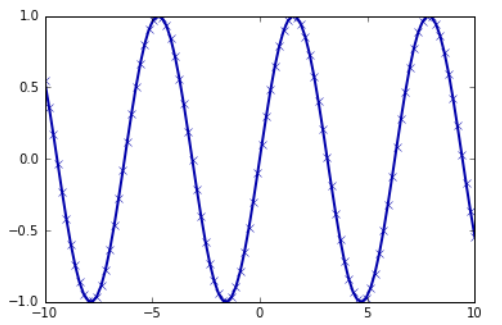
\includegraphics[scale=0.55]{Imagen_Machine/Seno}
	\caption{Gráfico de la función del seno usando matplotlib}
	\label{Seno}
\end{figure} 
                            %   wrangling   =   discusión  

\subsubsection{pandas}

 {\ttfamily pandas\index{pandas}} es basada en una estructura de datos llamada DataFrame, que es modelado como la DataFrame del software $R$. En términos sencillos, una DataFrame  panda  es una tabla, similar para una hoja de cálculo de Excel.  
   {\ttfamily pandas} provee un gran alcance de métodos para modificar e operar sobre esta tabla; en particular, permite  consultas con  SQL-like  y  asociacion  de tablas. En contraste con {\ttfamily NumPy}, que requiera que todas las entradas en el arreglo sean del mismo tipo,  {\ttfamily pandas} permite que cada columna sea un tipo separado (por ejemplo, enteros, fechas, números flotante, y cadenas de caracteres (strings) ). 
   Otra herramienta valiosa provista por pandas es su capacidad para tratar una gran variedad de formatos de archivo y bases de datos, como SQL, archivos de Excel, y archivos separado por comas (CSV).  Entrar  en detalle acerca de la funcionabilidad de {\ttfamily pandas} está fuera del alcance de este libro. Sin embargo, el texto \href{https://www.oreilly.com/library/view/python-for-data/9781449323592/}{\color{vino} Python for Data Analysis}  de  Wes McKinney (O’Reilly, 2012) provee una buena  guía.
   A continuación se presenta  un   ejemplo sencillo de una  DataFrame usando un diccionario:\\

\begin{lstlisting}	

In[7]:  import pandas as pd
        
        # create a simple dataset of people
        data = {'Name': ["John", "Anna", "Peter", "Linda"],
	            'Location' : ["New York", "Paris", "Berlin", "London"],
     	        'Age' : [24, 13, 53, 33]
               }
        
        data_pandas = pd.DataFrame(data)
        # IPython.display allows "pretty printing" of dataframes
        # in the Jupyter notebook
        #    display(data_pandas),   tambien muestra la tabla  display( )
        print(data_pandas) 
          
\end{lstlisting}  
    %     bonita =  pretty    

\noindent Este instrución  produce el siguiente resultado:
\begin{figure}[h!]
%	\centering
	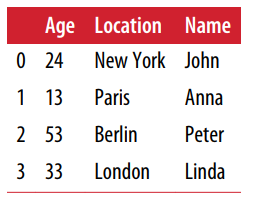
\includegraphics[scale=0.65]{Imagen_Machine/Captura}
%	\caption{Dataframe}
	\label{dataframe1}
\end{figure} 


Hay varias formas posibles de consultar esta tabla. Por ejemplo:\\

\begin{lstlisting}

In[8]:  # Select all rows that have an age column greater than 30
        display(data_pandas[data_pandas.Age > 30])

\end{lstlisting}

\noindent Esto produce el siguiente resultado:
\begin{figure}[h!]
	%\centering
	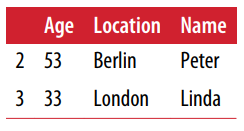
\includegraphics[scale=0.65]{Imagen_Machine/Dataframe2}
	%\caption{Dataframe}
	\label{dataframe2}
\end{figure} 



\subsubsection{mglearn}
 mglearn:\index{mglearn} Funciones  de ayuda para el libro "{}Introducción al aprendizaje automático con Python"{}.   Este libro viene con un código adjunto, que puede encontrar en \href{https://github.com/amueller/introduction_to_ml_with_python}{\color{vino} GitHub}.  El código adjunto incluye no sólo todos los ejemplos que se muestran en este libro, sino también
la librería {\ttfamily mglearn\index{mglearn}}.
  Ésta es una librería de utilidad funcional  que se emplea en este libro, así 
 que no saturamos listas de códigos con detalles para graficar  y carga los datos. Si
 está interesado, puede ver todas las funciones en el repositorio, pero los detalles del módulo  {\ttfamily mglearn}  no es realmente importante para el desarrollado del material de este libro.  Si hace un llamado a {\ttfamily mglearn} con el código, generalmente es una forma de hacer un trabajo rápido  y elegante, o para obtener  algunos datos interesantes.\\
        %     Throughout  =    A través   

  
\begin{minipage}[t]{0.2\textwidth}
	\centering\raisebox{\dimexpr \topskip-\height}{%
		
\includegraphics[width=\textwidth]{Imagen_Machine/Pajaro.png}}
\end{minipage}%\hfill
\begin{minipage}[t]{0.75\textwidth} 
	{\scriptsize		
		A lo largo del libro hacemos un amplio uso de NumPy, pandas  y matplotlib. 
		Todo el código asumirá las siguientes importaciones:
				
		\vspace{0.3cm} {\ttfamily
			
			{ \color{blue} 	importar numpy como np
				
				importar matplotlib.pyplot como plt
				
				importar pandas como pd
				
				importar mglearn\\  }  } 		

\begin{singlespace}
	También asumimos que ejecutará el código en un cuaderno Jupyter en línea con  \%matplotlib  habilitado para mostrar gráficos. Si no utiliza el cuaderno o estos comandos en linea (mágia de \%matplotlib), 	tendrás que usar el comando  plt.show  para  mostrar realmente cualquiera  de las figuras.
\end{singlespace}
}
\end{minipage}
  
   
  
   
   
\subsection{Python 2 Versus Python 3}

Hay dos versiones principales de Python\index{Python 2 Vs Python 3} que se usan ampliamente en este momento: Python 2 (más preciso, 2.7) y Python 3 (con la última versión 3.5 ó 3.7.4   en el momento de escribir y traducir este texto). Esto a veces conduce a cierta confusión.  Python 2 ya no está activamente en desarrollo,  pero debido a que Python 3 contiene cambios importantes, el código de Python 2 generalmente no no corre en Python 3. Si es Usted nuevo en Python o está comenzando un nuevo proyecto desde cero, recomendamos usar la última versión de Python 3 sin cambios.   Si Usted tiene una base de código grande en la que confía que está escrita para Python 2, está excusado de actualizarlo por ahora. Sin embargo, debe intentar migrar a Python 3 tan pronto como sea posible.  Si usted no tiene que interactuar con software heredado,  definitivamente debería usar a la Python 3.  Todo el código en este libro está escrito de una manera que funciona para ambas versiones. Sin embargo, el la salida exacta puede diferir ligeramente bajo  Python 2.

\subsubsection{Versiones utilizadas en este libro}

%  Previamente mencionamos  en las librerías
Las versiones usadas en este texto son las siguientes:
\begin{lstlisting}
In[9]:  import sys
        print("Python version: {}".format(sys.version))

        import pandas as pd
        print("pandas version: {}".format(pd.__version__))

        import matplotlib
        print("matplotlib version: {}".format(matplotlib.__version__))

        import numpy as np
        print("NumPy version: {}".format(np.__version__))

        import scipy as sp
        print("SciPy version: {}".format(sp.__version__))

        import IPython
        print("IPython version: {}".format(IPython.__version__))

        import sklearn
        print("scikit-learn version: {}".format(sklearn.__version__)) 
 
Out[9]:
    Python version: 3.7.4 (default, Aug  9 2019, 18:22:51) [MSC v.1915 32 bit (Intel)]
    pandas version: 0.25.1
    matplotlib version: 3.1.1
    NumPy version: 1.16.5
    SciPy version: 1.3.1
    IPython version: 7.8.0
    scikit-learn version: 0.21.1
\end{lstlisting}                        %         match  = coincidir encuentro
Si bien no es importante hacer coincidir exactamente estas versiones, usted debería tener una versión de scikit-learn que sea tan reciente como la que usamos. Ahora que tenemos todo establecido o configurado,  podemos ejecutar nuestra primera aplicación de  Aprendizaje Automático.\\


\begin{minipage}[t]{0.2\textwidth}
	\centering\raisebox{\dimexpr \topskip-\height}{%
		
\includegraphics[width=\textwidth]{Imagen_Machine/Escorpion}}
\end{minipage}%\hfill
\begin{minipage}[t]{0.75\textwidth} 
	{\scriptsize 
En este libro se supone que usted tiene la versión 0.18,  0.21.1  o  la más reciente de scikitlearn. El módulo model\_selection se agregó en 0.18. Si usas una versión anterior de scikit-learn, necesitará
ajustar lo más importante de este módulo.}
\end{minipage}\\



\section{Primera Aplicación:\\	
	 Clasificación de la especie de flores Iris}

En esta sección, empezaremos con una aplicación muy simple de aprendizaje automático y crearemos el primer modelo. Durante el proceso, introduciremos algunos términos y conceptos básicos.\\

Supongamos un botánico que se interesa en  distinguir  algunas especies de las flores  Iris que encontró. El ha coleccionado algunas medidas asociadas con cada una de las flores iris: La longitud y anchura tanto de los de los pétalos como la de los sépalos, todo medido en los centímetros (ver figura \ref{Iris} ).



\begin{figure}[h!]
	\centering
	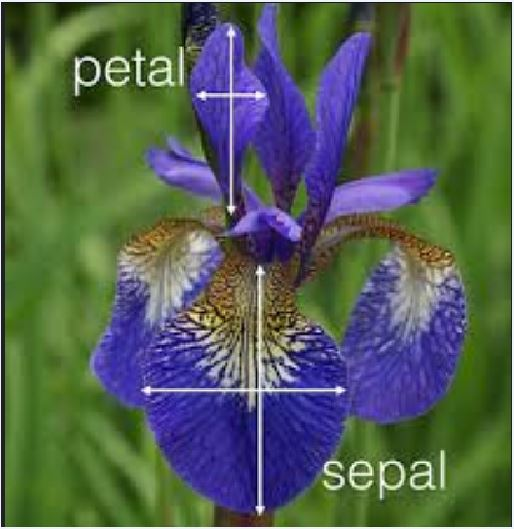
\includegraphics[scale=0.5]{Imagen_Machine/Iris}
	\caption{Partes de una flor especie Iris}
	\label{Iris}
\end{figure} 


Él también tiene las medidas de algunos flores iris que han sido previamente identificados por un botánico experto,  perteneciente a la especie  setosa, versicolor, y virginica (ver figura \ref{Especie}) Con esas medidas, él puede estar seguro a cuál especie pertenece cada iris. Supongamos que éstas son las únicas especie que nuestro botánico aficionado encontrará en su hábitat natural. 

Nuestro objetivo es construir un modelo de aprendizaje automático que pueda aprender de las mediciones
de estas flores iris cuya especie es conocida, para que podamos predecir la especie para una nueva flor
iris.\\


\begin{figure}[h!]
	\centering
	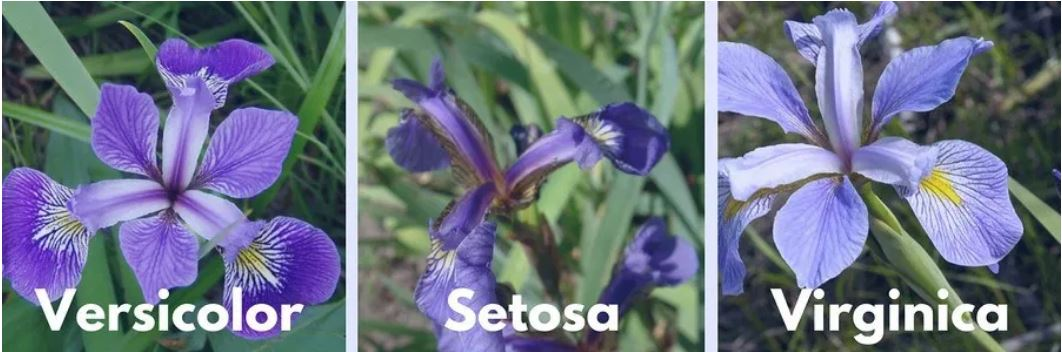
\includegraphics[scale=0.5]{Imagen_Machine/Especie}
	\caption{Tres especies de flores Iris}
	\label{Especie}
\end{figure} 


Ya que tenemos las  medidas para las cuales conocemos la especie correcta de iris, éste es un problema de  de aprendizaje supervisado. En este problema, queremos predecir una  opciones de la especie de iris. Éste es un ejemplo de un problema de clasificación. Las posibles salidas (diferente especies de iris) son llamadas clases. 

Cada iris en el dataset pertenece a una de tres clases (setosa, versicolor, o virginica), este ejemplo es un problema de clasificación de tres clases. La salida deseada para un único punto de datos (una flor iris) es la especie de esta flor. Para un punto particular de la data, la especie a la que  pertenece es llamada  etiqueta, su etiqueta respectivamente.


\subsection{Data Iris}

Los datos que destinaremos para este ejemplo es la Dataset Iris, un conjunto de datos\index{dataset} (dataset) clásico en  las estadísticas y ahora en el aprendizaje automático. Está incluido en scikit-learn en el módulo de datasets. Lo podemos cargar llamando la función load\_iris:\\

\begin{lstlisting}
In[10]:  from sklearn.datasets import load_iris
         iris_dataset = load_iris()
\end{lstlisting}


El objeto  iris  que retorna al cargar  la data iris (load\_iris) es un objeto tipo manojo, lo cual es muy similar a un diccionario. Éste contiene claves y valores:\\

\begin{lstlisting}
In[11]:  print("Keys of iris_dataset: \n{}".format(iris_dataset.keys()))

Out[11]:  
    Keys of iris_dataset:
    dict_keys(['target_names', 'feature_names', 'DESCR', 'data', 'target'])
\end{lstlisting}

    %  feel free to look up the rest yourself

El valor de la  clave DESCR, es una descripción muy breve del conjunto de datos (dataset). Mostramos el inicio de la descripción aquí (usted puede ver el resto):\\

\begin{lstlisting}
In[12]:  print(iris_dataset['DESCR'][:193] + "\n...")

Out[12]:

    Iris Plants Database
    ====================
    Notes
    ----
    Data Set Characteristics:
       :Number of Instances: 150 (50 in each of three classes)
       :Number of Attributes: 4 numeric, predictive att
    ...
    ----
\end{lstlisting} 

El valor de la clave  {\ttfamily {target\_names}} es un arreglo  strings (matriz de cadena), conteniendo las especies de  las flores que queremos predecir:\\

\begin{lstlisting}
In[13]:  print("Nombre del objetivo: {}".format(iris_dataset['target_names']))

Out[13]:

Nombre del objetivo: ['setosa' 'versicolor' 'virginica']
\end{lstlisting}



El valor de {\ttfamily {feature\_names,}}  nombre de la característica es una lista de strings, que da la descripción de cada característica:\\

\begin{lstlisting}
In[14]:  print("Nombres de las Caracteristicas: \n{}".format(
                 iris_dataset['feature_names']))

Out[14]:

   Nombres de las Caracteristica:
   ['sepal length (cm)', 'sepal width (cm)', 'petal length (cm)',
    'petal width (cm)']
\end{lstlisting}

La data  contiene las medidas numéricas del ancho y longitud del sépalo y del pétalo,
  en un arreglo NumPy:\\


\begin{lstlisting}
In[15]:  print("Tipo de data: {}".format(type(iris_dataset['data'])))

Out[15]:

    Tipo de data: <class 'numpy.ndarray'>
\end{lstlisting}


Las filas en el arreglo de la data  corrresponden a las flores, mientras que las columnas representan las cuatro medidas que fueron tomadas a cada flor: 





\begin{lstlisting}
In[16]:  print("Forma de la data:  {}".format(iris_dataset['data'].shape))

Out[16]:
  
    Forma de la data:  (150, 4)
\end{lstlisting}



Vemos que el areglo (array) contiene las medidas de 150 flores diferentes. Recuerde
el item individual es llamado muestra en el aprendizaje automático, y sus propiedades son llamadas características. La forma del conjunto  de datos (array) es el número de muestras multiplicada por el número de características. Ésta es una convención en scikit-learn, y se asumirá que sus datos siempre están en esta forma. Aquí están los valores de característica para las primeras cinco muestras:\\

\begin{lstlisting}
In[17]:  print("Primeras 5 columnas de la data:\n{}".format(
                  iris_dataset['data'][:5]))

Out[17]:

   Primeras 5 columnas de la data:
   [[ 5.1  3.5  1.4  0.2]
    [ 4.9  3.   1.4  0.2]
    [ 4.7  3.2  1.3  0.2]
    [ 4.6  3.1  1.5  0.2]
    [ 5.   3.6  1.4  0.2]]
\end{lstlisting}



A partir de estos datos, podemos ver las primeras cinco flores tienen un ancho de pétalo de 0.2 cm
y que la primera flor tiene el sépalo más largo, de 5,1 cm. La matriz objetivo contiene las especies de cada una de las flores que se midieron, también como una matriz NumPy (NumPy array): \\

\begin{lstlisting}
In[18]:  print("Tipo de objetivo: {}".format(type(iris_dataset['target'])))

Out[18]:

    Tipo de objetivo: <class 'numpy.ndarray'>
\end{lstlisting}

  El objetivo es un arreglo unidimensional, con un entero por cada flor:\\ 

\begin{lstlisting}
In[19]:  print("Forma de objetivo: {}".format(iris_dataset['target'].shape))

Out[19]:

    Forma de objetivo: (150,)
\end{lstlisting}

  Las especies están codificadas con enteros del 0 al 2:\\

\begin{lstlisting}
In[20]:  print("Objetivo:\n{}".format(iris_dataset['target']))

Out[20]:
\end{lstlisting}
{ \ttfamily  	 {\scriptsize{ 
			
			Objetivo:
			
			[0 0 0 0 0 0 0 0 0 0 0 0 0 0 0 0 0 0 0 0 0 0 0 0 0 0 0 0 0 0 0 0 0 0 0 0 0
			
			\hspace{0.2cm}0 0 0 0 0 0 0 0 0 0 0 0 0 1 1 1 1 1 1 1 1 1 1 1 1 1 1 1 1 1 1 1 1 1 1 1 1
			
			\hspace{0.2cm}1 1 1 1 1 1 1 1 1 1 1 1 1 1 1 1 1 1 1 1 1 1 1 1 1 1 2 2 2 2 2 2 2 2 2 2 2
			
			\hspace{0.2cm}2 2 2 2 2 2 2 2 2 2 2 2 2 2 2 2 2 2 2 2 2 2 2 2 2 2 2 2 2 2 2 2 2 2 2 2 2
			
			\hspace{0.2cm}2 2] \\
			
}}}


El significado de los números estan dados por el arreglo   de la data iris 
 {\ttfamily iris['target\_names']}:  0 para Setosa, 1 para versicolor, y 2 para virginica.


%    trust   =  confianza
%    thumb    = general 

  %        performance  =  rendimiento 
  
\subsection{Mediendo el éxito: Datos para entrenamiento y prueba}

Queremos  construir un modelo con aprendizaje automático usando esta información que pueda predecir a la especie de iris para un nuevo conjunto de medidas. Pero antes de aplicar nuestro modelo a medidas nuevas, necesitamos conocer si realmente este modelo funciona bien, y si podemos confiar en sus predicciones. \\

% capital X,   lowercase y

Desafortunadamente, no podemos usar los datos que se emplean para construir el modelo para evaluarlo. Esto se debe a que el modelo siempre puede recordar simplemente todo el conjunto de entrenamiento, y por lo tanto siempre predecirá la etiqueta correcta para cualquier punto del conjunto de entrenamiento. Este
"{}recordatorio"{} no permite  indicar si el modelo se generalizará bien (en  otras palabras, si también funcionará bien con datos nuevos).


Para evaluar el rendimiento del modelo, lo tratamos o ejecutamos con nuevos datos (datos que no han visto
antes) para lo cual tenemos etiquetas. Esto generalmente se hace dividiendo los datos etiquetados que
hemos reunido (en este caso,  150 medidas de flores) en dos partes. Una parte de los datos se utilizan para construir el modelo de aprendizaje automático y se denominan datos de capacitación\index{conjunto de entrenamiento} o conjunto de entrenamiento. El resto de los datos se utilizarán para evaluar qué tan bien funciona el modelo; esta se llama datos de prueba, conjunto de prueba\index{conjunto de prueba} o conjunto de retención (test data, test set, or hold-out set).\\

scikit-learn contiene una función que baraja (seudoaleatorio) el conjunto de datos y lo divide: 
la función es {\ttfamily train\_test\_split}.  Esta función extrae el 75\% de las filas de los datos como
conjunto de entrenamiento, junto con las etiquetas correspondientes; y el 25\% restante
de los datos, junto con las etiquetas restantes, se declara como el conjunto de prueba. En este caso se ha decidido la cantidad de datos que desea dejar para el entrenamiento o capacitación  y  prueba del modelo,  con un criterio un poco arbitrario, sin embargo, usar un conjunto de prueba que contenga el 25\% de los datos es una buena regla general.   En scikit-learn, los datos generalmente se denotan con una $X$ mayúscula, mientras que las etiquetas se denotan por una $y$ minúscula. Esto está inspirado en la formulación estándar $f(x) = y$ en matemáticas, donde $x$ es la entrada de una función e $y$ es la salida. Siguiendo las convenciones de las matemáticas, usamos una $X$ mayúscula porque los datos son un arreglo bidimensional (un
matriz) y una $y$  minúscula  porque el objetivo es un arreglo unidimensional (un vector).


Apliquemos la instrucción {\ttfamily train\_test\_split} sobre nuestros datos y asignemos las salidas usando la siguiente  nomenclatura:\\

\begin{lstlisting}
In[21]:  from sklearn.model_selection import train_test_split
         X_train, X_test, y_train, y_test = train_test_split(
              iris_dataset['data'], iris_dataset['target'], random_state=0)

\end{lstlisting}


Antes de realizar la división, la función {\ttfamily train\_test\_split}  baraja el conjunto de datos utilizando un generador de números pseudoaleatorios. Si sólo tomamos los últimos 25\% de los datos como un conjunto de prueba, el conjunto de datos para la prueba  tendrían sólo la etiqueta 2, ya que los puntos de datos están ordenados por la etiqueta (observe la salida para  {\ttfamily iris['target']}  mostrada anteriormente). Usando un conjunto de prueba que sólo contenga una de las tres clases no nos dirá mucho sobre qué tan bien generaliza el modelo, entonces barajamos nuestros datos para asegurarnos de que los datos de prueba contengan datos de todas las clases.\\


Para asegurarnos  que obtendremos la misma salida si ejecutamos la misma función varias veces, proporcionamos al generador de números pseudoaleatorios una semilla fija usando el parámetro {\ttfamily random\_state}. Esto hará que el resultado sea determinístico, por lo que esta línea siempre tiene el mismo resultado. En este trabajo  fijaremos el {\ttfamily random\_state}, siempre que usemos un procedimiento aleatorio.\\



La salida de la función {\ttfamily train\_test\_split} \:es\: {\ttfamily X\_train, X\_test, y\_train}  y
{\ttfamily y\_test}, que son todos los arreglos {\ttfamily NumPy}.  {\ttfamily X\_train} contiene el 75\% de las filas del conjunto de datos,  y {\ttfamily X\_test} contiene el 25\% restante:\\

\begin{lstlisting}
In[22]:  print("X_train shape: {}".format(X_train.shape))
         print("y_train shape: {}".format(y_train.shape))

Out[22]:

    X_train shape: (112, 4)
    y_train shape: (112,)

In[23]:  print("X_test shape: {}".format(X_test.shape))
         print("y_test shape: {}".format(y_test.shape))

Out[23]:
    
    X_test shape: (38, 4)
    y_test shape: (38,)

\end{lstlisting}





      %   without = sin
\subsection{Primer paso: Analizar los datos}


Antes de construir un modelo de aprendizaje automático, es buena idea inspeccionar los datos,
para ver si la tarea se puede resolver fácilmente sin aprendizaje automático, o si la información deseada
podría no está contenida en los datos. Además, inspeccionar sus datos es una buena manera de encontrar anormalidades y peculiaridades.  Tal vez algunas de sus flores iris se midieron usando pulgadas y no centímetros, por ejemplo. En el mundo real, las inconsistencias en los datos y mediciones inesperadas son muy comunes.


Una de las mejores formas de inspeccionar los datos es visualizarlos. Una forma de hacerlo es mediante el uso de un gráfico de dispersión. Un diagrama de dispersión\index{gráfico de dispersión} de los datos coloca una característica a lo largo del eje $X$ y otra a lo largo del eje $Y$, y dibuja un punto para cada  datos (muestra). Lamentablemente, la pantalla de la computadora  tiene  sólo dos dimensiones,   lo que nos permite trazar sólo dos o tal vez tres características a la vez.  Es difícil trazar conjuntos de datos con más de tres características de esta manera. 

 
Una forma de tratar este problema es hacer un diagrama por pares, para analizar todos los pares posibles  de características. Si tiene una pequeña cantidad de características, como las cuatro que tenemos aquí, esta es bastante razonable. Sin embargo, debe tener en cuenta que un gráfico de pares no muestra la interacción de todas las funciones a la vez, por lo que algunos aspectos interesantes de los datos tal  vez no se revelarán al visualizarlo de esta manera.



La Figura \ref{pares} es un diagrama de pares dos a dos de las características en del conjunto de entrenamiento. Los puntos de datos están coloreados según la especie a la que pertenece la flor iris. Para crear  el gráfico, primero convertimos el arreglo {\ttfamily NumPy} en una { \ttfamily  Dataframe pandas. \:   pandas}  tiene una función para crear gráficos de pares llamado  {\ttfamily scatter\_matrix}. La diagonal de esta matriz se llena con los histogramas de cada característica:\\


\begin{lstlisting}
In[24]:  # create dataframe from data in X_train
         # label the columns using the strings in iris_dataset.feature_names
         iris_dataframe = pd.DataFrame(
                              X_train, columns=iris_dataset.feature_names)
         # create a scatter matrix from the dataframe, color by y_train
         grr = pd.scatter_matrix(iris_dataframe, c=y_train, figsize=(15, 15), 
                                 marker='o', hist_kwds={'bins': 20}, s=60, 
                                 alpha=.8, cmap=mglearn.cm3)
                             
\end{lstlisting}


\begin{figure}[h!]
	\centering
	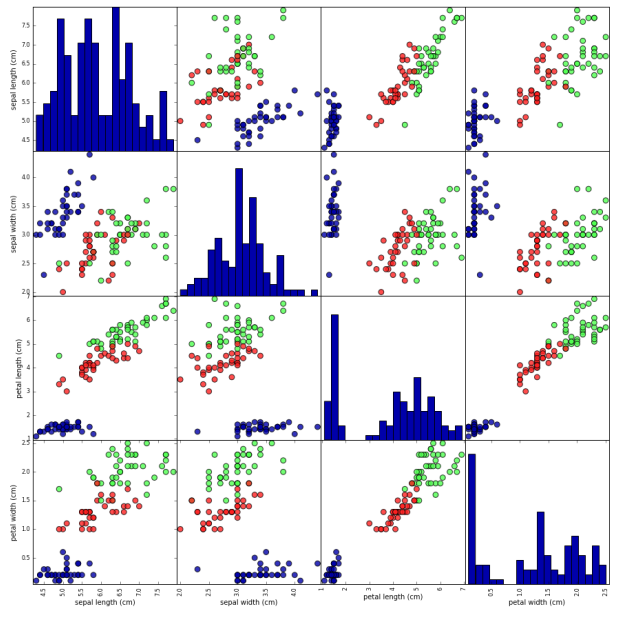
\includegraphics[scale=0.85]{Imagen_Machine/pares}
	\caption{Gráfico por pares de la dataset Iris, coloreado por etiquetas de clase}
	\label{pares}
\end{figure} 


De los gráficos en la figura \ref{pares}, podemos ver que las tres clases parecen estar relativamente bien separadas usando las medidas de sépalos y pétalos. Esto significa que un modelo de aprendizaje automático
probablemente podrá aprender a separarlos.



\subsection{Construyendo el Primer Modelo: método del k-Nearest Neighbors}

  %   k-vecinos más cercanos
Ahora podemos comenzar a construir el modelo real de aprendizaje automático. Hay muchos algoritmos de clasificación en {\ttfamily scikit-learn}  que podríamos usar. Aquí usaremos el clasificador del k-vecinos más cercanos (k-nearest neighbors\index{k-Nearest Neighbors}),  que es fácil de entender.   La construcción de este modelo sólo consiste en almacenar el conjunto de entrenamiento. Para hacer una predicción de un nuevo punto de datos, el algoritmo encuentra el punto en el conjunto de entrenamiento más cercano al nuevo punto, y luego asigna la etiqueta de este punto de entrenamiento al nuevo punto de datos.

La $k$ en el  k-vecinos más cercanos significa que en lugar de usar sólo el vecino más cercano
para el nuevo punto de datos, podemos considerar cualquier número fijo $k$ de vecinos en el conjunto de entrenamiento (por ejemplo, los tres o cinco vecinos más cercanos). Entonces, podemos hacer una predicción
utilizando la clase mayoritaria entre estos vecinos. Entraremos en más detalles sobre
esto en el Capítulo \ref{Cap2}; por ahora, usaremos un sólo vecino.\\


Todos los modelos de aprendizaje automático en {\ttfamily scikit-learn} son implementados en sus propias clases, y es llamado   {\ttfamily Estimator} de clases.  El algoritmo de clasificación del k-vecino más cercano es implementado en la clase  {\ttfamily KNeighboursClassifier}  en el módulo de {\ttfamily neighbors}.  Antes de usar el modelo, necesitamos instanciar la clase en un objeto\index{instanciar la clase}. Esto es cuando configuramos cualquier parámetro del modelo. 

El parámetro más importante  del  {\ttfamily KNeighboursClassifier}  es el número de vecinos, que estableceremos en 1:\\

\begin{lstlisting}
In[25]:  from sklearn.neighbors import KNeighborsClassifier
         knn = KNeighborsClassifier(n_neighbors=1)

\end{lstlisting}


  %    hold   =  sostiene  aguanta  guarda

El objeto knn encapsula el algoritmo que se usará para construir el modelo a partir de
la data de entrenamiento, así como el algoritmo para hacer predicciones sobre nuevos puntos de datos. Este
también contienen la información que el algoritmo ha extraído de los datos de entrenamiento.
 
En el caso de {\ttfamily KNeighboursClassifier}, sólo almacenará el conjunto de entrenamiento.
Para construir el modelo en el conjunto de entrenamiento, llamamos al método de ajuste del objeto knn,
que toma como argumentos el arreglo {\ttfamily NumPy \: X\_train} que contiene los datos de entrenamiento y
el arreglo NumPy y\_train de las etiquetas de entrenamiento correspondientes: \\

\begin{lstlisting}
In[26]:  knn.fit(X_train, y_train)

Out[26]:

    KNeighborsClassifier(algorithm='auto', leaf_size=30, metric='minkowski',
               metric_params=None, n_jobs=1, n_neighbors=1, p=2,
               weights='uniform')
\end{lstlisting}
    %        worry   =   preocupación 


El método de ajuste devuelve el objeto knn en sí (y lo modifica en su lugar), por lo que obtenemos una representación string\index{cadena de caracteres} (cadena de caracteres) de nuestro clasificador. La representación nos muestra qué parámetros fueron utilizados en la creación del modelo. Casi todos son valores predeterminados, pero puede también encontrar {\ttfamily n\_neighbours = 1}, que es el parámetro que seleccionamos. La mayoría de los modelos en scikit-learn tiene muchos parámetros, pero la mayor parte de ellos ya son  optimizaciones de velocidad o para casos de uso muy especiales. No tienes que preocuparte por los demás parámetros mostrados en esta representación.   Imprimir un modelo scikit-learn puede producir string  muy largas, pero no te dejes intimidar por estas. Cubriremos todo lo importante referente a parámetros en el Capítulo \ref{Cap2}. En el resto de este libro, no mostraremos el resultado  de ajuste porque no contiene ninguna información nueva.\\
         %  wild  = descabellado

\subsection{Haciendo Predicciones}

Ahora podemos hacer predicciones usando este modelo en nuevos datos para los cuales podríamos no conocer las etiquetas correctas. Imagina que encontramos un iris en la naturaleza con una longitud de sépalo de 5 cm, con  ancho de sépalo igual a 2,9 cm, una longitud de pétalo de 1 cm y un ancho de pétalo de 0,2 cm. ¿Qué especie de iris sería esta? Podemos poner estos datos en un arreglo  NumPy,  nuevamente  calcular la forma, es decir, el número de muestras (1) multiplicado por el número de características (4):\\

\begin{lstlisting}
In[27]:  X_new = np.array([[5, 2.9, 1, 0.2]])
         print("X_new.shape: {}".format(X_new.shape))

Out[27]:

    X_new.shape: (1, 4)
\end{lstlisting}



Observe  que realizamos las mediciones de esta flor individual en una fila en un arreglo NumPy bidimensional, ya que {\ttfamily scikit-learn}  siempre espera arrreglos bidimensionales para los datos.
Para hacer una predicción, llamamos el método de predicción del objeto knn:\\

\begin{lstlisting}
In[28]:  prediction = knn.predict(X_new)
         print("Predicion: {}".format(prediction))
         print("Nombre del objetivo estimado: {}".format(
                iris_dataset['target_names'][prediction]))

Out[28]:

    Predicion: [0]
    Nombre del objetivo estimado: ['setosa']
\end{lstlisting}


El modelo predijo que esta nueva flor iris pertenece a la clase 0, lo que significa que su especie es setosa.  Pero, ¿cómo sabemos si podemos confiar en nuestro modelo?  No sabemos la especie correcta de esta muestra, ¡cuál es el objetivo para completar de construir el modelo!


\subsection{Evaluación del modelo}

Aquí es donde entra el conjunto de prueba que creamos anteriormente. Estos datos no se utilizaron para construimos el modelo, pero conocemos la especie correcta para cada iris en el conjunto de prueba (test set).

Por lo tanto, podemos hacer una predicción para cada iris en el conjunto de prueba y compararlo contra su etiqueta (la especie conocida).  Podemos medir qué tan bien funciona el modelo calculando la  exactitud (accuracy)\index{exactitud}, que es la fracción de flores para la que se predijo la especie correcta:\\

\begin{lstlisting}
In[29]:  y_pred = knn.predict(X_test)
         print("Test set predictions:\n {}".format(y_pred))

Out[29]:

Test set predictions:
[2 1 0 2 0 2 0 1 1 1 2 1 1 1 1 0 1 1 0 0 2 1 0 0 2 0 0 1 1 0 2 1 0 2 2 1 0 2]

In[30]:  print("Test set score: {:.2f}".format(np.mean(y_pred == y_test)))

Out[30]:

    Test set score: 0.97
\end{lstlisting}


También podemos  usar el método de puntuación\index{método de puntuación} (score\index{score})  del objeto {\ttfamily knn}, que calculará la exactitud en el conjunto de prueba:\\


\begin{lstlisting}
In[31]:  print("Puntuacion del conjunto de pruebas: {:.2f}".format(
                 knn.score(X_test, y_test)))

Out[31]:

    Puntuacion del conjunto de pruebas: 0.97
\end{lstlisting}


Para este modelo, la exactitud del conjunto de prueba (test set) es de aproximadamente 0.97, lo que significa que hicimos la  predicción correcta  para el 97\% de los datos en el conjunto de prueba. Bajo  suposición estadística, esto significa que podemos esperar que nuestro modelo sea correcto el 97\% de la veces para nuevas flores iris.  
 La aplicación para el botánico aficionado, este alto nivel de exactitud significa que nuestro  modelo puede ser lo suficientemente confiable como para usarlo. En capítulos posteriores discutiremos cómo puede mejorar el rendimiento y las advertencias que existen al ajustar un modelo.


  %    trustworthy  =   confiable
  %     caveats     =   advertencias 



\section{Resumen y perspectivas}

Resumiendo lo que aprendido en este capítulo. Comenzamos con una breve introducción
al aprendizaje automático y sus aplicaciones, luego discutimos las diferencias entre
aprendizaje supervisado y no supervisado, y se dió una visión general de las herramientas que veremos
en este libro. Luego, formulamos la tarea de predecir  mediante el uso de medidas físicas  a qué especie  pertenece una nueva flor iris.  Utilizamos un conjunto de datos de mediciones que fue anotado por un experto con la especie correcta para construimos el modelo, convirtiéndolo en una tarea de aprendizaje supervisado. Había tres posibles especies, setosa, versicolor o virginica, que hace de la tarea un problema de clasificación de tres clases. Las especies posibles se denominan clases en el problema de clasificación, y la especie de una flor iris se llama su etiqueta. \\


El conjunto de datos Iris consta de dos arreglos {\ttfamily NumPy}: uno  contiene los datos  $X$  que son
referido  en {\ttfamily scikit-learn}, y el otro contiene los resultados correctos o deseados, llamados $y$.
El arreglo $X$ es una matriz bidimensional de características, con una fila para cada punto de datos o muestra y una columna por caraterística (o variable). El arreglo $y$ es una matriz unidimensional, que  contiene una clase de etiqueta, un número entero que varía de 0 a 2, para cada una de las muestras.


Dividimos el dataset (conjunto de datos\index{dataset}) en dos conjuntos, un conjunto para entrenar y construir el modelo, y el segundo conjunto de prueba para evaluar el modelo, y verificar qué tan bien  generaliza con los nuevos dato (datos no usados).


Elegimos el algoritmo de clasificación del k-vecinos más cercanos,  que hace las predicciones 
para un nuevo punto de datos considerando sus vecinos más cercanos en el conjunto de entrenamiento.  Esto es  implementado en el clasificador {\ttfamily  KNeighboursClassifier}, que contiene tanto el algoritmo que 
construye el modelo como   el algoritmo que realiza hace la predicción.


Instanciamos la clase, configurando los parámetros. Luego construimos el modelo llamando el
método de ajuste, tratando los datos de entrenamiento ({\ttfamily X\_train}) y las salidas de entrenamiento ( {\ttfamily y\_train}) como parámetros. Evaluamos el modelo utilizando el método de puntuación (score method), que calcula la exactitud  del modelo.  Aplicamos el método de puntuación (score method) a los datos de pruebas y conjunto de etiquetas, y encontramos que el modelo es aproximadamente 97\% exacto, lo que significa que es correcto 97\%  de la veces en el conjunto de prueba (test set).\\

En conclusión, el procedimiento generó un modelo que nos brinda  confianza para aplicarlo a nuevos datos (en este caso a nuevas medidas de flores)  y obtener aproximadamente el 97\%  de resultados correctos.\\


A continuación se presenta el resumen del código necesario para entrenar y evaluar el procedimiento:\\


\begin{lstlisting}
In[32]:  X_train, X_test, y_train, y_test = train_test_split(
             iris_dataset['data'], iris_dataset['target'], random_state=0)
         
         knn = KNeighborsClassifier(n_neighbors=1)
         knn.fit(X_train, y_train)
         
         print("Test set score: {:.2f}".format(knn.score(X_test, y_test)))

Out[32]:

    Test set score: 0.97
\end{lstlisting}

   %        snippet  =    fragmento

 Este fragmento contiene el  código nucléo (código básico) para aplicar cualquier algoritmo de aprendizaje automático usando scikit-learn.  Los métodos de ajuste, predicción y puntuación son interfaces comunes de los modelos supervisados es {\ttfamily scikit-learn}, y con los conceptos introducidos en este capítulo,
 pueden aplicar estos modelos a muchas tareas de aprendizaje automático.  En el próximo el capítulo, profundizaremos sobre los diferentes tipos de modelos supervisados en  {\ttfamily scikit-learn} y cómo aplicarlos con éxito.

%\end{document}

\newpage



     % Cargamos los capítulos desde la carpeta Contenido.
   



	
	\chapter{Aprendizaje Supervisado}{\label{Cap2}}

	      %  Capitulo 2 	
	

	%%  Applied Spatial Data Analysis with R  de Roger S. Bivand (Edzer Pebesma y Virgilio Gómez-Rubio) como  
	%%    Analysing  spatial  point patterns in R de  Adrian Baddeley.\\
	

	%% Sistema de información geografica los ordenadores, como software R y GVSIG,
	

\section{Preliminares}            


El  aprendizaje estadístico  supervisado es uno de los más comunes y exitosos tipos de aprendizaje estadístico  (o machine learning). En este capítulo se describe el aprendizaje supervisado con más detalle y se explican algunos algoritmos comunes mismo. En el Capítulo \ref{Cap1}  vimos una introducción al machine learning, con  la clasificación de las Flores Iris en varias especies, de acuerdo con las medidas físicas de las flores.\\

Recordemos que el aprendizaje supervisado es usado cada vez que queremos predecir cierta salida de una entrada dada, siempre te tengamos ejemplos suficientes de pares de entrada y salida  (input{\scriptsize/}output). Se construye el modelo de aprendizaje automático con estos pares de entrada{\scriptsize/}salida, que se encuentran en  la data de entrenamiento o capacitación. El objetivo es hacer predicciones exactas para datos nuevos, nunca antes vistos o tratados.   El aprendizaje supervisado frecuentemente requiere de un esfuerzo humano para construir un conjunto de entrenamiento,  pero ahora  es automatizado y generalmente facilita y acelera el trabajo, que de otra manera sería muy laboriosa y  en algunos casos inviable.


\subsection{Clasificación y Regresión}


Generalmente en el aprendizaje supervisado se consideran dos tipos de problemas más importantes llamados clasificación y regresión.\\

En el problema de clasificación, el objetivo es predecir una clase etiquetada  seleccionada  de una lista predefinidas de posibilidades. En el  Capítulo \ref{Cap1} se presentó la clasificación de las flores iris dentro de tres tipos de  especie  posible. El problema de clasificación algunas veces es separada en dos tipos, clasificación binaria y clasificación multiclase. La clasificación binaria consta exactamente de dos clases, mientras que la multiclase tiene más de dos clases.  Se puede pensar en una clasificación binaria como una prueba para responder una pregunta con dos respuestas, si o no. Un ejemplo práctico de la clasificación binaria es clasificar un correo como spam o no spam. En esta clasificación la tarea en responder, si o no a la pregunta.\\
	


\begin{minipage}[t]{0.2\textwidth}
	\centering\raisebox{\dimexpr \topskip-\height}{%
		
\includegraphics[width=\textwidth]{Imagen_Machine/Pajaro.png}}
\end{minipage}%\hfill
\begin{minipage}[t]{0.75\textwidth} 
	{\scriptsize	
		En la clasificación binaria frecuentemente se habla de una  clase positiva y una clase		
		negativa.	Aquí, la clase positiva no representa beneficio o valor, sólo es objeto		
		de estudio. Así, que cuando vemos  "positivo"  ( spam),  significa clase spam. Designar		
		una de las dos clases como  positiva  es a menudo una materia subjetiva, y específico		
		para el dominio.}
\end{minipage}




El problema de las flores iris, es un ejemplo de  clasificación multiclase.  Otro típico ejemplo de multiclase, es predecir el lenguaje o idioma en qué  está escrito un sitio Web; las clases en este caso son una lista predefinida de posibles idiomas.  \\

En el caso del problema de regresión, el objetivo es predecir un número de tipo punto-flotante  (floating-point number)  en términos de programación y en términos matemático, un número real. Como ejemplo podemos citar, el ingreso anual de una persona por su educación, por su edad, o por el lugar  donde vive. Cuando se predice el ingreso, el valor es una cantidad, y puede ser cualquier número en un rango dado. Otro ejemplo de regresión es predecir el rendimiento de la cosecha de maíz en una granja, dado los atributos previos como rendimiento previo, tiempo (clima) y número de  trabajadores en la granja. El rendimiento nuevamente es un número tipo punto flotante.\\


Una forma fácil de distinguir entre clasificación y regresión es  preguntar si hay algún  tipo de continuidad en la salida. Si hay continuidad en los posibles resultados de salidas, entonces el problema es regresión.  Pensando en el ejemplo de la predicción del ingreso anual. Aquí, claramente hay continuidad en la salida. Si una persona gana 40.000 o 40.001 en un año no hace una diferencia tangible, aun, cuando esas son cantidades diferentes en dinero; si nuestro algoritmo predice 39.999 o 40.001 cuando debe predecir 40.000, no es tan importante.  \\


Por el contrario, para la tarea de reconocimiento del idioma en el sitio web (problema de clasificación), no hay continuidad, entre idiomas, no hay un idioma entre dos. Un sitio web tiene un sólo idioma{\footnote{Pedimos a los lingüistas que disculpen la presentación simplificada de las lenguas como entidades distintas y fijas.}.   

\subsection{Generalización, Sobreajuste,  y Subajuste}  

En el aprendizaje supervisado se  construye un modelo sobre los datos de entrenamiento  que sea capaz de hacer predicciones exactas sobre datos nuevos, que no se han usado en la construcción del modelo pero que   tienen la misma característica de los datos de entrenamiento.

 Si un modelo es capaz de hacer predicciones exactas sobre 	datos nuevos, decimos que es capaz de generalizar\index{capacidad de generalizar} del conjunto de entrenamiento al conjunto de prueba. Así que lo deseado es construir un modelo capaz de generalizar con la mayor exactitud posible.


Por lo general, creamos un modelo de tal manera que pueda hacer predicciones exactas sobre el conjunto de entrenamiento. Si los conjuntos de entrenamiento  y  prueba  tienen  sus  características  comunes  y  semejantes,  se espera que el modelo  también  sea  exacto  en el conjunto de prueba.  Sin embargo, hay algunos casos donde esto puede salir mal. Por ejemplo, si construimos modelos muy complejos y exactos en el conjunto de entrenamiento, el modelo tal vez puede no generalizar bien. \\


Para ilustrar esta situación usaremos el siguiente ejemplo ideado: Supongamos que un aficionado científico de datos quiere predecir si un cliente comprará o no un bote, basándose en los registros de los compradores  de  botes  y  los clientes que sabemos que no están interesados comprar un bote. El objetivo es enviar correos electrónicos promocionales a las personas que probablemente hagan una compra, pero no molestar a aquellos clientes que no estarán interesados.\\


Supongamos que los registros de clientes son los que se muestran en la Tabla \ref{Clientes}.\\



 %                 Example data about customers
 
\begin{table}[h!]
	\centering
	\caption{Ejemplo de datos sobre clientes}
	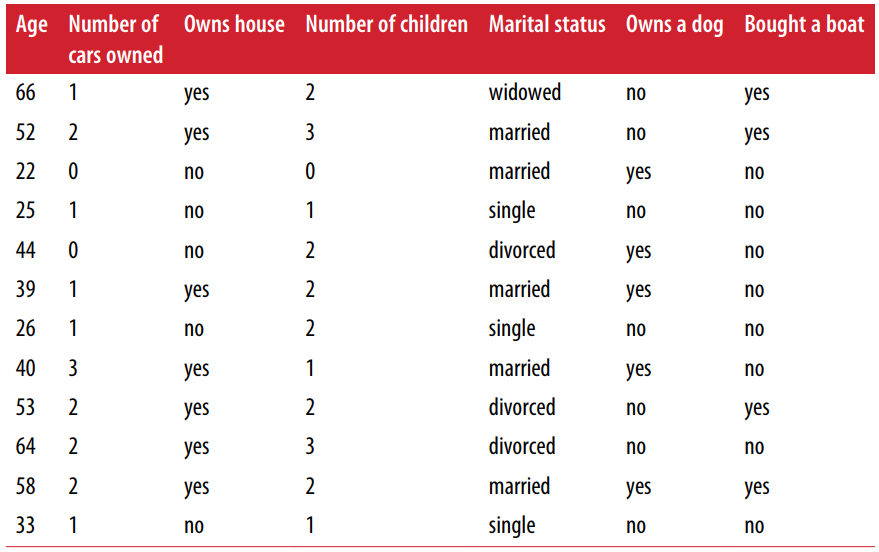
\includegraphics[scale=0.65]{../Imagen_Machine/Clientes}
	\label{Clientes}
\end{table} 


Después de analizar los datos, el científico aficionado se le ocurre la siguiente regla:
"Si el cliente es mayor de 45 años y tiene menos de 3 hijos o no es divorciado, entonces 
quiere comprar un bote". Cuando se le preguntó qué tan bien funciona su regla,
el científico de datos responde:  "¡Es 100 por ciento exacta!" {}   Y de hecho, en los datos de 
la  tabla, la regla es perfectamente exacta. Hay muchas reglas posibles que podríamos
generar  que explicaría perfectamente si alguien en este conjunto de datos quiere comprar o no un bote.  La edad no aparece dos veces en los datos, por lo que podríamos decir que para personas con 66, 52, 53 o 58 años de edad quiere comprar un bote, mientras  que los demás no. Si bien podemos inventar muchas reglas que funcionan bien en estos datos, es importante  resaltar que  no estamos interesados en hacer predicciones para este conjunto de datos; pues, ya sabemos las respuestas para estos clientes.   Queremos saber si los  nuevos clientes  probablemente compran  un bote. Por lo tanto, queremos encontrar una regla que funcione bien para nuevos clientes y que logre una exactitud alta en el conjunto de entrenamiento. Sin embargo, una exactitud del 100 por ciento en el conjunto de entrenamiento generalmente  no nos ayuda en esta situación.  No podemos esperar que la regla propuesta por el aficionado científico de datos, funcionara muy bien con datos nuevos.  Parece demasiado complejo y está  basado  en  muy pocos datos.   Por ejemplo, la parte de la regla  "{}o no está divorciado"{}   se observa en un solo cliente.\\


La única medida para conocer  si un algoritmo funcionará  bien  en nuevos datos es la evaluación en el conjunto de prueba.  Sin embargo, intuitivamente esperamos que los modelos simples  generalicen mejor en los  datos nuevos.  Si la regla era que "las personas mayores de 50 años quieren comprar un bote", y esto explicaría el comportamiento de todos los clientes, confiaríamos más en la regla que involucra niños, estado civil, y además la edad. Por lo tanto, siempre queremos
encontrar el modelo más simple.  Construir un modelo que sea demasiado complejo para la cantidad de información que tenemos, como hizo aficionado el científico, se llama sobreajuste\index{sobreajuste}.  El sobreajuste ocurre cuando se ajusta un modelo demasiado  cerca de las particularidades del conjunto de entrenamiento y se obtiene un modelo que funciona muy bien en el conjunto de entrenamiento pero no es capaz de generalizar para nuevos datos. 
Por otro lado,  si su modelo es demasiado simple, digamos: "Todo cliente que poseen un casa propia,  comprará un bote”,  entonces es posible que no sea capaz de capturar todos los aspectos y variaciones  en los datos, y el modelo funcionará mal incluso en el conjunto de entrenamiento. Elegir un modelo demasiado simple se llama subajuste\index{subajuste}.\\


Cuanto más complejo  sea un modelo  mejor será la capacidad de  predecir sobre  los datos de entrenamiento; sin embargo, si el modelo se hace demasiado complejo, comenzamos a enfocarnos más  en cada punto individual de los datos del conjunto de entrenamiento, y el modelo no funcionará bien sobre los nuevos datos (datos de prueba).\\

Hay un modelo dentro de esta  situación (punto justo  o  Sweet spot)  que producirá el mejor rendimiento de generalización; y este es el modelo que queremos encontrar.\\



En la Figura \ref{complejidad} se ilustra la  compensación entre sobreajuste y subajuste  modelo

\begin{figure}[h!]
	\centering
	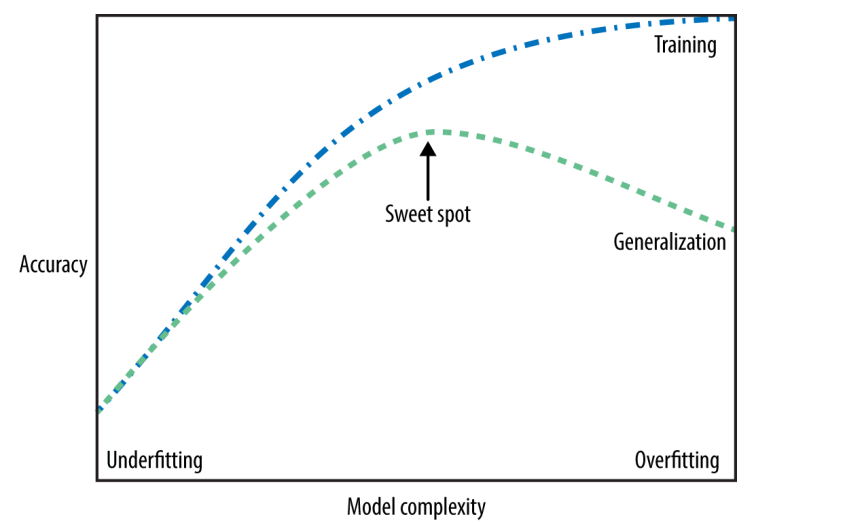
\includegraphics[scale=0.50]{../Imagen_Machine/complejidad}
	\caption{Compensación de la complejidad del modelo contra  la exactitud  de los conjuntos de  entrenamiento  y  la prueba}
	\label{complejidad}
\end{figure} 



\subsubsection{Relación de la complejidad del modelo con el tamaño del conjunto de datos}

Es importante tener en cuenta que la complejidad del modelo está íntimamente ligada a la variación del número
entradas contenidas en el cojunto de entrenamiento: cuando la mayor sea cantidad de puntos en el conjunto de  datos, un modelo más complejo puede generarse sin sobreajuste. Por lo general, coleccionando más puntos en la  data producirá más información, por lo que los conjuntos con más datos permiten construir modelos más complejos. Sin embargo, simplemente duplicar los mismos puntos de datos o recopilar  datos muy similares no ayudará.\\
 

Volviendo al ejemplo de venta de botes, si vemos 10,000 filas más de datos de clientes,
y todos cumplen con la regla: "Si el cliente es mayor de 45 años y tiene menos
de 3 hijos o no está divorciado, entonces quieren comprar un bote", estaríamos mucho más seguros que esta es una buena regla, que cuando se desarrolló utilizando solo las 12 filas de la tabla \ref{Clientes}.\\

  %   wonders =  marabillas

Tener más datos y construir modelos apropiadamente más complejos a menudo puede funcionar de
maravilla para tareas de aprendizaje supervisado. En este libro, nos centraremos en trabajar con
conjuntos de datos de tamaños fijos. Pero en el mundo real, generalmente hay posibilidad de decidir cuantos datos a usar, lo que podría ser más beneficioso para ajustar y afinar el modelo. Por último, le sugerimos que  "Nunca subestimes el poder de más datos".
                   %  tweaking   = ajustar


\section{Ejemplos de algunos conjuntos de datos}


Para ilustrar la aplicación de los diferentes algoritmos, se utilizarán  algunos conjuntos de datos. Conjuntos de datos pequeños y sintéticos (es decir, indeados), diseñado para resaltar
aspectos muy particulares de los algoritmos; y otros conjuntos de datos grandes, como ejemplos del mundo real.\\

Un ejemplo de un conjunto  de clasificación  con dos clases, es la data  sintética    de falsificación de datos (forge dataset), que tiene dos características.


El siguiente código crea un diagrama de dispersión (Figura \ref{DispersionForge}) que visualiza todos de los puntos de datos de este conjunto. El gráfico tiene la primera característica en el eje x y la segunda característica sobre el eje y. Como siempre  en los diagramas de dispersión, cada punto de datos es representado como un punto. El color y la forma del punto indican su clase:\\

\begin{lstlisting}
In[2]:  # generate dataset
        X, y = mglearn.datasets.make_forge()
        # plot dataset
        mglearn.discrete_scatter(X[:, 0], X[:, 1], y)
        plt.legend(["Class 0", "Class 1"], loc=4)
        plt.xlabel("First feature")
        plt.ylabel("Second feature")
        print("X.shape: {}".format(X.shape))

Out[2]:

    X.shape: (26, 2)
\end{lstlisting}



\begin{figure}[h!]
	\centering
	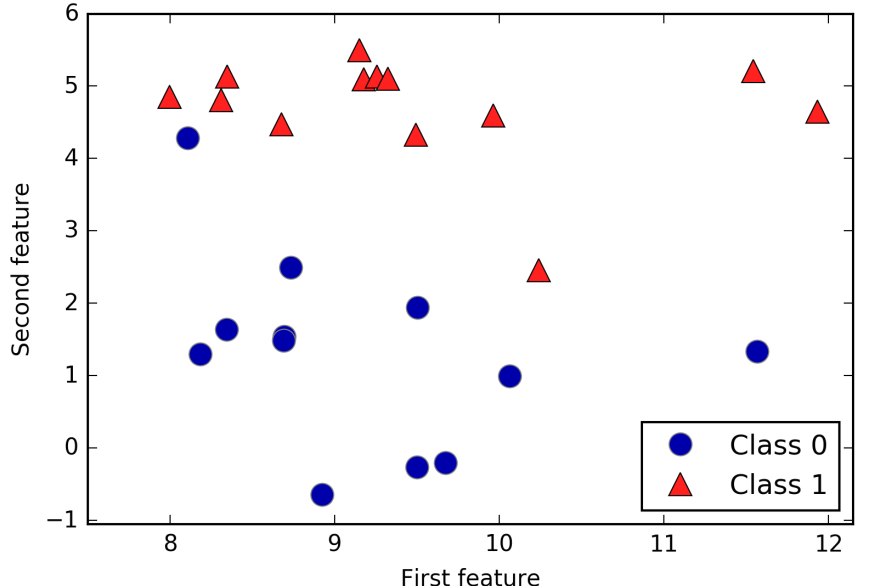
\includegraphics[scale=0.50]{../Imagen_Machine/DispersionForge}
	\caption{Diagrama de dispersión de la dataset  de falsificación de datos (forge dataset)}
	\label{DispersionForge}
\end{figure} 


Como puede ver en  {\ttfamily X.shape}, este conjunto de datos consta de 26 datos, con 2 características.
Para ilustrar el algoritmo de regresión, utilizaremos el conjunto sintético de datos de Onda.
El conjunto de datos de Onda (wave) tiene una única característica de entrada y una variable objetivo  continua (o respuesta)  que queremos modelar. El diagrama en la figura \ref{DispersionForge}  muestra la característica única en el eje x,  y el objetivo de regresión (la salida) en el eje y:\\

\begin{lstlisting}
In[3]:  X, y = mglearn.datasets.make_wave(n_samples=40)
        plt.plot(X, y, 'o')
        plt.ylim(-3, 3)
        plt.xlabel("Feature")
        plt.ylabel("Target")
\end{lstlisting}


\begin{figure}[h!]
	\centering
	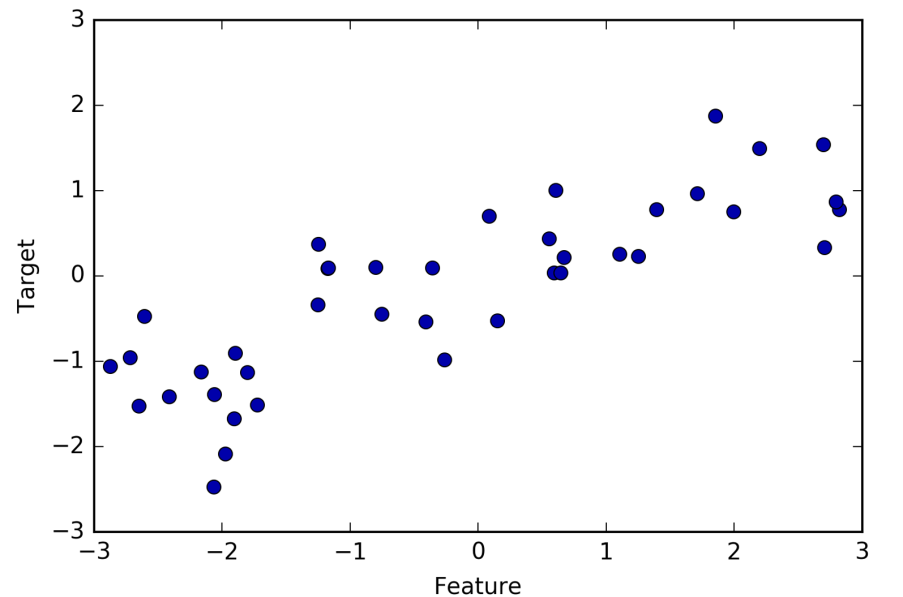
\includegraphics[scale=0.50]{../Imagen_Machine/regresion}
	\caption{Gráfico del conjunto de datos de onda, en el eje $X$ se muestra la
		característica y en  el eje $Y$ el objetivo (respuesta de la regresión).}
	\label{regresion}
\end{figure} 



Utilizamos conjuntos de datos muy simples y de baja dimensión porque se pueden visualizar fácilmente en  dos dimensiones, sin embargo, para base de datos con más de dos características es difícil visualizar. Cualquier intuición derivada de conjuntos de datos con pocas características (también llamada los conjuntos de datos de baja dimensión\index{conjuntos de baja dimensión}) podrían no ayudar en conjuntos de datos con muchas características (conjuntos de datos de alta dimensión\index{conjuntos de alta dimensión}). No obstante, tenga en cuenta, que la inspección de algoritmos en los conjuntos de datos de baja dimensión pueden ser muy instructiva.\\


\begin{minipage}[t]{0.2\textwidth}
	\centering\raisebox{\dimexpr \topskip-\height}{%
		
\includegraphics[width=\textwidth]{Imagen_Machine/Pajaro.png}}
\end{minipage}%\hfill
\begin{minipage}[t]{0.75\textwidth} 
	{\scriptsize	
		Los conjuntos de datos que se incluyen en {\ttfamily scikit-learn} generalmente se almacenan como		
		manojos de objetos, que contienen información sobre el conjunto de datos así como los 		
		datos reales. Todo lo que necesitas saber sobre los objetos tipo manojo de objetos, es que		
		se comportan como diccionarios, con el beneficio adicional de que usted puede acceder a los 		
		valores usando un punto  (como en {\ttfamily bunch.key} en lugar de {\ttfamily bunch['key']}).}
\end{minipage}  \\
%\vspace{0.5cm}

Complementamos estos conjuntos sintéticos y de baja dimensión, con dos conjuntos de datos del mundo real que
están incluidos en {\ttfamily scikit-learn}. Uno de estos es el conjunto de datos del Cáncer de Mama de Wisconsin (Wisconsin Breast Cancer), que registra mediciones clínicas de tumores de cáncer de mama.  Cada tumor está etiquetado como {}"benigno"{}  (para tumores inofensivos) o  {}"maligno"{} (para tumores cancerosos), en este caso la tarea es aprender a predecir si un tumor es maligno basado en las medidas del tejido.\\

Los datos  puede cargarse utilizando la función {\ttfamily{load\_breast\_cancer}} de
 {\ttfamily scikit-learn}:\\

\begin{lstlisting}
In[4]:  from sklearn.datasets import load_breast_cancer
        cancer = load_breast_cancer()
        print("cancer.keys(): \n{}".format(cancer.keys()))

Out[4]:
 
    cancer.keys():
    dict_keys(['feature_names', 'data', 'DESCR', 'target', 'target_names'])

\end{lstlisting}


\noindent La data consiste en 569 puntos o datos, con 30 características cada una:\\


\begin{lstlisting}

In[5]:  print("Forma de la data del cancer: {}".format(cancer.data.shape))

Out[5]:

   Forma de la data del cancer: (569, 30)

 \end{lstlisting} 
 
\noindent  De esos  569 datos, 212  son etiquetados como malignos y 357 como benignos:\\

\begin{lstlisting}

In[6]:  print("Conteos de muestra por clase:\n{}".format(
        {n: v for n, v in zip(cancer.target_names, np.bincount(
               cancer.target))}))
               
Out[6]:

    Conteos de muestra por clase:
    {'benign': 357, 'malignant': 212}
\end{lstlisting}



Para obtener una descripcion semantica del significado de cada característica, podemos verlo con 
el atributo  {\ttfamily feature\_names}:\\

\begin{lstlisting}
In[7]:  print("Nombres de las carateristica:\n{}".format(
                cancer.feature_names))
Out[7]:

    Nombres de las carateristica:
    ['mean radius' 'mean texture' 'mean perimeter' 'mean area'
     'mean smoothness' 'mean compactness' 'mean concavity'
     'mean concave points' 'mean symmetry' 'mean fractal dimension'
     'radius error' 'texture error' 'perimeter error' 'area error'
     'smoothness error' 'compactness error' 'concavity error'
     'concave points error' 'symmetry error' 'fractal dimension error'
     'worst radius' 'worst texture' 'worst perimeter' 'worst area'
     'worst smoothness' 'worst compactness' 'worst concavity'
     'worst concave points' 'worst symmetry' 'worst fractal dimension']
\end{lstlisting}


Si estas interesado en obtener más información al respecto puede ver en 
{\ttfamily{cancer.DESCR}} .\\

También usaremos el conjunto de datos mundo real, el conjunto de datos de Vivienda de Boston (Boston Housing), para la regresión.  La tarea asociada con este conjunto de datos es predecir el valor promedio de las viviendas en algunos barrios de Boston en la década de 1970, utilizando información como la tasa de criminalidad, proximidad al río Charles, accesibilidad a la autopista, etc.  El conjunto de datos contiene 506 puntos de datos, descritos por 13 características:\\

\begin{lstlisting}
In[8]:  from sklearn.datasets import load_boston
        boston = load_boston()
        print("Data shape: {}".format(boston.data.shape))

Out[8]:

    Data shape: (506, 13)
\end{lstlisting}


Nuevamente, puede obtener más información sobre el conjunto de datos en  el atributo {\ttfamily{DESCR}}
de boston. Para nuestros propósitos aquí, expandiremos este conjunto de datos no solo
considera estas 13 medidas como características de entrada, sino  también plantea  todos los productos
entre características (también llamadas interacciones). En otras palabras, no solo consideraremos
tasa de criminalidad y accesibilidad a la autopista como características, sino también el producto de la tasa de criminalidad por la accesibilidad a la autopista.  La inclusión de caractarísticas derivadas o extendidas como estas se denomina ingeniería de características, se discutá en el Capítulo \ref{Cap4} con más detalle. 

El conjunto de datos extendido esta disponible en {\ttfamily mglearn.datasets} y puede ser cargado mediante  la función {\ttfamily load\_extended\_boston}:\\

\begin{lstlisting}
In[9]:  X, y = mglearn.datasets.load_extended_boston()
        print("X.shape: {}".format(X.shape))

Out[9]:

    X.shape: (506, 104)

\end{lstlisting}

 Las 104 características resultantes son las 13 características originales junto con las 91  combinaciones\footnote {Esto se llama coeficiente binomial, que es el número de combinaciones de k elementos que se pueden seleccionar 	de un conjunto de n elementos. A menudo, esto se escribe como $(\frac{n}{k})$	y se expresa como "n elige k"; en este caso, " de 13 se  elige 2".} posibles de las características  de las 13 tomadas de dos en dos.  Utilizaremos estos conjuntos de datos para explicar e ilustrar las propiedades de los diferentes algoritmos de aprendizaje  estadístico. \\

A continuación se hace una descripción de los algoritmos de aprendizaje estadístico que se estudian en este texto. Comenzaremos con el algoritmo k-vecinos más cercanos (k-NN) que introducimos  en el capítulo anterior, y  seguimos con los algoritmos lineales, hasta llegar a una breve introducción de redes neuronales. 


\section{Algoritmos de aprendizaje supervisados}
	

En esta sección  revisaremos los algoritmos de aprendizaje automátizado más populares,  explicaremos cómo
aprenden de los datos y cómo hacen predicciones. También discutiremos el concepto de complejidad del modelo que se presenta en cada uno, y se proporciona una visión general de cómo cada algoritmo construye el modelo. Examinaremos las fortalezas y las debilidades de cada algoritmo y a qué tipo de datos se pueden aplicar mejor. También se explica el significado de algunos los parámetros y opciones más importantes\footnote{Hablar de todos ellos está más allá del alcance del libro, y lo remitimos a la \href{https://scikit-learn.org/stable/index.html}{\color{vino} documentación} de {\ttfamily scikit-learn}
para más detalles.}.  Además, se    describen algunas  variantes de los algoritmos de  clasificación y regresión.\\



No es necesario leer las descripciones de cada algoritmo en detalle, pero
entender los modelos te dará una mejor idea de las diferentes formas que los algoritmos de aprendizaje automático pueden funcionar. Este capítulo también puede ser usado como guía de referencia, y puede volver a él cuando no esté seguro sobre el funcionamiento de cualquiera de los algoritmos.



\subsection{K-Vecinos más cercanos (k-NN\index{k-NN})} % k-Nearest Neighbors

El algoritmo k-NN es posiblemente el algoritmo de aprendizaje automático más simple. La construcción del modelo consiste sólo en almacenar el conjunto de datos de entrenamiento, luego  para hacer una predicción sobre  un nuevo punto de datos, el algoritmo encuentra los puntos (datos) más cercanos en el conjunto  de entrenamiento al nuevo dato (sus "vecinos más cercanos").



\subsubsection{Clasificación del K-Vecino}


En su versión más simple, el algoritmo k-NN\index{k-vecinos más cercanos} solo considera exactamente un vecino más cercano, que es el punto de datos de entrenamiento más cercano al punto  que queremos hacer una predicción. Entonces la predicción es simplemente el resultado conocido para este punto de entrenamiento.  En la figura \ref{1-NN}   se  ilustra este proceso, para el caso de la clasificación en la dataset de falsificación de datos (forge dataset):\\

\begin{lstlisting}
In[10]:  mglearn.plots.plot_knn_classification(n_neighbors=1)

\end{lstlisting}


Aqui se añaden  tres  puntos nuevos que se muestra como estrella en la figura \ref{1-NN}.{}   Se ejecuta la técnica sobre data de entrenamiento con un vecino. La predicción del algoritmo con un vecino más cercano  (one-nearest-neighbor) es etiquetada por el color sobre los puntos estrella, como en la figura \ref{1-NN}. \\



\begin{figure}[h!]
	\centering
	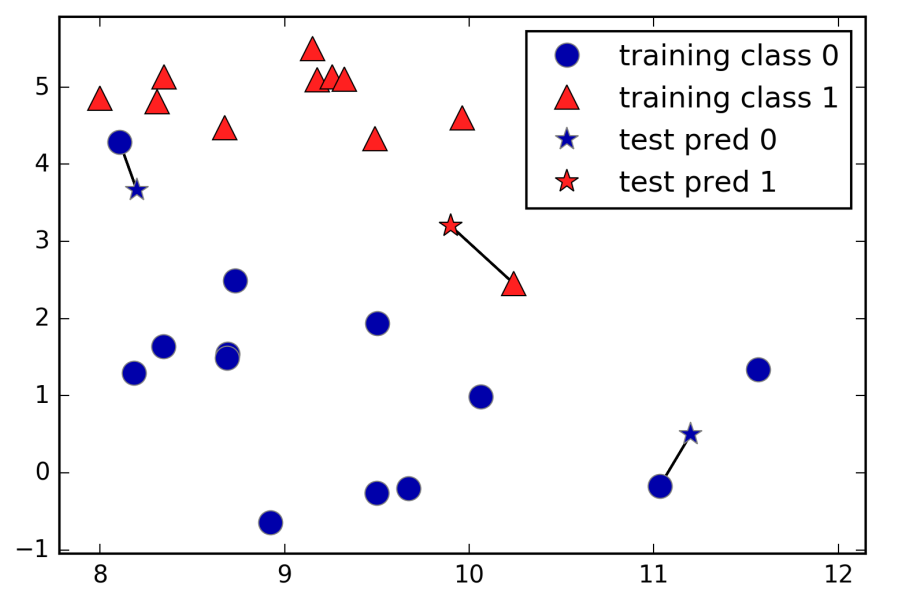
\includegraphics[scale=0.50]{../Imagen_Machine/1-NN}
	\caption{La predicciones se hacen con el modelo de 1-NN sobre la data forge.}
	\label{1-NN}
\end{figure} 


También podemos considerar un número $k$  arbitrario vecinos, en lugar de considerar sólo un vecino más cercano,  de aquí  el nombre del algoritmo de k-vecinos más cercanos.
Cuando se considera más de un vecino, la técnica usa la frecuencia o votación para asignar la
etiqueta.  Esto significa que para cada punto de prueba, se cuenta cuántos vecinos pertenecen
a la clase 0 y cuántos vecinos pertenecen a la clase 1. Luego le asigna la clase con mayor frecuencia, en otras palabras, la clase mayoritaria entre los k-vecinos más cercanos. \\

El siguiente ejemplo (Figura \ref{3-NN}) emplea la técnica con 3-vecinos más cercanos:\\

\begin{lstlisting}
In[11]:  mglearn.plots.plot_knn_classification(n_neighbors=3)
\end{lstlisting}

\begin{figure}[h!]
	\centering
	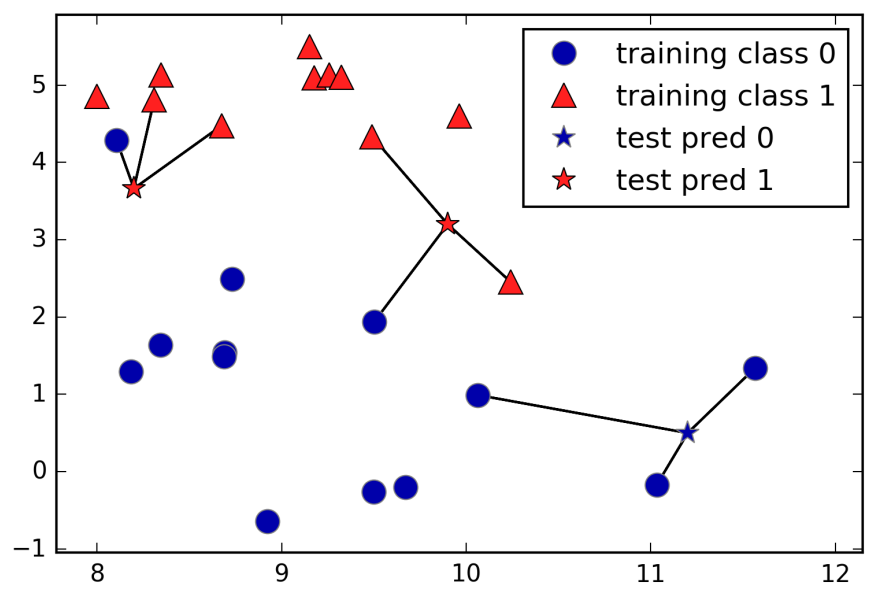
\includegraphics[scale=0.50]{../Imagen_Machine/3-NN}
	\caption{Predicciones hechas por el modelo 3-NN en la data falsificación de datos (forge dataset)}
	\label{3-NN}
\end{figure} 


Nuevamente, la predicción se muestra con el color de la estrella. Puedes ver que la predicción para el  punto nuevo  en la parte superior izquierda no es la misma que resultó  cuando
se  usó  un único vecino (1-NN).\\


Esta ilustración es corresponde al problema de clasificación binaria, pero el método  puede ser  
aplicado a conjuntos de datos con cualquier número de clases. En el caso de más de dos clases, es semejante, se cuentan  cuántos los vecinos pertenecen a cada clase y nuevamente predicen la clase más frecuente.\\



Ahora vemos cómo se aplicar el algoritmo k-vecinos más cercanos usando  {\ttfamily scikit-learn}. 
Primero, dividimos los datos en el conjunto de entrenamiento y el conjunto de prueba, necesario para  evaluar el rendimiento del modelo, como se discutió en el Capítulo \ref{Cap1}:\\


\begin{lstlisting}
In[12]:  from sklearn.model_selection import train_test_split
         X, y = mglearn.datasets.make_forge()
         
         X_train, X_test, y_train, y_test = train_test_split(     
                 X, y, random_state=0)
         
\end{lstlisting}


Seguidamente importamos e instanciamos la clase. Esto es cuando se establecen los parámetros, como el número de vecinos a usar, que en este caso es  3.\\

\begin{lstlisting}
In[13]:  from sklearn.neighbors import KNeighborsClassifier
         clf = KNeighborsClassifier(n_neighbors=3)
         
\end{lstlisting}


Ahora, ajustamos el clasificador sobre el conjunto de entrenamiento. Para el {\ttfamily KNeighboursClassifier}, significa almacenar el conjunto de datos, para  calcular los vecinos durante la predicción:\\

\begin{lstlisting}
In[14]:  clf.fit(X_train, y_train)

\end{lstlisting}

Para hacer la predición sobre la data de prueba, invocamos el método predictor. Para cada punto en el conjunto de prueba, este calcula su vecino más cercano en la data de entrenamiento, y calcula la clase más común entre estos. \\


\begin{lstlisting}
In[15]:  print("Predicciones en el conjunto de prueba: {}".format(
                 clf.predict(X_test)))

Out[15]: 

Predicciones en el conjunto de prueba: [1 0 1 0 1 0 0]

\end{lstlisting}


Para evaluar qué tan bien generaliza el modelo, podemos usar el método { \ttfamily {score }} aplicado a la data de prueba junto con sus etiquetas:\\

\begin{lstlisting}
In[16]:  print("Exactitud en el conjunto de prueba: {:.2f}".format(
                 clf.score(X_test, y_test)))

Out[16]:

    Exactitud en el conjunto de prueba: 0.86
\end{lstlisting}

Este resultado indica que el modelo es proximadamente 86\% exacto, esto significa que el modelo predice la clase correctamente para un  86\%  de las muestras en el conjunto de prueba.\\

 
Si bien esta ilustración es del problema de clasificación binaria, este método puede ser
aplicado a conjuntos de datos con cualquier número de clases. En el caso de  más clases, se cuenta  cuántos
los vecinos pertenecen a cada clase y nuevamente predicen la clase más común.\\


\subsubsection{Analizando KNeighboursClassifier}

Para conjuntos de datos bidimensionales, también podemos ilustrar la predicción para todos los  posibles puntos de prueba en el plano $XY$. Coloreando el área del plano de acuerdo con la clase que sería
asignado a un punto en esta región. Esto nos permite ver el límite de decisión donde el algoritmo asigna las clases, el cual es la división o límite entre las clases, en este caso   la clase 0  y  la clase 1.\\


El siguiente código produce la visualización del límite de decisión para uno, tres y nueve vecinos como se ve en la figura \ref{limites}.\\

\begin{lstlisting}
In[17]:  fig, axes = plt.subplots(1, 3, figsize=(10, 3))

         for n_neighbors, ax in zip([1, 3, 9], axes):
             # the fit method returns the object self, so 
             # we can instantiate  and fit in one line
             clf = KNeighborsClassifier(n_neighbors=n_neighbors).fit(X, y)
             mglearn.plots.plot_2d_separator(clf, X, fill=True, eps=0.5, 
                                              ax=ax, alpha=.4)
             mglearn.discrete_scatter(X[:, 0], X[:, 1], y, ax=ax)
             ax.set_title("{} neighbor(s)".format(n_neighbors))
             ax.set_xlabel("feature 0")
             ax.set_ylabel("feature 1")
         axes[0].legend(loc=3)

\end{lstlisting}

\begin{figure}[h!]
	\centering
	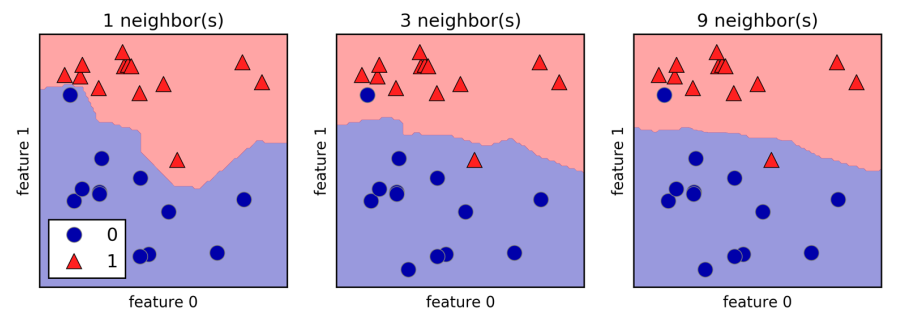
\includegraphics[scale=0.70]{../Imagen_Machine/limites}
	\caption{Límites de decisión creados por el modelo de vecinos más cercanos para diferentes valores
		de k-vecinos}
	\label{limites}
\end{figure} 

Como se ve a la izquierda en la figura \ref{limites}, usando un sólo vecino resulta  un límite de decisión
que sigue muy cercono  los datos de entrenamiento.  Considerando cada vez más vecinos conduce a un límite de decisión más suave. Un límite más suave corresponde a un modelo simple. En otras palabras, usar pocos vecinos corresponde a un modelo de alta complejidad (como se muestra en el lado derecho de la Figura \ref{complejidad}), y utilizando  muchos más vecinos responde a un modelo de baja complejidad (como se muestra en el lado izquierdo de la Figura \ref{complejidad}).  Si se considera el caso extremo donde el número de vecinos es igual al número datos del conjunto de entrenamiento, cada punto del conjunto de prueba tendría exactamente los mismos vecinos (todos puntos de entrenamiento) y todas las predicciones serían las mismas: la clase más frecuente en el conjunto de entrenamiento.\\



Para analizar y visualizar la relación entre la complejidad del modelo y la generalización discutida anteriormente, desarrollamos una práctica sobre la data  real Cáncer de Mamas. Comencemos dividiendo la data en los dos conjuntos, el de entrenamiento y el de prueba. Luego evaluamos el rendimiento del conjunto  entrenamiento y  pruebas con diferentes números de vecinos. El resultado se muestra en la figura \ref{constraste_E_P}:\\

\begin{lstlisting}
In[18]:  from sklearn.datasets import load_breast_cancer

         cancer = load_breast_cancer()
         X_train, X_test, y_train, y_test = train_test_split(
             cancer.data, cancer.target, stratify=cancer.target,
             random_state=66)
         
         training_accuracy = []
         test_accuracy = []
         # try n_neighbors from 1 to 10
         neighbors_settings = range(1, 11)
         
         for n_neighbors in neighbors_settings:
         # build the model
             clf = KNeighborsClassifier(n_neighbors=n_neighbors)
             clf.fit(X_train, y_train)
             # record training set accuracy
             training_accuracy.append(clf.score(X_train, y_train))
             # record generalization accuracy
             test_accuracy.append(clf.score(X_test, y_test))
             
         
         plt.plot(neighbors_settings, training_accuracy,
                  label="training accuracy")
         plt.plot(neighbors_settings, test_accuracy, 
                  label="test accuracy")
         plt.ylabel("Accuracy")
         plt.xlabel("n_neighbors")
         plt.legend()
\end{lstlisting}

\begin{figure}[h!]
	\centering
	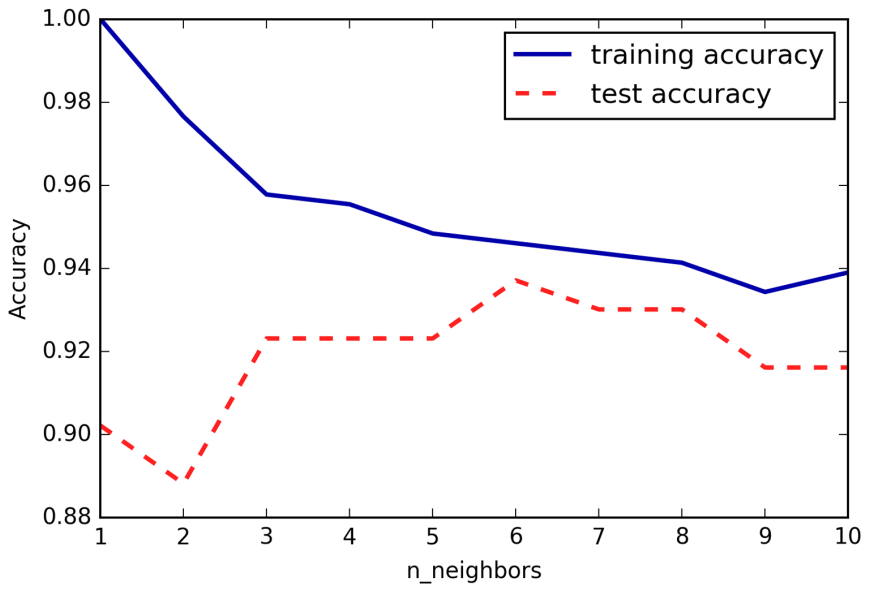
\includegraphics[scale=0.50]{../Imagen_Machine/constraste_E_P}
	\caption{Comparación de la exactitud en data entrenamiento y prueba con una función { \ttfamily   	 {}n\_neighbours}  }
	\label{constraste_E_P}
\end{figure} 


El gráfico muestra la exactitud en el conjunto de entrenamiento y  prueba en el eje $y$ contra la configuración del k-vecino sobre el eje $x$.  Los graficos del mundo real rara vez son suaves o muy suaves, sin embargo, podemos reconocer algunas de las características de sobreajuste y falta de ajuste (recuerde  que considerando pocos vecinos el modelo se hace más complejo). Considerando un único vecino más cercano, la predicción en el conjunto de entrenamiento es perfecta. Pero cuando  se consideran más vecinos, el modelo se vuelve más simple y la exactitud del entrenamiento disminuye. La exactitud del conjunto de prueba para  un solo vecino es menor que cuando se usan más vecinos, lo que indica que usar un solo vecino más cercano conduce a un modelo que es demasiado complejo. Por otro lado, cuando se consideran 10 vecinos, el modelo es demasiado simple, y el rendimiento es aún peor.   

El mejor rendimiento está en algún lugar intermedio, como 
alrededor de seis vecinos. Aún así, es bueno tener en cuenta la escala del gráfico. El peor rendimiento es alrededor del 88\%  de exactitud, lo que aún podría ser aceptable.\\


\subsubsection{Regresión con k-vecinos}

También hay una variante de regresión del algoritmo del  k-vecinos\index{regresión k-vecinos más cercano} más cercanos. Para ilustrar esta técnica se usará el conjunto de datos de Onda (wave). La técnica  se empieza a implementar  con un sólo vecino, y  se agregaron tres puntos de prueba representados como estrellas verdes en el eje $x$. La predicción usando un solo vecino que es el valor objetivo del vecino más cercano. Estos se muestran como estrellas azules en la Figura \ref{regresionPresicion}:\\

\begin{lstlisting}
In[19]:  mglearn.plots.plot_knn_regression(n_neighbors=1)

\end{lstlisting}

\begin{figure}[h!]
	\centering
	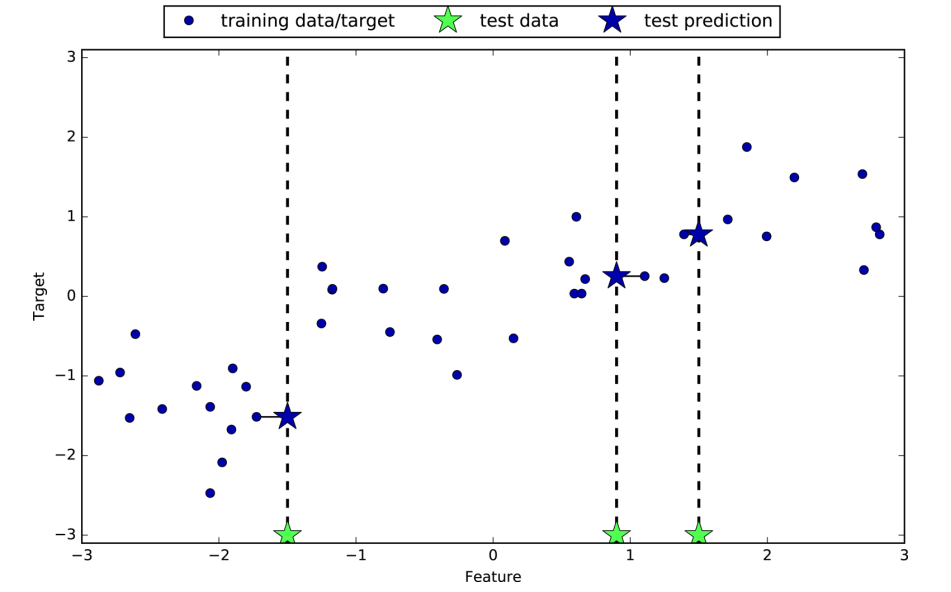
\includegraphics[scale=0.50]{../Imagen_Machine/regresionPresicion}
	\caption{Predicciones hechas por la regresión del vecino más cercano en el conjunto de datos de onda }
	\label{regresionPresicion}
\end{figure} 


Nuevamente, con esta técnica (regresión) también podemos usar más de un vecino, como el  caso de clasificación. Cuando se usa
múltiples vecinos, la predicción es el promedio o la media de los vecinos relevantes (Figura 2-9):\\

\begin{lstlisting}
In[20]:  mglearn.plots.plot_knn_regression(n_neighbors=3)

\end{lstlisting}

\begin{figure}[h!]
	\centering
	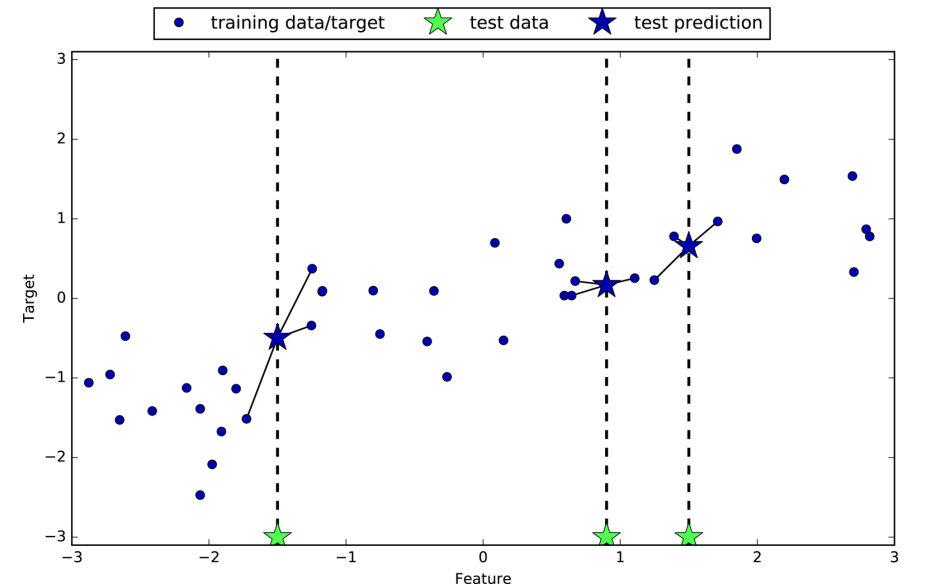
\includegraphics[scale=0.50]{../Imagen_Machine/Predicionregresion3}
	\caption{Predicciones hechas por la regresión de 3 vecinos en el conjunto de datos de onda}
	\label{Predicionregresion3}
\end{figure} 



El algoritmo del k-vecinos más cercanos para la regresión se implementa en la clase del regresor del  K-Neighbors  en {\ttfamily scikit-learn}. Se usa de manera similar a {\ttfamily KNeighboursClassifier}:\\


\begin{lstlisting}
In[21]:  from sklearn.neighbors import KNeighborsRegressor

         X, y = mglearn.datasets.make_wave(n_samples=40)
         
         # split the wave dataset into a training and a test set
         X_train, X_test, y_train, y_test = train_test_split(
                 X, y, random_state=0)

         # instantiate the model and set the number of neighbors 
         #  to consider to 3
         reg = KNeighborsRegressor(n_neighbors=3)
         # fit the model using the training data and training targets
         reg.fit(X_train, y_train)
\end{lstlisting}

\noindent y ahora  hacemos la predicción sobre el conjunto de prueba:\\ 

 
\begin{lstlisting}
In[22]:  print("Prediciones en el Conjuto de prueba:\n{}".format(
                 reg.predict(X_test)))

Out[22]:

   "Prediciones en el Conjuto de prueba:
   [-0.054 0.357 1.137 -1.894 -1.139 -1.631 0.357 0.912 -0.447 -1.139]
\end{lstlisting}


También podemos evaluar el modelo utilizando el método de score o puntuación, en el cual los regresores retornan  el puntaje de  $R^{2}$, también conocido como coeficiente de determinación, esta es una medidad
de la bondad de  predicción para un modelo de regresión, y da una puntuación entre 0
y 1. Un valor de 1 corresponde a una predicción perfecta, y un valor de 0 corresponde
a un modelo constante que solo predice la media de las respuestas del conjunto de entrenamiento {\ttfamily{ y\_train}}:\\


\begin{lstlisting}
In[23]:  print("R^2 en conjunto de Prueba: {:.2f}".format(
                 reg.score(X_test, y_test)))

Out[23]:
    R^2 en conjunto de Prueba: 0.83
   
\end{lstlisting}

Aquí, la puntuación es de 0,83, lo que indica un ajuste del modelo relativamente bueno.



\subsubsection{Analizando el KNeighborsRegressor}


Para la data unidimensional, podemos visualizar cómo se ven las predicciones para todos los valores 
posibles  de las características (Figura \ref{PredicionregresionMAS3}). Para hacer esto, creamos un conjunto  de prueba que consiste en muchos puntos sobre la línea:\\


\begin{lstlisting}
In[24]: fig, axes = plt.subplots(1, 3, figsize=(15, 4))
        # create 1,000 data points, evenly spaced between -3 and 3
        line = np.linspace(-3, 3, 1000).reshape(-1, 1)
        for n_neighbors, ax in zip([1, 3, 9], axes):
            # make predictions using 1, 3, or 9 neighbors
            reg = KNeighborsRegressor(n_neighbors=n_neighbors)
            reg.fit(X_train, y_train)
            ax.plot(line, reg.predict(line))
            ax.plot(X_train, y_train, '^', c=mglearn.cm2(0), markersize=8)
            ax.plot(X_test, y_test, 'v', c=mglearn.cm2(1), markersize=8)
			 
            ax.set_title(
               "{}neighbor(s)\n train score:{:.2f} test score:{:.2f}".format(
                  n_neighbors, reg.score(X_train, y_train),
                  reg.score(X_test, y_test)))
            ax.set_xlabel("Feature")
            ax.set_ylabel("Target")
        axes[0].legend(["Model predictions", "Training data/target",
                        "Test data/target"], loc="best")

\end{lstlisting}

\begin{figure}[h!]
	\centering
	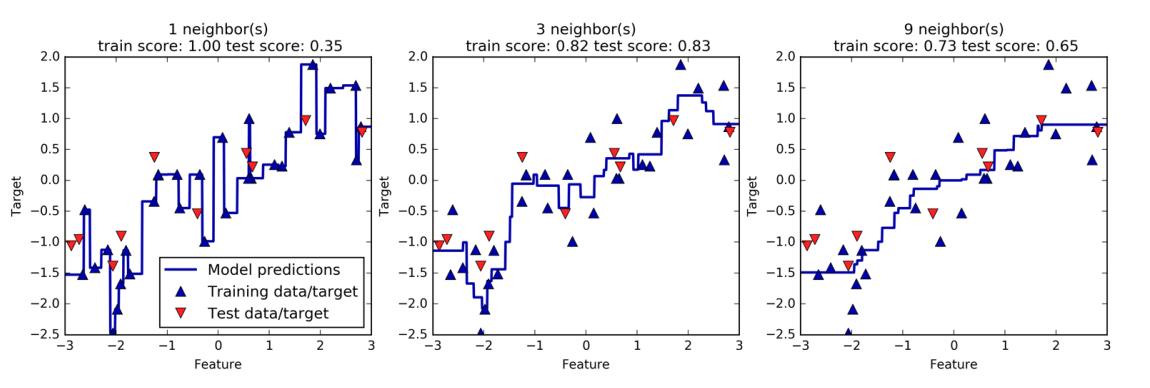
\includegraphics[scale=0.50]{../Imagen_Machine/PredicionregresionMAS3}
	\caption{ Comparando predicciones hechas con regresión del vecino más cercano para diferentes 
		valores de $k.$}
	\label{PredicionregresionMAS3}
\end{figure} 


Como podemos ver en el gráfico, usando un sólo vecino,  cada punto en el conjunto de entrenamiento tiene una influencia obvia en las predicciones,  y los valores predichos pasan por todos los puntos de datos.   Esto lleva a una predicción muy inestable.   Considerando más  vecinos conduce a predicciones más suaves,    pero estos no  se ajustan tan bien  a los datos de entrenamiento.


\subsubsection{Fortalezas, debilidades y parámetros}


En principio,  el clasificador  {\ttfamily KNeighbours} tiene  dos parámetros importantes: el
número de vecinos y la distancia (métrica) entre puntos de la data. En la práctica,
se usa un  número pequeño de vecinos, como tres o cinco que generalmete funciona bien, pero debe
ajustarse este parámetro. Seleccionar la métrica de distancia correcta, por ahora es algo que va 
más allá del alcance de este libro. Por defecto, se usa la distancia euclidiana, que funciona
bien en muchos entornos.\\


Una de las fortalezas de k-NN es que el modelo es muy fácil de entender, y a menudo
ofrece un rendimiento razonable sin muchos ajustes. Este algoritmo es un buen método de referencia para probar antes de considerar técnicas más avanzadas.\\

 
La construccón del modelo del vecinos más cercano suele ser muy rápido, pero cuando el conjunto de entrenamiento es muy grande (ya sea en número de características o en número de muestras)  la predicción puede ser lenta.  Cuando se utiliza el algoritmo k-NN, es importante preprocesar sus datos (consulte el Capítulo \ref{Cap3}).  Este enfoque generalmente no funciona bien sobre data con muchas características (cientos o más), y lo hace particularmente mal en conjuntos de datos donde la mayoría de las características son cero  en su mayor parte de las veces (los llamados conjuntos de datos dispersos\index{conjuntos dispersos} o sparse\index{sparse}).\\



Así,  mientras  el algoritmo del k-vecinos más cercano es fácil de entender, en la práctica no es muy frecuente, debido a que la predicción es lenta y su incapacidad para manejar muchas características.
El método que discutimos a continuación supera estos inconvenientes.


\subsection{Modelos lineales}


Los modelos lineales\index{modelos lineales} son una clase de modelos usados ampliamente en la práctica y han sido extensamente estudiados  en las últimas décadas, sus raíces que se remontan a más de cien
años. Los modelos lineales hacen una predicción usando una función lineal, donde la variable de entrada son las características. 

A continuación explicamos en forma breve esta ecuación matemáticas, y que tal vez te sientas familiarizado con la misma,  pues es  la ecuación  matemática básica de una línea recta. 


\subsubsection{Modelos lineales para regresión}


Para la regresión, la fórmula general de predicción  para un modelo lineal tiene el siguiente ecuación:
\[ \hat{y}  = w [0] * x[0] + w[1] * x[1] + ... + w[p] * x[p] + b \]
Aquí,  los entes $ x[0], ...,x[p]$ denota las características (en este ejemplo, el número de características es $p+1$), $w$ y $b$  son los parámetros del modelo que  aprenden, y $\hat{y}$  es 
la predicción que hace el modelo.\\

 Para un conjunto de datos con una sola característica, su ecuación se reduce a siguiente expresión:\\
\[ \hat{y} = w [0] * x [0] + b \]

\noindent  Aquí, $w [0]$  es la pendiente y $b$ es la ordenada en el origen (intercepto o corte con $y$). Para más características, $w$ contiene las pendientes a lo largo de cada eje de características. Alternativamente, puede pensar en la respuesta pronosticada como una suma ponderada de las características de entrada, con ponderaciones (que pueden ser negativos o positivos) dadas por las entradas de $w$.\\

Con  la siguiente instrucción aplicado sobre la data Onda  (conjunto de datos unidimensional), los parámetros $ w[0] $  y  $ b $  aprenden  y  conducen a la siguiente línea recta (ver Figura \ref{LineaR1}):\\

\begin{lstlisting}
In[25]:  mglearn.plots.plot_linear_regression_wave()

Out[25]:

    w[0]: 0.393906 b: -0.031804

\end{lstlisting}

\begin{figure}[h!]
	\centering
	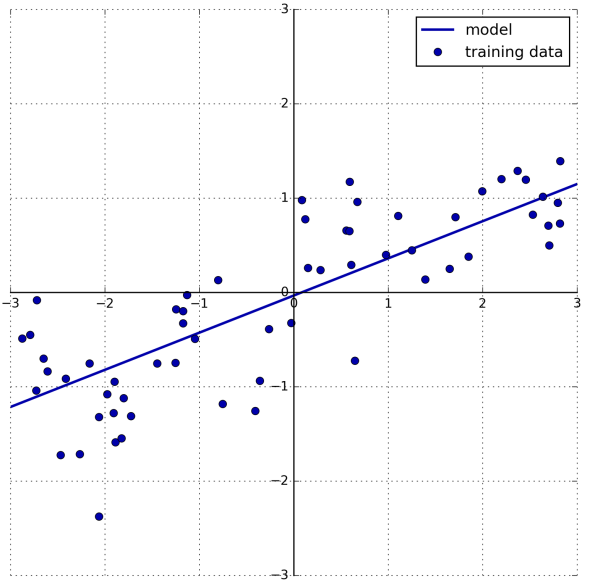
\includegraphics[scale=0.50]{../Imagen_Machine/LineaR1}
	\caption{Predicciones de un modelo lineal en el conjunto de datos de Onda}
	\label{LineaR1}
\end{figure} 



La pendiente  $ w[0],$ está al alrededor de 0.4, lo cual se puede confirmar 
visualizando el gráfico. La intersección es donde la línea de predicción corta el eje $y,$
está ligeramente por debajo de cero, lo que también se puede confirma en gráfico.\\

Los modelos de regresión lineal pueden caracterizarse como modelos de regresión para los cuales
la predicción es una línea cuando se trata de una sola característica, un plano  para dos características o un hiperplano para más de dos características  o alta dimensión (es decir, cuando se usan más características).\\

Si se compara las predicciones hechas por regresión lineal, con la técnica del  {\ttfamily KNeighboursRegressor} como se observa en  la figura \ref{PredicionregresionMAS3}, con la línea recta las predicciones son muy restringidas, y al parecer se pierden muchos de los detalles importantes de la data.  En cierto sentido, esto es cierto. Es una suposición fuerte (y poco  realista) que nuestro objetivo $y$,   es combinación lineal  de las características.  Para  datos con muchas características, los modelos lineales pueden ser muy potentes. En particular, si tiene más características que  datos de entrenamiento, cualquier objetivo $y$ puede ser perfectamente modelado como una función lineal (sobre el conjunto de entrenamiento). \\




Existen muchos modelos lineales diferentes para la regresión. La diferencia entre estos modelos radica en cómo  aprenden los parámetros $ w$  y  $b $   del modelo  en la data de entrenamiento, y cómo controlar la complejidad del modelo.

A continuación   revisaremos los  Modelos lineales más comunes  para la regresión.



 

\subsubsection{Regresión lineal}
% (también conocida como mínimos cuadrados ordinarios)

La regresión lineal o mínimos cuadrados ordinarios es el método más simple de regresión. La regresión lineal\index{regresión lineal} busca los parámetros $w$ y $b$ de tal manera que minimicen el error cuadrático medio  entre las predicciones $\hat{y},$  y los valores reales de la  regresión  $y,$ en el conjunto de entrenamiento. El error cuadrático medio es la suma de las diferencias al cuadrado entre las prediciones y los verdaderos valores. La regresión lineal no tiene parámetros a controlar, lo cual es un beneficio, pero pierde opción  de controlar la complejidad del modelo.\\

 
 
El código que se prensenta  a continuación  produce el modelo que se muestra en la Figura \ref{LineaR1}:\\

\begin{lstlisting}
In[26]:  from sklearn.linear_model import LinearRegression
         X, y = mglearn.datasets.make_wave(n_samples=60)
         X_train, X_test, y_train, y_test = train_test_split(
              X, y, random_state=42)
         
         lr = LinearRegression().fit(X_train, y_train)          

\end{lstlisting}

Los parámetros $w$ pendientes,  también  llamado ponderación o coeficiente, son almacenados en el atributo {\ttfamily lr.coef\_},  mientras que el intercepto $b$, es almacenado el atributo {\ttfamily intercept\_ }:\\


\begin{lstlisting}
In[27]:  print("lr.coef_: {}".format(lr.coef_))
         print("lr.intercept_: {}".format(lr.intercept_))

Out[27]:

    lr.coef_: [ 0.394]
    lr.intercept_: -0.031804343026759746

\end{lstlisting}
 
 
 
   

 
 \begin{minipage}[t]{0.2\textwidth}
 	\centering\raisebox{\dimexpr \topskip-\height}{%
 		
\includegraphics[width=\textwidth]{Imagen_Machine/Pajaro.png}}
 \end{minipage}%\hfill
 \begin{minipage}[t]{0.75\textwidth} 
 	{\scriptsize	
 	Observe el subrayado  final  de aspecto extraño (piso bajo después de coef e intercept) 		
 	al final  de {\ttfamily coef\_}  e  {\ttfamily intercepción\_}. El algoritmo {\ttfamily scikit-learn} siempre almacena cualquier   cosa que se  deriva de los datos de entrenamiento en atributos que terminan con un  subrayado final. Eso es para identificarlos de los parámetros que son establecidos por el usuario.}
 \end{minipage}\\


 El atributo intercepto es siempre un número float, mientras que el atributo {\ttfamily coef\_} es un arreglo NumPy con una entrada por característica. En el caso de la data Onda (wave) solo se tiene  una característica, así  el  coeficiente {\ttfamily lr.coef\_}   tiene  un sólo valor. \\


 Consideremos el rendimiento en el conjunto de entrenamiento y el de prueba: \\

\begin{lstlisting}
In[28]:  print("Training set score: {:.2f}".format(lr.score(
                  X_train, y_train)))
         print("Test set score: {:.2f}".format(lr.score(X_test, y_test)))

Out[28]:

   Training set score: 0.67
   Test set score: 0.66
   
\end{lstlisting}



Un $R^{2}$ cerca de 0.66 no es muy bueno, pero podemos ver que los puntajes de la data
entrenamiento y  prueba están muy cerca. Esto significa probablemente que tienen un subajuste, 
y no sobreajuste.  Para esta data unidimensional, existe poco peligro de sobreajuste, pues el modelo es muy simple (o restringido). Sin embargo, para data con alta dimensionalidad (data con gran número de características), el modelo de regresión es más potente, y existe alta probabilidad de sobreajuste. Veamos cómo se ejecuta  {\ttfamily LinearRegression} sobre una data más compleja, como la data  Boston Housing.
Recuerde que esta data  tiene 506 muestra y 105 características. Primero carguemos la data, y dividamos la data en dos, en data de entrenamiento y prueba. Luego construimos el modelo como antes:\\


\begin{lstlisting}
In[29]:  X, y = mglearn.datasets.load_extended_boston()
         X_train, X_test, y_train, y_test = train_test_split(
                 X, y, random_state=0)
         lr = LinearRegression().fit(X_train, y_train)
    
\end{lstlisting}     
         
Al comparar los puntajes del $R^{2}$ de la data entrenamiento con la de prueba, encontramos que la predicción en la data de entrenamiento es muy exacta (95\%), pero  en la data de prueba es aún más bajo (61\%):\\


\begin{lstlisting}
In[30]:  print("Training set score: {:.2f}".format(lr.score(
                 X_train, y_train)))
         print("Test set score: {:.2f}".format(lr.score(X_test, y_test)))

Out[30]:
 
    Training set score: 0.95
    Test set score: 0.61

\end{lstlisting}

Esta discrepancia de rendimiento en el conjunto de entrenamiento y  de prueba es una clara señal de sobreajuste; debido a esto debemos tratar de encontrar un modelo que nos permita controlar la complejidad. 


\subsubsection{Regression Ridge}


La regressión  Ridge\index{regressión  Ridge} es también un modelo de regresión,   por lo que la fórmula que  utiliza para las predicciones es misma que utilizan los modelos lineales bajo los mínimos cuadrados ordinarios. 
Aunque, en la regresión Ridge, los coeficientes $w$ están escogidos no sólo con el fin de que predigan bien en los datos de entrenamiento, sino  también para ajustar una restricción adicional; se trata que las magnitudes de los coeficientes sean lo más pequeño posible, en otras palabras, que todas las entradas de $w $ deberían estar próximas al cero.   Intuitivamente, esto quiere decir que cada característica debe tener poco efecto sobre el resultado en lo posible (esto significa que la pendiente debe ser pequeña), mientras  que el modelo siga prediciendo bien.  Esta restricción es un ejemplo de lo que es llamado regularización. La regularización\index{regularización} significa explícitamente restringir un modelo para evitar sobreajuste. El tipo  particular de regulación usada  por la regresión Ridge\index{regularización  $L2$} es conocida como Regularización  $L2$. \\

 La regresión Ridge está disponible  en  {\ttfamily scikit-learn}  como el modelo lineal  {\ttfamily linear\_model.Ridge}.   Veamos una aplicación de la regresión Ridge  sobre la data de Boston Housing y su rendimiento:\\


\begin{lstlisting}
In[31]:  from sklearn.linear_model import Ridge

         ridge = Ridge().fit(X_train, y_train)
         print("Training set score: {:.2f}".format(ridge.score(
                X_train, y_train)))
         print("Test set score: {:.2f}".format(ridge.score(
                X_test, y_test)))

Out[31]:
    
    Training set score: 0.89
    Test set score: 0.75

\end{lstlisting}
	
 
 Como se puede ver, el puntaje de la data de entrenamiento 0.89 es menor que la del modelo de {\ttfamily LinearRegression}  que resultó 0.95; mientras que el puntaje de la data de prueba es 0.75, resultado que supera el puntaje  del modelo {\ttfamily LinearRegression} con 0.61. Está situación es consistente con lo esperado; en el caso de regresión lineal con sobreajuste. Ridge es un modelo más restringido, así es que tenemos menos probabilidad de sobreajuste en el modelo.  Un modelo menos complejo quiere decir, menor rendimiento  sobre el conjunto de entrenamiento, pero mejora generalización. Como estamos  interesados sólo  en el rendimiento de generalización, deberíamos escoger el modelo Ridge en lugar del modelo regression lineal.\\
 

 El modelo  Ridge  hace una compensación (trade-off) entre la simplicidad del modelo (coeficientes cerca de cero) y su rendimiento sobre la data de entrenamiento. La mayor importancia del modelo es que coloca la simplicidad versus el rendimiento en la data entrenamiento, que puede ser especificada por el usuario, mediante el parámetro alfa. En el ejemplo anterior, se usó el parámetro {\ttfamily{alfa}} por defecto, esto es   {\ttfamily{alfa = 1}}. No hay razón para pensar qué esto siempre nos dará la mejor compensación; sin embargo, el ajuste óptimo del  {\ttfamily{alfa}} depende particularmente de la data que se use.  El incremento del {\ttfamily{alfa}} obliga a los coeficientes moverse más hacia el cero, lo cual decrese el rendimiento en la data de entrenamiento,  pero podría ayudar a la generalización. Por ejemplo:\\


\begin{lstlisting}
In[32]:  ridge10 = Ridge(alpha=10).fit(X_train, y_train)
         print("Training set score: {:.2f}".format(ridge10.score(
                X_train, y_train)))
         print("Test set score: {:.2f}".format(ridge10.score(
                X_test, y_test)))

Out[32]:
    
    Training set score: 0.79
    Test set score: 0.64

\end{lstlisting}

Disminuyendo el {\ttfamily{alfa}}, la  restricción es menor sobre los coeficientes, indicando que nos movemos a la derecha en de la Figura \ref{complejidad}. Para los valores muy pequeños de {\ttfamily{alfa}}, los coeficientes están restringidos del todo, y finalizamos con un modelo que se parece al modelo de regresión lineal (LinearRegression):\\


\begin{lstlisting}
In[33]:  ridge01 = Ridge(alpha=0.1).fit(X_train, y_train)
         print("Training set score: {:.2f}".format(
                 ridge01.score(X_train, y_train)))
         print("Test set score: {:.2f}".format(
                 ridge01.score(X_test, y_test)))

Out[33]:

    Training set score: 0.93
    Test set score: 0.77

\end{lstlisting}

En este caso el parámetro  {\ttfamily{alfa = 0.1}} parece trabajar bien. Podríamos probar disminuiyendo {\ttfamily{alfa}} un poco más para verificar si mejora la generalización. Por ahora, observe  cómo el parámetro {\ttfamily{alfa}} concuerda con la complejidad modelo, como se muestra en la Figura \ref{complejidad}. En el Capítulo \ref{Cap5} discutiremos el método para seleccionar los parámetros.\\ 


También podemos obtener una visión cualitativa  de cómo el parámetro {\ttfamily{alfa}} cambia el
modelo, observando el atributo {\ttfamily{coef\_}}  de modelos con diferentes valores de {\ttfamily{alfa}}. Un {\ttfamily{alfa}} alto significa un modelo más restringido; de esta forma, se espera que el  valor del {\ttfamily{coef\_}} tengan magnitud más pequeña para un valor alto de {\ttfamily{alfa}}, que para un valor bajo de {\ttfamily{alfa}}.  Esto se confirma en  el gráfico de la Figura \ref{alfa}:\\


\begin{lstlisting}
In[34]:  plt.plot(ridge.coef_, 's', label="Ridge alpha=1")
         plt.plot(ridge10.coef_, '^', label="Ridge alpha=10")
         plt.plot(ridge01.coef_, 'v', label="Ridge alpha=0.1")
         
         plt.plot(lr.coef_, 'o', label="LinearRegression")
         plt.xlabel("Coefficient index")
         plt.ylabel("Coefficient magnitude")
         plt.hlines(0, 0, len(lr.coef_))
         plt.ylim(-25, 25)
         plt.legend()

\end{lstlisting}



\begin{figure}[h!]
	\centering
	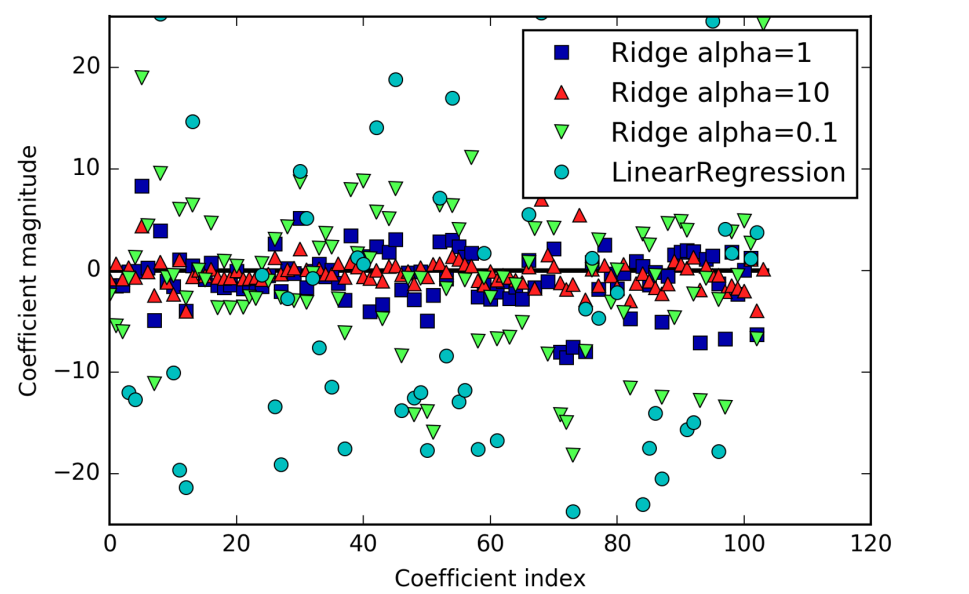
\includegraphics[scale=0.50]{../Imagen_Machine/alfa}
	\caption{Comparando las magnitudes de los coeficientes de la regresión de Ridge con los diferentes valores de alfa y la regresion lineal}
	\label{alfa}
\end{figure} 



Aquí, el eje $x$ enumera las entradas de {\ttfamily{coef\_:}}  $x = 0$  muestra el coeficiente asociado con la primera característica, $x = 1$ el coeficiente asociado con la segunda característica, y así sucesivamente hasta $x = 100$. El eje $y$ muestra los valores numéricos correspondientes a los
coeficientes. En este caso, la conclusión principal  es que para {\ttfamily{alfa = 10}}, los coeficientes se encuentran alrededor de $ {-}3$ y $3$. Los coeficientes del modelo Ridge con {\ttfamily{alfa = 1}} son un poco más grande. Y para  {\ttfamily{alfa = 0.1}} tienen una magnitud aún mayor, que el caso de la regresión lineal sin  regularización alguna (que sería alfa = 0), los coeficientes son tan grandes que están fuera del gráfico.\\


Otra forma de entender la influencia de la regularización es fijar un valor de alfa
y variar la cantidad de datos de entrenamiento disponibles. Con la data Boston Housing  ilustremos está situación; se ejecuta un proceso  sub-muestreo  en la data,  luego se evaluan las técnicas {\ttfamily LinearRegression} y {\ttfamily  Ridge(alpha = 1)}, incrementando los tamaño del conjunto de entrenamiento, el resultado se muestra en la figura \ref{RigiLineal}, los gráficos muestran el rendimiento del modelo en función del tamaño de datos, y se llaman curvas de aprendizaje:\\

\begin{lstlisting}
In[35]:  mglearn.plots.plot_ridge_n_samples()

\end{lstlisting}

\begin{figure}[h!]
	\centering
	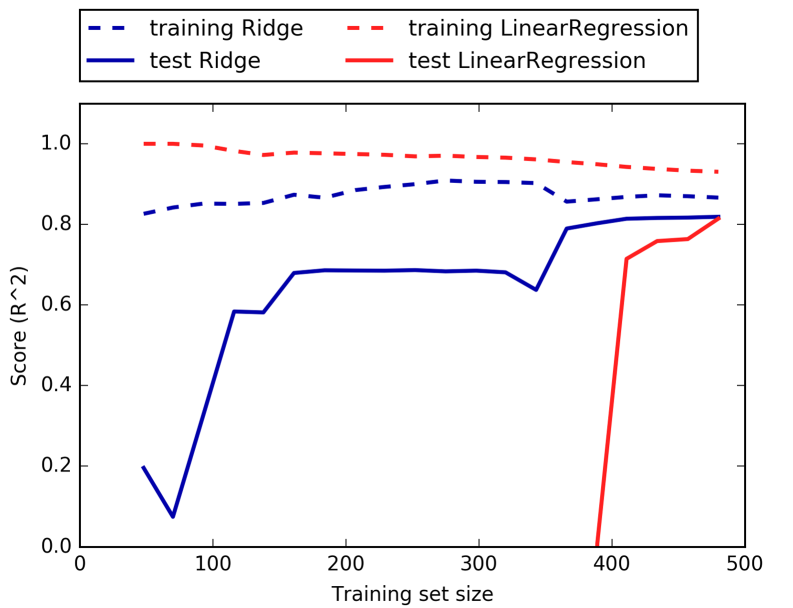
\includegraphics[scale=0.50]{../Imagen_Machine/RigiLineal}
	\caption{Comparando las magnitudes de los coeficientes de la regresión de Ridge con los diferentes valores de {\ttfamily{alfa}} y la regresion lineal}
	\label{RigiLineal}
\end{figure} 


Como era de esperar, el puntaje (score)  en la data entrenamiento es más alto que en la data de prueba en todos  tamaños de muestra, tanto para Ridge como en regresión lineal.  Debido a que Ridge está regularizada, el puntaje de la data de entrenamiento con Ridge  es menor que el puntaje de la data de entrenamiento con la regresión lineal en todos los ámbitos. Sin embargo, el puntaje de la data de prueba en Ridge es mejor que la linenl, particularmente para subconjuntos  pequeños de datos. Para data con  menos de 400 puntos, la regresión lineal no es capaz de aprender nada.   Con más y  más datos  disponibles para el modelo, ambos modelos mejoran y la  regresión lineal se pone al día con la Ridgea al final (asintótico). La lección aquí es que con suficientes datos de entrenamiento, la regularización se vuelve menos importante; y con suficientes datos, la regresión Ridge  y la regresión lineal tendrán el mismo rendimiento (el hecho de que esto suceda aquí cuando se usa el conjunto de datos completo es solo por casualida). Otro aspecto interesante de la Figura \ref{RigiLineal} es la disminución del rendimiento de data de entrenamiento en la regresión lineal.  Si se agregan más datos,  disminuye la posibilidad de sobreajuste del modelo  o  se le hace más dificil al modelo memorizar los datos de entrenamiento.\\

   
\subsubsection{Lasso}

 Una alternativa a la técnica de regresión lineal de Ridge con regularización es Lasso\index{regresión Lasso}. Como sucede con la regresión Ridge,  Lasso usa también una restrinción sobre los coeficientes 
 llevandolos  cerca de cero, pero en una forma ligeramente diferente, la llamada regularización\index{regularización $L1$} $L1.$ La consecuencia de la regularización $L1$ es que cuando se usa la regresión Lasso, algunos coeficientes son exactamente cero. Esto significa que algunas características son  completamente  ignoradas por el modelo; y  puede  interpretarse como una forma de selección automático de las características.   Teniendo algunos coeficientes exactamente igual a cero el modelo se hace  más fácil de interpretar y además  puede revelar las características más importantes del modelo.\\
  
	Apliquemos la técnica de Lasso al conjunto de datos de Boston Housing:\\

\begin{lstlisting}

In[36]:  from sklearn.linear_model import Lasso

         lasso = Lasso().fit(X_train, y_train)
         print("Training set score: {:.2f}".format(
                lasso.score(X_train, y_train)))
         print("Test set score: {:.2f}".format(
                lasso.score(X_test, y_test)))
         print("Number of features used: {}".format(
                np.sum(lasso.coef_ != 0)))

Out[36]:

    Training set score: 0.29
    Test set score: 0.21
    Number of features used: 4
\end{lstlisting}

Como puede ver, el rendimiento de Lasso es muy malo, tanto  en el conjunto de entrenamiento como en el de prueba. Esto indica que esta subajustado, además solo usó 4 de las 105 características.
De manera similar a Ridge, Lasso también tiene un parámetro de regularización, {\ttfamily alfa}, que controla
 qué tan fuerte se llevan los coeficientes a cero.  En el ejemplo anterior, utilizamos el valor por defecto  {\ttfamily{alpha = 1.0}}. Para reducir la falta ajuste o subajuste,  disminuimos el  {\ttfamily alfa}  y probamos. Para disminuirlo  aumentamos el número máximo de iteraciones para ejecutarlo, configurando  el atributo  {\ttfamily max\_iter}:\\


\begin{lstlisting}
In[37]:  # Aumentando la configuracion predeterminada "max_iter", de lo
         # contrario, el modelo advertiria que debemos aumentar max_iter.
         lasso001 = Lasso(alpha=0.01, max_iter=100000).fit(
                        X_train, y_train)
         print("Training set score: {:.2f}".format(
                lasso001.score(X_train, y_train)))
         print("Test set score: {:.2f}".format(
                lasso001.score(X_test, y_test)))
         print("Number of features used: {}".format(
                np.sum(lasso001.coef_ != 0)))
Out[37]:

    Training set score: 0.90
    Test set score: 0.77
    Number of features used: 33

\end{lstlisting}



Un {\ttfamily alfa} bajo permite ajustar un modelo más complejo, el cual trabaja mejor sobre la data de entrenamiento  y prueba. El rendimiento es ligeramente mejor que la Ridge, y además usa $ 33$ características de las $105$. Esto hace el modelo más potente y fácil de entender.\\

Sin embargo, si configuramos un {\ttfamily alfa} demasiado bajo, nuevamente eliminamos el efecto de regularización y terminamos con sobreajuste, con un resultado similar a LinearRegression:\\

\begin{lstlisting}
In[38]:  lasso00001 = Lasso(alpha=0.0001, max_iter=100000).fit(
                          X_train, y_train)
         print("Training set score: {:.2f}".format(lasso00001.score(
                 X_train, y_train)))
         print("Test set score: {:.2f}".format(lasso00001.score(
                 X_test, y_test)))
         print("Number of features used: {}".format(
                np.sum(lasso00001.coef_ != 0)))

Out[38]:

    Training set score: 0.95
    Test set score: 0.64
    Number of features used: 94
\end{lstlisting}
           
   
 
 Nuevamente, podemos graficar los coeficientes de los diferentes modelos, similarmente como se obseva en la figura \ref{RigiLineal}. El resultado se muestra en la figura \ref{LasoRigi}.\\
 
 
\begin{lstlisting}
In[39]:  plt.plot(lasso.coef_, 's', label="Lasso alpha=1")
         plt.plot(lasso001.coef_, '^', label="Lasso alpha=0.01")
         plt.plot(lasso00001.coef_, 'v', label="Lasso alpha=0.0001")
         plt.plot(ridge01.coef_, 'o', label="Ridge alpha=0.1")
         plt.legend(ncol=2, loc=(0, 1.05))
         plt.ylim(-25, 25)
         plt.xlabel("Coefficient index")
         plt.ylabel("Coefficient magnitude")
\end{lstlisting}

\begin{figure}[h!]
	\centering
	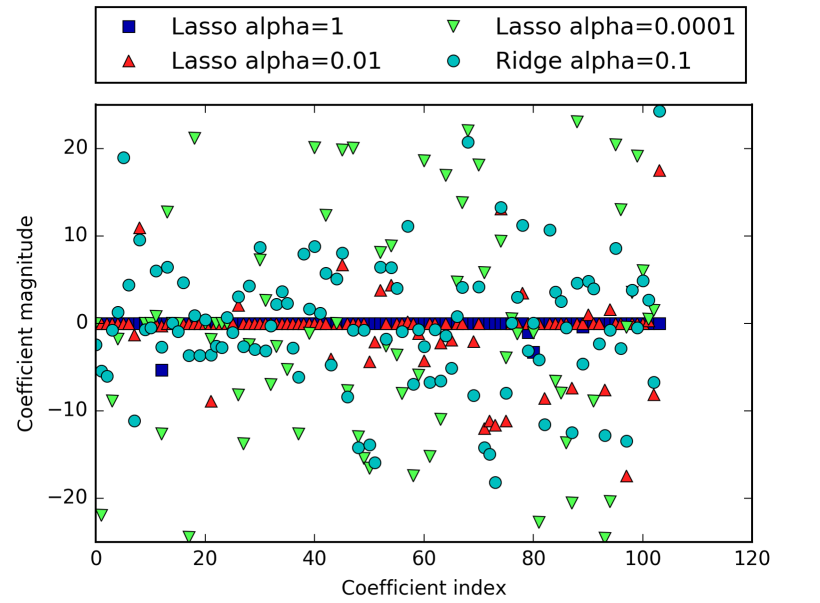
\includegraphics[scale=0.50]{../Imagen_Machine/LasoRigi}
	\caption{Comparación de las magnitudes de los coeficientes para la regresión de Lazo con diferentes valores  alfa y regresión Ridge}
	\label{LasoRigi}
\end{figure} 


Para   {\ttfamily{alfa = 1}}, no solo vemos que la mayoría de los coeficientes son cero (que ya conocíamos), sino que que los coeficientes restantes también son pequeños en magnitud. Llevando el  {\ttfamily{alfa = 0.01}}, obtenemos la solución que se muestra como los puntos rojos, lo que causa que la mayoría de las características son exactamente cero. Usando alfa = 0.00001, obtenemos un modelo poco regularizado, con la mayoría de los coeficientes distintos de cero y de gran magnitud.  Por comparación, la mejor solución de Ridge se muestra en verde azulado. El modelo Ridge con  {\ttfamily{alfa = 0.1}} tiene similar rendimiento predictivo al modelo de Lazo con  {\ttfamily{alfa = 0.01}}, pero usando Ridge, todos los coeficientes  son distintos de cero.\\

En la práctica, la regresión de Ridge suele ser la primera opción entre estos dos modelos.
Sin embargo, si tiene una gran cantidad de características y espera que solo unas pocas sean
importante, Lasso podría ser una mejor opción. Del mismo modo, si desea tener un modelo que sea más fácil de interpretar, Lasso proporcionará un modelo que es más fácil para interpretar y entender, ya que seleccionará solo un subconjunto de las características de entrada.  

scikit-learn también proporciona la clase ElasticNet, que combina las penalizaciones de Lasso y Ridge.  En la práctica, esta combinación funciona mejor, aunque al costo de tener dos parámetros para ajustar: uno para la regularización $L1$ y otro para la regularización $L2$.
 
\subsubsection{Modelos lineales para clasificación binaria}\label{Mlineales}

Los modelos lineales también se utilizan ampliamente para la clasificación. Consideremos la clasificación  binaria\index{clasificación  binaria}  en primer lugar. En este caso,  una predicción  se hace  utilizando la siguiente fórmula:

\[ \hat{y} = w[0] * x[0] +w[1] * x[1] + ... + w[p] * x [p] + b > 0  \]

La fórmula se ve muy similar a la de la regresión lineal, pero en lugar de 
retornar solo la suma ponderada de las características, limitamos el valor predicho a cero.  Si la función es menor que cero, predecimos la clase –1; si es mayor que cero, 
predecimos la clase +1. Esta regla de predicción es común a todos los modelos lineales para clasificación\index{Modelos lineales para clasificación}.
 Una vez más, hay varias formas diferentes de encontrar los coeficientes $w$ y el intercepto $b$.\\


Para los modelos lineales por regresión la salida  $\hat{y}$, es una función lineal de las características: una línea, un plano o un hiperplano (para dimensiones superiores). Para modelos lineales por clasificación, el límite de decisión es una función lineal de la entrada. En otras palabras, un clasificador lineal (binario) es el clasificador  que separa dos clases usando una línea, un plano o un hiperplano. Se ilustrará este clasificador con ejemplos más adelante a fin de aclara la situación. \\

Existen muchos algoritmos de aprendizaje automático con modelos lineales. Todos estos algoritmos difieren en las siguientes dos formas:

\begin{itemize}
	\item La forma en que miden qué tan bien la  combinación particular de coeficientes 
	e intercepto, se ajusta a los datos de entrenamiento
	
	\item Y qué tipo de regularización emplea
\end{itemize}


Los algoritmos eligen diferentes formas para medir qué "tan bien se ajustan a la data de entrenamiento".   Por razones matemáticas no es posible ajustar los parámetros $w$ y $b$, para minimizar la cantidad de clasificaciones erróneas que producen los algoritmos. Para nuestros propósitos y muchas aplicaciones, las diferentes opciones para el primer item  de la lista anterior tiene poca importancia  o significancia, y se conocen como  funciones de pérdida.


Los dos algoritmos de clasificación lineal más comunes son la regresión logística\index{regresión logística},  implementada
en  {\ttfamily{linear\_model.LogisticRegression}} y  máquinas de soporte de vectores lineal\index{máquinas de soporte de vectores lineal} (SVM lineales), implementado en {\ttfamily{svm.LinearSVC}} (SVC significa máquina de vector de soporte para clasificación).  A pesar de su nombre, LogisticRegression  es un algoritmo de clasificación y no un
algoritmo de regresión, y no debe confundirse con LinearRegression.\\


A continuaciónn se aplica los modelos {\ttfamily LogisticRegression} y {\ttfamily LinearSVC} sobre la dataset de falsificación de datos (forge dataset), y se visualizar el límite de decisión como se presenta en los modelos lineales (Figura \ref{SVM}):


\begin{lstlisting}
In[40]:  from sklearn.linear_model import LogisticRegression
         from sklearn.svm import LinearSVC
         
         X, y = mglearn.datasets.make_forge()
         
         fig, axes = plt.subplots(1, 2, figsize=(10, 3))
         
         for model, ax in zip([LinearSVC(), LogisticRegression()], axes):
             clf = model.fit(X, y)
             mglearn.plots.plot_2d_separator(clf, X, fill=False, eps=0.5,
                                             ax=ax, alpha=.7)
             mglearn.discrete_scatter(X[:, 0], X[:, 1], y, ax=ax)
             ax.set_title("{}".format(clf.__class__.__name__))
             ax.set_xlabel("Feature 0")
             ax.set_ylabel("Feature 1")
         axes[0].legend()
\end{lstlisting}


\begin{figure}[h!]
	\centering
	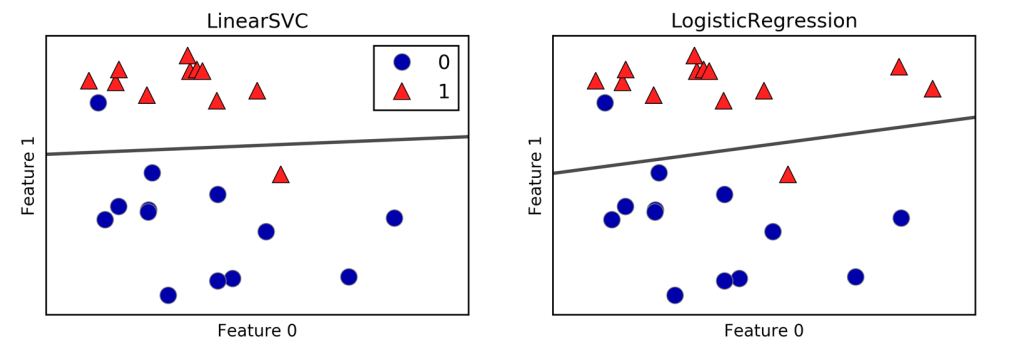
\includegraphics[scale=0.65]{../Imagen_Machine/SVM}
	\caption{Límites de decisión de la regresión lineal SVM  y regresión logística en la data falsificación de datos (forge dataset) con los parámetros por defecto}
	\label{SVM}
\end{figure}


% Figura 2-15. Límites de decisión de la regresión lineal SVM  y regresión logística en el conjunto de datos  forge con los parámetros por defecto.\\


En la figura \ref{SVM}, la primera característica de la  data de falsificación (forge dataset)  está en el eje $x,$   y la  segunda característica en el eje $y$. Se observan los límites de decisión encontrados por
LinearSVC y LogisticRegression respectivamente como líneas rectas, separando el área  clasificada como clase 1 en la parte superior, y como clase 0 en la parte inferior. En  otras palabras, cualquier dato nuevo que se encuentre por encima de la línea negra se clasificará como clase 1 por el clasificador respectivo, mientras que cualquier punto que se encuentre debajo de la línea negra se clasificará  como clase 0.\\

Los dos modelos presentan límites de decisión similares. Observe que ambos modelos clasifican erróneamente dos  puntos. Por defecto, ambos modelos aplican una regularización $L2$, en la misma
forma en que Ridge lo hace para la regresión.\\

Para LogisticRegression y LinearSVC, el parámetro de compensación (trade-off) que determina 
la regulaión se llama $C$. Para valores  altos de $C$ corresponden a menor regularización.
En otras palabras, cuando se usa un valor alto para el parámetro $C$, LogisticRegression y LinearSVC intentan ajustar el conjunto de entrenamiento lo mejor posible, mientras que con valores bajos de $C$, los modelos ponen más énfasis en encontrar un coeficiente $w$ que esté cerca de cero.\\


Hay otro aspecto interesante de cómo actúa el parámetro $C$. Usando valores bajos de $C$  hará que los algoritmos intenten ajustarse a la "mayoría" de los puntos de datos, mientras usan  un valor más alto de $C$, enfatiza la importancia de cada punto  individual de los datos sea clasificado correctamente. \\

A continuación se ilustra con la técnica  LinearSVC (Figura \ref{LinearSVC}):\\

\begin{lstlisting}
In[41]:  mglearn.plots.plot_linear_svc_regularization()

\end{lstlisting}

\begin{figure}[h!]
	\centering
	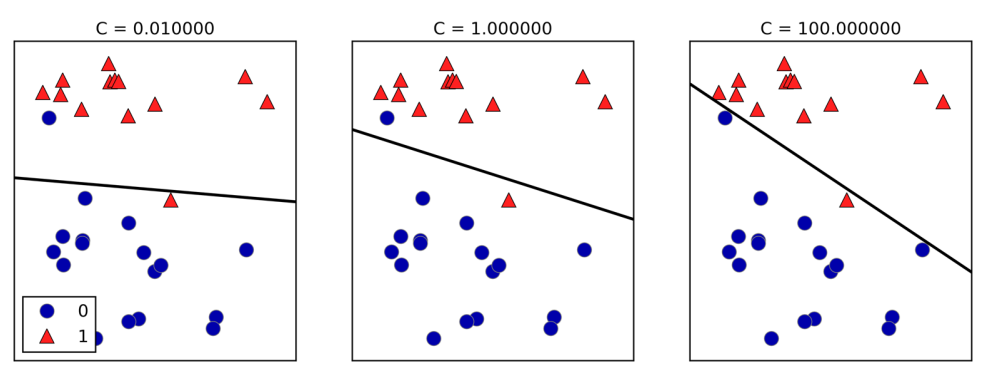
\includegraphics[scale=0.65]{../Imagen_Machine/LinearSVC}
	\caption{Límites de decisión de un SVM lineal en la data falsificación de datos (forge dataset) para diferentes valores de C}
	\label{LinearSVC}
\end{figure}


 En el lado izquierdo de la figura \ref{LinearSVC}, tenemos una $C$ muy pequeña que corresponde a una gran regularización. La mayoría de los puntos en la clase 0 se observan en la parte superior, igualmente que la mayoría de los puntos de la clase 1 están en la parte el inferior. El modelo fuertemente regularizado selecciona una línea relativamente horizontal, clasificando erróneamente dos puntos. En el grafico central, C es ligeramente más alto, el modelo se enfoca más en las dos muestras mal clasificadas, inclinando el límite de decisión.  Finalmente, en el lado derecha, el valor muy alto de $C$, el modelo inclina aún más el límite de decisión, y ahora clasifica correctamente todos los puntos en la clase 0. Pero uno de los puntos en la clase 1 sigue siendo clasificado mal, ya que no es posible clasificar correctamente todos los puntos en este conjunto de datos usando una recta línea. El modelo ilustrado en el lado derecho se esfuerza por clasificar correctamente todos  puntos, pero podría no capturar bien el diseño general de las clases. En otras palabras,  es probable que este modelo esté sobreajustado.\\


De manera similar al caso de regresión, los modelos lineales para clasificación pueden parecer muy
restrictivo en espacios de baja dimensión, solo permitiendo límites de decisión que son
líneas rectas o planos.  Sin embargo,  en  altas dimensiones los modelos lineales para clasificación 
se vuelve muy poderoso, y la protección contra el sobreajuste se vuelve cada vez más importante al considerar más características.\\ 


Analicemos el algoritmo LinearLogistic con más cuidado con el conjunto de datos Cáncer de mama (Breast Cancer dataset):\\ 


\begin{lstlisting}
In[42]:  from sklearn.datasets import load_breast_cancer
         cancer = load_breast_cancer()
         X_train, X_test, y_train, y_test = train_test_split(cancer.data, 
              cancer.target, stratify=cancer.target, random_state=42)
         logreg = LogisticRegression().fit(X_train, y_train)
         print("Training set score: {:.3f}".format(
                logreg.score(X_train, y_train)))
         print("Test set score: {:.3f}".format(
                logreg.score(X_test, y_test)))
Out[42]:

    Training set score: 0.953
    Test set score: 0.958
\end{lstlisting}


El valor por defecto de $C$ es 1, y proporciona un buen rendimiento, con una exactitud del 95\% , tanto el conjunto de entrenamiento como en el de prueba. Pero como el rendimiento en el  conjunto entrenamiento y en el de pruebas son muy cercanos, es probable presente cierto  subajutes.  Aumentemos $C,$ para que se ajuste a una forma más flexible el modelo:\\


\begin{lstlisting}
In[43]:  logreg100 = LogisticRegression(C=100).fit(X_train, y_train)
         print("Training set score: {:.3f}".format(
                logreg100.score(X_train, y_train)))
         print("Test set score: {:.3f}".format(
                logreg100.score(X_test, y_test)))

Out[43]:

    Training set score: 0.972
    Test set score: 0.965
\end{lstlisting}

Usando un $C = 100,$ da como resultado una mayor exactitud del conjunto de entrenamiento y también un  ligero aumento en el de prueba,  confirmando nuestra intuición de que un modelo más complejo debería funcionar mejor. También podemos investigar qué sucede si utilizamos un modelo aún más regularizado que
el valor por defecto ($ C = 1$), configurando $C = 0.01$: \\

\begin{lstlisting}
In[44]:  logreg001 = LogisticRegression(C=0.01).fit(X_train, y_train)
         print("Training set score: {:.3f}".format(
                 logreg001.score(X_train, y_train)))
         print("Test set score: {:.3f}".format(
                 logreg001.score(X_test, y_test)))
Out[44]:

    Training set score: 0.934
    Test set score: 0.930
\end{lstlisting}

Como era de esperar, al moverse más a la izquierda a lo largo de la escala mostrada en la Figura \ref{complejidad}  resulta  un modelo  subajustado, tanto en el conjunto de entrenamiento y como en el de prueba, la exactitud disminuye en relación con los parámetros por defecto.\\


Finalmente, veamos los coeficientes aprendidos por los modelos con los tres conjuntos diferentes del parámetro de regularización $C$ (Figura \ref{Rlogistica}):\\

\begin{figure}[h!]
	\centering
	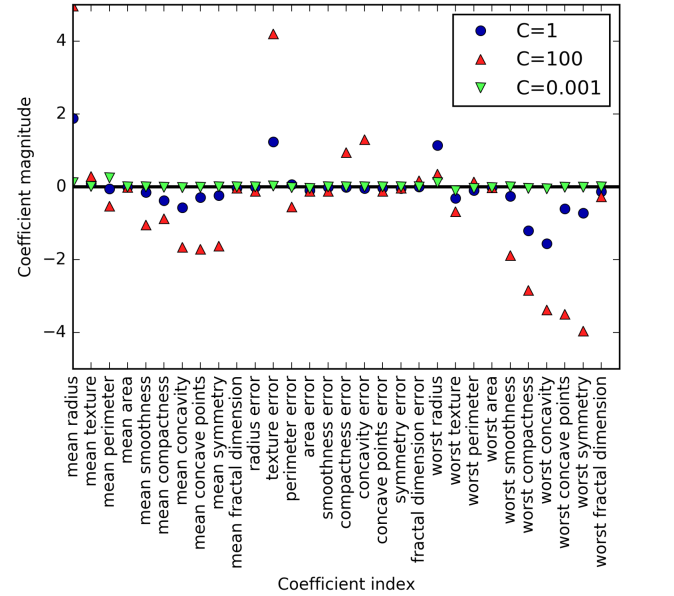
\includegraphics[scale=0.65]{../Imagen_Machine/Rlogistica}
	\caption{Coeficientes aprendidos por regresión logística en el conjunto de datos de Cáncer de Mama para
		diferentes valores de C}
	\label{Rlogistica}
\end{figure}

\begin{lstlisting}
In[45]:  plt.plot(logreg.coef_.T, 'o', label="C=1")
         plt.plot(logreg100.coef_.T, '^', label="C=100")
         plt.plot(logreg001.coef_.T, 'v', label="C=0.001")
         plt.xticks(range(
                cancer.data.shape[1]), cancer.feature_names, rotation=90)
         plt.hlines(0, 0, cancer.data.shape[1])
         plt.ylim(-5, 5)
         plt.xlabel("Coefficient index")
         plt.ylabel("Coefficient magnitude")
         plt.legend()

\end{lstlisting}

 


\begin{minipage}[t]{0.2\textwidth}
	\centering\raisebox{\dimexpr \topskip-\height}{%
		
\includegraphics[width=\textwidth]{Imagen_Machine/Escorpion.png}}
\end{minipage}%\hfill
\begin{minipage}[t]{0.75\textwidth} 
	{\scriptsize		
	Como la  {\ttfamily LogisticRegression} aplica una regularización $L2$ por defecto, el resultado parece similar  al producido por Ridge en la Figura \ref{RigiLineal}. Una regularización más fuerte obliga 
		a los coeficientes acercarse más hacia cero, aunque los coeficientes nunca llegan a ser 
		exactamente cero. Inspeccionando   el gráfico más de cerca, también podemos ver un efecto 
		interesante en el tercer  coeficiente,  para el   "{}perímetro medio"{}  \: (mean perimeter).   Para $C=100$ y $C=1$,
		el coeficiente es negativo, mientras que  para $C=0,001$, el coeficiente es positivo, con 
		una magnitud que es incluso mayor para  $C=1$. Interpretando un modelo como este, uno 
		podría  pensar que el coeficiente nos dice con qué clase se  asocia una característica. 
		Por ejemplo, uno podría pensar que un alto  valor en la característica "{}error de textura{}"{}   
		está relacionada con una muestra que es  "{}maligno."{}    \: Sin embargo, el cambio de signo en el 
		coeficiente de  "{}perímetro medio"{}  significa que dependiendo del modelo que miramos, un alto 
		{}"{}perímetro medio{}"{ }  podría ser tomado como  indicativo de "benigno"{ }  o indicativo de  "maligno". 	
	Esto ilustra que las interpretaciones de  coeficientes de modelos lineales siempre deben 	
	tomarse como gran cuidado.}
\end{minipage} \\


Si deseamos un modelo más interpretable, la regularización $L1$ podría ayudar, ya que límita al  modelo a utilizar sólo algunas características. \\

A continuación se presenta el gráfico de coeficientes y las precisiones de clasificación para tres regularizaciónes de $L1$,  0.001,  1  y  100  (Figure \ref{PenalRegreLogis}):\\




\begin{lstlisting}
In[46]:  for C, marker in zip([0.001, 1, 100], ['o', '^', 'v']):
             lr_l1 = LogisticRegression(C=C, penalty="l1").fit(
                                     X_train, y_train)
             print("Training accuracy of l1 logreg with C={:.3f}: {:.2f}"
                    .format(C, lr_l1.score(X_train, y_train)))
             print("Test accuracy of l1 logreg with C={:.3f}: {:.2f}".format(
                     C, lr_l1.score(X_test, y_test)))
             plt.plot(lr_l1.coef_.T, marker, label="C={:.3f}".format(C))
        
         plt.xticks(range(
                cancer.data.shape[1]), cancer.feature_names, rotation=90)
         plt.hlines(0, 0, cancer.data.shape[1])
         plt.xlabel("Coefficient index")
         plt.ylabel("Coefficient magnitude")
         
         plt.ylim(-5, 5)
         plt.legend(loc=3)

Out[46]:

	Training accuracy of l1 logreg with C=0.001: 0.91
	Test accuracy of l1 logreg with C=0.001: 0.92
	Training accuracy of l1 logreg with C=1.000: 0.96
	Test accuracy of l1 logreg with C=1.000: 0.96
	Training accuracy of l1 logreg with C=100.000: 0.99
	Test accuracy of l1 logreg with C=100.000: 0.98
\end{lstlisting}


Como pueden ver, hay muchos paralelismos entre los modelos lineales para la clasificación binaria y los modelos lineales para la regresión. Como en la regresión, la principal diferencia entre los modelos es el parámetro de penalización, que influye en la regularización y si el modelo utilizará todas las características disponibles o seleccionar sólo un subconjunto.\\


\begin{figure}[h!]
	\centering
	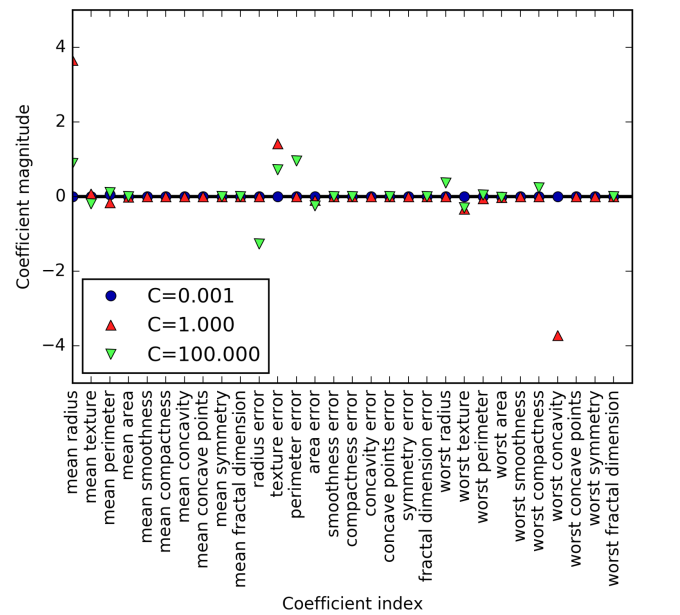
\includegraphics[scale=0.65]{../Imagen_Machine/PenalRegreLogis}
	\caption{Coeficientes aprendidos por regresión logística con penalización L1 en el Conjunto de datos sobre el cáncer para diferentes valores de C}
	\label{PenalRegreLogis}
\end{figure}




 \subsubsection{Modelos lineales para clasificación multiclases}
 %Linear models for multiclass classification

Muchos modelos de clasificación lineal son sólo para la clasificación binaria, y no se extienden naturalmente al caso multiclase (con la excepción de la regresión logística). Una técnica común para extender un algoritmo de clasificación binaria a un algoritmo de clasificación multiclase es el enfoque uno versus el resto (one-vs.-rest). En el enfoque one-vs.-rest, un modelo binario  es aprendido por cada clase que trata de separar esa clase de todas las otras clases, resultando  tantos modelos binarios como clases haya. Para hacer una predicción, todos los clasificadores binarios se ejecutan en un punto de prueba. El clasificador que tiene la puntuación (score) más alta en su única clase "gana", y esta  clase etiquetada  se devuelve como la predicción.\\

 

Tener un clasificador binario por cada clase, resulta también tener un vector de coeficientes $w$ y un intercepto $b$  para cada clase. La clase para la cual el resultado de la clasificación de la fórmula dada aquí, es la clase más alta a la que se le asigna la etiqueta:

\[  w [0] * x[0] + w[1] * x[1] + ... + w[p] * x[p] + b \]
 
 
Las matemáticas detrás de la regresión logística multiclase difieren un poco del enfoque uno versus el resto (one vs.-rest), pero también dan lugar a un vector de coeficiente e intercepto por clase, y se aplica el mismo método para predecir.\\

 
Ilustremos  el método one-vs.-rest para clasificar la data,  aplicado a un conjunto de datos  con tres clases. Es un conjunto de datos bidimensionales, donde cada clase viene dada por datos muestreados de una distribución gaussiana (ver Figura \ref{Toy} ): \\



\begin{lstlisting}
In[47]:  from sklearn.datasets import make_blobs

         X, y = make_blobs(random_state=42)
         mglearn.discrete_scatter(X[:, 0], X[:, 1], y)
         plt.xlabel("Feature 0")
         plt.ylabel("Feature 1")
         plt.legend(["Class 0", "Class 1", "Class 2"])
\end{lstlisting}



\begin{figure}[h!]
	\centering
	\includegraphics[scale=0.65]{../Imagen_Machine/Toy}
	\caption{Conjunto de datos bidimensional sobre juguetes que contiene tres clases}
	\label{Toy}
\end{figure}


Ahora, entrenemos  el classificador LinearSVC sobre la data:\\


\begin{lstlisting}
In[48]:  linear_svm = LinearSVC().fit(X, y)
         print("Coefficient shape: ", linear_svm.coef_.shape)
         print("Intercept shape: ", linear_svm.intercept_.shape)
Out[48]:

	Coefficient shape: (3, 2)
	Intercept shape: (3,)

\end{lstlisting}

Vemos que la forma del { \ttfamily coef\_} es (3, 2), lo que significa que cada fila de { \ttfamily coef\_}  contiene el vector de coeficientes para una de las tres clases y cada columna tiene el valor de coeficiente para una característica específica (hay dos en este conjunto de datos). El  { \ttfamily intercept\_}  es ahora una matriz unidimensional, almacenando los interceptos  para cada clase. \\

Visualizalicemos  las líneas de limites dadas por los tres clasificadores binarios (Figure \ref{3clases}):\\


\begin{lstlisting}
In[49]:  mglearn.discrete_scatter(X[:, 0], X[:, 1], y)
         line = np.linspace(-15, 15)
         for coef, intercept, color in zip(linear_svm.coef_, 
                                           linear_svm.intercept_,
                                           ['b', 'r', 'g']):
             plt.plot(line,
                      -(line * coef[0] + intercept) / coef[1], c=color)
         plt.ylim(-10, 15)
         plt.xlim(-10, 8)
         plt.xlabel("Feature 0")
         plt.ylabel("Feature 1")
         plt.legend(['Class 0', 'Class 1', 'Class 2','Line class 0', 
                     'Line class 1', 'Line class 2'], loc=(1.01, 0.3))
\end{lstlisting}


Se puede ver que todos los puntos pertenecientes a la clase 0 en los datos de entrenamiento están por encima de la línea correspondiente a la clase 0, lo que significa que están en el lado "{}clase 0{}"{}  de este clasificador binario. Los puntos de la clase 0 están por encima de la línea correspondiente a la clase 2, lo que significa que están clasificados como "{}resto" {}   por el clasificador binario de la clase 2.



\begin{figure}[h!]
	\centering
	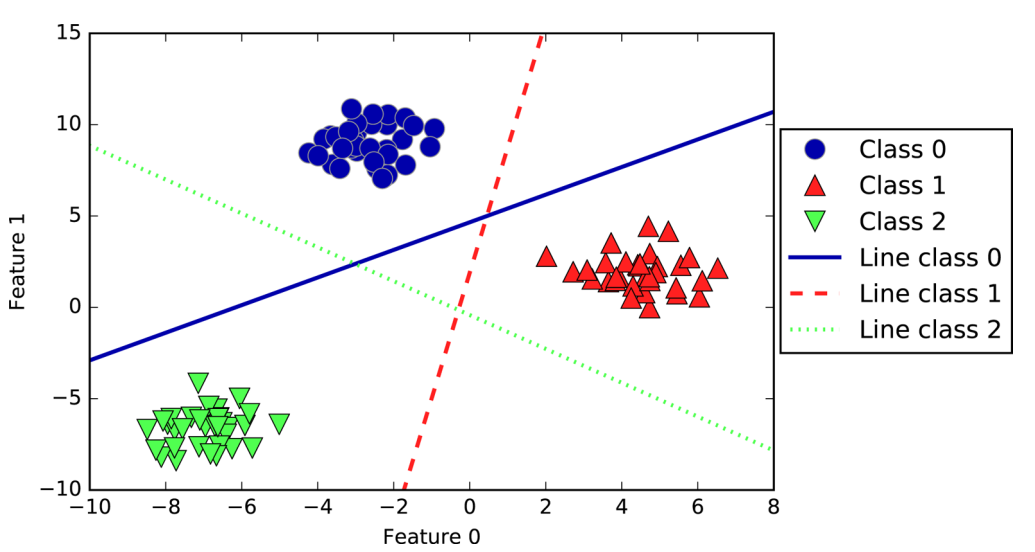
\includegraphics[scale=0.60]{../Imagen_Machine/3clases}
	\caption{Límites de decisión aprendidos por los tres clasificadores uno contra uno.-rest}
	\label{3clases}
\end{figure}

 \noindent Los puntos pertenecientes a la clase 0 que  están a la izquierda de la línea correspondiente a la clase 1,  lo que significa el clasificador binario para la clase 1 también los clasifica como "resto".  Por lo tanto, cualquier punto en esta área será clasificada como clase 0 por el clasificador final (el resultado de la fórmula de clasificación de confianza  para el clasificador "{}clase 0"{} es mayor que cero, mientras que es menor que cero para las otras dos clases).\\ 
 

¿Pero qué pasa con el triángulo en el centro del gráfico?   Los tres clasificadores binarios clasifican los puntos allí como "resto." ¿A qué clase se le asignaría un punto? La respuesta es la que tiene el valor más alto para la fórmula de clasificación: la clase de la línea más cercana.\\


El siguiente ejemplo (Figura \ref{2D}) muestra la predicción  para todas las regiones del espacio 2D:\\


\begin{lstlisting}
In[50]:  mglearn.plots.plot_2d_classification(linear_svm, X, 
                                               fill=True, alpha=.7)
         mglearn.discrete_scatter(X[:, 0], X[:, 1], y)
         line = np.linspace(-15, 15)
         for coef, intercept, color in zip(linear_svm.coef_, 
                                           linear_svm.intercept_, 
                                           ['b', 'r', 'g']):
              plt.plot(line,
                       -(line * coef[0] + intercept) / coef[1], c=color)
         plt.legend(['Class 0', 'Class 1', 'Class 2', 'Line class 0',
                     'Line class 1','Line class 2'], loc=(1.01, 0.3))
         plt.xlabel("Feature 0")
         plt.ylabel("Feature 1")

\end{lstlisting}

\begin{figure}[h!]
	\centering
	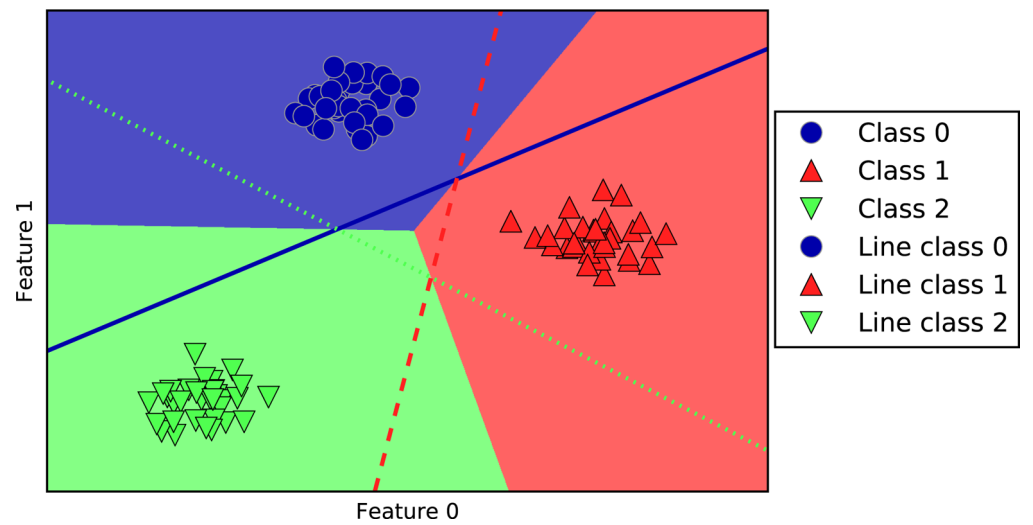
\includegraphics[scale=0.60]{../Imagen_Machine/2D}
	\caption{Límites de decisión aprendidos por los tres clasificadores  one-vs.-rest}
	\label{2D}
\end{figure}



\subsubsection{Fortalezas, debilidades y parámetros}

 El principal parámetro de los modelos lineales es el parámetro de regularización, llamado {\ttfamily alfa}  en los modelos de regresión y $C$ en {\ttfamily LinearSVC} y {\ttfamily LogisticRegression}. Los valores grandes para alfa o pequeños para $C$ significan modelos simples. En particular para los modelos de regresión, ajustar estos es muy importante. Por lo general,  $C$ y {\ttfamily alfa}  se buscan en una escala logarítmica.   La otra decisión que debe tomar es si desea usar la regularización $L1$ o la regularización $L2$. Si asume que solo algunos de características son realmemte importantes, debe usar $L1$. De lo contrario, debe establecer por defecto a $L2$.   $L1$ también puede ser útil si la interpretabilidad del modelo es importante. Como $L1$ solo usará algunas características, es más fácil explicar qué características son importantes para el modelo, y cuáles son los efectos de estas características. 
 

 
Los modelos lineales son muy rápidos de entrenar y también rápidos para predecir. Escalan a conjuntos de datos muy grandes y funcionan bien con datos sparse. Si sus datos consisten en cientos de miles  o millones de muestras, es posible que desee investigar utilizando el solver =  "{}sag"{} opción en {\ttfamily LogisticRegression} y {\ttfamily Ridge}, que puede ser más rápido que el predeterminado en grandes conjuntos de datos.  Otras opciones son las clases {\ttfamily SGDClassifier} y  {\ttfamily SGDRegressor}, que implementa versiones aún más escalables que  los modelos lineales descritos aquí.\\

Otra fortaleza de los modelos lineales es que hacen que ellos son relativamente fácil de entender
cómo  hacen una predicción, mediante las fórmulas que vimos anteriormente para la regresión y la clasificación.  Pero si un conjunto de datos tiene características altamente correlacionadas; en estos casos, los coeficientes pueden ser difíciles de interpretar.\\

Generalmente los modelos lineales funcionan bien cuando el número de características es grande en comparación con el número de muestras.  También se utilizan a menudo en conjuntos de datos muy grandes, simplemente porque no es factible entrenar otros modelos.  Sin embargo, en espacios de menor dimensión, otros modelos podrían producir un mejor rendimiento de generalización. En  la página \pageref{kenrelpag} en la sección  "Máquinas de soporte de vectores kernelized"{},  trataremos algunos ejemplos en los que los modelos lineales fallan.







\vspace{-2cm}	
\hspace{-1cm}
{\fcolorbox{red}{white}{ 		
		\begin{minipage}[16cm]{13.5cm}    %   centrado, largo y ancho                {14cm} 
			\vspace{0.4cm}	
			
			
			\begin{center}
				{\bf{Método de encadenamiento}}
			\end{center}	
			
			
			El método de ajuste de todos los modelos en scikit-learn devuelve en el valor.  Lo que
			permite escribir código como el siguiente, que ya hemos utilizado extensamente en este capítulo:\\
			
			{ \ttfamily   	{\scriptsize{  	 
						
						In[51]:\\		
						{ \color{blue}
							
							\# instantiate model and fit it in one line \vspace{-0.2cm}
							
							logreg = LogisticRegression().fit(X\_train, y\_train) } \\ }}}
			
			
			Aquí, se usa  el valor  retornado del ajuste (del modelo) para luego asignar el modelo entrenado a la variable logreg. Esta concatenación del método (aquí \_\!\!\_init\_\!\!\_  y luego ajusta) se conoce como  método encadenamiento (method chaining). Otra aplicación común del encadenamiento del método en scikit-learn es encajar y predecir en línea:\\
			
			{\ttfamily   	{\scriptsize{  	 
						
						In[52]:\\		
						{ \color{blue}		
							
							logreg = LogisticRegression()  \vspace{-0.2cm}
							
							y\_pred = logreg.fit(X\_train, y\_train).predict(X\_test) } \\}}}
			
			
			
			Por último, incluso se puede hacer la instanciación del modelo, ajuste, y  predicción en línea:\\ 
			
			
			{\ttfamily   	{\scriptsize{  	 
						
						In[53]:\\		
						{ \color{blue}
							
							y\_pred = LogisticRegression().fit(X\_train, y\_train).predict(X\_test) } \\ }}}
			
			
			Aunque esta variante muy corta no es ideal. Están sucediendo muchas cosas en una sola línea, lo que podría dificultar la lectura del código. Además, el modelo ajustado de regresión logística no está almacenado en ninguna variable, por lo que no podemos inspeccionarlo o usarlo para predecir en cualquier otro data.			
		\end{minipage} 
}}\\







\subsection{Clasificadores  Naive   Bayes\index{naive bayes classifiers}} 


Los clasificadores Naive Bayes   (Ingenuos de Bayes) son una familia de clasificadores bastante similares a los  modelos lineales  discutidos en la sección anterior.  Sin embargo, tienden a ser aún más rápidos en el entrenamiento. El precio pagado por esta eficiencia es que los modelos de  naive de Bayes  a menudo proporcionan un rendimiento de generalización que es ligeramente má bajo (malo o peor) que el de los clasificadores lineales como {\ttfamily LinearSVC} y {\ttfamily LogisticRegression}.  La razón de que los modelos naives de Bayes   son tan eficientes se debe a que los parámetros aprenden sobre cada característica individualmente y recopilan las estadísticas simples por clase de cada característica. Hay tres tipos de clasificadores de naives de Bayes  implementados en {\ttfamily  scikit-learn}: 
 GaussianNB, BernoulliNB, y MultinomialNB. 
 
 GaussianNB se puede aplicar a 	cualquier dato continuo, mientras que BernoulliNB asume datos binarios y MultinomialNB asume datos de conteo absoluto (es decir, que cada característica representa un número entero de algo, por ejemlo, con qué frecuencia aparece una palabra en una frase).  BernoulliNB y MultinomialNB se utilizan principalmente en la clasificación de datos de texto. El clasificador BernoulliNB cuenta con qué frecuencia cada característica de cada clase no es cero. Esto se entiende más fácilmente con un ejemplo: \\
 
	
\begin{lstlisting}
In[54]:  X = np.array([[0, 1, 0, 1],         #  dato1
                       [1, 0, 1, 1],         #  dato2
                       [0, 0, 0, 1],         #  dato3
                       [1, 0, 1, 0]])        #  dato4   
         y = np.array([0, 1, 0, 1])
	 
\end{lstlisting}
Aquí, tenemos cuatro puntos de datos, con cuatro características binarias cada uno. Hay dos clases, 0 y 1. Para la clase 0 (el primer y tercer punto de datos), la primera característica es cero dos veces y no cero cero veces, la segunda característica es cero una vez y no cero una vez, y así sucesivamente. Estos mismos recuentos se calculan entonces para los puntos de datos de la segunda clase. Contando las entradas no cero por clase en esencia se ve así:\\

\begin{lstlisting}
In[55]:  counts = {}
         for label in np.unique(y):
             # iterate over each class
             # count (sum) entries of 1 per feature
             counts[label] = X[y == label].sum(axis=0)
         print("Feature counts:\n{}".format(counts))
Out[55]:

    Feature counts:
    {0: array([0, 1, 0, 2]), 1: array([2, 0, 2, 1])}

\end{lstlisting}
		

\noindent Los otros dos modelos naive Bayes, MultinomialNB y GaussianNB, son ligeramente diferentes en el tipos de estadísticas que  calculan.  MultinomialNB tiene en cuenta el valor promedio de cada característica por cada clase, mientras que GaussianNB almacena el valor promedio así como la desviación estándar de cada característica por cada clase.


Para hacer una predicción, se compara un punto de datos con las estadísticas de cada una de las clases,
y se predice la clase con más coincidencia.
 Curiosamente, para MultinomialNB y BernoulliNB, esto conduce a la misma  forma de predicción de los modelos lineales  (véase "Modelos lineales para la clasificación"{} en la página \pageref{Mlineales}).
Desafortunadamente, el {\ttfamily coef\_} para los modelos naives de Bayes   tiene un significado algo diferente que en los modelos lineales, en que {\ttfamily coef\_}  no es lo mismo que $w$.

\subsubsection{Fortalezas, debilidades y parámetros} 

 MultinomialNB y BernoulliNB tienen un único parámetro, {\ttfamily alfa}, que controla la complejidad del modelo. 
 La forma en que {\ttfamily alfa}  funciona consiste en que algoritmo añade a los datos  muchos puntos {\ttfamily alfa} de datos virtuales que tienen valores positivos para todas las características.  Esto resulta en un "suavizado"{}  de las estadísticas. Un {\ttfamily alfa} grande significa mayor suavizado, resultando  modelos menos complejos. El rendimiento del algoritmo es relativamente robusto al ajuste de {\ttfamily alfa}, lo que significa que el ajuste de {\ttfamily alfa} no es crítico para un buen rendimiento.  Sin embargo, por lo general, la afinación mejora un poco la exactitud.\\
 
El GaussianBN se utiliza principalmente en datos con dimensión muy grande, mientras que los otros dos  modelos se utilizan ampliamente para  recuento de datos sparse, como en el caso de  texto. El modelo MultinomialNB generalmente tiene mejores resultados que el  BernoulliNB, particularmente en conjuntos de datos con un número relativamente grande de características distintas de cero (es decir, documentos grandes).\\

Los  modelos naive Bayes   comparten muchas de las fortalezas y debilidades de los modelos lineales. Son muy rápidos para entrenar y predecir, y el procedimiento de entrenamiento es fácil entender. Los modelos funcionan muy bien con datos sparse de alta dimensión y son relativamente robusto a los parámetros. Los modelos naive Bayes  son excelentes modelos de referencia y   a menudo se usan en conjuntos de datos muy grandes, donde la capacitación o el entrenamiento para un modelo lineal puede tardar demasiado.

\subsection{Árboles de decisión\index{árboles de decisión}}

Los árboles de decisión son modelos ampliamente utilizados para tareas de clasificación y regresión. Esencialmente,  aprenden una jerarquía de preguntas if{\scriptsize{/}}else, que lo que lleva a una decisión. \\

Estas preguntas son similares a las que podrías hacer en un juego de 20 preguntas. Imagine que desea distinguir entre los siguientes cuatro animales: osos, halcones, pingüinos y delfines. Su objetivo es llegar a la respuesta correcta haciendo el menor número posible de preguntas. Podría empezar preguntando
 si el animal tiene plumas, una pregunta que reduce el problema a sólo dos  animales.
Si la respuesta es  "{}si"{}, puede hacer otra pregunta que podría ayudarlo a distinguir entre halcones y
pingüinos. Por ejemplo, podría preguntar si el animal puede volar. Si el animal no tiene plumas, sus posibles elecciones de animales son delfines y osos, y  tendrás que hacer una pregunta para distinguir entre estos dos animales, por ejemplo, preguntando si el animal tiene aletas. \\

Esta serie de preguntas puede expresarse como un árbol de decisión, como se muestra en la Figura \ref{Arbol1}.\\

\begin{lstlisting}
In[56]:  mglearn.plots.plot_animal_tree()
\end{lstlisting}

En la Figura \ref{Arbol1} se ilustra el método aplicado al problema de los cuatro animales, cada nodo en el árbol representa una pregunta o un nodo terminal (también llamado hoja) que contiene la respuesta. Los bordes conectan las respuestas a un pregunta con la siguiente pregunta que harías.\\

\begin{figure}[h!]
	\centering
	\includegraphics[scale=0.55]{../Imagen_Machine/Arbol1}
	\caption{Un árbol de decisión para distinguir entre varios animales}
	\label{Arbol1}
\end{figure}



En lenguaje de aprendizaje automático, construimos un modelo para distinguir entre cuatro clases de
animales (halcones, pingüinos, delfines y osos) que usan las tres características "tiene plumas"{}, "puede volar"{}  y  "tiene aletas"{}.   En lugar de construir estos modelos a mano, podemos aprender de ellos a partir de datos mediante el aprendizaje supervisado.


\subsubsection{Construyendo árboles de decisión}


Veamos el proceso de construcción\index{construcción de un árbol} de un árbol de decisión en un conjunto de datos  para una clasificación 2D, que se muestra en la Figura \ref{arbol2D}. El conjunto de datos consta de dos formas de media luna,  cada clase que consta de 75 puntos de datos. Nos referiremos a este conjunto de datos como {\ttfamily two\_moons}.\\

 Un árbol de decisión aprendiendo,  significa aprender la secuencia de preguntas if{\scriptsize/}else que nos lleva a la  respuesta verdadera de forma muy rápida. En el entorno de aprendizaje automático, estas preguntas son llamadas pruebas (que no deben confundirse con el conjunto de pruebas, que son los datos que usamos para probar  qué tan bien generaliza el modelo). Por lo general, los datos no vienen en forma de características binarias sí{\scriptsize/}no  como en el ejemplo animal, en su lugar,  se representa como características continuas como en el conjunto de datos 2D que se muestra en la Figura \ref{arbol2D}. Las pruebas o preguntas que se utilizan en los datos continuos tienen una  forma como:
 
                 "{}¿ Si la característica es mayor que el valor $a$? "{}. \\
 



\begin{figure}[h!]
	\centering
	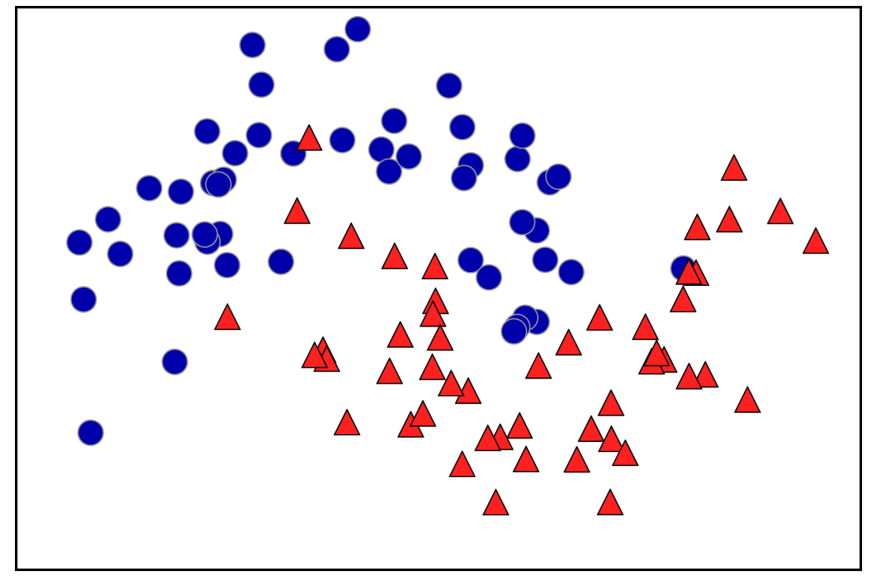
\includegraphics[scale=0.60]{../Imagen_Machine/arbol2D}
	\caption{Conjunto de datos de dos lunas en el que se construirá el árbol de decisión}
	\label{arbol2D}
\end{figure}



Para construir un árbol, el algoritmo busca  todas las pruebas posibles y encuentra la que es
más informativa sobre la variable objetivo. La figura \ref{Arbol3} muestra la primera prueba que es
seleccionada. Dividiendo el conjunto de datos verticalmente en $x[1]=0.0596$  produce la mayor cantidad de información; esta es la mejor separación de los puntos de la clase 1 y de la clase 2.  El nodo superior, también es llamado  Raíz, y representa el conjunto de datos completo,  que en este caso consta de 75 puntos que pertenecen a la clase 0 y 75 puntos pertenecientes a la clase 1. La división se realiza probando si $x[1]<=0.0596$, indicado por una línea negra.  Si la prueba es verdadera, se asigna un punto al nodo izquierdo, que contiene 2  puntos que pertenecen a la clase 0 y 32 puntos que pertenecen a la clase 1.   De lo contrario el punto se asigna al nodo derecho, que contiene  48  puntos que pertenecen a la clase 0 y 18 puntos pertenecientes a la clase 1. Estos dos nodos corresponden a la parte superior y inferior de las regiones que se muestran en la Figura \ref{Arbol3}.  A pesar de que la primera división hizo un buen trabajo de separación clasificando las dos clases, la región inferior todavía contiene puntos que pertenecen a la clase 0, y la región superior todavía contiene puntos que pertenecen a la clase 1.  Podemos construir un  modelo más preciso  repitiendo el proceso de búsqueda de la mejor prueba en ambas regiones. La Figura \ref{Arbol4} muestra que próxima  división más informativa para la región de la izquierda y de la derecha se basa en $x[0]$.



\begin{figure}[h!]
	\centering
	\includegraphics[scale=0.50]{../Imagen_Machine/Arbol3}
	\caption{Límite de decisión del árbol con profundidad 1 (izquierda) y árbol correspondiente (derecha)}
	\label{Arbol3}
\end{figure}


\begin{figure}[h!]
	\centering
	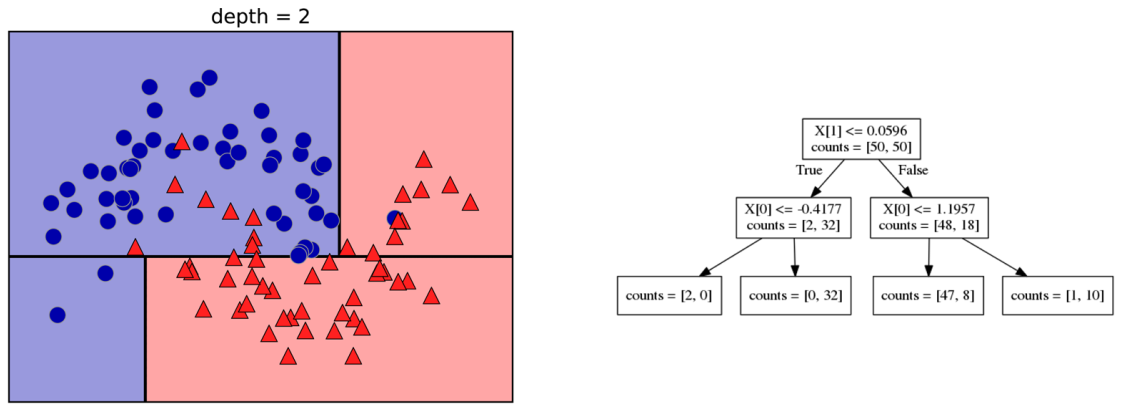
\includegraphics[scale=0.50]{../Imagen_Machine/Arbol4}
	\caption{Límite de decisión del árbol con profundidad 2 (izquierda) y el árbol de decisión correspondiente (derecha)}
	\label{Arbol4}
\end{figure}


Este proceso recursivo produce un árbol binario de decisiones, con cada nodo que contiene una prueba.    Alternativamente, se puede pensar en cada prueba como la división de la parte de los datos que actualmente se está considerando a lo largo de un eje.  Esto produce una visión del algoritmo como la construcción de una partición jerárquica.    Como cada prueba concierne a una sola característica, las regiones de la partición resultante siempre tienen límites de eje paralelo.    La partición recursiva de los datos se repite hasta que cada región de la partición (cada hoja en el árbol de decisiones) sólo contiene un único valor objetivo (una sola clase o un único valor de regresión).    Una hoja del árbol que sólo contiene puntos de datos que comparten el mismo valor objetivo se llama hojas puras. La  partición final de este conjunto de datos se muestra en la Figura \ref{Arbol4}.\\



\begin{figure}[h!]
	\centering
	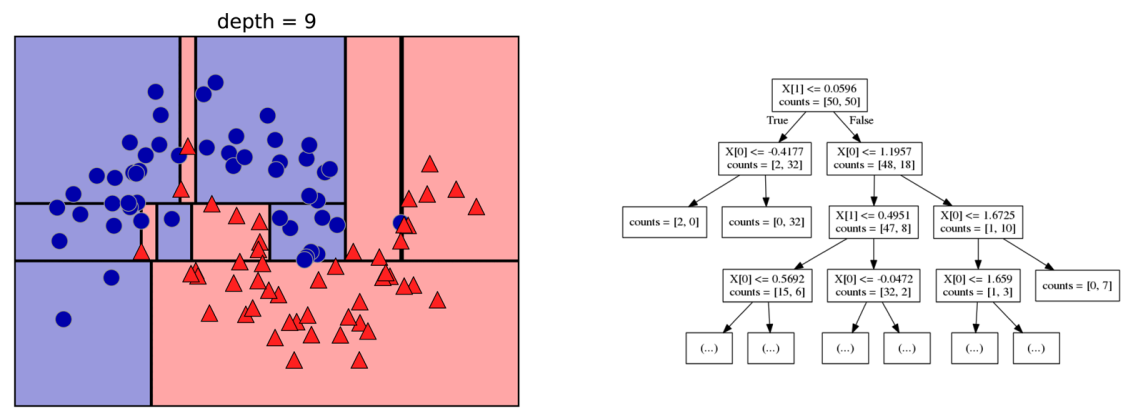
\includegraphics[scale=0.50]{../Imagen_Machine/Arbol5}
	\caption{Límite de decisión del árbol con profundidad 9 (izquierda) y parte del correspondiente
		árbol (derecha); el árbol completo es bastante grande y difícil de visualizar}
	\label{Arbol5}
\end{figure}


Una predicción para un nuevo punto de datos se hace chequeando en qué región de la partición del espacio de la característica se encuentra el punto, y después predice el objetivo por la mayoría (o el objetivo único en el caso de hojas puras) en esa región. La región se puede encontrar atravesando el árbol desde la raíz, yendo a izquierda o derecha, dependiendo de si la prueba se cumple o no. \\

También es posible usar árboles para tareas de regresión, usando exactamente la misma técnica. Para hacer una predicción, atravesamos el árbol basado en las pruebas en cada nodo y encontramos la hoja en la que cae el nuevo punto de datos. El resultado para este punto de datos es el objetivo medio de los puntos de entrenamiento en esta hoja.


\subsubsection{Controlar la complejidad de los árboles de decisión.}

Típicamente, construir un árbol como se describe aquí y continuar hasta que todas las hojas sean puras
conduce a modelos que son muy complejos y altamente ajustados a los datos de entrenamiento.  La presencia de hojas puras significa que el árbol es 100\% exacto en el conjunto de entrenamiento; cada punto de datos en el conjunto de entrenamiento está en una hoja que tiene la clase de mayoría correcta.  El sobreajuste se puede ver a la izquierda de la Figura \ref{Arbol5}. Donde se se observan las regiones determinadas para la clase 1 en medio de todos que pertenecen a la clase 0. Por otro lado, hay una pequeña franja predicha como clase 0 alrededor del punto que pertenece a la clase 1 a muy a la derecha. Esta no es la forma en que uno podría imaginar el límite de decisión para observar, y el límite de decisión se centra mucho en los puntos atípicos únicos que están lejos de los otros puntos de esa clase.\\



Hay dos estrategias comunes para evitar el sobreajuste: detener la creación del árbol temprano (también llamado pre-poda o poda previa, del inglés pre-pruning), o construir el árbol y luego  remover los nodos que contienen poca información (también llamado  poda posterior  o simplemente poda, del inglés post-poda). Los criterios posibles para la pre-poda   incluyen limitar la profundidad máxima del árbol, limitar el número máximo de hojas, o requerir un número mínimo de puntos en un nodo para seguir dividiéndolo. 

 En {\ttfamily scikit-learn} los árboles de decisión se implementan para regresión con {\ttfamily DecisionTreeRegressor}, y con {\ttfamily DecisionTreeClassifier} para clasificar; además, scikit-learn solo implementa la  pre-poda, y no post-poda. \\


El efecto de la pre-poda lo podemos ver con más detalle en el conjunto de datos de Cáncer de Mama (Breast Cancer).  La metodología se implementa como siempre, primero importamos el conjunto de datos y lo dividimos en entrenamiento y prueba, y luego se construye el modelo. Si se usa la  configuración por defecto, se  desarrolla completamente el árbol (el árbol crece  hasta que todas las hojas son puras). Y fijamos el {\ttfamily random\_state} en el árbol, que se usa para desempate internamente:\\


\begin{lstlisting}
In[58]:  from sklearn.tree import DecisionTreeClassifier
      
         cancer = load_breast_cancer()
         X_train, X_test, y_train, y_test = train_test_split(cancer.data,
              cancer.target, stratify=cancer.target, random_state=42)
         tree = DecisionTreeClassifier(random_state=0)
         tree.fit(X_train, y_train)
         print("Accuracy on training set: {:.3f}".format(tree.score(
                X_train, y_train)))
         print("Accuracy on test set: {:.3f}".format(tree.score(
                X_test, y_test)))

Out[58]:

      Accuracy on training set: 1.000
      Accuracy on test set: 0.937

\end{lstlisting}


Como era de esperar, la exactitud en el conjunto de entrenamiento es del 100\%, porque las hojas son puras, el árbol creció lo suficientemente profundo como para poder memorizar perfectamente todas las etiquetas en los datos de entrenamiento. La exactitud del conjunto de prueba es ligeramente menor a la del conjoto de entrenamiento, o mala y aun peor que en los modelos lineales que vimos anteriormente, que tenían alrededor de 95\% de exactitud.\\


Si no restringimos la profundidad de un árbol de decisión, el árbol puede volverse arbitrariamente profundo
y complejo. Por lo tanto, los árboles no podados son propensos al sobreajuste y en consecuencia no generalizan
bien (sobre nuevos datos).  Ahora apliquemos la poda previa al árbol, que limita el desarrollo
del árbol antes de alcanzar un ajuste perfecto con los datos de entrenamiento.  Una opción es dejar de construir el árbol después de que se haya alcanzado cierta profundidad. En este caso establecemos {\ttfamily max\_depth} = 4, que significa solo se pueden hacer cuatro preguntas consecutivas (ver Figuras \ref{Arbol3} y \ref{Arbol5}). Limitando la profundidad del árbol disminuye el sobreajuste, lo cual debe conducir a una menor exactitud en el conjunto de entrenamiento:\\


\begin{lstlisting}
In[59]:  tree = DecisionTreeClassifier(max_depth=4, random_state=0)
         tree.fit(X_train, y_train)
         print("Accuracy on training set: {:.3f}".format(tree.score(
                X_train, y_train)))
         print("Accuracy on test set: {:.3f}".format(tree.score(
                X_test, y_test)))

Out[59]:

    Accuracy on training set: 0.988
    Accuracy on test set: 0.951
\end{lstlisting}


\subsubsection{Analizando árboles de decisión}

Podemos visualizar el árbol empleado  la función {\ttfamily{export\_graphviz}} del módulo {\ttfamily .tree}  (árbol). Esta función  escribe un archivo  de texto en formato  .dot. Establecemos una opción para colorear los nodos a fin  reflejar la clase mayoritaria en cada nodo, y se dan los nombres de clase y características para que el árbol pueda etiquetarse correctamente:\\


\begin{lstlisting}
In[60]:  from sklearn.tree import export_graphviz
         export_graphviz(tree, out_file="tree.dot", 
                         class_names=["malignant", "benign"],
                         feature_names=cancer.feature_names, 
                         impurity=False, filled=True)

\end{lstlisting}

Podemos leer este archivo y visualizarlo, como se ve en la Figura \ref{ArbolCacer}, usando el modulo {\ttfamily graphviz} o  usar cualquier programa que pueda leer archivos .dot:\\

\begin{lstlisting}
In[61]:  import graphviz
         
         with open("tree.dot") as f:
             dot_graph = f.read()
         graphviz.Source(dot_graph)

\end{lstlisting}



\begin{figure}[h!]
	\centering
	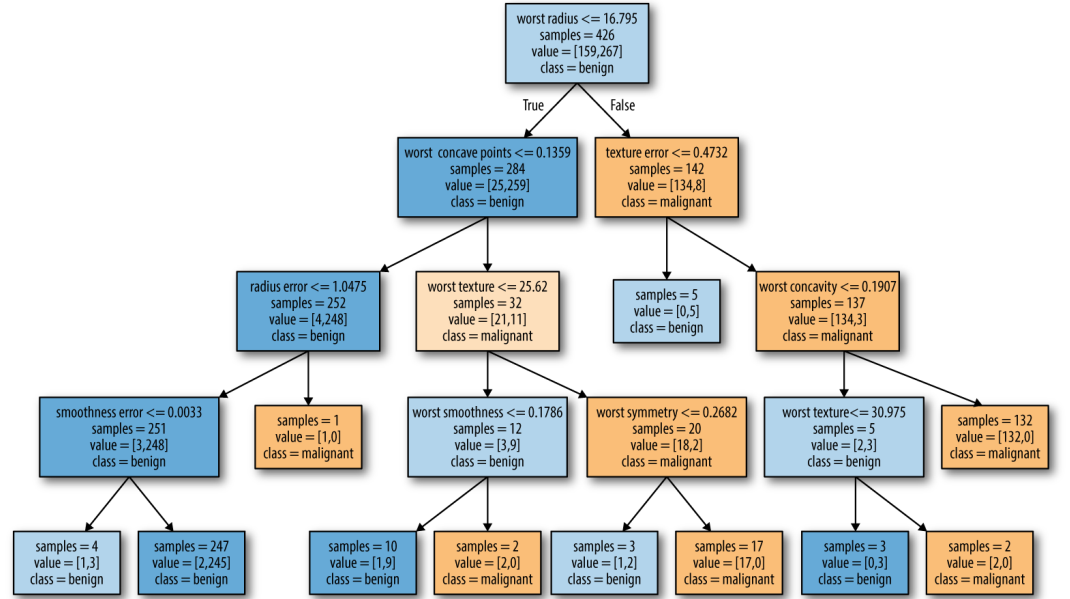
\includegraphics[scale=0.50]{../Imagen_Machine/ArbolCacer}
	\caption{Límite de decisión del árbol con profundidad 9 (izquierda) y parte del correspondiente
		árbol (derecha); el árbol completo es bastante grande y difícil de visualizar}
	\label{ArbolCacer}
\end{figure}



La visualización del árbol proporciona una idea muy clara de cómo el algoritmo
hace predicciones y es un buen ejemplo de un algoritmo de aprendizaje automático que puede ser 
explicado fácilmente a los inexpertos.  Sin embargo, incluso con un árbol de profundidad, como se ve aquí,  el árbol puede volverse un poco abrumador. Árboles más profundos (una profundidad de 10 es poco común, pero puede ser) son aún más difíciles de comprender.

Un método  útil  para inspeccionar el árbol  con la finalidad  de averiguar qué ruta toma la mayoría de los datos, son las  {\ttfamily n\_samples}  (n\_muestras) que se muestran en cada nodo, como en la Figura \ref{ArbolCacer}  donde se ve claramente el  número de muestras en cada nodo, mientras que el valor da el número de muestras por clase. Siguiendo las ramas a la derecha, vemos que  worst radius $<=16.795$ (peor radio)  crea un nodo que contiene  8 benignos y 134  malignas.  El resto de este lado del árbol utiliza algunas distinciones más finas para dividir estas 8 muestras benignas restantes.   De las 142 muestras que quedaron  a la derecha en la división inicial, casi todos (132) terminan en la hoja de la derecha.\\

Tomando  a la izquierda en la raíz, para el worst radius $> 16.795$ (peor radio) terminamos con 25 malignos
y 259 muestras benignas. Casi todas las muestras benignas terminan en la segunda hoja, 
a la derecha, la mayoría de las otras hojas  contienen muy pocas muestras.\\


\subsubsection{Importancia de la característica en árboles} \label{ImpotCaract}

 En lugar de observar todo el árbol  que puede ser  agobiante,  podemos usar algunos propiedades 
 derivadas del resumen  de la ejecusión del árbol. El  resumen más común  utilizado es la importancia de la característica, que califica la importancia de cada característica por la decisión que toma un árbol.  Este es un número entre 0 y 1 para cada característica, donde 0 significa  "{}no utilizado en absoluto"{},  y 1 significa  "{}predice perfectamente el objetivo"{}, y la sumatoria  total de las importancias  de las características  es igual a 1:\\
  
\begin{lstlisting}
In[62]:  print("Feature importances:\n{}".format(tree.feature_importances_))

Out[62]:

    Feature importances:
    [ 0.     0.   0.     0.     0.     0.     0.     0.    0.   0.     0.01
      0.048  0.   0.     0.002  0.     0.     0.     0.    0.   0.727  0.046
      0.     0.   0.014  0.     0.018  0.122  0.012  0. ]
\end{lstlisting}


Podemos visualizar las importancias de las características de una manera similar a la forma en que visualizamos los coeficientes en el modelo lineal (Figure \ref{ImpotanciaCaract}):



\begin{lstlisting}
  
In[63]:  def plot_feature_importances_cancer(model):
             n_features = cancer.data.shape[1]
             plt.barh(range(n_features), model.feature_importances_, 
                      align='center')
             plt.yticks(np.arange(n_features), cancer.feature_names)
             plt.xlabel("Feature importance")
             plt.ylabel("Feature")
             plot_feature_importances_cancer(tree)
\end{lstlisting}



\begin{figure}[h!]
	\centering
	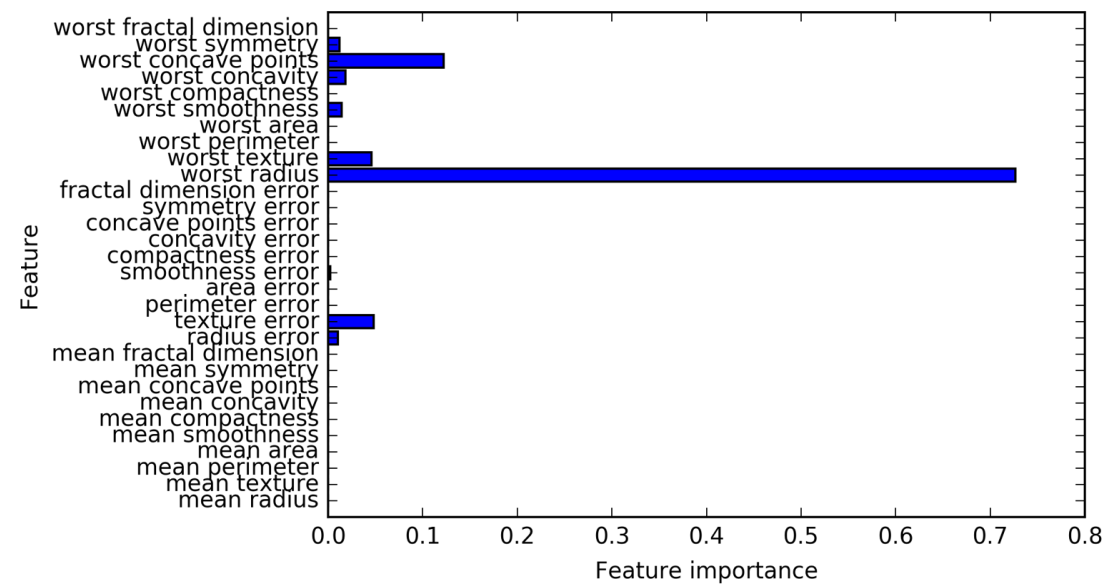
\includegraphics[scale=0.50]{../Imagen_Machine/ImpotanciaCaract}
	\caption{Importancia de características calculadas a partir de un árbol de decisión aprendido en el  conjunto de datos de Cáncer de Mama}
	\label{ImpotanciaCaract}
\end{figure}


Aquí vemos que la característica utilizada en la división superior es "{}worst radius"{}  (peor radio),  y resulta ser  la característica más importante. Esto confirma nuestra observación al analizar el árbol que en el primer nivel ya separa  bastante bien las dos clases. 

Sin embargo, si una característica aparece con  un puntaje  bajo  de importancia  en  {\ttfamily{ feature\_importance}},  no significa que esta característica no aporte información, sólo significa que la característica no fue seleccionada por el árbol, probablemente porque otra característica codifica la misma información.\\


En contraste con los coeficientes de los modelos lineales, la  importancia de características en este caso son siempre positivas, y no codifican de qué clase es indicativa una característica. El valor de  importancia de la  característica nos dicen que el "{}worst radius"{ }  es importante; pero no dice, si un radio alto es indicativo de una muestra que es benigna o maligna. De hecho, puede que no haya una relación tan simple entre características y clase, como se puede ver en el siguiente ejemplo (Figuras \ref{EtiquetArbol1}  y \ref{EtiquetArbol1} ):\\

 

\begin{lstlisting}
In[64]:  tree = mglearn.plots.plot_tree_not_monotone()
         display(tree)
Out[64]:

    Feature importances: [ 0. 1.]

\end{lstlisting}


\begin{figure}[h!]
	\centering
	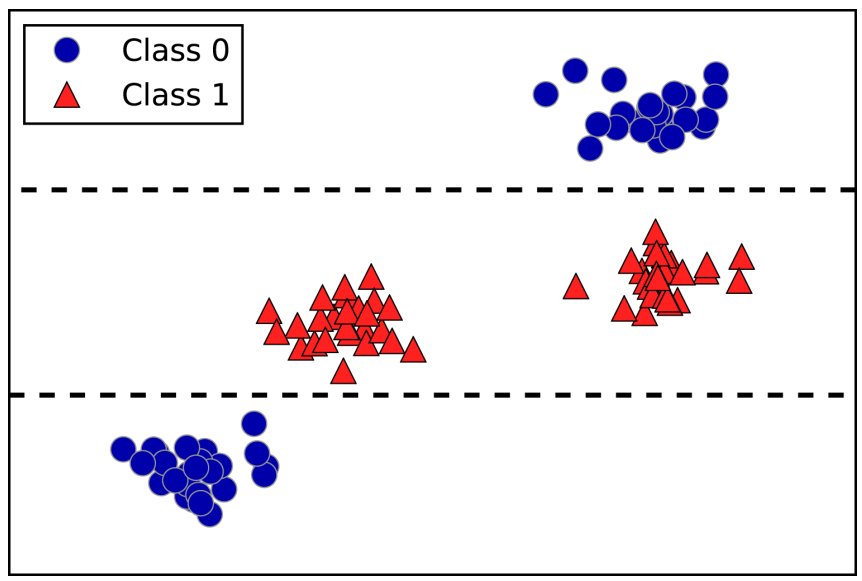
\includegraphics[scale=0.45]{../Imagen_Machine/EtiquetArbol1}
	\caption{Conjunto de datos bidimensionales en el que la característica en el eje y tiene una relación no monótona con la etiqueta de clase, y los límites de decisión encontrados por un árbol de decisiones}
	\label{EtiquetArbol1}
\end{figure}



\begin{figure}[h!]
	\centering
	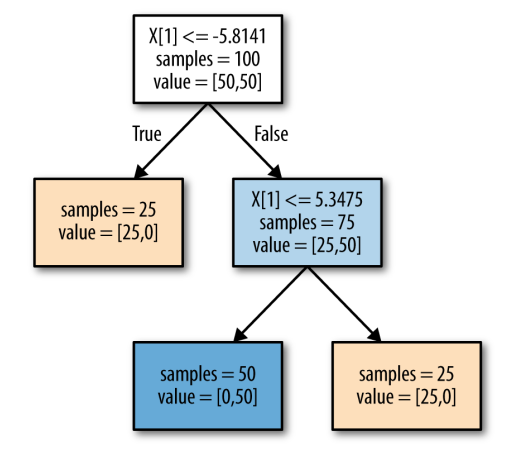
\includegraphics[scale=0.50]{../Imagen_Machine/EtiquetArbol2}
	\caption{Árbol de decisión aprendido en los datos mostrados en la Figura \ref{EtiquetArbol1}}
	\label{EtiquetArbol2}
\end{figure}



El gráfico \ref{EtiquetArbol1} muestra un conjunto de datos con dos características y dos clases. En este caso  toda la información está contenido en $X[1]$, y $X[0]$ no se utiliza en absoluto. Pero la relación entre $X[1]$ y la clase de salida no es monótona, lo que significa que no podemos decir que "{}un valor alto de $X[0]$ significa clase 0, y un valor bajo significa clase 1{}  o viceversa.\\

Mientras centramos nuestra discusión aquí en los árboles de decisión para la clasificación, todo lo dicho  es igualmente válido en árboles de decisión para la regresión, que se implementa en la
 {\ttfamily{DecisionTreeRegressor}}.  El uso y análisis de los árboles de regresión es muy similar al de
Árboles de clasificación. Sin embargo, hay una propiedad particular e  importante de tener presente al usar modelos basados en árboles para la regresión, se trata de que el  {\ttfamily{DecisionTreeRegressor}} (y todos los otros modelos de regresión basados en árboles) no es capaz de extrapolar, o hacer predicciones fuera del rango de los datos de entrenamiento.\\


Veamos  esto con más detalle, utilizando un conjunto de datos de los precios históricos de las memorias  para un ordenador (RAM). La Figura \ref{RAM} muestra el conjunto de datos, con la fecha en el eje $x$ y el precio de un megabyte de RAM en ese año en el eje $y$:\\


\begin{lstlisting}
In[65]:  import pandas as pd
         ram_prices = pd.read_csv("data/ram_price.csv")
         
         plt.semilogy(ram_prices.date, ram_prices.price)
         plt.xlabel("Year")
         plt.ylabel("Price in $/Mbyte")
\end{lstlisting}



\begin{figure}[h!]
	\centering
	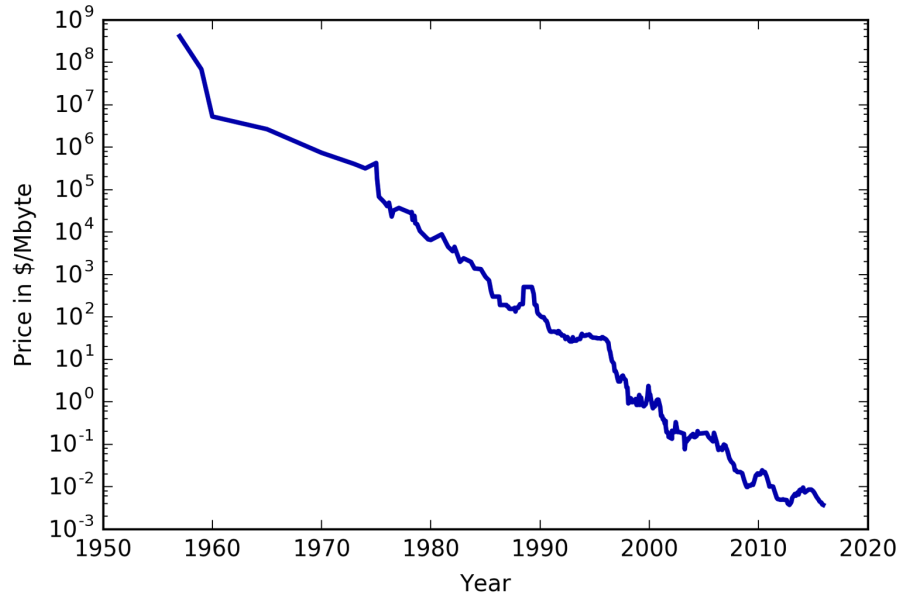
\includegraphics[scale=0.50]{../Imagen_Machine/RAM}
	\caption{Evolución histórica del precio de la RAM, trazada en una escala logarítmica}
	\label{RAM}
\end{figure}


Se plantea  un pronóstico para los años posteriores a 2000, utilizando los datos históricos hasta ese 
punto, con la fecha como única  característica en el eje $x$.  Al re-escalar los precios, en este caso  $y$, mediante el logarítmo, la relación se hace relativamente lineal con algunas pequeñas variaciones,   y por lo tanto  será más fácil de predecir con los modelos lineales. Se costruyen y se comparan los modelos sobre la misma gráfica: mediante {\ttfamily DecisionTreeRegressor} y {\ttfamily LinearRegression}.  Después de entrenar  los modelos,  se hacen las predicciones sobre el conjunto  de prueba y se evalúa:\\


%   Esto no hace una diferencia para {\ttfamily DecisionTreeRegressor}, pero hace una gran diferencia para   {\ttfamily LinearRegression} ( discutiremos esto con más profundidad en el Capítulo \ref{Cap4}). 

\begin{lstlisting}
In[66]:  from sklearn.tree import DecisionTreeRegressor
         # use historical data to forecast prices after the year 2000
         data_train = ram_prices[ram_prices.date < 2000]
         data_test = ram_prices[ram_prices.date >= 2000]
         
         # predict prices based on date
         X_train = data_train.date[:, np.newaxis]
         # we use a log-transform to get a simpler relationship of data to target
         y_train = np.log(data_train.price)
         
         tree = DecisionTreeRegressor().fit(X_train, y_train)
         linear_reg = LinearRegression().fit(X_train, y_train)
         
         # predict on all data
         X_all = ram_prices.date[:, np.newaxis]
         
         pred_tree = tree.predict(X_all)
         pred_lr = linear_reg.predict(X_all)
         
         # undo log-transform
         price_tree = np.exp(pred_tree)
         price_lr = np.exp(pred_lr)
\end{lstlisting}



\begin{figure}[h!]
	\centering
	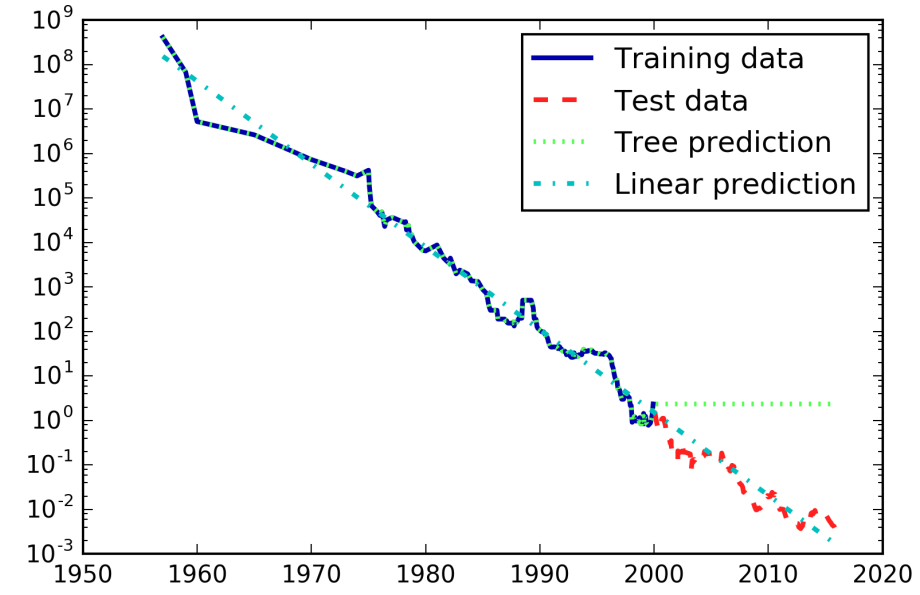
\includegraphics[scale=0.50]{../Imagen_Machine/RAM2}
	\caption{Comparación de predicciones hechas por un modelo lineal y las predicciones hechas
		por un árbol de regresión sobre los datos de precios de la memoria RAM}
	\label{RAM2}
\end{figure}


\begin{lstlisting}
In[67]:  plt.semilogy(data_train.date, data_train.price, 
                       label="Training data")
         plt.semilogy(data_test.date, data_test.price, label="Test data")
         plt.semilogy(ram_prices.date, price_tree, label="Tree prediction")
         plt.semilogy(ram_prices.date, price_lr, label="Linear prediction")
         plt.legend()
\end{lstlisting}


La diferencia entre los modelos es bastante sorprendente. El modelo lineal se aproxima a
los datos con una línea, como lo esperado.  Esta línea proporciona un pronóstico bastante bueno para los datos de prueba (los años posteriores a 2000), mientras pasa por alto algunas de las variaciones más finas en tanto el entrenamiento como los datos de prueba.  Por otro lado,  el modelo de árbol hace perfecto predicciones sobre los datos de entrenamiento; claro, no restringimos la complejidad del árbol, por lo que aprendió todo el conjunto de datos.  Sin embargo, una vez que dejamos el rango de la data entrenamiento, el modelo simplemente sigue prediciendo por el último punto conocido.  El árbol no tiene la capacidad para generar  "{}nuevas"{}  respuestas, fuera de lo que memorizó o aprendió en la data de entrenamiento. Esta deficiencia se presenta  en todos los modelos basados en árboles. \\

\subsubsection{Fortalezas, debilidades y parámetros}


Como se discutió anteriormente, los parámetros que controlan la complejidad del modelo de árboles de decisión son los parámetros como el de pre-poda,  que detienen la construcción del árbol antes de que esté completamente desarrollado. Por lo general, elegir una de las estrategias que controlan la complejidad del modelo (como {\ttfamily max\_depth,  max\_leaf\_nodes}  o {\ttfamily min\_samples\_leaf}): es suficiente para evitar el sobreajuste.\\

Los árboles de decisión tienen dos ventajas sobre muchos de los algoritmos que hemos discutido:
Primero el modelo resultante puede ser fácilmente visualizado y comprendido por inexpertos (al menos en árboles más pequeños).  Segundo los algoritmos son completamente invariate  a la escala de la data.  Como cada característica es procesada por separado,  las  divisiones posibles de la data no dependerá de la escala, no es necesario ningún proceso previo como la normalización o estandarización de características para los algoritmos del árbol de decisiones.   En particular, los árboles de decisión funcionan bien cuando
tiene características que están en escalas completamente diferentes, o una combinación de binario y continuas.\\


El principal inconveniente de los árboles de decisión es que incluso con el uso de la pre-poda,
tienden a sobreajustar y en consecuencia proporciona un rendimiento de generalización deficiente.  Por lo tanto, para eludir este problema se plantean los  métodos de conjuntos de áboles (Ensembles of Decision Trees). Generalmente en la mayoría aplicaciones  se usa estos  métodos,  en lugar de un simple  árbol de decisión. \\

A continuación se tratan algunos de los métodos de conjuntos de áboles. 


\subsection{Conjuntos de árboles de decisión \\
	(Ensembles of Decision Trees)}


Los métodos de conjunto  son técnicas  que combinan múltiples modelos de aprendizaje automático para crear modelos más potentes. Existen muchos modelos en la literatura de aprendizaje automático que pertenecen a esta categoría, pero hay dos modelos de conjunto que han demostrado ser eficaz en una amplia gama de conjuntos de datos para clasificación y regresión,  ambos usan árboles de decisión en sus bloques de construcción: bosques aleatorios (random forests) y  árboles de decisión potenciado  
o simplemente potenciación del gradiente (gradient boosted decision trees).  

\subsubsection{Bosques Aleatorios}


El pricipal inconveniente  de los árboles de decisión, es que tienden a generar sobreajuste en la  data de entrenamiento. Un forma de abordar este problema es con  bosques aleatorios\index{bosques aleatorios}. Esencialmente un bosque aleatorio es  una colección de árboles de decisión, donde cada árbol es ligeramente diferente de los demás. La idea de fondo de los bosques aleatorios es reducir el sobreajuste en los modelos de árbol de decisión, pues cada árbol seguro hace un buen trabajo de predicción, pero probablemente  sobreajustará  gran parte de los datos. Si construimos muchos  árboles, todos los cuales funcionan bien y se sobreajustan de diferentes maneras, podemos reducir la cantidad  del sobreajuste promediando sus resultados. Esta reducción en el sobreajuste, mientras se conserva  el poder predictivo de los árboles puede ser  demostrado usando matemáticas rigurosas (para mayor información revisar The Elements of Statistical Learning (Springer) by Trevor Hastie, Robert Tibshirani, and Jerome Friedman). \\

Para implementar esta estrategia, necesitamos construir muchos árboles de decisión.  Cada árbol debe hacer un trabajo aceptable de predicción del objetivo, y también debe ser diferente de los otros arboles. Los bosques aleatorios obtienen su nombre al incorporar la aleatoriedad en la construcción del árbol.
 
Para garantizar la diferencia entre los árboles, hay dos formas de construir los árboles que formarán los bosques: una consiste en  seleccionar diferentes conjuntos de puntos de datos para usarlos en la construción del árbol, y la otra forma es emplear una  selección aleatoria ponderada de  las características en cada nodo a dividir.  En la próxima sección se analiza  este proceso con más detalle.\\


\subsubsection{Construyendo Bosques  Aleatorios}


Para construir un modelo de bosque aleatorio, necesitamos decidir sobre el número de árboles a emplear. Esta acción se define en el parámetro {\ttfamily n\_estimators} de {\ttfamily RandomForestRegressor} o {\ttfamily RandomForestClassifier}.   Por ejemplo, decidimos  construir un bosques con 10 árboles, estos árboles serán construido completamente independiente  uno del otro, y el algoritmo hará  diferentes selecciones aleatorias  para cada árbol, asegurado que los árboles sean distintos.   
Para construir un árbol, primero tomamos lo que se llama una muestra de Bootstrap (muestra de arranque) en la data. El proceso consiste en extraer n\_muestras con reemplazo de la data (n\_muestras puntos de datos), es decir,  el conjunto creado que es tan grande como el conjunto de datos original, pero algunos puntos de datos se repetirán varias veces, y otros faltarán, aproximadamente un tercio. \\

Para ilustrar esta situación, supongamos que queremos crear un bootstrap de la lista ["{}a"{} , "{}b"{}, "{}c"{}, "{}d"{}].
 Una posible muestra de bootstrap sería ["{}b"{}, "{}d"{}, "{}d"{}, "{}c"{}]. Otro posible muestra sería ["{}d"{}, "{}a"{}, "{}d"{}, "{}c"{} ].\\



El paso siguiente es costruir un árbol de decisión basado en este conjunto de datos recién creado. Sin embargo, el algoritmo que describimos para el árbol de decisión está ligeramente modificado. En lugar de buscar la mejor prueba para cada nodo, en cada nodo el algoritmo selecciona aleatoriamente un subconjunto de las características, y busca la mejor prueba posible que involucre una de estas características. El número de características a seleccionar es controlado por el parámetro {\ttfamily max\_features}. Esta selección de un subconjunto de características se repite por separado en cada nodo, de modo que cada  nodo en un árbol puede tomar una decisión utilizando un subconjunto diferente de las características.\\


El bootstrap  permite que  cada árbol de decisión, en el bosque aleatorio empiece su construcción 
sobre un conjunto de datos ligeramente diferente.  Debido a la elección aleatoria de características en cada nodo, la dividisión  en cada árbol opera con un subconjunto diferente de características. Estos dos mecanismos juntos aseguran que todos los árboles en el bosque aleatorio sean diferentes.\\



Un parámetro crítico en este proceso es {\ttfamily{ max\_features}}. Observe, si se configura {\ttfamily max\_features}  para   {\ttfamily{n\_features}},  significa que cada división puede ver todas las características del conjunto de datos y no ejecutará la aleatoriedad en la selección de características (sin embargo, la aleatoriedad debida al bootstrap permanece).  Si configuramos {\ttfamily max\_features} igual a  1, significa que las divisiones no tienen ninguna opción en absoluto sobre qué característica probar, y sólo pueden buscar sobre diferentes umbrales para la característica que fué seleccionada  al azar. Por lo tanto, un alto {\ttfamily{max\_features}} significa que los árboles en el bosque aleatorio serán bastante similares, y serán capaz de ajustar los datos fácilmente, utilizando las características más distintivas. Un valor bajo para  {\ttfamily{max\_features}},  significa que los árboles en el bosque aleatorio serán bastante diferentes, y que cada árbol podria necesitar ser muy profundo para ajustarse bien a los datos.\\
 
 
Para hacer una predicción usando el bosque aleatorio, el algoritmo primero hace una predicción
por cada árbol en el bosque.  Para la  regresión,  promedia  estos resultados para obtener nuestro predicción final.  Y en el caso de la clasificación, se utiliza una estrategia de "{}votación suave"{} ( "{}soft voting"{}). Esto significa que cada algoritmo hace una predicción "{}suave"{}, proporcionando una probabilidad para cada etiqueta de salida posible. Se promedian las probabilidades predichas por todos los árboles y la clase con la mayor probabilidad  se predice.

\subsubsection{Analizando bosques Aleatorio} 

Para analizar esta técnica, construimos un bosque aleatorio con cinco árboles de decisión sobre la data  {\ttfamily two\_moons}:\\



\begin{lstlisting}
In[68]: from sklearn.ensemble import RandomForestClassifier
	from sklearn.datasets import make_moons
	
	X, y = make_moons(n_samples=100, noise=0.25, random_state=3)
	X_train, X_test, y_train, y_test = train_test_split(X, y, 
	       stratify=y, random_state=42)
	       
	forest = RandomForestClassifier(n_estimators=5, random_state=2)
	forest.fit(X_train, y_train)
\end{lstlisting}

Los árboles que se construyen como parte del bosque aleatorio se almacenan en el atributo {\ttfamily{estimador\_}}.  Los límites de decisión aprendidos por cada árbol, junto con su predicción  generada por el bosque se visualiza en la Figura \ref{Prome5Arbol}:\\


\begin{lstlisting}
In[69]: fig, axes = plt.subplots(2, 3, figsize=(20, 10))
	for i, (ax, tree) in enumerate(zip(axes.ravel(), 
	                                   forest.estimators_)):
        ax.set_title("Tree {}".format(i))
        mglearn.plots.plot_tree_partition(X_train,
    	                                  y_train, tree, ax=ax)
    	
	mglearn.plots.plot_2d_separator(forest, X_train,fill=True,
	                                ax=axes[-1, -1], alpha=.4)
	                                
	axes[-1, -1].set_title("Random Forest")
	mglearn.discrete_scatter(X_train[:, 0], X_train[:, 1], y_train)
\end{lstlisting}



	\begin{figure}[h!]
	\centering
	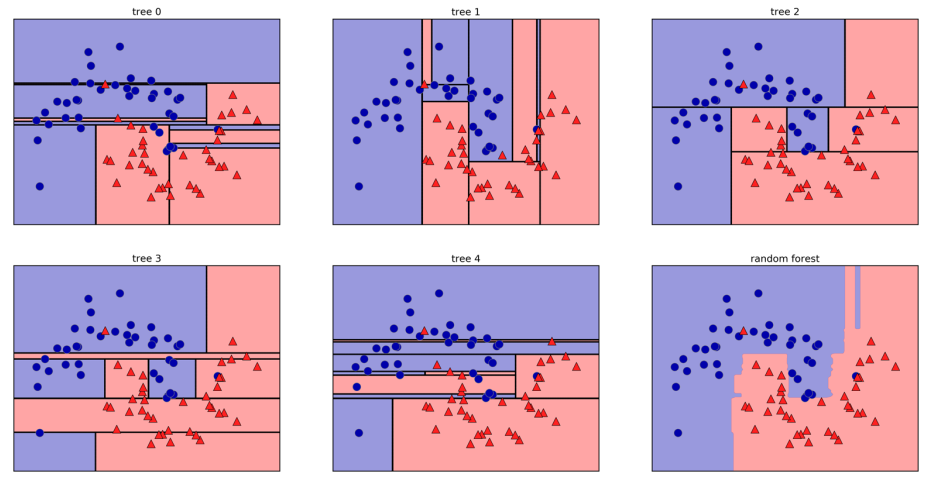
\includegraphics[scale=0.60]{../Imagen_Machine/Prome5Arbol}
	\caption{Límites de decisión encontrados por cinco árboles de decisión aleatorios y el  límite decisión obtenido promediando sus probabilidades predichas}
	\label{Prome5Arbol}
\end{figure}



Se puede ver claramente, que los límites de decisión aprendidos por los cinco árboles son bastante diferentes. Cada uno de ellos comete algunos errores, ya que algunos de los puntos de entrenamiento que se trazan aquí, no se incluyeron en los conjuntos de entrenamiento de los árboles, debido a la muestra de bootstrap.\\

El bosque aleatorio se sobreajusta menos que cualquiera de los árboles individuales, y proporciona un
límite de decisión mucho más intuitivo. En cualquier aplicación real, usaríamos muchos
más árboles (a menudo cientos o miles), lo que lleva a límites aún más suaves.\\

 

			


Como otro ejemplo, apliquemos un bosque aleatorio que consta de 100 árboles sobre la data Cáncer de Mama (Breast Cancer):\\

\begin{lstlisting}
In[70]: X_train, X_test, y_train, y_test = train_test_split(
	     cancer.data, cancer.target, random_state=0)
	forest = RandomForestClassifier(n_estimators=100, random_state=0)
	forest.fit(X_train, y_train)
	
	print("Accuracy on training set: {:.3f}".format(forest.score(X_train, y_train)))
	print("Accuracy on test set: {:.3f}".format(forest.score(X_test, y_test)))

Out[70]:

	Accuracy on training set: 1.000
	Accuracy on test set: 0.972

\end{lstlisting}



El bosque aleatorio nos da una exactitud del 97\%, mejor que los modelos lineales o un único árbol de decisión, sin ajustar ningún parámetro. Podríamos configurar el {\ttfamily max\_features}, o aplicar la  pre-poda como se hizo  para el árbol de decisión simple. Sin embargo, a menudo los parámetros por defecto en el bosque aleatorio ya funcionan bastante bien. De manera similar al árbol de decisión, el bosque aleatorio proporciona las características más importantes, que se calculan agregando  a los bosques la sentencia {\ttfamily feature\_importances\_}. Típicamente, las características de importancia proporcionadas por el bosque aleatorio son más confiables que las proporcionados por un sólo árbol. Observe la figura \ref{ImporTanciBosque}.


\begin{lstlisting}  % [frame=single]	

In[71]: plot_feature_importances_cancer(forest)

\end{lstlisting}



\begin{figure}[h!]
	\centering
	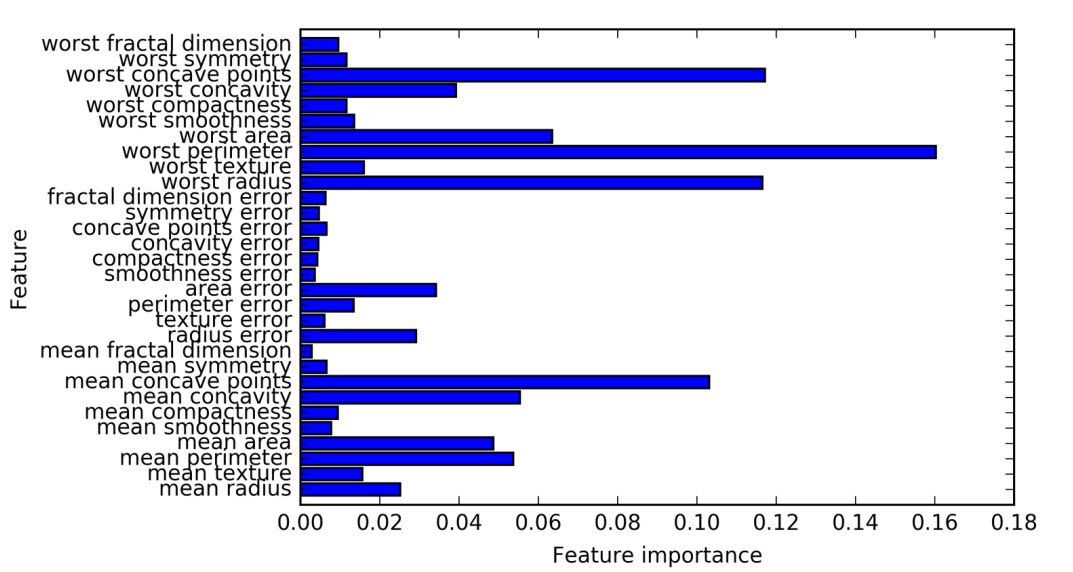
\includegraphics[scale=0.50]{../Imagen_Machine/ImporTanciBosque}
	\caption{Importancia de características calculadas a partir del bosque aleatorio sobre la data de cáncer de mama}
	\label{ImporTanciBosque}
\end{figure}

Como puede ver, el bosque aleatorio le da una importancia distinta de cero a  más características,
que un solo árbol. De manera similar al árbol de decisión simple, el bosque aleatorio también da
gran importancia a la característica de “worst radius”, pero en  elige  “worst perimeter”  ({}"peor perímetro"{})  como  la característica más informativa.



 La aleatoriedad en la construcción de los bosques aleatorios obliga al algoritmo a considerar más explicaciones posibles, el resultado es que el bosque aleatorio captura  mucho más información  de los datos, que un solo árbol.




\subsubsection{Fortalezas, debilidades y parámetros}

 Bosques aleatorios para regresión y clasificación estan actualmente entre los métodos de aprendizaje automático más utilizados. Son muy potentes, y a menudo funcionan bien sin grandes ajuste de los parámetros, y no requieren escalar la data.  \\
 
 
 
 
 Esencialmente, los bosques aleatorios comparten todos los beneficios de los árboles de decisión, al tiempo que compensan algunas de sus deficiencias.  Una razón para  utilizar árboles de decisión es cuando se necesita una representación compacta del proceso de toma de decisiones.  Básicamente es imposible interpretar decenas o cientos de árboles en detalle, y los árboles en bosques aleatorios tienden a ser más profundo que los árboles de decisión (debido al uso de subconjuntos de características).  Por lo tanto si necesita resumir la predicción haciendola de una manera visual a los inexpertos, un árbol de decisión simple podría ser una buena opción.   Al construir bosques aleatorios para data grandes podría consumir algún  tiempo significante; sin embargo, puede ser tratado en paralelo a través de múltiples núcleos del CPU dentro de un ordenador fácilmente;  si está utilizando un procesador multi-core (como casi todos los ordenadores modernos lo hacen), puede utilizar el parámetro {\ttfamily n\_jobs} para ajustar el número de núcleos a utilizar. Usando más núcleos de CPU resultará en velocidad lineal (usando dos núcleos, el entrenamiento del bosque aleatorio será el doble de rápido), pero especificando {\ttfamily n\_jobs} más grande que el número de núcleos no ayudará. Puede configurar {\ttfamily n\_jobs=-1}  para usar todos los núcleos de su computadora.\\



 Debe tener en cuenta que los bosques aleatorios, por su naturaleza, son aleatorios y configurar
 diferentes estados aleatorios ({\ttfamily random\_state}) o no configurar  puede cambiar drásticamente 
 el modelo que se construye. Cuantos más árboles haya en el bosque, más robusto será el modelo contra la elección del estado aleatorio.  Además, si quieres tener resultados reproducibles, es importante ajustar el random\_state.\\


Los bosques aleatorios  pueden presentar un  rendimiento bajo sobre datos con dimensiones muy altas y sparse, como el caso de  datos de texto. Para este tipo de datos, los modelos lineales podrían ser más apropiados. Los bosques aleatorios por lo general funcionan bien incluso en datas muy grandes, y  el entrenamiento puede ser fácilmente paralelizada sobre varios núcleos de CPU dentro de un ordenador potente. Sin embargo,  los bosques aleatorios requieren más memoria y son más lentos para entrenar y predecir que el modelo lineal.  Si el tiempo y la memoria son importantes en una aplicación, podría tener sentido usar un
modelo lineal en su lugar. \\


Los parámetros más importantes para ajustar el modelo son  {\ttfamily n\_estimators,  max\_features} y  las opciones de pre-poda como {\ttfamily max\_depth}. Para valores altos de {\ttfamily n\_estimators}  siempre resultará mejor, y promediar más árboles producirá un modelo de conjunto (ensembles) más robusto,  pués se  reduce el sobreajuste. Sin embargo, los  rendimientos en cuanto a que más árboles necesitan más memoria y más tiempo para entrenar, deben tenerse en cuenta. Una regla general para  construir es  "{}Para todos los que tenga tiempo-memoria{}".\\


Como se describió anteriormente, el {\ttfamily max\_features}  determina qué tan aleatorio es cada árbol;  un valor   bajo   {\ttfamily max\_features} reduce  el sobreajuste. En general, es una buena regla usar los valores predeterminados como:  {\ttfamily max\_features = sqrt(n\_features)} para la clasificación y  para la regresión   {\ttfamily max\_features = log2(n\_features)}.  

Generalmente agregando   {\ttfamily max\_features  o  max\_leaf\_nodes}  puede mejorar el rendimiento del modelo; y también puede reducir drásticamente el espacio y el tiempo del ordenador requeridos para el entrenamiento y la predicción.\\


%          https://sitiobigdata.com/


\subsubsection{Árboles de regresión con potenciación del gradiente \\ (Máquinas de refuerzo de gradiente)} 

% árboles de regresión potenciados


%         https://rpubs.com/Cristina_Gil/arboles_ensemble   bueno para leer gradientes y áboles
%  computacionalmente inviable
%   https://www.datahack.es/generacion-de-lenguaje-natural/
%   https://dlegorreta.wordpress.com/tag/naive-bayes/

El árbol de regresión  con potenciación del gradiente\index{potenciación del gradiente} o potenciación del gradiente simplemente (gradient boosted\index{gradient boosted}) es otro método de conjunto que  combina múltiples árboles de decisión para crear un modelo más potente. A pesar del  nombre de  "{}regresión", estos modelos  pueden  ser usados  para  regresión y clasificación.  En contraste  con el enfoque  de bosque aleatorio, el  gradient boosting (aumento de gradiente) funciona   para construir árboles en forma serial, donde cada árbol trata de corregir los errores del    anterior. Por defecto, no hay aleatorización en árboles de regresión gradient boosted; en su lugar, se usa una fuerte pre-poda. La  potenciación del gradiente   a generalmente utilizan árboles muy superficiales, con   profundidad de uno a cinco, lo que hace que el modelo sea más pequeño en términos  de memoria  y hace predicciones más rápidas.\\
 

La idea principal detrás de la potenciación del gradiente   (gradient boosting) es combinar muchos modelos 
simples (en este contexto es conocido como aprendizaje débil), como árboles poco profundos. 
Cada árbol sólo puede proporcionar buena predicciones en parte de los datos, por lo que se 
agregan más y más árboles en forma iterativa para mejorar el rendimiento.\\

Los árboles de regresión potenciados son con frecuencia las entradas ganadoras en las competencias de aprendizaje automático, y son ampliamente utilizados en la industria. Generalmente son un poco más sensibles a la  configuración de parámetros que bosques aleatorios, pero pueden proporcionar una mejor exactitud si los parámetros  están correctamente configurados.\\



Además de la pre-poda (poda previa) y el número de árboles,  hay otro  parámetro 
 importante  del  Gradient boosted   que es la tasa de aprendizaje  ({\ttfamily {learning\_rate}}), este parámetro controla qué   tan fuerte cada árbol trata de corregir los errores de los árboles anteriores. Un  valor alto de {\ttfamily {learning\_rate}}  significa que cada árbol puede hacer correcciones más 
 fuertes, permitiendo modelos  más complejas. También se pueden  añadir más árboles al conjunto, mediante el incremeto de  {\ttfamily n\_estimators}, pero también  aumentará la complejidad del modelo, ya que el 
 modelo tiene más posibilidades de corregir errores en el conjunto de entrenamiento. \\
 
  
 Acontinuación ilustramos la técnica {\ttfamily GradientBoostingClassifier}  con un ejemplo, aplicado 
sobre la data  cáncer de mama (Breast Cancer). Por defecto, se utilizan 100
árboles con profundidad máxima 3 y una tasa de aprendizaje de 0,1:	\\
 

\begin{lstlisting}
In[72]:  from sklearn.ensemble import GradientBoostingClassifier

	X_train, X_test, y_train, y_test = train_test_split(
	     cancer.data, cancer.target, random_state=0)
	
	gbrt = GradientBoostingClassifier(random_state=0)
	gbrt.fit(X_train, y_train)
	
	print("Accuracy on training set: {:.3f}".format(
	       gbrt.score(X_train, y_train)))
	print("Accuracy on test set: {:.3f}".format(
	       gbrt.score(X_test, y_test)))

Out[72]:
    Accuracy on training set: 1.000
    Accuracy on test set: 0.958
 
 \end{lstlisting}
Como la exactitud del conjunto de entrenamiento es del 100\%, es probable que tengamos un 
sobreajuste. Para reducir el sobreajuste, podríamos aplicar una pre-poda  más fuerte limitando la profundidad máxima o bajar la tasa de aprendizaje:\\


\begin{lstlisting}
In[73]: gbrt = GradientBoostingClassifier(random_state=0, max_depth=1)
	gbrt.fit(X_train, y_train)
	print("Accuracy on training set: {:.3f}".format(gbrt.score(
	       X_train, y_train)))
	print("Accuracy on test set: {:.3f}".format(gbrt.score(
	       X_test, y_test)))

Out[73]:
	Accuracy on training set: 0.991
	Accuracy on test set: 0.972

In[74]: gbrt = GradientBoostingClassifier(random_state=0, 
                                          learning_rate=0.01)
	gbrt.fit(X_train, y_train)
	print("Accuracy on training set: {:.3f}".format(gbrt.score(X_train,
	                                                           y_train)))
	print("Accuracy on test set: {:.3f}".format(gbrt.score(X_test,
	                                                       y_test)))

Out[74]:
	
	Accuracy on training set: 0.988
	Accuracy on test set: 0.965
\end{lstlisting}

Ambos métodos para disminuir la complejidad del modelo redujeron la exactitud del conjunto de
 entrenamiento, como se esperaba. En este caso, la reducción de la profundidad máxima de los
  árboles proprocinó una mejora  significativa en el modelo, mientras que la reducción de la tasa de 
 aprendizaje solo aumentó el rendimiento de generalización ligeramente. \\

En cuanto a los otros modelos basados en árbol de decisión, aquí también podemos visualizar la 
importancia de las características, para  obtener más información sobre el modelo 
(Figura \ref{ImportGradiente}). Como se usaron  100 árboles, no es práctico la inspección de los áboles, incluso  si son todos de profundidad 1:\\

\begin{lstlisting}
In[75]: gbrt = GradientBoostingClassifier(random_state=0, max_depth=1)
	gbrt.fit(X_train, y_train)
	plot_feature_importances_cancer(gbrt)
\end{lstlisting}

\begin{figure}[h!]
	\centering
	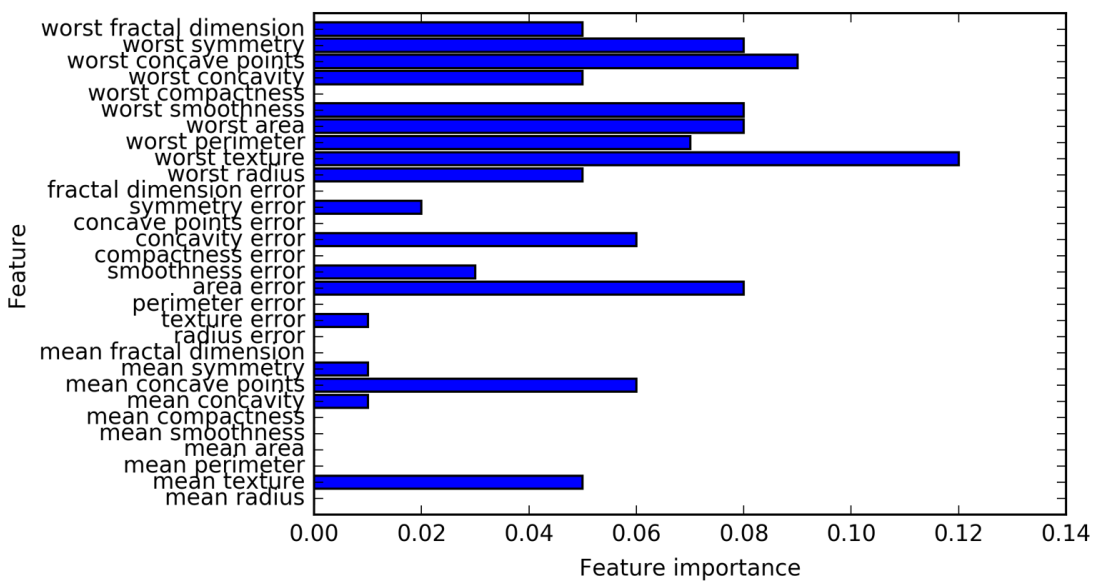
\includegraphics[scale=0.50]{../Imagen_Machine/ImportGradiente}
	\caption{Importancias de características calculadas a partir de un clasificador gradient boosted  que se ajusta a la data  cáncer de mama}
	\label{ImportGradiente}
\end{figure}


Podemos ver que la importancia de las características en gradient boosted,  son algo similar a la importancia de las características de los bosques aleatorios, aunque el gradient boosted ignoró por completo algunas de las características.\\

Dado que tanto en potenciación del gradiente   (gradient boosting)  como en bosques aleatorios se 
obtienen buenos resultados con datos similares, un enfoque común es probar primero en  bosques 
aleatorios, que funcionan con bastante solidez, muy robusto. Si los bosques aleatorios funcionan 
bien, pero el tiempo de predicción está en juego o es importante exprimir el último porcentaje de exactitud del modelo de aprendizaje automático, el aumento del gradiente generalmente ayuda.\\
calidad superior a la media

Si se quiere aplicar el gradient boosting a un problema de gran escala, tal vez  valer la pena
revisar el paquete {\ttfamily xgboost}\index{xgboost} y su interfaz Python, que al momento de la escritura
 es más rápido  que la implementación gradient boosting  en  {\ttfamily scikit-learn}   en muchos conjuntos de datos, y  {\ttfamily xgboost} es algunas veces es más fácil de ajustar.


\subsubsection{Fortalezas, debilidades y parámetros}

Los Árboles de decisión potenciados por gradiente o árboles de regresión potenciados se encuentran entre los modelos más potentes y ampliamente utilizados para el aprendizaje supervisado. Su principal inconveniente es que requieren un ajuste cuidadoso de los parámetros y pueden llevar mucho tiempo en su entrenamiento. De manera similar   otros modelos basados en árboles, el algoritmo funciona bien sin escalar y en una mezcla de  características binarias y continuas. Al igual que con otros modelos basados en árboles, por lo general no funciona bien  sobre datas  sparse de alta dimensión.\\

%  regresión del árbol de decisión potenciado

Los parámetros principales de los modelos de gradiente potenciado  son:  el número de árboles a usar en el modelo  {\ttfamily n\_estimators},  y  la taza de aprendizaje {\ttfamily learning\_rate} que controla el  grado en que  cada árbol correge los errores de los árboles anteriores.  Estos dos parámetros están altamente interconectados, ya que una  menor taza de aprendizaje {\ttfamily learning\_rate},  significa que se necesitan más árboles para construir un modelo de  complejidad similar. 

En contraste con los bosques aleatorios en donde un valor más alto  de \: {\ttfamily n\_estimators} es siempre mejor,  en el gradient boosting  un incremento de {\ttfamily n\_estimators} conduce a un modelo más complejo,  que puede conducir al sobreajuste. Una práctica común es ajustar el {\ttfamily n\_estimators}  dependiendo del   tiempo y la capacidad de memoria, y luego probar con diferentes  {\ttfamily learning\_rates}. \\	


Otro parámetro importante es la profundidad máxima  {\ttfamily max\_depth}, o como alternativa puede ser {\ttfamily max\_leaf\_nodes},  para reducir la  complejidad de cada árbol. Por lo general el parámetro {\ttfamily max\_depth} en los  modelos  gradient boosted,  se configuran con valores no más de cinco divisiones, es decir, valores bajos. \\
 
 
%  https://scikit-learn.org/stable/modules/model_evaluation.html

\subsection{Máquinas de soporte de vectores kernelized}\label{kenrelpag}

 %  máquinas de soporte vectorial  centralizadas,kernel\\

En  esta sección se estudia un modelo de aprendizaje  automatizado  supervisado,  llamado  Máquinas de soporte de vectores kernelized  (SVMs).  En la sección  dedicada a "{}Modelos lineales para clasificación"{}  en la página \pageref{Mlineales},  se introdujo el uso de máquinas de soporte de vectores  lineal (SVM) para la clasificación. Esta técnica de SVMs   es una extensión de SVM que permite modelos más complejos que definen otras curvas y no  simplemente rectas o hiperplanos  en el espacio de entrada. Más adelante se desarrolla un ejemplo donde resulta una elipse (figura \ref{LimitDesi3D}) como límite de decisión. 

Hay máquinas de soporte de vectores  para clasificación y regresión, sin embargo, en este texto nos limitaremos a la caso de clasificación, tal como se implementó en SVC. De manera análoga, los conceptos  se aplican al vector de soporte para regresión,   y se implementa en SVR.\\


La matemática detrás de las máquinas de soporte de vectores kernelized es un poco complicada y 
está más allá el alcance de este libro. Puede encontrar los detalles en el el Capítulo 1 del Libro: \href{https://web.stanford.edu/~hastie/ElemStatLearn//}{\color{vino} The Elements of Statistical Learning}
  de  Hastie,  Tibshirani, and Friedman’s. Sin embargo, 
trataremos  de darle sentido práctico a la idea del método.



\subsubsection{Modelos lineales y características no lineales}


Como se ve en la Figura \ref{SVM}, los modelos lineales pueden ser muy limitados en espacios
baja dimensión, como líneas rectas e hiperplanos que  tienen flexibilidad limitada. Una forma 
de hacer que un  modelo  un lineal sea más flexible es agregar más características, por ejemplo, agregar
interacciones o polinomios como características de entrada.\\


Ilustremos la idea con la data  sintética que se usó para visualizar la  "{}Importancia de la característica  en los árboles"{} en la página \pageref{ImpotCaract}  (Figura \ref{EtiquetArbol2}):

\begin{lstlisting}
In[76]: X, y = make_blobs(centers=4, random_state=8)
        y = y % 2
        mglearn.discrete_scatter(X[:, 0], X[:, 1], y)
        plt.xlabel("Feature 0")
        plt.ylabel("Feature 1")
\end{lstlisting}


\begin{figure}[h!]
	\centering
	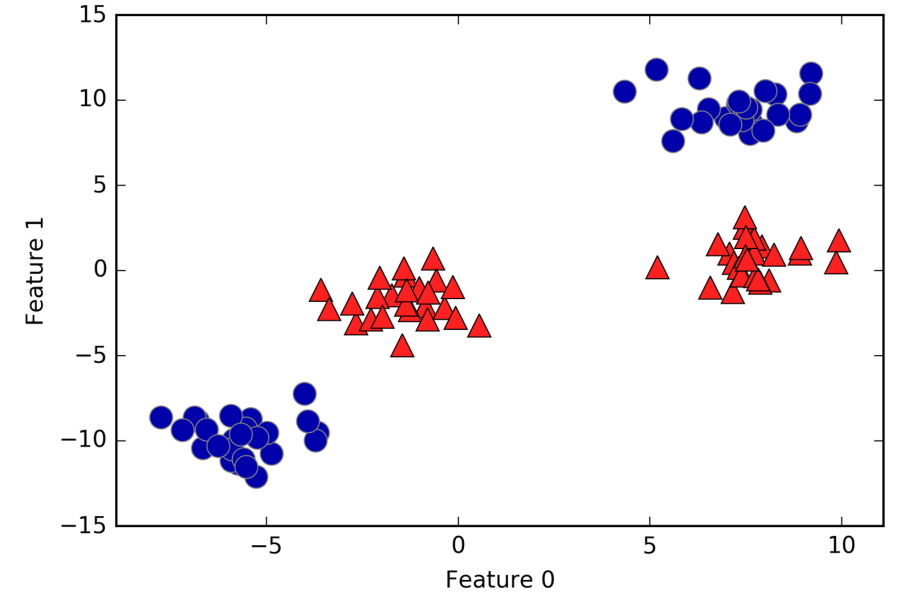
\includegraphics[scale=0.50]{../Imagen_Machine/Conjunto2D}
	\caption{Data con dos clases, en el que las clases no son linealmente separables}
	\label{Conjunto2D}
\end{figure}

Un modelo lineal para  clasificar esta data, sólo puede separar los puntos usando una línea recta, y no será
capaz de hacer un buen trabajo en este conjunto de datos (ver Figura \ref{SVMLineal}):\\


\begin{lstlisting}
In[77]: from sklearn.svm import LinearSVC
	linear_svm = LinearSVC().fit(X, y)
	
	mglearn.plots.plot_2d_separator(linear_svm, X)
	mglearn.discrete_scatter(X[:, 0], X[:, 1], y)
	plt.xlabel("Feature 0")
	plt.ylabel("Feature 1")
\end{lstlisting}


Observe lo que sucede  al expandir el conjunto de características de entrada, por ejemplo, agregando también  {\ttfamily feature1 ** 2}, el cuadrado de la segunda característica, como una nueva característica.  Ahora, en lugar de representar cada punto de datos como un punto bidimensional (feature0, feature1), lo representamos como un punto tridimensional (feature0, feature1, feature1 ** 2). Es importante notar que la elección de  esta característica  se hizo únicamente con  fines  para la ilustración, esta elección no tiene alguna  particularida importante.   Ahora, esta nueva representación se ilustrada en la figura \ref{Tridimensional}, un diagrama de dispersión tridimensional:


\begin{figure}[h!]
	\centering
	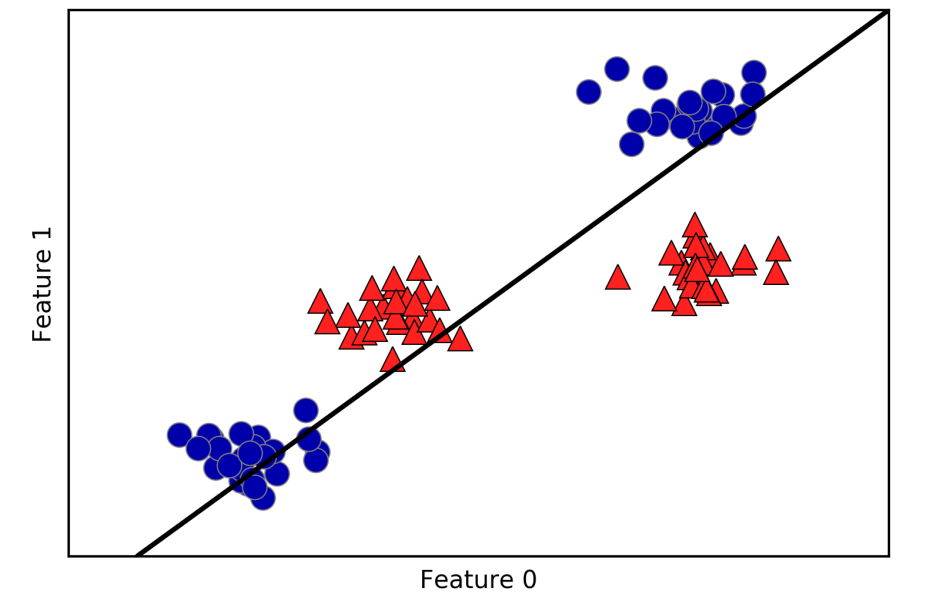
\includegraphics[scale=0.50]{../Imagen_Machine/SVMLineal}
	\caption{Límite de decisión encontrado por un SVM lineal}
	\label{SVMLineal}
\end{figure}



\begin{lstlisting}
In[78]: # Anade el cuadrado de la primera caracteristica
	X_new = np.hstack([X, X[:, 1:] ** 2])    #  apila horizontal
	
	from mpl_toolkits.mplot3d import Axes3D, axes3d
	figure = plt.figure()
	# visualize in 3D
	ax = Axes3D(figure, elev=-152, azim=-26)
	# plot first all the points with y == 0, then all with y == 1
	mask = y == 0
	ax.scatter(X_new[mask, 0], X_new[mask, 1], X_new[mask, 2], c='b',
	           cmap=mglearn.cm2, s=60)
	ax.scatter(X_new[~mask, 0], X_new[~mask, 1], X_new[~mask, 2], 
	            c='r', marker='^', cmap=mglearn.cm2, s=60)
	ax.set_xlabel("feature0")
	ax.set_ylabel("feature1")
	ax.set_zlabel("feature1 ** 2")
\end{lstlisting}



En la nueva representación de la data, ahora es posible separar las dos clases usando un modelo 
lineal, un plano en tres dimensiones. Podemos confirmar esto ajustando un modelo lineal a la data aumentada (ver Figura \ref{HiperPlano}): 

\begin{lstlisting}
In[79]: linear_svm_3d = LinearSVC().fit(X_new, y)
	coef      =  linear_svm_3d.coef_.ravel() 
	intercept =  linear_svm_3d.intercept_
	# show linear decision boundary
	figure = plt.figure()
	ax = Axes3D(figure, elev=-152, azim=-26)
	xx = np.linspace(X_new[:, 0].min() - 2, X_new[:, 0].max() + 2, 50)
	yy = np.linspace(X_new[:, 1].min() - 2, X_new[:, 1].max() + 2, 50)
	
	XX, YY = np.meshgrid(xx, yy)
	ZZ = (coef[0] * XX + coef[1] * YY + intercept) / -coef[2]
	ax.plot_surface(XX, YY, ZZ, rstride=8, cstride=8, alpha=0.3)
	ax.scatter(X_new[mask, 0], X_new[mask, 1], X_new[mask, 2], 
	           c='b', cmap=mglearn.cm2, s=60)
	ax.scatter(X_new[~mask, 0], X_new[~mask, 1], X_new[~mask, 2],
	           c='r', marker='^', cmap=mglearn.cm2, s=60)

	ax.set_xlabel("feature0")
	ax.set_ylabel("feature1")
	ax.set_zlabel("feature0 ** 2")
\end{lstlisting}





\begin{figure}[h!]
	\centering
	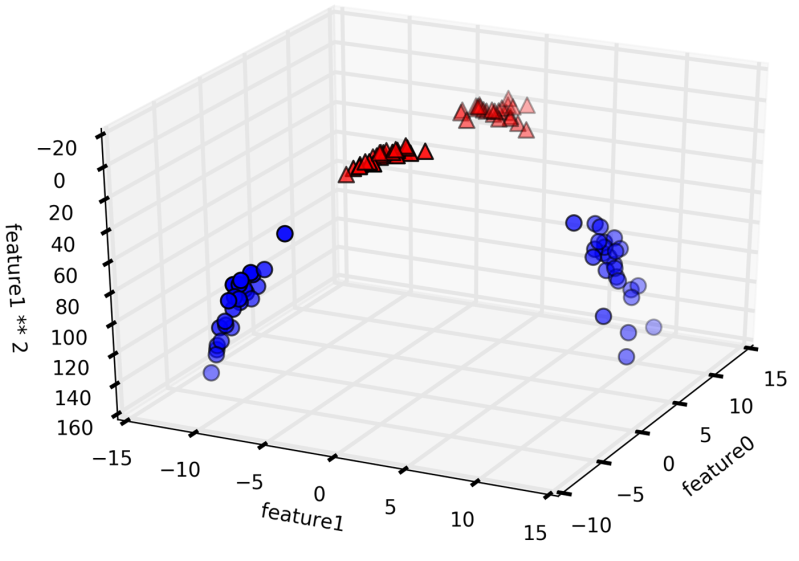
\includegraphics[scale=0.50]{../Imagen_Machine/Tridimensional}
	\caption{Expansión del conjunto de datos de la Figura \ref{SVMLineal}, 
		creada añadiendo una tercera característica derivada de la característica 1.}
	\label{Tridimensional}
\end{figure}







\begin{figure}[h!]
	\centering
	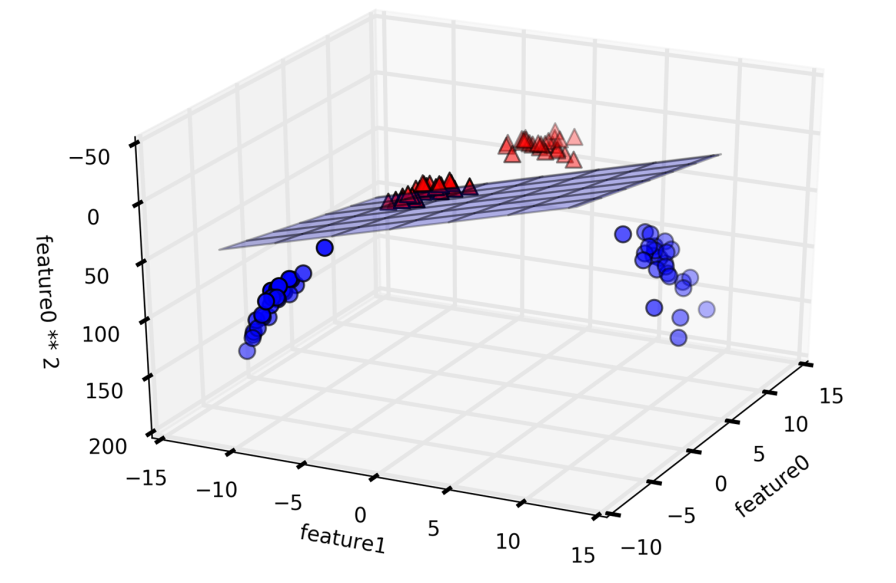
\includegraphics[scale=0.50]{../Imagen_Machine/HiperPlano}
	\caption{Límite de decisión encontrado por un SVM lineal en el conjunto de datos tridimensionales expandidos.}
	\label{HiperPlano}
\end{figure}
 
 
  Luego de este cambio, en el modelo lineal SVM  en función de las dos características originales, el límite de decisión  ya no es lineal, ya no se comporta como una linea recta, sino más bien una elipse, como se puede ver en en el gráfico que se muestra en la Figura \ref{LimitDesi3D}:\\

\begin{lstlisting}
In[80]: ZZ = YY ** 2
	dec = linear_svm_3d.decision_function(np.c_[XX.ravel(),
	                                       YY.ravel(), ZZ.ravel()])
	plt.contourf(XX, YY, dec.reshape(XX.shape),
	             levels=[dec.min(), 0, dec.max()], cmap=mglearn.cm2, 
	             alpha=0.5)
	mglearn.discrete_scatter(X[:, 0], X[:, 1], y)
	plt.xlabel("Feature 0")
	plt.ylabel("Feature 1")
\end{lstlisting}


\begin{figure}[h!]
	\centering
	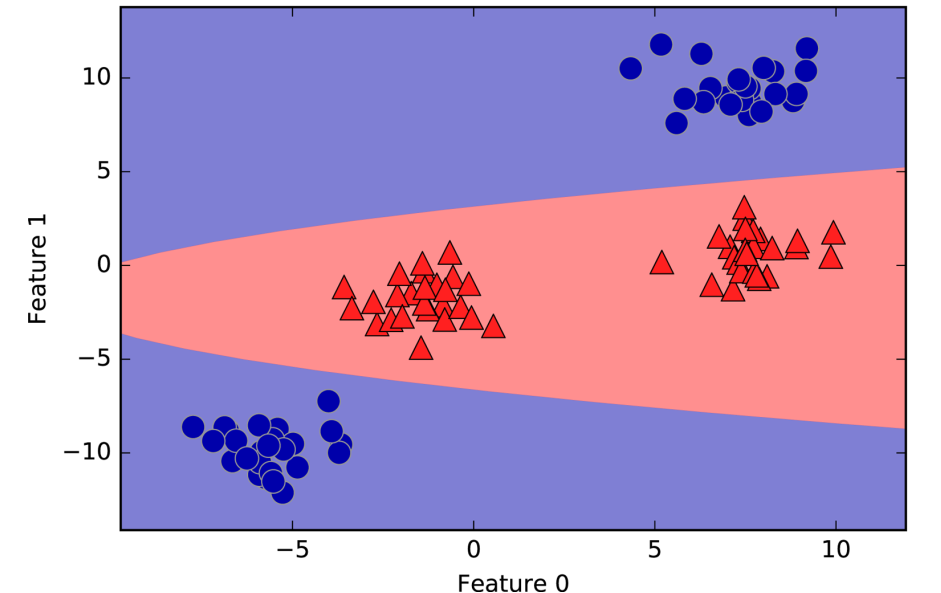
\includegraphics[scale=0.50]{../Imagen_Machine/LimitDesi3D}
	\caption{El límite de decisión de la Figura \ref{HiperPlano} en función de las dos características originales}
	\label{LimitDesi3D}
\end{figure}



\subsubsection{El truco del kernel}

La idea aquí es  añadir características no lineales a la data  para la representación,  
y de  esta forma se puede lograr que  los modelos lineales sean  más potentes.  Sin embargo, a menudo no 
sabemos qué características añadir, y la adición de muchas características (como todas las
 interacciones posibles en un espacio de características de 100 dimensiones) puede hacer  el costo de computación muy alto. Afortunadamente, hay un truco matemático inteligente que le permite el  aprendizaje a un clasificador en un espacio de dimensiones más altas,  sin ejecutar realmente los nuevos calculos. Este truco conoce como el truco del kernel; y trabaja calculando directamente la distancia (más precisamente, los productos escalares) de los puntos de datos para la representación de las características expandidas, sin calcular realmente la expansión.\\
 
 
 % Afortunadamente, hay un truco matemático inteligente que nos permite aprender un clasificador en un espacio de dimensiones superiores sin realmente computar la nueva, posiblemente muy grande representación
  
%  Luckily, there is   a clever mathematical trick that allows us to learn a classifier in a higher-dimensional   space without actually computing the new, possibly very large representation
  
  
 Hay dos maneras de mapear sus datos en un espacio de dimensiones superiores que se utilizan comúnmete con máquinas de soporte de vectores: una se refiere al kernel polinomial, que calcula todos los polinomios posibles hasta un cierto grado de las características originales (como {\ttfamily feature1**2 * feature2 ** 5}); y el otro es el kernel de la función de base radial   (radial basis function kernel,  RBF), también conocido como  el kernel Gaussiano.  El  kernel Gaussiano es un poco más difícil de explicar, ya que corresponde a un espacio de características de dimensiones infinitas. Una manera de explicar el  kernel Gaussian es considerar todos los polinomios posibles de todos los grados, pero la importancia de las características disminuyen para grados muy altos (expansión de Taylor).\\


En la práctica, los detalles matemáticos de fondo del  kernel  SVM no son tan importantes al análisis, sin embargo,  una SVM con un kernel RBF toma una decisión que se puede resumir fácilmente; para comprender esta idea explicamos en la  siguiente sección. 

\subsubsection{Comprendiendo el proceso de SVMs}

Durante el entrenamiento, el SVM aprende la importancia de cada uno de los puntos de datos del entrenamiento para representar el límite de decisión entre las dos clases; generalmente  sólo un subconjunto del entrenamiento es importartante para definir el límite de decisión: y son los datos que se encuentran en la frontera entre las clases. Estos se llaman soporte de vectores, que dan su nombre a la máquina de soporte de vectores.


 Para hacer una predicción de un nuevo punto, la distancia a cada uno de los  soporte de vectores es medida. Se toma una decisión de clasificación basada en las distancias al vector de soporte, y a la importancia de los soporte de vectores que fuerón aprendiendo durante el entrenamiento (almacenados en el atributo  {\ttfamily dual\_coef\_} de SVC).\\


La distancia entre puntos de la data es medido por el kernel Gaussiano: 


\begin{equation}\label{gausss}
 k_{rbf}(x_{1}, x_{2}) = exp (\gamma \|x_{1} - x_{2}\|^{2} ). 
 \end{equation} Aquí, $x_{1}$  y  $x_{2} $  son puntos de la data, $\| x_{1} - x_{2} \| $ denota distancia Euclidean, y $\gamma$ (gamma) es un parámetro que controla el ancho del kernel Gaussian.\\


 La Figura \ref{KernelGausiano1} muestra el resultado del entrenamiento de una máquina de vector de soporte en un conjunto de datos bidimensional con dos clases. El límite de decisión se muestra como la curva  en negro, y los vectores de suporte son puntos más grandes con el contorno ampliamante marcado. El siguiente código genera el gráfico de entrenanar  un SVM en la dataset de falsificación de datos (forge dataset):

\begin{lstlisting}
In[81]: from sklearn.svm import SVC
	X, y = mglearn.tools.make_handcrafted_dataset()
	svm = SVC(kernel='rbf', C=10, gamma=0.1).fit(X, y)
	mglearn.plots.plot_2d_separator(svm, X, eps=.5)
	mglearn.discrete_scatter(X[:, 0], X[:, 1], y)
	# plot support vectors
	sv = svm.support_vectors_
	# class labels of support vectors are given by the sign 
	# of the dual coefficients
	sv_labels = svm.dual_coef_.ravel() > 0
	mglearn.discrete_scatter(sv[:, 0], sv[:, 1], sv_labels, 
	                         s=15, markeredgewidth=3)
	plt.xlabel("Feature 0")
	plt.ylabel("Feature 1")	
\end{lstlisting}


\begin{figure}[h!]
	\centering
	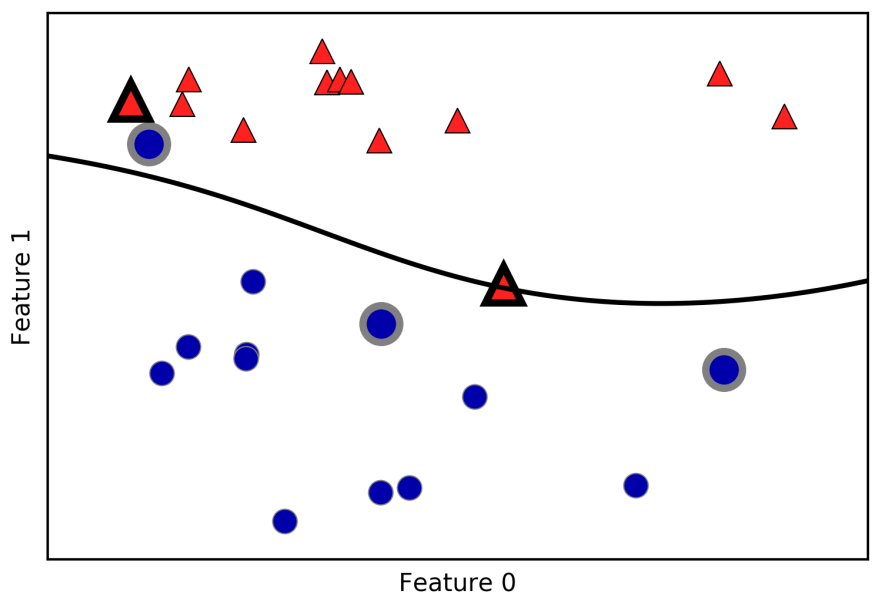
\includegraphics[scale=0.50]{../Imagen_Machine/KernelGausiano1}
	\caption{Límite de decisión y soporte de vectores encontrados por un SVM con el kernel Gaussiano}
	\label{KernelGausiano1}
\end{figure}

En este caso, el SVM produce un límite de decisión  más suave y no lineal  (no es una línea recta). 
Aquí se ajustaron dos parámetros: el  $C = 10 $ y el  gamma = 0.1.  A  continuacón
 se trata con más detalle este ajuste.


\subsubsection{Ajuste de los parámetros de SVM}

El parámetro gamma es el que se muestra en la fórmula \ref{gausss} dada en la sección anterior, que controla el ancho del kernel Gaussiano; determina la escala de lo que significa para los puntos estar uno al lado del otro (estar cerca uno del otro).  Y  $C$  es un parámetro de regularización, similar al utilizado en los modelos lineales, y límita la importancia de cada punto  {\ttfamily dual\_coef\_}.\\

En la Figura \ref{gama2} podemos ver lo que sucede cuando variamos estos parámetros:\\

\begin{lstlisting}  % [frame=single]	

In[82]: fig, axes = plt.subplots(3, 3, figsize=(15, 10))
   
        for ax, C in zip(axes, [-1, 0, 3]):
            for a, gamma in zip(ax, range(-1, 2)):
            mglearn.plots.plot_svm(log_C=C, log_gamma=gamma, ax=a)
           
        axes[0, 0].legend(["class 0", "class 1", "sv class 0", "sv class 1"],
                           ncol=4, loc=(.9, 1.2))
  
\end{lstlisting}

 
 De izquierda a derecha, aumentamos el valor del parámetro gamma de 0,1 a 10. Un pequeño gamma significa un gran radio para el kernel Gaussiano, lo que significa que muchos puntos se consideran cercanos.
Esto se refleja en límites de decisión muy suaves a la izquierda, y límites que se centran más en puntos individuales más a la derecha.  Un valor bajo de gamma significa que el límite de decisión variará lentamente, lo que produce un modelo de baja complejidad, mientras que un valor alto de gamma produce un modelo más complejo. 
\begin{figure}[h!]
	\centering
	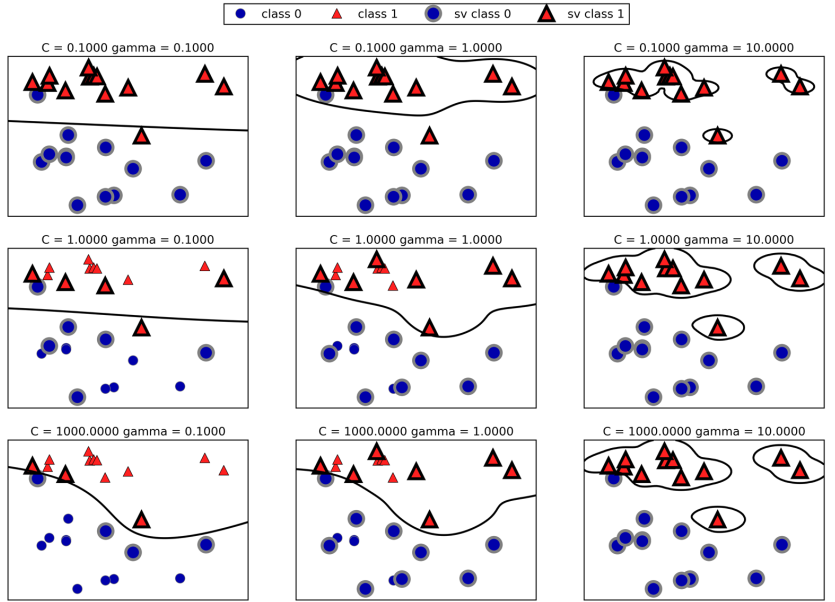
\includegraphics[scale=0.75]{../Imagen_Machine/gama2}
	\caption{Los límites de decisión y los vectores del soporte para los  diferentes  ajustes  de los  parámetros $C $ y  gamma}
	\label{gama2}
\end{figure} Y de arriba a abajo, aumentamos el parámetro C de 0.1 a 1000. Al igual que con los modelos lineales, un pequeño C significa un modelo muy restringido, donde cada punto de datos sólo puede tener una influencia muy limitada. Se puede ver que en la parte superior izquierda el límite de decisión parece casi lineal, con  puntos mal clasificados con poca o ninguna influencia sobre la línea. Incrementando $C$ como se muestra en la parte inferior derecha, permite que esos puntos tengan una mayor influencia sobre el modelo y hacen  del límite de decisión una curva suave  para clasificarlos correctamente.\\


Ahora aplicamos la técnica de SVM  con el kernel  gaussiano  al conjunto de datos de Cáncer de Mama (Breast Cancer). Con los parámetros por defecto,  $C=1 $  y gamma $= 1/n${\ttfamily \_features}:


\begin{lstlisting}
In[83]: X_train, X_test, y_train, y_test = train_test_split(
	    cancer.data, cancer.target, random_state=0)
	    
	svc = SVC()
	svc.fit(X_train, y_train)
	
	print("Accuracy on training set: {:.2f}".format(
	       svc.score(X_train, y_train)))
	print("Accuracy on test set: {:.2f}".format(
	       svc.score(X_test, y_test)))

Out[83]:

	Accuracy on training set: 1.00
	Accuracy on test set: 0.63

\end{lstlisting}


El modelo resultó con un puntaje de exactitud perfecta sobre el conjunto de entrenamiento, lo que indica un sobreajuste muy alto, mientras que la exactitud en el conjunto de prueba es de 63\%. Aunque los SVMs generalmente  funcionan bastante bien, estos son muy sensibles a la configuración de los parámetros y a la escala de los datos. En particular, requieren que todas las características varíen en una escala similar. Veamos los valores mínimos y máximos para cada característica, graficada en log-space (Figura \ref{RangosLog}):

\begin{lstlisting}
In[84]: plt.plot(X_train.min(axis=0), 'o', label="min")
	plt.plot(X_train.max(axis=0), '^', label="max")
	plt.legend(loc=4)
	plt.xlabel("Feature index")
	plt.ylabel("Feature magnitude")
	plt.yscale("log")

\end{lstlisting}


\begin{figure}[h!]
	\centering
	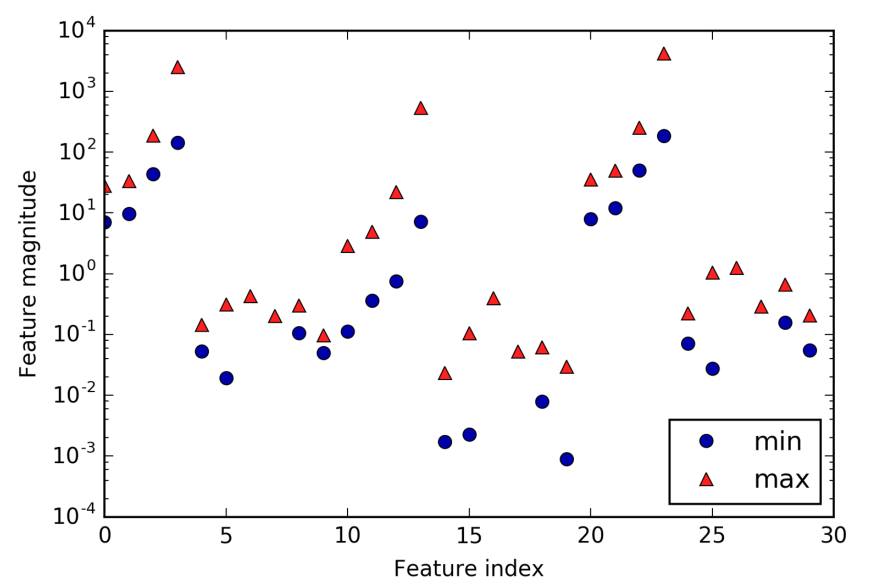
\includegraphics[scale=0.50]{../Imagen_Machine/RangosLog}
	\caption{Rangos de características para el conjunto de datos de cáncer de mama (el eje $y$ en escala logaritmica)}
	\label{RangosLog}
\end{figure}


A partir de esta gráfica, podemos determinar que las características en la data Cáncer de Mama tienen órdenes de magnitud completamente diferentes.  Esto puede ser un problema para otros modelos (como los modelos lineales), pero tiene efectos devastadores para el kernel SVM. Examinemos algunas maneras de tratar  este asunto.


\subsubsection{Preprocesamiento de datos para SVMs}


Una forma de resolver este problema es volver a reescalar  cada característica para que estén aproximadamente en la misma escala.  Un método común de re-escalar  para kernel SVMs, conciste en escalar los datos de tal manera que todas las características estén entre 0 y 1.  En el Capítulo \ref{Cap3} veremos cómo hacerlo usando el método de preprocesamiento Minmaxscaler, donde daremos más detalles. Por ahora, lo haremos esto "{}a mano":

\begin{lstlisting}  

In[85]: # compute the minimum value per feature on the training set
        min_on_training = X_train.min(axis=0)
        # compute the range of each feature (max - min) on the training set
        range_on_training = (X_train - min_on_training).max(axis=0)
   
        # subtract the min, and divide by range
        # afterward, min=0 and max=1 for each feature
        X_train_scaled = (X_train - min_on_training) / range_on_training
        print("Minimum for each feature\n{}".format(
               X_train_scaled.min(axis=0)))
        print("Maximum for each feature\n {}".format(
               X_train_scaled.max(axis=0)))

Out[85]:

    Minimum for each feature
    [ 0.  0.  0.  0.  0.  0.  0.  0.  0.  0.  0.  0.  0.  0.  0.  0.  0.  0.
      0.  0.  0.  0.  0.  0.  0.  0.  0.  0.  0.  0.]
    Maximum for each feature
    [ 1.  1.  1.  1.  1.  1.  1.  1.  1.  1.  1.  1.  1.  1.  1.  1.  1.  1.
      1.  1.  1.  1.  1.  1.  1.  1.  1.  1.  1.  1.]


In[86]: # use THE SAME transformation on the test set,
        # using min and range of the training set (see Chapter 3 for details)
        X_test_scaled = (X_test - min_on_training) / range_on_training
   
In[87]: svc = SVC()
        svc.fit(X_train_scaled, y_train)
   
        print("Accuracy on training set: {:.3f}".format(
               svc.score(X_train_scaled, y_train)))
        print("Accuracy on test set: {:.3f}".format(
               svc.score(X_test_scaled, y_test)))
   
Out[87]:
  
    Accuracy on training set: 0.948
    Accuracy on test set: 0.951


\end{lstlisting}



¡Escalando los datos hace una gran diferencia! Ahora nos encontramos en un régimen de subajuste, 
en el que el rendimiento del entrenamiento y el conjunto de prueba son muy similares, pero menos próximos al 100 \%. A partir de aquí, podemos tratar de aumentar ya sea C o gamma para adaptarse a un modelo más complejo. Por ejemplo:\\


\begin{lstlisting}
In[88]: svc = SVC(C=1000)
	svc.fit(X_train_scaled, y_train)
	
	print("Accuracy on training set: {:.3f}".format(
	       svc.score(X_train_scaled, y_train)))
	print("Accuracy on test set: {:.3f}".format(
	       svc.score(X_test_scaled, y_test)))

Out[88]:
	Accuracy on training set: 0.988
	Accuracy on test set: 0.972
\end{lstlisting}


\noindent Aquí, el aumento de C nos permite mejorar significativamente el modelo, lo que resulta en un 97.2\%
exactitud.


\subsubsection{Fortalezas, debilidades y parámetros}

Las máquinas de soporte de vectores Kernelized\index{soporte de vectores Kernelized} son modelos potentes y funcionan bien en una variedad
 de conjuntos de datos. Las SVMs permiten límites de decisión complejos, incluso si los datos solo tienen pocas características. Funcionan bien en datos de baja y alta dimensión (es decir, con pocas y muchas características), pero puede generar cierta dificultad con el número de muestras; correr un SVM con datos de tamaño hasta de 10.000 muestras podría funcionar bien, pero trabajar con conjuntos de datos de tamaño 100.000 o más, pueden convertirse en un desafío en términos de tiempo de ejecución y uso de memoria.\\


Otro inconveniente de los SVMs es que requieren un cuidadoso tratamiento previo (preprocesamiento)  de los datos y ajuste de los parámetros. Esta es la razón por la que hoy en día la mayoría de la gente utiliza modelos basados en árboles, como bosques aleatorios o potenciación de gradientes (que requieren poco o ningún proceso previo) en muchas aplicaciones.   Además, los modelos SVM son difíciles de inspeccionar; puede ser difícil entender por qué  hizo una predicción en particular, y podría ser difícil explicar el modelo a los inexpertos.\\

Aún así, podría valer la pena probar SVMs, especialmente si todas sus características estan  representadas
en unidades de medidas similares (por ejemplo, todas son intensidades de píxeles) y están en 
escala  similar.\\

Los parámetros importantes en el  kernel SVMs  son el parámetro de regularización C, la
elección del kernel, y los parámetros específicos del kernel.  Aunque principalmente se enfoca en el  kernel  kernel Gaussiano (RBF), en {\ttfamily scikit-learn}  hay otras opciones disponibles.  El  kernel RBF  tiene un sólo   que es el inverso del ancho del  kernel Gaussiano, el  parámetro el gamma.   Los  parámetro gamma y C controlan la complejidad del modelo, con valores grandes en cualquier de los dos, resulta un modelo más complejo. Por lo tanto, deben configurarse bien los dos los parámetros que  generalmente resulta altamente correlacionados; es decir,  deben cofigurarse juntos ($C$ y gamma).


\subsection{Redes Neuronales (Aprendizaje Profundo)}

Una familia de algoritmos conocidos como redes neuronales\index{redes neuronale}, se han visto recientemente en un renacimiento bajo el nombre de \: "{}Aprendizaje Profundo" \:(deep learnig). El aprendizaje profundo ofrece una  gran promesa en muchas aplicaciones de aprendizaje automático,  sus algoritmos   se adaptan generalmente a un caso de uso muy específico.  Aquí sólo discutiremos algunos métodos relativamente simples, como  los perceptores multicapa o multilayer para la clasificación y la regresión, que pueden servir como punto de partida para  comenzar a involucrarse con métodos de aprendizaje profundo, con mayor nivel.   Los perceptores Multilayer (MLPs)   también se conocen como \:  "{}Redes Neuronales de feed-forward"  {}\:(vanilla), o sólo redes neuronales. %    que se las alimentan adelante redes de nervios

% El perceptrón es una red neuronal artificial (RNA) formada por múltiples capas, de tal manera que tiene capacidad para resolver problemas que no son linealmente separables, lo cual es la principal limitación del perceptrón (también llamado perceptrón simple).


\subsubsection{El modelo de red neuronal}

Los perceptores Multilayer (MLPs)  pueden verse como generalización de modelos lineales que realizan múltiples etapas de procesamiento para llegar a una decisión.\\

Recuerde que la predicción para un regresor lineal esta dada como:

  \[  \hat{y} = w[0] * x[0] + w[1] * x[1] + ... + w[p] * x[p] + b \]

En palabras simple, $\hat{y}$  es una suma ponderada de las características de entrada $x[0]$ a $x[p]$, 
ponderada por los coeficientes aprendidos $w[0]$ a $w[p]$ .\\

En la Figura \ref{RegresLogis2-44} se ilustrar  gráficamente esta idea:

\begin{lstlisting}  % [frame=single]	

In[89]: display(mglearn.plots.plot_logistic_regression_graph())

\end{lstlisting}


\begin{figure}[h!]
	\centering
	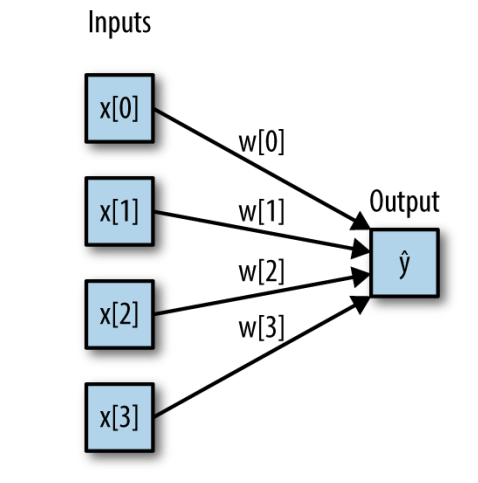
\includegraphics[scale=0.50]{../Imagen_Machine/RegresLogis2-44}
	\caption{Visualización de la regresión logística, donde las características de entrada y las predicciones  se muestran como nodos, y los coeficientes son conexiones entre los nodos}
	\label{RegresLogis2-44}
\end{figure}


Aquí, cada nodo de la izquierda representa una característica de entrada, las líneas de conexión representan los coeficientes aprendidos, y el nodo de la derecha representa la salida, que es una suma ponderada de las entradas.\\ 


En un MLP, este proceso de cálculo de sumas ponderadas se repite varias veces, primero computando unidades ocultas que representan una etapa de procesamiento intermedia, y que luego  se combinan usando  nuevamente  sumas ponderadas para obtener el resultado final (Figura \ref{Layeoculas}):\\

\begin{lstlisting}  % [frame=single]	

In[90]: display(mglearn.plots.plot_single_hidden_layer_graph())

\end{lstlisting}

\begin{figure}[h!]
	\centering
	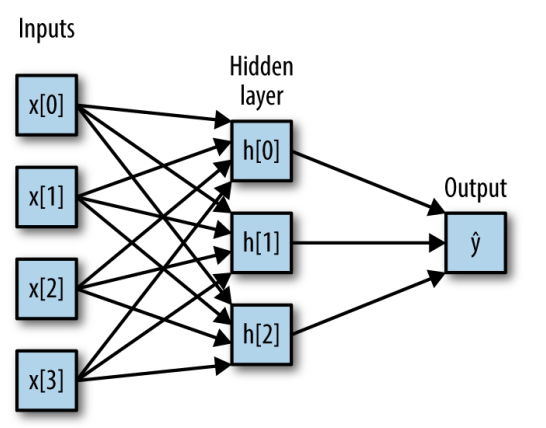
\includegraphics[scale=0.50]{../Imagen_Machine/Layeocultas}
	\caption{Ilustración de perceptrón multicapa con una única capa oculta}
	\label{Layeoculas}
\end{figure} Este modelo tiene muchos más coeficientes (también llamados pesos o ponderaciones) para aprender,  hay uno
entre cada entrada y cada unidad oculta (que forman la capa oculta), y uno entre cada unidad en la capa oculta y la salida.\\


Calcular una serie de sumas ponderadas es matemáticamente lo mismo que calcular sólo
una suma ponderada;    para que este modelo sea realmente más poderoso que un modelo lineal,
necesitamos un truco extra. Después de calcular una suma ponderada para cada unidad oculta, una función no lineal se aplica al resultado, generalmente la  rectificadora no lineal  (también conocido como unidad  rectificada  lineal o relu) o las tangetes hiperbólicos (tanh).   El resultado de esta función es entonces usado en la suma ponderada que calcula la salida  $ \hat{y}$.   Las dos  funciones se visualizan en la Figura \ref{Tangete}.    El relu corta valores por debajo de cero, mientras que la tanh se satura  hasta –1,  para valores de entrada bajos;  y    para valores de entrada altos el  $+1$. Otras funciones no lineales permite a la red neuronal aprender funciones mucho  más  complicadas,  de lo que  podría hacer un modelo lineal:\\


\begin{lstlisting}   
In[91]: line = np.linspace(-3, 3, 100)
        plt.plot(line, np.tanh(line), label="tanh")
        plt.plot(line, np.maximum(line, 0), label="relu")   
        plt.legend(loc="best")
        plt.xlabel("x")
        plt.ylabel("relu(x), tanh(x)")
	
\end{lstlisting}


\begin{figure}[h!]
	\centering
	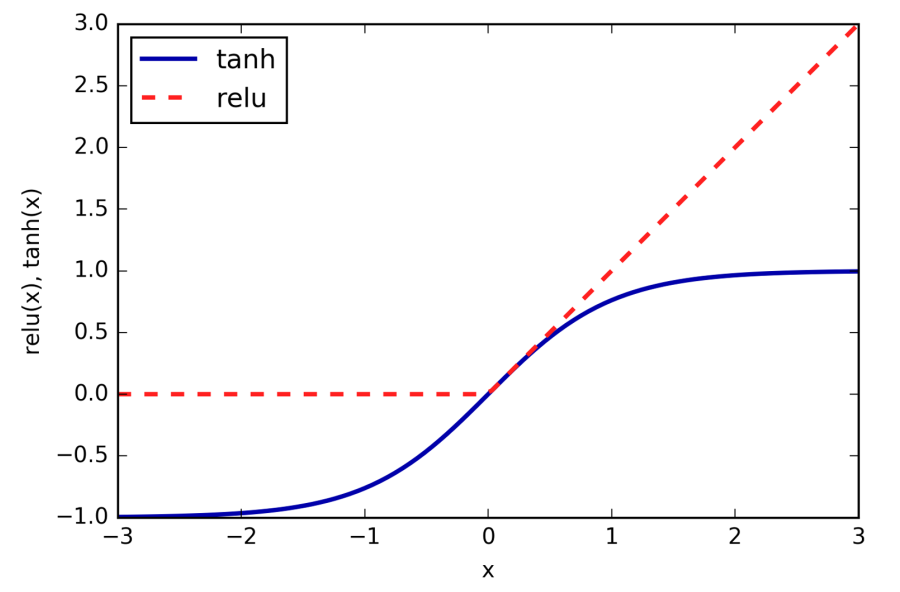
\includegraphics[scale=0.50]{../Imagen_Machine/Tangete}
	\caption{La función de activación tangente hiperbólica y la función de activación lineal 
		rectificada.}
	\label{Tangete}
\end{figure}


Para  red neuronal representada en la Figura \ref{Layeoculas}, la fórmula completa para 
la cálculo $\hat{y}$  en el caso de regresión sería (cuando se utiliza  tanh, no linealidad):\\
{\scriptsize{
\[
\begin{array}{l c l}
	h[0] & = &  tanh (w [0, 0] * x [0] + w [1, 0] * x [1] + w [2, 0] * x [2] + w [3, 0] * x [3]) \\
	h[1] & = &  tanh (w [0, 0] * x [0] + w [1, 0] * x [1] + w [2, 0] * x [2] + w [3, 0] * x [3]) \\
	h[2] & = &  tanh (w [0, 0] * x [0] + w [1, 0] * x [1] + w [2, 0] * x [2] + w [3, 0] * x [3])\\
	\hat{y}& =& v [0] * h [0] + v [1] * h [1] + v [2] * h [2] 
\end{array} \\
\]
}}  Aquí, $w$ son los pesos entre la entrada $x$ y la capa oculta   $h$ (hidden layer), y  $ v $ son los
pesos entre la capa oculta $h$ y la salida $\hat{y}$. Los pesos $v$ y $w$ se aprenden
a partir de los datos, $x$ son las características de entrada, $\hat{y}$ es la salida calculada  y la $h$ son cálculos  intermedios. \\ 

Un parámetro importante que debe configurar el usuario es el número
de nodos en la capa oculta. Este puede ser tan pequeño como 10 para conjuntos de datos  muy pequeños o simples, y tan grande como 10.000 para data  muy complejas o muy grandes. También es posible agregar más
capas ocultas, como se muestra en la Figura \ref{Perceptron}:


\begin{lstlisting}  % [frame=single]	

In[92]: mglearn.plots.plot_two_hidden_layer_graph()

\end{lstlisting}


\begin{figure}[h!]
	\centering
	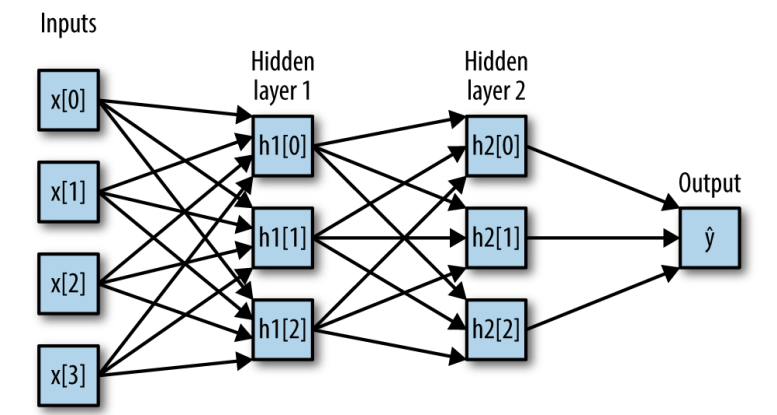
\includegraphics[scale=0.50]{../Imagen_Machine/Perceptron}
	\caption{Un perceptrón con dos capas ocultas, multicapa.}
	\label{Perceptron}
\end{figure}


Tener  redes neuronales grandes  compuestas de muchas de estas capas de cálculo computacinal es lo que inspiró el término "{}aprendizaje profundo".

\subsubsection{Ajuste de redes neuronales}

 Analicemos  el funcionamiento del perceptor multilayer MLP, aplicando el  {\ttfamily Mlpclassifier} sobre la dataset {\ttfamily two\_moons}  que se  usó anteriormente en este capítulo. Los resultados se muestran en la figura \ref{100ocultos}:\\


\begin{lstlisting}  % [frame=single]
	
In[93]: from sklearn.neural_network import MLPClassifier
	from sklearn.datasets import make_moons
   
   	 X, y = make_moons(n_samples=100, noise=0.25, random_state=3)
   
   	 X_train, X_test, y_train, y_test = train_test_split(X, y, 
   	                                                     stratify=y,
                                                         random_state=42)	
                                                 							   
   	 mlp = MLPClassifier(solve='lbfgs',
   	                      random_state=0).fit(X_train, y_train)
   	 mglearn.plots.plot_2d_separator(mlp, X_train, fill=True, alpha=.3)
   	 mglearn.discrete_scatter(X_train[:, 0], X_train[:, 1], y_train)
   	 plt.xlabel("Feature 0")
   	 plt.ylabel("Feature 1")
   
\end{lstlisting}



\begin{figure}[h!]
	\centering
	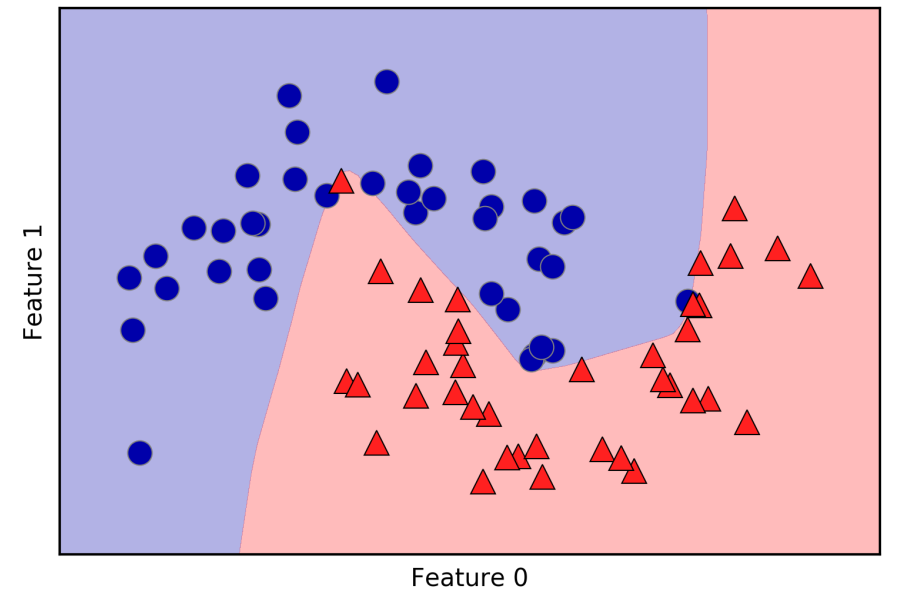
\includegraphics[scale=0.50]{../Imagen_Machine/100ocultos}
	\caption{Límite de decisión aprendido por una red neural con 100 unidades ocultas en el conjunto de datos \ttfamily{two\_moons}}
	\label{100ocultos}
\end{figure}

Como se puede ver, la red neuronal aprendió un límite de decisión relativamente suave y no lineal. Esto se logró empleando el  algoritmo {\ttfamily algorithm =  '\!lbfgs'}, que discurá más adelante.\\

Por defecto, el MLP usa 100 nodos ocultos, que en este caso es demasiado  para esta  pequeña  dataset.
Podemos reducir el número (el cual reduce la complejidad del modelo) y todavía podemos tener un buen resultado ( ver figura \ref{10nodos}):

lbfgs
\begin{lstlisting}	
In[94]:	mlp = MLPClassifier(solve='lbfgs', random_state=0,
                            hidden_layer_sizes=[10])
        mlp.fit(X_train, y_train)
        mglearn.plots.plot_2d_separator(mlp, X_train, fill=True, 
                                        alpha=.3)
        mglearn.discrete_scatter(X_train[:, 0], X_train[:, 1], y_train)
        plt.xlabel("Feature 0 ")
        plt.ylabel("Feature 1 ")

\end{lstlisting}	


\begin{figure}[h!]
	\centering
	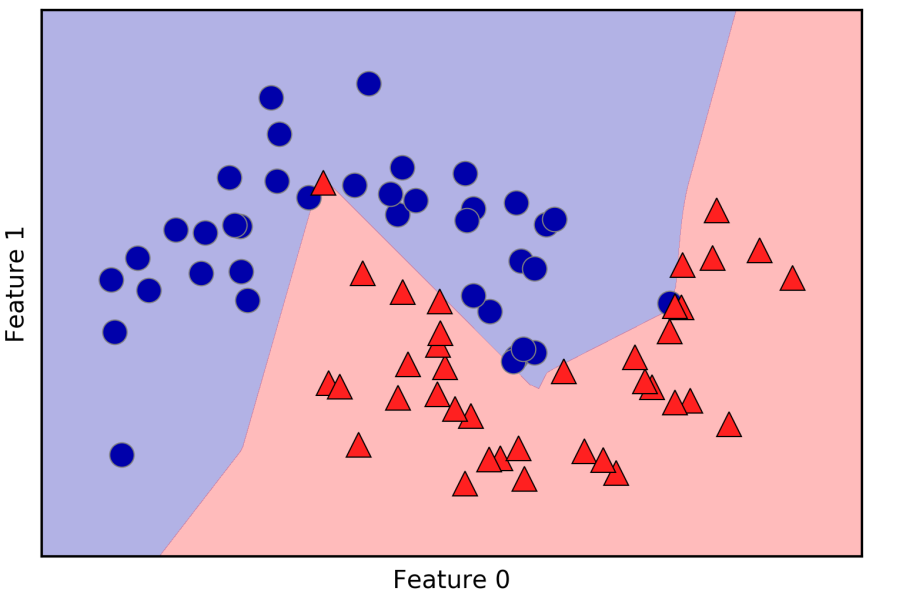
\includegraphics[scale=0.50]{../Imagen_Machine/10nodos}
	\caption{Límite de decisión aprendido por una red neural con 10 unidades ocultas en la dataset  \ttfamily{two\_moons}}
	\label{10nodos}
\end{figure}


Con sólo 10 unidades ocultas, el límite de decisión parece algo más irregular.
La no linealidad por defecto es relu,  como se ve en la figura \ref{Tangete}.
Con una simple capa oculta, esto significa que la función  de decisión se compone de 10 segmentos de línea recta.   Si queremos un límite  de decisión más suave, podríamos añadir más unidades ocultas (Figura \ref{10nodos}), y agregando una segunda capa (Figura \ref{2nodos}), o usar el rectificador no lineal  tanh (Figura \ref{2nodosTagh}):
 

\begin{lstlisting}	

In[95]: # usando dos capas ocultas, con diez unidades cada una
        mlp = MLPClassifier(solve ='lbfgs', random_state=0,
   	                        hidden_layer_sizes=[10, 10])
        mlp.fit(X_train, y_train)
        mglearn.plots.plot_2d_separator(mlp, X_train, fill=True,
	                                    alpha=.3)
        mglearn.discrete_scatter(X_train[:, 0], X_train[:, 1], y_train)
        plt.xlabel("Feature 0")
        plt.ylabel("Feature 1")

\end{lstlisting}	


\begin{figure}[h!]
	\centering
	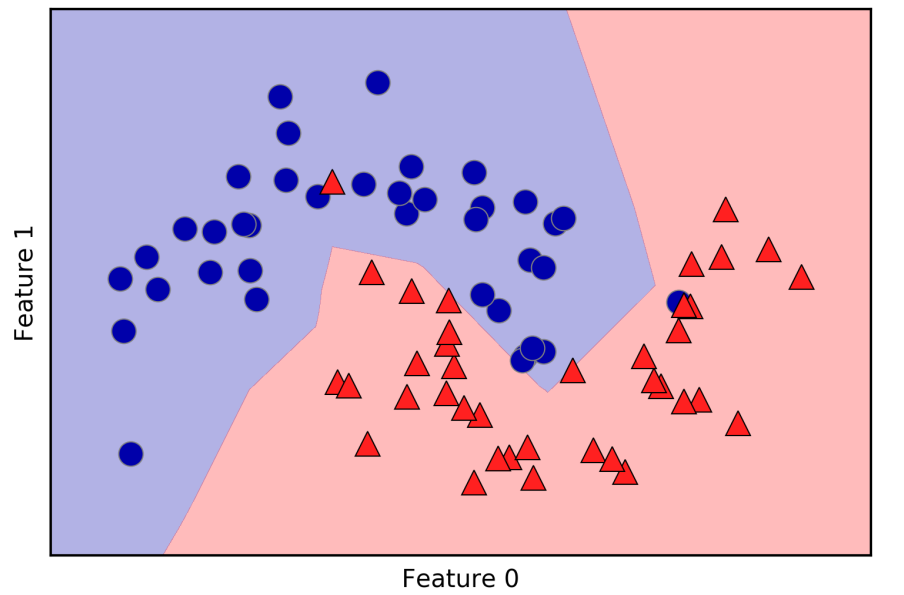
\includegraphics[scale=0.50]{../Imagen_Machine/2nodos}
	\caption{Límite de decisión aprendido con 2 capas ocultas con 10 unidades ocultas cada una, y con la activación de función de rectificación.}
	\label{2nodos}
\end{figure}

\begin{lstlisting}	

In[96]: # usando dos capas ocultas, con diez unidades cada una, ahora con 
        #  tanh (no lineal)       
        mlp = MLPClassifier(solve='lbfgs', activation='tanh',
                            random_state=0, hidden_layer_sizes=[10, 10])
        mlp.fit(X_train, y_train)
        mglearn.plots.plot_2d_separator(mlp, X_train, fill=True, alpha=.3)
        mglearn.discrete_scatter(X_train[:, 0], X_train[:, 1], y_train)
        plt.xlabel("Feature 0")
        plt.ylabel("Feature 1")

\end{lstlisting}

\begin{figure}[h!]
	\centering
	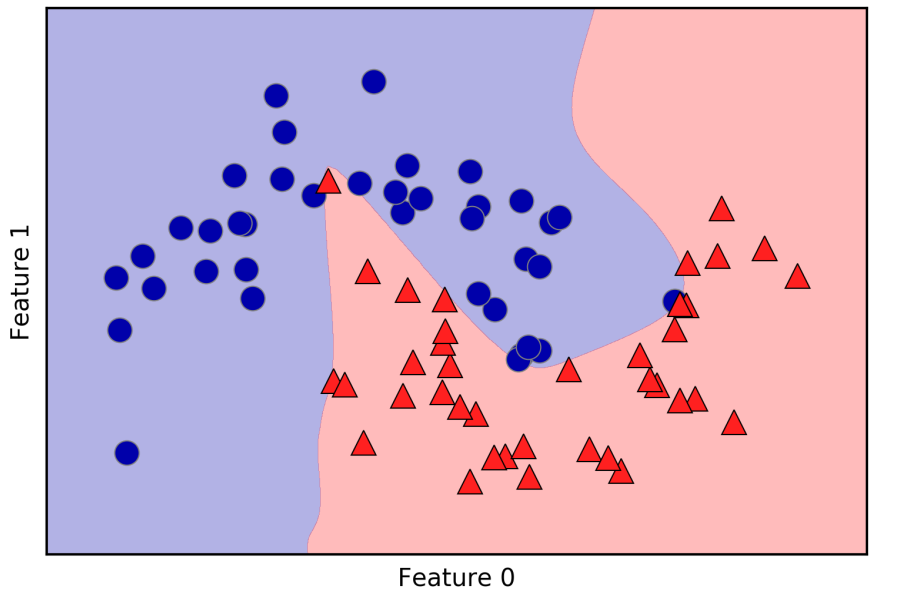
\includegraphics[scale=0.50]{../Imagen_Machine/2nodosTagh}
	\caption{Límite de decisión aprendido con 2 capas ocultas con 10 unidades ocultas cada una, con función de activación de tanh}
	\label{2nodosTagh}
\end{figure}

Por último, también podemos controlar la complejidad del modelo de  red neuronal  mediante el uso de una penalidad de tipo  $L2,$ para reducir los pesos hacia cero, como lo hicimos en la regresión Ridge y la clasificación lineal. El parámetro  del {\ttfamily Mlpclassifier} es  {\ttfamily alfa} (como en el modelo de regresión lineal),   por defecto está cofigurado con un valor muy bajo (poca regularización). La figura \ref{DiferenteHidden} muestra el efecto de diferentes valores de  {\ttfamily alfa} en el conjunto de datos {\ttfamily two\_moons}, utilizando dos capas ocultas de 10 o 100 unidades cada una:

\begin{lstlisting}  

In[97]: fig, axes = plt.subplots(2, 4, figsize=(20, 8))
        for axx, n_hidden_nodes in zip(axes, [10, 100]):
            for ax, alpha in zip(axx, [0.0001, 0.01, 0.1, 1]):
                 mlp = MLPClassifier(solve='lbfgs', random_state=0,
                                     hidden_layer_sizes=[n_hidden_nodes,
                                     n_hidden_nodes], alpha=alpha)
                 mlp.fit(X_train, y_train)
                 mglearn.plots.plot_2d_separator(mlp, X_train, fill=True, 
                                                 alpha=.3, ax=ax)
                 mglearn.discrete_scatter(X_train[:, 0], X_train[:, 1], 
                                          y_train, ax=ax)
                 ax.set_title("n_hidden=[{}, {}]\nalpha={:.4f}".format(
                               n_hidden_nodes, n_hidden_nodes, alpha))

\end{lstlisting}


\begin{figure}[h!]
	\centering
	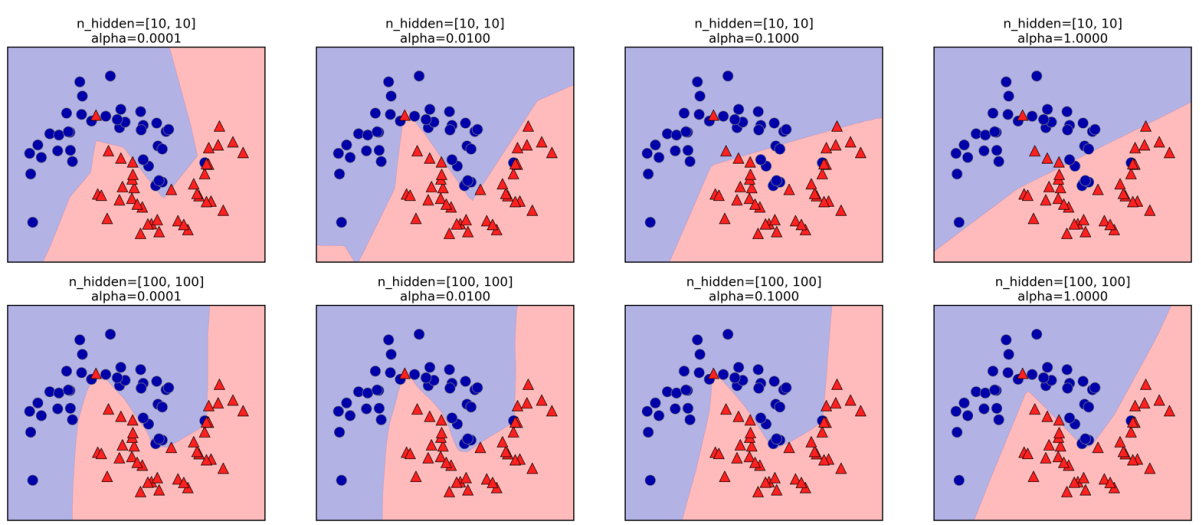
\includegraphics[scale=0.50]{../Imagen_Machine/DiferenteHidden}
	\caption{Funciones de decisión para diferentes números de unidades ocultas y diferentes ajustes del parámetro alfa }
	\label{DiferenteHidden}
\end{figure}


Hay muchas formas para controlar la complejidad de una red neuronal: mediante el número de capas ocultas, por el número de unidades en cada capa oculta, y la regularización {\ttfamily alfa}.  Realmente hay  más, pero no serán tratamos aquí. \\

Una propiedad importante en redes neuronales es que sus pesos están colocados al azar
antes comenzar  el aprendizaje, y esta  aleatoriedad inicial afecta el modelo  aprendido. Esto significa  que  aún cuando usen exactamente los mismos parámetros, se pueden  obtener modelos muy diferentes al usar  semillas diferentes. Si las redes son grandes, y su complejidad está seleccionada  correctamente, ésto no debería afectar mucho la exactitud, pero esto es importante tenerlo  pendiente (en particular para redes más pequeñas). La figura \ref{RandonDif}  muestra varios modelos, todos aprendiendo con la misma configuración  de parámetros (efecto de semilla aleatoria).


\begin{lstlisting}  % [frame=single]	

In[98]: fig, axes = plt.subplots(2, 4, figsize=(20, 8))
        for i, ax in enumerate(axes.ravel()):
            mlp = MLPClassifier(algorithm='l-bfgs', random_state=i,
                                 hidden_layer_sizes=[100, 100])
            mlp.fit(X_train, y_train)
            mglearn.plots.plot_2d_separator(mlp, X_train, fill=True,
                                            alpha=.3, ax=ax)
            mglearn.discrete_scatter(X_train[:, 0], X_train[:, 1], 
                                      y_train, ax=ax)

\end{lstlisting}


\begin{figure}[h!]
	\centering
	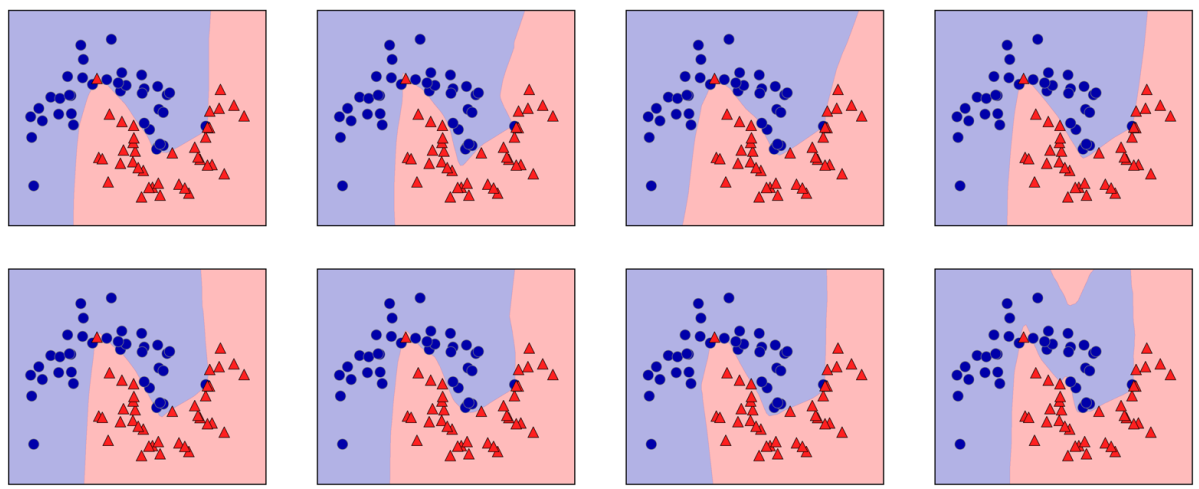
\includegraphics[scale=0.50]{../Imagen_Machine/RandonDif}
	\caption{Funciones de decisión aprendidas con los mismos parámetros, pero con diferente iniciación aleatorias}
	\label{RandonDif}
\end{figure}



Ahora apliquemos el  {\ttfamily  Mlpclassifier} a la dataset  cáncer de mama (Breast Cancer), para obtener una mejor comprensión de las redes neuronales en datos del mundo real. y comencemos  con los parámetros 
por defecto: \\

\begin{lstlisting}  % [frame=single]	

In[99]: print("Cancer data per-feature maxima:\n{}".format(
                cancer.data.max(axis=0)))

Out[99]:

    Cancer data per-feature maxima:
    [ 28.110   39.280   188.500  2501.000  0.163   0.345    0.427
       0.201    0.304     0.097     2.873  4.885  21.980  542.200
       0.031    0.135     0.396     0.053  0.079   0.030   36.040
      49.540  251.200  4254.000     0.223  1.058   1.252    0.291
       0.664    0.207]
      
In[100]:  X_train, X_test, y_train, y_test = train_test_split(
               cancer.data, cancer.target, random_state=0)
       
          mlp = MLPClassifier(random_state=42)
          mlp.fit(X_train, y_train)
   
          print("Accuracy on training set: {:.2f}".format(
                 mlp.score(X_train, y_train)))
          print("Accuracy on test set: {:.2f}".format(
                 mlp.score(X_test, y_test)))

Out[100]:
   
   Accuracy on training set: 0.92
   Accuracy on test set: 0.90


\end{lstlisting}


La exactitud  del MLP es muy  bueno, pero no tan bueno como los otros modelos. Así como en el anterior ejemplo de SVC, esto es probablemente debido a la escala de los datos. Las redes neuronales también esperan que todas las características de entradas  varien en forma similar, e idealmente que tengan media cero, y varianza uno.

 Así que debemos re-escalar los datos a fin de que cumpla con estos requisitos. En en próximo ejemplo, se hace el re-escalado de datos a mano, pero en el Capítulo \ref{Cap3} introduciremos  el  StandardScaler para hacerlo automáticamente:\\

\begin{lstlisting} 
In[101]: # compute the mean value per feature on the training set
         mean_on_train = X_train.mean(axis=0)
         # compute the standard deviation of each feature on the training set
         std_on_train = X_train.std(axis=0)
   
         # subtract the mean, and scale by inverse standard deviation
         # afterward, mean=0 and std=1
         X_train_scaled = (X_train - mean_on_train) / std_on_train
         # use THE SAME transformation (using training mean and std)
         # on the test set
         X_test_scaled = (X_test - mean_on_train) / std_on_train
   
         mlp = MLPClassifier(random_state=0)
         mlp.fit(X_train_scaled, y_train)
   
         print("Accuracy on training set: {:.3f}".format(
                mlp.score(X_train_scaled, y_train)))
         print("Accuracy on test set: {:.3f}".format(
                mlp.score(X_test_scaled, y_test)))
  
Out[101]:
   
    Accuracy on training set: 0.991
    Accuracy on test set: 0.965

    ConvergenceWarning:
        Stochastic Optimizer: Maximum iterations reached and the
        optimization hasn't converged yet.


\end{lstlisting}

Los resultados han mejorado mucho después de re-escalar, y bastante competitiva. Sin embargo, Tenemos un 
advertencia del modelo, que nos dice que el máximo número de iteraciones ha sido alcanzado. Esto es parte del algoritmo  {\ttfamily adam }  para el aprendizaje del modelo, y nos dice que deberíamos aumentar el número de iteraciones:


\begin{lstlisting}  

In[102]: mlp = MLPClassifier(max_iter=1000, random_state=0)
         mlp.fit(X_train_scaled, y_train)

         print("Accuracy on training set: {:.3f}".format(
                mlp.score(X_train_scaled, y_train)))
         print("Accuracy on test set: {:.3f}".format(
	            mlp.score(X_test_scaled, y_test)))

Out[102]:

    Accuracy on training set: 0.995
    Accuracy on test set: 0.965
\end{lstlisting}


El incremento del número de iteraciones, sólo aumentó el rendimiento del conjunto de entrenamiento, y no
el rendimiento de generalización. Pero todavía, el modelo tiene un rendimiento bastante bueno.  Como hay 
alguna diferencia  entre el rendimiento en el conjunto de  entrenamiento y  prueba, podríamos intentar bajar la complejidad del modelo, para tener mejor rendimiento de generalización. Aquí, elegimos
aumentar el parámetro {\ttfamily alfa} (muy agresivamente, de  0.0001 al 1), para añadir una regularización más fuerte  a los pesos:


\begin{lstlisting}  

In[103]: mlp = MLPClassifier(max_iter=1000, alpha=1, random_state=0)
         mlp.fit(X_train_scaled, y_train)
   
         print("Accuracy on training set: {:.3f}".format(
                 mlp.score(X_train_scaled, y_train)))
         print("Accuracy on test set: {:.3f}".format(
                 mlp.score(X_test_scaled, y_test)))

Out[103]:
     
     Accuracy on training set: 0.988
     Accuracy on test set: 0.972


\end{lstlisting}

Esto conduce a un rendimiento a la par con los mejores modelos hasta ahora{\footnote{\scriptsize{Usted puede haber notado en este punto que muchos de los modelos de buen desempeño alcanzaron exactamente la misma exactitud de 0.972. Esto significa que todos los modelos cometen exactamente el mismo número de errores, que son cuatro. ¡Si comparas las predicciones reales, puedes incluso ver que cometen exactamente los mismos errores! Esto podría ser una consecuencia de que el conjunto de datos sea muy pequeño, o puede ser porque estos puntos son realmente diferentes del resto}}}. \\

Si bien es posible analizar lo que una red neuronal ha aprendido, esto suele ser mucho más complicado que analizar un modelo lineal o un modelo basado en árboles. Una forma de 
analizar lo que fue aprendido por el modelo  es observar los pesos en el modelo.   Puede ver un ejemplo de esto en la  \href{http://scikit-learn.org/stable/auto_examples/neural_networks/plot_mnist_filters.html}{\color{vino}      galería de ejemplo de scikit-learn}.  Para la  dataset de cáncer de mama, esto podría sea un poco difícil de entender. El siguiente gráfico  (figura \ref{ponderaciones}) muestra los pesos que se aprendieron conectando la entrada a la primera capa oculta. Las filas de este gráfico corresponde a las 30 características de entrada,  mientras las columnas  corresponden a las 100 unidades ocultas. Los colores claros representan valores positivos grandes, mientras los colores oscuros representan 
los valores negativos:\\

\begin{lstlisting}  % [frame=single]	

In[104]: plt.figure(figsize=(20, 5))
         plt.imshow(mlp.coefs_[0], interpolation='none', cmap='viridis')
         plt.yticks(range(30), cancer.feature_names)
         plt.xlabel("Columns in weight matrix")
         plt.ylabel("Input feature")
         plt.colorbar()

\end{lstlisting}


\begin{figure}[h!]
	\centering
	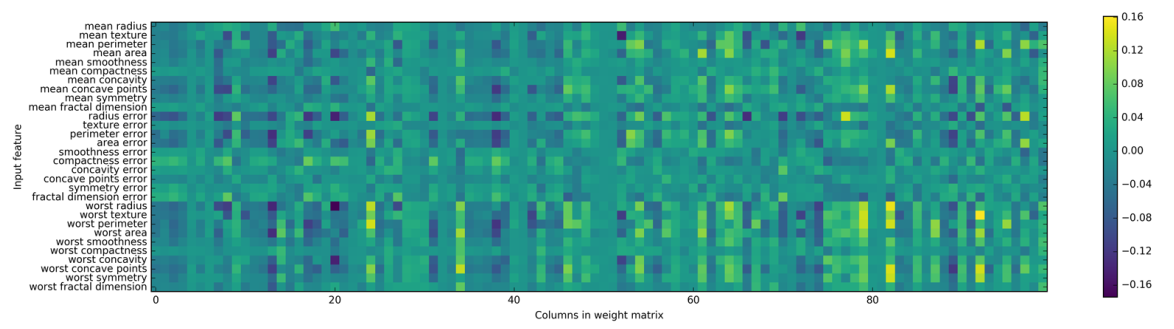
\includegraphics[scale=0.50]{../Imagen_Machine/ponderaciones}
	\caption{Mapa caliente de los pesos de la primera capa en una red neuronal aprendida en la dataset de Cáncer de Mama}
	\label{ponderaciones}
\end{figure}


Una posible inferencia que podemos hacer es que las características que tienen pesos muy pequeños para
todas las unidades ocultas son "menos importantes"{}   para el modelo. Podemos ver que   "{}mean smoothness"{}   y   "{}mean compactness"{},  además de las características encontradas entre  "{}smoothness error"{}  y  "{}fractal dimension error"{},  tienen pesos relativamente bajos en comparación con otras características. Esto podría significar que estas son características  son menos importantes  o posiblemente que no los representamos de una manera que la red neuronal podría utilizar.\\

También podríamos visualizar los pesos que conectan la capa oculta a la capa de salida, pero son aún más difíciles de interpretar.   Mientras que {\ttfamily MLPClassifier} y {\ttfamily MLPRegressor} proporcionan interfaces fáciles de usar para arquitecturas de redes neuronales más comunes, solo capturan un pequeño subconjunto de lo que es posible con redes neuronales.  Si estás interesado en trabajar con más flexibilidad
o modelos más grandes, te recomendamos que mires más allá de {\ttfamily scikit-learn,} aprende lo fantástico
 de las  librerías de  deep learning  (librerías de aprendizaje profundo) que están ahí libres. 

Para los usuarios de Python, lo  mejores librerías bien  establecidas son: {\ttfamily keras, lasagna},  y  {\ttfamily tensor-flow.  lasagna} se basa en la librería de {\ttfamily theano}, mientras {\ttfamily Keras} puede usar {\ttfamily tensor-flow  o  theano}.  Estas librerías proporcionan una interfaz mucho más flexible para construir redes neuronales y seguir el rápido progreso en la investigación del aprendizaje profundo. Todas las librerías más  populares de aprendizaje profundo también permiten el uso de unidades de procesamiento gráfico de alto rendimiento (graphics processing units  GPUs), que {\ttfamily scikit-learn} no soporta.  El uso de GPUs nos permite acelerar los cálculos por factores de 10x a 100x, y son esenciales para aplicar métodos de aprendizaje profundo en conjuntos de datos de gran escala.


\subsubsection{Fortalezas, debilidades y parámetros}



Las redes neuronales han resurgido como modelos de  última generación (vanguardia) en muchas 
aplicaciones de aprendizaje automático (machine learning). Una de sus principales ventajas es que pueden capturar información contenida en grandes cantidades de datos y construir modelos increíblemente complejos.
Dando suficiente tiempo de cálculo, datos y ajuste cuidadoso de los parámetros, las redes neuronales generalmente superan  otros algoritmos de aprendizaje automático (para tareas de clasificación y regresión).\\


Por otro lado, esto presenta algunos  inconvenientes o desventajas.
Las redes neuronales, particularmente las grandes y poderosas, a menudo tardan mucho tiempo en entrenarse, además requieren  de un  procesamiento previo a la data  muy cuidadoso, como hemos visto aquí.

De manera similar a los SVMs, funcionan mejor con data  "{}homogénea{},"{ }  donde todas las características tengan significados similares.  Para datos con  características muy diferentes, los modelos basados en árboles podrían funcionar mejor.  En nuestros experimentos, apenas descubrimos la cara sur de posibles formas de ajustar modelos de redes neuronales y cómo entrenarlos.   Configurar los parámetros de una red neuronal también es un arte en sí mismo. En los ejemplos tratados aquí,  apenas introducimos una pequeña parte de las formas posibles  de ajustar  modelos de redes neuronales y cómo entrenarlos.\\


\subsubsection{Estimación de la complejidad en las redes neuronales}

Los parámetros más importantes son el número de capas y el número de unidades ocultas por capa. Debe comenzar con una o dos capas ocultas, y posiblemente expandirse desde allí.  El número de nodos por capa oculta es a menudo similar al número de características de entrada, pero rara vez más alto que en el punto  medio  para  miles.\\

Una medida útil cuando se piensa en la complejidad del modelo de una red neuronal es el número de pesos o coeficientes que aprenden.  Si tiene una  dataset con  100 características para desarrollar una clasificación  binaria, y tiene 100 unidades ocultas, entonces hay 100 *100 = 10.000 pesos entre la entrada y la primera capa oculta. También hay 100 * 1 = 100  pesos entre la capa oculta y la capa de salida, para un total de alrededor de 10.100 pesos. Si agrega una segunda capa oculta con 100 unidades ocultas, allí
habrá otros 100 * 100 = 10.000 pesos de la primera capa oculta hasta la segunda
capa oculta, lo que resulta en un total de 20.100 pesos. 

Si en lugar de eso usas una capa con 1.000 unidades ocultas, tendras   100 * 1.000 = 100.000 pesos  aprendiendo  de la entrada hasta la capa oculta y los pesos de 1000 x 1 de  la capa oculta hasta la capa de salida, para un total de 101.000.  Si añade una segunda capa oculta, entonces se agregan  1.000 * 1.000 = 1.000.000  pesos, para un total  de 1.101.000; este modelo resulta  50 veces más grande que el modelo construido con dos capas ocultas de tamaño 100.\\

Una forma común de ajustar los parámetros en una red neuronal es crear primero una red
 suficientemente grande que genere  sobreajuste en el modelo, claro aquí asegura que la tarea pueda 
ser realmente aprendida por la red, y luego, sabiendo que  los datos de entrenamiento  pueden aprender, se reduce la red o se aumenta el parámetro  {\ttfamily alfa} para añadir regularización, que mejorará el rendimiento de generalización.\\

En estos ejemplos nos enfocamos más en la definición del modelo: el número de
capas y nodos por capa, la regularización y la no linealidad. Estos parámetros  definen el
modelo que queremos aprender. También está la cuestión de cómo aprende el modelo, o  
el algoritmo que se usa para el aprendizaje de los parámetros, el cual es configurado por los parámetro del algoritmo.

El algoritmo  tiene dos opciones fáciles de usar: Uno es el {\ttfamily "adam"{}},  que es el valor por defecto,  este funciona bien en la mayoría de las situaciones, pero es muy  sensible a la escala de los datos (por lo que es importante siempre re-escalar los datos a 0 media y varianza 1).   El otro es {\ttfamily "{}l-bfgs"{}},  el cual es bastante robusto pero puede hacer  un tiempo largo en modelos grandes o dataset  grandes. También está la opción más avanzada  {\ttfamily  "{}sgd"{}},  que es lo que muchos  investigadores del aprendizaje profundo emplean. La opción   {\ttfamily "{}sgd"{}}  viene con muchos parámetros adicionales, que necesitan ser  ajustados  para obtener mejores resultados.  Puede encontrar todos estos parámetros y  sus definiciones en la guía del usuario.  Al comenzar a trabajar con MLPs, le recomendamos  apegarse a {\ttfamily "adam"{}} y {\ttfamily "{}l-bfgs"{}}.\\


\begin{minipage}[t]{0.2\textwidth}
	\centering\raisebox{\dimexpr \topskip-\height}{%
		
\includegraphics[width=\textwidth]{Imagen_Machine/Pajaro.png}}
\end{minipage}%\hfill
\begin{minipage}[t]{0.75\textwidth} 
	{\scriptsize	
	{\bf{fit restablece un modelo (fit Resets a Model)}:}
		
		Una propiedad importante de los modelos de {\ttfamily scikit-learn} es que llamando {\ttfamily fit} siempre restablecerá todo lo que un modelo previamente ha aprendido.   Así que si construye un modelo en un conjunto de datos, y luego llama {\ttfamily fit} de nuevo sobre un conjunto de datos diferente, el modelo "{}olvidará"{}  todo lo que aprendió del primer conjunto de datos. Puede llamar a {\ttfamily fit} tanto  como desee en un modelo, y el resultado será el mismo que llamar {\ttfamily fit} en un "{}nuevo"{}  modelo.}
\end{minipage}

\subsubsection{Estimaciones de incertidumbre de los clasificadores}


Un tema importante y muy útil  del que aún no hemos hablado  en la interfaz de {\ttfamily scikit-learn}, es
la capacidad de los clasificadores de proveer estimaciones de incertidumbre de las predicciones.  A menudo estamos interesados no sólo  en la  clase que predice un clasificador para un cierto punto de prueba, sino también que tan seguro estamos de que la clase es la correcta. En la práctica, diferentes tipos de errores conducen a resultados muy diferentes en aplicaciones del mundo real. Imaginemos  una aplicación médica sobre pruebas sobre una enfermedad, por ejemplo el cáncer.  Hacer una predicción falsa positiva puede llevar a que el paciente se someta a  pruebas adicionales; mientras que una predicción falsa negativa puede llevar al paciente a consecuencias graves al no tratar la enfermedad a tiempo.  Este tema lo  trataremos  con mayor detalle en el Capítulo \ref{Cap6}.\\

 

Hay dos funciones en {\ttfamily scikit-learn} que se pueden utilizar para 
obtener estimaciones de la incertidumbre de los clasificadores, estas son:   {\ttfamily predict\_proba} y  {\ttfamily decision\_function}.   La  mayoría (pero no todos)  de los clasificadores tienen al menos uno de ellos, y muchos clasificadores tienen ambos. \\ 

Analicemos  lo que hacen estas dos funciones sobre la  dataset bidimensional sintético,  cuando se emplea 
 el  clasificador {\ttfamily GradientBoostingClassifier}, que tiene ambas funciones,  la  {\ttfamily decision\_function}  y la  {\ttfamily predict\_proba}:\\


\begin{lstlisting}  % [frame=single]	

In[105]: from sklearn.ensemble import GradientBoostingClassifier
         from sklearn.datasets import make_blobs, make_circles
         X, y = make_circles(noise=0.25, factor=0.5, random_state=1)
   
         # we rename the classes "blue" and "red" for illustration 
         # purposes
         y_named = np.array(["blue", "red"])[y]
   
        # we can call train_test_split with arbitrarily many arrays;
        # all will be split in a consistent manner
        X_train, X_test, y_train_named, y_test_named, y_train, y_test = \
             train_test_split(X, y_named, y, random_state=0)
   
        # build the gradient boosting model
        gbrt = GradientBoostingClassifier(random_state=0)
        gbrt.fit(X_train, y_train_named)


\end{lstlisting} 




\subsubsection*{La función de decisión}

En el caso de clasificación binaria, el valor de retorno de la función\index{función de decisión}   {\ttfamily decision\_function} tiene forma {\ttfamily (n\_samples,)}, y devuelve un número de punto flotante para cada muestra:\\

\begin{lstlisting}  % [frame=single]	

In[106]: print("X_test.shape: {}".format(X_test.shape))
         print("Decision function shape: {}".format(
                gbrt.decision_function(X_test).shape))

Out[106]:

    X_test.shape: (25, 2)
    Decision function shape: (25,)

\end{lstlisting} 


Este valor codifica con qué rigor  el modelo afirma  que un  dato pertenece a la
clase "positiva", en este caso clase 1. Los valores positivos indican una preferencia por la 
clase positiva, y los valores negativos indican una preferencia por la clase "negativa"{ }:\\

\begin{lstlisting}  % [frame=single]	

In[107]: # show the first few entries of decision_function
         print("Decision function:\n{}".format(
                 gbrt.decision_function(X_test)[:6]))
 
Out[107]:

    Decision function:
    [ 4.136 -1.683 -3.951 -3.626 4.29 3.662]
    
\end{lstlisting}


\noindent Podemos recuperar la predicción  sólo observando el signo de la función de decisión:\\
 
	\begin{lstlisting}  % [frame=single]	

In[108]: print("Thresholded decision function:\n{}".format(
         gbrt.decision_function(X_test) > 0))
         print("Predictions:\n{}".format(gbrt.predict(X_test)))

Out[108]:

    Thresholded decision function:
    [ True False False False True True False True True True False True
      True False True False False False True True True True True False
      False]

    Predictions:
    ['red' 'blue' 'blue' 'blue' 'red' 'red' 'blue' 'red' 'red' 'red' 'blue'
     'red' 'red' 'blue' 'red' 'blue' 'blue' 'blue' 'red' 'red' 'red' 'red'
     'red' 'blue' 'blue']

\end{lstlisting} 


Para la clasificación binaria, la clase "negativa"{ }   es siempre la primera entrada del atributo {\ttfamily clases\_}, y la clase "positiva"{ }  es la segunda entrada. Entonces si quieres recuperar completamente la salida de predicción, debe hacer uso del atributo {\ttfamily classes\_}:\\

	\begin{lstlisting}  % [frame=single]	

In[109]: # make the boolean True/False into 0 and 1
         greater_zero = (gbrt.decision_function(X_test) > 0).astype(int)
         # use 0 and 1 as indices into classes_
         pred = gbrt.classes_[greater_zero]
         # pred is the same as the output of gbrt.predict
         print("pred is equal to predictions: {}".format(
                np.all(pred == gbrt.predict(X_test))))

Out[109]:

    pred is equal to predictions: True
\end{lstlisting}

El rango de {\ttfamily decision\_function} puede ser arbitrario, y depende de los datos y los parámetros del modelo:


\begin{lstlisting}  % [frame=single]	

In[110]: decision_function = gbrt.decision_function(X_test)
         print("Decision function minimum: {:.2f} maximum: {:.2f}".format(
                np.min(decision_function), np.max(decision_function)))

Out[110]:

    Decision function minimum: -7.69 maximum: 4.29

\end{lstlisting}

Este escalado arbitrario hace que la salida de {\ttfamily decision\_function} sea un poco difícil para interpretar.\\

En el ejemplo siguiente graficamos  la función {\ttfamily decision\_function} para todos los puntos en el plano 2D, usando una codificación de color  junto a al límite de decisión, como vimos anteriormente. Los  datos  de entrenamiento se presentan como círculos y  de  prueba como  triángulos (Figure \ref{Toy2}):\\

\begin{lstlisting} 

In[111]: fig, axes = plt.subplots(1, 2, figsize=(13, 5))
         mglearn.tools.plot_2d_separator(gbrt, X, 
                                         ax=axes[0], alpha=.4,
                                         fill=True, cm=mglearn.cm2)
         scores_image = mglearn.tools.plot_2d_scores(gbrt, X,
                                                     ax=axes[1],
                                                     alpha=.4, 
                                                     cm=mglearn.ReBl)
                                               
          for ax in axes:
              # plot training and test points
              mglearn.discrete_scatter(X_test[:, 0], X_test[:, 1], 
                                       y_test, markers='^', ax=ax)
              mglearn.discrete_scatter(X_train[:, 0], X_train[:, 1],
                                        y_train, markers='o', ax=ax)
              ax.set_xlabel("Feature 0")
              ax.set_ylabel("Feature 1")
          cbar = plt.colorbar(scores_image, ax=axes.tolist())
          axes[0].legend(["Test class 0", "Test class 1", 
                           "Train class 0","Train class 1"],
                            ncol=4, loc=(.1, 1.1))

\end{lstlisting}



\begin{figure}[h!]
	\centering
	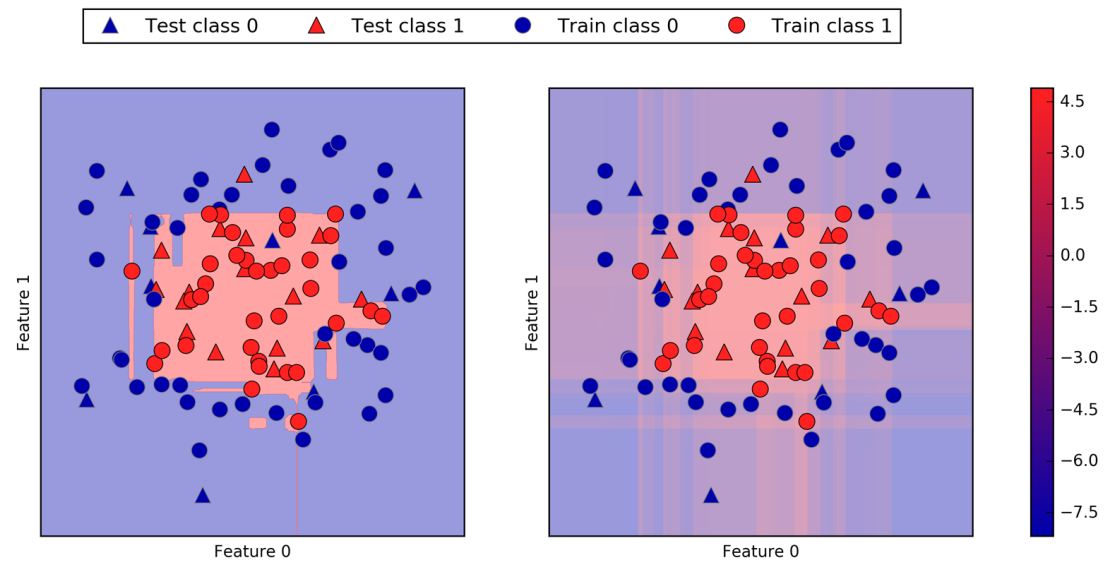
\includegraphics[scale=0.50]{../Imagen_Machine/Toy2}
	\caption{Límite de decisión (izquierda) y función de decisión (derecha) para un modelo de gradient boosting en la dataset de Toy bidimensional.}
	\label{Toy2}
\end{figure}

Codificar no solo el resultado predicho sino también la certeza del clasificador proporciona información adicional. Sin embargo, en esta visualización, es difícil distinguir el límite entre las dos clases.



\subsubsection{Probabilidades de predicción}


La salida de {\ttfamily predic\_proba} es una probabilidad\index{probabilidades de predicción} para cada clase, y  generalmente es más fácil
de entender  que la salida de {\ttfamily decision\_function}. Éste siempre tiene la forma de {\ttfamily (n\_samples, 2)} para clasificación binaria:\\

\begin{lstlisting}

In[112]: print("Shape of probabilities: {}".format(
                 gbrt.predict\_proba(X\_test).shape))

Out[112]:

   Shape of probabilities: (25, 2)

\end{lstlisting}


La primera entrada en cada fila es la probabilidad estimada de la primera clase, y la segunda
 entrada es la probabilidad estimada de la segunda clase. Debido a que es una probabilidad,
la salida de {\ttfamily predic\_proba} siempre está entre 0 y 1, y la suma de las entradas
para ambas clases es siempre 1:\\

\begin{lstlisting}

In[113]: # show the first few entries of predict_proba
         print("Predicted probabilities:\n{}".format(
                gbrt.predict_proba(X_test[:6])))


Out[113]:

   Predicted probabilities:
   [[ 0.016 0.984]
    [ 0.843 0.157]
    [ 0.981 0.019]
    [ 0.974 0.026]
    [ 0.014 0.986]
    [ 0.025 0.975]]
    

\end{lstlisting} 



Debido a que las probabilidades para las dos clases suman 1, exactamente una de las dos  clases
debería estar por encima del 50\% de certeza. Esa clase es la que se predice (las probabilidades son números flotante, puede suceder aunque es poco probable que ambos sean exactamente 0.500; sin embargo, si es el caso, la predicción se hace al azar). Puedes ver en el resultado anterior que el clasificador es relativamente seguro para la mayoría puntos. El grado de incertidumbre reflejada  realmente  depende del modelo y de los parámetros.   Un modelo con  mayor  sobreajuste tiende a hacer predicciones más seguras, incluso si podrían estar erradas. Un modelo con menos complejidad generalmente tiene más   incertidumbre en sus predicciones.    Un modelo se llama calibrado\index{modelo calibrado } si la incertidumbre reporta  realmente  las coincidencias  con lo correcto: esto es en un modelo calibrado, un una predición  hecha con un 70\% de certeza sería correcta el 70\% de las veces.\\ 
 

En el siguiente ejemplo (Figura \ref{Toy3} ) nuevamente mostramos el límite de decisión en el
conjunto de datos, junto a las probabilidades de clase para la clase 1:\\


\begin{lstlisting}  % [frame=single]	

In[114]: fig, axes = plt.subplots(1, 2, figsize=(13, 5))
   
         mglearn.tools.plot_2d_separator(gbrt, X, ax=axes[0], 
                                         alpha=.4, fill=True, 
                                         cm=mglearn.cm2)
         scores_image = mglearn.tools.plot_2d_scores(gbrt, X, ax=axes[1], 
                                                     alpha=.5, cm=mglearn.ReBl,
                                                     function='predict_proba')
       
         for ax in axes:
             # plot training and test points
             mglearn.discrete_scatter(X_test[:, 0], X_test[:, 1],
                                      y_test, markers='^', ax=ax)
             mglearn.discrete_scatter(X_train[:, 0], X_train[:, 1], 
                                      y_train, markers='o', ax=ax)
             ax.set_xlabel("Feature 0")
             ax.set_ylabel("Feature 1")
      cbar = plt.colorbar(scores_image, ax=axes.tolist())
      axes[0].legend(["Test class 0", "Test class 1", "Train class 0",
                      "Train class 1"], ncol=4, loc=(.1, 1.1))

\end{lstlisting} 


\begin{figure}[h!]
	\centering
	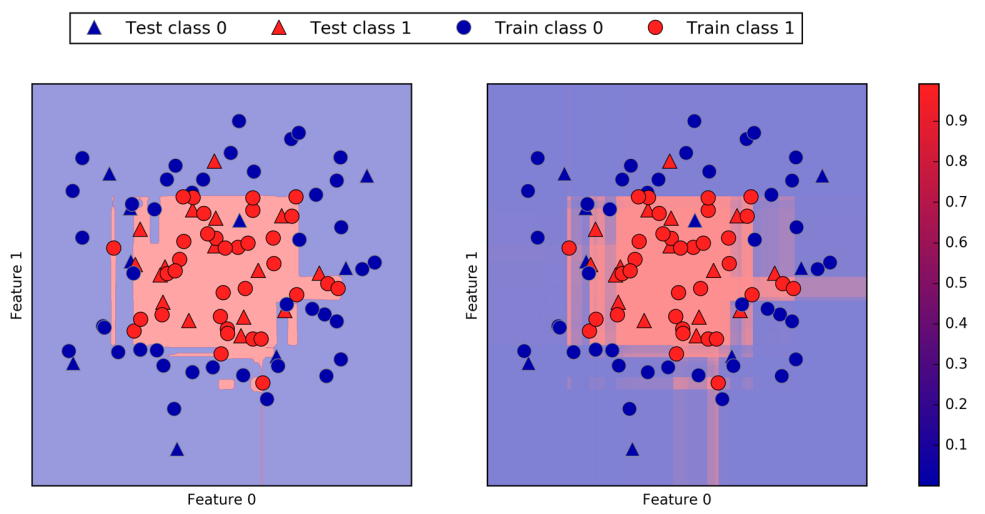
\includegraphics[scale=0.50]{../Imagen_Machine/Toy3}
	\caption{Límite de decisión (izquierda) y predición de probabilidades para el modelo gradient 
		boosting mostrado en la Figura \ref{Toy2}}
	\label{Toy3}
\end{figure}





 Los límites en este gráfico están mucho más bien definidos, y las pequeñas áreas de incertidumbre son claramente visibles.\\
 
  El \href{http://bit.ly/2cqCYx6}{\color{vino} sitio web de {\ttfamily scikit-learn}}  tiene una gran comparación de muchos modelos y cómo se ven sus estimaciones de incertidumbre. Hemos reproducido esto en la Figura \ref{Incerti}, y le recomendamos seguir a través del ejemplo.

\begin{figure}[h!]
	\centering
	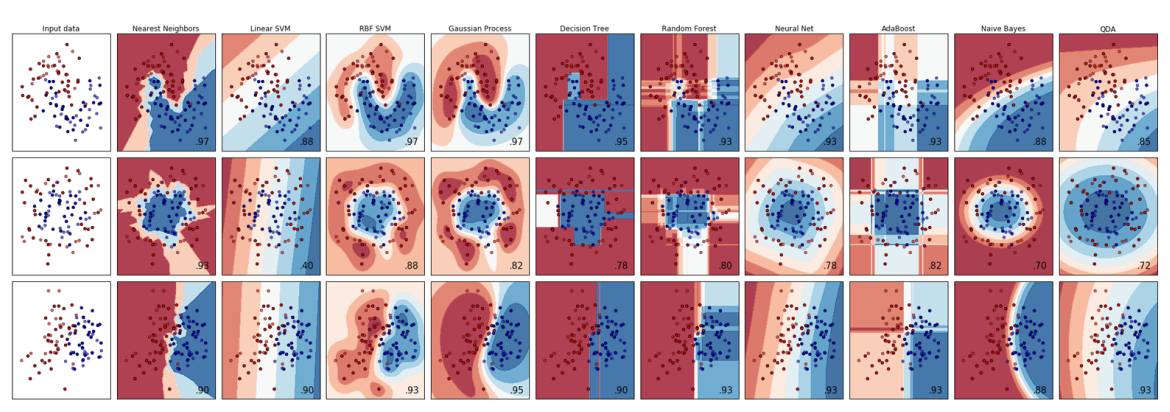
\includegraphics[scale=0.55]{../Imagen_Machine/Incerti}
	\caption{Comparación de varios clasificadores en scikit-learn sobre la data de sintéticos (imagen cortesía de  \href{http://scikit-learn.org\%29/}{\color{vino} http://scikit-learn.org})}
	\label{Incerti}
\end{figure}


\subsubsection*{Incertidumbre en la clasificación multiclase}

Hasta ahora, sólo hemos hablado de estimaciones de incertidumbre en la clasificación binaria. Pero los métodos {\ttfamily decision\_function}  y  {\ttfamily predict\_proba}  también funcionan en el entorno multiclase. \\

Ilustremos con la data  Iris, que es una data  de clasificación en tres clases:



\begin{lstlisting}  % [frame=single]	


In[115]: from sklearn.datasets import load_iris
   
         iris = load_iris()
         X_train, X_test, y_train, y_test = train_test_split(
               iris.data, iris.target, random_state=42)
       
         gbrt = GradientBoostingClassifier(learning_rate=0.01,
                                            random_state=0)
         gbrt.fit(X_train, y_train)
   
In[116]: print("Decision function shape: {}".format(
                gbrt.decision_function(X_test).shape))
         # plot the first few entries of the decision function
         print("Decision function:\n{}".format(
                 gbrt.decision_function(X_test)[:6, :]))
 
Out[116]:
    
    Decision function shape: (38, 3)
    Decision function:
    [[-0.529 1.466 -0.504]
     [ 1.512 -0.496 -0.503]
     [-0.524 -0.468 1.52 ]
     [-0.529 1.466 -0.504]
     [-0.531 1.282 0.215]
     [ 1.512 -0.496 -0.503]]

\end{lstlisting} 


En el caso multiclase, la {\ttfamily decision\_function}  tiene la forma {\ttfamily  (n\_samples, n\_classes)} y cada columna proporciona una "{}puntuación de certeza"{ }  para cada clase, donde una gran puntuación  significa que una clase es más probable y una puntuación pequeña significa que la clase es menos probable. Usted puede recuperar las predicciones de estas puntuaciones mediante la búsqueda de la entrada máxima para cada punto de datos:\\


\begin{lstlisting}  % [frame=single]	

In[117]: print("Argmax of decision function:\n{}".format(
                np.argmax(gbrt.decision_function(X_test), axis=1)))
         print("Predictions:\n{}".format(gbrt.predict(X_test)))

Out[117]:
   
    Argmax of decision function:
    [1 0 2 1 1 0 1 2 1 1 2 0 0 0 0 1 2 1 1 2 0 2 0 2 2 2 2 2 0 0 0 0 1 0 0 2 1 0]
    Predictions:
    [1 0 2 1 1 0 1 2 1 1 2 0 0 0 0 1 2 1 1 2 0 2 0 2 2 2 2 2 0 0 0 0 1 0 0 2 1 0]


\end{lstlisting} 


La salida de {\ttfamily predict\_proba} tiene la misma forma, {\ttfamily(n\_samples, n\_classes)}. Una vez más, las probabilidades de las clases posibles para cada punto de datos suma a 1:



\begin{lstlisting}  % [frame=single]	

In[118]: # show the first few entries of predict_proba
         print("Predicted probabilities:\n{}".format(
                  gbrt.predict_proba(X_test)[:6]))
         # show that sums across rows are one
         print("Sums: {}".format(
                 gbrt.predict_proba(X_test)[:6].sum(axis=1)))

Out[118]:

    Predicted probabilities:
    [[ 0.107 0.784 0.109]
     [ 0.789 0.106 0.105]
     [ 0.102 0.108 0.789]
     [ 0.107 0.784 0.109]
     [ 0.108 0.663 0.228]
     [ 0.789 0.106 0.105]]
Sums: [ 1. 1. 1. 1. 1. 1.]

\end{lstlisting} 

Podemos recuperar de nuevo las predicciones mediante el cálculo del {\ttfamily argmax}  de {\ttfamily predict\_proba}:


\begin{lstlisting}  % [frame=single]	


In[119]: print("Argmax of predicted probabilities:\n{}".format(
         np.argmax(gbrt.predict_proba(X_test), axis=1)))
         print("Predictions:\n{}".format(gbrt.predict(X_test)))

Out[119]:
   
    Argmax of predicted probabilities:
    [1 0 2 1 1 0 1 2 1 1 2 0 0 0 0 1 2 1 1 2 0 2 0 2 2 2 2 2 0 0 0 0 1 0 
     0 2 1 0]
    Predictions:
    [1 0 2 1 1 0 1 2 1 1 2 0 0 0 0 1 2 1 1 2 0 2 0 2 2 2 2 2 0 0 0 0 1 0 
     0 2 1 0]

\end{lstlisting} 


Para resumir, la función {\ttfamily predict\_proba}  y  {\ttfamily\_function} siempre tienen forma {\ttfamily (n\_sam ples, n\_classes)}, aparte de {\ttfamily decision\_function} en el caso especial  binario, {\ttfamily decision\_function} sólo tiene una columna, que corresponde a la clase  "positive"{}    
{\ttfamily classes\_[1] }. Esto es principalmente por razones históricas.\\

 Se puede recuperar la predicción cuando hay {\ttfamily n\_classes} (muchas columnas) mediante el cálculo del {\ttfamily argmax} a través de las columnas. Sin embargo, tenga cuidado, si sus clases son strings (cadenas de texto), o usa números enteros, pero no son consecutivos y a partir de 0. Si desea comparar los resultados obtenidos con el predict con los resultados obtenidos a través de {\ttfamily decision\_function} o pre {\ttfamily dict\_proba}, asegúrese de usar el atributo {\ttfamily classes\_} del clasificador para obtener los nombres de clase reales:


\begin{lstlisting}  % [frame=single]	

In[120]: logreg = LogisticRegression()
         # represent each target by its class name in the iris dataset
         named_target = iris.target_names[y_train]
         logreg.fit(X_train, named_target)
         print("unique classes in training data: {}".format(
                logreg.classes_))
         print("predictions: {}".format(logreg.predict(X_test)[:10]))
         argmax_dec_func = np.argmax(logreg.decision_function
                                     X_test), axis=1)
         print("argmax of decision function: {}".format(
                argmax_dec_func[:10]))
         print("argmax combined with classes_: {}".format(
                logreg.classes_[argmax_dec_func][:10]))
   
Out[120]:

    unique classes in training data: ['setosa' 'versicolor' 'virginica']
    predictions: ['versicolor' 'setosa' 'virginica' 'versicolor' 
     'versicolor' 'setosa' 'versicolor' 'virginica' 'versicolor'
     'versicolor']
    argmax of decision function: [1 0 2 1 1 0 1 2 1 1]
    argmax combined with classes_: ['versicolor' 'setosa' 'virginica' 
     'versicolor' 'versicolor' 'setosa' 'versicolor' 'virginica' 'versicolor'
     'versicolor']

\end{lstlisting} 



\subsubsection{Resumen y perspectivas}\ref{Pagina127} 

Comenzamos este capítulo con una discusión sobre la complejidad del modelo, luego discutimos 
generalización, o aprendizaje de un modelo que puede rendir (desenpeño) bien con datos nuevos, nunca antes vistos. Esto nos llevó a los conceptos de falta de ajuste, que describe un modelo que no puede
capturar las variaciones presentes de los datos de entrenamiento,  y el sobreajuste que describe un
modelo que se enfoca demasiado en los datos de entrenamiento y no puede generalizar bien con datos nuevos.

Luego discutimos una amplia gama de modelos de aprendizaje automático (machine learning) para la clasificación y regresión, con sus ventajas y desventajas, y cómo controlar 
complejidad  del modelo para cada uno de ellos.  Vimos que para muchos de los algoritmos, configurar los  parámetros correctos  es muy importante para un buen rendimiento.   Algunos de los algoritmos también son sensibles a cómo representamos los datos de entrada, y en particular a la escala de las características. Por lo tanto, aplicar a ciegas  un algoritmo a un conjunto de datos sin comprender los supuestos que hace el modelo y los significados de la configuración de los parámetros rara vez conducen a un modelo exacto.\\


Este capítulo contiene mucha información sobre los algoritmos, y no es necesario que recuerdes todos estos detalles para los capítulos.  Sin embargo, algún conocimiento de los modelos descritos aquí, y cuáles usar en una situación específica es importante para aplicar con éxito el aprendizaje automático en la práctica. Aquí hay un resumen rápido de cuándo usar cada modelo\index{cuando usar el modelo}:\\



{\bf Vecinos más cercanos }

Para dataset pequeños, buenos como línea de base, fáciles de explicar.\\

{\bf Modelos lineales}

Va  como un primer algoritmo para probar, bueno para conjuntos de datos muy grandes,  y para datos de muy alta dimensión.\\


{\bf Naives Bayes}

 Solo para clasificación. Incluso más rápido que los modelos lineales, bueno para datos muy grandes.
conjuntos y datos de alta dimensión. A menudo menos exacto que los modelos lineales.\\


{ \bf Árboles de decisión}

Muy rápido, no necesita escalar los datos, puede visualizarse y explicarse fácilmente.\\

{\bf Bosques aleatorios}

Casi siempre se desempeña mejor que un solo árbol de decisión, muy robusto y potente. No es necesario escalar los datos. No es bueno para data sparse de muy alta dimensión.\\


{\bf Gradiente potenciado}

A menudo un poco más exacto  que los bosques aleatorios. Más lento para entrenar pero más rápido para
predecir que los bosques aleatorios, y menos  memoria. Necesita más ajuste de parámetros
 que bosques aleatorios.\\
 
{\bf Máquinas de Soporte de vectores}

Potente para  dataset de tamaño medio de características  y  con un significado similar. Exige
re-escalar los datos, sensible a los parámetros.\\

{\bf Redes neuronales}

Puede construir modelos muy complejos, particularmente para datas muy  grandes. Sensible al re-escalado
de los datos y a la elección de parámetros. Los modelos grandes necesitan mucho tiempo para
entrenar.\\



Cuando se trabaja con una data nueva es una buena idea comenzar con un modelo simple, como el lineal, el  clasificador  naives Bayes    o  con vecinos más cercanos, y ver
qué tan lejos se puede llegar con ellos. Después de comprender más sobre los datos, puede considerar
pasar a un algoritmo que pueda construir modelos más complejos, como bosques aleatorios,
gradiente potenciado, SVMs,  o redes neuronales.\\


Con esta información dada Usted debe  estar en capacidad  de  aplicar, ajustar y
analizar los modelos que discutimos aquí. En este capítulo, nos centramos en el caso de la clasificación binaria, por  ser más fácil de entender. La mayoría de los algoritmos presentandos
tiene variantes de clasificación y regresión,  y todos los algoritmos de  clasificación  admiten la clasificación binaria y multiclase. 
Recomendamos aplicar cualquiera de estos algoritmos a las datas  integrados en {\ttfamily  scikit-learn}, como {\ttfamily boston\_housing} o {\ttfamily diabetes} para regresión, o el conjunto de datos de dígitos para clasificación multiclase. \\

Tratar  los algoritmos vistos  en  diferentes datas  le dará una mejor percepción a cerca de cuánto tiempo  necesitan para entrenar, qué tan fácil es analizar los modelos,  y las opciones  posibles  para la representación de los datos,  en general adquirirá mayor destrezas en el uso y aplicación de los modelos.\\


También  se analizó  las consecuencias  que generan los  ajustes  de los parámetro  de  los  algoritmos;  este tema se tratará con más énfasis   en el   Capítulo \ref{Cap6}, donde  se   estudian algunas técnicas  que permiten encontrar   y ajustar   automáticamente  los mejores valores para los  parámetros del modelo.\\ 


En el próximo capítulo  será dedicado al  aprendizaje no supervisado,   y se introduce   con más detalle  el pre-procesamiento  de datos  necesario para algunos  algoritmos  muy  sensibles  a la escala  de los datos,  como redes neuronales  y  SVM.   

     % Los capítulos capX.tex no llevan ni preámbulo ni 
   





\renewcommand{\tablename}{Tabla}


\chapter{Aprendizaje no supervisado y preprocesamiento}{\label{Cap3}}




\section{Introducción}

La segunda familia de algoritmos de aprendizaje automático que vamos a discutir son los algoritmos de aprendizaje no supervisado. El aprendizaje no supervisado engloba todo tipo de aprendizaje automático donde no se conoce ningún resultado, no hay una guía  que instruya al algoritmo en el aprendizaje. En el aprendizaje no supervisado, el algoritmo de aprendizaje sólo se muestra los datos de entrada y se le pide que extraiga el conocimiento de estos datos.

\subsection{Tipos de aprendizaje no supervisado}



En este capítulo examinaremos dos tipos de aprendizaje no supervisado: transformaciones de la dataset y clustering. \\ 

Las transformaciones no supervisadas de una dataset  son algoritmos que crean una nueva representación de los datos que podría ser más fácil de entender para los seres humanos u otros algoritmos de aprendizaje automático en comparación con la representación original de los datos. 
Una aplicación común de las transformaciones no supervisadas es la reducción de dimensionalidad, que toma una representación de alta dimensión de la data, que consta de muchas características, y encuentra una nueva manera de representar estos datos que resume las características esenciales con menos características.  Una aplicación común de la reducción de la dimensionalidad es la reducción a dos dimensiones con fines de visualización.\\


Otra aplicación para transformaciones no supervisadas es encontrar las partes o componentes que    {}"{}conforman"{ } ("{}make up"{})  los datos. Un ejemplo de esto es la extracción de temas en colecciones de documentos de texto. Aquí, la tarea es encontrar los temas desconocidos que se hablan en cada documento, y aprender qué temas aparecen en cada documento. Esto puede ser útil para rastrear la discusión de temas como elecciones, control de armas, o estrellas del pop en las redes sociales.\\


Por otro lado, los algoritmos de Clustering particionan  los datos en grupos distintos de elementos similares. Como ejemplo, considere la tarea de subir fotos a un sitio de web de redes sociales; para permitirle  organizar sus fotos, el sitio podría querer agrupar  imágenes que muestran a la misma persona. Sin embargo, el sitio no sabe qué imágenes muestran a quién, y no sabe cuántas personas diferentes aparecen en su colección de fotos. Un enfoque sensato sería extraer todas las caras y dividirlas en grupos de caras que parecen similares. Con suerte, estos corresponden a la misma persona, y las imágenes se pueden agrupar para usted.

\subsection{Retos del Aprendizaje no supervisado}


El mayor  desafío  en el aprendizaje no supervisado es evaluar si el algoritmo aprendió algo útil. Los algoritmos de aprendizaje no supervisados generalmente se aplican a datos que no contienen información 
de etiquetas, así que no sabemos cuál debería ser la salida correcta.   Por lo tanto, es muy difícil 
decir si un modelo lo  "hizo bien".{ }  Por ejemplo, nuestro algoritmo hipotético de clustering  podría haber agrupado todas las imágenes que muestran las caras en el perfil y todas las imágenes de cara completa.   Esto  sin duda sería  una manera posible de dividir una colección de fotos de las caras de la gente, 
pero no es el que estábamos buscando. Sin embargo, no hay manera para  de "decirle{}"{ } al algoritmo lo 
que estamos buscando, y a menudo la única manera de evaluar el resultado de un algoritmo no supervisado
es inspeccionarlo  manualmente.\\


Como consecuencia, los algoritmos no supervisados son usados a menudo en un entorno exploratorio,
cuando un científico de datos quiere comprender mejor los datos, en lugar de formar parte de un sistema automático más grande.  Otra aplicación común para algoritmos no supervisados es que son tratados como un paso de preprocesamiento para algoritmos supervisados. Aprender con una nueva representación de los datos a  pueden mejorar la exactitud de los algoritmos supervisados o pueden conducir a reducir consumo de memoria y
 de tiempo.\\


Antes de comenzar con algoritmos  no supervisados  "{}reales"{}, discutiremos brevemente algunos
métodos de preprocesamiento que a menudo son útiles. Aunque el preprocesamiento y el escalado se usan a con frecuencia en conjunto con algoritmos de aprendizaje supervisados, los métodos de escalado no hacen uso de la información supervisada, por lo que no están supervisados.

\section{Preprocesamiento y escalado}

En el capítulo anterior vimos que algunos algoritmos, como redes neuronales y SVMs,
son muy sensibles al  escalado de los datos.  Por lo tanto, una práctica común es ajustar las características para que la representación de datos sea más adecuada para estos algoritmos. Generalmente   se trata de un simple re-escalado por característica,  y cambio  en la data. El siguiente código  muestra un  ejemplo simple y muy claro de resultado de la aplicación del escalado de una  data (Figura \ref{Simples}):\\


\begin{lstlisting}  % [frame=single]

In[2]: mglearn.plots.plot_scaling()

\end{lstlisting} 


\begin{figure}[h!]
	\centering
	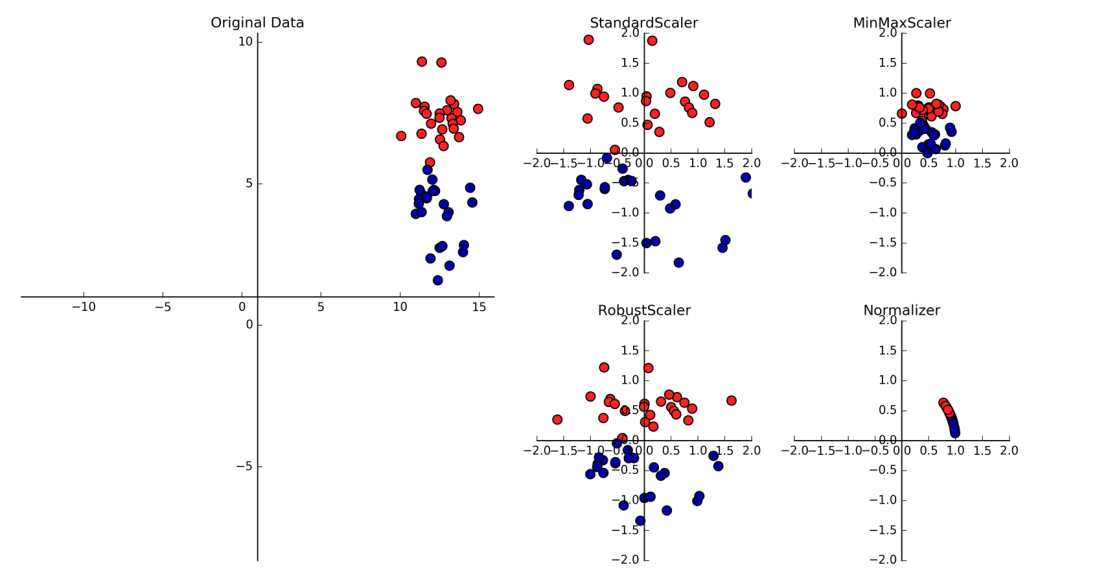
\includegraphics[scale=0.55]{../Imagen_Machine/Simples}
	\caption{Diferentes formas de reescalar y preprocesar un conjunto de datos}
	\label{Simples}
\end{figure}


\subsection{Diferentes tipos de pre-procesamiento de datos}

El primer gráfico de la Figura \ref{Simples} muestra  datos sintéticos con dos clases y  dos caracteristicas. La primera característica (en eje x) se encuentra en un rango  entre 10 y 15, y la segunda característica (en eje y) en un rango entre 1 y 9.\\


Los demás  gráficos muestran cuatro formas diferentes de transformar los datos que  producen  rangos más  estándar.  La función  {\ttfamily StandardScaler} de {\ttfamily scikit-learn} asegura que cada característica tenga  media igual a 0  y  varianza  1, lo que hace que todas las características tengan la misma magnitud; sin embargo, esta escala no garantiza ningún mínimo ni máximo en particular para valores de las características. \\




{\ttfamily RobustScaler} funciona de manera similar a {\ttfamily StandardScaler}  en
que asegura que las propiedades estadísticas para cada característica están en la 
misma escala.  Sin embargo, {\ttfamily RobustScaler} utiliza la mediana y los cuartiles\footnote{\scriptsize	  La mediana de un conjunto de números es el número x tal que la mitad de los números son más pequeños que x y la mitad de los números son más grandes que x. El cuartil inferior es el número x tal que un cuarto de los números son más pequeños que x, y el cuartil superior es el número x tal que un cuarto de los números son más grandes que x.},  en lugar de
media y varianza. Esto hace que  {\ttfamily  RobustScaler} ignore los puntos de datos que son muy
diferente del resto (como errores de medición).  Estos extraños  puntos en los  datos  son llaman valores atípicos, y pueden causar problemas para otras técnicas de escalado.    Por otro lado, el {\ttfamily MinMaxScaler}, cambia los datos de modo que todas las características encuentren exactamente entre 0 y 1.    Para la data bidimensionales esto significa que todos los datos están contenidos dentro del rectángulo creado por el eje x entre 0 y 1 y el eje y entre 0 y 1. \\


Finalmente, el {\ttfamily Normalizer}  hace un tipo muy diferente de re-escalado.  Escala cada punto de datos de tal manera que el vector de característica tiene una longitud euclidiana de 1. En otras palabras, proyecta un punto de datos en el círculo (o esfera, en el caso de dimensiones superiores) con un radio de 1. Esto significa que cada punto de datos se escala por un número diferente (inverso de su longitud). Esta normalización se utiliza a menudo cuando sólo la dirección (o ángulo) de los datos es importate,  y no la longitud del vector de característica.


\subsection{Aplicando transformaciones a la Data}


Ahora que hemos visto lo que hacen los diferentes tipos de transformaciones,  lo aplicaremos  usando  {\ttfamily scikit-learn}.  Usaremos la data de cáncer que vimos en el Capítulo \ref{Cap2}. Los métodos de pre-procesamiento como los escaladores generalmente se aplican  antes de ejecutar un algoritmo  de aprendizaje automático. 

Por ejemplo, digamos que queremos aplicar el kernel SVM  al conjunto de datos de cáncer,  usado {\ttfamily MinMaxscaler} para pre- procesar los datos. Comencemos cargando la data y dividiéndola en los dos conjuntos,  en el de entrenamiento y  prueba (necesitamos los dos conjuntos separados, el de  entrenamiento y el de prueba para evaluar el modelo supervisado que construiremos después del pre-procesamiento):\\

\begin{lstlisting}  % [frame=single]	

In[3]: from sklearn.datasets import load_breast_cancer
       from sklearn.model_selection import train_test_split
       cancer = load_breast_cancer()
   
       X_train, X_test, y_train, y_test = train_test_split(cancer.data,
             cancer.target, random_state=1)
       print(X_train.shape)
       print(X_test.shape)

Out[3]:

    (426, 30)
    (143, 30)

\end{lstlisting}


Recuerde que la dataset  contiene 569  datos, cada uno representado 
por 30 medidas. Dividimos el conjunto de datos en 426 muestras para el  entrenamiento 
y 143 la prueba. \\

Al igual que con los modelos supervisados que construimos anteriormente, primero importamos la clase que implica el pre-procesamiento, y luego lo instanceamos:
 
\begin{lstlisting}

In[4]: from sklearn.preprocessing import MinMaxScaler
   
       scaler = MinMaxScaler()

\end{lstlisting}

Luego ajustamos el escalador usando el método  {\ttfamily fit}, aplicado sobre los datos de entrenamiento. Para  el {\ttfamily MinMaxscaler}, el método  {\ttfamily fit} calcula el valor mínimo y máximo de cada característica en la  data de entrenamiento. A diferencia de los clasificadores y regresores del Capítulo \ref{Cap2}, al escalador sólo se le proporcionan los datos {\ttfamily (X\_train)}  cuando se llama el {\ttfamily fit},  y   {\ttfamily y\_train} no se utiliza:


\begin{lstlisting}  % [frame=single]	
 
In[5]: scaler.fit(X_train)

Out[5]:

   MinMaxScaler(copy=True, feature_range=(0, 1))

\end{lstlisting}



Para aplicar la transformación que acabamos de ver,  es decir, escalar la data de entrenamiento se usa
 el método {\ttfamily transform}   de  {\ttfamily scaler}.
 El método de {\ttfamily transform}  es  usado en  {\ttfamily Scikit-learn} siempre que un modelo devuelve una nueva representación de los datos:\\	
 
\begin{lstlisting}  % [frame=single]

In[6]: # transform data
       X_train_scaled = scaler.transform(X_train)
       # print dataset properties before and after scaling
       print("transformed shape: {}".format(X_train_scaled.shape))
       print("per-feature minimum before scaling:\n {}".format(
              X_train.min(axis=0)))
       print("per-feature maximum before scaling:\n {}".format(
              X_train.max(axis=0)))
       print("per-feature minimum after scaling:\n {}".format(
              X_train_scaled.min(axis=0)))
       print("per-feature maximum after scaling:\n {}".format(
              X_train_scaled.max(axis=0)))

Out[6]:

    transformed shape: (426, 30)
    per-feature minimum before scaling:
     [ 6.98  9.71  43.79  143.50   0.05     0.02   0.   0.   0.11
       0.05  0.12  0.36     0.76   6.80     0.     0.   0.   0.
       0.01  0.    7.93    12.02   50.41  185.20   0.07 0.03  0.
       0.    0.16  0.06]

    per-feature maximum before scaling:
     [ 28.11  39.28  188.5  2501.0    0.16   0.29    0.43     0.2
        0.300  0.100   2.87    4.88  21.98  542.20   0.03     0.14
        0.400  0.050   0.06    0.03  36.04  49.54  251.20  4254.00
        0.220  0.940   1.17    0.29   0.58  0.15]
     
    per-feature minimum after scaling:
     [ 0. 0. 0. 0. 0. 0. 0. 0. 0. 0. 0. 0. 0. 0. 0. 0. 0. 0.
       0. 0. 0. 0. 0. 0. 0. 0. 0. 0. 0. 0.]
    
    per-feature maximum after scaling:
     [ 1. 1. 1. 1. 1. 1. 1. 1. 1. 1. 1. 1. 1. 1. 1. 1. 1. 1.
       1. 1. 1. 1. 1. 1. 1. 1. 1. 1. 1. 1.]

\end{lstlisting}


La data transformada tienen la misma forma que los datos originales; las características simplemente se cambian y se escalan. Puede ver que todas las características están ahora entre 0 y 1, como se desea. \\


Para aplicar el SVM a la data escalada,  necesitamos también  transformar el conjunto de prueba.
Esto se hace de nuevo llamando al método  {\ttfamily transform}, esta vez a { \ttfamily X\_test}:


\begin{lstlisting}  % [frame=single]

In[7]: # transform test data
       X_test_scaled = scaler.transform(X_test)
       # print test data properties after scaling
       print("per-feature minimum after scaling:\n{}".format(
             X_test_scaled.min(axis=0)))
       print("per-feature maximum after scaling:\n{}".format(
          X_test_scaled.max(axis=0)))
   
   Out[7]:
   
   per-feature minimum after scaling:
   [ 0.034  0.023  0.031  0.011  0.141  0.044  0.  0.  0.154  -0.006
    -0.001  0.006  0.004  0.001  0.039  0.011  0.  0.  -0.032  0.007
     0.027  0.058  0.02   0.009  0.109  0.026  0.  0.  -0.    -0.002]
  
   per-feature maximum after scaling:
   [ 0.958  0.815  0.956  0.894  0.811  1.22  0.88  0.933  0.932  1.037
     0.427  0.498  0.441  0.284  0.487  0.739 0.767 0.629  1.337  0.391
     0.896  0.793  0.849  0.745  0.915  1.132 1.07  0.924  1.205  1.631]


\end{lstlisting}

De manera sorprendente, puede ver que para el conjunto de prueba, después de  escalar, el  mínimo  y  máximo no son 0 y 1. ¡Algunas de las características están incluso fuera del rango 0-1!. La explicación es que el {\ttfamily MinMaxscaler} (y todos los otros escaladores) siempre aplica exactamente la misma transformación del entrenamiento y al conjunto de prueba. Esto significa que el método de {\ttfamily transform} siempre resta el mínimo establecido por entrenamiento y se divide por el rango del   entrenamiento, que podría ser diferente del mínimo y rango para el conjunto de prueba.



\subsubsection{Escalado para los Datos de Entrenamiento y Prueba de la misma forma}


 Es importante aplicar exactamente la misma transformación al conjunto de entrenamiento y  prueba, para que el modelo supervisado funcione bien en el conjunto de prueba. El siguiente ejemplo (Figura \ref{IgualScala}) ilustra lo que sucedería si usáramos el mínimo y el rango del conjunto de prueba: 


\begin{lstlisting}  

In[8]: from sklearn.datasets import make_blobs
       # make synthetic data
       X, _ = make_blobs(n_samples=50, centers=5, random_state=4, cluster_std=2)
       # split it into training and test sets
       X_train, X_test = train_test_split(X, random_state=5, test_size=.1)
   
       # plot the training and test sets
       fig, axes = plt.subplots(1, 3, figsize=(13, 4))

       axes[0].scatter(X_train[:, 0], X_train[:, 1],
                       c=mglearn.cm2(0), label="Training set", s=60)
       axes[0].scatter(X_test[:, 0], X_test[:, 1], marker='^',
                       c=mglearn.cm2(1), label="Test set", s=60)
       axes[0].legend(loc='upper left')
       axes[0].set_title("Original Data")
   
       # scale the data using MinMaxScaler
       scaler = MinMaxScaler()
       scaler.fit(X_train)
       X_train_scaled = scaler.transform(X_train)
       X_test_scaled = scaler.transform(X_test)
   
       # visualize the properly scaled data
       axes[1].scatter(X_train_scaled[:, 0], X_train_scaled[:, 1],
                       c=mglearn.cm2(0), label="Training set", s=60)
       axes[1].scatter(X_test_scaled[:, 0], X_test_scaled[:, 1], marker='^',
                       c=mglearn.cm2(1), label="Test set", s=60)
       axes[1].set_title("Scaled Data")
   
       # rescale the test set separately
       # so test set min is 0 and test set max is 1
       # No haga esto! Solo para proposito de ilustracion. 
       test_scaler = MinMaxScaler()
       test_scaler.fit(X_test)
       X_test_scaled_badly = test_scaler.transform(X_test)
   
       # visualize wrongly scaled data
       axes[2].scatter(X_train_scaled[:, 0], X_train_scaled[:, 1],
                       c=mglearn.cm2(0), label="training set", s=60)
       axes[2].scatter(X_test_scaled_badly[:, 0], X_test_scaled_badly[:, 1],
                       marker='^', c=mglearn.cm2(1), label="test set", s=60)
       axes[2].set_title("Improperly Scaled Data")
   
       for ax in axes:
           ax.set_xlabel("Feature 0")
           ax.set_ylabel("Feature 1")

\end{lstlisting} 


\begin{figure}[h!]
	\centering
	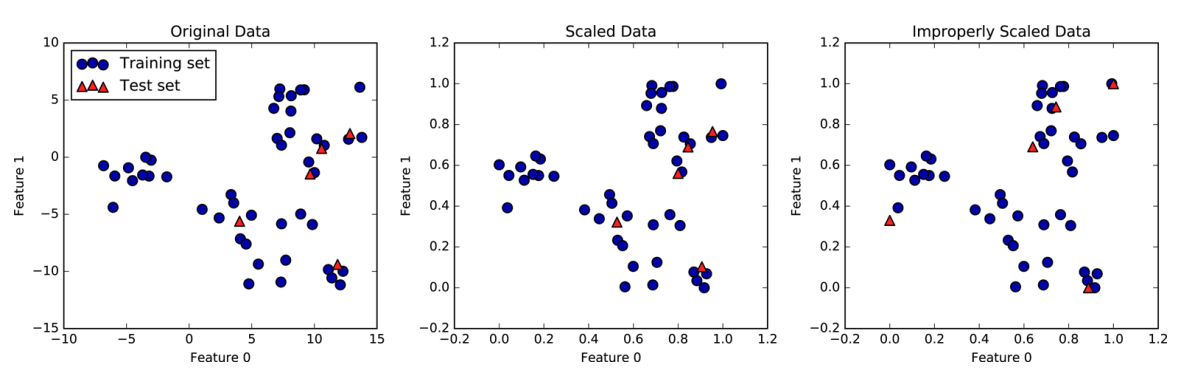
\includegraphics[scale=0.545]{../Imagen_Machine/IgualScala}
	\caption{Efecto del escalado en la data de entrenamiento y prueba, a la izquierda data originales, en el centro datos  escalados juntos, y  a la derecha escalado  por separado}
	\label{IgualScala}
\end{figure}

El primer gráfico es un conjunto de datos bidimensionales sin escalar, los puntos del conjunto de entrenamiento se presentan como círculos y los de prueba  como triángulos. El segundo gráfico    son los mismos datos, pero escalado usando el {\ttfamily MinMaxscaler}. Aquí, llamamos el {\ttfamily fit}  sobre el entrenamiento, y luego llamado transformación en data de entrenamiento y prueba.  Se puede ver que la data en el segundo  gráfico   se ve idéntico a la primera; sólo las marcas en los ejes han cambiado. Ahora todas las características están entre 0 y 1. También se observa que los valores mínimos y máximos de las características para los datos de prueba (los triángulos) no son 0 y 1.\\

\vspace{-2cm}	
\hspace{-1cm}
{\fcolorbox{red}{white}{ 		
		
		\begin{minipage}[16cm]{13.5cm}    %   centrado, largo y ancho                {14cm} 
			\vspace{0.4cm}	
			
			
			\begin{center}
				{\bf Atajos y Alternativas Eficientes}
			\end{center}	
			
			
			
			Con frecuencia, se quiere ajustar un modelo sobre algún conjunto de datos, y luego transformarlo.
			Esta es una tarea muy común, el cual  puede ser calculado más eficientemente  por un simplemente llamando {\ttfamily fit}  y  luego  transformar. Para este caso, todos los modelos que tienen un método de {\ttfamily transform}  también tienen un método {\ttfamily fit\_transform}. Veamos el próximo ejemplo utilizando el método  {\ttfamily Standardscaler}:\\
			
			
			{\ttfamily   	{\scriptsize{  	 
						
						In[9]:\\		
						{ \color{blue}									
							
							\hspace{0.3cm}	from sklearn.preprocessing import StandardScaler 
							
							\hspace{0.3cm}	scaler = StandardScaler() 
							
							\hspace{0.3cm}	\# calling fit and transform in sequence (using method chaining) 
							
							\hspace{0.3cm}	X\_scaled = scaler.fit(X).transform(X)  
							
							\hspace{0.3cm}	\# same result, but more efficient computation  \vspace{-0.2cm}
							
							\hspace{0.3cm}	X\_scaled\_d = scaler.fit\_transform(X)) }  \\}}}
			
			
			Escalar con    {\ttfamily fit\_transform} no es necesariamente el más eficiente para todos los modelos,  pero es una buena práctica utilizar este método cuando se trata de transformar la data de entrenamiento.\\			
			
		\end{minipage}
}}  \\

El tercer  gráfico  muestra lo que sucedería si escalamos el conjunto de entrenamiento y prueba por separado. En este caso, los valores mínimos y máximos de característica para el entrenamiento y el de  prueba  son  0 y 1.   Pero ahora el conjunto de datos parece diferente. Los puntos de prueba se movieron incongruentemente al conjunto de entrenamiento, ya que fueron escalados de manera diferente. Cambiamos la disposición de los datos de una manera arbitraria.  Claramente esto no es lo que queremos hacer. \\

Otra forma de ilustrar este inconveniente es la siguiente, imaginen que su conjunto de prueba tiene un solo punto. No hay manera de escalar un solo punto correctamente, para cumplir con los requerimientos mínimos y máximos del {\ttfamily MinMaxscaler}. El tamaño de su conjunto de pruebas no debe cambiar su procesamiento.\\

%\newpage





\subsection{Efecto del preprocesamiento en Aprendizaje \\ Supervisado}


Ahora volvamos a la data de cáncer y veamos el efecto del uso del escalador  {\ttfamily MinMaxscaler} en el aprendizaje de  SVC (esta es una forma diferente de escalar de la misma forma que hicimos en el capítulo \ref{Cap2}). Primero, ajustemos el SVC sobre  los datos originales para luego comparar:


\begin{lstlisting}  % [frame=single]	

In[10]: from sklearn.svm import SVC
   
        X_train, X_test, y_train, y_test = train_test_split(cancer.data, 
               cancer.target, random_state=0)
        svm = SVC(C=100)
        svm.fit(X_train, y_train)
        print("Test set accuracy: {:.2f}".format(svm.score(X_test, y_test)))

Out[10]:

    Test set accuracy: 0.63

\end{lstlisting} 


Ahora, escalamos la data usando {\ttfamily MinMaxScaler} antes de ajustar el modelo SVC:


\begin{lstlisting}  

In[11]: # preprocessing using 0-1 scaling
        scaler = MinMaxScaler()
        scaler.fit(X_train)
        X_train_scaled = scaler.transform(X_train)
        X_test_scaled = scaler.transform(X_test)
   
        # learning an SVM on the scaled training data
        svm.fit(X_train_scaled, y_train)
        # scoring on the scaled test set
        print("Scaled test set accuracy: {:.2f}".format(
               svm.score(X_test_scaled, y_test)))

Out[11]:

    Scaled test set accuracy: 0.97

\end{lstlisting} 

Como vimos antes, el efecto de escalar los datos es muy significativo. Sin embargo,
escalar los datos no implica ninguna complicación matemática, una buena  práctica usar las
herramientas que provee  {\ttfamily scikit-learn}  para escalar, en lugar de reimplementarlos por si mismo,
evitando  cometer errores, pues es fácil  equivocarse  aún en estos simples cálculos.

También se puede  reemplazar fácilmente   un algoritmo preprocesador con otro cambiando la
clase a usar, como todas las clases pre-procesadas tiene la misma interfaz, que  consisten  en
 los  métodos {\ttfamily fit}  y  {\ttfamily  transform}:\\



\begin{lstlisting}  %[basicstyle=\scriptsize] % [ frame=single]

In[12]: # preprocessing using zero mean and unit variance scaling
        from sklearn.preprocessing import StandardScaler
        scaler = StandardScaler()
        scaler.fit(X_train)
        X_train_scaled = scaler.transform(X_train)
        X_test_scaled = scaler.transform(X_test)
   
        # learning an SVM on the scaled training data
        svm.fit(X_train_scaled, y_train)
        # scoring on the scaled test set
        print("SVM test accuracy: {:.2f}".format(
               svm.score(X_test_scaled, y_test)))

Out[12]:

    SVM test accuracy: 0.96

\end{lstlisting} 

Ahora que hemos visto qué tan simple son las transformaciones para preprocesar  los datos, podemos ir
 hacia transformaciones más interesantes usandas en el aprendizaje no supervisado.


\section{Reducción de Dimensionalidad, Extracción de Característica, y  Aprendizaje Múltiple}

Como discutimos anteriormente, transformar la data usando aprendizaje no supervisión puede tener
muchas motivaciones. Entre las motivaciones más comunes tenemos la visualización, datos a comprimir, o  en busca de una representación que sea más informativa para el  procesamiento.\\

El análisis de Componentes Principales es  uno de los algoritmos más simple y ampliamente usados en   el aprendizaje no supervisado; en este texto consideraremos  también otros dos algoritmos: factorización Matricial no negativa (non-negative matrix factorization   NMF), el cual sirve comúnmente para extracción de característica, y t-SNE, que se emplea  comúnmente para visualizar la dispersión  en gráficos  de dos dimensiones.


\subsection{Análisis de componentes principales (PCA)}


El análisis de componentes principales es un método que rota la data de forma tal que las
 características resultantes (rotadas) son estadísticamente no correlacionadas. Esta rotación es 
frecuentemete seguida por la selección de un subconjunto de características nuevas, de acuerdo   
a su importancia  para explicar la data.   El siguiente ejemplo (Figura \ref{CompontPric}) ilustra el efecto de PCA sobre la dataset  sintética con dos dimensiones:\\


\begin{lstlisting}  % [frame=single]	

In[13]: mglearn.plots.plot_pca_illustration()

\end{lstlisting} 



\begin{figure}[h!]
	\centering
	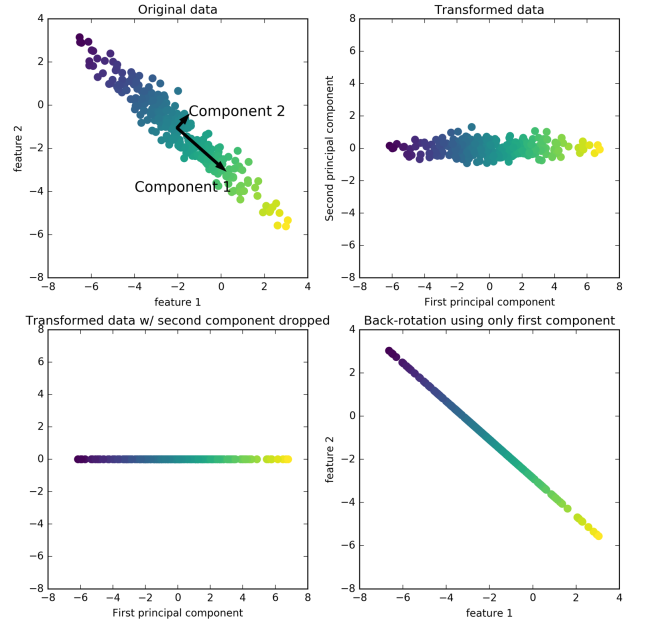
\includegraphics[scale=0.95]{../Imagen_Machine/CompontPric}
	\caption{Transformación de la  Data con PCA}
	\label{CompontPric}
\end{figure}

El primer gráfico (parte izquierda superior) muestra los datos originales, con puntos coloreados para hacer 
distinción entre ellos.   El algoritmo procede  primero para encontrar la dirección de máxima varianza, y la
etiqueta  como  "{}Componente 1{}". { }  Ésta es la dirección (o el vector) en la data que contiene más información, en otras palabras, la dirección a lo largo de la cual las características están más  correlacionadas unas con otras. El algoritmo encuentra la dirección que contiene  mayor  información,  y la hace  ortogonal (ángulo recto) para la primera dirección. En el caso de dos dimensiones, hay sólo una orientación posible que está en un ángulo recto, pero en espacios de  alta  dimensión podrían ser  muchas direcciones  (infinitamente) ortogonales.   Aunque las dos componentes se trazan como flechas, realmente no tiene importancia donde la va la cabeza y la cola;  pudimos haber  graficado la primera  componente del centro  hasta la izquierda superior en lugar abajo a la derecha inferior.  Las direcciones que se encuentran  en  este proceso son  llamadas  componentes principales,  son las direcciones principales de la varianza de  la  data. En general, hay tantas componentes principales como características originales haya.\\


El segundo gráfico (parte superior derecha) muestra la misma data, pero ahora rotando de tal manera que la primera componente principal se alinea con el eje de las abscisas (eje x) y la segunda componente principal se alinea con eje de las ordenadas (eje y).  Antes de la rotación,  la media fue sustraída de la data, así que la data transformada es centrada  en cero. En la representación de las nuevas características (rotada) encontradas por PCA, los dos ejes  son no correlacionados, lo que significa que  la matriz de correlación de la data en esta representación es cero excepto en  la diagonal.

Podemos usar  PCA  para  reducir la  dimensionalidad conservando sólo a algunos de las componentes del principales.   En este ejemplo, podríamos quedarnos sólo con la primer componente principal, como se 
muestra en el tercer gráfico de la Figura \ref{CompontPric} (parte inferior izquierda). Esto reduce la dataset de dos dimensiones una  dataset de una  dimensión.  

Observe,  que en lugar de conservar  una de las características originales, encontramos la dirección más interesante (esquina izquierda superior  a esquina derecha inferior en el primer gráfico) y se conserva esta dirección, como la primer componente principal. \\


Finalmente, podemos deshacer el proceso de rotación y añadir (sumar)  la media  a los datos.
Este resultado se muestra en el último gráfico  en de la Figura \ref{CompontPric}. Ahora los puntos están 
 en el espacio de características original, pero conservamos  sólo la información contenida en la primer componente principal.
 
Esta transformación se usa algunas veces para remover efectos de ruido en los datos o para 
visualizar qué parte de la información es retenida usando los componentes principales.


\subsubsection{Aplicándo PCA a la  data de cáncer para visualización}


Una de las aplicaciones más comunes de PCA es para visualizar data de alta dimensiones. Como vimos en Capítulo \ref{Cap1}, es difícil de crear gráficos  de dispersión de datos que tiene más de dos características.  Para  el caso de la dataset Iris, se crearon   gráficos con  pares de característica (Figura \ref{Iris}),    generando un cuadro parcial de la data, mostrándo todas las posibles combinaciones de dos en dos características.   Pero si queremos ver la dataset de Cáncer Breast, aún usando  gráficos con  pares de característica no es viable. Esta dataset tiene 30 características, lo cual resultaría  ¡30 * 14 = 420 gráficos  de dispersión   !Nunca podríamos vernos en detalle todos estos gráficos, y mucho menos  intentar comprenderlos.



Hay una visualización aun más simple que podemos usar,  computando histogramas de
cada uno de las características para las dos clases, benigno y maligno (Figura \ref{Histogram} ):\\

\begin{lstlisting}  % [frame=single]	

In[14]: fig, axes = plt.subplots(15, 2, figsize=(10, 20))
        malignant = cancer.data[cancer.target == 0]
        benign = cancer.data[cancer.target == 1]
   
        ax = axes.ravel() 

        for i in range(30):
            _, bins = np.histogram(cancer.data[:, i], bins=50)
            ax[i].hist(malignant[:, i], bins=bins, color=mglearn.cm3(0), 
                        alpha=.5)
            ax[i].hist(benign[:, i], bins=bins, color=mglearn.cm3(2), 
                        alpha=.5)
            ax[i].set_title(cancer.feature_names[i])
            ax[i].set_yticks(())
        ax[0].set_xlabel("Feature magnitude")
        ax[0].set_ylabel("Frequency")
        ax[0].legend(["malignant", "benign"], loc="best")
        fig.tight_layout()


\end{lstlisting} 



\begin{figure}[!h]
	\centering
	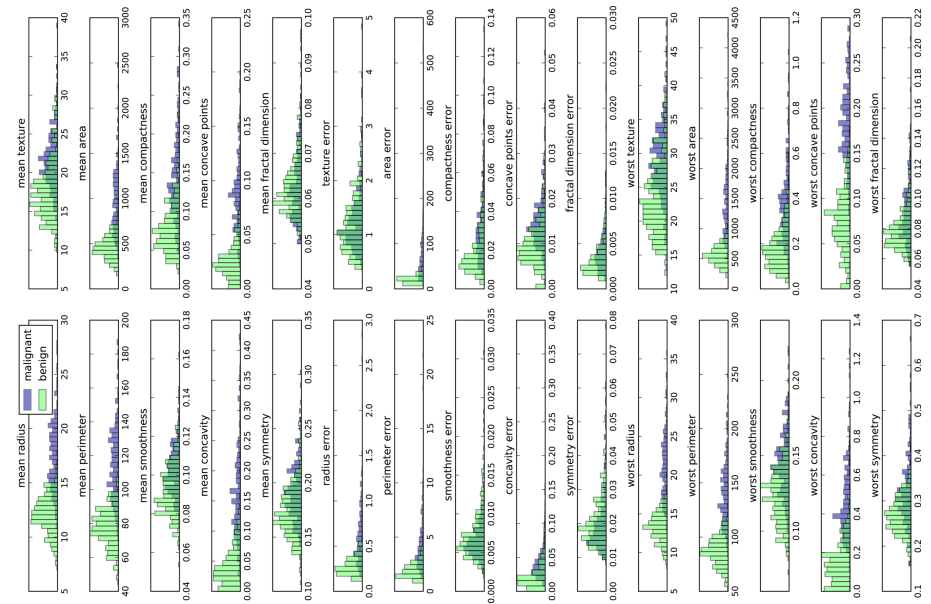
\includegraphics[width=17cm, height=13.6cm, angle=-90]{../Imagen_Machine/Histogram}
	\caption{Histogramas de características por clase sobre la data de cáncer de mama}
	\label{Histogram}
\end{figure}


La figura \ref{Histogram} se presenta los histogramas de frecuencia  creados para cada  características y sus dos clases, en cada gráfico se superpone dos histogramas, uno para la clase benigna (azul) y el otro para  la clase maligna (rojo).   Esto nos da alguna idea de cómo  cada característica esta distribuida respecto a las  dos clases, y nos permite  hacer conjeturas en cuanto a qué características  distinguen mejor las muestras malignas y benignas. 






  Por ejemplo, la característica  “{}smoothness error”{}  parece  poco informativo, porque los dos histogramas  se superponen  en su mayoría, mientras que la característica  “{}worst concave points”{}  parece más informativo, ya que  los histogramas son bastantes  disjuntos.\\


Sin embargo, este gráfico no nos muestra nada acerca de las interacciones entre variables y cómo éstas se relacionan con las clases. Usando PCA, podemos capturar las interacciones principales y obtener una imagen un poco más completa.   Podemos encontrar las dos primeras componentes principales, y visualizar los datos en este nuevo espacio bidimensional en un gráfico de dispersión. \\

Antes de aplicar PCA, escalamos la data para que cada característica tenga varianza igual a la  unidad usando {\ttfamily Standardscaler}: 


\begin{lstlisting}  % [frame=single]	


In[15]: from sklearn.datasets import load_breast_cancer
        cancer = load_breast_cancer()
        scaler = StandardScaler()
        scaler.fit(cancer.data)
        X_scaled = scaler.transform(cancer.data)

\end{lstlisting} 

 Aplicar la  transformación de PCA  es tan simple como aplicarle una 
 transformación de preprocesamiento a la data.  Ahora instanciamos el objeto PCA, para  buscar las componentes principales mediante el método {\ttfamily fit}, se  aplica la rotación y la reducción de dimensionalidad haciendo uso de {\ttfamily transform}.

 Por defecto, PCA sólo rota (y los cambios) la data, pero conserva todos los componentes principales. Para reducir la dimensionalidad de la data, necesitamos especificar cuántos componentes queremos conservar al crear el objeto PCA:


\begin{lstlisting}  % [frame=single]	


In[16]: from sklearn.decomposition import PCA
        # keep the first two principal components of the data
        pca = PCA(n_components=2)
        # fit PCA model to breast cancer data
        pca.fit(X_scaled)
   
        # transform data onto the first two principal components
        X_pca = pca.transform(X_scaled)
        print("Original shape: {}".format(str(X_scaled.shape)))
        print("Reduced shape: {}".format(str(X_pca.shape)))

Out[16]:

    Original shape: (569, 30)
    Reduced shape: (569, 2)


\end{lstlisting} 

Ahora podemos graficar las primeras dos componentes principales (Figura \ref{Com2Pric}):


\begin{lstlisting}  

In[17]: # plot first vs. second principal component, colored by class
        plt.figure(figsize=(8, 8))
        mglearn.discrete_scatter(X_pca[:, 0], X_pca[:, 1], cancer.target)
        plt.legend(cancer.target_names, loc="best")
        plt.gca().set_aspect("equal")      
        plt.xlabel("First principal component")
        plt.ylabel("Second principal component")

\end{lstlisting} 


\begin{figure}[!h]
	\centering
	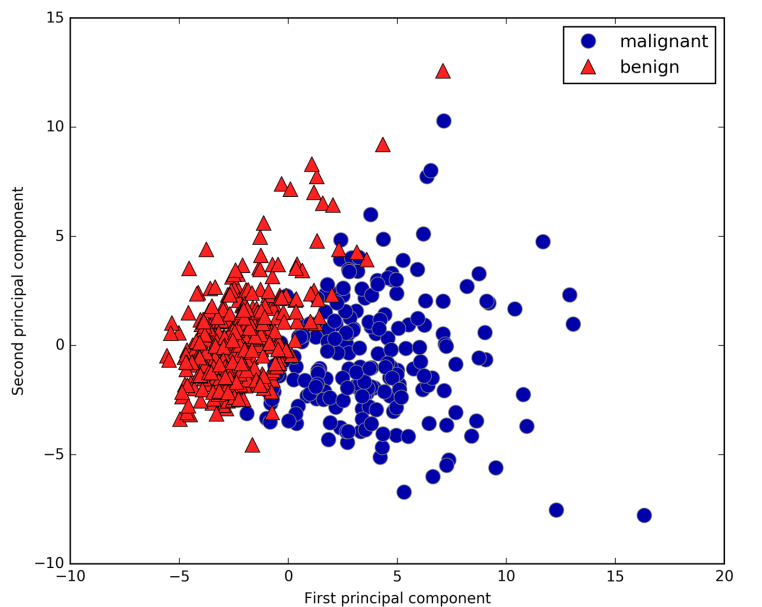
\includegraphics[scale=0.65]{../Imagen_Machine/Com2Pric}
	\caption{Diagrama de dispersión bidimensional de la data de
		 cáncer de mama, utilizando las dos primeras componentes principales}
	\label{Com2Pric}
\end{figure}


Es importante tener en cuenta que PCA es un método no supervisado y no utiliza ninguna clase
información cuando encuentra la rotación, simplemente toma en cuenta  las correlaciones en la data.
El diagrama de dispersión de la figura \ref{Com2Pric}, muestra la  primera componente principal contra 
la  segunda,  y luego usa la información de la clase para colorear los puntos.
Se puede ver  las dos clases separadas bastante bien en este espacio bidimensional.
Esto nos lleva a creer que incluso un clasificador lineal (que aprendería una línea en este
espacio) podría hacer un trabajo razonablemente bueno para distinguir las dos clases.
 También podemos ver que los puntos malignos (azul) están más extendidos que los puntos benignos (rojo), algo que ya habiamos visto en los histogramas  Figura \ref{Histogram}.\\



Una desventaja de PCA es que los dos ejes en el gráfico generalmente  no son muy fáciles de interpretar.
Las componentes principales corresponden a las direcciones de la data  original, por lo que son
combinaciones de las características originales. Sin embargo, estas combinaciones suelen ser muy
complejas, como veremos  más adelante. Durante la corrida o ejecusión  las componentes principales son almacenadas en el atributo  {\ttfamily components\_}  del objeto PCA:\\



\begin{lstlisting}  % [frame=single]	

In[18]: print("PCA component shape: {}".format(pca.components_.shape))

Out[18]:

   PCA component shape: (2, 30)

\end{lstlisting} 

Cada fila en el atributo {\ttfamily components\_  }  corresponde a una componente principal, y están ordenados por  su importancia (la  primera componente principal va primero, y así sucesivamente). Las columnas
corresponden  al atributo original de las características de los PCA en este ejemplo,  “{}mean
radius{}”,   “{}mean texture”{},  y así sucesivamente. 

Veamos el contenido de las componentes {\ttfamily components\_}:

\begin{lstlisting} 

In[19]: print("Las dos componentes PAC:\n{}".format(pca.components_))

Out[19]:
   
    Las dos componentes PAC:
    [[ 0.219  0.104  0.228  0.221  0.143  0.239  0.258  0.261  0.138  0.064
       0.206  0.017  0.21   0.203  0.015  0.17   0.154  0.183  0.042  0.103
       0.228  0.104  0.237  0.225  0.128  0.21   0.229  0.251  0.123  0.132]
     [-0.234 -0.06  -0.215 -0.231  0.186  0.152  0.06  -0.035  0.19   0.367
      -0.106  0.09  -0.089 -0.152  0.204  0.233  0.197  0.13   0.184  0.28
      -0.22  -0.045 -0.2   -0.219  0.172  0.144  0.098 -0.008  0.142  0.275]]

\end{lstlisting}También podemos visualizar los coeficientes usando un mapa caliente (Figura \ref{Caliente}), que podría ser más fácil de entender:

\begin{lstlisting} 

In[20]: plt.matshow(pca.components_, cmap='viridis')
        plt.yticks([0, 1], ["First component", "Second component"])
        plt.colorbar()
        plt.xticks(range(len(cancer.feature_names)),
                   cancer.feature_names, rotation=60, ha='left')
        plt.xlabel("Feature")
        plt.ylabel("Principal components")

\end{lstlisting} 


\begin{figure}[h!]
	\centering
	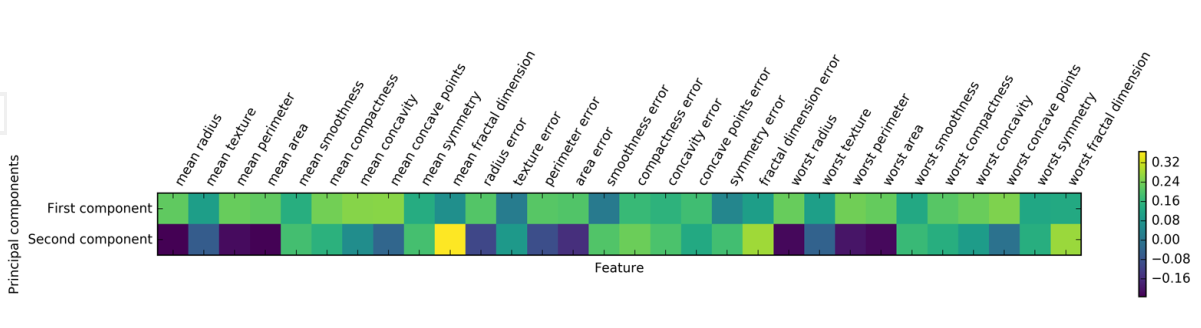
\includegraphics[scale=0.525]{../Imagen_Machine/Caliente}
	\caption{Mapa caliente de los dos primeros componentes principales en  la dataset de Cáncer de Mama}
	\label{Caliente}
\end{figure}



Puede ver que en la primer componente, todas las características  tienen el mismo signo ( positivo, pero como señalamos anteriormente, no importa en qué dirección apunte la flecha).   Eso significa que hay una correlación general entre todas las características. En caso de un valor o medida alta, es probable las demás  también sean  altas. La  segunda componente tiene signos diferentes.

Observe que  ambas componentes involucran las 30 características;  esta mezcla de todas las características es lo que hace tan difícil explicar los ejes en la Figura \ref{Caliente}.
 
\subsubsection{Caracteres propios para extracción de características \\  (Eigenfaces\index{eigenface})}

%autovalores

Otra aplicación de PCA que mencionamos anteriormente es la extracción de características.  La idea detrás de la extracción de características es la posibilidad de encontrar una representación de los datos que se adapta mejor al análisis, que la representación original. Un buen
ejemplo de una aplicación donde la extracción de características es útil es con imágenes.   Las imágenes están formados por píxeles, generalmente almacenados como intensidades de rojo, verde y azul (RGB).  Los objetos en las imágenes generalmente están formados por miles de píxeles, y sólo juntos son  tienen  significado.\\

 Ejemplificaremos la extracción de características  con  una aplicación de PCA, sobre las imágenes de caras etiquetadas de la dataset Wild.   Este conjunto de datos contiene imágenes de caras de celebridades descargadas de Internet,  incluye rostros de políticos, cantantes, actores y atletas de principios de la década del 2000.  Usamos versiones en escala de grises de estas imágenes,  y reducimos  para  un procesamiento más rápido.  Algunas de las imágenes se muestran en la Figura \ref{Caras1}:

\begin{lstlisting} 

In[21]: from sklearn.datasets import fetch_lfw_people
        people = fetch_lfw_people(min_faces_per_person=20, resize=0.7)
        image_shape = people.images[0].shape
   
        fix, axes = plt.subplots(2, 5, figsize=(15, 8),
                                  subplot_kw={'xticks': (), 'yticks': ()})
        for target, image, ax in zip(people.target, people.images, axes.ravel()):
            ax.imshow(image)
            ax.set_title(people.target_names[target])

\end{lstlisting} 



\begin{figure}[h!]
	\centering
	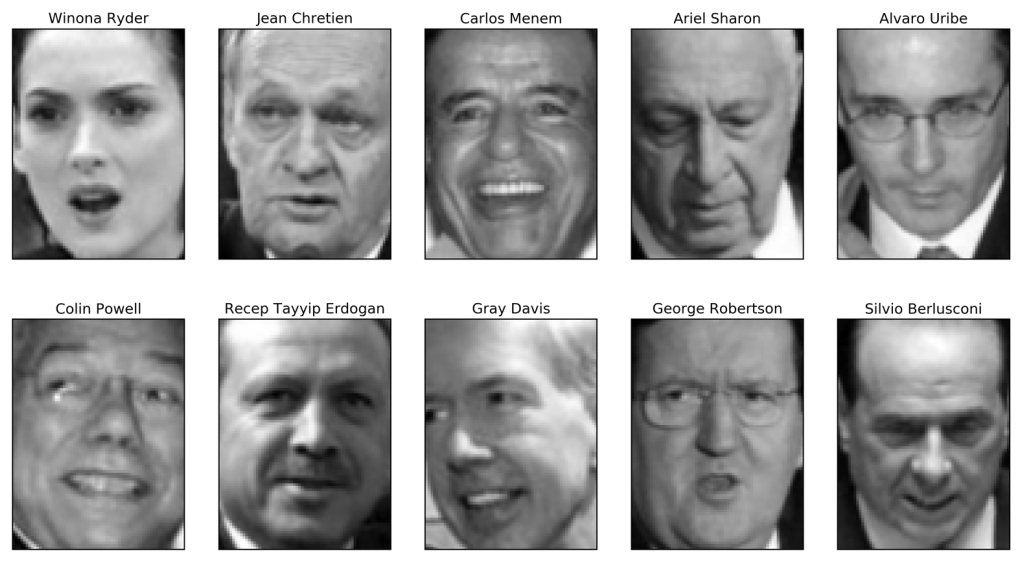
\includegraphics[scale=0.63]{../Imagen_Machine/Caras1}
	\caption{Algunas imágenes de las caras etiquetadas en la dataset de Wild}
	\label{Caras1}
\end{figure}



Hay 3.023 imagenes, cada una con 87x65 píxeles de tamaño, que pertenecen a 62 personas diferentes:


\begin{lstlisting} 


In[22]: print("people.images.shape: {}".format(people.images.shape))
        print("Number of classes: {}".format(len(people.target_names)))

Out[22]:

    people.images.shape: (3023, 87, 65)
    Number of classes: 62

\end{lstlisting} 

La dataset  esta un poco sesgada, sin embargo,  contiene una gran cantidad de imágenes de George W. Bush y Colin Powell, como se puede ver en la figura \ref{Caras1}:\\

\begin{lstlisting}  % [frame=single]	


In[23]: # contar cuantas veces aparece cada objetivo
        counts = np.bincount(people.target)
        # print counts next to target names
        for i, (count, name) in enumerate(zip(counts, people.target_names)):
            print("{0:25} {1:3}".format(name, count), end=' ')
            if (i + 1) % 3 == 0:
                print()



Out[23]:

    Alejandro Toledo        39   Alvaro Uribe               35
    Amelie Mauresmo         21   Andre Agassi               36
    Angelina Jolie          20   Arnold Schwarzenegger      42
    Atal Bihari Vajpayee    24   Bill Clinton               29
    Carlos Menem            21   Colin Powell              236
    David Beckham           31   Donald Rumsfeld           121
    George W Bush          530   George Robertson           22
    Gerhard Schroeder      109   Gloria Macapagal Arroyo    44
    Gray Davis              26   Guillermo Coria            30
    Hamid Karzai            22   Hans Blix                  39
    Hugo Chavez             71   Igor Ivanov                20
    [...]                   [...]
    Laura Bush              41   Lindsay Davenport          22
    Lleyton Hewitt          41   Luiz Inacio Lula da Silva  48
    Mahmoud Abbas           29   Megawati Sukarnoputri      33
    Michael Bloomberg       20   Naomi Watts                22
    Nestor Kirchner         37   Paul Bremer                20
    Pete Sampras            22   Recep Tayyip Erdogan       30
    Ricardo Lagos           27   Roh Moo-hyun               32
    Rudolph Giuliani        26   Saddam Hussein             23
    Serena Williams         52   Silvio Berlusconi          33
    Tiger Woods             23   Tom Daschle                25
    Tom Ridge               33   Tony Blair                144
    Vicente Fox             32   Vladimir Putin             49
    Winona Ryder            24

\end{lstlisting}



Para hacer la data  menos sesgada, sólo tomaremos  50 imágenes de cada persona (de lo contrario, la extracción de características sería abrumadora por la probabilidad de George W. Bush):\\


\begin{lstlisting}  
In[24]: mask = np.zeros(people.target.shape, dtype=np.bool)
        for target in np.unique(people.target):
            mask[np.where(people.target == target)[0][:50]] = 1
   
        X_people = people.data[mask]
        y_people = people.target[mask]
   
        # scale the grayscale values to be between 0 and 1
        # instead of 0 and 255 for better numeric stability
        X_people = X_people / 255.


\end{lstlisting} 

Una tarea común en reconocimiento facial es preguntar si una cara no vista anteriormente pertenece a una persona conocida de una base de datos. Esto tiene aplicaciones en la colección de fotos, redes sociales y aplicaciones de seguridad. Una manera de resolver este problema sería construir un clasificador donde cada persona es una clase separada. Sin embargo, por lo general hay muchas personas diferentes en las bases de datos  de cara, y muy pocas imágenes de la misma persona (es decir, muy pocos ejemplos para entrenamiento por clase). Eso hace que sea difícil entrenar a la mayoría de los clasificadores. Además, casi siempre se quiere que la solución al problema tenga la capacidad de añadir fácilmente nuevos datos, en este caso imágenes de gente nueva, sin necesidad de volver a entrenar el modelo. Una solución simple es utilizar un clasificador del un vecino más cercano que busca la imagen más similar a la cara que está clasificando. Este clasificador podría funcionar en principio con un sólo ejemplar de entrenamiento por clase. \\

Veamos qué tan bien  funciona  el clasificador {\ttfamily Kneighborsclassifier}:\\

\begin{lstlisting} 
In[25]: from sklearn.neighbors import KNeighborsClassifier
        # split the data into training and test sets
        X_train, X_test, y_train, y_test = train_test_split(
              X_people, y_people, stratify=y_people, random_state=0)
        # build a KNeighborsClassifier using one neighbor
        knn = KNeighborsClassifier(n_neighbors=1)
        knn.fit(X_train, y_train)
        print("Test set score of 1-nn: {:.2f}".format(knn.score(X_test, y_test)))

Out[25]:

    Test set score of 1-nn: 0.27

\end{lstlisting} 


En este caso se obtiene  una exactitud del 26,6\%, que en realidad no es tan malo para un problema de  clasificación de 62 clases  (tratar de adivinar al azar le daría alrededor de 1/62 = 1.5\% de exactitud),  pero tampoco es gran cosa.   Sólo identificamos correctamente a una persona cada cuatro veces.
 
  Aquí es donde entra en juego la técnica de PCA. Calcular las distancias en el espacio de píxeles original es una mala manera de medir la similitud entre caras. Cuando se usa una representación de píxeles para comparar dos imágenes, comparamos la escala de grises de cada píxel individual con el valor del píxel en la posición correspondiente en la otra imagen.  Esta representación es muy diferente de cómo los humanos interpretarían la imagen de un rostro, y es difícil capturar los rasgos faciales usando esta representación en bruto.   Por ejemplo, usando distancias de píxeles significa cambiar  una cara por  un píxel que corresponde a la derecha, esto es un cambio drástico, con una representación completamente diferente.  Con  el uso de distances a lo largo de los componentes principales se espera que  mejore la  exactitud.   En este caso, habilitamos la opción de blanqueaqueo de PCA, que re-escala los componentes principales para tener la misma escala. Esto es lo mismo que usar {\ttfamily StandardScaler} después de la transformación. Utilizando nuevamente la data  de la Figura \ref{CompontPric}, el blanqueo corresponde no sólo a rotar los datos, sino también re-escalar para que el gráfico central sea un círculo en lugar de una elipse (ver figura \ref{Blanqueo}):\\


\begin{lstlisting}  % [frame=single]	

In[26]: mglearn.plots.plot_pca_whitening()

\end{lstlisting} 



\begin{figure}[h!]
	\centering
	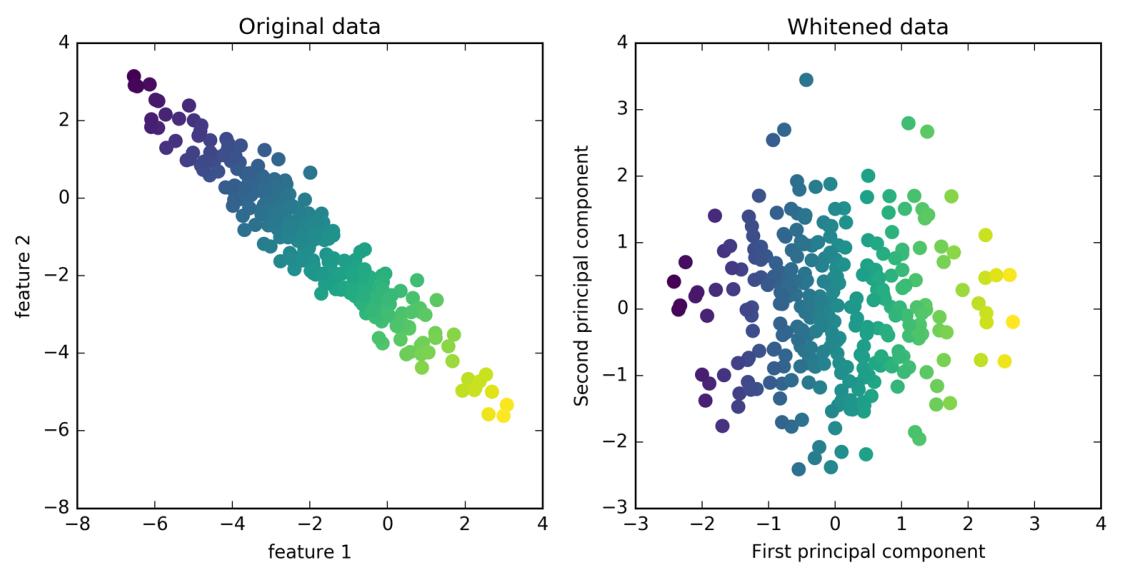
\includegraphics[scale=0.55]{../Imagen_Machine/Blanqueo}
	\caption{Transformación de datos con PCA mediante blanqueamiento}
	\label{Blanqueo}
\end{figure}


Ajustamos el objeto {\ttfamily PCA}  a los datos de entrenamiento y extraemos las primeras 100 componentes principales. Luego transformamos los datos de entrenamiento y prueba:\\

\begin{lstlisting}  % [frame=single]	

In[27]: pca = PCA(n_components=100, 
                   whiten=True, random_state=0).fit(X_train)
        X_train_pca = pca.transform(X_train)
        X_test_pca = pca.transform(X_test)
   
        print("X_train_pca.shape: {}".format(X_train_pca.shape))

Out[27]:

    X_train_pca.shape: (1537, 100)

\end{lstlisting} 

La nueva  data tienen 100 características, las primeras 100 componentes principales. Ahora, podemos usar la nueva representación para clasificar las imágenes usando el clasificador de vecinos más cercanos con un vecino (one-nearest-neighbors):

\begin{lstlisting}  	

In[28]: knn = KNeighborsClassifier(n_neighbors=1)
        knn.fit(X_train_pca, y_train)
        print("Test set accuracy: {:.2f}".format(
                knn.score(X_test_pca, y_test)))

Out[28]:

    Test set accuracy: 0.36


\end{lstlisting} 



La exctitud  mejoró  significativamente, del  26,6\%   al   35,7\%,   confirmando nuestra intuición de que los componentes principales podrían proporcionar una mejor representación de la data.


Para los datos de imagen, también podemos visualizar fácilmente los principales componentes que se encuentran. Recuerde que los componentes corresponden a las direcciones en el espacio de entrada. El espacio de entrada aquí  es 50x37  píxeles de la imagen  en  escala de grises, así que las direcciones dentro de este espacio son también 50x37  píxeles de la imagen  en  escala de grises.\\

 Veamos el  primer par de componentes principales (Figura \ref{PrimerPar}):\\



\begin{lstlisting}  % [frame=single]	

In[29]: print("pca.components_.shape: {}".format(pca.components_.shape))

Out[29]:
    
    pca.components_.shape: (100, 5655)

In[30]: fix, axes = plt.subplots(3, 5, figsize=(15, 12),
                                 subplot_kw={'xticks': (), 'yticks': ()})

        for i, (component, ax) in enumerate(zip(pca.components_, 
                                                 axes.ravel())):
            ax.imshow(component.reshape(image_shape),
                   cmap='viridis')
            ax.set_title("{}. component".format((i + 1)))

\end{lstlisting} 



	
Aunque ciertamente no podemos entender todos los aspectos de estas componentes,  podemos suponer cuales aspectos de las imágenes faciales son capturando por algunas de las componentes.  La primera componente  parece codificar principalmente el contraste entre la cara y el fondo, la segunda componente codifica las diferencias en la iluminación entre la derecha y la mitad izquierda de la cara, y así sucesivamente.
Aunque esta representación es un poco más semántica que los valores de píxeles sin procesar, todavía está muy  lejos de cómo un humano podría percibir una cara.  Como el modelo PCA se basa en píxeles, la alineación de la cara (la posición de los ojos, barbilla y nariz) y la iluminación tiene una fuerte influencia en la similitud de dos imágenes en su representación de píxeles.  Pero la alineación y la iluminación no son probablemente lo que un humano percibiría primero.   Cuando se le pide a la gente que califique la similitud de las caras, es más probable que utilicen atributos como la edad, el género, la expresión facial y el estilo del cabello, que son atributos difíciles de inferir por las intensidades de píxeles.


Es importante tener en cuenta que los algoritmos a menudo interpretan datos (particularmente datos visuales, como imágenes, con las cuales los humanos están muy familiarizados) de manera muy diferente a como un humano haría.\\

\begin{figure}[h!]
	\centering
	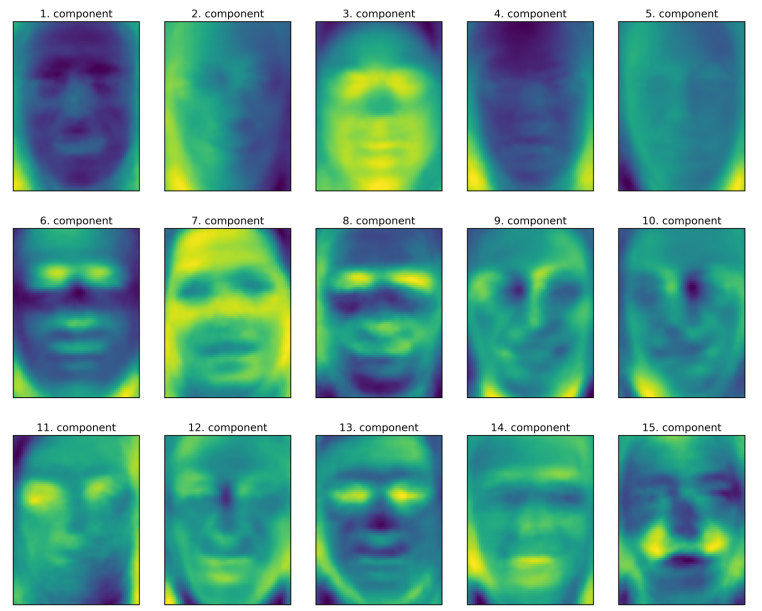
\includegraphics[scale=0.84]{../Imagen_Machine/PrimerPar}
	\caption{Vectores de componentes de las primeras 15 componentes principales de la data de caras}
	\label{PrimerPar}
\end{figure}

Volvamos al caso específico de PCA, aunque, introdujimos la transformación de PCA como rotanción   
de la data y luego dejando fuera las  componentes con baja varianza. Otra interpretación útil es tratar   de encontrar algunos números (los nuevos valores de característica después de la rotación PCA) para  que podamos expresar los puntos de prueba como una suma ponderada de las componentes principales 
(véase la Figura \ref{SumaX3}).\\



\begin{figure}[h!]
	\centering
	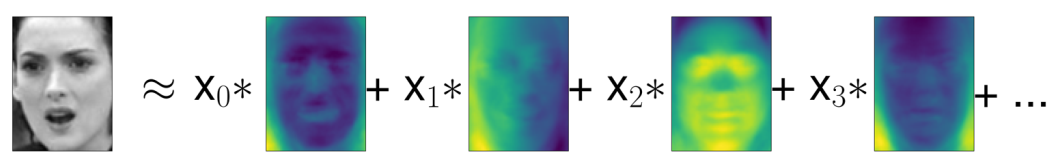
\includegraphics[scale=0.60]{../Imagen_Machine/SumaX3}
	\caption{Esquema del PCA como descomposición de una imagen en una suma ponderada de componentes}
	\label{SumaX3}
\end{figure}


Aquí, $x_{0}$,  $x_{1}$,  y así sucesivamente son los coeficientes de las componentes principales 
para esta data de puntos; en otras palabras, ellas son la representación de la imagen en el 
espacio rotado.\\


Otra forma para tratar de entender lo que un modelo de PCA está haciendo, es observar  las
reconstrucciones de la data original usando sólo algunos componentes.   
En la Figura \ref{CompontPric},  después de dejar fuera la segunda componente y llegar al tercer gráfico, deshacemos la rotación y añadimos la media  para obtener los nuevos puntos en el espacio original con la segunda  componente eliminada, como se muestra en el último gráfico. 

Podemos hacer una transformación similar para las caras, reduciendo los datos a sólo algunas componentes principales y luego  girando de nuevo en el espacio original. Este retorno al espacio de características 
original se puede hacer utilizando el método {\ttfamily inverse\_transform}.  Aquí, visualizamos la
reconstrucción de algunas caras usando 10, 50, 100, 500, ó 2000 componentes (Figura \ref{Reconstruc}):


\begin{lstlisting}  % [frame=single]	

In[32]: mglearn.plots.plot_pca_faces(X_train, X_test, image_shape)

\end{lstlisting} 


\begin{figure}[h!]
	\centering
	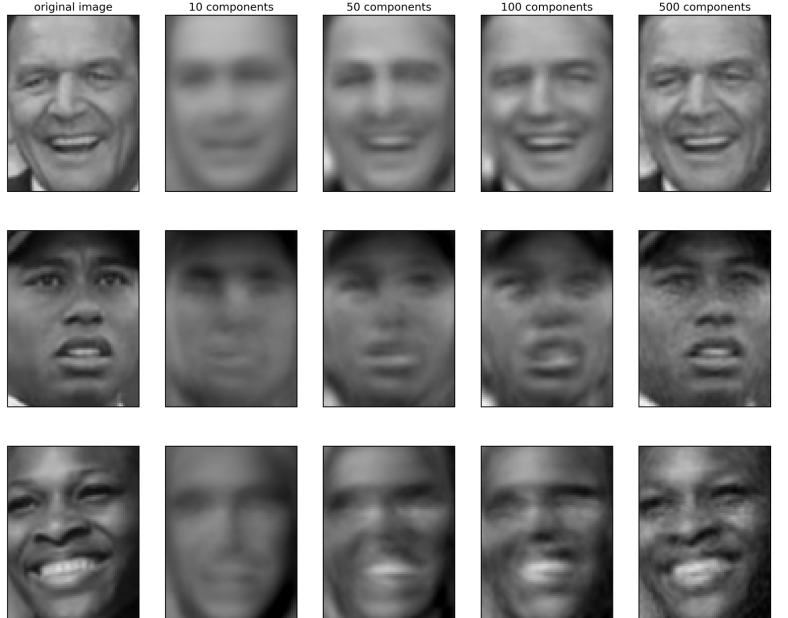
\includegraphics[scale=0.80]{../Imagen_Machine/Reconstruc}
	\caption{Reconstrucción de tres imágenes faciales utilizando un incremento del número  de componentes principales}
	\label{Reconstruc}
\end{figure}



Se puede ver que al utilizar  sólo las primeras 10 componentes principales, sólo la esencia de la imagen, como la orientación de la cara y la iluminación, se captura. Mediante el uso de más componentes principales, se capturan más detalles de la imagen. Esto corresponde al  incremento  de la sumatoria  de la figura \ref{SumaX3} para incluir más  términos. Usar tantas componentes como píxeles haya, significaría que no descartaríamos ninguna información después de la rotación, y reconstruiríamos la imagen perfectamente.\\ 

También podemos tratar de utilizar PCA para visualizar todas las caras del conjunto de datos en un diagrama de dispersión usando los dos primeros componentes principales (Figura \ref{Scatter2}), con clases dadas por quién se muestra en la imagen, de manera similar a lo que hicimos con la data cáncer:\\


\begin{lstlisting} 

In[33]: mglearn.discrete_scatter(X_train_pca[:, 0], X_train_pca[:, 1], y_train)
        plt.xlabel("First principal component")
        plt.ylabel("Second principal component")

\end{lstlisting} 


\begin{figure}[h!]
	\centering
	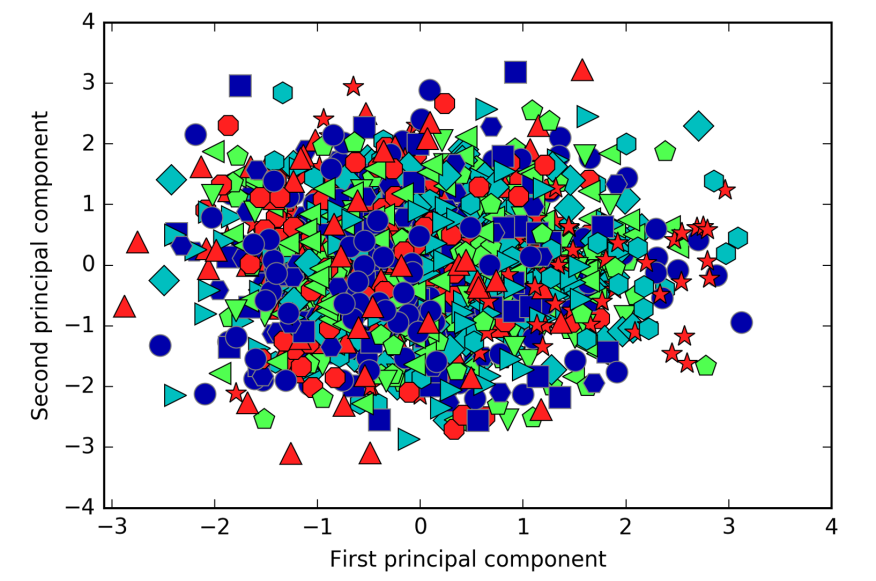
\includegraphics[scale=0.55]{../Imagen_Machine/Scatter2}
	\caption{Diagrama de dispersión del conjunto de datos de caras utilizando las dos primeras componentes principales (véase la figura \ref{Com2Pric} para la imagen correspondiente a la data de cáncer)}
	\label{Scatter2}
\end{figure}


Como se puede ver, cuando utilizamos sólo las dos primeras componentes principales de la totalidad de los datos es sólo una gran mancha, sin separación de clases visibles. Esto no es muy sorprendente, dado que incluso con 10 componentes, como se muestra en la Figura \ref{Reconstruc}, el PCA sólo captura las características muy toscas o bruscas de las caras.



\vspace{-2cm}	
\hspace{-1cm}
{\fcolorbox{red}{white}{ 		
		\begin{minipage}[16cm]{13.5cm}    %   centrado, largo y ancho                {14cm} 
			\vspace{0.4cm}	
			
			
			\begin{center}
				{\bf{Eigenface}}
			\end{center}	
			
			Un Eigenface (Wikipedia) es el nombre dado a un conjunto de vectores propios \index{vectores propios|seealso{eigenface}} cuando se utiliza en la visión por ordenador problema de humano de reconocimiento facial . [1] El enfoque de usar caras propias para el reconocimiento fue desarrollado por Sirovich y Kirby (1987) y utilizado por Matthew Turk y Alex Pentland en la clasificación de rostros. [2] Los vectores propios se derivan de la matriz de covarianza de la distribución de probabilidadsobre el espacio vectorial de alta dimensión de imágenes faciales. Las propias caras propias forman un conjunto base de todas las imágenes utilizadas para construir la matriz de covarianza. Esto produce una reducción de dimensión al permitir que el conjunto más pequeño de imágenes base represente las imágenes de entrenamiento originales. La clasificación se puede lograr comparando cómo las caras están representadas por el 
			conjunto base.	 \\		
			
		\end{minipage} 		
}}  \\



\subsection{Factorización matricial no negativa (NMF)} 


La factorización matricial no negativa es otro algoritmo de aprendizaje no supervisado que pretende
 extraer características útiles. Funciona de manera similar a PCA y también puede ser utilizado para la reducción de dimensionalidad. Como en PCA,  tratamos de escribir cada punto de datos como una suma ponderada de algunos componentes, como se ilustra en la Figura \ref{SumaX3}.   Pero mientras en PCA se quiere que las componentes sean ortogonales y que expliquen la mayor variación posible de los datos, en el NMF, se quiere que las componentes y los coeficientes no sean no negativos; es decir, queremos que tanto los componentes como los coeficientes sean mayores o iguales a cero. Por consiguiente, este método sólo puede aplicarse a datos en  que todas las característica son  no  negativa, ya que una suma no negativa de componentes no negativos no puede convertirse en no negativa. \\



El proceso de descomponer la data  en una suma ponderada no negativa es particularmente útil para los 
datos que se crean como la adición (o superposición de capas) de varias fuentes independientes, como una pista de audio de varias personas hablando, o música con muchos instrumentos. 

En estas situaciones, el NMF puede identificar los componentes originales que hacen la combinación de los datos. En general, el NMF da lugar a componentes más interpretables que el PCA, ya que los componentes y coeficientes negativos pueden provocar efectos de cancelación difíciles de interpretar.\\

Los caracteres o caras  propias  (eigenfaces\index{caras  propias}) en la Figura \ref{PrimerPar}, por ejemplo, contienen partes positivas y negativas, y como hemos mencionado en la descripción de PCA, el signo es en realidad arbitrario. Antes de aplicar NMF a la data de cara, vamos a revisar brevemente los datos sintéticos.


\subsubsection{Aplicar NMF a la data sintética}


A diferencia de lo que ocurre cuando se usa PCA, necesitamos  asegurar que la data sean  positivos para que el NMF tenga capacidad de funcionar con los datos. Esto significa que dónde se encuentran los datos en relación con el origen (0, 0) es realmente importante para NMF.  

Por lo tanto,  puede pensar en los componentes no negativos que se extraen como direcciones de (0, 0) hacia los datos. El siguiente ejemplo (Figura \ref{NMF1}) muestra los resultados del NMF en la data bidimensional de Toy:

\begin{lstlisting}  	
 
In[34]: mglearn.plots.plot_nmf_illustration()
 
\end{lstlisting} 


\begin{figure}[h!]
	\centering
	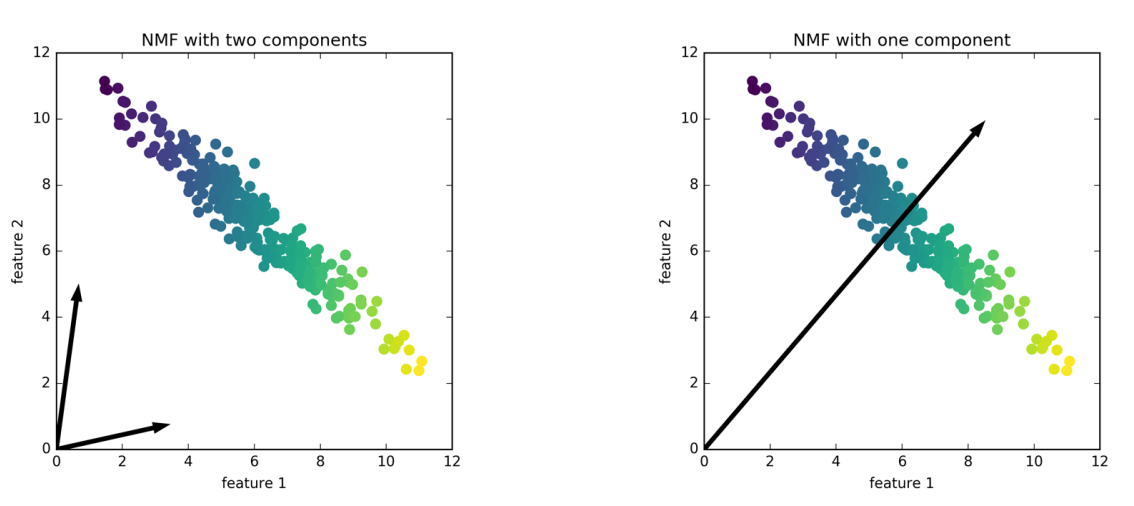
\includegraphics[scale=0.55]{../Imagen_Machine/NMF1}
	\caption{Componentes encontrados por la factorización matricial no negativa con dos componentes (izquierda) y una componente (derecha)}
	\label{NMF1}
\end{figure}


Para la  NMF con dos componentes, como se muestra a la izquierda de la figura \ref{NMF1}, está claro que todos los puntos en la data se pueden escribir como una combinación positiva de las dos componentes. Si hay
suficientes componentes para reconstruir perfectamente los datos (tantos componentes como  características haya), el algoritmo elegirá direcciones que apunten hacia los extremos de los datos.\\


Si sólo usamos una única  componente, la NMF crea una componente que apunta hacia la media, ya que apuntar en esa dirección explica mejor la data.  Puedes ver que en contraste con PCA, reducir el número de componentes no sólo elimina algunas direcciones, sino que crea ¡Un conjunto de componentes completamente diferente!  Las componentes en NMF tampoco están ordenadas de manera específica, por lo que no hay una  "{}primer componente no negativa{}":  todas  las componentes juegan por igual.  \\



NMF utiliza una inicialización aleatoria, lo que puede conducir a resultados diferentes
 dependiendo de  la semilla aleatoria.  En casos relativamente simples, como los datos sintéticos
  con dos componentes, donde toda la data pueden ser explicarse perfectamente, la aleatoriedad tiene poco efecto (aunque podría cambiar el orden o la escala de los componentes). En situaciones más complejas, puede haber cambios  drásticos.


\subsubsection{Aplicando NMF a imágenes de caras}


Ahora, aplicamos  NMF   a las  caras ctiquetadas  de data  Wild,   que usamos antes. El parámetro principal de NMF es el número de componentes a extraer. Por lo general, esto es menor que el número de características de entrada (de lo contrario, los datos podrían explicar cada píxel un componente separado).\\ 

Primero, inspeccionemos cómo el número de componentes impacta  y qué tan bien los datos pueden ser reconstruidos usando NMF (Figura \ref{NMF2}):


\begin{lstlisting} 

In[35]: mglearn.plots.plot_nmf_faces(X_train, X_test, image_shape)

\end{lstlisting} 



\begin{figure}[h!]
	\centering
	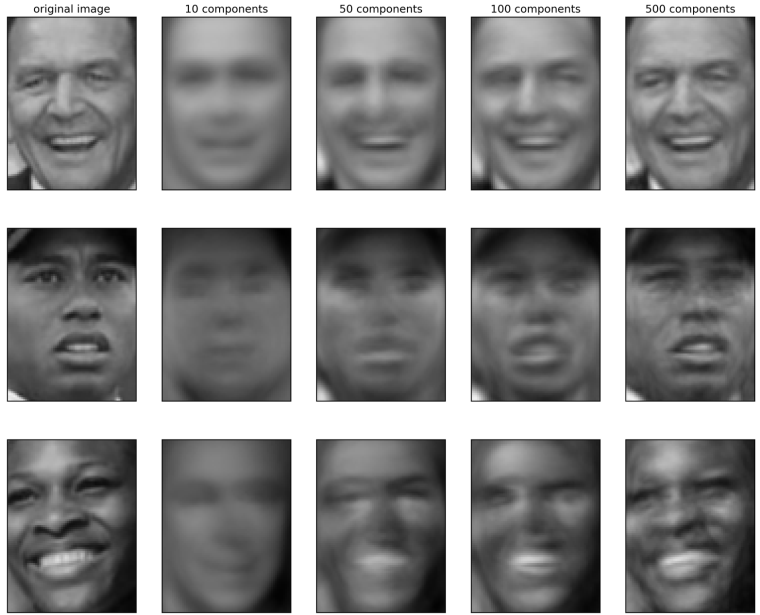
\includegraphics[scale=0.81]{../Imagen_Machine/NMF2}
	\caption{Reconstrucción de tres imágenes faciales utilizando un número creciente de componentes encontrados por NMF}
	\label{NMF2}
\end{figure}


Nuevamente la calidad de los datos transformados es similar al método  PCA, pero ligeramente 
baja la calidad. Esto es lo  esperado, ya que PCA encuentra las direcciones óptimas en términos de reconstrucción. Mientras que  NMF  no lo utiliza por su capacidad para reconstruir o codificar datos, sino para encontrar patrones interesantes dentro de los datos.

Como una primera vista   a los datos, intentemos extraer sólo unos pocos componentes (por ejemplo, 15).
La Figura \ref{NMF3} muestra el resultado:

\begin{lstlisting} 

In[36]: from sklearn.decomposition import NMF
        nmf = NMF(n_components=15, random_state=0)
        nmf.fit(X_train)
        X_train_nmf = nmf.transform(X_train)
        X_test_nmf = nmf.transform(X_test)
   
        fix, axes = plt.subplots(3, 5, figsize=(15, 12),
                                  subplot_kw={'xticks': (), 'yticks': ()})
                            
        for i, (component, ax) in enumerate(zip(nmf.components_, 
                                                 axes.ravel())):
            ax.imshow(component.reshape(image_shape))
            ax.set_title("{}. component".format(i))

\end{lstlisting} 



\begin{figure}[h!]
	\centering
	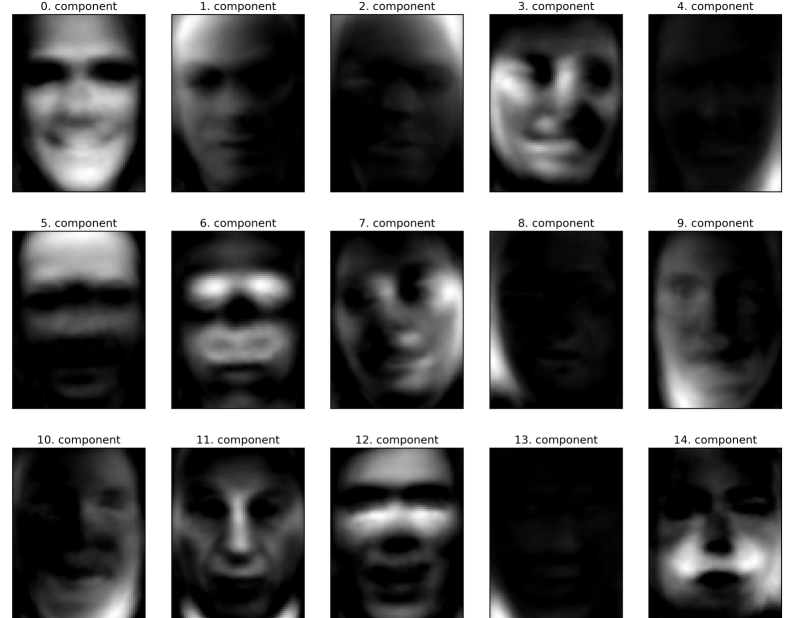
\includegraphics[scale=0.80]{../Imagen_Machine/NMF3}
	\caption{Las componentes encontrados por NMF en la data de caras al usar 15 componentes}
	\label{NMF3}
\end{figure}


Estas componentes son todas positivas, y así se asemejan a prototipos de caras mucho más que las componentes mostrados para PCA en la Figura \ref{PrimerPar}. Por ejemplo, se puede ver claramente que la componente 3 muestra una cara rotada un poco hacia la derecha, mientras que el componente 7 muestra una cara rotada un poco hacia la izquierda. Veamos las imágenes para las que estos componentes son particularmente fuertes, mostradas en las Figuras \ref{NMF4} y \ref{NMF5}:

\begin{lstlisting} 

In[37]: compn = 3
        # sort by 3rd component, plot first 10 images
        inds = np.argsort(X_train_nmf[:, compn])[::-1]
        fig, axes = plt.subplots(2, 5, figsize=(15, 8),
                                 subplot_kw={'xticks': (), 'yticks': ()})
        for i, (ind, ax) in enumerate(zip(inds, axes.ravel())):
            ax.imshow(X_train[ind].reshape(image_shape))

        compn = 7
        # sort by 7th component, plot first 10 images
        inds = np.argsort(X_train_nmf[:, compn])[::-1]
        fig, axes = plt.subplots(2, 5, figsize=(15, 8),
                                 subplot_kw={'xticks': (), 'yticks': ()})
        for i, (ind, ax) in enumerate(zip(inds, axes.ravel())):
            ax.imshow(X_train[ind].reshape(image_shape))


\end{lstlisting} 

%  np.argsor:   elemento más pequeño está en el índice 2, el siguiente más pequeño


\begin{figure}[h!]
	\centering
	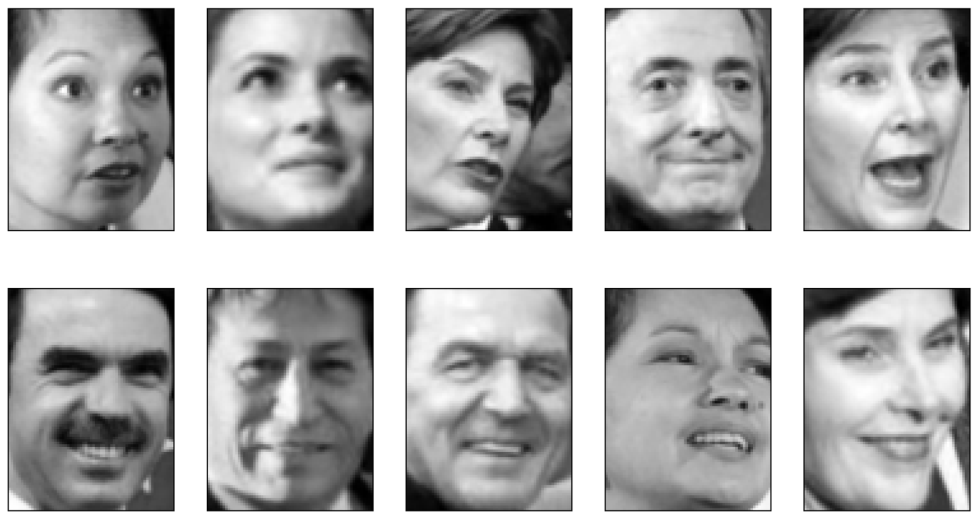
\includegraphics[scale=0.62]{../Imagen_Machine/NMF4}
	\caption{Caras que tienen un alto coeficiente para el componente 3}
	\label{NMF4}
\end{figure}




\begin{figure}[h!]
	\centering
	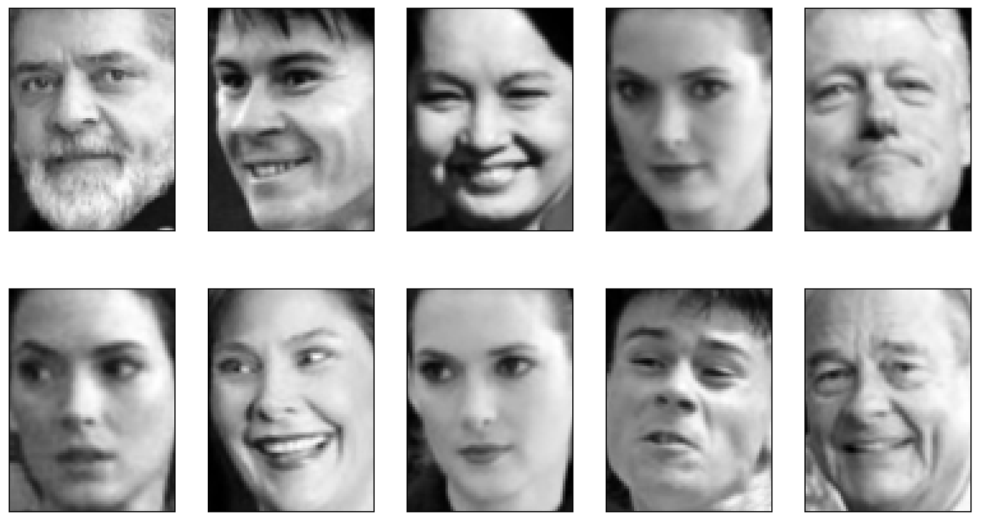
\includegraphics[scale=0.62]{../Imagen_Machine/NMF5}
	\caption{Caras que tienen un alto coeficiente para el componente 7}
	\label{NMF5}
\end{figure}




Como era de esperar, las caras que tienen un alto coeficiente para la componente 3 son caras que miran a la derecha (Figura \ref{NMF4}), mientras que las caras con un alto coeficiente para la componente 7 miran a la izquierda (Figura \ref{NMF5}). Como se mencionó anteriormente, la extracción de patrones como estos, funciona mejor para los datos con estructura aditiva, incluyendo audio, expresión génica\footnote{\scriptsize	{Expresión génica es el proceso mediante el cual la información codificada en un gen se utiliza para dirigir el montaje de una molécula de proteína. La célula lee la secuencia del gen en grupos de tres bases. Cada uno de estos grupos de tres bases (codón) corresponde a uno de los 20 aminoácidos diferentes usados para construir las proteínas.}}, y datos de texto. Veamos un ejemplo de datos sintéticos para ver cómo podría verse esto. \\

Digamos que estamos interesados en una señal que es una combinación de tres fuentes diferentes (Figura \ref{OriginalSenal}):


\begin{lstlisting} 

In[38]: S = mglearn.datasets.make_signals()
        plt.figure(figsize=(6, 1))
        plt.plot(S, '-')
        plt.xlabel("Time")
        plt.ylabel("Signal")

\end{lstlisting} 




\begin{figure}[h!]
	\centering
	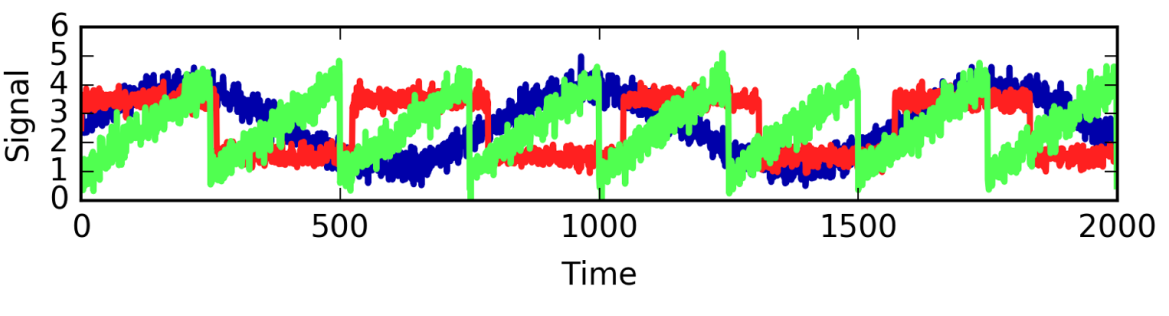
\includegraphics[scale=0.50]{../Imagen_Machine/OriginalSenal}
	\caption{Fuentes de señales originales}
	\label{OriginalSenal}
\end{figure}

%  OriginalSenal


Lamentablemente, no podemos observar las señales originales,  sólo una mezcla aditiva de
las tres. Queremos recuperar la descomposición de la señal mixta en las Componentes originales. Asumimos  que hay muchas formas diferentes de observar la mezcla (digamos 100 dispositivos de medición), cada uno de los cuales nos proporciona una serie de mediciones:\\


\begin{lstlisting}  

In[39]: # mix data into a 100-dimensional state
        A = np.random.RandomState(0).uniform(size=(100, 3))
        X = np.dot(S, A.T)
       print("Shape of measurements: {}".format(X.shape))

Out[39]:
    
    Shape of measurements: (2000, 100)

\end{lstlisting} 


Podemos usar NMF para recuperar las tres señales:


\begin{lstlisting}  

In[40]: nmf = NMF(n_components=3, random_state=42)
        S_ = nmf.fit_transform(X)
        print("Recovered signal shape: {}".format(S_.shape))

Out[40]:

    Recovered signal shape: (2000, 3)
    
\end{lstlisting} 


A modo de comparación, también aplicamos PCA:\\

\begin{lstlisting} 

In[41]: pca = PCA(n_components=3)
        H = pca.fit_transform(X)
	
\end{lstlisting} 


En la Figura \ref{NMFyCOMP} se muestra la actividad de la señal descubierta por NMF y PCA:\\

\begin{lstlisting}  

In[42]: models = [X, S, S_, H]
        names = ['Observations (first three measurements)',
                 'True sources',
                 'NMF recovered signals',
                 'PCA recovered signals']
            
        fig, axes = plt.subplots(4, figsize=(8, 4), 
                                 gridspec_kw={'hspace': .5},
                                 subplot_kw={'xticks': (), 'yticks': ()})
                            
        for model, name, ax in zip(models, names, axes):
            ax.set_title(name)
            ax.plot(model[:, :3], '-')

\end{lstlisting} 



\begin{figure}[h!]
	\centering
	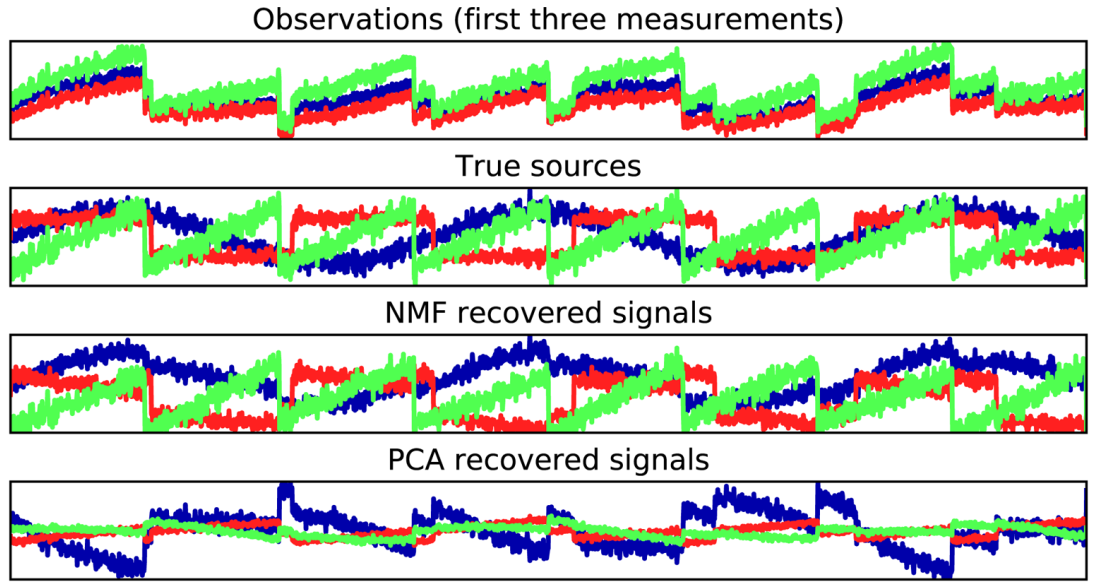
\includegraphics[scale=0.50]{../Imagen_Machine/NMFyCOMP}
	\caption{Recuperando fuentes mixtas usando NMF y PCA}
	\label{NMFyCOMP}
\end{figure}



La figura incluye 3 de las 100 mediciones de X como referencia. Como puedes ver,
NMF hizo un trabajo razonable al descubrir las fuentes originales, mientras que PCA falló y
usó la primera componente para explicar la mayoría de la variación en los datos.

 Es importante tener en cuenta que las componentes producidos por NMF no tienen un orden natural; en este ejemplo, el orden de las componentes de NMF es el mismo que en la señal original (vea el sombreado de las tres curvas), pero esto es puramente accidental.


Hay muchos otros algoritmos que pueden usarse para descomponer cada punto de la data en
una suma ponderada basasa en un conjunto fijo de componentes, como lo hacen PCA y NMF.  Analizar más algoritmos de este tipo están más allá del alcance de este libro;  además, las restricciones impuestas a
componentes y coeficientes generalmente involucra  la teoría de la probabilidad.  Pero si Usted está interesado en este tipo de extracción de patrones, le recomendamos revisar las secciones en la guía del usuario de {\ttfamily scikit\_learn} sobre análisis de componentes independientes (ICA), análisis factorial (FA) y  codificación sparse (diccionario de aprendizaje), generalmente en esta página puede encontrar casi todo lo referente a  \href{https://scikit-learn.org/stable/modules/decomposition.html}{\color{vino} métodos de descomposición}.  


\subsection{Aprendizaje múltiple con t-SNE}


Mientras que el PCA es con frecuencia  la  primera aproximación  buena  de la transformación de los  datos para visualizarlo usando un diagrama de dispersión, la naturaleza del método (aplicando 
rotación y luego descartando direcciones) límita su utilidad, como vimos con el gráfico de dispersión
de las caras etiquetadas en la data Wild.

Hay una clase de algoritmos para visualización llamado  algoritmos de múltiple aprendizaje (manifold learning algorithms)  que permiten mapeos mucho más complejos,  y a menudo proporciona mejor visualización. Uno de estos algoritmos  particularmente muy útil es el  algoritmo llamado   incrustación de vecinos estocásticos distribuidos en t, mejor conocido como t-SNE (t-distributed stochastic neighbor embedding).

%  incrustación de vecinos estocásticos distribuidos (t-SNE)  incrustación del vecino estocástica con distribuición t

Los algoritmos de aprendizaje múltiple están dirigidos principalmente a la visualización, por lo que rara vez se emplean para generar más de dos  nuevas características. Algunos de ellos, incluido t-SNE, 
cálculan una nueva representación de los datos de entrenamiento, pero no permiten transformaciones de nuevos
datos. Esto significa que estos algoritmos no se pueden aplicar a un conjunto de prueba;  
más bien, sólo pueden transformar los datos para los que fueron entrenados.  El aprendizaje múltiple puede ser útil para el análisis exploratorio de datos, pero rara vez se utiliza cuando el objetivo final es el aprendizaje supervisado. La idea detrás de t-SNE es encontrar una representación bidimensional de los datos que preservan las distancias entre los puntos lo mejor posible. 
 
t-SNE comienza con una representación bidimensional aleatoria para cada punto de la data, y luego trata de tomar los puntos que están más cerca, y los  que están más lejos en el espacio de característica original.  t-SNE pone más énfasis en los puntos cercanos, en lugar de preservar distancias entre puntos distantes. En otras palabras, trata de preservar la información que indica qué puntos son vecinos entre sí.\\


Aplicaremos  el  algoritmo  múltiple  de  aprendizaje t-SNE en la  dataset de dígitos escritos 
a mano (manuscrita) incluida en  {\ttfamily scikit-learn}. Cada punto de esta  dataset
es una imagen de 8x8 a escala de grises de un dígito escrito a mano entre 0 y 9.
 
  La Figura \ref{EscritoMano}  muestra una imagen del ejemplo  para cada clase:\\




\begin{lstlisting}  % [frame=single]	

In[43]: from sklearn.datasets import load_digits
        digits = load_digits()
   
        fig, axes = plt.subplots(2, 5, figsize=(10, 5),
                                subplot_kw={'xticks':(), 'yticks': ()})
        for ax, img in zip(axes.ravel(), digits.images):
            ax.imshow(img)


\end{lstlisting} 



\begin{figure}[h!]
	\centering
	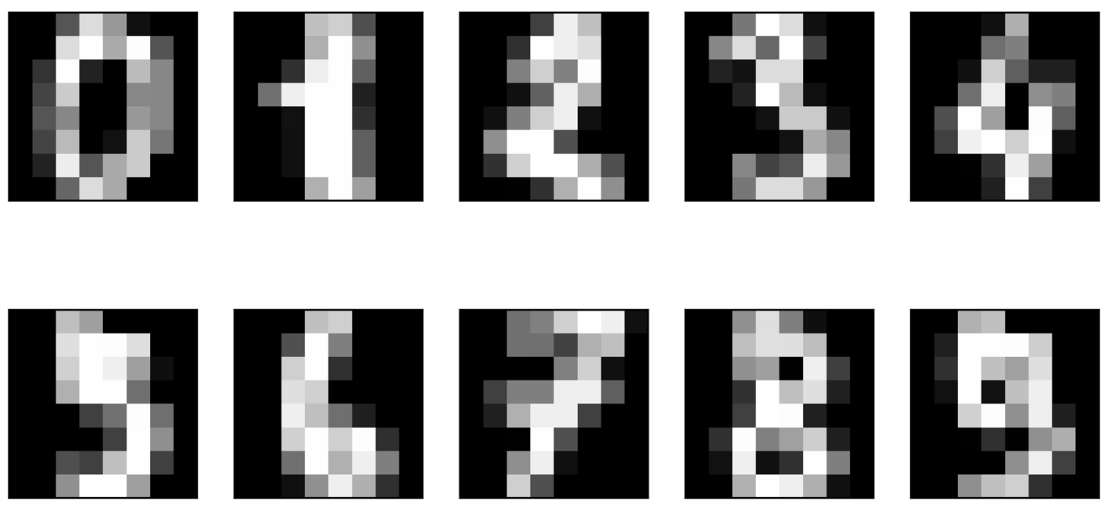
\includegraphics[scale=0.50]{../Imagen_Machine/EscritoMano}
	\caption{Ejemplo de imágenes de la data  de dígitos}
	\label{EscritoMano}
\end{figure}



Usemos PCA para visualizar los datos reducidos a dos dimensiones. Graficamos las dos primeras
componentes principales, y colorea cada punto por su clase (ver Figura \ref{Scatter3}):




\begin{lstlisting}  % [frame=single]	


In[44]: # build a PCA model
        pca = PCA(n_components=2)
        pca.fit(digits.data)
        # transform the digits data onto the first two principal components
        digits_pca = pca.transform(digits.data)
        colors = ["#476A2A", "#7851B8", "#BD3430", "#4A2D4E", "#875525",
                  "#A83683", "#4E655E", "#853541", "#3A3120", "#535D8E"]
        plt.figure(figsize=(10, 10))
        plt.xlim(digits_pca[:, 0].min(), digits_pca[:, 0].max())
        plt.ylim(digits_pca[:, 1].min(), digits_pca[:, 1].max())
        for i in range(len(digits.data)):
            # actually plot the digits as text instead of using scatter
            plt.text(digits_pca[i, 0], digits_pca[i, 1], 
                     str(digits.target[i]), color = colors[digits.target[i]],
                     fontdict={'weight': 'bold', 'size': 9})
        plt.xlabel("First principal component")
        plt.ylabel("Second principal component")


\end{lstlisting} 


Aquí, en realidad usamos las verdaderas clases de dígitos como glifos\footnote{\scriptsize	{glifo es atribuido a formas de escritura de las civilizaciones antiguas como los olmecas, mayas, xochilcas, aztecas, egipcios, entre otros}.}, para mostrar a qué clase pertenece. Los dígitos cero, seis, y cuatro están relativamente bien separados usando las dos primeras componentes principales, aunque todavía se superponen (solapan). La mayoría de los otros dígitos se superponen significativamente.


\begin{figure}[h!]
	\centering
	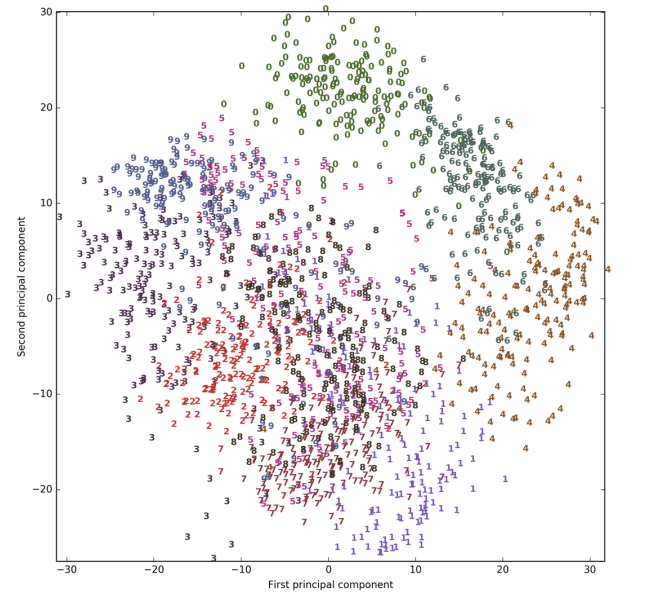
\includegraphics[scale=0.75]{../Imagen_Machine/Scatter3}
	\caption{Diagrama de dispersión del conjunto de datos de dígitos usando las dos primeras componentes principales}
	\label{Scatter3}
\end{figure}


Apliquemos t-SNE a la misma data y comparemos los resultados. Como t-SNE no admite la transformación de nuevos datos, la clase TSNE no tiene ningún método de transformación. En su lugar, podemos llamar al método  {\ttfamily fit\_transform}, que construirá el modelo y devolverá inmediatamente los datos transformados (ver Figura \ref{EscritoMano2}):\\



\begin{lstlisting}  % [frame=single]	

In[45]: from sklearn.manifold import TSNE
        tsne = TSNE(random_state=42)
        # use fit_transform instead of fit, as TSNE has no transform method
        digits_tsne = tsne.fit_transform(digits.data)

In[46]: plt.figure(figsize=(10, 10))
        plt.xlim(digits_tsne[:, 0].min(), digits_tsne[:, 0].max() + 1)
        plt.ylim(digits_tsne[:, 1].min(), digits_tsne[:, 1].max() + 1)
   
        for i in range(len(digits.data)):
            # actually plot the digits as text instead of using scatter
            plt.text(digits_tsne[i, 0], digits_tsne[i, 1], str(digits.target[i]),
                     color = colors[digits.target[i]],
                     fontdict={'weight': 'bold', 'size': 9})
        plt.xlabel("t-SNE feature 0")
        plt.xlabel("t-SNE feature 1")

\end{lstlisting} 



\begin{figure}[h!]                       
	\centering
	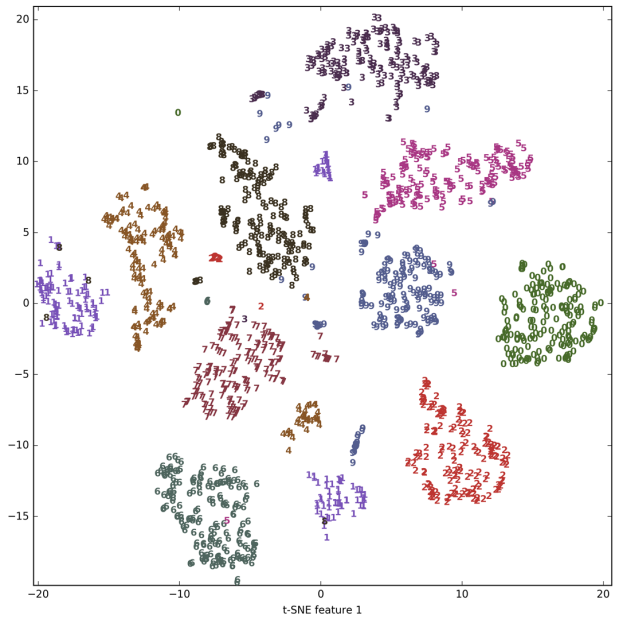
\includegraphics[scale=0.75]{../Imagen_Machine/EscritoMano2}
	\caption{Diagrama de dispersión del conjunto de datos de dígitos usando dos componentes encontrados por t-SNE}
	\label{EscritoMano2}
\end{figure}


El resultado de t-SNE es bastante notable. Todas las clases están claramente separadas.
Los unos y los nueve están algo divididos, pero la mayoría de las clases forman un sólo 
grupo denso.   Tenga en cuenta que este método no tiene conocimiento de las etiquetas de clase: es 
 no supervisado completamente. Aún así, puede encontrar una representación de los datos en dos dimensiones
que separa claramente las clases, basándose únicamente en qué tan cercanos están los puntos en el
espacio  original.

El algoritmo t-SNE tiene algunos parámetros de ajuste, aunque a menudo funciona bien con
la configuración predeterminada. Puedes intentar jugar con  {\ttfamily perplejidad} y {\ttfamily early\_exaggeration}, pero los efectos suelen ser menores.

\section{Clustering o Agrupación}



Como describimos anteriormente, la tarea del  clustering de dividir la dataset en grupos,
estos son llamados clústers, grupos o conglomerados.  El objetivo del  clustering  es dividir los datos de tal manera que los puntos dentro de un  grupo sean muy similares y los puntos entre grupos sean  muy diferentes.  De manera similar a los algoritmos de clasificación, estos  algoritmos  asignan (o predicen) un número a cada dato, que indica a qué grupo pertenece ese punto en particular.




\subsection{Agrupación de k-medias (k-Means Clustering)}

La agrupación de k-means es uno de los algoritmos de agrupación más simples y más utilizados.
 Intenta encontrar centros de clúster que sean representativos de ciertas regiones de la
data.  El algoritmo alterna entre dos pasos: asignar cada punto de la data al
centro de clúster más cercano y luego establece cada centro de clúster como la media de los 
puntos de datos  asignados. El algoritmo finaliza cuando la asignación de
las instancias a clústeres ya no cambian.

 El siguiente ejemplo (Figura \ref{k-media2}) illustra el algoritmo sobre la data sintética:\\

 

\begin{lstlisting}  % [frame=single]

In[47]: mglearn.plots.plot_kmeans_algorithm()
   
\end{lstlisting} 



\begin{figure}[h!]
	\centering
	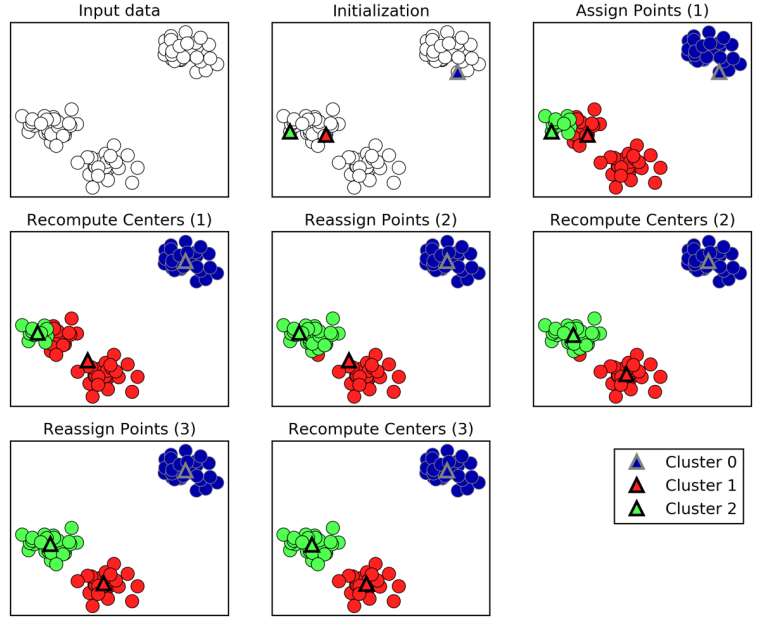
\includegraphics[scale=0.84]{../Imagen_Machine/k-media2}
	\caption{Datos de entrada y tres pasos del algoritmo k-means}
	\label{k-media2}
\end{figure}



Los centros de clúster se muestran como triángulos, mientras que los puntos de la data se muestran como círculos.  Los colores indican la etiqueta o membresía del clúster. Se configuró para buscar tres grupos, así que el algoritmo se inicializó declarando tres puntos de datos aleatoriamente como centro de clúster (ver "{}Inicialización"). Entonces comienza el algoritmo iterativo.  Primero, cada punto de datos es asignado al centro de clúster más cercano (consulte “Asignar puntos (1){}”).  Luego, el centro del clúster se actualizan para que sean la media de los puntos asignados (consulte "{}Centros de recálculo (1){}").  Luego, el proceso se repite dos veces más.  Después de la tercera iteración, la asignación de puntos a los centros de clúster se mantuvo sin cambios, por lo que el algoritmo se detiene.


Dados los nuevos puntos de datos, k-means asignará cada uno al centro de clúster más cercano. El siguiente
 ejemplo (Figura \ref{CentroKMedia}) muestra los límites de los centros de agrupación que se aprendieron
en la figura \ref{k-media2}:\\

\begin{lstlisting}  % [frame=single]	

In[48]: mglearn.plots.plot_kmeans_boundaries()

\end{lstlisting}


\begin{figure}[h!]
	\centering
	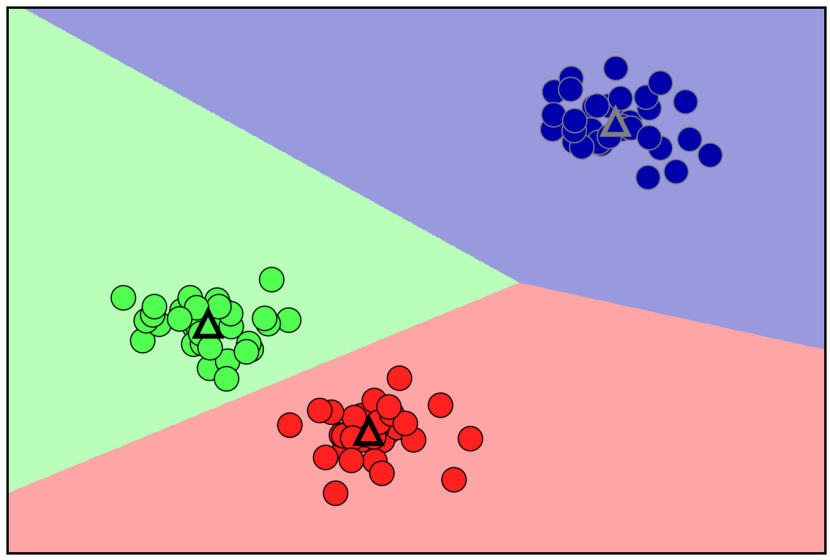
\includegraphics[scale=0.50]{../Imagen_Machine/CentroKMedia}
	\caption{Centros de clúster y límites de clúster encontrados por el algoritmo k-means}
	\label{CentroKMedia}
\end{figure}



 La aplicación de k-means con {\ttfamily scikit-learn} es bastante sencilla. Aquí, lo aplicamos 
 a la data  sintética utilizada en  gráficos anteriores.  Instanciamos la clase {\ttfamily KMeans}, y se configura  el número de clúster que nos interesa. Y llamamos el método {\ttfamily fit} sobre la data:\\

\begin{lstlisting}  % [frame=single]	

In[49]: from sklearn.datasets import make_blobs
        from sklearn.cluster import KMeans
   
        # generate synthetic two-dimensional data
        X, y = make_blobs(random_state=1)
   
        # build the clustering model
        kmeans = KMeans(n_clusters=3)
        kmeans.fit(X)

\end{lstlisting} 


El algoritmo le asigna  a cada punto del conjunto de entrenamiento en X  una etiqueta de cluster. Las  etiquetas se pueden encontrar en el atributo {\ttfamily kmeans.labels\_}:




\begin{lstlisting}  % [frame=single]	

In[50]: print("Cluster memberships:\n{}".format(kmeans.labels_))

Out[50]:

    Cluster memberships:
    [1 2 2 2 0 0 0 2 1 1 2 2 0 1 0 0 0 1 2 2 0 2 0 1 2 0 0 1 1 0 1 1 0 1 2 0 
     2 2 2 0 0 2 1 2 2 0 1 1 1 1 2 0 0 0 1 0 2 2 1 1 2 0 0 2 2 0 1 0 1 2 2 2 
     0 1 1 2 0 0 1 2 1 2 2 0 1 1 1 1 2 1 0 1 1 2 2 0 0 1 0 1]

\end{lstlisting}  % [frame=single]	



Como se configuro con tres clusters, estos  están numerados  como  0, 1  y  2. \\

También se le pueden asignar etiquetas de cluster a nuevos puntos, usando el método de {\ttfamily predict}. Cada nuevo punto es asignado al centro del clúster más cercano, pero el modelo existente no  cambia. Correr una {\ttfamily  predict} (predecición)   sobre la data de entrenamiento devuelve el mismo resultado que {\ttfamily labels\_}:


\begin{lstlisting}  % [frame=single]	


In[51]: print(kmeans.predict(X))

Out[51]:

    [1 2 2 2 0 0 0 2 1 1 2 2 0 1 0 0 0 1 2 2 0 2 0 1 2 0 0 1 1 0 1 1 0 1 2 0 
     2 2 2 0 0 2 1 2 2 0 1 1 1 1 2 0 0 0 1 0 2 2 1 1 2 0 0 2 2 0 1 0 1 2 2 2  
     0 1 1 2 0 0 1 2 1 2 2 0 1 1 1 1 2 1 0 1 1 2 2 0 0 1 0 1]

\end{lstlisting}  % [frame=single]	

Se puede ver que el clustering es algo similar a la clasificación, en  que cada item  obtiene
una etiqueta. Sin embargo, no existe una verdad fundamental,  y  en consecuencia, las etiquetas mismas
no tienen un significado a priori.   Volvamos al ejemplo de  clustering   con  las imágenes caras (faciales) que discutimos antes. Puede ser que el clúster 3 encontrado por el algoritmo contenga
sólo rostros (caras)  de la joven Bela. Aunque,  Usted sólo puedes saber  después de ver las fotos,   y además  el número 3 es arbitrario.  La única información que le brinda el algoritmo es que todas las caras etiquetadas como 3 son similares.\\


Para el agrupamiento que se calculó sobre la data bidimensional Toy, que significa que no debemos asignar ninguna importancia al hecho de que un grupo fue etiquetado 0 y otro fue etiquetado 1. Si corremos el algoritmo otra vez, podrían resultar en una numeración diferente para los grupos debido a la naturaleza aleatoria de la inicialización. En la  Figura \ref{Kmedia3clust} se presenta nuevamente estos datos en una  gráfica, los mismos grupos con etiquetas deferentes.


Los centros de clúster se almacenan en el atributo {\ttfamily cluster\_centers\_}, y en el  gráfico se muestran como triángulos:


\begin{lstlisting}  % [frame=single]	

In[52]: mglearn.discrete_scatter(X[:, 0], X[:, 1], kmeans.labels_,
                                  markers='o')
        mglearn.discrete_scatter(kmeans.cluster_centers_[:, 0],
                                 kmeans.cluster_centers_[:, 1], 
                                 [0, 1, 2], markers='^', markeredgewidth=2)


\end{lstlisting} 



\begin{figure}[h!]
	\centering
	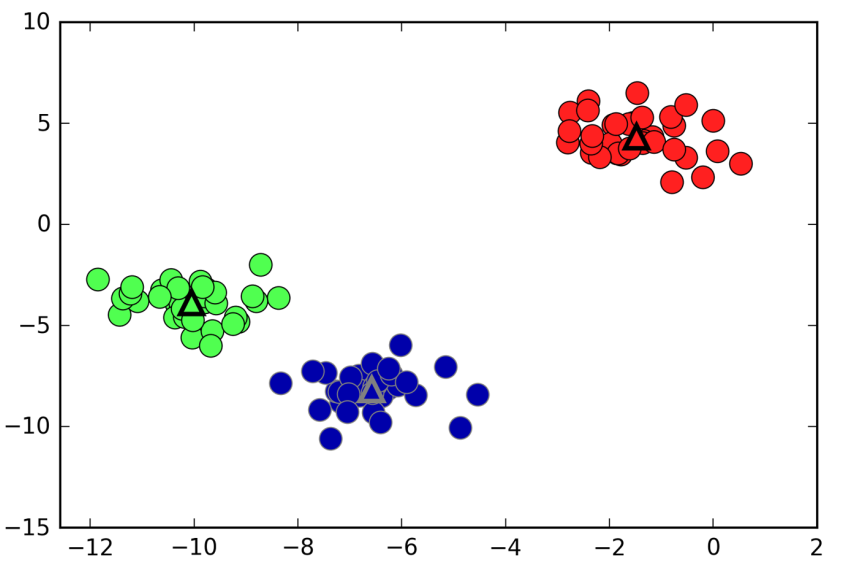
\includegraphics[scale=0.50]{../Imagen_Machine/Kmedia3clust}
	\caption{Asignaciones de clúster y centros de clúster encontrados por k-means con tres clusters}
	\label{Kmedia3clust}
\end{figure}


También podemos utilizar más o menos centros de cluster (Figura \ref{4kmedia}):


\begin{lstlisting}  % [frame=single]	

In[53]: fig, axes = plt.subplots(1, 2, figsize=(10, 5))
   
        # using two cluster centers:
        kmeans = KMeans(n_clusters=2)
        kmeans.fit(X)
        assignments = kmeans.labels_
   
        mglearn.discrete_scatter(X[:, 0], X[:, 1], assignments, ax=axes[0])
   
        # using five cluster centers:
        kmeans = KMeans(n_clusters=5)
        kmeans.fit(X)
        assignments = kmeans.labels_
   
        mglearn.discrete_scatter(X[:, 0], X[:, 1], assignments, ax=axes[1])


\end{lstlisting} 

%   conglomerados     grupos     clúster 

\begin{figure}[h!]
	\centering
	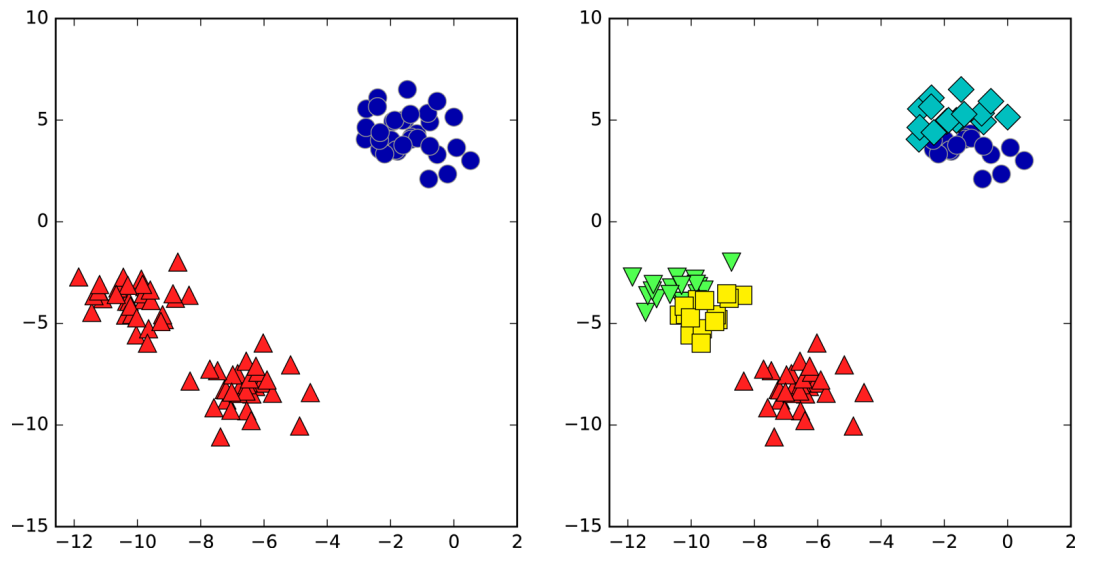
\includegraphics[scale=0.50]{../Imagen_Machine/4kmedia}
	\caption{Asignaciones de clúster  por k-means, dos  (en la izquierda) y cinco  (en la derecha)}
	\label{4kmedia}
\end{figure}


\subsubsection{Casos en que  falla de k-means}

 Incluso si conoce el número "{}correcto"{} de clusters para una dataset dada, k-means podría no siempre ser capaz de recuperarlos. Cada cluster es definido solamente por su centro, lo que significa que cada cluster es una forma convexa. Como resultado de esto, k-means sólo pueden cubrir formas relativamente simples. k-means también asume que todos los clusters  tienen el mismo "{}diámetro"{ }   en algún sentido; estos  siempre dibujan el límite entre clusters exactamente en el medio entre los centros de cluster.
 Esto puede llevar a veces a resultados sorprendentes, como se muestra en la Figura \ref{Sorprend}: 

 

\begin{lstlisting}  % [frame=single]

In[54]: X_varied, y_varied = make_blobs(n_samples=200,
                                        cluster_std=[1.0, 2.5, 0.5],
                                        random_state=170)
       y_pred = KMeans(n_clusters=3, random_state=0).fit_predict(X_varied)
  
       mglearn.discrete_scatter(X_varied[:, 0], X_varied[:, 1], y_pred)
       plt.legend(["cluster 0", "cluster 1", "cluster 2"], loc='best')
       plt.xlabel("Feature 0")
       plt.ylabel("Feature 1")
	

\end{lstlisting} 


	
	

\begin{figure}[h!]
	\centering
	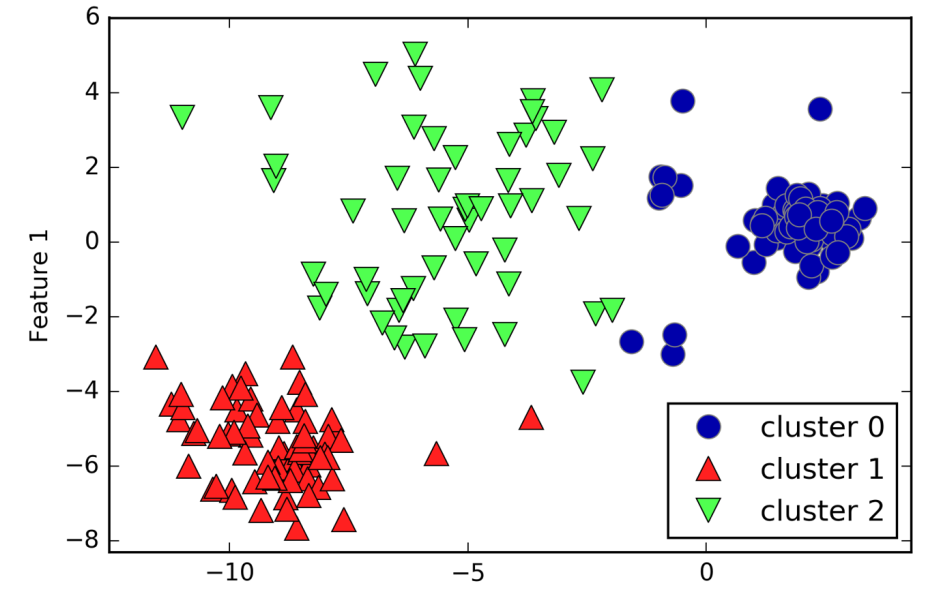
\includegraphics[scale=0.50]{../Imagen_Machine/Sorprend}
	\caption{Asignaciones de clúster encontradas por k-media cuando los clústers tienen densidades diferentes}
	\label{Sorprend}
\end{figure}


Podríamos  esperar  que la región densa de la izquierda inferior fuera el primer grupo, la región densa de la derecha superior fuera la segunda, y la región menos densa del centro  fuera la tercera. En cambio, tanto el cluster 0 como el cluster 1 tienen algunos puntos que están muy lejos de todos los otros puntos de estos clusters que se {}"{}alcanzan"{}  hacia el centro.  k-means también asume que todas las direcciones son igualmente importantes para cada cluster.  


El  gráfico (Figura \ref{KmediaFalla}) muestra el conjunto de datos bidimensionales donde hay tres partes claramente separadas en los datos. Sin embargo, estos grupos se estiran hacia la diagonal. Como k-means solo considera la distancia al centro del cluster más cercano, no puede manejar este tipo de datos: 

 

\begin{lstlisting}  % [frame=single]	

In[55]: # generate some random cluster data
        X, y = make_blobs(random_state=170, n_samples=600)
        rng = np.random.RandomState(74)
  
        # transform the data to be stretched
        transformation = rng.normal(size=(2, 2))
        X = np.dot(X, transformation)
  
        # cluster the data into three clusters
        kmeans = KMeans(n_clusters=3)
        kmeans.fit(X)
        y_pred = kmeans.predict(X)
   
        # plot the cluster assignments and cluster centers
        plt.scatter(X[:, 0], X[:, 1], c=y_pred, cmap=mglearn.cm3)
        plt.scatter(kmeans.cluster_centers_[:, 0], kmeans.cluster_centers_[:, 1],
                    marker='^', c=[0, 1, 2], s=100, linewidth=2, cmap=mglearn.cm3)
        plt.xlabel("Feature 0")
        plt.ylabel("Feature 1")


\end{lstlisting} 





Otro ejemplo donde k-means también funciona mal, se presenta cuando los clusters tienen formas más complejas, como los datos de {\ttfamily two\_moons}  analizados en el Capítulo \ref{Cap2} (ver Figura \ref{KmediaFalla2}):


\begin{lstlisting}  % [frame=single]	


In[56]: # generate synthetic two_moons data (with less noise this time)
        from sklearn.datasets import make_moons
        X, y = make_moons(n_samples=200, noise=0.05, random_state=0)
  
        # cluster the data into two clusters
        kmeans = KMeans(n_clusters=2)
        kmeans.fit(X)
        y_pred = kmeans.predict(X)
  
        # plot the cluster assignments and cluster centers
        plt.scatter(X[:, 0], X[:, 1], c=y_pred, cmap=mglearn.cm2, s=60)
        plt.scatter(kmeans.cluster_centers_[:, 0],
                    kmeans.cluster_centers_[:, 1], 
                    marker='^', c=[mglearn.cm2(0), mglearn.cm2(1)], 
                    s=100, linewidth=2)
        plt.xlabel("Feature 0")
        plt.ylabel("Feature 1")


\end{lstlisting}



\begin{figure}[!h!tbp]
	\begin{subfigure}[b]{0.5\textwidth}
		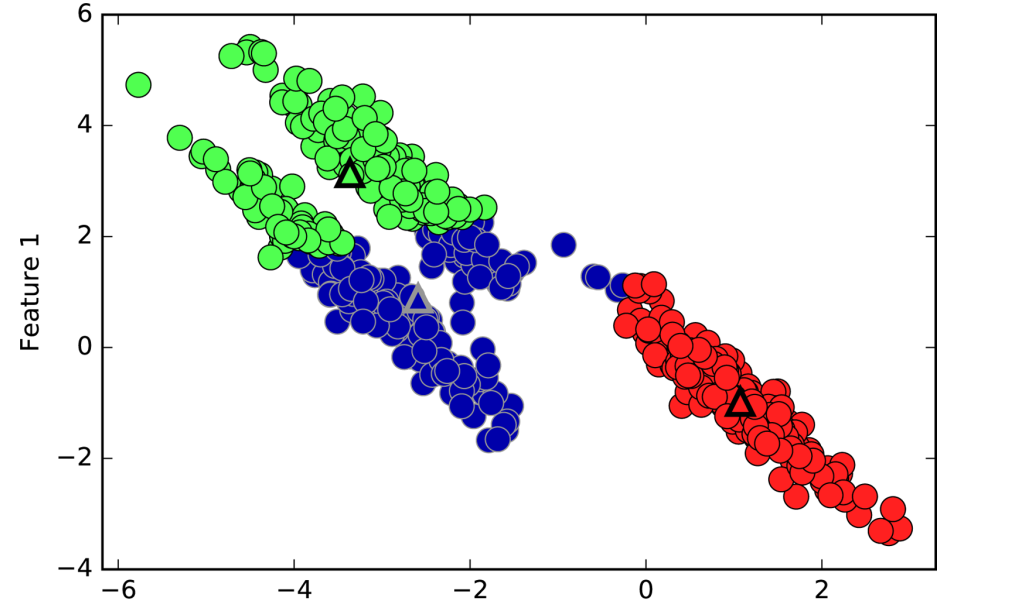
\includegraphics[width=7cm, height=5cm]{../Imagen_Machine/KmediaFalla}
		\caption{k-means no identifica los clústers \\no esféricos}
		\label{KmediaFalla}
		%	\caption{ }
		%	\label{  }
	\end{subfigure}
	\hfill
	\begin{subfigure}[b]{0.5\textwidth}
		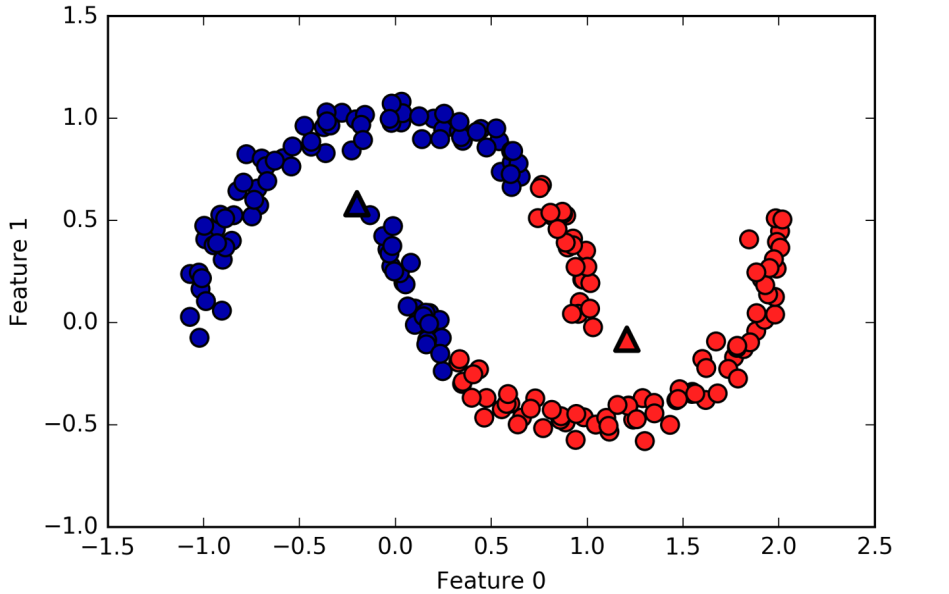
\includegraphics[width=7cm, height=5cm]{../Imagen_Machine/KmediaFalla2}
		\caption{k-means no identifica grupos con \\formas complejas}
		\label{KmediaFalla2}
	\end{subfigure}
	\caption{k-means sólo considera la distancia al centro del cluster más cercano, no puede manejar estos tipos de datos}
	%	\label{Grupo}
\end{figure}



 Aquí, podríamos esperar que el algoritmo de clustering pueda descubrir las dos formas de media luna. Sin embargo, esto no es posible usando el algoritmo k-means.






\subsubsection{Cuantificación vectorial}

 Ver el algoritmo  k-media como una  descomposición de la data es conocido como cuantificación vectorial{\footnote{\scriptsize{Cuantización vectorial, o ver k-medias como descomposición}}}.   A pesar de que k-media es un algoritmo de agrupamiento, hay paralelismos interesantes entre k-means y los métodos de descomposición como PCA y NMF que discutió antes. Puede recordar que PCA intenta encontrar direcciones de máxima varianza en los datos, mientras que NMF intenta encontrar componentes aditivos, que a menudo corresponden a  "{ }extremos{ }"{}  o  "{ }partes{ }"  { }de la data (ver Figura \ref{NMF1}).    Ambos métodos intentan expresar los puntos de la data como una suma de algunas componentes. Por otro lado, k-means intenta representar cada punto de la data  usando un centro de cluster.     Se podría considerar  que cada punto es representado por  una única componente, que en este caso sería dado por el centro del cluster. Esta visión de k-media es como un método de descomposición, donde cada punto se representa utilizando una sóla componente, es llamada cuantificación vectorial.


Veamos una comparación lado por lado  (side-by-side)  con  PCA, NMF, y k-media, mostrando las 
componentes  extraídas (Figura \ref{CompracionK1}), así como reconstrucciones de caras del conjunto de pruebas utilizando 100 componentes (Figura \ref{ComparacionK2}). Para k-means, la reconstrucción es el centro de cluster más cercano encontrado en el conjunto de entrenamiento: \\

\begin{lstlisting}  

In[57]: X_train, X_test, y_train, y_test = train_test_split(
            X_people, y_people, stratify=y_people, random_state=0)
        nmf = NMF(n_components=100, random_state=0)
        nmf.fit(X_train)
        pca = PCA(n_components=100, random_state=0)
        pca.fit(X_train)
        kmeans = KMeans(n_clusters=100, random_state=0)
        kmeans.fit(X_train)

        X_reconstructed_pca = pca.inverse_transform(pca.transform(X_test))
        X_reconstructed_kmeans = kmeans.cluster_centers_[kmeans.predict(X_test)]
        X_reconstructed_nmf = np.dot(nmf.transform(X_test), nmf.components_)

In[58]: fig, axes = plt.subplots(3, 5, figsize=(8, 8),
                                 subplot_kw={'xticks': (), 'yticks': ()})
        fig.suptitle("Extracted Components")
        for ax, comp_kmeans, comp_pca, comp_nmf in zip(
                axes.T, kmeans.cluster_centers_, pca.components_, 
                nmf.components_):
            ax[0].imshow(comp_kmeans.reshape(image_shape))
            ax[1].imshow(comp_pca.reshape(image_shape), cmap='viridis')
            ax[2].imshow(comp_nmf.reshape(image_shape))
      
        axes[0, 0].set_ylabel("kmeans")
        axes[1, 0].set_ylabel("pca")
        axes[2, 0].set_ylabel("nmf")

        fig, axes = plt.subplots(4, 5, 
                                 subplot_kw={'xticks': (), 'yticks': ()},
                                 figsize=(8, 8))
        fig.suptitle("Reconstructions")
        for ax, orig, rec_kmeans, rec_pca, rec_nmf in zip(
                axes.T, X_test, X_reconstructed_kmeans, X_reconstructed_pca,
                X_reconstructed_nmf):
       
            ax[0].imshow(orig.reshape(image_shape))
            ax[1].imshow(rec_kmeans.reshape(image_shape))
            ax[2].imshow(rec_pca.reshape(image_shape))
            ax[3].imshow(rec_nmf.reshape(image_shape))
   
        axes[0, 0].set_ylabel("original")
        axes[1, 0].set_ylabel("kmeans")
        axes[2, 0].set_ylabel("pca")
        axes[3, 0].set_ylabel("nmf")

\end{lstlisting} 


\begin{figure}[h!]
	\centering
	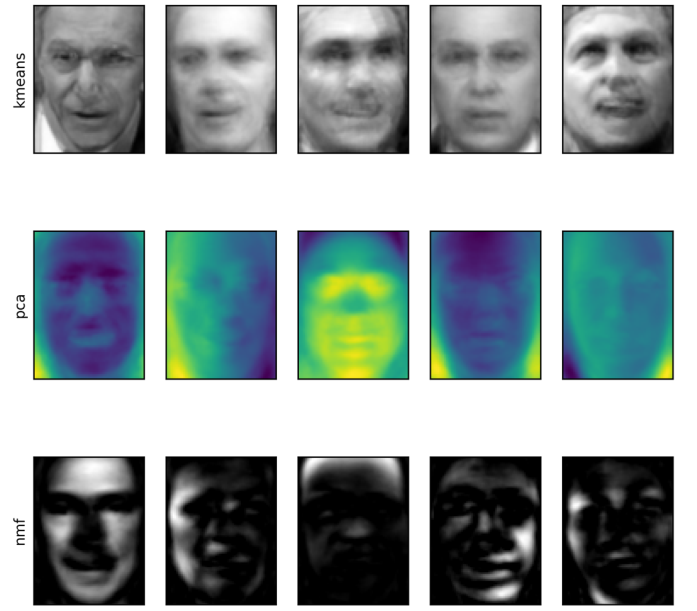
\includegraphics[scale=0.90]{../Imagen_Machine/CompracionK1}
	\caption{Comparación de los centros de conglomerados k-means con los componentes encontrados por PCA y NMF}
	\label{CompracionK1}
\end{figure}



\begin{figure}[h!]
	\centering
	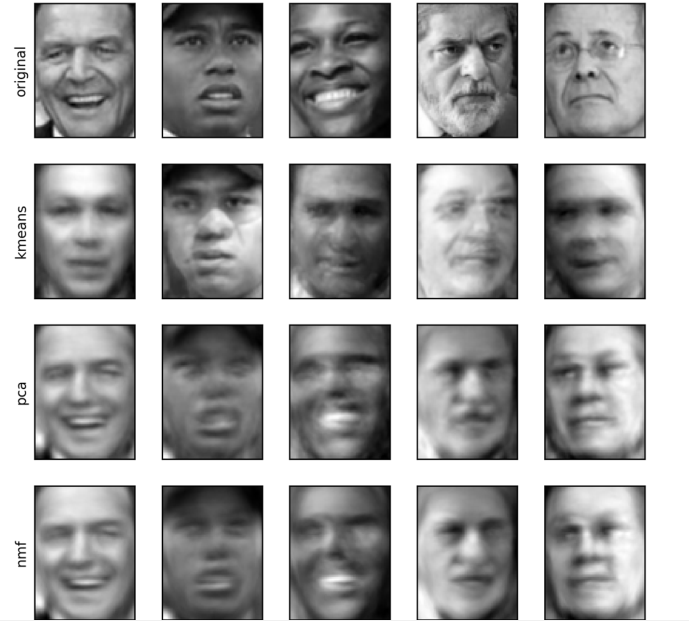
\includegraphics[scale=0.95]{../Imagen_Machine/ComparacionK2}
	\caption{Comparar reconstrucciones de imágenes usando k-means, PCA, y NMF con 100 componentes (ó centros de cluster: k-means usa  un centro de grupo por imagen)}
	\label{ComparacionK2}
\end{figure}

componentes (o centros de grupos): k-means usa solo un centro de grupo por imagen

Un aspecto interesante de la cuantificación vectorial usando k-medias es que podemos utilizar muchos más  clusters que dimensiones de entrada para codificar nuestros datos. 

Volvamos a los datos de {\ttfamily two\_moons}. Usando PCA o NMF, no hay mucho que podamos hacer a estos datos, ya que vienen en sólo dos dimensiones. Reducirlo a una dimensión con PCA o NMF destruiría completamente la estructura de los datos. Pero podemos encontrar una representación más expresiva con k-medias, usando más centros de  clusters (vea la Figura \ref{UsandoK}):







\begin{lstlisting}  % [frame=single]	

In[59]: X, y = make_moons(n_samples=200, noise=0.05, random_state=0)
   
        kmeans = KMeans(n_clusters=10, random_state=0)
        kmeans.fit(X)
        y_pred = kmeans.predict(X)
   
        plt.scatter(X[:, 0], X[:, 1], c=y_pred, s=60, cmap='Paired')
             plt.scatter(kmeans.cluster_centers_[:, 0], 
                         kmeans.cluster_centers_[:, 1], s=60, marker='^', 
                         c=range(kmeans.n_clusters), linewidth=2, cmap='Paired')
        plt.xlabel("Feature 0")
        plt.ylabel("Feature 1")
        print("Cluster memberships:\n{}".format(y_pred))

Out[59]:
    
   Cluster memberships:
   [9 2 5 4 2 7 9 6 9 6 1 0 2 6 1 9 3 0 3 1 7 6 8 6 8 5 2 7 5 8 9 8 6 5 3 7 0
    9 4 5 0 1 3 5 2 8 9 1 5 6 1 0 7 4 6 3 3 6 3 8 0 4 2 9 6 4 8 2 8 4 0 4 0 5
    6 4 5 9 3 0 7 8 0 7 5 8 9 8 0 7 3 9 7 1 7 2 2 0 4 5 6 7 8 9 4 5 4 1 2 3 1
    8 8 4 9 2 3 7 0 9 9 1 5 8 5 1 9 5 6 7 9 1 4 0 6 2 6 4 7 9 5 5 3 8 1 9 5 6
    3 5 0 2 9 3 0 8 6 0 3 3 5 6 3 2 0 2 3 0 2 6 3 4 4 1 5 6 7 1 1 3 2 4 7 2 7
    3 8 6 4 1 4 3 9 9 5 1 7 5 8 2]

\end{lstlisting} 



\begin{figure}[h!]
	\centering
	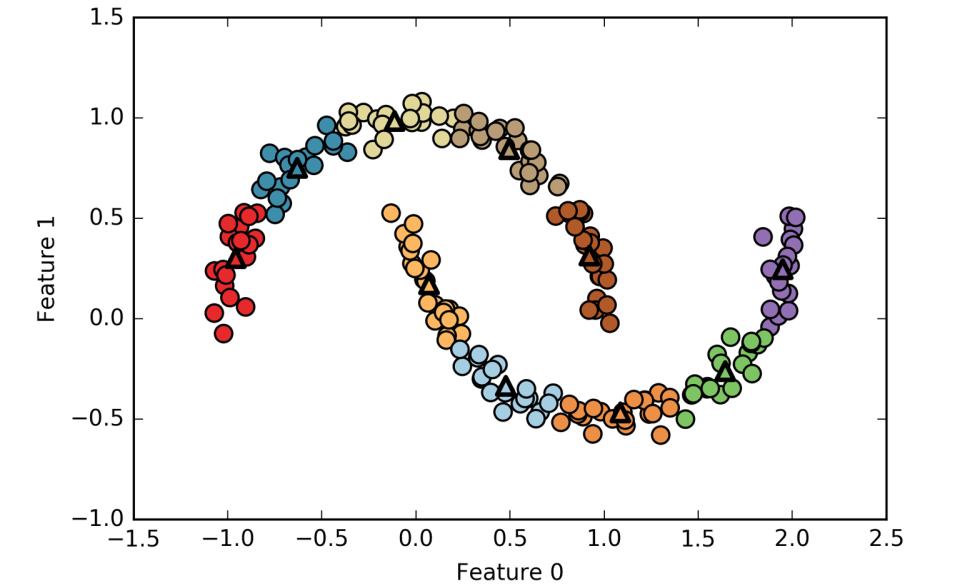
\includegraphics[scale=0.65]{../Imagen_Machine/UsandoK}
	\caption{Usando muchos clusters k-means para cubrir la variación en una data compleja}
	\label{UsandoK}
\end{figure}



Usando 10 centros de  cluster, significa que a cada punto se le asigna un número
entre 0 y 9. Podemos ver esto como si datos  se representaran usando 10 componentes
(es decir, tenemos 10  nuevas características),  y  todas las demás características a  0, aparte de la que representa el centro del clúster al que está asignado el punto. Usando  esta  nueva representación con 10 dimensiones, ahora sería posible separar las dos formas de  media luna   utilizando un modelo lineal, que no hubiera sido posible utilizando las dos características originales.   También es posible obtener una representación aún más expresiva de los datos mediante el uso de 
distancias a cada uno de los centros de clúster como características. Esto se puede lograr usando
el método {\ttfamily transform} de {\ttfamily kmeans} :



\begin{lstlisting}  % [frame=single]	



In[60]: distance_features = kmeans.transform(X)
        print("Distance feature shape: {}".format(distance_features.shape))
        print("Distance features:\n{}".format(distance_features))

Out[60]:
   
    Distance feature shape: (200, 10)
    Distance features:
    [[ 0.922  1.466  1.14 ...,  1.166  1.039  0.233]
     [ 1.142  2.517  0.12 ...,  0.707  2.204  0.983]
     [ 0.788  0.774  1.749 ..., 1.971  0.716  0.944]
     ...,
     [ 0.446  1.106  1.49 ...,  1.791  1.032  0.812]
     [ 1.39   0.798  1.981 ..., 1.978  0.239  1.058]
     [ 1.149  2.454  0.045 ..., 0.572  2.113  0.882]]



\end{lstlisting} 


k-means es un algoritmo muy popular para clustering, no solo porque es relativamente
fácil de entender e implementar, sino porque  también corre relativamente rápido.
 k-means  escala fácilmente  dataset grandes, y  {\ttfamily scikit-learn} incluso incluye una  variante 
  escalable  en la clase  {\ttfamily  MiniBatchKMeans}, que puede manejar dataset muy grandes.\\
  

Uno de los inconvenientes de k-means es que se basa en una inicialización aleatoria, que
significa que el resultado del algoritmo depende de una semilla aleatoria. Por defecto, {\ttfamily scikit-learn}  corre   el algoritmo 10 veces con 10 inicializaciones aleatorias diferentes, y
devuelve el mejor resultado.   
Otras desventajas de k-means son los supuestos   restrictivos de  k-means  sobre la forma de los grupos y el requisito de especificar el número  de grupos a buscar (aplicación que podría no ser conocido
en el mundo real).\\


A continuación, veremos dos algoritmos de agrupación, que mejoran esos inconvenientes en alguna forma.


\subsection{Clúster  Aglomerativo \\ (Agglomerative Clustering)}

El  Clúster  Aglomerativo o  agrupamiento aglomerativo se refiere a una colección de algoritmos de agrupamiento que todos se basan en los mismos principios: el algoritmo comienza declarando cada punto su propio clúster, y luego fusiona los dos clúster más similares hasta que algún criterio de parada se satisface.  El criterio de parada implementado en scikit-learn es el número de clusters, por lo que los clusters similares se fusionan hasta que sólo queda el número especificado de clusters. Hay varios criterios de vinculación que especifican exactamente cómo se mide el "{}clúster más similar"{}. Esta medida siempre se define entre dos clusters existentes. 

Las siguientes tres opciones se implementan en scikit-learn:\\



{\ttfamily Ward}

Es la opción por defecto, ward escoge los dos clústeres para fusionarlo de tal manera que la varianza dentro de todos los clústeres aumente lo menos posible. Esto a menudo conduce a grupos que son de tamaño similar.\\


{\ttfamily  Average}

El  Average  fusiona los dos clusters que tienen la distancia media más pequeña entre todos sus puntos.\\




{\ttfamily  Complete}

La opción  Complete (también conocido como enlace máximo) fusiona  dos clústeres que tienen la distancia máxima más pequeña entre sus puntos.\\




ward trabaja en la mayoría de los conjuntos de datos, y lo usaremos en nuestros ejemplos.  Si los clusters  un número muy diferente de elementos ( por ejemplo,  si uno es mucho más grande que todos los demás),  la opción  Average  o Complete podría funcionar mejor.\\



La siguiente gráfica (Figura 3-33) ilustra el  progreso del clúster aglomerativo sobre un conjunto de datos bidimensionales, buscando tres grupos:\\ 



\begin{lstlisting} 

In[61]: mglearn.plots.plot_agglomerative_algorithm()
   
\end{lstlisting} 




\begin{figure}[h!]
	\centering
	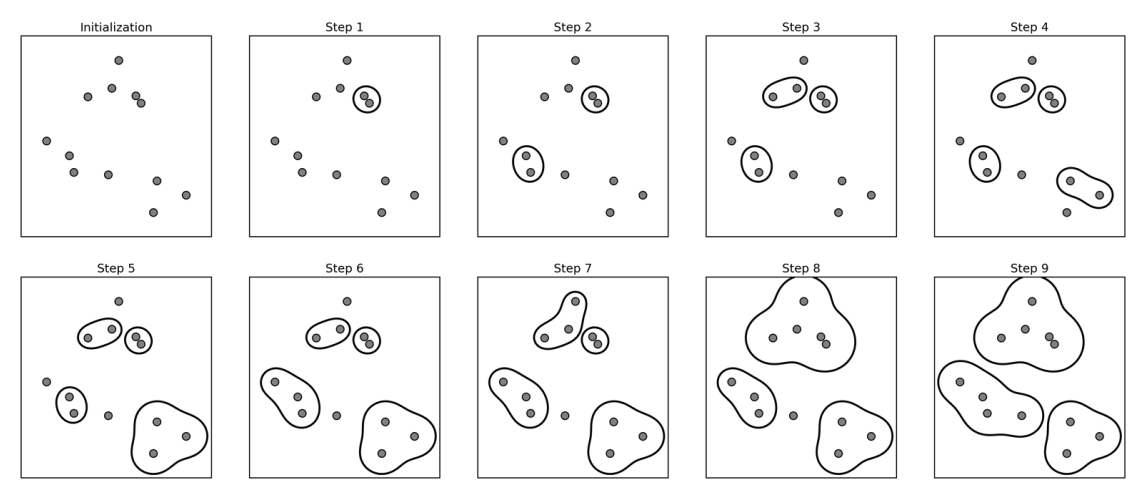
\includegraphics[scale=0.55]{../Imagen_Machine/Aglomerativo1}
	\caption{La agrupación de aglomeraciones se une iterativamente a los dos grupos más cercanos}
	\label{Aglomerativo1}
\end{figure}


Inicialmente, cada punto es su propio clúster. Luego, en cada paso, los dos clústeres más cercanos se fusionan. En los primeros cuatro pasos, se seleccionan dos clusters de un sólo punto que se unen en clusters de dos puntos. En el paso 5, uno de los clústeres de dos puntos se extiende a un tercer punto, y así sucesivamente. En el paso 9, sólo quedan tres clústeres. Como especificamos que estamos buscando tres grupos, el algoritmo se detiene. 

Veamos cómo funciona el clúster  Aglomerativo  con los  tres clústeres simples. Debido a la forma en que funciona el algoritmo, el  clúster  Aglomerativo no puede hacer predicciones para nuevos puntos de datos. 
Por lo tanto, el  clúster  Aglomerativo no tiene un método de predicción. Para construir el modelo y obtener clúster etiquetados en el conjunto de entrenamiento, se use el  método {\ttfamily fit\_predict}. El resultado se muestra en la figura \ref{Aglomerativo2}:\\
 
\begin{lstlisting}  % [frame=single]
 
In[62]: from sklearn.cluster import AgglomerativeClustering
        X, y = make_blobs(random_state=1)
   
        agg = AgglomerativeClustering(n_clusters=3)
        assignment = agg.fit_predict(X)
   
        mglearn.discrete_scatter(X[:, 0], X[:, 1], assignment)
        plt.xlabel("Feature 0")
        plt.ylabel("Feature 1")
   
\end{lstlisting} 

\begin{figure}[h!]
	\centering
	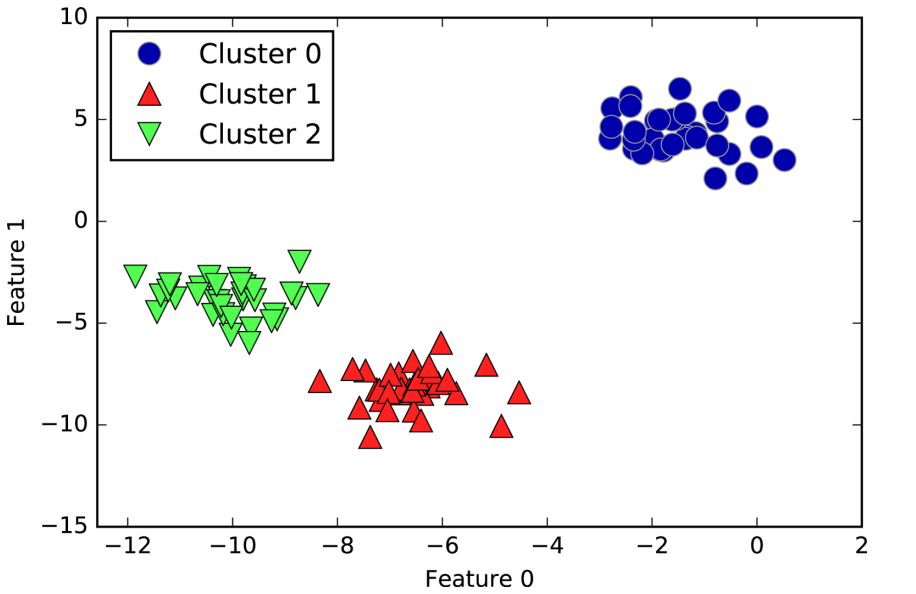
\includegraphics[scale=0.55]{../Imagen_Machine/Aglomerativo2}
	\caption{Asignación de clústeres utilizando clústeres aglomerativos con tres clústeres}
	\label{Aglomerativo2}
\end{figure}

	


Como se esperaba, el algoritmo recupera los clúster perfectamente. Mientras que el {\ttfamily scikit-learn} implementa clúster aglomerativo y  requiere que especifique el número de grupos que desea que encuentre el algoritmo, los métodos de clúster aglomerativo proporcionan una ayuda para elegir el número correcto, esta opción se discute a continuación.


\subsubsection{Clúster jerárquico y dendrogramas}


El clúster  Agglomerative produce lo que se conoce como clúster jerárquico. El 
clúster procede de forma iterativa, y cada punto hace un viaje desde  un clúster con un único
punto, hasta pertenecer a algún clúster final. Cada paso intermedio proporciona un
agrupación de los datos (con un número diferente de agrupaciones). A veces es útil
observar  todas las agrupaciones posibles conjuntamente. 

El siguiente ejemplo (Figura \ref{Jerarquico}) muestra una superposición de todos los posibles
 clusterings que se muestran en la Figura \ref{Aglomerativo1}, proporcionando alguna idea de cómo cada clúster se divide en grupos más pequeños:\\  

\begin{lstlisting}  % [frame=single]	

In[63]: mglearn.plots.plot_agglomerative()

\end{lstlisting} 



\begin{figure}[h!]
	\centering
	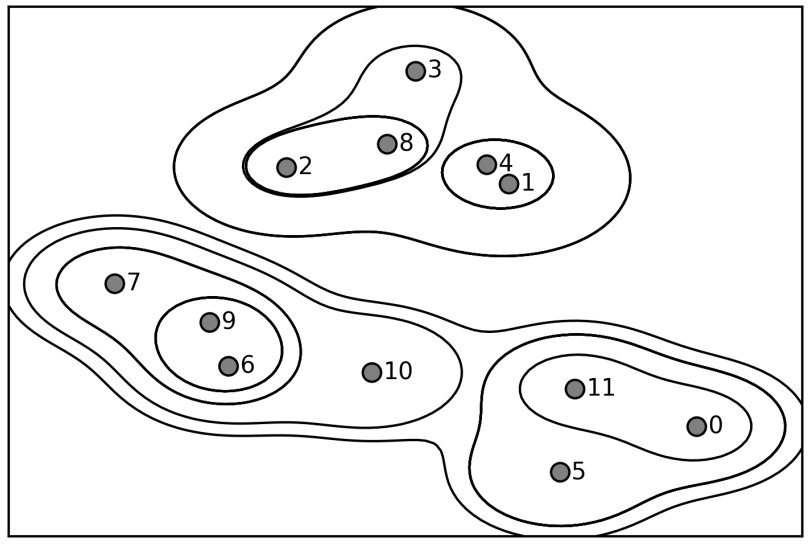
\includegraphics[scale=0.55]{../Imagen_Machine/Jerarquico}
	\caption{Asignación jerárquica en clústeres (mostrada como líneas) generada con el clúster Aglomerative, con los puntos   de la data   enumerandos (Figura \ref{Dendog}).}
	\label{Jerarquico}
	\end{figure}


Si bien esta visualización proporciona una visión muy detallada de la agrupación jerárquica, se basa en la naturaleza bidimensional de los datos,  y  por lo tanto, no se puede utilizar en conjuntos de datos que tienen más de dos características.  Sin embargo, hay otra herramienta para visualizar
agrupamiento jerárquico, llamado dendrograma, que puede manejar datas multidimensional.\\

Desafortunadamente, {\ttfamily scikit-learn} actualmente no tiene la funcionalidad para dibujar dendrogramas.   Sin embargo, puede generarlos fácilmente con {\ttfamily SciPy}. Los algoritmos de clúster {\ttfamily SciPy} tienen una interfaz ligeramente diferente al  algoritmo de clustering  de {\ttfamily scikit-learn}. {\ttfamily SciPy} proporciona una función que toma una matriz de datos $X$ y calcula una matriz  enlace, que codifica similitudes de clúster jerárquico.

Y se puede introducir esta matriz de enlaces en la función de dendrograma de Scipy para trazar el dendrograma, como se muestra a continuación (Figura \ref{Dendog}):\\


\begin{lstlisting}  % [frame=single]	

In[64]: # Import the dendrogram function and the ward clustering function 
        # from SciPy
        from scipy.cluster.hierarchy import dendrogram, ward
   
        X, y = make_blobs(random_state=0, n_samples=12)
        # Apply the ward clustering to the data array X
        # The SciPy ward function returns an array that specifies the 
        # distances
        # bridged when performing agglomerative clustering
        linkage_array = ward(X)

        # Now we plot the dendrogram for the linkage_array containing the
        #  distances
        # between clusters
        dendrogram(linkage_array)
   
        # Mark the cuts in the tree that signify two or three clusters   
        ax = plt.gca()
        bounds = ax.get_xbound()
        ax.plot(bounds, [7.25, 7.25], '--', c='k')
        ax.plot(bounds, [4, 4], '--', c='k')
   
        ax.text(bounds[1], 7.25, ' two clusters', va='center',
                fontdict={'size': 15})
        ax.text(bounds[1], 4, ' three clusters', va='center', 
                fontdict={'size': 15})
        plt.xlabel("Sample index")
        plt.ylabel("Cluster distance")

\end{lstlisting} 



\begin{figure}[h!]
	\centering
	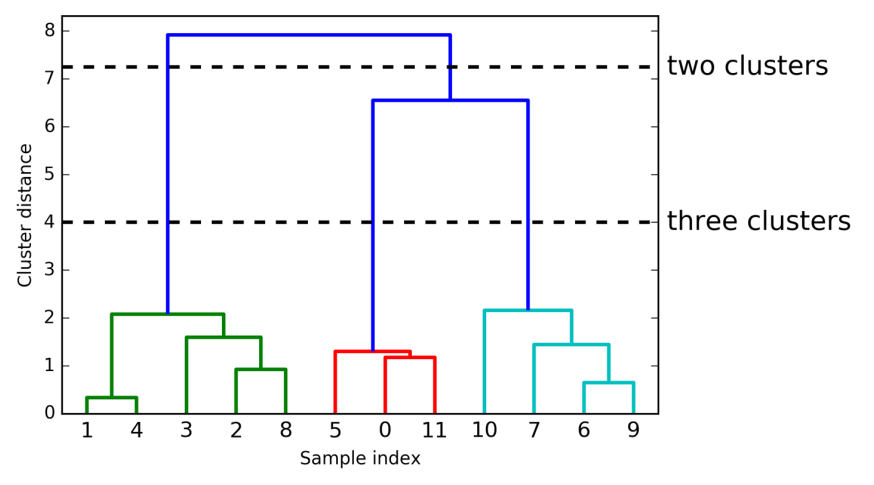
\includegraphics[scale=0.55]{../Imagen_Machine/Dendog}
	\caption{Dendrograma del clúster mostrado en la Figura \ref{Jerarquico} con líneas que indican divisiones en dos y tres grupos}
	\label{Dendog}
\end{figure}


El dendrograma muestra los puntos de datos como puntos en la parte inferior (numerados de 0 a 11). Luego, se grafica un árbol con estos puntos (representando clusters de un solo punto) como las hojas, y se añade un nuevo nodo padre para cada dos  clusters que se unen. Leyendo de abajo hacia arriba, los puntos de datos 1 y 4 se unen primero (como se puede ver en la Figura \ref{Aglomerativo1}).  A continuación, los puntos 6 y 9 se unen en un grupo, y así sucesivamente. En el nivel superior, hay dos ramas, una que consta de los puntos 11, 0, 5, 10, 7, 6 y 9, y la otra que consta de los puntos 1, 4, 3, 2 y 8.   Estos corresponden a los dos clústeres más grandes en el lado izquierdo del gráfico.\\


El eje $y$ del el dendrograma, no solo especifica cuándo en el algoritmo  Agglomerative  fusiona dos clústers, sino también la longitud de separación de los clusters fusionados  en cada nodo o rama. Las ramas más largas en este dendrograma son las tres líneas que están marcadas por la línea de los "{}tres grupos".{}  El hecho de que estas sean las ramas más largas, indica que pasar de tres a dos grupos significó fusionar algunos puntos muy distantes. Vemos esto de nuevo en la parte superior del gráfico, donde la fusión de los dos clúster restantes en un sólo clúster, se hace  con  puentes de una distancia relativamente grande. \\

Desafortunadamente, el clustering  Agglomerative  falla al intentar separar formas complejas como el conjunto de datos de {\ttfamily two\_moons}. Este inconveniente lo supera al algoritmo DBSCAN,  en la siguiente sección se describe este algoritmo. Sin embargo, tanto Agglomerative como DBSCAN, no permiten predicciones para nuevos  datos de prueba, pero se puede implementar  {\ttfamily fit\_predict} para la predicción.



\subsection{DBSCAN}  

Otro algoritmo clúster  muy usado  es DBSCAN, que significa   "{}agrupación espacial basada en densidad de aplicaciones con ruido"{}  ({}densitybased spatial clustering of applications with noise{}). Los principales beneficios de DBSCAN es que no requiere que el usuario establezca el número de clústeres a priori,   puede capturar clusteres  de formas complejas,  y pueden identificar puntos que no forman parte del cluster.  DBSCAN es algo más lento que el clustering agglomerative y k-means, pero puede escala dataset relativamente grandes.\\



DBSCAN funciona identificando puntos que se encuentran en regiones "{}abarrotadas{}"  {} en el 
espacio de caraterísticas, donde hay muchos puntos de datos  juntos. Estas regiones se conocen como
regiones densas en el espacio de características. La idea detrás de DBSCAN es que los clústeres que forman regiones densas de datos, estan  separadas por regiones que están relativamente vacías. \\
 
 Los puntos que se encuentran dentro de una región densa se denominan muestras  núcleos (muestras centrales) o puntos  núcleo.    El algoritmos tiene dos parámetro, un mínimo de muestras  {\ttfamily min\_samples}  y  una distancia  {\ttfamily eps}. Si  hay  al  menos  una cierta cantidad  puntos {\ttfamily min\_samples}   dentro de una distancia dada {\ttfamily eps} a un determinado  punto, ese punto  se clasifica como una muestra núcleo.     
Las muestras núcleos que se encuentran a menor distancia (entre sí) que  {\ttfamily eps}, son colocadas  en un  mismo clúster. \\

 El   algoritmo funciona seleccionando un punto arbitrario para comenzar. Luego encuentra todos los puntos que que están a menor o igual distancia {\ttfamily eps}   a ese punto. Si hay menos de  {\ttfamily min\_samples} puntos dentro de la distancia {\ttfamily eps}  del punto de partida, este punto es etiquetado como ruido, lo que significa que no pertenece a ningún clúster; si hay más de {\ttfamily min\_samples} puntos dentro  de una distancia de  {\ttfamily eps}, el punto es etiqueta como una muestra núcleo y se le asigna una nueva etiqueta de clúster. Luego,  todos los vecinos (dentro de  {\ttfamily eps}) del punto son visitados, si algunos de ellos  aún no han sido asignados a ningún grupo, se les asigna la nueva etiqueta del grupo que se acaba de crear. Si son muestras núcleo, sus vecinos son visitados por turnos, y así sucesivamente.  El  clúster  crece hasta que no haya más muestras  núcleo dentro de la distancia  {\ttfamily eps} del clúster. Luego se selecciona otro punto que aún no se ha visitado, y el mismo procedimiento es  repetido.\\



Al final, hay tres tipos de puntos: los puntos núcleos o centrales, los puntos que están dentro de distancia  {\ttfamily eps}   de los puntos núcleos (llamados puntos  límite o frontera), y los puntos ruido.     Cuando el algoritmo DBSCAN se ejecuta sobre una dataset particular varias veces, el clustering  de los puntos núcleos  siempre es el mismo, y los puntos que se etiquetarán como ruido también son los mismos. Sin embargo, un punto  límite  podría ser vecino de más  un clúster de muestra  núcleo.  Por lo tanto, la pertenencia al clúster de los puntos límite depende del orden en que se visiten los puntos.  Por lo general, sólo hay unos pocos puntos límite, y esta ligera dependencia del  orden no es importante.\\


A continuación se aplicar la ténica DBSCAN sobre la data sintética que utilizamos para ilustrar el clúster Agglomerative.  DBSCAN no permite predicciones sobre nuevos datos de prueba, por lo que utilizaremos el método {\ttfamily fit\_predict} para correr el clustering  y  devolver las etiquetas de clúster en un sólo paso:\\ 

\begin{lstlisting} 
In[65]: from sklearn.cluster import DBSCAN
        # Dataset Toy
        X, y = make_blobs(random_state=0, n_samples=12)  
   
        dbscan = DBSCAN()
        clusters = dbscan.fit_predict(X)
        print("Cluster memberships:\n{}".format(clusters))

Out[65]:
    
    Cluster memberships:
    [-1 -1 -1 -1 -1 -1 -1 -1 -1 -1 -1 -1]


\end{lstlisting}  % [frame=single]	



Como puede ver,  todos los puntos de la dataset   se les asignó la etiqueta -1,  lo que significa que son   ruido.  Esto es una consecuencia de la configuración de parámetros por defecto para  {\ttfamily eps} y
 {\ttfamily min\_samples}, que no están ajustados  para la dataset  pequeña de Toy. 

A continuación se  muestran Los clústers asignados  para diferentes valores de {\ttfamily min\_samples} y  {\ttfamily eps}, y se visualizan en la Figura \ref{DBSCAN1}:\\ 

\begin{lstlisting}  
In[66]: mglearn.plots.plot_dbscan()

Out[66]:
   
    min_samples: 2 eps: 1.000000 cluster: [-1 0 0 -1 0 -1 1 1 0 1 -1 -1]
    min_samples: 2 eps: 1.500000 cluster: [0 1 1 1 1 0 2 2 1 2 2 0]
    min_samples: 2 eps: 2.000000 cluster: [0 1 1 1 1 0 0 0 1 0 0 0]
    min_samples: 2 eps: 3.000000 cluster: [0 0 0 0 0 0 0 0 0 0 0 0]
    min_samples: 3 eps: 1.000000 cluster: [-1 0 0 -1 0 -1 1 1 0 1 -1 -1]
    min_samples: 3 eps: 1.500000 cluster: [0 1 1 1 1 0 2 2 1 2 2 0]
    min_samples: 3 eps: 2.000000 cluster: [0 1 1 1 1 0 0 0 1 0 0 0]
    min_samples: 3 eps: 3.000000 cluster: [0 0 0 0 0 0 0 0 0 0 0 0]
    min_samples: 5 eps: 1.000000 cluster: [-1 -1 -1 -1 -1 -1 -1 -1 -1 -1
                                           -1 -1]
    min_samples: 5 eps: 1.500000 cluster: [-1 0 0 0 0 -1 -1 -1 0 -1 -1 -1]
    min_samples: 5 eps: 2.000000 cluster: [-1 0 0 0 0 -1 -1 -1 0 -1 -1 -1]
    min_samples: 5 eps: 3.000000 cluster: [0 0 0 0 0 0 0 0 0 0 0 0]

\end{lstlisting} 


\begin{figure}[h!]
	\centering
	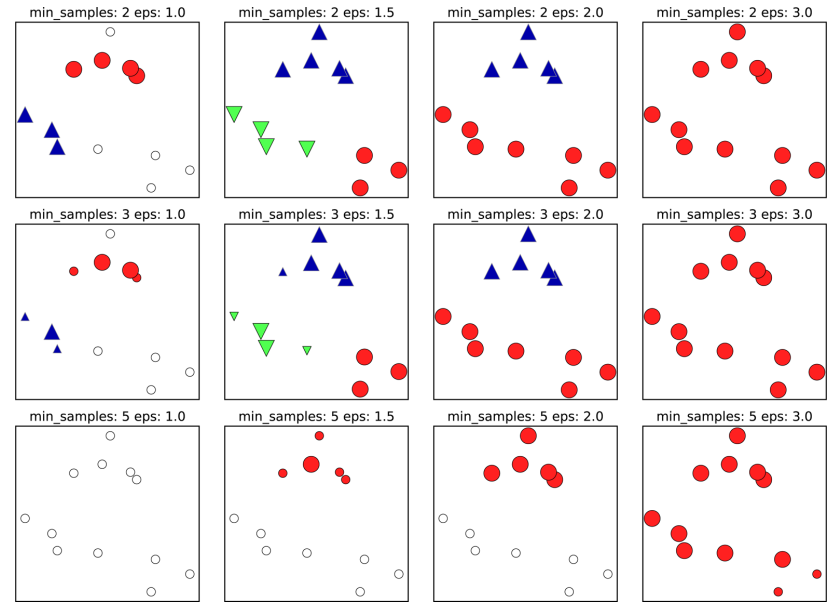
\includegraphics[scale=0.75]{../Imagen_Machine/DBSCAN1}
	\caption{Asignaciones de clúster encontradas por DBSCAN con ajustes variables 
		para los parámetros  {\ttfamily min\_samples}  y  {\ttfamily eps} }
	\label{DBSCAN1}
\end{figure}


En el  gráfico \ref{DBSCAN1}, los puntos que pertenecen a clusters son figuras sólidos, mientras que los puntos  ruido se muestran en blanco. Las muestras  núcleo se muestran como marcas grandes, mientras que los puntos de límite se muestran  como marcas más pequeñas.

El incremento de {\ttfamily eps} (de izquierda a derecha en la figura \ref{DBSCAN1}) significa que más puntos serán incluidos en un clúster. Esto hace que los clúster crezcan, pero también puede conducir a que varios clúster se unan en uno sólo. El aumento de {\ttfamily min\_samples} (de arriba a abajo en la figura \ref{DBSCAN1}) significa que menos puntos serán clasificados como puntos núcleos, y más puntos serán etiquetados como ruido.

El parámetro {\ttfamily eps} es  importante, ya que determina lo que significa estar   "{}cerca"{}  (algo como distancia). Configurar {\ttfamily eps} para que sea muy pequeño significará que no hay puntos como muestras  núcleos, y puede llevar a que todos los puntos se etiqueten como ruido, mientras que configurar {\ttfamily eps} para que sea muy grande dará como resultado que todos los puntos formen un único grupo.\\


La configuración  {\ttfamily min\_samples}  determina principalmente si los puntos en regiones menos densas
seran etiquetados como valores atípicos o como sus propios grupos.  Si disminuye {\ttfamily min\_samples}, cualquier cosa que hubiera sido un clúster con menos de {\ttfamily min\_samples}, muchas muestras ahora serán etiquetadas como ruido. El parámetro {\ttfamily min\_samples} determina el tamaño mínimo del grupo.   Esta situación puede verse claramente en la Figura \ref{DBSCAN1}, cuando el  {\ttfamily min\_samples}  va de 3  a  5  con {\ttfamily  eps} =1.5. En el caso de  {\ttfamily min\_samples}=3, hay tres grupos: uno de cuatro {\ttfamily min\_samples}, uno de cinco y uno de tres.  Usando {\ttfamily min\_samples}= 5, los dos clúster pequeños (con tres y cuatro puntos) ahora son etiquetados como ruido, y sólo un clúster con las cinco muestras restantes.\\
 

DBSCAN no requiere establecer el número de clústeres explícitamente, la configuración de {\ttfamily eps}
controla implícitamente cuántos grupos se encontrarán. Encontrar una buena configuración para {\ttfamily eps}   a veces es más fácil después de escalar los datos usando  {\ttfamily StandardScaler  o  MinMaxScaler},  pues el  uso de las técnicas para escalar la data garantizará que todas las características tengan rangos similares. \\

La Figura \ref{DBSCAN2} muestra el resultado de ejecutar DBSCAN sobre la  dataset {\ttfamily two\_moons}. El algoritmo realmente encuentra los dos semicírculos (half-circles) y los separa usando la configuración por defecto:


\begin{lstlisting}  % [frame=single]
	
In[67]: X, y = make_moons(n_samples=200, noise=0.05, random_state=0)
   
        # rescale the data to zero mean and unit variance
        scaler = StandardScaler()
        scaler.fit(X)
        X_scaled = scaler.transform(X)
   
        dbscan = DBSCAN()
        clusters = dbscan.fit_predict(X_scaled)
        # plot the cluster assignments
        plt.scatter(X_scaled[:, 0], X_scaled[:, 1], c=clusters,
                    cmap=mglearn.cm2, s=60)
        plt.xlabel("Feature 0")
        plt.ylabel("Feature 1")
   
\end{lstlisting} 



\begin{figure}[h!]
	\centering
	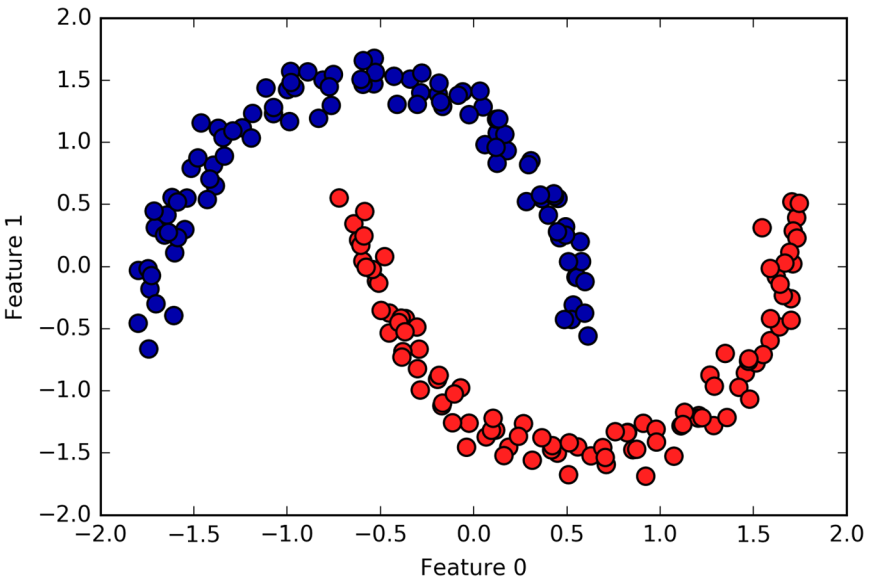
\includegraphics[scale=0.55]{../Imagen_Machine/DBSCAN2}
	\caption{Asignación de clúster encontrada por DBSCAN utilizando el valor predeterminado de {\ttfamily eps} = 0.5 }
	\label{DBSCAN2}
\end{figure}


El algoritmo produce el número deseado de clusters (en este caso dos), el conjunto de parámetros parece funcionar bien. Si disminuimos {\ttfamily eps} a 0.2 (el valor por defecto es 0.5), obtendremos ocho clusters,  claramente son demasiado. El aumento de {\ttfamily eps} a 0.7 resulta en un sólo clúster.\\

Al utilizar DBSCAN, es necesario ser cuidadoso con el manejo de las asignaciones de clúster que retorna. 
El uso de -1 para indicar ruido puede provocar efectos inesperados al usar las etiquetas del clúster  para indexar otra matriz.





\subsection{Comparando y evaluando los  algoritmos de Clúster}  

Uno de los desafíos en la aplicación de algoritmos de clustering es que es muy difícil evaluar
qué tan bien funcionó un algoritmo, y comparar los resultados entre diferentes algoritmos. Después de hablar de los algoritmos  k-means, agglomerative y DBSCAN, ahora podemos compararlo sobre algunas 
dataset  del mundo real.


\subsubsection{Evaluar los clustering con la verdad fundamental}



Hay métricas que se pueden utilizar para evaluar el resultado de un algoritmo de agrupamiento relativo a una verdad fundamental (clúster correcto)\index{verdad fundamental}, las más importantes son el índice de aleatoriedad ajustado (adjusted rand
index, ARI) y la información mutua normalizada (normalized mutual information, NMI),  ambos proporcionan una medida cuantitativa  entre 0 y 1. \\

Analicemos los algoritmos k-media, Agglomerative  y  DBSCAN  comparando los resultados con métrica ARI. También se incluye cómo se ve cuando asignamos puntos aleatoriamente a dos clusters para efecto de  comparar (ver Figura \ref{ComparDBSCAN}):\\
 
\begin{lstlisting}  	

In[68]: from sklearn.metrics.cluster import adjusted_rand_score
        X, y = make_moons(n_samples=200, noise=0.05, random_state=0)
   
        # rescale the data to zero mean and unit variance
        scaler = StandardScaler()
        scaler.fit(X)
        X_scaled = scaler.transform(X)
   
        fig, axes = plt.subplots(1, 4, figsize=(15, 3),
                                 subplot_kw={'xticks': (), 'yticks': ()})
  
        # make a list of algorithms to use
        algorithms = [KMeans(n_clusters=2), 
                      AgglomerativeClustering(n_clusters=2), DBSCAN()]
                 
        # create a random cluster assignment for reference
        random_state = np.random.RandomState(seed=0)
        random_clusters = random_state.randint(low=0, high=2, size=len(X))
  
        # plot random assignment
        axes[0].scatter(X_scaled[:, 0], X_scaled[:, 1], c=random_clusters,
                        cmap=mglearn.cm3, s=60)
        axes[0].set_title("Random assignment - ARI: {:.2f}".format(
                           adjusted_rand_score(y, random_clusters)))
           
        for ax, algorithm in zip(axes[1:], algorithms):
             # plot the cluster assignments and cluster centers
             clusters = algorithm.fit_predict(X_scaled)
             ax.scatter(X_scaled[:, 0], X_scaled[:, 1], c=clusters,
                       cmap=mglearn.cm3, s=60)
             ax.set_title("{} - ARI: {:.2f}".format(
                     algorithm.__class__.__name__, 
                     adjusted_rand_score(y, clusters)))

\end{lstlisting} 



\begin{figure}[h!]
	\centering
	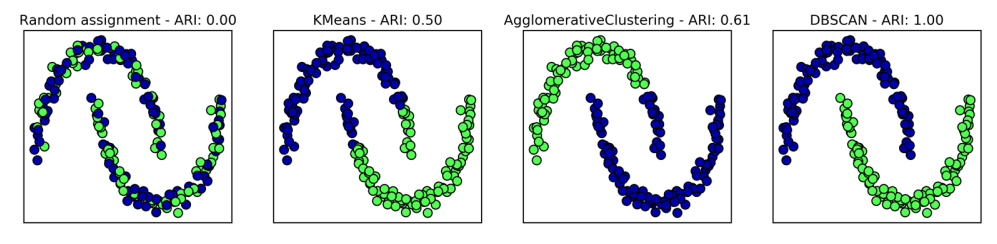
\includegraphics[scale=0.65]{../Imagen_Machine/ComparDBSCAN}
	\caption{Comparación de asignación aleatoria, k-media, Agglomerative  y  DBSCAN sobre la data {\ttfamily two\_moons}, usando la puntuación supervisada  ARI}
	\label{ComparDBSCAN}
\end{figure}

%  índice aleatorio adjusted
 
El  ARI  proporciona resultados muy intuitivos,  la  asignación  aleatoria de clúster 
 resultó con una puntuación de 0, y   DBSCAN resultó con una puntuación de 1 (que recupera la agrupación deseada  perfectamente).\\


Un error común al evaluar la agrupación de esta manera es usar la métrica exactitud  ({\ttfamily accuracy\_score}) en lugar de ARI, NMI , o alguna otra métrica de agrupación.  El problema en el uso de la exactitud  es que requiere las etiquetas de clúster asignadas para que coincidan exactamente con la verdad fundamental. Sin embargo, las etiquetas de clúster en sí no tienen sentido, lo único que importa es qué puntos están en el mismo clúster:


\begin{lstlisting}  
	
In[69]: from sklearn.metrics import accuracy_score
   
        # these two labelings of points correspond to the same clustering
        clusters1 = [0, 0, 1, 1, 0]
        clusters2 = [1, 1, 0, 0, 1]
        # accuracy is zero, as none of the labels are the same
        print("Accuracy: {:.2f}".format(
               accuracy_score(clusters1, clusters2)))
        # adjusted rand score is 1, as the clustering is exactly the same
        print("ARI: {:.2f}".format(
               adjusted_rand_score(clusters1, clusters2)))

Out[69]:

    Accuracy: 0.00
    ARI: 1.00

\end{lstlisting} 


\subsubsection{Evaluar la agrupación sin la verdad fundamental} 

Aunque acabamos de mostrar una manera de evaluar los algoritmos de  clustering, en la práctica, hay un gran problema con el uso de medida como ARI. Al aplicar los algoritmos de  clustering, generalmente no hay verdad fundamental con la que se va comparar los resultados.   Si conociéramos el clúster correcto\index{verdad fundamental} de los datos, podríamos usar esta información para construir un modelo supervisado como un clasificador. Por lo tanto, el uso de métricas como ARI y NMI por lo general sólo ayuda en el desarrollo de algoritmos, no en la evaluación de éxito en una aplicación. \\


Hay métricas de puntuación para los clustering que no requieren la verdad fundamental, como el \emph{\bf{coeficiente de silhouette}}. Sin embargo, estos a menudo no funcionan bien en la práctica. La puntuación de silhouette calcula la densidad (compacidad) de un clúster, donde más alto es mejor, con una puntuación perfecta igual a  1.

Mientras los clúster compactos son buenos, la compacidad no permite formas complejas. Aquí hay un ejemplo que compara el resultado de k-medias, Agglomerative y DBSCAN sobre la  dataset {\ttfamily two-moons}   usando la puntuación de {\ttfamily silhouette\_score} (Figura \ref{ComparDBSCAN2}):


\begin{lstlisting}  % [frame=single]	

In[70]: from sklearn.metrics.cluster import silhouette_score
   
        X, y = make_moons(n_samples=200, noise=0.05, random_state=0)
        # rescale the data to zero mean and unit variance
        scaler = StandardScaler()
        scaler.fit(X)
        X_scaled = scaler.transform(X)

        fig, axes = plt.subplots(1, 4, figsize=(15, 3),
                                 subplot_kw={'xticks': (), 'yticks': ()})
                            
        # create a random cluster assignment for reference
        random_state = np.random.RandomState(seed=0)
        random_clusters = random_state.randint(low=0, high=2, size=len(X))
  
        # plot random assignment
        axes[0].scatter(X_scaled[:, 0], X_scaled[:, 1], c=random_clusters,
            cmap=mglearn.cm3, s=60)
        axes[0].set_title("Random assignment: {:.2f}".format(
            silhouette_score(X_scaled, random_clusters)))
  
        algorithms = [KMeans(n_clusters=2), 
                      AgglomerativeClustering(n_clusters=2), DBSCAN()]
                 
        for ax, algorithm in zip(axes[1:], algorithms):
            clusters = algorithm.fit_predict(X_scaled)
            # plot the cluster assignments and cluster centers
            ax.scatter(X_scaled[:, 0], X_scaled[:, 1], c=clusters, 
                       cmap=mglearn.cm3, s=60)
            ax.set_title("{} : {:.2f}".format(
                           algorithm.__class__.__name__,
                           silhouette_score(X_scaled, clusters)))

\end{lstlisting} 



\begin{figure}[h!]
	\centering
	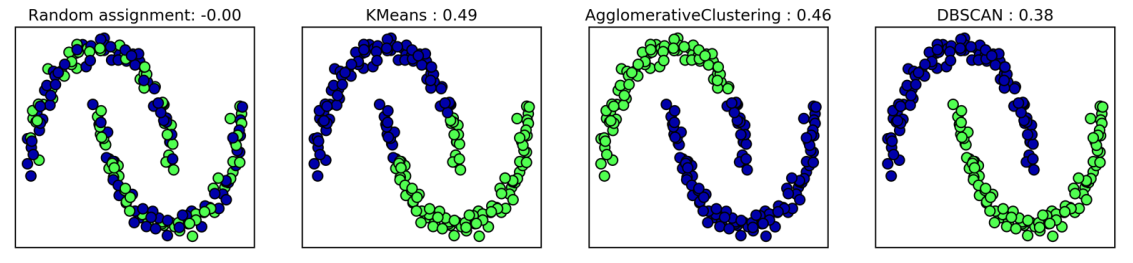
\includegraphics[scale=0.55]{../Imagen_Machine/ComparDBSCAN2}
	\caption{Comparación de asignación aleatoria, k-medias, Agglomerative y DBSCAN en el conjunto de datos de {\ttfamily two\_moons} usando la puntuación de \emph{silhouette} no supervisada. El resultado más intuitivo de DBSCAN tiene una puntuación de \emph{silhouette} más baja que las asignaciones encontradas por k-medias}
	\label{ComparDBSCAN2}
\end{figure}

Como se puede ver, k-medias  obtiene la puntuación más alta de silhouette, a pesar de que podríamos  preferir el resultado generado por DBSCAN. Una estrategia ligeramente mejor para evaluar los clústeres es usar métricas de clustering basadas en la robustez.  Estos ejecutan un algoritmo después de añadir algo de ruido a los datos, o usando diferentes parámetros de configuración, y comparar los resultados. La idea es que si muchos parámetros del algoritmo y muchas perturbaciones en la data  devuelven el mismo resultado, es probable que sea confiable.  Desafortunadamente, esta estrategia no está implementa en {\ttfamily scikit-learn} al momento de escribir este libro.\\

 Incluso si obtenemos una técnica de  clúster muy robusta, o una puntuación  muy alta de \emph{silhouette}, todavía no conocemos si hay algún significado semántico en el agrupamiento, o si el agrupamiento
refleja un aspecto de los datos que nos interese.  

Volvamos al ejemplo de imágenes de la cara.  Esperamos encontrar grupos de rostros similares, digamos, hombres y mujeres, ancianos y jóvenes, o personas con barba y sin barba.

Digamos que agrupamos el datos en dos clusters,  y todos los algoritmos están de acuerdo sobre qué puntos deben agruparse juntos.  Todavía no sabemos si los grupos que se encuentran corresponden a alguna forma en conceptos que nos interesan. Podría ser que encontraron vistas laterales versus vistas frontales o fotos tomadas de noche versus fotos tomadas durante el día, o fotos tomados con iPhones versus imágenes tomadas con teléfonos Android.  La única manera de saber si la agrupación corresponde a algo que nos interese es analizar  los clústers manualmente. 
 

\subsection{Comparación de los algoritmos sobre la dataset de caras}


Apliquemos los algoritmos de k-means, DBSCAN, y Agglomerative a la dataset Wild  de caras  etiquetadas, y veamos si alguno de ellos encuentra alguna estructura interesante. Utilizaremos la representación eigenface (caras propias) de los datos, tal como la genera {\ttfamily PCA(whiten=True)}, con 100 componentes:


\begin{lstlisting}  % [frame=single]	

In[71]: # extract eigenfaces from lfw data and transform data
        from sklearn.decomposition import PCA
        pca = PCA(n_components=100, whiten=True, random_state=0)
        pca.fit_transform(X_people)
        X_pca = pca.transform(X_people)


\end{lstlisting} 


Como vimos antes,  esta es una representación más semántica de las imágenes de la cara que los píxeles en bruto; y  también hará que el cálculo sea más rápido. Un buen ejercicio sería ejecutar los siguientes experimentos sobre la data  original, sin PCA, y ver si se encuentran grupos similares.


\subsubsection{Analizando la data de caras con DBSCAN}
 
 Comenzamos  aplicando  DBSCAN, que acabamos de discutir:

\begin{lstlisting} 

In[72]: # apply DBSCAN with default parameters
        dbscan = DBSCAN()
        labels = dbscan.fit_predict(X_pca)
        print("Unique labels: {}".format(np.unique(labels)))

Out[72]:
    
    Unique labels: [-1]

\end{lstlisting} 



Vemos que todas las etiquetas devueltas son -1, por lo que todos los datos fueron etiquetados como "{}ruido"{}  por DBSCAN. Hay dos cosas que podemos cambiar para mejorar este resultado: podemos hacer el {\ttfamily eps} más alto, para expandir la vecindad de cada punto, y configurar el {\ttfamily min\_samples} más bajo, para considerar grupos más pequeños (grupos con menos puntos) como clúster. Intentemos primero cambiando {\ttfamily min\_samples}:


\begin{lstlisting}  % [frame=single]	


In[73]: dbscan = DBSCAN(min_samples=3)
        labels = dbscan.fit_predict(X_pca)
        print("Unique labels: {}".format(np.unique(labels)))

Out[73]:
    
    Unique labels: [-1]

\end{lstlisting} 


Incluso cuando se consideran grupos de tres puntos, todo está etiquetado como ruido. Por 
lo tanto, tenemos que aumentar {\ttfamily eps}:

\begin{lstlisting}  % [frame=single]	

In[74]: dbscan = DBSCAN(min_samples=3, eps=15)
        labels = dbscan.fit_predict(X_pca)
        print("Unique labels: {}".format(np.unique(labels)))

Out[74]:

    Unique labels: [-1 0]


\end{lstlisting} 




Usando un {\ttfamily eps}  mucho más grande, como  15, obtenemos solo un clúster y puntos  ruido. Podemos usar este resultado para averiguar cómo se ve el "{}ruido"{ }   en comparación con el resto de los datos. Para entender mejor lo que está sucediendo, veamos cuántos puntos son ruido, y cuántos puntos están dentro del clúster:

\begin{lstlisting}  

In[75]: # Cuenta el numero de puntos en los grupos y del ruido.
        # El contador bincount no permite numeros negativos,
        # asi que tenemos que sumar 1.
        # El primer numero del resultado corresponde a los puntos ruido.
        print("Numero de puntos por grupo: {}".format(
               np.bincount(labels + 1)))

Out[75]:
   
   Numero de puntos por grupo: [ 27 2036]

\end{lstlisting} 


Hay muy pocos puntos  ruido, sólo 27, por lo que podemos verlos a todos 
(Figura \ref{CarasDBSCAN1}):

\begin{lstlisting} 

In[76]: noise = X_people[labels==-1]
   
        fig, axes = plt.subplots(3, 9, 
                                 subplot_kw={'xticks': (), 'yticks': ()},
                                 figsize=(12, 4))
        for image, ax in zip(noise, axes.ravel()):
            ax.imshow(image.reshape(image_shape), vmin=0, vmax=1)
     
\end{lstlisting} 



\begin{figure}[h!]
	\centering
	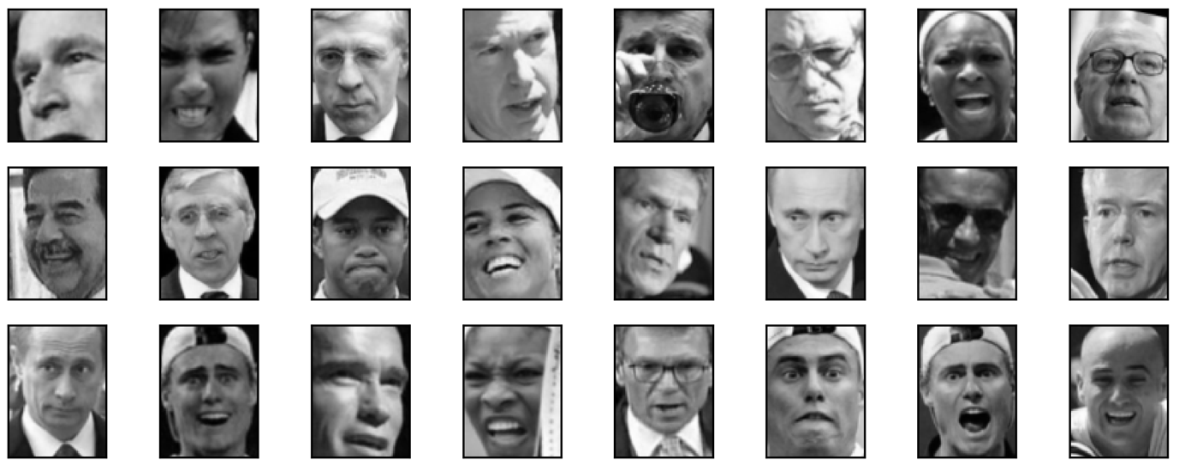
\includegraphics[scale=0.55]{../Imagen_Machine/CarasDBSCAN1}
	\caption{Muestras del conjunto de datos de las caras etiquetadas como ruido por DBSCAN}
	\label{CarasDBSCAN1}
\end{figure}


Comparando estas imágenes con la muestra aleatoria de las  imágenes de caras  de la figura \ref{Caras1}, podemos adivinar por qué fueron etiquetados como ruido: la quinta imagen en la primera fila muestra una persona  bebiendo en un vaso, hay imágenes de personas con sombreros, y en la última
imagen hay una mano delante de la cara de la persona. Las otras imágenes contienen extraños puntos de vista,  recortardas,  que son demasiado cercanos o demasiados anchos.\\

Este tipo de análisis, tratando de encontrar "{}lo extraño"{}, se llama detección de valores atípicos. Si
esta fuese una aplicación real, podríamos intentar hacer un mejor trabajo recortando imágenes, para obtener
datos más homogéneos. Es poco lo que podemos hacer con la gente en las fotos a veces usando sombreros, bebiendo o sosteniendo algo frente a sus caras, pero es bueno saber que éstos son asuntos en los datos que cualquier algoritmo que podamos aplicar necesita manejar.\\

Si queremos encontrar clusters más interesantes en lugar de uno sólo grande, necesitamos configurar el {\ttfamily eps}  más pequeño, algo entre  15 y 0.5 (0.5 es el  valor por defecto).  Veamos  que resulta con  valores diferentes {\ttfamily eps}:


\begin{lstlisting}  % [frame=single]	

In[77]: for eps in [1, 3, 5, 7, 9, 11, 13]:
            print("\neps={}".format(eps))
            dbscan = DBSCAN(eps=eps, min_samples=3)
            labels = dbscan.fit_predict(X_pca)
            print("Clusters present: {}".format(np.unique(labels)))
            print("Cluster sizes: {}".format(np.bincount(labels + 1)))

Out[78]:

    eps=1
    Clusters present: [-1]
    Cluster sizes: [2063]
    
    eps=3
    Clusters present: [-1]
    Cluster sizes: [2063]

    eps=5
    Clusters present: [-1]
    Cluster sizes: [2063]
    
    eps=7
    Clusters present: [-1 0 1 2 3 4 5 6 7 8 9 10 11 12]
    Cluster sizes: [2006 4 6 6 6 9 3 3 4 3 3 3 3 4]
    
    eps=9
    Clusters present: [-1 0 1 2]
    Cluster sizes: [1269 788 3 3]
    
    eps=11
    Clusters present: [-1 0]
    Cluster sizes: [ 430 1633]
    
    eps=13
    Clusters present: [-1 0]
    Cluster sizes: [ 112 1951]

\end{lstlisting} 


Para configuraciones bajas de {\ttfamily eps}, todos los puntos están etiquetados como ruido. 
Para {\ttfamily eps} = 7, obtenemos  2006  puntos ruido,  y 12  grupos más pequeños. Para {\ttfamily eps} = 9,  todavía  obtenemos muchos puntos ruido, pero obtenemos un grupo grande y algunos grupos más pequeños. A partir de {\ttfamily eps} = 11, obtenemos un  sólo grupo  grande y los puntos ruido.\\


Es interesante notar que sólo  hay  un grupo grande. A lo sumo, hay un grupo grande que contiene la mayoría de los puntos y algunos grupos más pequeños. Esto indica que no hay dos o tres tipos diferentes de imágenes de rostros en los datos que son muy distintos, sino que todas las imágenes son más o menos igualmente similares al (o diferente del) resto.\\


Los resultados para {\ttfamily eps} = 7 se ven más interesantes, con muchos grupos pequeños. Podemos investigar  esta agrupación con más detalle visualizando todos los puntos en cada uno de los 13
pequeños grupos (Figura \ref{VistaInverT}):

\begin{lstlisting}  

In[78]: dbscan = DBSCAN(min_samples=3, eps=7)
        labels = dbscan.fit_predict(X_pca)
        for cluster in range(max(labels) + 1):
            mask = labels == cluster
            n_images = np.sum(mask)
            fig, axes = plt.subplots(1, n_images, 
                                     figsize=(n_images * 1.5, 4),
                                     subplot_kw={'xticks':(), 'yticks': ()})
            for image, label, ax in zip(X_people[mask],
                                        y_people[mask], axes):
       
                ax.imshow(image.reshape(image_shape), vmin=0, vmax=1)
                ax.set_title(people.target_names[label].split()[-1])

\end{lstlisting} 


%  \newpage
%\addtolength{\voffset}{-3cm}
\begin{figure}[h!]
	\centering
	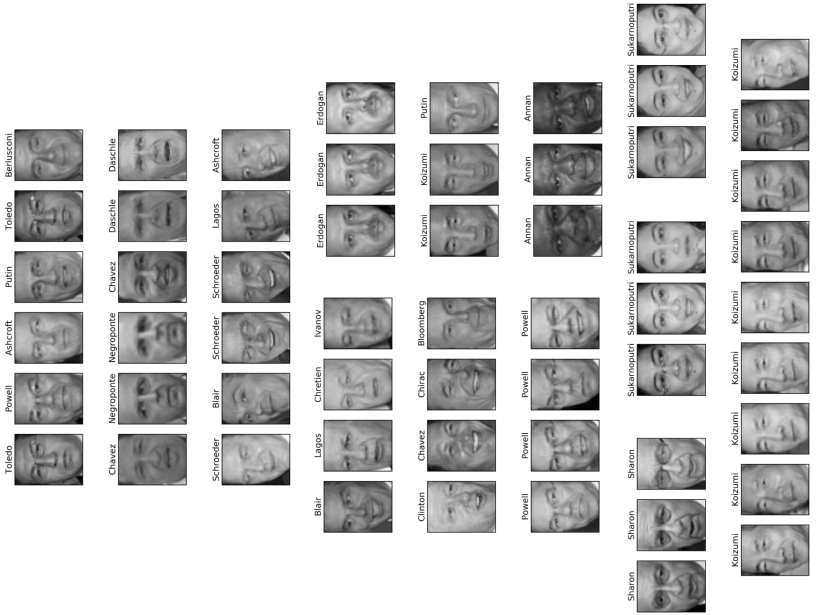
\includegraphics[width=16.6cm, height=13cm, angle=-90]{../Imagen_Machine/VistaInverT}
	\caption{Clusters encontrados por DBSCAN con eps = 7}
	\label{VistaInverT}
\end{figure}
%\addtolength{\voffset}{4cm}	


Algunos de los grupos corresponden a las personas con caras muy distintas (dentro de esta dataset), como Sharon o Koizumi. Dentro de cada grupo, la orientación de la cara es también bastante fijo, así como la expresión facial.  Algunos de los clusters contienen caras de multiples personas, pero comparten una orientación y expresión similares.\\

Esto concluye el análisis con el algoritmo DBSCAN aplicado sobre la dataset de  caras (faces). Como puede ver,  en este caso  hicimos un análisis manual, muy  distinto del enfoque de búsqueda  automático que podríamos utilizar con el aprendizaje supervisado basado en la puntuación $R^{2}$ o exactitud.\\

Ahora veamos las técnicas de k-medias y  agglomerative  aplicado a la dataset de caras.




\subsubsection{Analizando la dataset de caras con k-means}


 En la sección anterior, vimos que no fue posible crear más de un  clúster grande usando DBSCAN.  Con las técnicas de   clustering Agglomerative  y   k-means  hay mayor posiblilidad de  crear agrupos de tamaño uniforme, pero necesitamos configurar el número  de clústers. Podríamos establecer el número de clústeres igual al número  de personas conocidas en la dataset, pero es poco probable que un algoritmo de clusters no supervisado los recupere. En su lugar, podemos comenzar con un número bajo de clusters, como 10, lo que podría permitirnos analizar cada uno de los clusters:\\


\begin{lstlisting}  % [frame=single]	

In[79]: # extract clusters with k-means
        km = KMeans(n_clusters=10, random_state=0)
        labels_km = km.fit_predict(X_pca)
        print("Cluster sizes k-means: {}".format(np.bincount(labels_km)))

Out[79]:

    Cluster sizes k-means: [269 128 170 186 386 222 237 64 253 148]


\end{lstlisting} 



Como puedes ver, k-means divide los datos en grupos de tamaño relativamente similar entre 64 a 386. Este resultado es muy diferente al obtenido con  DBSCAN.\\

 Podemos analizar más a fondo el resultado de k-means visualizando los centros de clúster (Figure \ref{Kmedias10Clust}). Como en el caso del clúster en la representación generada por PCA, necesitamos rotar los centros de clúster de nuevo en el espacio original para visualizarlos, utilizando {\ttfamily pca.inverse\_transform}:\\

\begin{lstlisting}  % [frame=single]

In[80]: fig, axes = plt.subplots(2, 5, 
                                 subplot_kw={'xticks': (), 'yticks': ()},
                                 figsize=(12, 4))
        for center, ax in zip(km.cluster_centers_, axes.ravel()):
            ax.imshow(pca.inverse_transform(center).reshape(image_shape),
                      vmin=0, vmax=1)


\end{lstlisting} 


\begin{figure}[h!]
	\centering
	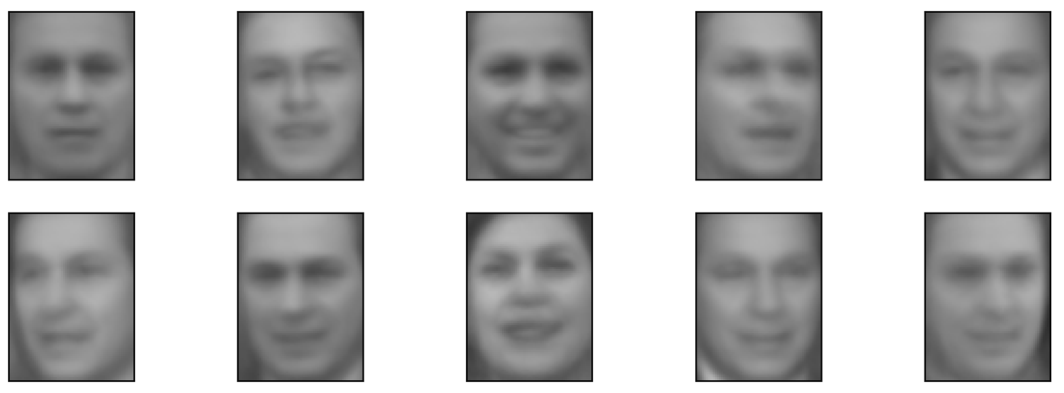
\includegraphics[scale=0.60]{../Imagen_Machine/Kmedias10Clust}
	\caption{Centros de clústeres encontrados por medios k al establecer el número de clústeres a 10}
	\label{Kmedias10Clust}
\end{figure}


Los centros de clusters encontrados por k-means son versiones muy suaves de caras. Esto no es
muy sorprendente, dado que cada centro tiene un promedio de 64 a 386 imágenes de caras. 
Trabajar con una representación PCA reducida aumenta la suavidad de las imágenes (en comparación
a las caras reconstruidas utilizando 100 dimensiones de PCA en la Figura \ref{Reconstruc}). 
El clustering  parece captar diferentes orientaciones de la cara, diferentes expresiones (el tercer centro de clúster parece mostrar una cara sonriente) y la presencia de cuellos de camisa (ver el
penúltimo centro de clúster).\\


Para una vista más detallada, en la Figure \ref{3-44} se muestra  para cada centro de clúster las cinco
imágenes típicas en el clúster (las imágenes asignadas al clúster más cercanas al
centro del grupo) y las cinco imágenes más atípicas en el grupo (las imágenes asignadas a
el clúster más alejado del centro del clúster):

\begin{lstlisting} 

In[81]: mglearn.plots.plot_kmeans_faces(km, pca, X_pca, X_people,
                                        y_people, people.target_names)

\end{lstlisting} 



\begin{figure}[h!]
	\centering
	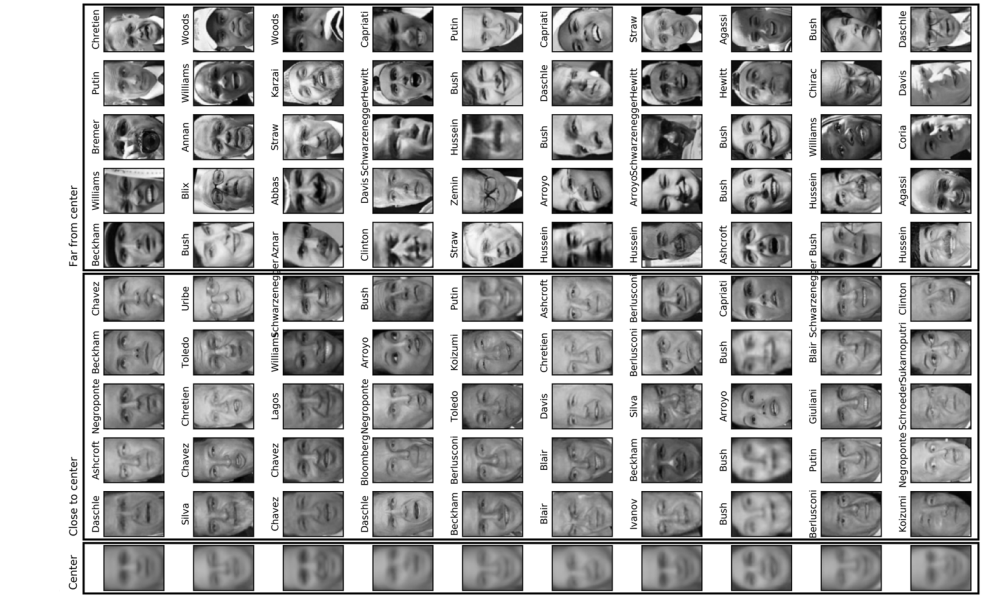
\includegraphics[width=16.1cm, height=13cm, angle=-90]{../Imagen_Machine/3-44}
	\caption{Imágenes de muestra para cada clúster encontrado por k-means, los centros de clúster están a la izquierda, seguidos por los cinco puntos más cercanos a cada centro y los cinco puntos asignados al clúster pero están más lejos del centro}
	\label{3-44}
\end{figure}



La figura \ref{3-44} confirma nuestra intuición sobre caras sonrientes para el tercer clúster, y también la importancia de la orientación para los otros clúster. Los puntos "{}atípicos"{}  no son muy similares a los centros de clúster, sin embargo, y su asignación parece algo arbitrario. Esto se puede atribuir al hecho de que las  particiones en k-medias, todos los puntos de datos y no tiene un concepto punto  "{}ruido"{ }, como en DBSCAN. Usando un mayor número de clústeres, el algoritmo podría encontrar distinciones más finas. Sin embargo, agregar más clústeres hace la inspección manual aún más difícil. 


\subsubsection{Analizando la data de caras con  Agglomerative}

 Ahora, veamos los resultados del  clúster Agglomerative:

\begin{lstlisting} 

In[82]: # extract clusters with ward agglomerative clustering
        agglomerative = AgglomerativeClustering(n_clusters=10)
        labels_agg = agglomerative.fit_predict(X_pca)
        print("Cluster sizes agglomerative: {}".format(
               np.bincount(labels_agg)))

Out[82]:

    Cluster sizes agglomerative: [255 623 86 102 122 199 265 26 230 155]


\end{lstlisting} 

El clúster agglomerative también produce grupos de tamaño relativamente igual, con tamaños de grupos entre 26 y 623. Estos son más desiguales que los producidos por k-medios, pero  incluso mucho más  que los producidos por DBSCAN. \\

Podemos calcular el ARI para medir si las  particiones de los datos generadas por agglomerative y k-medios son similares:

\begin{lstlisting}  % [frame=single]	

In[83]: print("ARI: {:.2f}".format(
               adjusted_rand_score(labels_agg, labels_km)))

Out[83]:

    ARI: 0.13

\end{lstlisting} 


Un ARI igual{}   0.13   {}significa que los grupos generados por las dos  técnicas de clústers  {\ttfamily "{}labels\_agg"{} }  y  {\ttfamily "{}labels\_km"{}} (sobre la data de caras), tienen  poco en  común. Esto no es muy sorprendente, dado del hecho de que los puntos más alejados de los centros de clúster parecen tener poco en común para  k-medias.\\

También es posible  gráficar el dendrograma (Figura \ref{DendoAglome}).   Limitaremos la profundidad del árbol en el gráfico, ya que la ramificación hacia los 2.063 puntos de datos individuales da como resultado una gráfico denso indescifrable:

%     irrazonablemente

\begin{lstlisting}  

In[84]: linkage_array = ward(X_pca)
        # now we plot the dendrogram for the linkage_array
        # containing the distances between clusters
        plt.figure(figsize=(20, 5))
        dendrogram(linkage_array, p=7, truncate_mode='level', no_labels=True)
        plt.xlabel("Sample index")
        plt.ylabel("Cluster distance")


\end{lstlisting} 



\begin{figure}[h!]
	\centering
	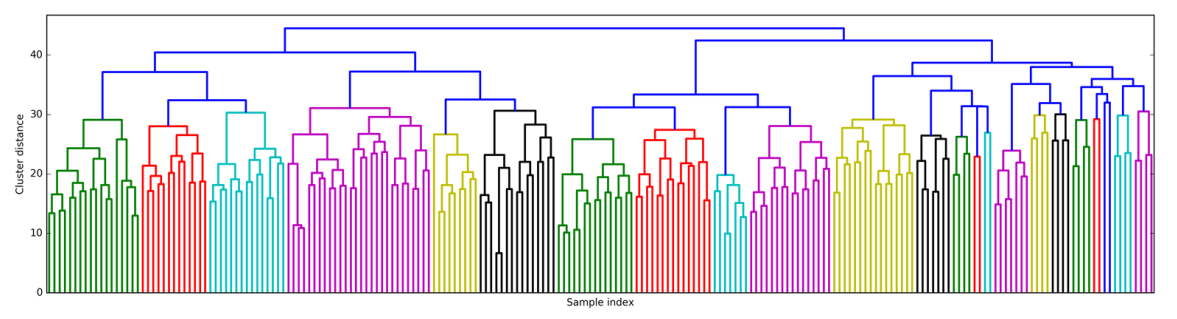
\includegraphics[scale=0.55]{../Imagen_Machine/DendoAglome}
	\caption{Dendrograma de agrupación aglomerante en el conjunto de datos de caras}
	\label{DendoAglome}
\end{figure}


Para crear 10 grupos, cortamos a través del árbol en la parte superior, donde hay 10 líneas verticales. En el dendrograma de la dataset  Toy, que se muestran en la Figura \ref{Dendog}, se puede ver por la longitud de las ramas que dos o tres grupos pueden capturar los datos apropiadamente. Para los datos de caras, no parece haber un punto de corte muy natural.   Hay algunas ramas que representan grupos más distintos, pero no parece haber un número particular de grupos que den un buen ajuste. Esto no es sorprendente, dados los resultados de DBSCAN, que intentó agrupar todos los puntos en un sólo grupo (casi todos juntos). \\



Visualicemos los 10 clusters, como lo hicimos anteriormente para k-means (Figura \ref{3-46}). Note que no hay noción de centro de clúster en la técnica de clúster Agglomerative (aunque podríamos calcular la media), y simplemente mostramos el primer par de puntos en cada clúster. Mostramos el número de puntos en cada clúster a la izquierda de la primera imagen:

\begin{lstlisting}  

In[85]: n_clusters = 10
        for cluster in range(n_clusters):
            mask = labels_agg == cluster
            fig, axes = plt.subplots(1, 10, 
                                     subplot_kw={'xticks': (), 'yticks': ()},
                                     figsize=(15, 8))
            axes[0].set_ylabel(np.sum(mask))
                 for image, label, asdf, ax in zip(X_people[mask],
                                                   y_people[mask],
                                                   labels_agg[mask], axes):
               ax.imshow(image.reshape(image_shape), vmin=0, vmax=1)
               ax.set_title(people.target_names[label].split()[-1],
                            fontdict={'fontsize': 9})


\end{lstlisting} 


\begin{figure}[h!]
	\centering
	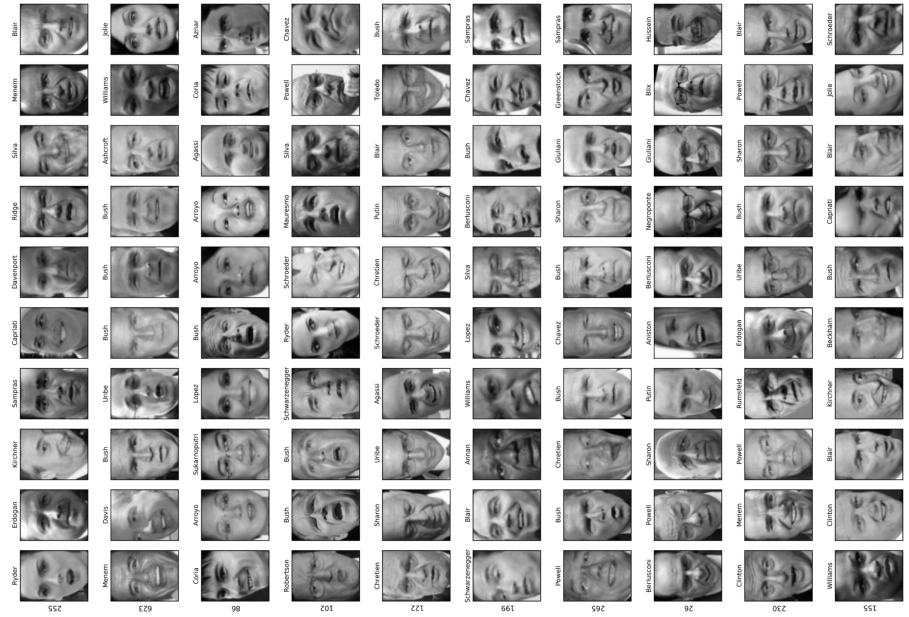
\includegraphics[width=16.4cm, height=13cm, angle=-90]{../Imagen_Machine/3-46}
	\caption{Imágenes aleatorias de los clústeres generados por el código en In[82], cada fila correspode a un clúster; el número a la izquierda indica el número de imágenes en cada clúster}
	\label{3-46}
\end{figure}


Mientras que algunos de los clústers parecen tener un tema semántico, muchos de ellos son demasiado grandes para ser realmente homogéneneos. Para obtener clústeres más homogéneneos, podemos correr el algoritmo de nuevo, esta vez con 40 clústeres, y seleccionar algunos de los clústeres que son particularmente interesantes (Figura \ref{Grupo}):


\begin{lstlisting}  % [frame=single]	

In[86]: # extract clusters with ward agglomerative clustering
        agglomerative = AgglomerativeClustering(n_clusters=40)
        labels_agg = agglomerative.fit_predict(X_pca)
        print("cluster sizes agglomerative: {}".format(
               np.bincount(labels_agg)))
   
        n_clusters = 40       # hand-picked "interesting" clusters
        for cluster in [10, 13, 19, 22, 36]: 
            mask = labels_agg == cluster
            fig, axes = plt.subplots(1, 15, 
                                     subplot_kw={'xticks': (), 'yticks': ()},
                                     figsize=(15, 8))                                
           cluster_size = np.sum(mask)
           axes[0].set_ylabel("#{}: {}".format(cluster, cluster_size))
           for image, label, asdf, ax in zip(X_people[mask], y_people[mask],
                                             labels_agg[mask], axes):
               ax.imshow(image.reshape(image_shape), vmin=0, vmax=1)
               ax.set_title(people.target_names[label].split()[-1],
                            fontdict={'fontsize': 9})
           for i in range(cluster_size, 15):
               axes[i].set_visible(False)

Out[86]:

    cluster sizes agglomerative:
    [ 58 80 79 40 222 50 55 78 172 28 26 34 14 11 60 66 152 27
      47 31 54 5 8 56 3 5 8 18 22 82 37 89 28 24 41 40
      21 10 113 69]


\end{lstlisting} 




\begin{figure}[!h!tbp]
	\begin{subfigure}[b]{\textwidth}
		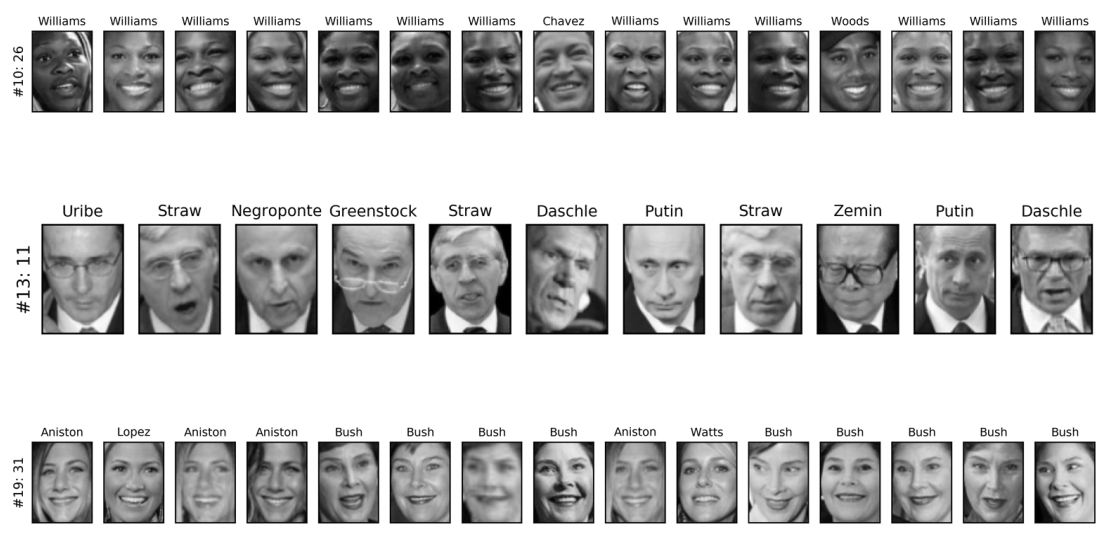
\includegraphics[scale=0.57]{../Imagen_Machine/G1}
		%	\caption{ }
		%	\label{  }
	\end{subfigure}
	\hfill
	\begin{subfigure}[b]{\textwidth}
		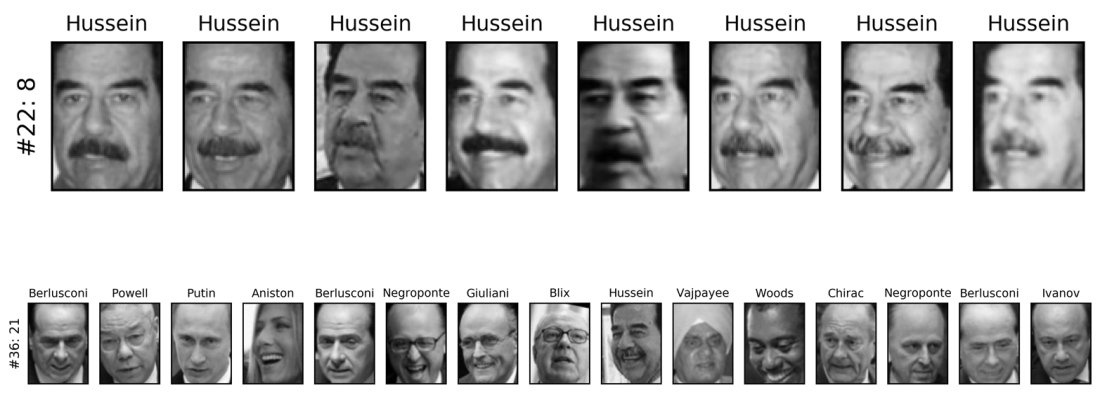
\includegraphics[scale=0.57]{../Imagen_Machine/G2}
		%	\caption{Segunda imagen.}
		%	\label{fig:f2}
	\end{subfigure}
	\caption{Imágenes de clústeres seleccionados encontrados por el clúster agglomerative al establecer el número de clústeres igual a 40. El texto a la izquierda muestra el índice del clúster y el número total de puntos en el clúster}
	\label{Grupo}
\end{figure}


\noindent Aquí, el clúster  parece haber seleccionado    "{ }piel oscura y sonriente"{},  "{ }camisa con cuello"{}, "mujer sonriendo"{}, "Hussein"{} y "frente alta.{}"{ }    También podríamos encontrar estos clústers altamente similares usando el dendrograma, si hiciéramos un análisis más detallado.


\newpage

\subsection{Resumen de los métodos de agrupación}

En esta sección se ha analizado y mostrado que  aplicar y evaluar los clústers es un procedimiento altamente cualitativo, y a menudo más útil en la fase exploratoria del análisis de datos. 

Analizamos tres algoritmos de agrupamiento: k-means, DBSCAN, y Agglomerative; los tres tienen una manera de controlar la densidad de la agrupación (número de elementos o densidad por grupo).  k-means y Agglomerative le permiten especificar el número de clústeres deseados, mientras que DBSCAN le permite definir la proximidad utilizando el parámetro {\ttfamily eps}, que influye indirectamente en el tamaño del clúster. Los tres métodos se pueden utilizar en  datas grandes  de la vida real, además son fácilmente comprensibles, y premite clúste en muchos grupos.\\

Cada uno de los algoritmos tiene  diferentes fortalezas.   k-means permite una cacterización de los clústeres usando las medias del clúster. También se puede ver como un método de descomposición, donde cada punto de datos está representado por su centro de clúster.  DBSCAN permite la detección de "{}puntos  ruido"{}  que no están asignados a ningún clúster, y puede ayudar a determinar automáticamente el número de clústeres. A diferencia de los otros dos métodos, DBSCAN permite formas declúster complejos, como vimos en el ejemplo de {\ttfamily two\_moons};  algunas veces produce grupos de tamaño muy diferente, que puede ser una fuerza o una debilidad. El clúster  Agglomerative  puede proporcionar toda una jerarquía de posibles particiones de los datos, que pueden ser fácilmente inspeccionados a través de dendrograma.





\section{Resumen y Perspectivas}

 Este capítulo introdujo una serie de algoritmos de aprendizaje  no supervisado que se pueden aplicar en el análisis de datos exploratorios y el preprocesamiento. Tener la representación correcta de los datos es a menudo crucial para que el aprendizaje supervisado o no supervisado tenga éxito, y los métodos de preprocesamiento y descomposición juegan un papel importante en la preparación de datos.



La descomposición, el aprendizaje múltiple y los clusters son herramientas esenciales para mejorar la comprensión de los datos, y  pueden ser las únicas formas de dar sentido a sus datos en
 ausencia de información  supervisada. 
 
 




\noindent Incluso en un entorno supervisado, las herramientas  exploratoratorias son de gran importancia  para una mejor comprensión de las propiedades de los datos. 
 Con frecuencia es difícil  cuantificar  la utilidad de un algoritmo no supervisado, aunque esto no debe  disuadirlo de usarlos para recopilar información de sus datos.

Con estos métodos debajo de su cinturón, ahora está equipado con todos los algoritmos esenciales   del aprendizaje automático que los profesionales  usan hoy en  día.\\

 


Le recomendamos que pruebe los métodos de agrupación y descomposición tanto en la data   bidimensional  Toy,  como en dataset del mundo real incluidos en scikit-learn, como la data de dígitos, iris y   cáncer.\\


				
				

\newpage

\vspace{-2cm}	
\hspace{-1cm}
{\fcolorbox{red}{white}{ 		
		\begin{minipage}[16cm]{13.5cm}    %   centrado, largo y ancho                {14cm} 
			\vspace{0.4cm}	
			
			
			{\footnotesize{	
					
					\begin{center}
						{\bf{Resumen de la interfaz del estimador} }
					\end{center}	
					
					
					
					Un repaso brevemente sobre la API que presentamos en los capítulos \ref{Cap2}   y  \ref{Cap3}.
					Todos los algoritmos en {\ttfamily scikit-learn}, ya sea preprocesamiento, algoritmos de aprendizaje supervisado o  no supervisado, son implementados como clases. En {\ttfamily scikit-learn}  estas clases son llamadas estimadores. Para aplicar un algoritmo, primero tienes que instanciar un objeto de la clase en particular:\\
					
					
					%\begin{lstlisting}  % [frame=single]	
					
					In[87]:	{\scriptsize{\color{blue}
							from { \color{cyan}  sklearn.linear\_model} import {\color{cyan}   LinearRegression }
							
					\hspace{1.1cm}logreg = LogisticRegression()   } }  \\            
					
					
					
					% \end{lstlisting}
					
					
					La clase  estimador contiene el algoritmo y también almacena el modelo aprendido
					de la data usando el algoritmo. \\
					
					
					Se debe configurar cualquier parámetro del modelo  objeto a construir.
					Estos parámetros incluyen regularización, control de complejidad, número de clusters para
					encontrar, etc.  Todos los estimadores tienen un método de ajuste, que se utiliza para
					construir el modelo.  El método {\ttfamily fit} siempre requiere como primer argumento la data X, representados como una matriz {\ttfamily NumPy} o una matriz  sparse  de {\ttfamily SciPy}, donde cada fila representa un único punto de la data. Los datos X  siempre se supone que es una matriz {\ttfamily NumPy} o una matriz sparse  {\ttfamily SciPy} que contiene entradas continuas (floating-point).  Los algoritmos supervisados  también requieren un argumento $y$, que es una matriz {\ttfamily NumPy} unidimensional que contiene valores objetivos para regresión o clasificación (es decir, las etiquetas o respuestas de salida conocidas).\\
					
					
					
					Hay dos maneras principales de aplicar un modelo aprendido en   {\ttfamily scikit-learn}. Para crear una predicción  en forma de una nueva salida como $y$, se utiliza el método de  {\ttfamily predict}. Para crear una nueva representación de los datos de entrada X, se utiliza el método {\ttfamily transform}. La Tabla \ref{Tabla1} presenta un resumen de la implementación de los métodos {\ttfamily predict}  y  {\ttfamily transform}.\\
					
					
					
					
					
					%\begin{table}[htbp]
					%	\caption{Resumen de la API {\ttfamily scikit-learn}}
					
					Tabla \ref{Tabla1}.  Resumen de la API {\ttfamily scikit-learn}
					
					\begin{tabular}{l l }
						%\caption{Resumen de la API {\ttfamily scikit-learn}}
						\multicolumn{2}{|>{\columncolor{vino}}c|}{\color{white}\bf estimator.fit(x\_train, [y\_train])}\\
						\multicolumn{2}{|>{\columncolor{vino}}c|}{\color{white}\bf estimator.predict(X\_text) \hspace{0.15cm}  estimator.transform(X\_test)}\\
						\hline
						Classification &\hspace{3cm} Preprocessing\\	
						Regression     &\hspace{3cm} Dimensionality reduction\\
						Clustering     &\hspace{3cm} Feature extraction\\
						&\hspace{3cm} Feature selection \\
						\arrayrulecolor{vino}\hline
					\end{tabular}\label{Tabla1} \\
					%\end{table}
					\vspace{0.2cm}
					
					Además, todos los modelos supervisados tienen un método  que permite una evaluación del modelo, es   {\ttfamily score(X\_test, y\_test)}. En  la Tabla \ref{Tabla1},{ } {\ttfamily  X\_train,   y\_train }   se refieren a los datos y etiquetas para entrenar, mientras que  {\ttfamily X\_test,   y\_test}  se refieren a los datos y etiquetas para  prueba (si es aplicable).\\
					
					
					
					% {\scriptsize{\color{blue} 
					%		from { \color{cyan}  sklearn.linear\_model} import {\color{cyan}   
					%		LinearRegression }           		logreg = LogisticRegression()   } }  \\ 
					
					
			} }
			
\end{minipage}  }}


											
   



\chapter{Ingeniería de Características y Representación de la Data}{\label{Cap4}}



\section{Introducción}



Hasta ahora, hemos asumido que los datos vienen como un    arreglo o una  matriz  bidimensional de números de puntos flotante (floatingpoint), donde cada columna es una característica continua que describe la data de puntos. Para muchas aplicaciones, esto no así  cómo se recopilan los datos.  Un tipo  de característica   particular  muy común son las características categóricas, también conocido como las características discretas, y  por lo general,  son no  numéricos.  La distinción entre las características categóricas y las características continuas es análoga para la distinción entre la clasificación y la regresión, sólo el  aporte de la  entrada más que  la salida. Los ejemplos de características continuas que hemos visto son  brillos de pixeles y las medidas del tamaño en flores Iris, y   ejemplos de características categóricas son la marca de un producto, el color de un producto o  el departamento de ventas (como libros, ropa, hardware, etc.).  Éstas son propiedades que puede describir un producto, pero no varían en forma continua. Un producto que pertenece  al departamento de ropa o al departamento de libros. No hay opción en el medio libros y ropas, y ningún orden natural para las diferentes categorías (los libros no son mayores o menos que la ropa, el hardware no está entre libros y ropas).\\

 Es muy importante considerar la natuarleza de los datos; ya que estos  tendrán un enorme efecto sobre el desempeño del modelo de aprendizaje  automático. En los Capítulos \ref{Cap2}  y \ref{Cap3} vimos que re-escalar de los datos es muy importante; puede suceder que si no se re-escalan los  datos (digamos, con  varianza  unitaria),   puede aparecer alguna diferencia  si representa una medida en centímetros o pulgadas.
 También vimos en el Capítulos \ref{Cap2}  que puede ser útil aumentar la data con características adicionales, como sumar interacciones (los productos) de características o polinomios más general.\\


La técnica que estudia  cómo representar mejor los datos para una aplicación particular es conocida  como Ingeniería de Característica\index{Ingeniería de Característica}, y es una de las principales tareas de científicos de datos y los profesionales  del aprendizaje automático tratando de resolver problemas del mundo real. La representación de los  datos en la forma correcta puede tener una mayor influencia sobre el rendimiento del modelo supervisado más que los parámetros exactos que se puedan seleccionar.\\


En este capítulo, primero abordaremos  el caso importante y muy común de características categóricas, y daremos algunos ejemplos de transformaciones útiles para combinaciones específicas de características y modelos.\\



\section{Variables Categóricas}

Como  ejemplo, usaremos la dataset de Ingresos de Adultos de los Estados Unidos, derivada de la base de datos  censos 1994. La tarea con la  data Ingresos es predecir si un trabajador tiene un ingreso superior o inferior a \$50,000. Las características en esta dataset incluyen la edad del trabajador, tipo de empleo (trabajador por  cuenta propia,  industria privada o empleado del gobierno, etcétera.), educación,  género,  horas de trabajo por la semana, ocupación, y otros. La tabla \ref{Tabla01}  muestra las primeras entradas de la  dataset Ingresos de Adultos.\\



El objetivo en este caso  es expresado como una tarea de clasificación con dos clases para el ingreso,   $<= 50k $  y  $ > 50k$. También se podría  predecir el ingreso exacto, y hacer esta tarea como una regresión.  Sin embargo, eso sería  más difícil, pero por ahora  nuestro interés es  la división del ingreso  para entender.\\

\hspace{-0.6cm} Tabla \ref{Tabla01}. La primeras  entradas de la data  Adultos
\vspace{-0.4cm} 
\begin{figure}[h!]
	%\centering
	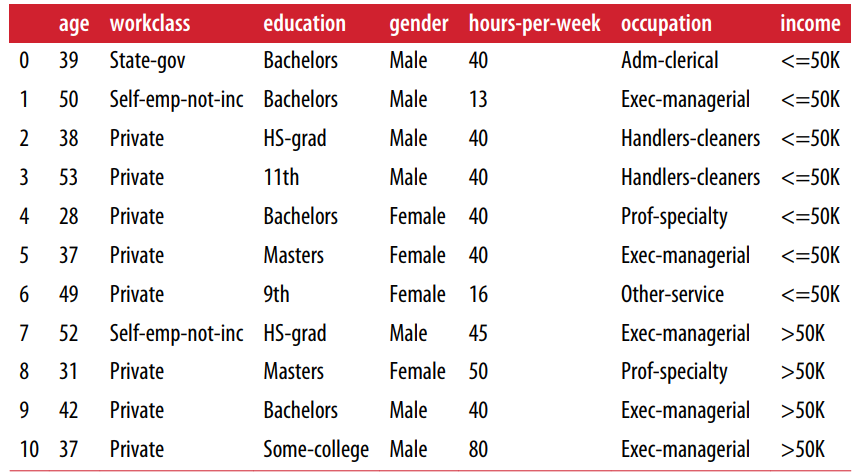
\includegraphics[scale=0.55]{Imagen_Machine/Tabla01}
\end{figure}\label{Tabla01} 

	
En esta data, la edad y las horas por la semana son características continuas, el cuál sabemos como se trata; el tipo de trabajo, educación,  sexo, y la ocupación son características  categóricas, sin embargo, todos ellos vienen de una lista fija de valores posibles, en una distinción de rango que denota una  propiedad cualitativa, en lugar de una cantidad.\\	
	



Como un punto de partida, digamos que queremos que un clasificador de regresión logística  aprenda  en esta data.  Sabemos  del Capítulo \ref{Cap2} que  una regresión logística hace predicciones   $\hat{y}$, mediante la siguiente fórmula:

\[ \hat{y} = w[0] * x[0] + w[1] * x[1] + ... + w[p] * x[p] + b > 0 \]


Donde $w[i]$ y  $b$ son coeficientes aprendidos en el conjunto de entrenamiento,   and $x[i]$ son las entradas de las características.    Esta fórmula tiene sentido cuando $ x[i]$ son números, pero cuando la $X[i]$ no son números no tiene sentido, como en el caso de $x[2]$  es "Masters"{} o "Bachelors".
Claramente necesitamos representar estos datos en alguna otra forma que permita aplicar el modelo regresión logística. 

En la  siguiente sección se explica cómo podemos  tratar este problema.
	
%  https://machinelearningmastery.com/one-hot-encoding-for-categorical-data/

\subsection{Codificación One-Hot  (one-hot-encoding) }	

%  Codificación única (One-Hot-Encoding) o  variables ficticias (Dummy Variables)
 
La forma más común para representar variables categóricas es usando la Codificación One-Hot   o  one-out-of-N\index{one-out-of-N}, también conocido como  variables dummy o variables ficticias. La idea detrás de las  variables dummy es reemplazar una variable categórica con una o más características nuevas que pueden tomar los  valores 0 y 1. Los valores 0 y 1 dan sentido a la fórmula de clasificación binaria lineal (y para todos  modelos en {\ttfamily{scikit-learn}}), y podemos representar  {\bf \emph{cualquier número de  categorías} }   introduciendo una nueva característica  por  categoría, como se describe aquí.\\


Digamos para la característica  workclass  (tipo de empleo)  los valores posibles  "{}Government Employee"{}  (empleado del gobierno) , "{}Private Employee"{}  (empleado privado) , "{}Self Employed"{} (empleado por cuenta propia) , y "{}Self Employed Incorporated"{}   (empleado por cuenta propia calificado).   Para codificar estos cuatro valores posibles, creamos cuatro características nuevas, designadas "{}Government Employee"{}, "{}Private Employee"{}, "{}Self Employed"{}, y "{}Self Employed Incorporated"{}.     
El valor de la nueva característica será  1 si el  tipo de empleo para esta  persona tiene el valor  correspondiente  y  0 en otro caso, así exactamente sólo una de las cuatro características nuevas será igual  1 para cada dato (en este caso la fila).  Por este motivo esta codificación es llamada  one-hot o one-out-of-N\index{codifecaión one-hot}.\\




El principio se ilustra en la Tabla \ref{Tabla02}, donde sólo la característica workclass  es codificada usando  cuatro nuevas características.  Al usar esta data en un algoritmo  machine learning,  descartaríamos la característica original workclass y sólo mantendríamos las nuevas  características con  0–1.  En la tabla  \ref{Tabla02} se codifica la característica workclass usando una codificación one-hot.\\	


\hspace{-0.6cm} Tabla \ref{Tabla02}. Característica workclass codificada con  one-hot
\vspace{-0.4cm} 
\begin{figure}[h!]
	%\centering
	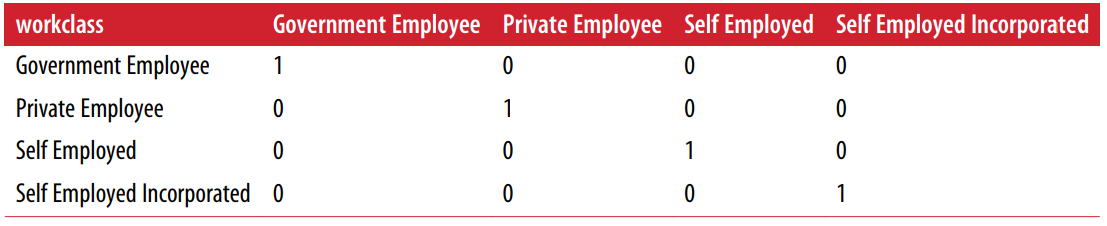
\includegraphics[scale=0.55]{Imagen_Machine/Tabla02}
\end{figure}\label{Tabla02} 

\newpage

\begin{minipage}[t]{0.2\textwidth}
	\centering\raisebox{\dimexpr \topskip-\height}{%
		
\includegraphics[width=\textwidth]{Imagen_Machine/Pajaro.png}}
\end{minipage}%\hfill
\begin{minipage}[t]{0.75\textwidth} 
	{\scriptsize	
	La codificación one-hot que usamos es muy similar, \:  pero no idéntica, a la codificación 
	dummy usada en Estadística. \: Por simplicidad, \: codificamos cada categoría con una característica binaria diferente. En  Estadística, es común  codificar una característica categórica con $k$ valores posibles diferentes en $k$–$1$  características (el último es representado como todos los ceros). Esto se hace  	para simplificar el análisis (técnicamente hablando,  esto evitará hacer que la matriz de datos sea deficiente en rango).}
\end{minipage} \\


Hay dos formas para convertir los datos  con la codificación one-hot a  variables  categóricas, mediante el uso de {\ttfamily pandas}  o  {\ttfamily scikit-learn}.  Al momento de escribir estas notas, el uso de  {\ttfamily pandas}  es un poco más fácil, así que elegimos  esta ruta. Primero cargamos la data usando {\ttfamily pandas} como un archivo de valores separados por comas  (CSV):

\begin{lstlisting}  	

In[2]:

   import pandas as pd
   # The file has no headers naming the columns, so we pass header=None
   # and provide the column names explicitly in "names"
   data = pd.read_csv("https://archive.ics.uci.edu/ml/
                       machine-learning-databases/adult/adult.data", 
                       header=None, index_col=False, 
                       names=['age', 'workclass', 'fnlwgt','education',
                              'education-num','marital-status', 'occupation',
                              'relationship', 'race', 'gender', 'capital-gain', 
                              'capital-loss', 'hours-per-week', 'native-country',
                              'income'])
   # For illustration purposes, we only select some of the columns
   data = data[['age', 'workclass', 'education', 'gender', 'hours-per-week',
                'occupation', 'income']]
   # IPython.display allows nice output formatting within the Jupyter notebook
   display(data.head())
   
\end{lstlisting}   


\hspace{-0.6cm} Tabla \ref{Tabla03}. Las primeras cinco filas de la data Adultos
\vspace{-0.4cm} 
\begin{figure}[h!]
	%\centering
	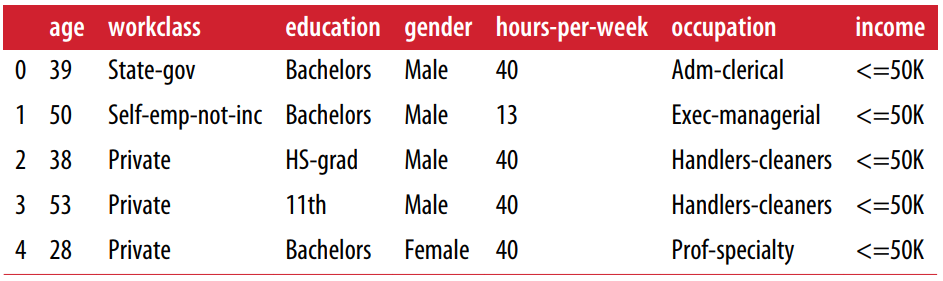
\includegraphics[scale=0.55]{Imagen_Machine/Tabla03}
\end{figure}\label{Tabla03} 
\newpage

\subsection{Verificación  de datos categóricos codificados en  cadena de caracteres (string)}
%  Checking string-encoded categorical data


Después de leer un conjunto de datos como este,  es buena práctica  comprobar primero si una columna contiene datos categóricos significativos. Cuando se trabaja con datos que fueron introducidos por seres humanos (por ejemplo, usuarios en un sitio web), podría no haber un conjunto fijo de categorías, y differencias en la ortografía y la capitalización podrían requerir preprocesamiento. Por ejemplo, podría ser que algunas personas especificaran el género como  "{}masculino"{} y  otras como "hombre"{},  y 
podríamos  querer representar estas dos entradas usando la misma categoría.   Una buena manera de comprobar el contenido de una columna es usando la función {\ttfamily value\_counts }  de una serie de pandas (el tipo de una sola columna en un DataFrame), para mostrarnos cuáles son los valores únicos y con qué frecuencia aparecen:

\begin{lstlisting}  

In[3]: print(data.gender.value_counts())

Out[3]:

   Male 21790
   Female 10771
   Name: gender, dtype: int64
  
\end{lstlisting} 

Podemos ver que hay exactamente dos valores para el género en este conjunto de datos, masculino y femenino, lo que significa que los datos ya están en un buen formato para ser representados utilizando la codificación One-Hot.  En una aplicación real, debe observar todas las columnas y verificar sus valores. En este caso lo vamos a omitir  por la brevedad.

 Hay una manera muy sencilla de codificar los datos en  {\ttfamily pandas}, usando la función {\ttfamily get\_dummies}, esta función  transforma automáticamente todas las columnas que tienen un tipo de objeto (como cadenas) o  categóricas (un concepto especial de {\ttfamily pandas} del que aún no hemos hablado):\\


\begin{lstlisting}%[frame=single]

In[4]:

   print("Original features:\n", list(data.columns), "\n")
   data_dummies = pd.get_dummies(data)
   print("Features after get_dummies:\n", list(data_dummies.columns))

Out[4]:

    Original features:
    ['age', 'workclass', 'education', 'gender', 'hours-per-week',
     'occupation', 'income']

   Features after get_dummies:
    ['age', 'hours-per-week', 'workclass_ ?', 'workclass_ Federal-gov',
     'workclass_ Local-gov', 'workclass_ Never-worked', 'workclass_ Private',
     'workclass_ Self-emp-inc', 'workclass_ Self-emp-not-inc',
     'workclass_ State-gov', 'workclass_ Without-pay', 'education_ 10th',
     'education_ 11th', 'education_ 12th', 'education_ 1st-4th',
      ...
     'education_ Preschool', 'education_ Prof-school', 
     'education_ Some-college','gender_ Female', 'gender_ Male', 
     'occupation_ ?', 'occupation_ Adm-clerical', 
     'occupation_ Armed-Forces', 'occupation_ Craft-repair',
     'occupation_ Exec-managerial', 'occupation_ Farming-fishing',
     'occupation_ Handlers-cleaners',
      ...
     'occupation_ Tech-support', 'occupation_ Transport-moving',
      'income_ <=50K', 'income_ >50K']

\end{lstlisting}


Puede ver que las características continuas edad y horas por semana no presentan cambios, mientras que las características categóricas se ampliaron en una nueva característica para cada valor posible 
(por categoría):

\begin{lstlisting}

In[5]:

   data_dummies.head()

Out[5]:

\end{lstlisting}

\hspace{-0.6cm} Tabla \ref{Tabla04}. Las primeras cinco filas de la data Ingresos
\vspace{-0.4cm} 
\begin{figure}[h!]
	%\centering
	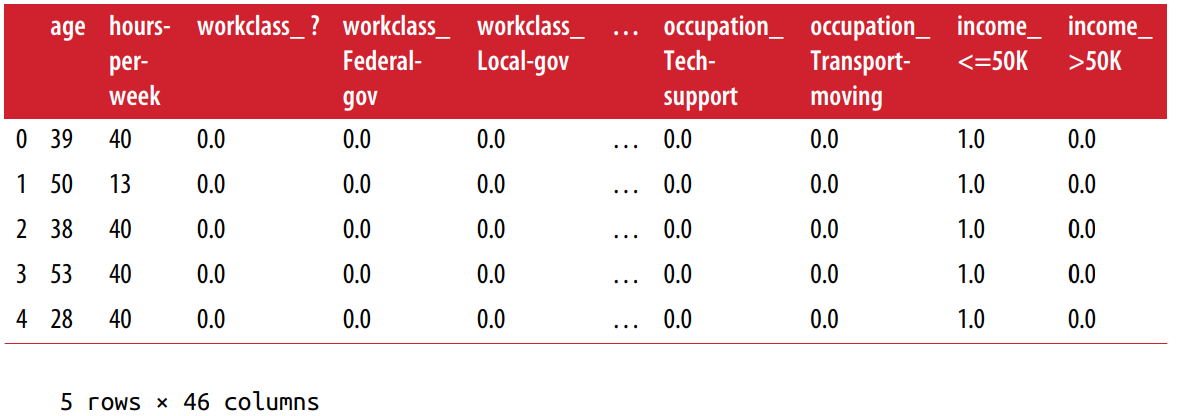
\includegraphics[scale=0.55]{Imagen_Machine/Tabla04}
\end{figure}\label{Tabla04} 

Ahora podemos usar el atributo {\ttfamily values}  para convertir la  {\ttfamily  DataFrame  data\_dummies  } en un arreglo  {\ttfamily  NumPy}  (matriz), y luego entrenar un modelo de aprendizaje automático sobre esa data. Debe tener cuidado al separar la variable  objetivo de los datos antes de entrenar un modelo (pues ahora está codificada en dos columnas de ingresos).    Incluyendo la variable  salida, o alguna propiedad derivada de la variable  salida, en la representación de características es un error muy común en la construcción de modelos de aprendizaje automático supervisado.


\begin{minipage}[t]{0.2\textwidth}
	\centering\raisebox{\dimexpr \topskip-\height}{%
		
\includegraphics[width=\textwidth]{Imagen_Machine/Escorpion}}
\end{minipage}%\hfill
\begin{minipage}[t]{0.75\textwidth} 
	{\scriptsize		
		Tenga cuidado: la indexación de columnas en pandas incluye el final del rango, así que  "{}age"{}:  "{}occupation\_ Transport-moving"{}   incluya  a   "{}occupation\_  Transport-moving"{}. Esto es diferente de dividir  un {\ttfamily array NumPy}, donde el final de un rango no se incluye: por ejemplo,  {\ttfamily  np.arange(11)[0:10] }  no incluye la entrada con el índice 10.\\}
\end{minipage}
\\

En este caso, extraemos sólo las columnas que contienen características, es decir, todas las columnas de  {\ttfamily age } a   {\ttfamily occupation\_  Transport-moving}. Este rango contiene todas las características pero no el objetivo:

\begin{lstlisting}
In[6]:

   features = data_dummies.ix[:, 'age':'occupation_ Transport-moving']
   # Extract NumPy arrays
   X = features.values
   y = data_dummies['income_ >50K'].values
   print("X.shape: {} y.shape: {}".format(X.shape, y.shape))

Out[6]:

    X.shape: (32561, 44) y.shape: (32561,)
    
\end{lstlisting}

Ahora los datos se representan de una manera que el {\ttfamily scikit-learn} puede trabajar,  y podemos proceder como de costumbre:

\begin{lstlisting}
In[7]:

   from sklearn.linear_model import LogisticRegression
   from sklearn.model_selection import train_test_split
   X_train, X_test, y_train, y_test = train_test_split(X, y, random_state=0)
   logreg = LogisticRegression()
   logreg.fit(X_train, y_train)
   print("Test score: {:.2f}".format(logreg.score(X_test, y_test)))

Out[7]:
   
   Test score: 0.81
\end{lstlisting}



\newpage



\begin{minipage}[t]{0.2\textwidth}
	\centering\raisebox{\dimexpr \topskip-\height}{%
		
\includegraphics[width=\textwidth]{Imagen_Machine/Escorpion}}
	%	\captionof{figure}{Caption for fig 1}
	%	\label{fig1}
	%	\includegraphics[width=\textwidth]{example-image-b}
	%	\captionof{figure}{Caption for fig 2}
	%	\label{fig2}
\end{minipage}\hfill
\begin{minipage}[t]{0.75\textwidth} 
	{\scriptsize
		En este ejemplo, ejecutamos  a {\ttfamily get\_dummies} sobre la DataFrame que contiene
		tanto la data de  entrenamiento como la de prueba. Esto es importante para asegurar que
		los valores de las categorías se representan de la misma forma tanto en el conjunto de
		entrenamiento y como en el de prueba.\\		
		Imagine que tenemos la data  entrenamiento y prueba en dos dataframes diferentes.  Si el valor 
		"{}Private Employee"{}   para la característica  workclass no aparece en la data de prueba, {\ttfamily pandas} asumirán que sólo hay tres valores posibles para esta característica y creará solo tres nuevas características ficticias (dummy).  				
		Ahora la data de entrenamiento y prueba tienen diferentes número de características, y no podemos aplicar el modelo que aprendido en la data de entrenamiento al  prueba. Peor aún, imagina la característica  workclass  tiene los valores  "{}Government Employee"{} y "{}Private Employee"{}  en el conjunto de entranamiento, y  "Self Employed"{}  y  "{}Self Employed Incorporated"{}   en el conjunto de prueba.
		En ambos casos, {\ttfamily pandas} crearán dos nuevas características ficticias, por lo que los datos codificados en la dataframe  tendrán el  mismo número de caracteísticas. Sin embargo, las  características ficticias tienen significados completamente diferentes en la data de entrenamiento y en la de  prueba. La columna que significa  "{}Government Employee"{}  para el conjunto de entrenamiento codificaría  "{}Self Employed"{}  para el conjunto de prueba.	\\ 
	 Si construimos un modelo de aprendizaje automático sobre estos datos, funcionaría muy mal, 
	 porque supondría que las columnas significan la misma cosa   (porque están en la misma posición) cuando en realidad tienen significados muy diferentes.  Para solucionar esto, se ejecuta a {\ttfamily get\_dummies} en una DataFrame que contiene los  puntos de datos de entrenamiento y prueba, o asegúrese de que los nombres de las columnas sean los mismos para la data de entrenamiento y prueba, después de  ejecutar  {\ttfamily get\_dummies}, para segurarse de que tengan el misma semántica.}\\
	\end{minipage}




\subsection{Números que se pueden codificar como categorías}
% Numbers Can Encode Categoricals


En el ejemplo de la data  Adultos, las variables categóricas se codificaron como cadenas.
Por un lado, eso abre la posibilidad de errores ortográficos, y además, marca claramente una variable  categórica.   Genearlmente las variables categóricas son codificadas como enteros,  ya sea por facilidad de almacenamiento o debido a la forma en que se recopilan los datos.  Por ejemplo, imagine que los datos del censo en la data  Adultos se recopilaron mediante una pregunta y las respuestas para la clase de trabajo se registraron como 0 (primer casilla etiquetada), 1 (segunda  casilla etiquetada), 2 (casilla marcada tercera), y así sucesivamente. 
Ahora la columna contendrá números del 0 al 8, en lugar de cadenas como  "{}Private"{}, y no será inmediatamente  obvio para alguien que vea la tabla  representada el en conjunto de datos, identificar si se  trata una  variable como continua o categórica.   Sin embargo,   conociendo  que los números indican el estado laboral,  queda claro que estos son estados muy distintos y  no deben ser modelado por una  variable continua. \\




\begin{minipage}[t]{0.2\textwidth}
	\centering\raisebox{\dimexpr \topskip-\height}{%
		
\includegraphics[width=\textwidth]{Imagen_Machine/Escorpion}}
	%	\captionof{figure}{Caption for fig 1}
	%	\label{fig1}
	%	\includegraphics[width=\textwidth]{example-image-b}
	%	\captionof{figure}{Caption for fig 2}
	%	\label{fig2}
\end{minipage}\hfill
\begin{minipage}[t]{0.75\textwidth} 
	{\scriptsize	
	Las características categóricas generalmente se codifican con números enteros. 	El hecho que  sean números no significa que deban ser tratados necesariamente como características continuas.  No siempre está claro si una característica de número entero debe ser tratada como continua o discreta.
	Si no hay un  orden entre la semántica que se codifica (como en el ejemplo de clase de trabajo), la característica debe ser tratado como discreta. 	 Para otros casos, la mejor codificación depende de la tarea particular,   la  data y de qué tipo de algoritmo de aprendizaje automático se utiliza.\\}
\end{minipage}\\


La función {\ttfamily get\_dummies} en {\ttfamily pandas} trata todos los números como continuos 
y no creará variables dummy para ellos. Para evitar esto, puede hacer uso de  {\ttfamily OneHotEncoder} 
de  {\ttfamily  scikit-learn}, para el cual puede especificar cuales  variables son continuas y 
cuáles son discretas, o convertir columnas numéricas en Dataframe de cadenas (strings). Para ilustrar este proceso vamos a crear un objeto tipo DataFrame con dos columnas, una con  cadenas y la  otra con h enteros:

\begin{lstlisting}
In[8]:

   # create a DataFrame with an integer feature and a categorical string 
   # feature
   demo_df = pd.DataFrame({'Integer Feature': [0, 1, 2, 1],
                           'Categorical Feature': ['socks', 'fox', 
                                                   'socks', 'box']})
   display(demo_df)

\end{lstlisting}


\noindent El resultado se muestra en la tabla \ref{Tabla05}.
%\vspace{-0.2cm}
\begin{table}[!h]
	\hspace{0.1cm} \vspace{-0.1cm}	\caption{DataFrame que contiene dos características  categórica, una  string    y la otra con enteros}	
	\label{Tabla05}	
	\hspace{-0.4cm} \begin{tabular}{  l  }
		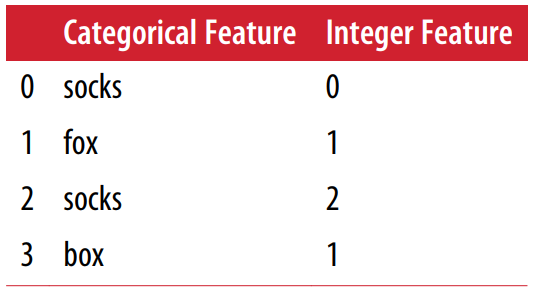
\includegraphics[scale=0.45]{Imagen_Machine/Tabla05}
	\end{tabular}
\end{table}




Usando {\ttfamily get\_dummies} sólo codificará la característica  string y no cambiará la característica de enteros, como puedes ver en la Tabla \ref{Tabla61}.


\begin{lstlisting}%[frame=single]

In[9]:
   
   pd.get_dummies(demo_df)


\end{lstlisting}
%\vspace{-0.5cm}
\begin{table}[!h]
	\hspace{0.1cm} \vspace{-0.1cm}	\caption{Una versión de codificación One-hot  de los datos de la Tabla \ref{Tabla05}, dejando la característica de entero  sin cambiar}	
	\label{Tabla61}	
\hspace{-0.4cm}	\begin{tabular}{  l  }
		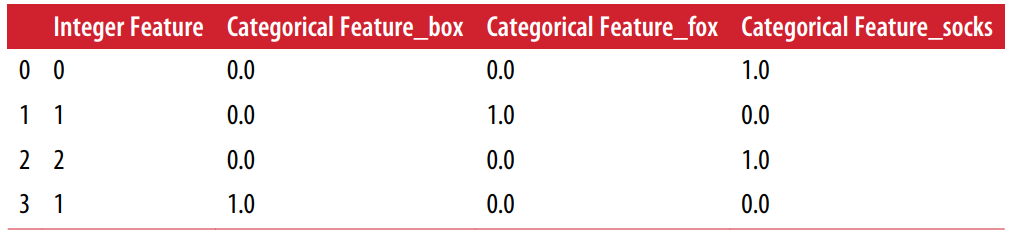
\includegraphics[scale=0.55]{Imagen_Machine/Tabla61}
	\end{tabular}
\end{table}

Si desea que se creen variables   dummy (ficticias) para la columna "{}característica entera"{}, puede enumerar explícitamente las columnas que desea codificar utilizando el parámetro columnas. A continuación, ambas características se considerarán categóricas (véase en la Tabla \ref{Tabla71}): 
	
	\begin{lstlisting}%[frame=single]
	
In[10]:

   demo_df['Integer Feature'] = demo_df['Integer Feature'].astype(str)
   pd.get_dummies(demo_df, columns=['Integer Feature', 
                                    'Categorical Feature'])
		
	\end{lstlisting}
\vspace{-0.9cm}	
\begin{table}[!h]
	\hspace{0.1cm} \vspace{-0.1cm}	\caption{Codificación One-hot de los datos mostrados en la Tabla \ref{Tabla05},  codificando las características de entero y cadena}	
		\label{Tabla71} 
	\hspace{-0.4cm}	\begin{tabular}{  l  }
				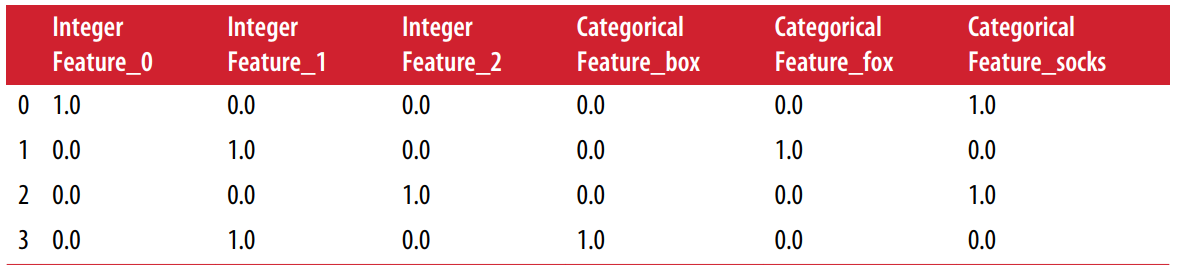
\includegraphics[scale=0.55]{Imagen_Machine/Tabla71}
		\end{tabular}
\end{table}
	
%   One-hot  instantánea 

\section{Binning, discretización, modelos lineales y árboles}
	
%	Binning, Discretization, Linear Models, and Trees

La mejor manera de representar los datos depende no sólo de la semántica de los datos, sino también del tipo de modelo que se va a utilizar.   Los modelos lineales y los  basados en árboles (como  árboles de decisión,  árboles potenciados por gradientes y  bosques aleatorios) son  dos grandes familias  muy comunes, tienen propiedades muy diferentes en cuanto a cómo funcionan con diferentes representaciones de características.  
 
Volvamos al conjunto de datos de regresión de Ondas que usamos en el capítulo \ref{Cap2}, esta  solo tiene una característica de entrada. Aquí  presentamos una comparación de un modelo de regresión lineal con  un árbol de  regresión sobre  este conjunto de datos (ver Figura \ref{Comparando01}):

	
\begin{lstlisting}%[frame=single]

In[11]:

   from sklearn.linear_model import LinearRegression
   from sklearn.tree import DecisionTreeRegressor
   
   X, y = mglearn.datasets.make_wave(n_samples=100)
   line = np.linspace(-3, 3, 1000, endpoint=False).reshape(-1, 1)
   
   reg = DecisionTreeRegressor(min_samples_split=3).fit(X, y)
   plt.plot(line, reg.predict(line), label="decision tree")
   
   reg = LinearRegression().fit(X, y)
   plt.plot(line, reg.predict(line), label="linear regression")
   plt.plot(X[:, 0], y, 'o', c='k')
   plt.ylabel("Regression output")
   plt.xlabel("Input feature")
   plt.legend(loc="best")
 
\end{lstlisting}

Como ya sabemos, los modelos lineales sólo pueden modelar relaciones lineales, que son líneas rectas en el caso de una sola característica. El árbol de decisión puede construir un modelo mucho más complejo sobre los datos. Sin embargo, esto depende fuertemente de la representación de los datos. Una manera de hacer que los modelos lineales sean más potentes en datos continuos es aplicar  {\ttfamily binning}\index{binning} (también conocido como discretización\index{discretización}) sobre la característica, para dividirla en múltiples características, como se describe a continuación.\\

\begin{figure}[h!]
	\centering
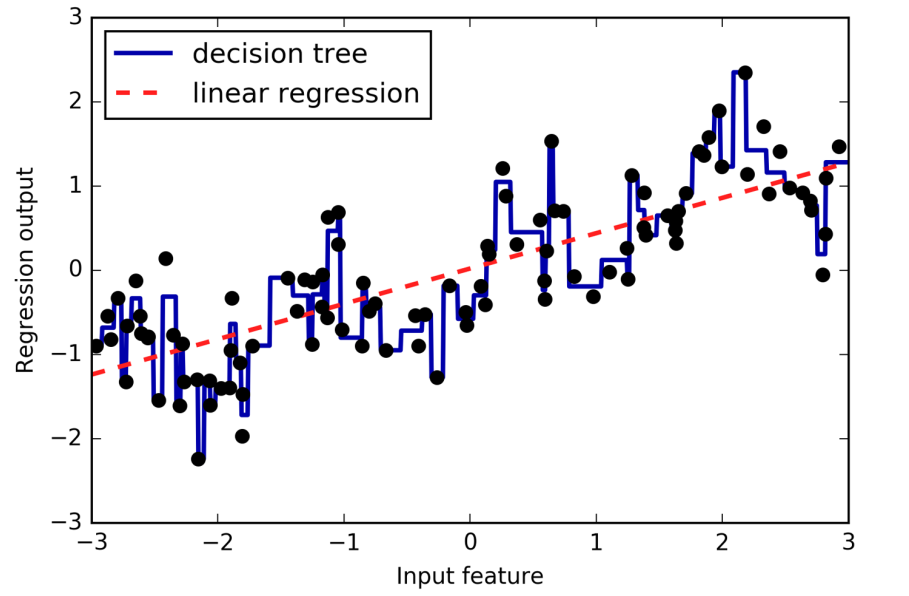
\includegraphics[scale=0.55]{Imagen_Machine/Comparando01}
	\caption{Comparación de regresión lineal y un árbol de decisión en el conjunto de datos de Onda}
	\label{Comparando01}
\end{figure}

Imaginamos una partición del rango de entrada para la característica (en este caso, los números
de –3 a 3) en un número fijo de intervalos (bins), por ejemplo 10. Un punto de datos será  representado por el intervalo que lo contenga. Para determinar esto, primero tenemos que definir los intervalos. En  este caso, definiremos 10 intervalos igualmente espaciados entre –3 y 3; utilizando la función 
{\ttfamily np.linspace}, gererando 11 entradas, que crearán 10 intervalos, que son
los espacios entre dos límites consecutivos:

\begin{lstlisting} 

In[12]:

   bins = np.linspace(-3, 3, 11)
   print("bins: {}".format(bins))

Out[12]:

    bins: [-3.  -2.4  -1.8  -1.2  -0.6  0.  0.6  1.2  1.8  2.4  3. ]

\end{lstlisting}


Aquí, el primer intervalo contiene todos los puntos de la  data con valores de características de
  \:  –3 \:    a  \:  –2.4, el segundo intervalo contiene todos los puntos con valores de características de \: –2,4 \: a \: -1.18,  y  así sucesivamente.


A continuación, registramos  cada punto de la  data en el intervalo que cae. Esto se puede calcular fácilmente usando la función {\ttfamily np.digitize}: \\


\begin{lstlisting}%[frame=single]

In[13]:

   which_bin = np.digitize(X, bins=bins)
   print("\nData points:\n", X[:5])
   print("\nBin membership for data points:\n", which_bin[:5])

Out[13]:

    Data points:
    [[-0.753]
     [ 2.704]
     [ 1.392]
     [ 0.592]
     [-2.064]]

   Bin membership for data points:
    [[ 4]
     [10]
     [ 8]
     [ 6]
     [ 2]]

\end{lstlisting}

	
Lo que hicimos aquí es transformar la característica de entrada continua única en el conjunto de datos de onda en una característica categórica que codifica en qué intervalo se encuentra un punto de datos. 

Para usar un modelo {\ttfamily scikit-learn }  sobre estos datos, transformamos esta característica discreta en una codificación one-hot,	usando el {\ttfamily OneHotEncoder} del módulo de pre-procesamiento. El {\ttfamily OneHotEncoder}  hace 	la misma codificación que {\ttfamily pandas.get\_dummies}, aunque realmente sólo actúa  sobre  variables categóricas que son enteros:\\

\begin{lstlisting}%[frame=single]

In[14]:

   from sklearn.preprocessing import OneHotEncoder
   # transform using the OneHotEncoder
   encoder = OneHotEncoder(sparse=False)
   # encoder.fit finds the unique values that appear in which_bin
   encoder.fit(which_bin)
   # transform creates the one-hot encoding
   X_binned = encoder.transform(which_bin)
   print(X_binned[:5])

Out[14]:

    [[ 0. 0. 0. 1. 0. 0. 0. 0. 0. 0.]
     [ 0. 0. 0. 0. 0. 0. 0. 0. 0. 1.]
     [ 0. 0. 0. 0. 0. 0. 0. 1. 0. 0.]
     [ 0. 0. 0. 0. 0. 1. 0. 0. 0. 0.]
     [ 0. 1. 0. 0. 0. 0. 0. 0. 0. 0.]]



\end{lstlisting}

Debido a que especificamos 10 intervalos, la data transformada {\ttfamily X\_binned} ahora se compone de 10 características:



\begin{lstlisting}%[frame=single]

In[15]:
   
   print("X_binned.shape: {}".format(X_binned.shape))

Out[15]:

    X_binned.shape: (100, 10)

\end{lstlisting}

Ahora construimos un nuevo modelo de regresión lineal y un nuevo modelo de árbol de decisión sobre la data   codificados  one-hot.   El resultado se visualiza en la Figura \ref{Comparando02}, junto con los límites  del intervalo, mostrados como líneas punteadas en negro:\\ 

\begin{lstlisting}%[frame=single]

In[16]:

   line_binned = encoder.transform(np.digitize(line, bins=bins))
   
   reg = LinearRegression().fit(X_binned, y)
   plt.plot(line, reg.predict(line_binned), label='linear regression binned')
   
   reg = DecisionTreeRegressor(min_samples_split=3).fit(X_binned, y)
   plt.plot(line, reg.predict(line_binned), label='decision tree binned')
   plt.plot(X[:, 0], y, 'o', c='k')
   plt.vlines(bins, -3, 3, linewidth=1, alpha=.2)
   plt.legend(loc="best")
   plt.ylabel("Regression output")
   plt.xlabel("Input feature")
   
\end{lstlisting}


\begin{figure}[h!]
	\centering
	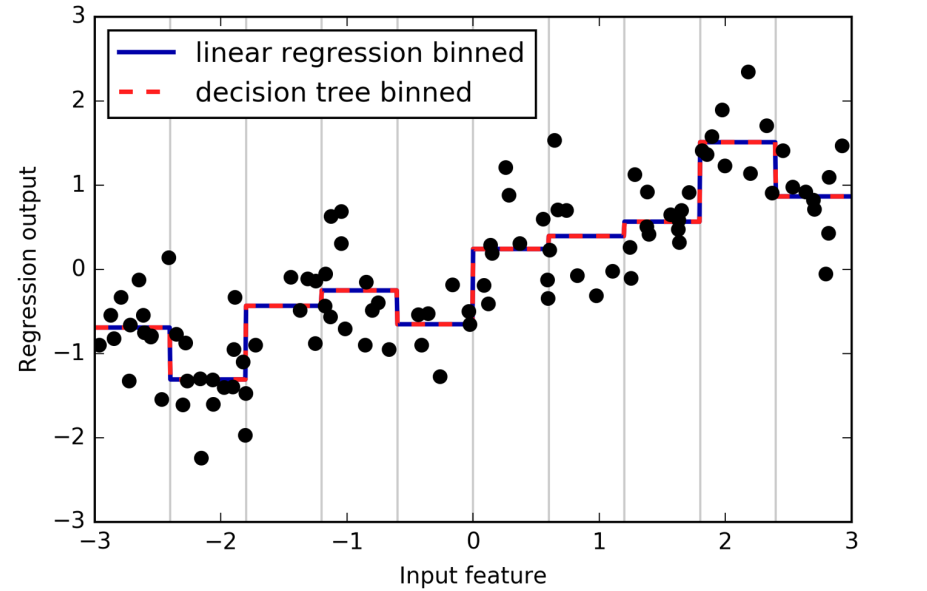
\includegraphics[scale=0.55]{Imagen_Machine/Comparando02}
	\caption{Comparación de la regresión lineal y la regresión de árbol de decisión sobre  las características en bins (agrupadas)}
	\label{Comparando02}
\end{figure}


La línea discontinua y la línea sólida están exactamente una encima de la otra, lo que significa que el modelo de regresión lineal y el árbol de decisiones hacen exactamente las mismas predicciones. Para cada intervalo, predicen un valor constante. Como las características son constantes dentro de cada intervalo, cualquier modelo debe predecir el mismo valor para todos los puntos dentro de un intervalo.

Comparando lo que los modelos aprendieron antes de combinar las características y después,
 vemos que el modelo lineal se volvió mucho más flexible, porque ahora tiene un valor diferente para cada intervalo, mientras que el modelo de árbol de decisión se volvió mucho menos flexible.
Las características  Binning generalmente no tienen ningún efecto beneficioso para los modelos basados en árboles, ya que estos modelos pueden aprender a dividir los datos en cualquier lugar. En cierto sentido, eso significa que los árboles de decisión pueden aprender lo que es más útil para predecir esta data.
 
Además, los árboles de decisión miran múltiples características a la vez, mientras que el binning generalmente se hace por cada característica. Sin embargo, el modelo lineal se benefició grandemente con la nueva transformación de los datos.\\

Si hay buenas razones para usar un modelo lineal en  un conjunto de datos en particular, por ejemplo, porque es muy grande y de alta dimensión, pero algunas características tienen relaciones no lineales, con la salida-binning puede ser una  manera de aumentar la potencia del modelo. 


\section{Interacciones y polinomios}

Otra manera de enriquecer una representación de características, particularmente para modelos lineales, es añadir  interacción de características  y  polinómicas de características a  los datos originales. Este tipo de ingeniería de características es frecuentemente usado  en el modelado estadístico, pero también es común en muchas aplicaciones prácticas de aprendizaje automático.\\

Como primer ejemplo, observe nuevamente la Figura \ref{Comparando02}. El modelo lineal aprendió un valor constante para cada intervalo en la dataset wave. Sin embargo, sabemos que los modelos lineales pueden aprender no solo las compensaciones, sino también las pendientes.
 Una forma de añadir una pendiente al modelo lineal sobre la data binned es  agregar la característica original (el eje x en la gráfica) nuevamente. Esto lleva a una dataset de  11 dimensiones, como se ve en la Figura \ref{Binned}:	
	

\begin{lstlisting}%[frame=single]

In[17]:

   X_combined = np.hstack([X, X_binned])
   print(X_combined.shape)

Out[17]:

    (100, 11)

In[18]:

   reg = LinearRegression().fit(X_combined, y)
   
   line_combined = np.hstack([line, line_binned])
   plt.plot(line, reg.predict(line_combined), 
            label='linear regression combined')
   
   for bin in bins:
       plt.plot([bin, bin], [-3, 3], ':', c='k')
       plt.legend(loc="best")
       
   plt.ylabel("Regression output")
   plt.xlabel("Input feature")
   plt.plot(X[:, 0], y, 'o', c='k')
   
\end{lstlisting}
	


\begin{figure}[h!]
	\centering
%	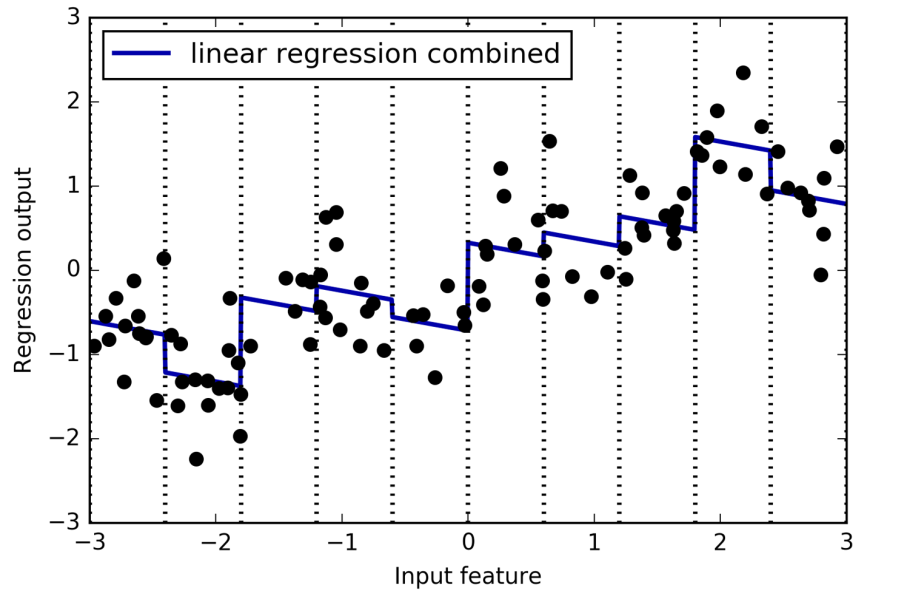
\includegraphics[scale=0.55]{Imagen_Machine/Binned}
    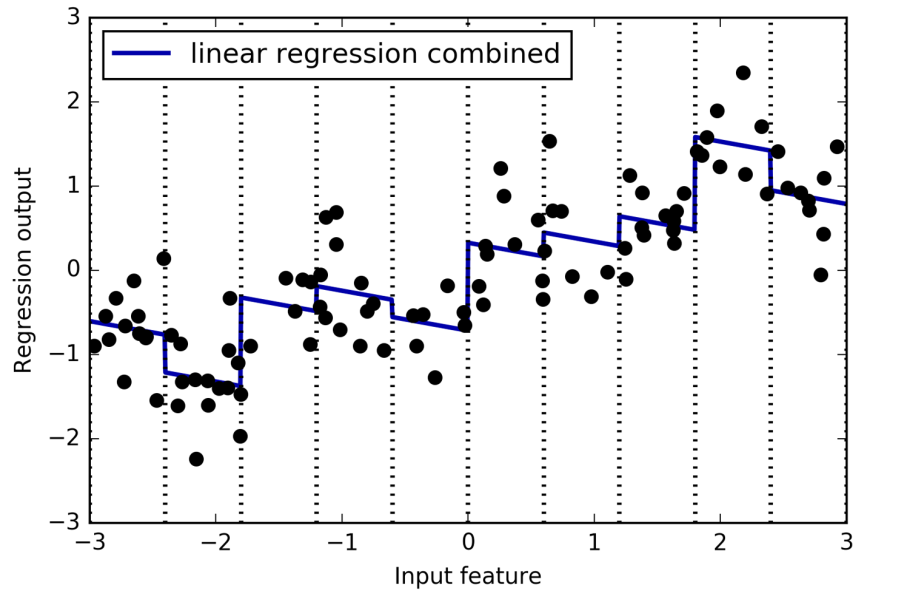
\includegraphics[scale=0.55]{Imagen_Machine/Binned}
	\caption{Regresión lineal usando características combinadas y una sola pendiente global}
	\label{Binned}
\end{figure}

En este ejemplo, el modelo aprendió una compensación  para cada intervalo, junto con una pendiente. La pendiente aprendida va hacia abajo, y se comparte a través de todos los intervalos; hay una sola característica del eje $x$, que tiene una sola pendiente. 

Debido a que la pendiente se comparte a través de todos los intervalos, no parece ser muy útil. Preferiríamos tener una pendiente separada para cada intervalo!   Podemos lograr esto añadiendo una caraterística  de interacción o producto que indica en qué intervalo se encuentra un punto de datos y dónde se encuentra en el eje x. Esta característica es un producto del intervalo indicador y de la característica original.  Vamos a crear este conjunto de datos:\\


\begin{lstlisting}%[frame=single]

In[19]:

   X_product = np.hstack([X_binned, X * X_binned])
   print(X_product.shape)

Out[19]:

    (100, 20)

\end{lstlisting}

 
La data ahora tiene 20 características: los  intervalos indicadores  en que un punto de la data está en él, y un producto de la característica original y el intervalo  indicador. Se puede pensar en el producto de la característica  como una copia separada de la característica del eje x para cada intervalo. Es la característica original dentro del intervalo, y cero en otro caso. La Figura  \ref{SeparaBin}  muestra el resultado del modelo lineal en esta nueva representación:

\begin{lstlisting}
	
In[20]:

   reg = LinearRegression().fit(X_product, y)
   
   line_product = np.hstack([line_binned, line * line_binned])
   plt.plot(line, reg.predict(line_product), 
            label='linear regression product')
   
   for bin in bins:
       plt.plot([bin, bin], [-3, 3], ':', c='k')
       
   plt.plot(X[:, 0], y, 'o', c='k')
   plt.ylabel("Regression output")
   plt.xlabel("Input feature")
   plt.legend(loc="best")


\end{lstlisting}


\begin{figure}[h!]
	\centering
	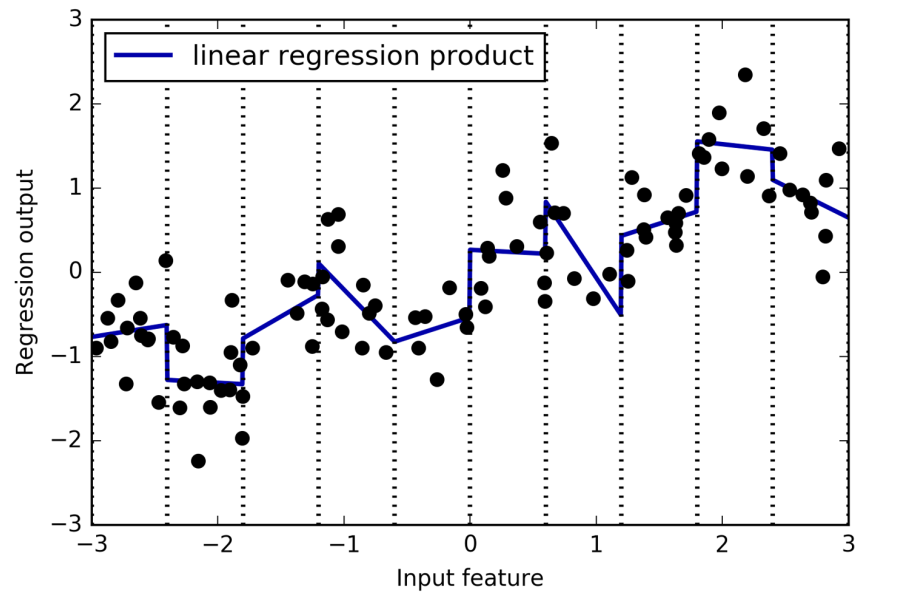
\includegraphics[scale=0.55]{Imagen_Machine/SeparaBin}
	\caption{Regresión lineal con una pendiente separada por intervalo}
	\label{SeparaBin}
\end{figure}

Como puedes ver, ahora cada intervalo  tiene su propia compensación y pendiente en este modelo.

Usar binning es una forma de expandir una característica continua. Otra es utilizar polinomios de las características originales. Para una característica dada $x$, podríamos considerar $ x**2, \: x**3, \: x**4, $ \: y así sucesivamente. Esto se implementa en {\ttfamily PolynomialFeatures} del módulo de preprocesamiento:

\begin{lstlisting}	
In[21]:

   from sklearn.preprocessing import PolynomialFeatures
   # include polynomials up to x ** 10:
   # the default "include_bias=True" adds a feature that's constantly 1
   poly = PolynomialFeatures(degree=10, include_bias=False)
   poly.fit(X)
   X_poly = poly.transform(X)
   
   
\end{lstlisting} 

El uso de  grado igual a  10, produce 10 características:

\begin{lstlisting}

In[22]:

   print("X_poly.shape: {}".format(X_poly.shape))

Out[22]:

    X_poly.shape: (100, 10)  
  
  \end{lstlisting}    
 
 Comparemos las entradas de {\ttfamily X\_poly} con las de X:\\
 
 \begin{lstlisting}%[frame=single]
 
In[23]:

   print("Entries of X:\n{}".format(X[:5]))
   print("Entries of X_poly:\n{}".format(X_poly[:5]))

Out[23]:
   
    Entries of X:
    [[-0.753]
     [ 2.704]
     [ 1.392]
     [ 0.592]
     [-2.064]]
    Entries of X_poly:
    [[    -0.753     0.567    -0.427      0.321  -0.242    0.182
          -0.137     0.103    -0.078      0.058]
    [      2.704     7.313    19.777     53.482  144.632  391.125
        1057.714  2860.360  7735.232  20918.278]
    [      1.392     1.938     2.697      3.754    5.226    7.274
          10.125    14.094    19.618     27.307]
    [      0.592     0.350     0.207      0.123    0.073    0.043
           0.025     0.015     0.009      0.005]
    [     -2.064     4.260    -8.791     18.144  -37.448   77.289
        -159.516   329.222  -679.478   1402.367]]

	



\end{lstlisting}



	Puede obtener la semántica de las características llamando al método {\ttfamily get\_feature\_names}, que proporciona el exponente para cada característica:
	
\begin{lstlisting}	
		
In[24]:

   print("Polynomial feature names:\n{}".format(poly.get_feature_names()))
   
Out[24]:
	
   Polynomial feature names:
   ['x0', 'x0^2', 'x0^3', 'x0^4', 'x0^5', 'x0^6', 'x0^7', 'x0^8', 'x0^9',
    'x0^10']
	
\end{lstlisting}
	

	
Puedes ver que la primera columna de {\ttfamily X\_poly} corresponde exactamente a X, mientras que las otras columnas son las potencias de la primera entrada. Es interesante ver lo grandes que pueden llegar a ser algunos de los valores. La segunda columna tiene entradas por encima de 20.000, órdenes de magnitud diferentes del resto. El uso de características polinómicas junto con un modelo de regresión lineal produce el modelo clásico de regresión polinómica (ver Figura \ref{Polinomio}):	

\begin{lstlisting}

In[25]:  # repetido erroe 26

   reg = LinearRegression().fit(X_poly, y)
   
   line_poly = poly.transform(line)
   plt.plot(line, reg.predict(line_poly), label='polynomial linear
            regression')
   plt.plot(X[:, 0], y, 'o', c='k')
   plt.ylabel("Regression output")
   plt.xlabel("Input feature")
   plt.legend(loc="best")

\end{lstlisting}



\begin{figure}[h!]
	\centering
	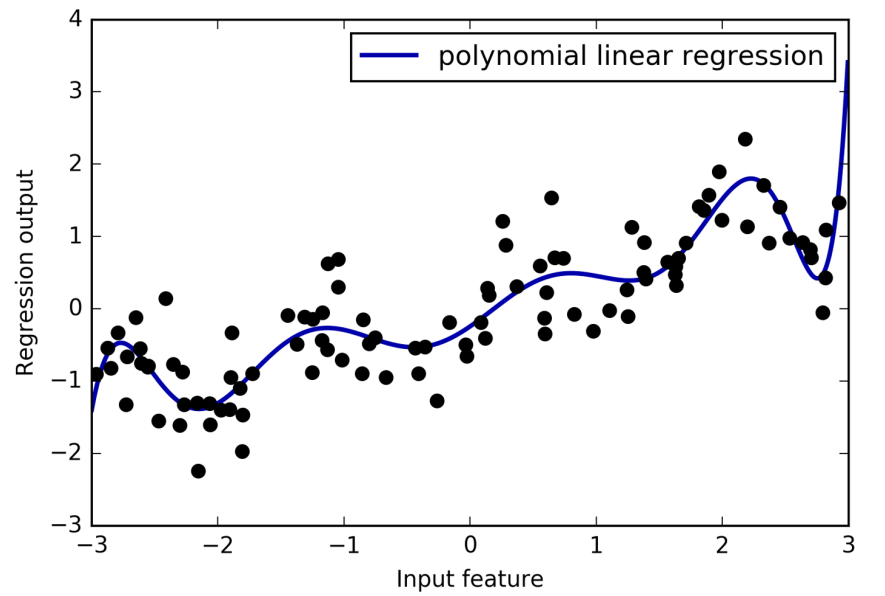
\includegraphics[scale=0.55]{Imagen_Machine/Polinomio}
	\caption{Regresión lineal con una pendiente separada por intervalo}
	\label{Polinomio}
\end{figure}


Como puedes ver, las características polinómicas producen un ajuste muy suave en estos datos unidimensionales. Sin embargo, los polinomios de alto grado tienden a comportarse de manera extrema en los límites o en regiones con pocos datos. \\

Como una comparación, aqui se presenta  un  modelo kernel SVM  aprendido sobre los datos originales, sin ninguna transformación de la data (ver Figura \ref{KernelCarat}):
	

\begin{lstlisting}

In[26]:   # error   26 repetido

  from sklearn.svm import SVR
  
  for gamma in [1, 10]:
      svr = SVR(gamma=gamma).fit(X, y)
      plt.plot(line, svr.predict(line), label='SVR gamma={}'.format(gamma))
      
  plt.plot(X[:, 0], y, 'o', c='k')
  plt.ylabel("Regression output")
  plt.xlabel("Input feature")
  plt.legend(loc="best")

  \end{lstlisting}
	
%   KernelCarat

\begin{figure}[h!]
	\centering
	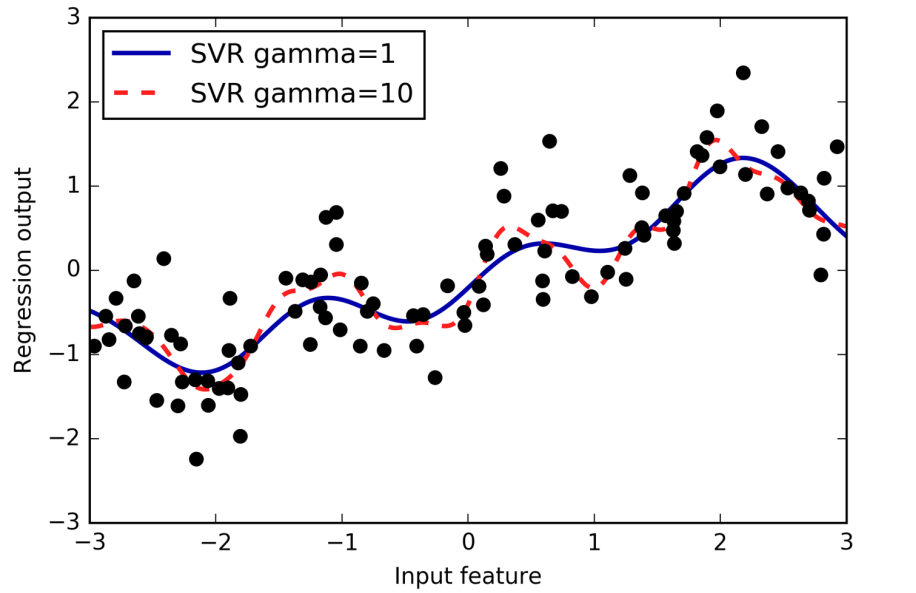
\includegraphics[scale=0.55]{Imagen_Machine/KernelCarat}
	\caption{Comparación de diferentes parámetros gamma para un SVM con el núcleo RBF}
	\label{KernelCarat}
\end{figure}


Usando un modelo más complejo, un SVM kernel, podemos aprender una predicción igualmente compleja de la regresión polinómica sin una transformación explícita de las características.


Como una aplicación más realista de interacciones y polinomios, veamos de nuevo el conjunto de datos de Boston Housing. Ya hemos utilizado características polinómicas sobre  este conjunto de datos en el capítulo \ref{Cap2}.  Ahora veamos cómo se construyeron estas características, y en qué medida las características polinómicas ayudan. Primero cargamos los datos y los reescalemos  entre 0 y 1 usando {\ttfamily MinMaxScaler}: \\	

 
\begin{lstlisting}%[frame=single]

In[27]:

   from sklearn.datasets import load_boston
   from sklearn.model_selection import train_test_split
   from sklearn.preprocessing import MinMaxScaler
   
   boston = load_boston()
   X_train, X_test, y_train, y_test = train_test_split(
        boston.data, boston.target, random_state=0)
       
   # rescale data
   scaler = MinMaxScaler()
   X_train_scaled = scaler.fit_transform(X_train)
   X_test_scaled = scaler.transform(X_test)

\end{lstlisting}


Ahora, extraemos características e interacciones polinómicas hasta el grado de 2:\\


\begin{lstlisting}%[frame=single]

In[28]:

   poly = PolynomialFeatures(degree=2).fit(X_train_scaled)
   X_train_poly = poly.transform(X_train_scaled)
   X_test_poly = poly.transform(X_test_scaled)
   print("X_train.shape: {}".format(X_train.shape))
   print("X_train_poly.shape: {}".format(X_train_poly.shape))

Out[28]:

   X_train.shape: (379, 13)
   X_train_poly.shape: (379, 105)


\end{lstlisting}%[frame=single]

 
Los datos originalmente tenían 13 características, que se ampliaron en 105 características  de interacción. Estas nuevas características representan todas las interacciones posibles entre dos características originales y por supuesto diferentes, así como el cuadrado de cada característica original. El grado 2 (degree = 2)   significa que miramos todas las características que son el producto de  dos características originales. La correspondencia exacta entre las características de entrada y salida se puede encontrar usando el método {\ttfamily get\_feature\_names}:\\

\begin{lstlisting}  %[frame=single]

In[29]:

   print("Polynomial feature names:\n{}".format(poly.get_feature_names()))

Out[29]:

   Polynomial feature names:
   ['1', 'x0', 'x1', 'x2', 'x3', 'x4', 'x5', 'x6', 'x7', 'x8', 'x9', 'x10',
   'x11', 'x12', 'x0^2', 'x0 x1', 'x0 x2', 'x0 x3', 'x0 x4', 'x0 x5', 
   'x0 x6','x0 x7', 'x0 x8', 'x0 x9', 'x0 x10', 'x0 x11', 'x0 x12', 'x1^2',
   'x1 x2','x1 x3', 'x1 x4', 'x1 x5', 'x1 x6', 'x1 x7', 'x1 x8', 'x1 x9', 
   'x1 x10','x1 x11', 'x1 x12', 'x2^2', 'x2 x3', 'x2 x4', 'x2 x5', 'x2 x6',
   'x2 x7', 'x2 x8', 'x2 x9', 'x2 x10', 'x2 x11', 'x2 x12', 'x3^2', 'x3 x4',
   'x3 x5', 'x3 x6', 'x3 x7', 'x3 x8', 'x3 x9', 'x3 x10', 'x3 x11', 'x3 x12', 
   'x4^2',  'x4 x5', 'x4 x6', 'x4 x7', 'x4 x8', 'x4 x9', 'x4 x10', 'x4 x11', 
   'x4 x12', 'x5^2', 'x5 x6', 'x5 x7', 'x5 x8', 'x5 x9', 'x5 x10', 'x5 x11', 
   'x5 x12', 'x6^2', 'x6 x7', 'x6 x8', 'x6 x9', 'x6 x10', 'x6 x11', 'x6 x12', 
   'x7^2', 'x7 x8', 'x7 x9', 'x7 x10', 'x7 x11', 'x7 x12', 'x8^2', 'x8 x9', 
   'x8 x10', 'x8 x11', 'x8 x12', 'x9^2', 'x9 x10', 'x9 x11', 'x9 x12',
    'x10^2', 'x10 x11', 'x10 x12', 'x11^2', 'x11 x12', 'x12^2']


\end{lstlisting}

La primera característica nueva es una característica constante, llamada "1".  Las siguientes 13 características son las características originales (llamadas "x0"{}  a "x12"). Luego sigue la primera característica al cuadrado ("x0\^{}2") y las combinaciones de la primera y con las demás características. \\

Comparemos el rendimiento usando Ridge en los datos con y sin interacciones:\\



\begin{lstlisting}%[frame=single]

In[30]:

   from sklearn.linear_model import Ridge
   ridge = Ridge().fit(X_train_scaled, y_train)
   print("Score without interactions: {:.3f}".format(
          ridge.score(X_test_scaled, y_test)))
   ridge = Ridge().fit(X_train_poly, y_train)
   print("Score with interactions: {:.3f}".format(
          ridge.score(X_test_poly, y_test)))

Out[30]:

    Score without interactions: 0.621
    Score with interactions: 0.753

\end{lstlisting}

Claramente, las interacciones y características polinómicas nos dieron un buen impulso en el rendimiento cuando se utiliza Ridge.  Aunque cuando se utiliza un modelo más complejo como un bosque aleatorio, la historia es un poco diferente, veamos en el siguiente ejemplo:


\begin{lstlisting}%[frame=single]


In[31]:

   from sklearn.ensemble import RandomForestRegressor
   rf = RandomForestRegressor(n_estimators=100).fit(X_train_scaled, y_train)
   print("Score without interactions: {:.3f}".format(
       rf.score(X_test_scaled, y_test)))
   rf = RandomForestRegressor(n_estimators=100).fit(X_train_poly, y_train)
   print("Score with interactions: {:.3f}".format(
           rf.score(X_test_poly, y_test)))

Out[31]:

    Score without interactions: 0.799
    Score with interactions: 0.763

\end{lstlisting}

Se puede ver que incluso sin características adicionales, el bosque aleatorio supera el rendimiento de Ridge. Añadiendo interacciones y polinomios disminuye ligeramente el rendimiento. 

\section{Transformaciones  univariables  no lineales}

Acabamos de ver que agregando características al cuadradas  o al cubo puede ayudar con 
los modelos lineales para  regresión. Hay otras transformaciones que a menudo resultan útiles para transformar ciertas características:  en particular, la aplicación de funciones matemáticas como $log,\: exp $  o $ \: sin$.  Mientras que en los modelos basados en árboles sólo  preocupa  el orden de las características, en los modelos lineales y las redes neuronales están muy ligadas a la escala y distribución de cada característica, y si existe es una relación no lineal entre la característica y el objetivo, se hace más difícil  modelar, particularmente en el caso de regresión. 
Las funciones  $log $  y  $ exp$  pueden ayudar ajustando las escalas relativas sobre los datos para que puedan ser capturados mejor por un modelo lineal o red neuronal. 
 
En el Capítulo \ref{Cap2} vimos una aplicación de esta técnica sobre los datos de precio de memoria RAM. Los
Las funciones $ sin $ y $ cos $ pueden ser útiles cuando se trata de datos que codifican patrones  periódicos.\\

La mayoría de los modelos funcionan mejor cuando cada característica (y en regresión también el objetivo) está distribuida vagamente gaussiana, es decir, un histograma de cada característica debe tener algo parecido a la familiar forma de "{}curva de campana". 
Usar transformaciones como $log$  y  $ exp$  es una forma simple y eficiente de lograr esto. Un caso particularmente común cuando tal transformación puede ser útil es cuando se trata de datos de recuento entero.  Por datos de recuento, nos referimos a características como "{}¿ Con qué frecuencia el usuario A inicia sesión ?"{}. Los recuentos nunca son negativos, y a menudo siguen patrones estadísticos particulares. Estamos utilizando una data sintética de conteos que tiene propiedades similares a las que se pueden encontrar en la naturaleza. Las características son todas de valor entero, mientras que la respuesta es continua:\\


\begin{lstlisting}%[frame=single]

In[32]:

   rnd = np.random.RandomState(0)
   X_org = rnd.normal(size=(1000, 3))
   
   w = rnd.normal(size=3)
   X = rnd.poisson(10 * np.exp(X_org))
   y = np.dot(X_org, w)

\end{lstlisting}


Veamos las primeras 10 entradas de la primera característica. Todos son valores enteros y positivos, pero aparte de eso es difícil distinguir un patrón particular. Si contamos la apariencia de cada valor, la distribución de valores se vuelve más clara:\\

\begin{lstlisting}%[frame=single]

In[33]:

   print("Number of feature appearances:\n{}".format(np.bincount(X[:, 0])))

Out[33]:
 
    Number of feature appearances:
    [28 38 68 48 61 59 45 56 37 40 35 34 36 26 23 26 27 21 23 23 18 21 10  9 
     17  9  7 14 12  7  3  8  4  5  5  3  4  2  4  1  1  3  2  5  3  8  2  5 
      2  1  2  3  3  2  2  3  3  0  1  2  1  0  0  3  1  0  0  0  1  3  0  1 
      0  2  0  1  1  0  0  0  0  1  0  0  2  2  0  1  1  0  0  0  0  1  1  0
      0  0  0  0  0  0  1  0  0  0  0  0  1  1  0  0  1  0  0  0  0  0  0  0
      1  0  0  0  0  1  0  0  0  0  0  0  0  0  0  0  0  0  0  0  1]
\end{lstlisting}

El valor 2 parece ser el más común, con 68 apariencias (el conteo siempre comienza en 0), y el conteo de valores más altos cae rápidamente. Sin embargo, hay algunos valores muy altos, como 134 apareciendo dos veces. Podemos visualizamos los conteos en la Figura \ref{HistoValores}:\\

\begin{lstlisting}%[frame=single]

In[34]:

   bins = np.bincount(X[:, 0])
   plt.bar(range(len(bins)), bins, color='w')
   plt.ylabel("Number of appearances")
   plt.xlabel("Value")

\end{lstlisting}


\begin{figure}[h!]
	\centering
	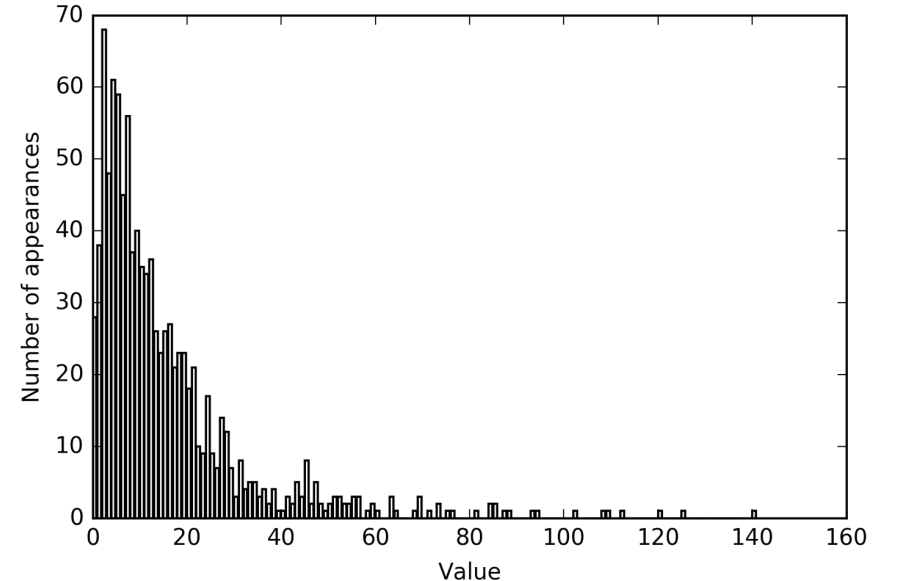
\includegraphics[scale=0.55]{Imagen_Machine/HistoValores}
	\caption{Histograma de los valores de las características de X[0]}
	\label{HistoValores}
\end{figure}

                       %                              \tiny
Las características  X[:, 1]  y  X[:, 2]  tienen propiedades similares. Este tipo de distribución de valores (muchos valores  muy pequeños y pocos muy grandes) es muy común en la práctica{\footnote{\scriptsize	{ Esta es una distribución de Poisson, que es bastante fundamental para contar datos}}}. Sin embargo, es algo que la mayoría de los modelos lineales no pueden manejar muy bien. Vamos a tratar de encajar una regresión  Ridge a este modelo:\\


\begin{lstlisting}%[frame=single]

In[35]:

   from sklearn.linear_model import Ridge
   X_train, X_test, y_train, y_test = train_test_split(X, y, random_state=0)
   score = Ridge().fit(X_train, y_train).score(X_test, y_test)
   print("Test score: {:.3f}".format(score))

Out[35]:

    Test score: 0.622

\end{lstlisting}


Como se puede ver  la puntuación $R^{2}$ relativamente baja, Ridge no fue capaz de capturar realmente la relación entre $X$ e $y$. Sin embargo, aplicando  una transformación logarítmica puede ayudar.  Debido a que el valor 0 aparece en la data (y el logaritmo no está definido en 0), no podemos aplicar $log$, pero tenemos que calcular $log(X + 1)$:\\


\begin{lstlisting}%[frame=single]

In[36]:

   X_train_log = np.log(X_train + 1)
   X_test_log = np.log(X_test + 1)
\end{lstlisting}


Después de la transformación, la distribución de los datos es menos asimétrica y  no tiene valores atípicos (outliers) tan  grandes (ver Figura \ref{HistoValores2}):\\
 
 
\begin{lstlisting}%[frame=single]

In[37]:

   plt.hist(np.log(X_train_log[:, 0] + 1), bins=25, color='gray')
   plt.ylabel("Number of appearances")
   plt.xlabel("Value")
\end{lstlisting}


\begin{figure}[h!]
	\centering
	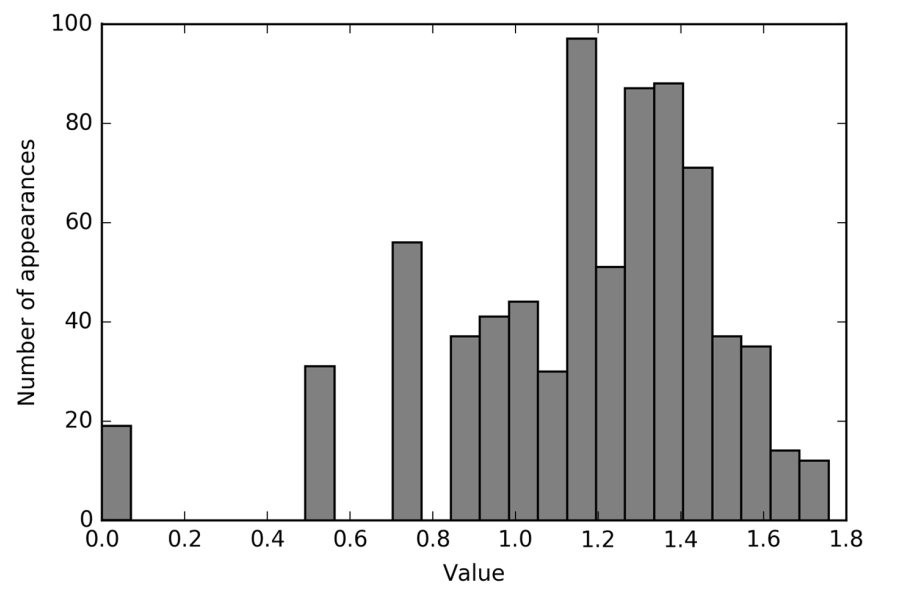
\includegraphics[scale=0.55]{Imagen_Machine/HistoValores2}
	\caption{Histograma de los valores de las características para X[0] después de la transformación logarítmica}
	\label{HistoValores2}
\end{figure}

La construcción de un modelo Ridge sobre  la data nueva  proporciona un ajuste mucho mejor:\\

\begin{lstlisting}%[frame=single]

In[38]:

   score = Ridge().fit(X_train_log, y_train).score(X_test_log, y_test)
   print("Test score: {:.3f}".format(score))

Out[38]:
   
    Test score: 0.875
\end{lstlisting}



Encontrar la transformación que funciona mejor para cada combinación de dataset y modelo es  un arte. En este ejemplo, todas las características tenían las mismas propiedades.  En la práctica esto se presenta raramente, y por lo general sólo un subconjunto de las características debe ser transformado, o a veces cada característica tiene que ser transformado de una manera diferente.   Como mencionamos anteriormente, este tipo de transformaciones son irrelevantes para los modelos basados en árboles, pero podrían ser esenciales para los modelos lineales.  A veces también es una buena idea transformar la variable objetivo $y$ en regresión. Tratar de predecir los conteos (por ejemplo, el número de órdenes) es una tarea muy común, y usar la transformación $ log(y + 1)$ a menudo ayuda{\footnote{\scriptsize Esta es una aproximación muy cruda del uso de la regresión de Poisson, que sería la solución adecuada desde un punto de vista probabilístico}}.\\

Como vieron en los ejemplos anteriores, el binning, los polinomios y las interacciones pueden tener una gran influencia en cómo funcionan los modelos en un conjunto de datos dado. 
 Esto es particularmente cierto para los modelos menos complejos como los modelos lineales y los modelos   naives Bayes. Por otra parte, los modelos basados en árboles,  a menudo son capaces de descubrir interacciones importantes, y no requieren la transformación explícitamente de los datos en la mayor parte de las veces.   Otros modelos, como   SVMs,  vecinos más cercanos  y  redes neuronales, a veces podrían beneficiarse del uso de binning, interacciones o polinomios, pero las implicaciones allí son generalmente mucho menos claras que en el caso de los modelos lineales.


\section{Selección automática de características}

Con tantas formas de crear nuevas características, puede sentirse tentado a aumentar la dimensionalidad de los datos más allá del número de características originales.  Sin embargo, agregar más características  hace que todos los modelos sean más complejos,  y  por lo tanto, aumenta la posibilidad de sobreajuste. Al agregar nuevas características o en caso de datas con alta dimensión,   puede ser una buena idea reducir la cantidad de características  solo a las más útiles, y descartar el resto. Esto puede conducir a modelos más simples que generalizan mejor. Pero  ¿ cómo se puede saber qué tan importante es una  característica?   Hay tres estrategias básicas: las estadísticas  univariante, la selección basada en modelos y la selección iterativa. Discutiremos los tres en detalle. Todos estos son métodos  supervisados, lo que significa que necesitan un objetivo para ajustar el modelo. Esto significa que necesitamos dividir los datos en entrenamiento y prueba, y   ajustar  la selección de características sólo en la parte de la  data de  entrenamiento.

\subsubsection{Estadísticas univariada}

En las estadísticas univariantes  calculamos si existe una relación estadísticamente significativa  entre cada característica y el objetivo. Luego, se seleccionan las características que se relacionan con la mayor confianza. En el caso de la clasificación,  esto también se conoce como
Análisis de Varianza (ANOVA). Una propiedad clave de estas pruebas es que son univariadas, lo que significa que sólo se considera cada característica en foma individual.  En consecuencia, una característica se descartará si sólo es informativo cuando se combina con otra característica.  Las pruebas univariadas suelen ser muy rápidas de calcular y no requieren la construcción de un modelo. Por otro lado, son completamente independientes del modelo que se desea aplicar después de la selección de características.\\

Para usar la selección de características univariadas en {\ttfamily scikit-learn}, debe elegir una prueba,  \:  generalmente  para clasificación  \:  {\ttfamily f\_classif} \: (por defecto)  y  para regresión  {\ttfamily f\_regression}, y un método para descartar características basadas en los $p$-valoes  determinados en la prueba.  Todos los métodos para descartar parámetros usan un umbral para descartar todas las características con  un $p$-valor alto (lo que significa que es poco probable que estén relacionados con el objetivo). Los métodos  difieren en cómo calculan este umbral, siendo los más simples {\ttfamily SelectKBest}, que selecciona un número fijo  de $k$  características, y el {\ttfamily SelectPercentile}, que selecciona  un porcentaje fijo de características. Apliquemos la selección de características para clasificación sobre la  cancer dataset. Para hacer la tarea un poco más difícil, añadiremos algunas características de ruido no informativa a los datos. Esperamos que la selección de características sea capaz de identificar las características que no son informativas y eliminarlas:


\begin{lstlisting}%[frame=single]

In[39]:

   from sklearn.datasets import load_breast_cancer
   from sklearn.feature_selection import SelectPercentile
   from sklearn.model_selection import train_test_split
   
   cancer = load_breast_cancer()
   
   # get deterministic random numbers
   rng = np.random.RandomState(42)
   noise = rng.normal(size=(len(cancer.data), 50))
   # add noise features to the data
   # the first 30 features are from the dataset, the next 50 are noise
   X_w_noise = np.hstack([cancer.data, noise])
   
   X_train, X_test, y_train, y_test = train_test_split(
       X_w_noise, cancer.target, random_state=0, test_size=.5)
   # use f_classif (the default) and SelectPercentile to select 
   # 50% of features 
   select = SelectPercentile(percentile=50)
   select.fit(X_train, y_train)
   # transform training set
   X_train_selected = select.transform(X_train)

   print("X_train.shape: {}".format(X_train.shape))
   print("X_train_selected.shape: {}".format(X_train_selected.shape))

Out[39]:

    X_train.shape: (284, 80)
    X_train_selected.shape: (284, 40)

\end{lstlisting}


Como se puede ver, el número de características se redujo de  80  a  40 (50 por ciento del número original de características). Podemos averiguar qué características se han seleccionado utilizando el método {\ttfamily get\_support}, que devuelve una máscara booleana de las características seleccionadas (visualizada en la Figura \ref{SelecioPercet}):




\begin{lstlisting}%[frame=single]

In[40]:

   mask = select.get_support()
   print(mask)
   # visualize the mask -- black is True, white is False
   plt.matshow(mask.reshape(1, -1), cmap='gray_r')
   plt.xlabel("Sample index")

Out[40]:

    [ True True True True True True True True True False True False
      True True True True True True False False True True True True
      True True True True True True False False False True False True
      False False True False False False False True False False True False
      False True False True False False False False False False True False
      True False False False False True False True False False False False
      True True False True False False False False]


\end{lstlisting}




\begin{figure}[h!]
	\centering
	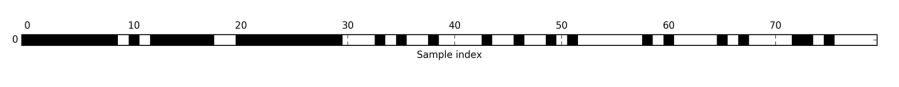
\includegraphics[scale=0.55]{Imagen_Machine/SelecioPercet}
	\caption{Características seleccionadas por SelectPercentile}
	\label{SelecioPercet}
\end{figure}



Como se puede ver en la visualización de la máscara, la mayoría de las características seleccionadas son las características originales, y la mayoría de las características de ruido se eliminaron. Sin embargo, 
la recuperación de las características originales no es perfecta. Vamos a comparar el rendimiento de la regresión logística en todas las características contra el rendimiento utilizando sólo las características seleccionadas:


\begin{lstlisting}%[frame=single]

In[41]:

   from sklearn.linear_model import LogisticRegression
   
   # transform test data
   X_test_selected = select.transform(X_test)
   
   lr = LogisticRegression()
   lr.fit(X_train, y_train)
   print("Score with all features: {:.3f}".format(lr.score(X_test, y_test)))
   lr.fit(X_train_selected, y_train)
   print("Score with only selected features: {:.3f}".format(
       lr.score(X_test_selected, y_test)))

Out[41]:

    Score with all features: 0.930
    
\end{lstlisting}

En este caso, la eliminación de las características de ruido mejoró el rendimiento, aunque algunos
de las características originales se perdieron. Este fue un ejemplo sintético  simple, y los resultados en datos reales suelen ser mixtos.

La selección de características univariadas puede ser muy útil, sin embargo, si hay un gran número de características que crean un modelo,  entonces no es factible, o si se sospecha que muchas características  son completamente {\bf{no} } informativas.

\subsection{Selección de características basada en modelos}

 La selección de características basada en un  modelo usa un modelo de aprendizaje automático supervisado para juzgar la  importancia de cada característica, y conserva solo las más importantes. 
 El modelo supervisado  que se usa para la selección de características  no necesita ser el mismo modelo que se usa para el modelo supervisado final.   El modelo de selección de características debe proporcionar alguna medida de importancia para cada característica, para que puedan ser clasificadas.

 Los árboles de decisión y los modelos basados árbol de decisión proporcionan un atributo  {\ttfamily feature\_importances\_}, que codifica directamente la importancia de cada característica.   Los modelos lineales tienen coeficientes, que también  pueden ser usados  para capturar las importancias de características considerando los valores absolutos.   Como vimos en el capítulo \ref{Cap2}, los modelos lineales con penalización L1 el aprendizaje de los  coeficientes sparse, que sólo utilizan un pequeño subconjunto de características.   Esto se puede ver como una forma de selección de características para el propio modelo, pero también se puede utilizar como un paso de preprocesamiento para seleccionar características para otro modelo. 
 En contraste con la selección univariable, la selección basada en modelos considera todas las características a la vez, y así puede capturar interacciones (si el modelo puede capturarlas).
 
  Para usar la selección de características basada en modelos, necesitamos usar el transformador {\ttfamily SelectFromModel}:\\


\begin{lstlisting}%[frame=single]

In[42]:
 
   from sklearn.feature_selection import SelectFromModel
   from sklearn.ensemble import RandomForestClassifier
   select = SelectFromModel(
            RandomForestClassifier(n_estimators=100, random_state=42),
            threshold="median")
       
\end{lstlisting}

La clase {\ttfamily SelectFromModel} selecciona todas las características que tienen una medida de importancia de la característica (según lo dispuesto por el modelo supervisado) mayor que el umbral proporcionado.  Para obtener un resultado comparable a lo que obtuvimos con la selección de características univariadas, utilizamos la mediana como un umbral, de modo que se seleccionará la mitad de las características.  Utilizamos un clasificador de bosques aleatorio con 100 árboles para calcular la importancia de las características. Este es un modelo muy  complejo y mucho más potente que el uso de pruebas univariadas. 
 


Ahora ajustemos el modelo:\\


\begin{lstlisting}%[frame=single]

In[43]:

   select.fit(X_train, y_train)
   X_train_l1 = select.transform(X_train)
   print("X_train.shape: {}".format(X_train.shape))
   print("X_train_l1.shape: {}".format(X_train_l1.shape))

Out[43]:
   
   X_train.shape: (284, 80)
   X_train_l1.shape: (284, 40)
   
\end{lstlisting}


Una vez más, podemos ver las características que fueron seleccionados (Figura \ref{SelecioPercet2}):

\begin{lstlisting}

In[44]:

   mask = select.get_support()
   # visualize the mask -- black is True, white is False
   plt.matshow(mask.reshape(1, -1), cmap='gray_r')
   plt.xlabel("Sample index")
   
\end{lstlisting}


\begin{figure}[h!]
	\centering
	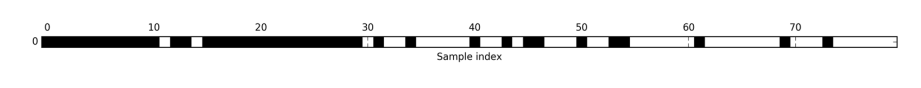
\includegraphics[scale=0.55]{Imagen_Machine/SelecioPercet2}
	\caption{Características seleccionadas por {\ttfamily SelectFromModel} usando el  {\ttfamily  RandomForestClassifier}}
	\label{SelecioPercet2}
\end{figure}


Esta vez, todas menos dos de las características originales fueron seleccionadas. Debido a que especificamos  40 características a seleccionar, algunas de las características de ruido también se seleccionaron. Veamos el rendimiento o desempeño:\\

\begin{lstlisting}%[frame=single]

In[45]:

   X_test_l1 = select.transform(X_test)
   score = LogisticRegression().fit(X_train_l1, y_train).score(X_test_l1,
                                                                y_test)
   print("Test score: {:.3f}".format(score))

Out[45]:
    
    Test score: 0.951

\end{lstlisting}

Con la mejor selección de característica, también hemos ganado algunas mejoras aquí.

\subsubsection{Selección iterativa de características}

En las pruebas univariates no usamos ningún modelo, mientras que en la selección basada en modelo
usamos un solo modelo  para seleccionar características. Ahora para la  selección iterativa de características, se construyen una serie de modelos, con un número variable de características. 

 Hay dos métodos básicos: comenzar sin características y agregando características una por una hasta que se alcance algún criterio de parada, o comenzando con todas las características y eliminar las características una por una hasta que se detenga por algún criterio de parada.   Debido a que se construyen una serie de modelos, estos métodos son mucho más  costoso computacionalmente  que los métodos que discutimos anteriormente. Un método  particular de este tipo es la eliminación recursiva de características (RFE, recursive feature elimination), que comienza 
 con todas las  características, crea un modelo y descarta la característica menos importante de acuerdo con el modelo.  Luego se construye un nuevo modelo utilizando todas las 
 características excepto las descartadas, y así sucesivamente hasta sólo queda un número pre-especificado de características. Para que esto funcione, el modelo usado para la selección debe proporcionar alguna forma de determinar la importancia de la característica, como fue el caso de la selección basada en el modelo. 

Aquí, usamos el mismo modelo de bosque aleatorio que empleamos anteriormente,  los resultados obtenidos
se muestran en la Figura \ref{SelecioPercet3}:


\begin{lstlisting}%[frame=single]

In[46]:

   from sklearn.feature_selection import RFE
   select = RFE(RandomForestClassifier(n_estimators=100, random_state=42),
                n_features_to_select=40)
                
   select.fit(X_train, y_train)
   # visualize the selected features:
   mask = select.get_support()
   plt.matshow(mask.reshape(1, -1), cmap='gray_r')
   plt.xlabel("Sample index")

\end{lstlisting}



\begin{figure}[h!]
	\centering
	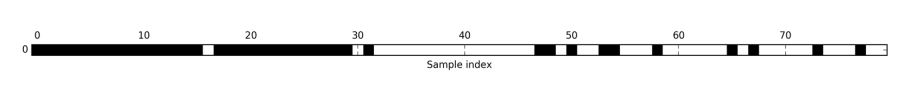
\includegraphics[scale=0.55]{Imagen_Machine/SelecioPercet3}
	\caption{Características seleccionadas por eliminación de características recursivas 
		con el modelo de clasificador bosques aleatorio}
	\label{SelecioPercet3}
\end{figure}

La selección de las características mejoró en comparación con la selección univariable y basada en modelos, pero una de las características todavía se perdió. Ejecutando  este código también toma mucho más tiempo que la selección basada en modelos, porque un modelo de bosque aleatorio se entrena 40 veces, una vez por cada característica que se elimina. 

Vamos a probar la precisión del modelo de regresión logística cuando se utiliza RFE para la selección de características:\\


\begin{lstlisting}%[frame=single]

In[47]:

   X_train_rfe= select.transform(X_train)
   X_test_rfe= select.transform(X_test)
   
   score = LogisticRegression().fit(X_train_rfe, y_train).score(X_test_rfe, y_test)
   print("Test score: {:.3f}".format(score))

Out[47]:

    Test score: 0.951

\end{lstlisting}


También podemos usar el modelo usado dentro del RFE para hacer predicciones. Esto usa sólo el conjunto de características que fue seleccionado:\\

\begin{lstlisting}%[frame=single]

In[48]:

   print("Test score: {:.3f}".format(select.score(X_test, y_test)))

Out[48]:

    Test score: 0.951


\end{lstlisting}


Aquí, el rendimiento del bosque aleatorio utilizado dentro del RFE es el mismo que se
logró entrenando un modelo de regresión logística sobre las características seleccionadas. En
en otras palabras, una vez que hemos seleccionado las características correctas, el modelo lineal funciona  también  como el bosque aleatorio.\\

 Si no está seguro qué características  seleccionar  como entrada para sus algoritmos de aprendizaje automático, la selección automática de características puede ser muy útil.  También es ideal para reducir la cantidad de características  necesarias, por ejemplo, para acelerar  la predicción o permitir modelos más interpretables. En la mayoría de los casos del mundo real,  la aplicación de selección de características es  poco probable que proporcione grandes ganancias en el rendimiento. Sin embargo, sigue siendo una herramienta valiosa en la caja de herramientas  del ingeniero de características.
   

\section{Utilizando conocimiento experto}


La ingeniería de características es a menudo un lugar importante para utilizar el conocimiento experto a una   aplicación particular. Si bien el propósito del aprendizaje automático en muchos casos es evitar
 crear un conjunto de reglas diseñadas por expertos, eso no significa que el conocimiento previo de
la aplicación o dominio debe descartarse.

Con frecuencia, los expertos en el área o experiencias  pueden ayudar en identificar características
útiles que son mucho más informativas que la representación inicial 
de la data.  Imagina que trabajas para una agencia de viajes y quieres predecir los precios de vuelo. 
Supongamos que tiene un registro de precios de diferentes  aerolíneas con fechas, lugar de salida
y destinos. Un modelo de aprendizaje automático podría ser capaz de construir un buen  modelo  a partir de estos datos.  Sin embargo, algunos factores importantes en los precios de los vuelos no se pueden aprender.
Por ejemplo, los vuelos suelen ser más caros durante los meses pico de vacaciones y
alrededor de los días festivos.
Si bien las fechas de algunos días festivos (como Navidad) son fijas, y
su efecto, por lo tanto, se puede aprender a partir de la fecha, otros pueden depender de las fases
de la luna (como los días de Hanukkah y Pascua) o ser establecido por las autoridades (como las vacaciones escolares). Estos eventos no  pueden  ser  aprendidos de la data si cada vuelo sólo se registra
usando la fecha (Gregoriana).  Sin embargo, es fácil agregar una característica  que codifique si un
el vuelo fue antes o después de un feriado público o escolar. 
De esta manera, el conocimiento previo sobre la naturaleza de la tarea se puede codificar en características para ayudar al algoritmo de aprendizaje automático.
 Agregar características no obliga a un algoritmo de aprendizaje automático a usarlo, e incluso si la información de vacaciones resulta no ser informativa  para los precios de los vuelos, aumentar los datos con esta información no hace daño. \\
 
 
Ahora veremos un caso particular de uso de conocimiento experto, aunque en este caso
podría llamarse más legítimamente "{}sentido común"{}.  La tarea es predecir el alquiler de bicicletas frente a la casa de Andreas.\\


En Nueva York, Citi Bike opera una red de estaciones de alquiler de bicicletas con un sistema de  suscripción.  Las estaciones están por toda la ciudad y proporcionan una manera conveniente de llegar
alrededor. Los datos de alquiler de bicicletas se hacen públicos de forma anónima y se han analizado de varias maneras.   La tarea que queremos resolver es predecir   cuántas personas alquilarán una bicicleta frente a la casa de Andreas en una hora y un día determinado, conociendo si hay alguna persona interesada  se le dejarán bicicletas.   Primero cargamos los datos de agosto de 2015 para esta estación en particular como una {\ttfamily Data Frame} de  {\ttfamily pandas}. Remuestreamos la data en intervalos de tres horas para obtener las principales tendencias por cada día:\\

\begin{lstlisting}%[frame=single]

In[49]:

   citibike = mglearn.datasets.load_citibike()


In[50]:

   print("Citi Bike data:\n{}".format(citibike.head()))

Out[50]:

    Citi Bike data:
    starttime
    2015-08-01 00:00:00 3.0
    2015-08-01 03:00:00 0.0
    2015-08-01 06:00:00 9.0
    2015-08-01 09:00:00 41.0
    2015-08-01 12:00:00 39.0
    Freq: 3H, Name: one, dtype: float64

\end{lstlisting}

El siguiente ejemplo muestra una visualización de las frecuencias de alquiler para todo el mes (Figura \ref{Bike1}):\\
   %     marca de tiempo de Unix 

\begin{lstlisting}%[frame=single]

In[51]:

   plt.figure(figsize=(10, 3))
   xticks = pd.date_range(start=citibike.index.min(), 
                           end=citibike.index.max(), freq='D')
   plt.xticks(xticks, xticks.strftime("%a %m-%d"), rotation=90, ha="left")
   plt.plot(citibike, linewidth=1)
   plt.xlabel("Date")
   plt.ylabel("Rentals")

\end{lstlisting}

\begin{figure}[h!]
	\centering
%	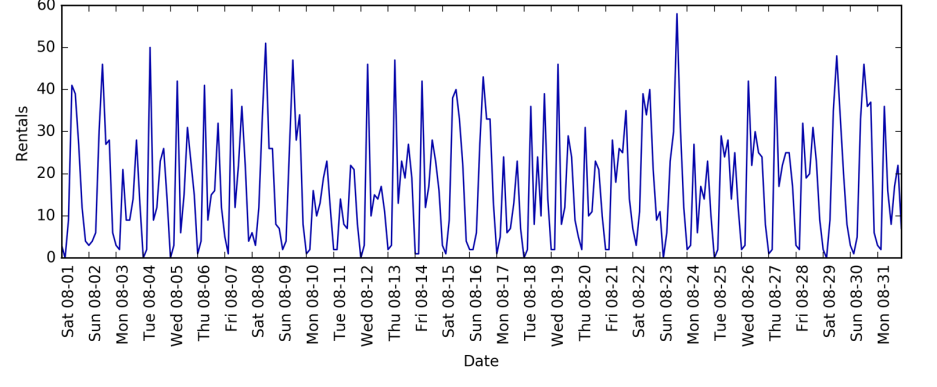
\includegraphics[scale=0.55]{Imagen_Machine/Bike1}
    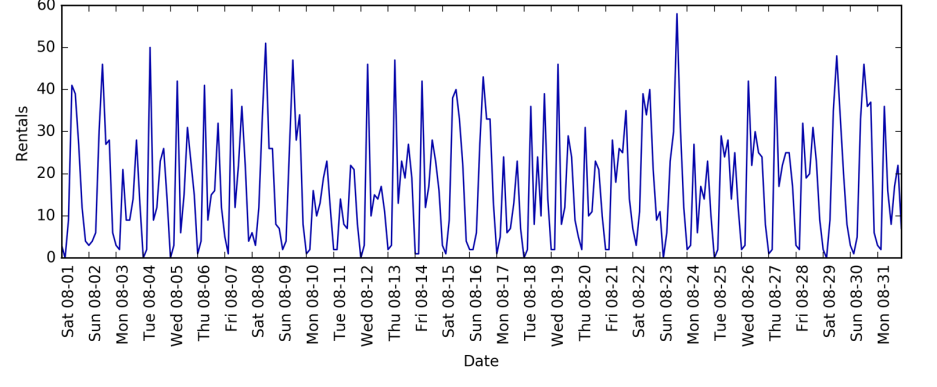
\includegraphics[scale=0.55]{Imagen_Machine/Bike1.png}
	\caption{Número de alquiler de bicicletas en el tiempo para una estación de Citi Bike seleccionada}
	\label{Bike1}
\end{figure}

Si observamos la data, podemos distinguir claramente día y noche para cada ínterval de 24 horas. Los patrones para los días de semana y los fines de semana también parecen ser muy diferentes.  Al evaluar una tarea de predicción en una serie temporal como esta, por lo general queremos aprender del pasado y predecir para el futuro.   Esto significa que al hacer una división en el conjunto de entrenamiento y de pruebas, queremos utilizar todos los datos hasta una fecha determinada como el conjunto de entrenamiento y todos los datos anteriores a esa fecha como el conjunto de pruebas.   
Así es como usualmente usamos la predicción de series de tiempo: dado todo lo que sabemos sobre alquileres en el pasado, ¿Qué crees que sucederá mañana? Utilizaremos los primeros 184 puntos de datos, correspondientes a los primeros 23 días, como el conjunto de entrenamiento, y los 64 puntos de datos restantes, correspondientes a los 8 días restantes, como el conjunto de pruebas.
 
La única característica que estamos utilizando en la tarea de predicción es la fecha y la hora en que se produjo un número particular de alquileres. Por lo tanto, la característica  de entrada es la fecha y hora, digamos, 2015-08-01 00:00:00- y la salida es el número de alquileres en las siguientes tres horas (tres en este caso, de acuerdo con  la {\ttfamily DataFrame}).

Una  manera común de que las fechas se almacenan en las computadoras está utilizando el tiempo POSIX, el cual  es el número de segundos desde enero de 1970 00:00:00 (también conocido como el comienzo del tiempo Unix). Como un primer intento, podemos utilizar esta única característica de entero único como la representación de la data:\\

\begin{lstlisting}%[frame=single]

In[52]:

   # extract the target values (number of rentals)
   y = citibike.values
   # convert the time to POSIX time using "%s"
   X = citibike.index.astype("int64").values.reshape(-1, 1) // 10**9
   # Genera error 
   # X = citibike.index.strftime("%s").astype("int").reshape(-1, 1)
   # por  version anterior
     
\end{lstlisting}

Primero definimos una función para dividir en el conjuntos de entrenamiento y prueba, construir el modelo,
y visualiza el resultado: 

\begin{lstlisting}

In[54]:

   # use the first 184 data points for training, and the rest for testing
   n_train = 184
   
   # function to evaluate and plot a regressor on a given feature set
   def eval_on_features(features, target, regressor):
       # split the given features into a training and a test set
       X_train, X_test = features[:n_train], features[n_train:]
       # also split the target array
       y_train, y_test = target[:n_train], target[n_train:]
       regressor.fit(X_train, y_train)
       print("Test-set R^2: {:.2f}".format(regressor.score(X_test, y_test)))
       y_pred = regressor.predict(X_test)
       y_pred_train = regressor.predict(X_train)
       plt.figure(figsize=(10, 3))
       
       plt.xticks(range(0, len(X), 8), xticks.strftime("%a %m-%d"), 
                  rotation=90, ha="left")
                  
       plt.plot(range(n_train), y_train, label="train")
       plt.plot(range(n_train, len(y_test) + n_train), y_test, '-',
                 label="test")
       plt.plot(range(n_train), y_pred_train, '--', 
                label="prediction train")
       
       plt.plot(range(n_train, len(y_test) + n_train), y_pred, '--',
                label="prediction test")
       plt.legend(loc=(1.01, 0))
       plt.xlabel("Date")
       plt.ylabel("Rentals")

\end{lstlisting}

Como vimos antes,  los bosques aleatorios requieren muy poco preprocesamiento en los datos, lo que hace que 
este parezca un buen modelo para empezar. Usamos la característica X de tiempo POSIX,  y pasamos  a un regresor de bosque aleatorio  la función {\ttfamily  eval\_on\_features}. La Figura \ref{POSIX} muestra el resultado:\\

\begin{lstlisting}%[frame=single]

In[55]:

   from sklearn.ensemble import RandomForestRegressor
   regressor = RandomForestRegressor(n_estimators=100, random_state=0)
   plt.figure()
   eval_on_features(X, y, regressor)

Out[55]:

    Test-set R^2: -0.04

\end{lstlisting}

\begin{figure}[h!]
	\centering
	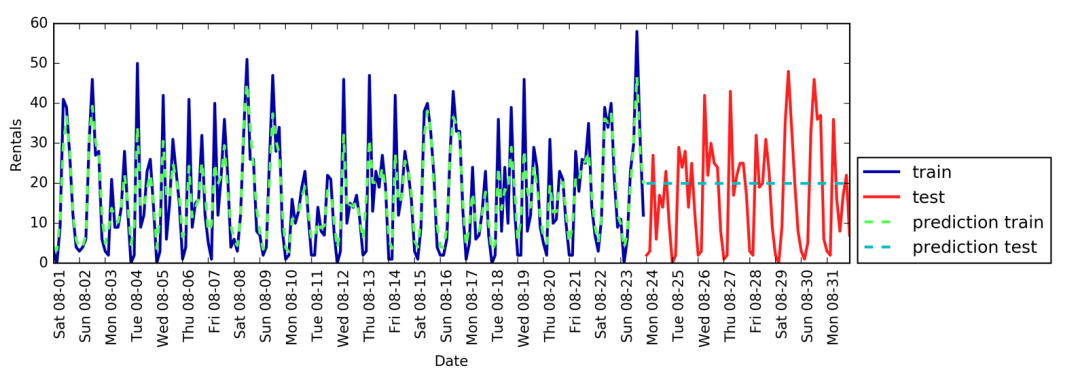
\includegraphics[scale=0.55]{Imagen_Machine/POSIX}
	\caption{Predicciones hechas por un bosque aleatorio usando sólo el tiempo POSIX}
	\label{POSIX}
\end{figure}

Las predicciones sobre el conjunto de entrenamiento son muy buenas, como es habitual para los bosques aleatorios; sin embargo, para el conjunto de pruebas, se predice una línea constante. El $R^{2}$ es -0.03, lo que significa que no aprendimos nada. ¿Qué pasó? \\

El problema radica en la combinación de la característica y el bosque aleatorio. 
El valor de la característica  de tiempo POSIX para el conjunto de prueba está fuera del rango de los valores de la característica en el conjunto de entrenamiento: los puntos en el conjunto de prueba tienen marcas de tiempo que son posteriores a todos los puntos en el conjunto de entrenamiento. 

Los árboles, y por lo tanto los bosques aleatorios, no pueden extrapolarse a rangos fuera del conjunto de entrenamiento. El resultado es que el modelo simplemente predice el valor objetivo del punto más cercano en el conjunto de entrenamiento, que es la última vez que observó cualquier dato.   Claramente podemos hacer algo mejor que esto. Aquí es donde entra nuestro "{}conocimiento experto". Al observar las cifras de alquiler en la data de entrenamiento, dos factores parecen ser muy importantes: la hora del día y el día de la semana.

 Por lo tanto, vamos a añadir estas dos características. Realmente no podemos aprender nada de la hora POSIX, por lo que sacamos esa característica. Primero, usemos sólo la hora del día. Como muestra la Figura \ref{DiaHora}, ahora las predicciones tienen el mismo patrón para cada día de la semana:

\begin{lstlisting}%[frame=single]

In[56]:

   X_hour = citibike.index.hour.values.reshape(-1, 1) 
   #  Error version  X_hour = citibike.index.hour.reshape(-1, 1)
   eval_on_features(X_hour, y, regressor)

Out[56]:

    Test-set R^2: 0.60
 
\end{lstlisting}


\begin{figure}[h!]
	\centering
	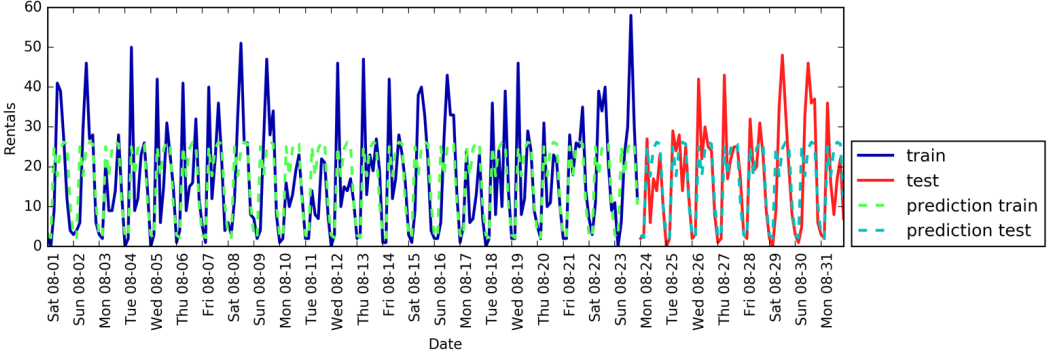
\includegraphics[scale=0.55]{Imagen_Machine/DiaHora}
	\caption{Predicciones hechas por un bosque al azar usando sólo la hora del día}
	\label{DiaHora}
\end{figure}


El $R^{2}$  mejoro  mucho, pero las predicciones claramente  pierden el patrón semanal. Ahora vamos a añadir también el día de la semana (ver Figura \ref{DiaHora2}):

\begin{lstlisting}%[frame=single]

In[57]:

    X_hour_week = np.hstack([citibike.index.dayofweek.values.reshape(-1, 1),
                             citibike.index.hour.values.reshape(-1, 1)])
    #  error 
    # X_hour_week = np.hstack([citibike.index.dayofweek.reshape(-1, 1),
    #                        citibike.index.hour.reshape(-1, 1)])
    eval_on_features(X_hour_week, y, regressor)

Out[57]:

    Test-set R^2: 0.84

\end{lstlisting}


\begin{figure}[h!]
	\centering
	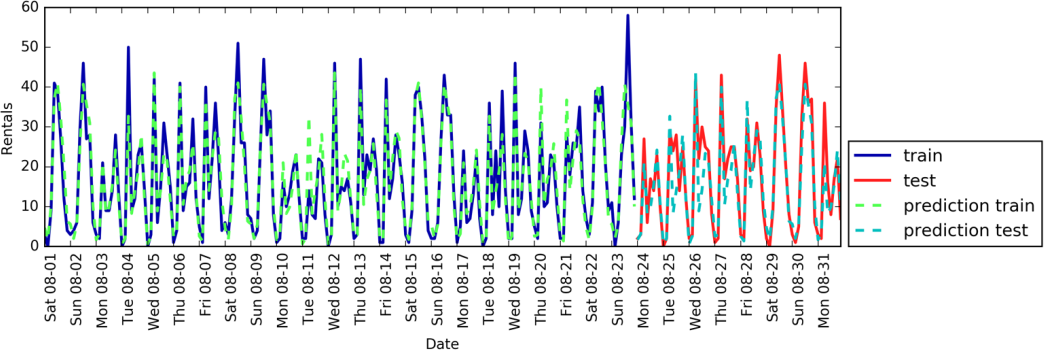
\includegraphics[scale=0.55]{Imagen_Machine/DiaHora2}
	\caption{Predicciones con un bosque aleatorio utilizando las características día de la semana y hora}
	\label{DiaHora2}
\end{figure}


Ahora tenemos un modelo que captura el comportamiento periódico considerando el día de la semana y la hora del día. Tiene un $R^{2}$ de 0.84, y muestra un rendimiento predictivo bastante bueno. 

Lo que este modelo probablemente está aprendiendo es el número promedio de alquileres para cada combinación de día laborable y hora del día a partir de los primeros 23 días de Agosto. Esto en realidad no requiere un modelo complejo como un bosque aleatorio, así que vamos a tratar con un modelo más simple, { \ttfamily  LinearRegression } (ver Figura \ref{DiaHora3}):\\

\begin{lstlisting}%[frame=single]

In[58]:
   
   from sklearn.linear_model import LinearRegression
   eval_on_features(X_hour_week, y, LinearRegression())

Out[58]:

    Test-set R^2: 0.13

\end{lstlisting}



\begin{figure}[h!]
	\centering
	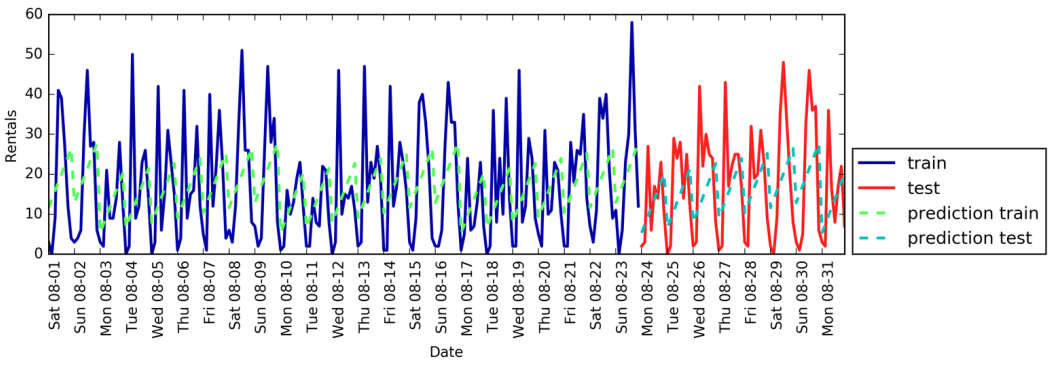
\includegraphics[scale=0.55]{Imagen_Machine/DiaHora3}
	\caption{Predicciones hechas por regresión lineal usando día de semana y hora del día como características}
	\label{DiaHora3}
\end{figure}


El modelo  {\ttfamily LinearRegression}  funciona muy mal o peor, y el patrón periódico parece extraño. 

La razón  para esto es que codificamos día de semana y hora del día usando enteros, el cual es interpretada como variables continuas.  Por lo tanto, el modelo lineal sólo puede aprender una función lineal de la hora del día, y aprendió que más tarde en el día, hay más alquileres. Sin embargo, los patrones son mucho más complejos que eso. Podemos capturar esto interpretando los enteros como variables categóricas, transformándolos usando {\ttfamily One HotEncoder} (ver Figura {DiaHora4}):



\begin{lstlisting}

In[59]:

   enc = OneHotEncoder()
   X_hour_week_onehot = enc.fit_transform(X_hour_week).toarray()
   eval_on_features(X_hour_week_onehot, y, Ridge())

Out[60]:

   Test-set R^2: 0.62

\end{lstlisting}


\begin{figure}[h!]
	\centering
	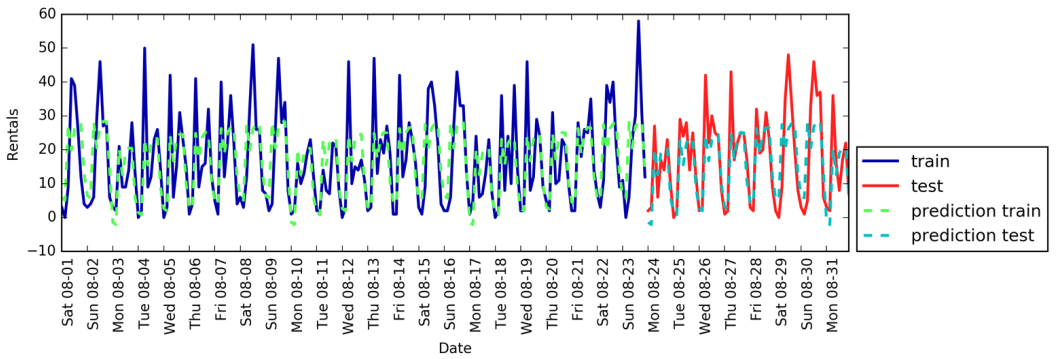
\includegraphics[scale=0.55]{Imagen_Machine/DiaHora4}
	\caption{Predicciones hechas por regresión lineal usando la codificación one-hot del día y del día de la semana}
	\label{DiaHora4}
\end{figure}

Esto nos da un mejor resultado  que la codificación de características como continua. Ahora el modelo lineal aprende un coeficiente para cada día de la semana, y un coeficiente para cada hora del día. Eso significa que el patrón de "{}hora del día"{} se comparte durante todos los días de la semana.\\

% un sin embargo...

Usando  interacción de características, podemos permitir que el modelo aprenda un coeficiente para cada combinación de día y hora del día (ver Figura \ref{DiaHora5}):



\begin{lstlisting}%[frame=single]

In[61]:

   poly_transformer = PolynomialFeatures(degree=2, interaction_only=True,
                                         include_bias=False)
   X_hour_week_onehot_poly = poly_transformer.fit_transform(X_hour_week_onehot)
   lr = Ridge()
   eval_on_features(X_hour_week_onehot_poly, y, lr)

Out[61]:

   Test-set R^2: 0.85

\end{lstlisting}



\begin{figure}[h!]
	\centering
	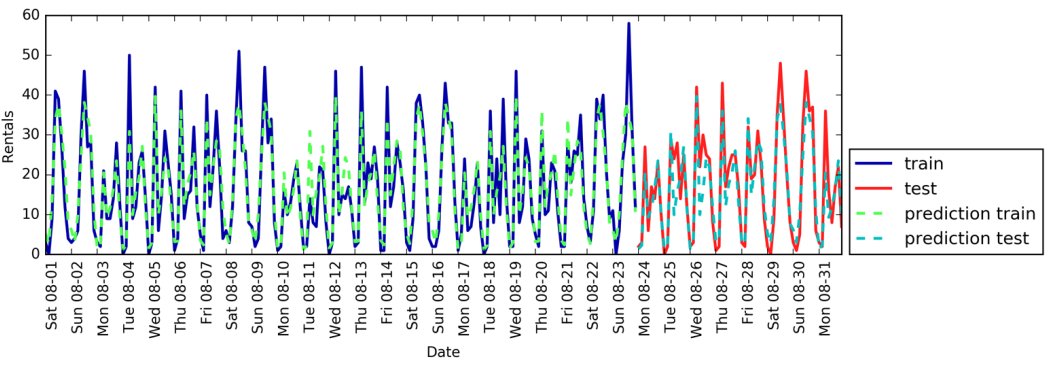
\includegraphics[scale=0.55]{Imagen_Machine/DiaHora5}
	\caption{Predicciones hechas por regresión lineal usando un producto  de las características   día de la semana y  hora del día}
	\label{DiaHora5}
\end{figure}

Esta transformación finalmente produce un modelo que funciona de manera similarmente bien  al  bosque aleatorio. Un gran beneficio de este modelo es que está muy claro lo que es aprendido: un coeficiente para cada día y hora. Podemos simplemente gráficar  los coeficientes aprendidos por el modelo, algo que no sería posible para el bosque aleatorio.\\

  Primero, creamos nombres de características para la hora y día:




\begin{lstlisting}%[frame=single]

In[62]:

   hour = ["%02d:00" % i for i in range(0, 24, 3)]
   day = ["Mon", "Tue", "Wed", "Thu", "Fri", "Sat", "Sun"]
   features = day + hour

\end{lstlisting}


Luego nombramos todas las características de interacción extraídas por {\ttfamily PolynomialFeatures}, usando el método {\ttfamily get\_feature\_names}, y mantenemos sólo las características con coeficientes distinto de cero:\\



\begin{lstlisting}%[frame=single]

In[63]:

   features_poly = poly_transformer.get_feature_names(features)
   features_nonzero = np.array(features_poly)[lr.coef_ != 0]
   coef_nonzero = lr.coef_[lr.coef_ != 0]

\end{lstlisting}



Ahora podemos visualizar los coeficientes aprendidos por el modelo lineal, como se ve en la Figura \ref{ProducHora}:\\

\begin{lstlisting}%[frame=single]

In[64]:

   plt.figure(figsize=(15, 2))
   plt.plot(coef_nonzero, 'o')
   plt.xticks(np.arange(len(coef_nonzero)), features_nonzero, rotation=90)
   plt.xlabel("Feature magnitude")
   plt.ylabel("Feature")

\end{lstlisting}



\begin{figure}[h!]
	\centering
	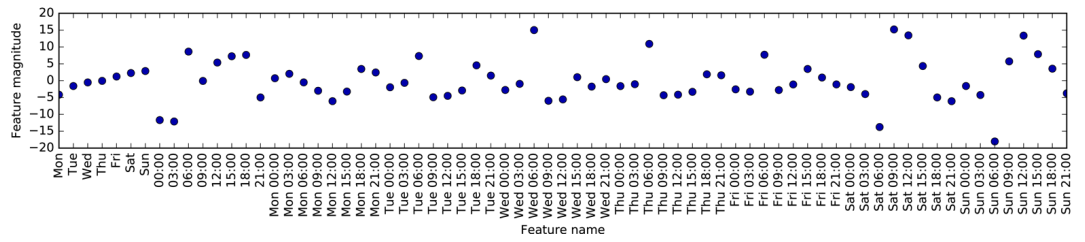
\includegraphics[scale=0.55]{Imagen_Machine/ProducHora}
	\caption{Coeficientes del modelo de regresión lineal utilizando un producto de hora y día}
	\label{ProducHora}
\end{figure}



\section{Resumen y perspectivas}

%  suitable  =   adecuado 

En este capítulo, discutimos cómo tratar los diferentes tipos de datos (en particular, con variables categóricas). Enfatizamos la importancia de representar los datos de una manera que sea adecuada para el algoritmo de aprendizaje automático, por ejemplo, mediante la codificación {\ttfamily one-hot-encoding}.


También discutimos la importancia de la ingeniería de nuevas características, y la posibilidad de utilizar el conocimiento experto en la creación de características derivadas de sus datos. 

En particular, los modelos lineales podrían beneficiarse en gran medida de la generación de nuevas características a través de {\ttfamily binning} y la adición de polinomios e interacciones,mientras que los modelos no lineales más complejos como los bosques aleatorios y las SVMs podrían ser capaces de aprender tareas más complejas sin expandir explícitamente el espacio de características.
En la práctica, las características que se utilizan (y la coincidencia entre las características y el método) es a menudo la pieza más importante para hacer que un enfoque de aprendizaje automático funcione bien.
 

Ahora que usted tiene una buena idea de cómo representar los datos de una manera apropiada y qué algoritmo utilizar para la tarea, el próximo capítulo se centrará en la evaluación del rendimiento de los modelos de aprendizaje automático y la selección de la configuración de parámetros adecuados.

%%%%%%%%%%%                 %%%%%%%%%%%%%%%%%%%%%%%%%%
   

	
	\chapter{Evaluación y selección de  parámetros  para  mejorar el modelo}{\label{Cap5}}
                   %	selección de los parámetros

Habiendo discutido los fundamentos del aprendizaje supervisado y no supervisado, y
explorado una variedad de algoritmos de aprendizaje automático, ahora iremos un poco  más
profundo en la evaluación del modelos y selección de los parámetros.\\

Nos centraremos en los métodos supervisados, la regresión y la clasificación, ya que   evaluar 
y  seleccionar modelos del aprendizaje no supervisado es a generalmente  un proceso muy cualitativo (como
vimos en el Capítulo \ref{Cap3}).\\


Para evaluar los modelos supervisados, hasta ahora hemos dividido la data dos conjuntos, uno de  entrenemiento  y el otro  de prueba con la función {\ttfamily train\_test\_split}, y se  construye  un modelo sobre el conjunto de  entrenamiento con el método de ajuste y se evaluá en el conjunto de prueba usando el método de puntuación (score), el cual para la clasificación calcula la fracción de muestras clasificadas correctamente. A continuación se presenta un ejemplo de ese proceso:


\begin{lstlisting}%[frame=single]

In[2]:

   from sklearn.datasets import make_blobs
   from sklearn.linear_model import LogisticRegression
   from sklearn.model_selection import train_test_split
   
   # create a synthetic dataset
   X, y = make_blobs(random_state=0)
   # split data and labels into a training and a test set
   X_train, X_test, y_train, y_test = train_test_split(X, y, random_state=0)
   # instantiate a model and fit it to the training set
   logreg = LogisticRegression().fit(X_train, y_train)
   # evaluate the model on the test set
   print("Test set score: {:.2f}".format(logreg.score(X_test, y_test)))

Out[2]:

    Test set score: 0.88

\end{lstlisting}


Recuerde que la razón por la que dividimos la data  en los dos conjuntos (entrenamiento y prueba) es por el interés de medir qué tan bien el modelo logra generaliza en una data nueva y nunca antes tratada o vista.  En este caso no nos interesa qué tan bien el modelo se ajusta al conjunto de entrenamiento, sino más bien 
qué tan bien  hace predicciones con datos que no se observaron durante el entrenamiento.\\

En este capítulo, ampliaremos dos aspectos de esta evaluación.  Primero introduciremos la validación cruzada, una forma más robusta de evaluar el rendimiento de la generalización, y se discute métodos para evaluar el rendimiento de clasificación y regresión que van  más allá de las medidas predeterminadas de  exactitud  y $ R^{2} $  proporcionadas por el método de puntuación ({\ttfamily score}).\\

También discutiremos la búsqueda de cuadrícula (grid search), un método efectivo para ajustar los 
parámetros en modelos supervisados para el mejor rendimiento de generalización.




\section{Validación cruzada}

%    En la validación cruzada de K iteraciones o K-fold cross-validatio los datos
%     de muestra se dividen  en   K subconjuntos



La validación cruzada es un método estadístico para evaluar el rendimiento de generalización que
es más estable y completo,  que usar una división en un conjunto de entrenamiento y prueba.  En la validación cruzada, la data es particionada repetidamente y se entrenan varios modelos.   La versión más utilizada de la validación cruzada es la validación cruzada k-fold, conocido como validación cruzada de K iteraciones (K-fold cross-validation\footnote{K-Folds por su traducción al español podríamos interpretarla como K-Dobleces. Esto es porque hacemos k particiones de la data de tamaño N antes de dividirla en p particiones de entrenamiento y prueba.}), en este caso la data de muestra se dividen en K subconjuntos. Uno de los subconjuntos se utiliza como data de prueba y el resto (K-1) como datos de entrenamiento. En parámetro  k es un número especificado por el usuario, generalmente 5 o 10.  Al realizar una validación cruzada de 5-fold, la data es particionada  primero en cinco partes de  igual tamaño (aproximadamente), llamadas folds.
Sequidamente, se entrena una secuencia de modelos. El primer modelo se entrena  utilizando el primer fold  como el conjunto de prueba y los  restantes (2–5) se utilizan como conjunto de entrenamiento. 

El modelo es construido usando la data en los   2–5 folds, y  la exactitud  se evalúa en el 
primer fold. Luego se construye otro modelo, esta vez usando el fold 2 como el conjunto de 
prueba y la data en los folds 1, 3, 4 y 5 como el conjunto de entrenamiento. Este proceso se repite 
usando  fold 3, 4 y 5 como conjuntos de pruebas. Para cada una de estas cinco divisiones
 de los datos en conjuntos de entrenamiento y pruebas, se calcula la exactitud. Al final, hemos 
 calculado cinco valores de exactitud. El  proceso se ilustra en  la  Figura \ref{Validacion1}:


\begin{lstlisting}%[frame=single]

In[3]:

   mglearn.plots.plot_cross_validation()

\end{lstlisting}



\begin{figure}[h!]
	\centering
	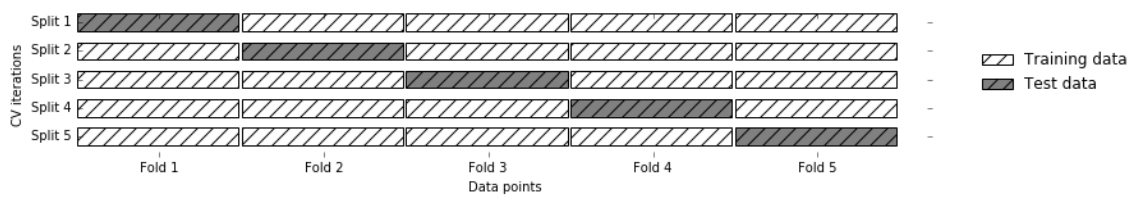
\includegraphics[scale=0.55]{Imagen_Machine/Validacion1}
	\caption{División de la data en validación cruzada con 5-fold}
	\label{Validacion1}
\end{figure}




Por lo general, el primer quinto de los datos es el primer fold, el segundo quinto de los datos es el segundo  fold, y así sucesivamente.


\subsection{Validación cruzada  en scikit-learn}
				% verdad fundamental = ground-truth
				
La validación cruzada se implementa en {\ttfamily  scikit-learn} usando la función {\ttfamily cross\_val\_score} del módulo {\ttfamily  model\_selection}. Los parámetros de la función  {\ttfamily cross\_val\_score}  son el modelo que queremos evaluar, la data de entrenamiento y las etiquetas {\ttfamily ground-truth}.     


Vamos a evaluar  el modelo  {\ttfamily  LogisticRegression} en el conjunto de la data Iris:

\begin{lstlisting}%[frame=single]

In[4]:

   from sklearn.model_selection import cross_val_score
   from sklearn.datasets import load_iris
   from sklearn.linear_model import LogisticRegression
   iris = load_iris()
   logreg = LogisticRegression()
   scores = cross_val_score(logreg, iris.data, iris.target)
   print("Cross-validation scores: {}".format(scores))

Out[4]:
 
    Cross-validation scores: [ 0.961 0.922 0.958]

\end{lstlisting}



Por defecto,  {\ttfamily cross\_val\_score}  realiza tres-fold para la validación cruzada,
 devolviendo tres valores de exactitud. Podemos cambiar el número de  folds 
 cambiando el  parámetro {\ttfamily cv}:


\begin{lstlisting}%[frame=single]

In[5]:

   scores = cross_val_score(logreg, iris.data, iris.target, cv=5)
   print("Cross-validation scores: {}".format(scores))

Out[5]:
    
    Cross-validation scores: [ 1. 0.967 0.933 0.9 1. ]

\end{lstlisting}


Una forma común de resumir la exactitud   de la validación cruzada es calcular la media:

\begin{lstlisting}%[frame=single]

In[6]:

   print("Average cross-validation score: {:.2f}".format(scores.mean()))

Out[6]:

    Average cross-validation score: 0.96

\end{lstlisting}

Usando la media de validación cruzada podemos concluir que en general se espera que el modelo sea alrededor del 96\%  exacto  en promedio. Mirando las cinco puntuaciones producidas por la validación cruzada de 5-folds, también podemos concluir que hay una varianza relativamente alta en la exactitud entre los  folds, que van de 100\%   hasta 90\%  de  exactitud. 

Esto podría implicar que el modelo es muy dependiente de los folds  particulares utilizados para el entrenamiento, pero también podría ser sólo una consecuencia del tamaño del conjunto de datos, que en este caso es muy pequeño.


\subsubsection{Beneficios de la validación cruzada}

Hay varios beneficios al usar la validación cruzada en lugar de una sóla división para la data (en dos conjuntos, el de entrenamiento y el de prueba). Primero, recuerde que {\ttfamily train\_test\_split} realiza 
{\bf{división aleatoria}} de la data.  Imagine que somos "{}afortunados"{} al dividir aleatoriamente los datos, y
todos los ejemplos que son difíciles de clasificar terminan en el conjunto de entrenamiento.
En ese caso, el conjunto  de  prueba  solo contendrá ejemplos "{}fáciles"{}, y 
la  exactitud en el conjunto de prueba será alta, un poco real. Por el contrario, si somos "{}desafortunados"{}, podríamos haber obtenido  aleatoriamente todos los ejemplos difíciles de clasificar en el conjunto de prueba y, en consecuencia, se obtendrá un puntaje de exactitud es bajo, nuevamente poco real. Sin embargo, cuando se utiliza la validación cruzada, cada dato estará en el conjunto de entrenamiento exactamente una vez:  cada dato está en uno de los  folds, y cada  fold es el conjunto de prueba una vez. 


Por lo tanto, el modelo necesita generalizar bien a todas las muestras en el conjunto de datos para que todas las puntuaciones de validación cruzada (y su media) sean altas.  Teniendo  múltiples divisiones de los datos también proporciona información sobre lo sensible que es el modelo a la selección del conjunto de datos de entrenamiento.  Para la data Iris, vimos exactitudes entre 90\% y 100\%.  Este es un rango bastante amplio y nos proporciona una idea sobre cómo podría funcionar el modelo en el peor de los casos y en los mejores escenarios cuando se aplica a nuevos datos.

Otro beneficio de la validación cruzada en comparación con el uso de una sóla división de los datos, es
que usamos nuestros datos de manera más efectiva. Cuando usamos  {\ttfamily train\_test\_split}, usualmente usamos 75\% de los datos para el entrenamiento  y 25\% de los datos para evaluación. Cuando se usan 5-folds en  validación cruzada, en cada iteración podemos usar cuatro quintos de los datos (80\%) para ajustar el
modelo.  Cuando usamos la validación cruzada con 10-folds, podemos usar nueve décimas de los datos
(90\%) para ajustar al modelo. Con más datos generalmente dará como resultado modelos más precisos.


La principal desventaja de la validación cruzada es el aumento del costo computacional. Como estamos 
ahora entrenando k modelos en lugar de un sólo modelo, la validación cruzada será aproximadamente k
veces más lento en comparación con una sóla división de los datos.\\
% Zorrillo


\begin{minipage}[t]{0.2\textwidth}
	\centering\raisebox{\dimexpr \topskip-\height}{%
		
\includegraphics[width=\textwidth]{Imagen_Machine/Zorrillo}}
\end{minipage}%\hfill
\begin{minipage}[t]{0.75\textwidth} 
	{\scriptsize		
		Es importante tener en cuenta que la validación cruzada no es una forma de
		construir un modelo que se pueda aplicar a nuevos datos. Validación cruzada
		"{}No"{} devuelve un modelo. 		
		Al aplicar {\ttfamily cross\_val\_score}, múltiples los modelos se construyen internamente, pero el propósito de la validación cruzada es sólo para evaluar qué tan bien se generalizará un algoritmo dado, cuando es entrenado en un conjunto de datos específico.}
\end{minipage}\\




\subsection{Validación cruzada K-Fold estratificada y otras estrategias}

Dividir el conjunto de datos en k-folds  comenzando con la k-ésima   primera parte de los datos, 
descrito como en la sección anterior, puede que no siempre sea una buena idea. Por ejemplo, vamos
echar un vistazo a la data Iris:

% {\ttfamily cross\_val\_score} 


\begin{lstlisting}%[frame=single]

In[7]:

   from sklearn.datasets import load_iris
   iris = load_iris()
   print("Iris labels:\n{}".format(iris.target))

Out[7]:

    Iris labels:
    [0 0 0 0 0 0 0 0 0 0 0 0 0 0 0 0 0 0 0 0 0 0 0 0 0 0 0 0 0 0 0 0 0 0 0 0 0
     0 0 0 0 0 0 0 0 0 0 0 0 0 1 1 1 1 1 1 1 1 1 1 1 1 1 1 1 1 1 1 1 1 1 1 1 1
     1 1 1 1 1 1 1 1 1 1 1 1 1 1 1 1 1 1 1 1 1 1 1 1 1 1 2 2 2 2 2 2 2 2 2 2 2
     2 2 2 2 2 2 2 2 2 2 2 2 2 2 2 2 2 2 2 2 2 2 2 2 2 2 2 2 2 2 2 2 2 2 2 2 2
     2 2]

\end{lstlisting}


Como puede ver, el primer tercio de los datos es la clase 0, el segundo tercio es la clase 1,
y el último tercio es la clase 2. Imagine hacer una validación cruzada con 3-fold  en esta data.
El primer fold sería sólo de clase 0, por lo que en la primera división de los datos, el conjunto de prueba sería sólo clase 0, y el conjunto de entrenamiento sería sólo clases 1 y 2.   Como las clases de entrenamiento y pruebas serían diferentes en las tres divisiones, las tres
medidas de exactitud  de la validación cruzada sería cero en este conjunto de datos. Eso no es muy útil, cómo  podemos obtener una mejor  de exactitud en la data Iris. 

Como la simple estrategia de k-fold falla aquí, {\ttfamily scikit-learn}  no la usa para clasificación, sino que utiliza estratificación de k -fold para la validación cruzada.
La validación cruzada estratificada,  dividen los datos de manera que las proporciones entre clases sean las mismas en cada fold, de acuerdo como están distribuidas en todo el conjunto de datos, en la  Figura \ref{Validacion2}  se ilustra la idea: 

\begin{lstlisting}%[frame=single]

In[8]

   mglearn.plots.plot_stratified_cross_validation()
   
\end{lstlisting}

\begin{figure}[h!]
	\centering
	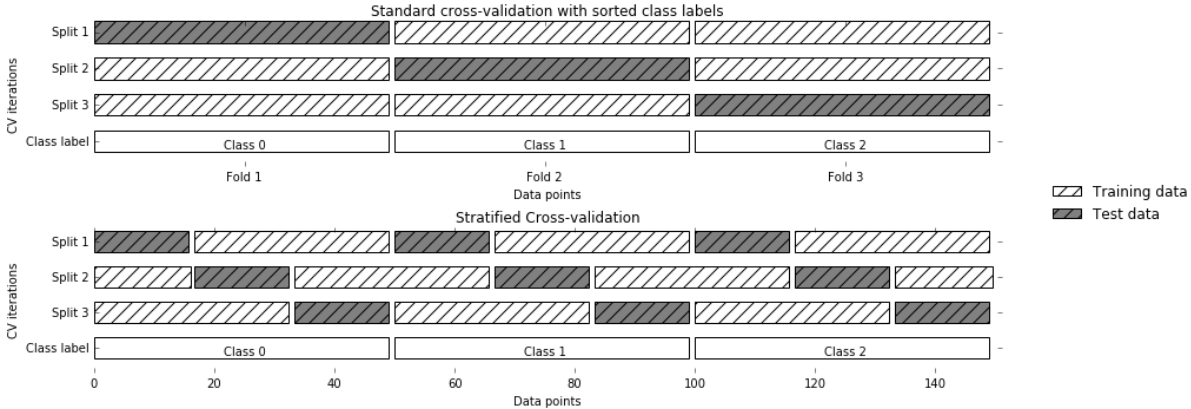
\includegraphics[scale=0.53]{Imagen_Machine/Validacion2}
	\caption{Comparación de validación cruzada estándar y validación cruzada estratificada
		cuando los datos se ordenan por etiqueta de clase}
	\label{Validacion2}
\end{figure}


Por ejemplo, si el 90\% de las  muestras pertenecen a la clase A y el 10\%  a 
pertenecen a la clase B, entoces  la validación cruzada estratificada asegura que en cada fold, haya el 90\% de las muestras pertenecen a la clase A y el 10\% de las muestras pertenecen a la clase B.

Por lo general, es una buena idea utilizar la validación cruzada de k-fold estratificada en lugar de k-fold
validación cruzada para evaluar un clasificador, porque produce resultados de estimaciones más confiables del rendimiento de generalización. 

En el caso de solo el 10\% de las muestras pertenecientes a la clase B, usando la validación cruzada estándar de k-fold, puede suceder fácilmente que sólo una contenga las  muestras de la clase A. 
El uso de este fold  como conjunto de prueba no sería muy informativo sobre el rendimiento general del clasificador.\\


Para la regresión, {\ttfamily scikit-learn} utiliza la validación cruzada k-fold estándar (standard k-fold cross-validation) de forma predeterminada. Eso sería posible también  tratar  de hacer que cada fold  sea representativo de los diferentes valores  que tiene el objetivo de regresión, pero esto no es una estrategia comúnmente utilizada y sería sorprendente para la mayoría de los usuarios.

\subsubsection{Más control sobre la validación cruzada}\label{VC}


Vimos anteriormente que podemos ajustar el número de folds que se usa  en {\ttfamily cross\_val\_score} mediante  el parámetro {\ttfamily cv}.   Sin embargo, {\ttfamily scikit-learn} permite un control mucho más fino sobre lo que sucede durante la división de la data al proporcionar un divisor de validación cruzada como el parámetro {\ttfamily cv}.  Para la mayoría de los casos de uso, los valores por defecto de la validación cruzada de k-fold para regresión y la  estratificado k-fold para clasificación funcionan bien, pero hay algunos casos en los que es posible que podria querer  utilizar una estrategia diferente; digamos, por ejemplo, que queremos usar la validación cruzada estándar k-fold en un conjunto 
de datos de clasificación para reproducir los resultados de otra persona.  Para esto, primero tenemos 
que importar la clase divisor de {\ttfamily KFold} desde el módulo {\ttfamily model\_selection} e instanciarla con el número de fold que  queremos usar:

\begin{lstlisting}%[frame=single]

In[9]:

   from sklearn.model_selection import KFold
   kfold = KFold(n_splits=5)

\end{lstlisting}


Entonces,  podemos pasar el objeto divisor {\ttfamily kfold} como el parámetro {\ttfamily cv} a {\ttfamily cross\_val\_score}:

\begin{lstlisting}%[frame=single]

In[10]:
  
   print("Cross-validation scores:\n{}".format(
          cross_val_score(logreg, iris.data, iris.target, cv=kfold)))

Out[10]:
    
    Cross-validation scores:
    [ 1. 0.933 0.433 0.967 0.433]

\end{lstlisting}

De esta forma, podemos verificar que es realmente una mala idea usar tres-fold (no estratificado) para la  validación cruzada en la data Iris:

\begin{lstlisting}%[frame=single]

In[11]:

   kfold = KFold(n_splits=3)
   print("Cross-validation scores:\n{}".format(
          cross_val_score(logreg, iris.data, iris.target, cv=kfold)))

Out[11]:

    Cross-validation scores:
    [ 0. 0. 0.]

\end{lstlisting}


Recuerde: cada  fold   corresponde a una de las clases del conjunto de data Iris, por lo que no se puede aprender nada. Otra forma de resolver este problema es barajando (aleatorio) los datos, en lugar de estratificar los folds, para eliminar o remover el orden de las muestras por etiqueta. Podemos hacerlo configurando el parámetro {\ttfamily shuffle} de {\ttfamily  KFold} como {\ttfamily True}. Si barajamos los datos, también necesitamos arreglar el estado aleatorio {\ttfamily random\_state} para obtener un barajamiento reproducible. De lo contrario, cada ejecución de {\ttfamily cross\_val\_score} daría un resultado diferente, ya que cada vez que  se use generá una división diferente (esto podría no ser un problema, pero puede  sorprender). Barajando los datos antes de dividirlos se obtiene un resultado mucho mejor:

\begin{lstlisting}%[frame=single]

In[12]:
   
   kfold = KFold(n_splits=3, shuffle=True, random_state=0)
   print("Cross-validation scores:\n{}".format(
          cross_val_score(logreg, iris.data, iris.target, cv=kfold)))
   
Out[12]:

    Cross-validation scores:
    [ 0.9 0.96 0.96]
    
\end{lstlisting}


\subsubsection{Validación cruzada de dejando uno fuera	\\ Leave-one-out} 


Otro método de validación cruzada frecuentemente usado es {\emph{dejar-uno-fuera (leave-one-out)}}, implementado en {\ttfamily LeaveOneOut}. Puedes pensar en la validación cruzada dejar-uno-fuera,  como una validación cruzada de k-fold donde cada fold  es una sóla muestra. Para cada división,  elige un sólo punto de la data para ser el conjunto de prueba. Esto puede llevar mucho tiempo, especialmente para grandes conjuntos de datos, pero a veces proporciona mejores estimaciomes en conjuntos pequeños:


\begin{lstlisting}%[frame=single]

In[13]:

   from sklearn.model_selection import LeaveOneOut
   loo = LeaveOneOut()
   scores = cross_val_score(logreg, iris.data, iris.target, cv=loo)
   print("Number of cv iterations: ", len(scores))
   print("Mean accuracy: {:.2f}".format(scores.mean()))

Out[13]:

    Number of cv iterations: 150
    Mean accuracy: 0.95

\end{lstlisting}



En la  validación cruzada dejando uno fuera o Leave-one-out cross-validation (Loovc) implica separar los datos de forma que para cada iteración tengamos una sola muestra para los datos de prueba y todo el resto conformando los datos de entrenamiento. La evaluación viene dada por el error, y en este tipo de validación cruzada el error es muy bajo, pero en cambio, a nivel computacional es muy costoso, puesto que se tienen que realizar un elevado número de iteraciones, tantas como N muestras tengamos y para cada una analizar los datos tanto de entrenamiento como de prueba.




\subsubsection{Validación cruzada Shuffle-split} 

%     Shuffle-split cross-validation



Otra estrategia muy flexible para la validación cruzada es la validación cruzada de  {\ttfamily shuffle-split}.  En la validación cruzada {\ttfamily shuffle-split}, cada muestra dividida tiene muchos puntos tanto para el conjunto de entrenamiento  {\ttfamily  train\_size} como para conjunto de prueba {\ttfamily test\_size} (disjuntos). Esta división es repetida {\ttfamily  n\_iter} veces. La Figura \ref{Barajar} ilustra una ejecución con cuatro iteraciones para dividir una data que consta de 10 puntos, en  el conjunto de entrenamiento con 5 puntos y el de pruebas con  2 puntos (puede usar enteros para {\ttfamily  train\_size}  y {\ttfamily test\_size} para usar tamaños absolutos para estos conjuntos, o números de punto flotante  (floating-point)  para usar fracciones de todo el conjunto de datos).


\begin{lstlisting}%[frame=single]

In[14]:

   mglearn.plots.plot_shuffle_split()

\end{lstlisting}


\begin{figure}[h!]
	\centering
	%\includegraphics[scale=0.55]{../Imagen_Machine/Barajar}
	\includegraphics[scale=0.55]{Imagen_Machine/Barajar.png}
	\caption{ {\ttfamily ShuffleSplit} con 10 puntos, {\ttfamily train\_size=5,  test\_size=2},  y  {\ttfamily  n\_iter=4}}
	\label{Barajar}
\end{figure}



El siguiente código divide el conjunto de datos en un 50\% para la data de entrenamiento y 
 50\% para el de pruebas con 10 iteraciones:


\begin{lstlisting}%[frame=single]

In[15]:

   from sklearn.model_selection import ShuffleSplit
   shuffle_split = ShuffleSplit(test_size=.5, train_size=.5, n_splits=10)
   scores = cross_val_score(logreg, iris.data, iris.target, cv=shuffle_split)
   print("Cross-validation scores:\n{}".format(scores))
   
Out[15]:

   Cross-validation scores:
   [ 0.96 0.907 0.947 0.96 0.96 0.907 0.893 0.907 0.92 0.973]
  
\end{lstlisting}

La validación cruzada de Shuffle-split permite controlar el número de iteraciones independientemente de los tamaños de entrenamiento y prueba, lo que a veces puede ser útil. También permite usar sólo una parte de los datos en cada iteración, proporcionando configuraciones para {\ttfamily train\_size}  y  {\ttfamily test\_size} que no suman uno.  Submuestreando la data de esta manera, puede ser útil para experimentar con grandes conjuntos de datos.\\

 También hay una variante estratificada de {\ttfamily  ShuffleSplit}, acertadamente llamada {\ttfamily  StratifiedShuffleSplit}, que puede proporcionar resultados más fiables para las tareas de clasificación.



\subsubsection{Validación cruzada con grupos}



Otra configuración muy común para la validación cruzada es cuando hay grupos en la
data que están altamente relacionados. Digamos que quieres construir un sistema para reconocer emociones
a partir de imágenes de caras, y usted recopila un conjunto de datos de imágenes de 100 personas, donde cada
la persona es capturada varias veces, mostrando varias emociones. El objetivo es construir un
clasificador que pueda identificar correctamente las emociones de las personas que no están en el conjunto de datos.  Podrías usar la validación cruzada estratificada por defecto para medir el rendimiento de un clasificador. Sin embargo, es probable que las imágenes de la misma persona estén en ambos conjuntos, en el de entrenamiento y en el de prueba. Será mucho más fácil para un clasificador detectar emociones en una cara que es parte del conjunto de entrenamiento, en comparación con una cara completamente nueva.   Por lo tanto,  para evaluar la exactitud de generalización a nuevas caras,  debemos asegurarnos  que  los conjuntos de  entrenamiento y de prueba contienen imágenes de diferentes personas.\\

 
Para lograr esto, podemos usar {\ttfamily GroupKFold}, que toma un arreglo de grupos como argumento, que podemos usar para indicar qué persona está en la imagen. Los arrreglos de grupos aquí indican  grupos en la data  que no deben dividirse al crear los conjuntos de entrenamiento y prueba, y no debe confundirse con la etiqueta de clase. \\



 Este ejemplo de grupos en los datos es común en aplicaciones médicas, donde
pueden tener múltiples muestras del mismo paciente, pero están interesadas en generalizar
a nuevos pacientes. Del mismo modo, en el reconocimiento de voz, puede tener múltiples grabaciones
de la  misma persona en la data, pero el interés está centrado  en reconocer la voz de nuevas personas.\\


El siguiente es un ejemplo del uso de un conjunto de datos sintético con una agrupación dada por
un arreglo de grupos. La data  consta de 12 puntos,  para cada uno de los puntos, 
el grupos especifica a qué grupo (piensa en pacientes) pertenece el punto. Los grupos especifican
que hay cuatro grupos, y las primeras tres muestras pertenecen al primer grupo, las siguientes cuatro muestras pertenecen al segundo grupo, y así sucesivamente:

\begin{lstlisting}%[frame=single]

In[17]:

   from sklearn.model_selection import GroupKFold
   # create synthetic dataset
   X, y = make_blobs(n_samples=12, random_state=0)
   # assume the first three samples belong to the same group,
   # then the next four, etc.
   groups = [0, 0, 0, 1, 1, 1, 1, 2, 2, 3, 3, 3]
   scores = cross_val_score(logreg, X, y, groups, cv=GroupKFold(n_splits=3))
   print("Cross-validation scores:\n{}".format(scores))

Out[17]:

    Cross-validation scores:
    [ 0.75 0.8 0.667]

\end{lstlisting}


Las muestras no necesitan ser ordenadas por grupo; simplemente hicimos esto con propósito de ilustrar. Las divisiones son calculadas en base a estas etiquetas que se visualizan en la Figura \ref{GrupoArray}.

\begin{lstlisting}%[frame=single]

In[17]:

mglearn.plots.plot_label_kfold()


\end{lstlisting}%[frame=single]


\begin{figure}[h!]
	\centering
	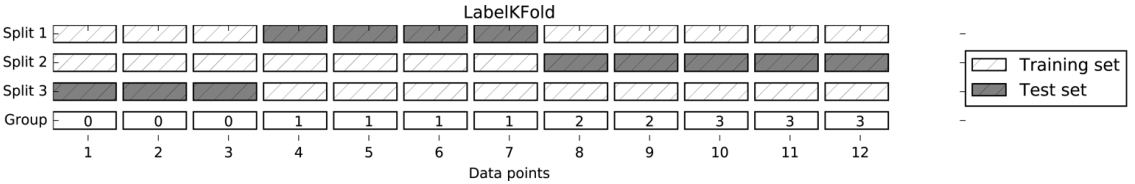
\includegraphics[scale=0.55]{Imagen_Machine/GrupoArray}
	\caption{División dependiente de etiquetas con {\ttfamily GroupKFold}}
	\label{GrupoArray}
\end{figure}

%    Label-dependent splitting with GroupKFold


Como puede ver, por cada división (split $i$), cada grupo está completamente en el conjunto de entrenamiento o completamente en el conjunto de pruebas.


Hay más estrategias de división para la validación cruzada en {\ttfamily scikit-learn}, que permiten una mayor variedad de casos de uso (puede encontrar estos en la guía del usuario de \href{https://scikit-learn.org/stable/modules/cross_validation.html}{\textcolor{red}{\ttfamily scikit-learn}}). Sin embargo, el estándar  {\ttfamily KFold, StratifiedKFold} y  {\ttfamily  GroupKFold } son los más comunmente usados.


\subsubsection{Búsqueda de cuadrícula}

%    Grid Search

Ahora que sabemos cómo evaluar qué tan bien generaliza un modelo, podemos tomar el
siguiente paso y mejorar el rendimiento de generalización del modelo ajustando sus parámetros.  Discutimos la configuración de parámetros de muchos de los algoritmos en 
en los capítulos \ref{Cap2}  y  \ref{Cap3}, y su importancia de entender qué significan los parámetros
antes de intentar ajustarlos. 

 
Encontrar los valores de los parámetros importantes de un  modelo (los que proporcionan el mejor rendimiento de generalización) es una tarea difícil, pero necesario para casi todos los modelos y conjuntos de datos. Debido a que es una tarea tan común,   {\ttfamily scikit-learn} proporciona  métodos estándar  para ayudarte con esto.  El método    más común es la búsqueda de cuadrícula (grid search), que básicamente significa probar todas las combinaciones posibles de parámetros de interés. 


Considere el caso de un kernel SVM con un kernel RBF (función de base radial), como
es implementado en la clase SVC. Como discutimos en el Capítulo \ref{Cap2}, hay dos 
parámetros  importantes: el ancho de banda del kernel, gamma, y el parámetro C  de regularización.  Digamos que desea probar los valores 0.001, 0.01, 0.1, 1, 10 y 100 para el parámetro C, y los mismos valores para gamma.

Ya que tenemos seis configuraciones diferentes para C y gamma  que queremos probar,  tenemos 36 combinaciones de parámetros en total. Observando todas las combinaciones posibles se crea una tabla (o cuadrícula) de configuraciones de parámetros para el SVM, como se muestra aquí:

\hspace{-0.6cm}  
\vspace{-0.6cm} 
\begin{figure}[h!]
	%\centering
	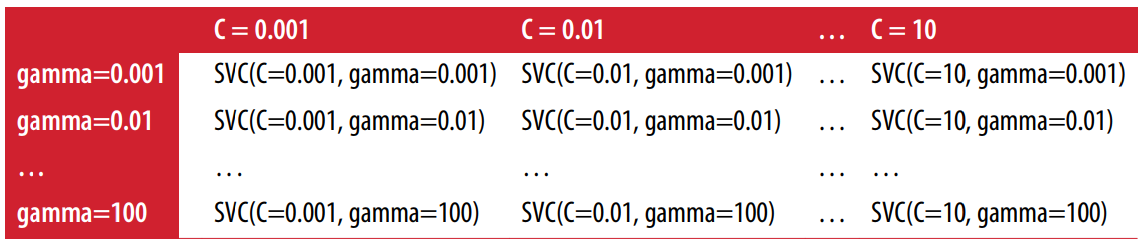
\includegraphics[scale=0.55]{Imagen_Machine/TablaGrid}
\end{figure}\label{TablaGrid} 

%  \ref{TablaGrid}


\subsubsection{Búsqueda de cuadrícula simple}\label{Gsear}

 Podemos implementar una búsqueda de cuadrícula simple al igual que para bucles sobre los dos parámetros, entrenando y evaluando un clasificador para cada combinación:  

\begin{lstlisting}%[frame=single]

In[18]:
   
   # naive grid search implementation
   from sklearn.svm import SVC
   X_train, X_test, y_train, y_test = train_test_split(
       iris.data, iris.target, random_state=0)
   print("Size of training set: {} size of test set: {}".format(
          X_train.shape[0], X_test.shape[0]))
          
   best_score = 0
   
   for gamma in [0.001, 0.01, 0.1, 1, 10, 100]:
       for C in [0.001, 0.01, 0.1, 1, 10, 100]:
           # for each combination of parameters, train an SVC
           svm = SVC(gamma=gamma, C=C)
           svm.fit(X_train, y_train)
           # evaluate the SVC on the test set
           score = svm.score(X_test, y_test)
           # if we got a better score, store the score and parameters
           if score > best_score:
              best_score = score
              best_parameters = {'C': C, 'gamma': gamma}
              
   print("Best score: {:.2f}".format(best_score))
   print("Best parameters: {}".format(best_parameters))

Out[18]:
   
    Size of training set: 112 size of test set: 38
    Best score: 0.97
    Best parameters: {'C': 100, 'gamma': 0.001}

\end{lstlisting}


\subsubsection{El peligro de sobreajustar los parámetros y el conjunto de validación}


Dado este resultado, podríamos intentar de reportar que encontramos un modelo que funciona
con un 97\% de exactitud en la data.  Sin embargo, esta afirmación podría ser demasiado optimista (o simplemente mal), por la siguiente razón: probamos  muchos parámetros diferentes y seleccionó el que tiene la mejor exactitud en el conjunto de prueba, pero esta exactitud no necesariamente es transferida a nuevos datos. Debido a que utilizamos los datos de prueba para ajustar los parámetros,  ya no podemos usarlo para evaluar lo bueno que es el modelo.  

Esta es la misma razón por la que necesitábamos dividir los datos en conjuntos de entrenamiento y prueba en primer lugar; ahora  necesitamos un conjunto independiente de datos para evaluar, uno que no se haya usado para construir el modelo.


Una forma de resolver este problema es dividir los datos nuevamente, por lo que tenemos tres conjuntos:
un conjunto de entrenamiento para construir el modelo, uno de validación (o desarrollo) para seleccionar el parámetros del modelo y el de prueba para evaluar el rendimiento de los parámetros seleccionados.  En la figura \ref{Triple}  muestra cómo se ve esto:


\begin{lstlisting}%[frame=single]

In[19]:

mglearn.plots.plot_threefold_split()


\end{lstlisting}


\begin{figure}[h!]
	\centering
	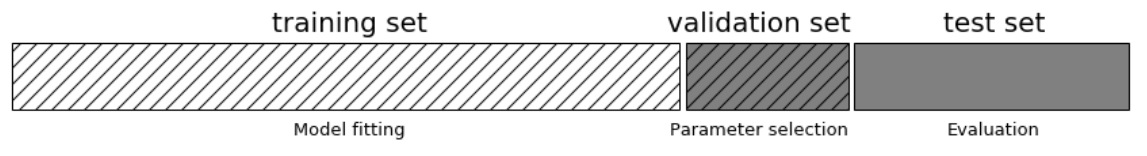
\includegraphics[scale=0.55]{Imagen_Machine/Triple}
	\caption{Una división triple-fold  de la data, en un conjunto de entrenamiento, uno de validación y el otro para prueba}
	\label{Triple}
\end{figure}


Después de seleccionar los mejores parámetros usando el conjunto de validación, podemos reconstruir un modelo usando los parámetros que encontramos, pero ahora entrenando tanto en los datos de entrenamiento como en los datos de validación. De esta manera, podemos utilizar la mayor cantidad de datos posible para construir el modelo. Esto conduce a la siguiente implementación: 

\begin{lstlisting}%[frame=single]

In[20]:

   from sklearn.svm import SVC
   # split data into train+validation set and test set
   X_trainval, X_test, y_trainval, y_test = train_test_split(
       iris.data, iris.target, random_state=0)
   # split train+validation set into training and validation sets
   X_train, X_valid, y_train, y_valid = train_test_split(
       X_trainval, y_trainval, random_state=1)
   print("Size training set: {} size validation set: {} size test set:" 
         " {}\n".format(X_train.shape[0], X_valid.shape[0], X_test.shape[0]))
         
   best_score = 0

   for gamma in [0.001, 0.01, 0.1, 1, 10, 100]:
       for C in [0.001, 0.01, 0.1, 1, 10, 100]:
       # for each combination of parameters, train an SVC
       svm = SVC(gamma=gamma, C=C)
       svm.fit(X_train, y_train)
       # evaluate the SVC on the test set
       score = svm.score(X_valid, y_valid)
       # if we got a better score, store the score and parameters
       if score > best_score:
          best_score = score
          best_parameters = {'C': C, 'gamma': gamma}
          
   # rebuild a model on the combined training and validation set,
   # and evaluate it on the test set
   svm = SVC(**best_parameters)
   svm.fit(X_trainval, y_trainval)
   test_score = svm.score(X_test, y_test)
   print("Best score on validation set: {:.2f}".format(best_score))
   print("Best parameters: ", best_parameters)
   print("Test set score with best parameters: {:.2f}".format(test_score))

Out[20]:
   
   Size of training set: 84 size of validation set: 28 size of test set: 38
   Best score on validation set: 0.96
   Best parameters: {'C': 10, 'gamma': 0.001}
   Test set score with best parameters: 0.92

\end{lstlisting}

El mejor puntaje (score) en el conjunto de validación es 96\%: ligeramente más bajo que antes, probablemente
porque usamos menos datos para entrenar el modelo ({\ttfamily X\_train} es más pequeño ahora porque dividimos la data dos veces). Sin embargo, la puntuación en el conjunto de pruebas, que realmente nos dice qué tan bien generalizamos, es aún más bajo, al 92\%. Así, que sólo podemos afirmar que la  clasificación con  nuevos datos correctamente  se de  92\% , y no del 97\%  como pensábamos antes!

La distinción entre el conjunto de entrenamiento, el de validación y el de prueba es fundamentalmente importante para aplicar métodos de aprendizaje automático en la práctica. Cualquier elección realizada en la  exactitud del conjunto de prueba  "{}fuga"{}  información del conjunto de prueba al modelo.   Por lo tanto, es importante mantener un conjunto de pruebas separado, que sólo se utilice  para la evaluación final.

 Es una buena práctica hacer todos los análisis exploratorios y la selección de modelos utilizando
la combinación de un conjunto de entrenamiento y validación, y reservar el conjunto de prueba para la evaluación  final, esto es incluso cierto para la visualización exploratoria.  Estrictamente hablando, evaluando más de un modelo en el conjunto de prueba y  eligiendo el mejor, resultaría  una estimación demasiado optimista de la exactitud del modelo.


\subsubsection{Búsqueda de cuadrícula con validación cruzada}

El método de dividir la data en los conjuntos de entrenamiento, validación y   prueba
que acabamos de ver es factible, y de uso relativamente común, pero es muy sensible  a cómo se dividen exactamente los datos. 

De la salida del fragmento de código anterior podemos ver que {\ttfamily GridSearchCV} selecciona {\ttfamily  'C': 10, y   'gamma':  0.001},   como los mejores parámetros;  mientras que la salida del código en la sección anterior selecciona a {\ttfamily 'C': 100,   y   'gamma': 0.001},  como los mejores parámetros.  

Para una mejor estimación del rendimiento de la generalización, en lugar de utilizar una única división en un conjunto de entrenamiento y  validación, podemos utilizar la validación cruzada para evaluar el rendimiento de cada combinación de parámetros. Este método puede codificarse como sigue:


\begin{lstlisting}%[frame=single]

In[21]:

   for gamma in [0.001, 0.01, 0.1, 1, 10, 100]:
       for C in [0.001, 0.01, 0.1, 1, 10, 100]:
       # for each combination of parameters,
       # train an SVC
       svm = SVC(gamma=gamma, C=C)
       # perform cross-validation
       scores = cross_val_score(svm, X_trainval, y_trainval, cv=5)
       # compute mean cross-validation accuracy
       score = np.mean(scores)
       # if we got a better score, store the score and parameters
       if score > best_score:
          best_score = score
          best_parameters = {'C': C, 'gamma': gamma}          
   # rebuild a model on the combined training and validation set
   svm = SVC(**best_parameters)
   svm.fit(X_trainval, y_trainval)

\end{lstlisting}


Para evaluar la exactitud del SVM con un ajuste particular de  C  y  gamma  mediante  la validación cruzada de 5-fold, necesitamos entrenar  36 * 5  =  180  modelos.  Como se puede imaginar, el principal inconveniente del uso de la validación cruzada es el tiempo que se tarda en entrenar todos estos modelos. 

La siguiente visualización (Figura \ref{Grid1}) ilustra cómo se selecciona el mejor parámetro en el código anterior: 


\begin{lstlisting}%[frame=single]

In[22]:

   mglearn.plots.plot_cross_val_selection()

\end{lstlisting}


	\begin{figure}[h!]
	\centering
	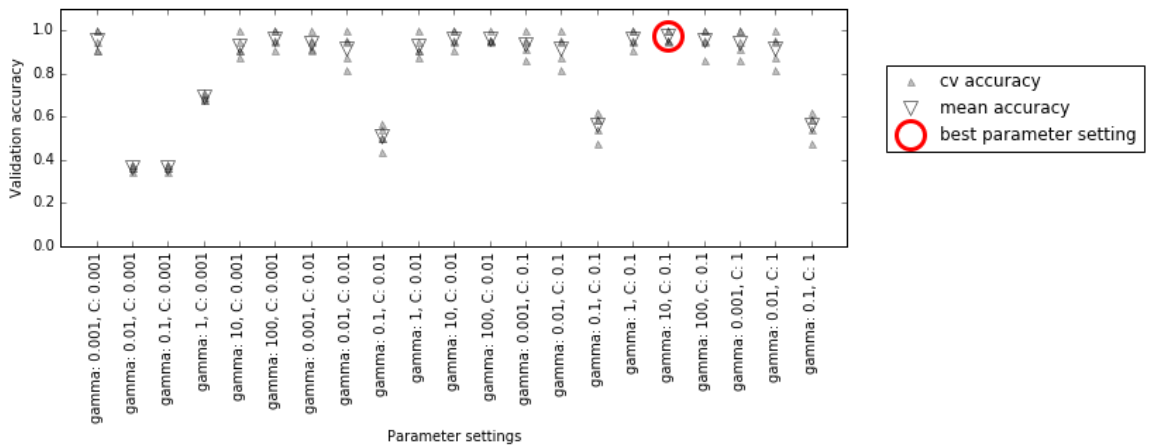
\includegraphics[scale=0.55]{Imagen_Machine/Grid1}
	\caption{Resultados de  búsqueda en cuadrícula con validación cruzada}
	\label{Grid1}
    \end{figure}


Para cada cofiguración de parámetros (sólo se muestra un subconjunto), se calculan cinco valores de exactitud, uno para cada división en la validación cruzada. Luego se calcula la exactitud media de validación para cada parámetro configuardo. Se eligen los parámetros con la mayor exactitud media de validación, marcados por el círculo.\\


\begin{minipage}[t]{0.2\textwidth}
	\centering\raisebox{\dimexpr \topskip-\height}{%
		
\includegraphics[width=\textwidth]{Imagen_Machine/Escorpion}}
\end{minipage}%\hfill
\begin{minipage}[t]{0.75\textwidth} 
	{\scriptsize		
Como hemos dicho antes, la validación cruzada es una manera de evaluar  cierto algoritmo en una 
data específica. Sin embargo, esto es  frecuentemente usado en conjunsión con métodos de búsqueda de 
parámetros como   búsqueda en cuadrícula (grid search). Por esta razón, muchas personas utilizan el término 
validación cruzada coloquialmente para referirse a la búsqueda de cuadrícula con  validación cruzada.}
\end{minipage} 
\vspace{0.5cm}

El proceso general de dividir los datos, corriendo el método grid search (la búsqueda de cuadrícula) y la  evaluación final  de los parámetros se ilustran en la Figura \ref{GridSearchCV2}:

\begin{lstlisting}%[frame=single]

In[23]:

   mglearn.plots.plot_grid_search_overview()
   
\end{lstlisting}


\begin{figure}[h!]
	\centering
	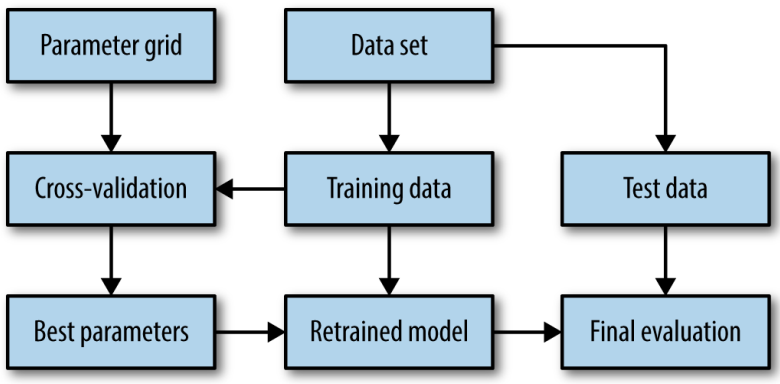
\includegraphics[scale=0.55]{Imagen_Machine/GridSearchCV2}
	\caption{Descripción general del proceso de selección de parámetros y evaluación del modelo con
		GridSearchCV}
	\label{GridSearchCV2}
\end{figure}


Debido a que  grid search   (búsqueda de cuadrícula) con validación cruzada es un método  comúnmente muy utilizado para ajustar parámetros,  {\ttfamily scikit-learn} proporciona la clase {\ttfamily GridSearchCV}, que la implementa en  forma de un estimador.
Para usar la clase {\ttfamily GridSearchCV}, primero debe especificar los parámetros que 
desea buscar utilizando un diccionario.   {\ttfamily GridSearchCV}  realizará todos los ajustes de modelo necesarios. Las claves del diccionario son los nombres de los parámetros que queremos ajustar (como se indica al construir el modelo, en este caso, C y gamma), y los valores son los parámetros que queremos probar.

Probando los valores  0.001, 0.01, 0.1, 1, 10 y 100 para  C  y  gamma se traducen en el siguiente
diccionario:


\begin{lstlisting}%[frame=single]

In[24]:

   param_grid = {'C': [0.001, 0.01, 0.1, 1, 10, 100],
                 'gamma': [0.001, 0.01, 0.1, 1, 10, 100]}
   print("Parameter grid:\n{}".format(param_grid))

Out[24]:

    Parameter grid:
    {'C': [0.001, 0.01, 0.1, 1, 10, 100], 'gamma': [0.001, 0.01, 0.1, 1, 10, 100]}

\end{lstlisting}


Ahora podemos instanciar la clase {\ttfamily  GridSearchCV} con el modelo (SVC), para buscar el parámetro
grid  ({\ttfamily  param\_grid}) y la estrategia de validación cruzada que queremos usar (por ejemplo, validación cruzada estratificada de cinco-fold):


\begin{lstlisting}%[frame=single]

In[25]:
   
   from sklearn.model_selection import GridSearchCV
   from sklearn.svm import SVC
   grid_search = GridSearchCV(SVC(), param_grid, cv=5)

\end{lstlisting}

{\ttfamily  GridSearchCV} utilizará la validación cruzada en lugar de la división en los conjuntos de entrenamiento y validación que usamos antes. Sin embargo, aún necesitamos dividir los datos en
 dos conjuntos, el de entrenamiento y   prueba, para evitar sobreajustar los parámetros:

\begin{lstlisting}%[frame=single]

In[26]:

   X_train, X_test, y_train, y_test = train_test_split(
       iris.data, iris.target, random_state=0)

\end{lstlisting}

El objeto {\ttfamily  grid\_search} que creamos se comporta como un clasificador; podemos llamar al
 métodos estándar {\ttfamily fit,  predict} y {\ttfamily  score} en él{\footnote{\scriptsize  Un estimador en {\ttfamily scikit-learn}  creado  a partir de otro estimador es llamado  meta-estimator. El {\ttfamily GridSearchCV} es el  comúnmente más  usado, pero lo veremos más adelante.}}.  
 Sin embargo, cuando llamamos {\ttfamily fit},  este corre la validación cruzada para cada combinación de parámetros que especificamos en {\ttfamily param\_grid}:

\begin{lstlisting}%[frame=single]

In[27]:

   grid_search.fit(X_train, y_train)

\end{lstlisting}

Ajustando  el objeto  {\ttfamily GridSearchCV} no sólo busca los mejores parámetros, sino que también
ajusta automáticamente un nuevo modelo en todo el conjunto de entrenamiento con los parámetros que
produjo el mejor rendimiento de validación cruzada. 

Por lo tanto, lo que sucede en {\ttfamily fit} es equivalente al resultado del código In[21] que vimos al comienzo de esta sección. La clase {\ttfamily GridSearchCV}  proporciona una interfaz muy conveniente para acceder al reentrenamiento modelo usando los métodos {\ttfamily predict}  y  {\ttfamily score}. 

Para evaluar qué tan bien  generalizar  el mejor parámetro encontrado, podemos correr {\ttfamily score} 
sobre el conjunto de prueba:

\begin{lstlisting}%[frame=single]

In[28]:

   print("Test set score: {:.2f}".format(grid_search.score(X_test, y_test)))

Out[28]:
    
    Test set score: 0.97

\end{lstlisting}

 
Seleccionando los  parámetros mediante validación cruzada, en realidad encontramos un modelo que logró
 97\% de exactitud sobre  el conjunto de prueba. Lo importante aquí, es que no se usó  el
conjunto de prueba para elegir los parámetros.

Los parámetros encontrados se anotan en el atributo {\ttfamily  best\_params\_} y la mejor exactitud de validación cruzada (la exactitud media sobre las diferentes divisiones para esta configuración de parámetros)  se almacena en {\ttfamily best\_score\_}:


\begin{lstlisting}%[frame=single]

In[29]:

   print("Best parameters: {}".format(grid_search.best_params_))
   print("Best cross-validation score: {:.2f}".format(grid_search.best_score_))

Out[29]:

    Best parameters: {'C': 100, 'gamma': 0.01}
    Best cross-validation score: 0.97

\end{lstlisting}


\begin{minipage}[t]{0.2\textwidth}
	\centering\raisebox{\dimexpr \topskip-\height}{%
		
\includegraphics[width=\textwidth]{Imagen_Machine/Zorrillo}}
\end{minipage}%\hfill
\begin{minipage}[t]{0.75\textwidth} 
	{\scriptsize		
	Nuevamente, hay que tener cuidado de no confundir {\ttfamily best\_score\_} con la generalización.
	rendimiento del modelo calculado por el método de {\ttfamily score } en el conjunto
	 de prueba. Usando el método de {\ttfamily score } (o evaluar la salida del método {\ttfamily predict})  se emplea un modelo entrenado en todo el conjunto de entrenamiento.   El atributo  {\ttfamily best\_score\_}  almacena exactitud media de la validación cruzada,  con la validación cruzada realizada en el conjunto de entrenamiento.}
\end{minipage}\\

A veces es útil tener acceso al modelo real que se encontró, por ejemplo, para ver los coeficientes o características importantes. Puede acceder al modelo con los mejores parámetros entrenados en todo el conjunto de entrenamiento utilizando el atributo {\ttfamily best\_estimator\_}:


\begin{lstlisting}%[frame=single]

In[30]:

   print("Best estimator:\n{}".format(grid_search.best_estimator_))

Out[30]:

    Best estimator:
    SVC(C=100, cache_size=200, class_weight=None, coef0=0.0,
       decision_function_shape=None, degree=3, gamma=0.01, kernel='rbf',
       max_iter=-1, probability=False, random_state=None, shrinking=True,
       tol=0.001, verbose=False)

\end{lstlisting}

Debido a que {\ttfamily grid\_search} tiene métodos de predicción y puntuación, el uso de {\ttfamily best\_estimator\_} no es necesario para hacer predicciones o evaluar el modelo.


\subsubsection{Analizando el resultado de la validación cruzada}


A menudo es útil visualizar los resultados de la validación cruzada,  para entender  cómo la  generalización del modelo depende de los parámetros que estamos buscando. Como las búsquedas de cuadrícula son muy costosos desde desde el punto de vista computacional, es una buena idea comenzar con una relación de cuadrícula relativamente robusta y pequeña.   %  gruesa   coarse  grueso
Luego podemos inspeccionar los resultados de la validación cruzada con grid search
(búsqueda de cuadrícula), y posiblemente ampliar esta búsqueda. Los resultados de una búsqueda  cuadrícula  pueden ser encontrados en el atributo {\ttfamily cv\_results\_}, que es un diccionario que almacena todos los aspectos de la búsqueda. 

Este contiene muchos detalles, como se pueden ver en el siguiente resultado, y se ve mejor
después de convertirlo en una DataFrame de {\ttfamily pandas}:


\begin{lstlisting}

In[31]:

   import pandas as pd
   # convert to DataFrame
   results = pd.DataFrame(grid_search.cv_results_)
   # show the first 5 rows
   display(results.head())

Out[31]:

       param_C  param_gamma  params                        mean_test_score
   0   0.001    0.001        {'C': 0.001, 'gamma': 0.001}       0.366
   1   0.001     0.01        {'C': 0.001, 'gamma': 0.01}        0.366
   2   0.001      0.1        {'C': 0.001, 'gamma': 0.1}         0.366
   3   0.001        1        {'C': 0.001, 'gamma': 1}           0.366
   4   0.001       10        {'C': 0.001, 'gamma': 10}          0.366

     rank_test_score split0_test_score split1_test_score split2_test_score
           
   0      22                0.375            0.347            0.363
   1      22                0.375            0.347            0.363
   2      22                0.375            0.347            0.363
   3      22                0.375            0.347            0.363
   4      22                0.375            0.347            0.363
           
          split3_test_score   split4_test_score   std_test_score
           
   0           0.363               0.380             0.011
   1           0.363               0.380             0.011
   2           0.363               0.380             0.011
   3           0.363               0.380             0.011
   4           0.363               0.380             0.011
    
\end{lstlisting}



Cada fila en el resultado corresponde a una configuración  particular del parámetro. Para 
cada conjunto, se registran los resultados de todas las divisiones de validación cruzada, así 
como la media y desviación estándar sobre todas las divisiones. 

La tabla o cuadrícula bidimensional de parámetros (C y gamma),  se visualiza mejor como un mapa
caliente, como se muestra en la figura \ref{MapaCG}.  Primero  extraemos los scores o puntajes
 promedio  de validación, luego  remodelamos o rediseñamos los puntajes o scores  para que los 
 ejes  corresponda con   C  y   gamma:

\begin{lstlisting}%[frame=single]


In[32]:

   scores = np.array(results.mean_test_score).reshape(6, 6)

   # plot the mean cross-validation scores
   mglearn.tools.heatmap(scores, xlabel='gamma', 
                         xticklabels=param_grid['gamma'],
                         ylabel='C', yticklabels=param_grid['C'],
                         cmap="viridis")

\end{lstlisting}



\begin{figure}[h!]
	\centering
	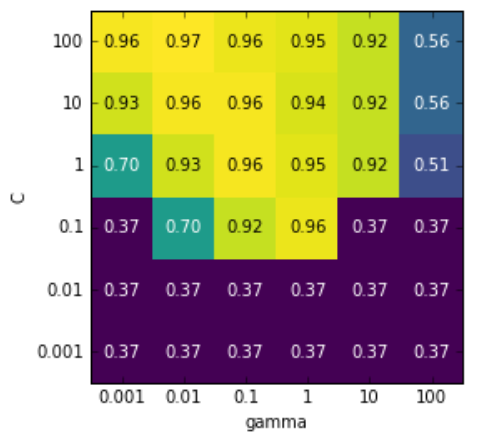
\includegraphics[scale=0.55]{Imagen_Machine/MapaCG}
	\caption{Mapa caliente  de la puntuación media de validación cruzada en función de C y gamma}
	\label{MapaCG}
\end{figure}


Cada punto en el mapa caliente corresponde a una corrida de validación cruzada, con una configuaración particular de parámetros. El color codifica la exactitud de validación cruzada, con colores claros 
 significan alta exactitud y colores oscuros que significan baja exactitud.  Se puedes ver que  SVC es muy sensible a la configuración de los parámetros.  Para muchos de los parámetros configurados, la exactitud es de alrededor del 40\%, lo cual es bastante mala; para otras configuraciones, la exactitud es alrededor del 96\%.    Podemos obtener  de este grafico  varias conclusiones. Primero, los parámetros configurados   son muy importantes para obtener un buen rendimiento. Ambos parámetros (C y gamma) son muy importantes, ya que  ajustarlos puede cambiar la exactitud del 40\% a 96\%.   Además, los rangos que seleccionamos para los parámetros son rangos en los que se ven  cambios significativos en el resultado.  También es importante tener en cuenta que los rangos para los  parámetros son lo suficientemente grandes: los valores óptimos para cada parámetro no están  en los bordes del gráfico.\\

Ahora veamos algunos gráficos (ver Figura \ref{MapaCG2}) donde el resultado es menos ideal,
porque los rangos de búsqueda no se eligieron adecuadamente:


\begin{figure}[h!]
	\centering
	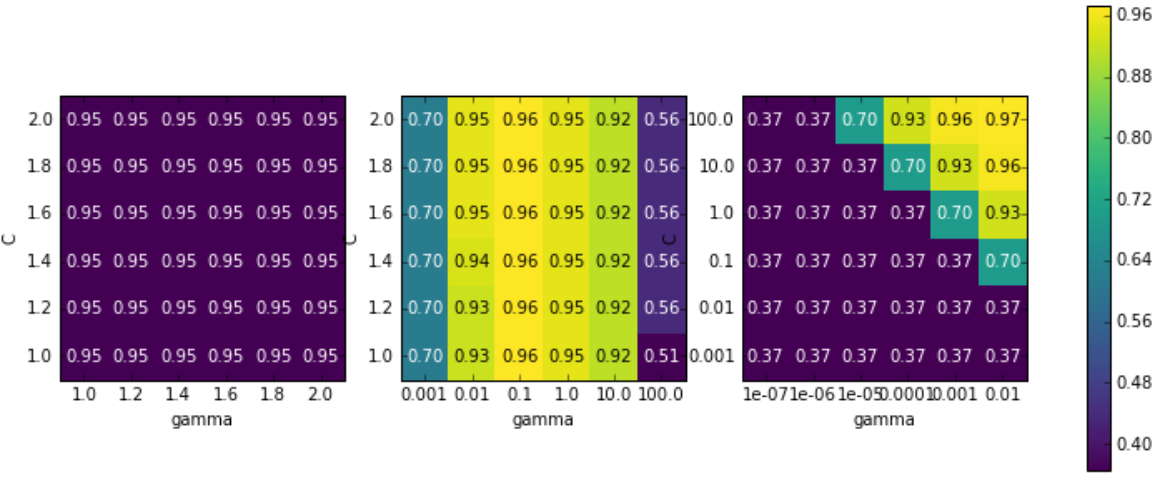
\includegraphics[scale=0.55]{Imagen_Machine/MapaCG2}
	\caption{Visualizaciones de mapas caliente de search grids mal especificadas}
	\label{MapaCG2}
\end{figure}




\begin{lstlisting}%[frame=single]

In[33]:

   fig, axes = plt.subplots(1, 3, figsize=(13, 5))
   
   param_grid_linear = {'C': np.linspace(1, 2, 6),
                        'gamma': np.linspace(1, 2, 6)}
                        
   param_grid_one_log = {'C': np.linspace(1, 2, 6),
                         'gamma': np.logspace(-3, 2, 6)}
                         
   param_grid_range = {'C': np.logspace(-3, 2, 6),
                       'gamma': np.logspace(-7, -2, 6)}
                       
   for param_grid, ax in zip([param_grid_linear, param_grid_one_log,
                              param_grid_range], axes):
       grid_search = GridSearchCV(SVC(), param_grid, cv=5)
       grid_search.fit(X_train, y_train)
       scores = grid_search.cv_results_['mean_test_score'].reshape(6, 6)
       
       # plot the mean cross-validation scores
       scores_image = mglearn.tools.heatmap(
           scores, xlabel='gamma', ylabel='C', xticklabels=param_grid['gamma'],
           yticklabels=param_grid['C'], cmap="viridis", ax=ax)
           
   plt.colorbar(scores_image, ax=axes.tolist())

\end{lstlisting}

El primer gráfico no muestra ningún cambio, con un color constante en toda la cuadrícula de parámetro.
En este caso, esto es causado por  la escala y rango incorrectos de los parámetros C y gamma.
Sin embargo, si no se observa ningún cambio en la exactitud sobre el parámetro con las diferentes
configuraciones, también podría ser que un parámetro simplemente no sea importante en lo
absoluto. Por lo general es bueno probar primero valores muy extremos, para ver si 
hay algún cambio en la exactitud como  resultado de cambiar un parámetro.\\

El segundo gráfico  muestra un patrón de rayas verticales. Esto indica que solo la configuración
del parámetro gamma hace alguna diferencia. Esto podría significar que el parámetro gamma
está buscando valores interesantes pero el parámetro C no lo está haciendo, o podría significar
que el parámetro C no es importante.\\

%   de esta frontera
El tercer gráfico muestra cambios en C y gamma. Sin embargo, podemos ver que en 
toda la parte inferior izquierda del gráfico, no pasa nada interesante. Probablemente podamos
excluir los valores muy pequeños en  futuras (grid searches)  búsquedas en la cuadrícula. 
La configuración  óptimo de parámetros  está en la parte superior derecha. Como el óptimo está en el borde de la gráfico, podemos esperar que haya algún o algunos valores mejores  más allá del borde, y podríamos querer cambiar nuestro rango de búsqueda para incluir más parámetros en esta región.\\


Ajustar los  parámetros de grid  basados   en función de las  puntuaciones (scores)  de validación cruzada está  perfectamente bien, y una buena manera de explorar la importancia de diferentes parámetros. Sin embargo, no debe probar diferentes rangos de parámetros en el conjunto de prueba final, como hemos discutido anteriormente, la evaluación del conjunto de prueba debe ocurrir sólo una vez que sabemos exactamente qué modelo queremos utilizar.


\subsubsection{Busqueda en espacios que no son cuadrículas}\label{Pagina1}




%   Search over spaces that are not grids

En algunos casos, intentar todas las combinaciones posibles de todos los parámetros como lo hace {\ttfamily  GridSearchCV}, no es una buena idea. Por ejemplo, SVC tiene un parámetro  kernel y
dependiendo de qué kernel  (o  núcleo) se elija, otros parámetros serán relevantes.    Si kernel = "{}linear"{}, el modelo es lineal y sólo se usa el parámetro C.  Si kernel = "{}rbf"{},
se utilizan los parámetros C y {\ttfamily  Gamma} (pero no otros parámetros como el grado). 
En este caso, la búsqueda en todas las combinaciones posibles de C, {\ttfamily  Gamma} y kernel no
tiene sentido:  si kernel = "{}linear"{}, no se usa {\ttfamily  Gamma} e intentar con  diferentes valores para
{\ttfamily  Gamma} sería una pérdida de tiempo. Para tratar con este tipo de parámetros "{}condicionales"{},
\: {\ttfamily GridSearchCV} permite que {\ttfamily param\_grid} sea una lista de diccionarios. Cada diccionario en el la lista se expande en una grid o cuadrícula independiente. Una posible   búsqueda de cuadrícula (grid search) que  involucre al kernel y los parámetros podrían verse así:
 
 %   would be a waste of time


\begin{lstlisting}%[frame=single]

In[34]:

   param_grid = [{'kernel': ['rbf'],
                   'C': [0.001, 0.01, 0.1, 1, 10, 100],
                   'gamma': [0.001, 0.01, 0.1, 1, 10, 100]},
                 {'kernel': ['linear'],
                  'C': [0.001, 0.01, 0.1, 1, 10, 100]}]
   print("List of grids:\n{}".format(param_grid))

Out[34]:

    List of grids:
    [{'kernel': ['rbf'], 'C': [0.001, 0.01, 0.1, 1, 10, 100],
      'gamma': [0.001, 0.01, 0.1, 1, 10, 100]},
     {'kernel': ['linear'], 'C': [0.001, 0.01, 0.1, 1, 10, 100]}]

\end{lstlisting}




En la primera cuadrícula, el parámetro del kernel siempre se establece en "{}rbf"{} 
(no es que la entrada para kernel es una lista de longitud uno), y ambos parámetros C y gamma varían. 
En la segunda cuadrícula, el parámetro del kernel se establece como  lineal, y solo C varía. Ahora
apliquemos esta búsqueda de parámetros más compleja:


\begin{lstlisting}%[frame=single]

In[35]:

   grid_search = GridSearchCV(SVC(), param_grid, cv=5)
   grid_search.fit(X_train, y_train)
   print("Best parameters: {}".format(grid_search.best_params_))
   print("Best cross-validation score: {:.2f}".format(grid_search.best_score_))

Out[35]:

    Best parameters: {'C': 100, 'kernel': 'rbf', 'gamma': 0.01}
    Best cross-validation score: 0.97

\end{lstlisting}


Echemos un vistazo a los  {\ttfamily cv\_results\_}  nuevamente. Como se esperaba, si el núcleo 
es "{}lineal"{},  entonces solo C es puede variar:

\begin{lstlisting}%[frame=single]

In[36]:

   results = pd.DataFrame(grid_search.cv_results_)
   # we display the transposed table so that it better fits on the page:
   display(results.T)

Out[36]:
\end{lstlisting}
\begin{figure}[h!]
	\centering
	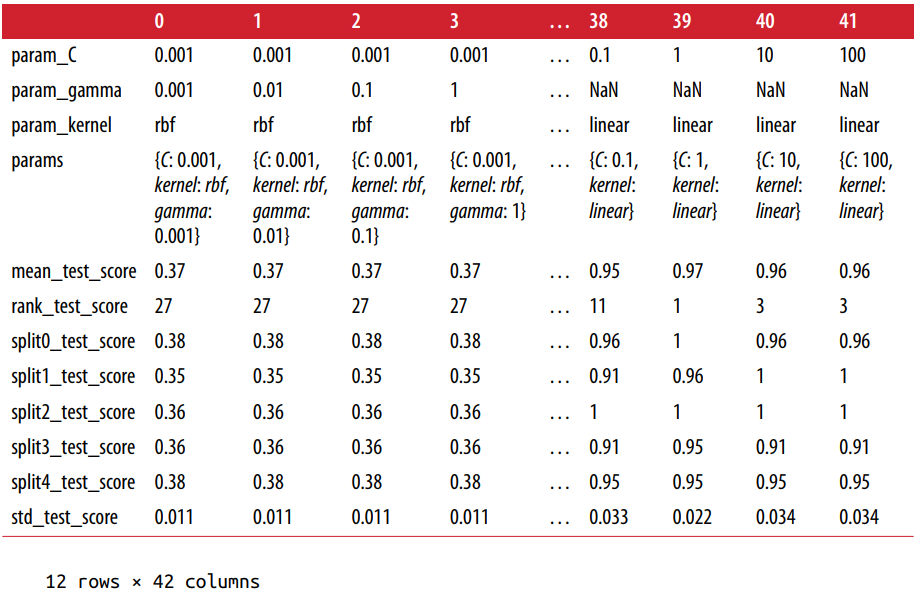
\includegraphics[scale=0.7]{Imagen_Machine/DataGrid}
	%\caption{Matriz de confusión para clasificación binaria}
	\label{DataGrid}
\end{figure}

\newpage


\subsubsection{Uso de diferentes estrategias de validación cruzada con  grid search}

De forma similar a {\ttfamily cross\_val\_score,  GridSearchCV} utiliza validación cruzada estratificada de k-fold por defecto para la clasificación y validación cruzada k-fold para la regresión.  Sin embargo, usted también puede pasar o agregar cambios a cualquier divisor de validación cruzada, como se describe en la sección \ref{VC} en la página \pageref*{VC}, como el parámetro {\ttfamily cv} en {\ttfamily GridSearchCV}. En particular, para obtener sólo una única división en un conjunto de entrenamiento y validación, se  puede usar  {\ttfamily ShuffleSplit o StratifiedShuffleSplit} con {\ttfamily n\_iter = 1}. Esto podría ser útil para datas muy grandes o modelos muy lentos.


{\subsubsection{Validación cruzada anidada}


En los ejemplos anteriores, pasamos de usar una simple  división de datos en entrenamiento,
validación y pruebas, a dividir los datos del entrenamiento y pruebas, para luego realizar la validación cruzada en el conjunto de entrenamiento. 

Pero al usar GridSearchCV  descrito anteriormente, todavía tenemos una sola división de los datos en conjuntos de entrenamiento y prueba,
lo que podría hacer que nuestros resultados sean inestables y hacernos depender demasiado de esta única división de los datos. 

Pero al usar {\ttfamily GridSearchCV} como se describió anteriormente, todavía tenemos una sola división de los datos en el conjuntos de entrenamiento y pruebas, lo que podría hacer que nuestros resultados sean inestables y hacernos depender demasiado de esta única división de los datos.

Podemos ir un paso más allá y, en lugar de dividir los datos originales en los conjuntos 
de entrenamiento y prueba una vez, use múltiples divisiones de validación cruzada. 
Esto resultará en lo que se llama validación cruzada anidada.

En la validación cruzada anidada, hay un bucle exterior sobre divisiones  de los datos en conjuntos de entrenamiento y prueba. Para cada uno de ellos, se ejecuta  una búsqueda de cuadrícula  (grid search)
(lo que puede dar como resultado mejores parámetros  diferentes  para cada división en el bucle exterior).    Luego, para cada división externa, se usa el  mejor  score  puntuación del conjunto de pruebas para la  configuración. \\

Los resultados de este procedimiento es una lista de puntajes, no es un modelo y ni un conjunto de parámetros.   Los puntajes nos dicen qué tan bien generaliza un modelo, dados los mejores parámetros encontrados  por la cuadrícula.


Como no proporciona un modelo que se pueda usar en datos nuevos, la validación cruzada anidada rara vez se usa cuando se busca un modelo predictivo para aplicar a datos futuros.
Sin embargo, puede ser útil para evaluar qué tan bien funciona un modelo dado en una data particular. 

Implementar la validación cruzada anidada en {\ttfamily scikit-learn} es sencillo.  Llamando {\ttfamily 
cross\_val\_score} con una instancia de {\ttfamily GridSearchCV} como modelo:


\begin{lstlisting}%[frame=single]

In[34]:
   
   scores = cross_val_score(GridSearchCV(SVC(), param_grid, cv=5),
                            iris.data, iris.target, cv=5)
   print("Cross-validation scores: ", scores)
   print("Mean cross-validation score: ", scores.mean())

Out[34]:

    Cross-validation scores: [ 0.967 1. 0.967 0.967 1. ]
    Mean cross-validation score: 0.98

\end{lstlisting}


El resultado de esta validación cruzada anidada se puede resumir como un modelo "{}SVC 
que puede alcanzar el 98\%  exactitud media de validación cruzada en el conjunto de
datos del iris{}"{},  nada más y nada Menos.\\

Aquí, utilizamos validación cruzada estratificada de 5-fold  tanto en el bucle interior como en el exterior. Como el {\ttfamily param\_grid} contiene 36 combinaciones de parámetros,   esto da como resultado un la enorme cantidad de  36 * 5 * 5 =  900  modelos en construcción,  lo que hace que la validación cruzada anidada sea un procedimiento muy costoso.    Aquí, utilizamos la  misma división  de validación cruzada en el bucle interior y en el externo; sin embargo, esto no es necesario y puede usar cualquier combinación
de estrategias de validación cruzada en los bucles interno y externo.

Esto puede ser un poco complicado para entender lo que está sucediendo en la simple línea  dada anteriormente, y puede ser útil visualísarlo  por bucles, como se hace en la siguiente implementación simplificada:


\begin{lstlisting}%[frame=single]

In[35]:

   def nested_cv(X, y, inner_cv, outer_cv, Classifier, parameter_grid):
       outer_scores = []
       # for each split of the data in the outer cross-validation
       # (split method returns indices)
       for training_samples, test_samples in outer_cv.split(X, y):
           # find best parameter using inner cross-validation
           best_parms = {}
           best_score = -np.inf
           # iterate over parameters
           for parameters in parameter_grid:
               # accumulate score over inner splits
               cv_scores = []
               # iterate over inner cross-validation
               for inner_train, inner_test in inner_cv.split(
                       X[training_samples], y[training_samples]):
                   # build classifier given parameters and training data
                   clf = Classifier(**parameters)
                   clf.fit(X[inner_train], y[inner_train])
                   # evaluate on inner test set
                   score = clf.score(X[inner_test], y[inner_test])
                   cv_scores.append(score)
               # compute mean score over inner folds
               mean_score = np.mean(cv_scores)
               if mean_score > best_score:
                  # if better than so far, remember parameters
                  best_score = mean_score
                  best_params = parameters
          # build classifier on best parameters using outer training set
          clf = Classifier(**best_params)
          clf.fit(X[training_samples], y[training_samples])
          # evaluate
          outer_scores.append(clf.score(X[test_samples], y[test_samples]))
       return np.array(outer_scores)

\end{lstlisting}

Ahora, vamos a correr  esta función sobre la data iris: 

\begin{lstlisting}%[frame=single]

In[36]:
   
   from sklearn.model_selection import ParameterGrid, StratifiedKFold
   scores = nested_cv(iris.data, iris.target, StratifiedKFold(5),
                      StratifiedKFold(5), SVC, ParameterGrid(param_grid))
   print("Cross-validation scores: {}".format(scores))

Out[36]:
    
    Cross-validation scores: [ 0.967 1. 0.967 0.967 1. ]

\end{lstlisting}


\subsection{Paralelismos entre validación cruzada y búsqueda de cuadrícula}
 % embarrassingly
 
Mientras se ejecuta una grid search  sobre muchos parámetros y en una data grande 
puede ser un gran reto computacionalmente y hasta difícil, también es paralelamente enrredado. 
Esto significa que construir   un modelo usando una configuración  particular de parámetro con  una división de validación cruzada específica, se puede desarrollarse completamente independientemente de las otras configuraciones de parámetros y modelos. 

Esto hace que  la grid search  búsqueda de cuadrícula y la validación cruzada sean candidatos ideales para la paralelización sobre múltiples núcleos (cores) de CPU o sobre un clúster. Puede utilizar varios núcleos en  {\ttfamily GridSearchCV} y {\ttfamily cross\_val\_score} para configurar  el parámetro
  {\ttfamily n\_jobs} como el número de núcleos de CPU que quiere usar. Puede configurar 
  {\ttfamily n\_jobs=-1} para usar todos los núcleos disponibles.



Debe tener en cuenta que {\ttfamily scikit-learn}  {\bf no permite} anidar operaciones paralelas.
Así, que si está utilizando la opción {\ttfamily n\_jobs} en su modelo (por ejemplo, un bosque aleatorio),
no puede usarlo en {\ttfamily GridSearchCV} para busquedas sobre  este modelo. 
Si la  data y el modelo son muy grande, puede que usar muchos cores núcleos que  consumen  demasiada memoria,
y debe monitorear su uso de la memoria al construir modelos grandes en paralelo.\\

También es posible paralelizar la   búsqueda de cuadrícula (grid search) y la validación cruzada en varias
máquinas en un clúster, aunque al momento de escribir esto no hay  compatible con {\ttfamily scikit-learn}.
Sin embargo, es posible utilizar el marco de trabajo de IPython en paralelo  para   búsquedas de cuadrícula paralelas, si no se le facilita  escribir el bucle  sobre los parámetros como lo hicimos 
en sección \ref{Gsear} en la página  \pageref*{Gsear}.\\

Para los usuarios de {\ttfamily   Spark}, también existe el paquete   \href{https://github.com/databricks/spark-sklearn}{\textcolor{vino}{\ttfamily spark-sklearn}}  desarrollado recientemente, que permite ejecutar una  grid search  en un clúster Spark ya establecido.







\section{Métricas de evaluación y puntuación}

Hasta ahora, hemos evaluado el rendimiento de clasificación utilizando la exactitud (accuracy) la fracción de muestras clasificadas correctamente  y el rendimiento de regresión utilizando $R^{2}$. 
 Sin embargo, estos son sólo dos de las tanta formas posibles de resumir qué tan bien funciona un modelo supervisado en una  dataset dada. En la práctica, estas métricas de evaluación pueden no ser apropiadas  para su aplicación, y es importante elegir la métrica correcta al seleccionar entre modelos y parámetros de ajuste.


\subsubsection{Mantenga el objetivo final en presente}

Al seleccionar una métrica, siempre debe tener encuenta el objetivo final de la aplicación  del aprendizaje automático.  En la práctica, generalmente estamos interesados no sólo en hacer predicciones exactas, sino tanbien en  usar estas predicciones como parte de un proceso de toma de decisiones más amplio. Antes de elegir una métrica de aprendizaje automático, debe pensar en el objetivo del alto nivel de la aplicación, a menudo denominado \emph{métrica empresarial} (business metric).   Las  consecuencias de elegir un algoritmo particular para una aplicación de aprendizaje automático se denominan {\ttfamily impacto empresarial}\footnote{\scriptsize	  Pedimos a los lectores con tendencia científica que disculpen el lenguaje comercial en esta sección. No perder de vista el objetivo final es igualmente importante en la ciencia, aunque los autores no son conscientes de una frase similar a "{}impacto empresarial"{} que se utiliza en ese ámbito.}   %    called the business metric. 

Tal vez el objetivo de alto nivel es evitar accidentes de tránsito, o disminuir el número de 
ingresos hospitalarios. También podría ser obtener más usuarios para el sitio web, o hacer
 que los usuarios gasten más dinero en su tienda.   Al elegir un  modelo o ajuste de 
 parámetros, debe elegir los valores del modelo o parámetro que más influencia más positiva 
 genera  en la métrica empresarial.  Generalmente esta tarea es difícil, ya que evaluar el impacto empresarial de un modelo en particular podría requerir ponerlo en producción en un sistema de la vida real.\\


En las primeras etapas del desarrollo, y mientras se ajustan los parámetros, generalmente no es viable
 poner el modelo en producción sólo con el próposito de prueba, debido a la alta actividad comercial
o riesgos personales que pueden estar involucrados. 

Por lo tanto, a menudo necesitamos encontrar algún procedimiento de evaluación sustituto, utilizando una métrica de evaluación que sea más fácil de calcular. \\

Escribir introducción a al objetivo de la metrica modelo\\

% Imagine evaluating the pedestrian avoidance capabilities of a self-driving car by just letting it drive around, without verifying it first; if your model is bad, pedestrians will be in trouble! Therefore we often need to find some surrogate evaluation procedure, using an evaluation metric that is easier to compute. For example, we could test classifying images of pedestrians against nonpedestrians and measure accuracy. Keep in mind that this is only a surrogate, and it pays off to find the closest metric to the original business goal that is feasible to evaluate. This closest metric should be used whenever possible for model evaluation and selection. The result of this evaluation might not be a single number—the conse‐quence of your algorithm could be that you have 10\% more customers, but each customer will spend 15\% less  —but it should capture the expected business impact of choosing one model over another.\\ Por ejemplo, podríamos probar la clasificación de imágenes de peatones contra no peatones y medir la exactitud (accuracy). Tenga en cuenta que esto es sólo un sustituto, y vale la pena encontrar la métrica más cercana al objetivo comercial original que sea factible de evaluar.  Esta métrica más cercana debe usarse siempre que sea posible para la evaluación  y selección  del modelo.   El resultado de esta evaluación podría no ser un simple número: la consecuencia  del algoritmo podría ser que tienes un 10\% más de clientes,  cada cliente gastará un 15\% menos,  debería capturar el impacto comercial esperado al elegir un modelo sobre otro.\\


En esta sección, primero discutiremos las métricas para el caso especial importante de la
clasificación  binaria, luego volvemos  a la clasificación multiclase y finalmente a la  regresión.

\subsection{Métricas para la clasificación binaria}

La clasificación binaria es posiblemente la aplicación más común y conceptualmente la aplicación más simple del aprendizaje automático en la práctica.  Sin embargo, todavía hay una serie de advertencias en la evalualuación incluso en esta  tarea simple.   Antes de sumergirnos en métricas alternativas, veamos  las formas en que la medición de la exactitud (accuracy) puede ser engañosa. Recuerda que para la clasificación binaria, frecuentemente  hablamos de una clase positiva y una clase negativa,  entendiendose que la clase positiva es la que estamos buscando.


\subsection{Tipos de errores}

Generalmente  la exactitud (accuracy) no es una buena medida del rendimiento predictivo, ya que el número de
los errores que cometemos no contienen toda la información que nos interesa. Imagine
una aplicación de pantalla para la detección anticipada de cáncer mediante una prueba automatizada. 
Si la prueba es negativa, se supondrá que el paciente está sano, mientras que si la prueba es positiva, 
el paciente se someterá a una evaluación adicional.   Aquí, llamaríamos a la prueba positiva 
(una indicación  de cáncer) como la clase positiva, y una prueba negativa a la clase negativa. No podemos
asumir que el modelo siempre funcionará perfectamente, es decir cometerá errores. Para cualquier
aplicación, debemos preguntarnos cuáles podrían ser las consecuencias de estos errores 
en el mundo real.\\

Un posible error podría ser que  un paciente sano sea clasificado como positivo, lo que lleva a
pruebas adicionales.  Esto genera  algunos costos e inconveniente para el paciente (posiblemente algo de angustia mental).  Una predicción positiva incorrecta se llama un \emph{falsa positivo}. El otro posible error ocurre cuando un paciente enfermo es clasificado como negativo, y en consecuencia no recibirá más pruebas y ni tratamiento. El cáncer no diagnosticado puede conducir a problemas de  graves de salud, e incluso podrían ser fatales.   Un error de este tipo, una precición   negativa  incorrecta: se llama  \emph{falso negativo}.   

En estadística, un \emph{falso positivo} es conocido como \emph{error tipo I}, y un \emph{falso negativo} es conocido como \emph{ error tipo II}.  Nos apegaremos  al   “{}falso positivo"{} y al "falso negativo”,  ya que son más explícitos y más fáciles de recordar. \\

En el ejemplo de diagnóstico de cáncer, es claro que queramos evitar \emph{falsos negativas} en lo más posible, mientras los falsos positivos pueden ser vistos como de una molestia menor.  Si bien este es un ejemplo particularmente drástico, la consecuencia de falsos positivos y los falsos negativos rara vez son iguales.   En aplicaciones comerciales, podría ser posible asignar valores en dólares en ambos 
tipos de errores, lo que permitiría medir el error de una predicción particular en 
dólares, en lugar de exactitud (accuracy). Esto podría ser mucho más significativo para tomar 
decisiones comerciales respecto a qué modelo utilizar.


\subsection{Datas desbalanceadas}


%  El desbalanceo de clases aparece en entornos variados como pueden ser la detección de fraude, enfermedades o spam.

Los tipos de errores juegan un papel importante cuando una de dos clases es mucho más frecuente
que el otro.  Esto es muy común en la práctica;  un buen ejemplo es la predicción de clics, donde cada punto de dato representa una "{}impresión"{}, un item que fue  mostrado al  usuario.   Este item  puede ser un anuncio, una historia relacionada o una persona a seguir en una red social. El objetivo es predecir si  se muestra un item en particular, un usuario hará clic en él (indicando que está interesado). La mayoría de las cosas que se muestran en Internet (en particular, los anuncios) no generará un clic. Es posible que deba mostrar a un usuario 100 anuncios o artículos antes de que encuentren algo lo suficientemente interesante como para hacer clic.  Esto da como resultado una data  donde por cada 99 puntos de datos "{}sin clic"{}, hay un dato  "{}cliqueados"{}; en otras palabras, el 99\% de las muestras pertenecen a la clase "{}sin clic"{}.  Una Data en cuál una  clase es mucho más frecuente que la otra, se llama desbalanceada,  o data con clases desbalanceada.  En realidad,  las datas desbalanceada es lo más común, y es raro que los eventos de interés tengan una frecuencia igual o incluso similar en la data.\\

Ahora supongamos que construimos  un clasificador con una exactitud (accuracy) del 99\% en la tarea de  predicción de clics.  ¿Qué te dice eso?  99\%  de  exactitud (accuracy) suena impresionante,  pero esto no toma en cuenta el desbalance  de clase, o de la data. Puede lograr una  exactitud (accuracy)  del 99\% sin construir un modelo de aprendizaje automático, pues al predecir siempre será  "{}sin clic"{}. 

Por otro lado, incluso con datos desbalanceados, un modelo con una exactitud (accuracy) del 99\% podría ser bastante bueno.   Sin embargo, la exactitud (accuracy) no nos permite distinguir la  constante  "{}sin clic"{}  de un modelo potencialmente  bueno.\\

Para ilustrarlo, creamos un conjunto de datos desbalanceados  9: 1,  a partir de la dataset  dígitos, por clasificación el dígito 9 contra las otras nueve clases:

   
\begin{lstlisting}%[frame=single]

In[37]:

   from sklearn.datasets import load_digits
   
   digits = load_digits()
   y = digits.target == 9
   
   X_train, X_test, y_train, y_test = train_test_split(
        digits.data, y, random_state=0)

\end{lstlisting}


Podemos usar el {\ttfamily DummyClassifier} para predecir siempre la clase mayoritaria (aquí "{}no nueve"{}) para ver cómo  puede  desinformar la  exactitud (accuracy):

\begin{lstlisting}%[frame=single]

In[38]:
   
   from sklearn.dummy import DummyClassifier
   dummy_majority = DummyClassifier(
            strategy='most_frequent').fit(X_train, y_train)
   pred_most_frequent = dummy_majority.predict(X_test)
   print("Unique predicted labels: {}".format(np.unique(pred_most_frequent)))
   print("Test score: {:.2f}".format(dummy_majority.score(X_test, y_test)))

Out[38]:
   
    Unique predicted labels: [False]
    Test score: 0.90

\end{lstlisting}

Obtuvimos una  exactitud (accuracy) cercana al 90\% sin aprender nada. Esto puede parecer llamativo, pero piénselo por un minuto. Imagina que alguien te dice que su modelo es 90\%  exacto (accuracy). Se podría pensar que hicieron un  buen trabajo. Pero dependiendo del problema, ¡eso podría ser posible prediciendo  simplemente  una clase! 

Comparemos  esto   con resultado de un clasificador real:

\begin{lstlisting}%[frame=single]

In[39]:

   from sklearn.tree import DecisionTreeClassifier
   tree = DecisionTreeClassifier(max_depth=2).fit(X_train, y_train)
   pred_tree = tree.predict(X_test)
   print("Test score: {:.2f}".format(tree.score(X_test, y_test)))

Out[39]:
   
   Test score: 0.92

\end{lstlisting}



Según la  exactitud (accuracy), el clasificador {\ttfamily DecisionTreeClassifier} es sólo un poco mejor que el predictor constante. Esto podría indicar que algo está mal con la forma en que
utilizó el clasificador  {\ttfamily DecisionTreeClassifier}, o esa medidad de exactitud aquí no es una buena.\\


Para própositos  de comparación, evalúemos dos clasificadores más, el {\ttfamily LogisticRegression}
y el {\ttfamily DummyClassifier} por defecto, que realiza predicciones aleatorias pero produce
clases con las mismas proporciones que las del conjunto de entrenamiento:


\begin{lstlisting}%[frame=single]

In[40]:
   
   from sklearn.linear_model import LogisticRegression
   
   dummy = DummyClassifier().fit(X_train, y_train)
   pred_dummy = dummy.predict(X_test)
   
   print("dummy score: {:.2f}".format(dummy.score(X_test, y_test)))
   logreg = LogisticRegression(C=0.1).fit(X_train, y_train)
   pred_logreg = logreg.predict(X_test)
   print("logreg score: {:.2f}".format(logreg.score(X_test, y_test)))

Out[40]:

   dummy score: 0.80
   logreg score: 0.98
   
\end{lstlisting}

El clasificador dummy que produce resultados aleatorios es claramente el peor los demás (según la  exactitud), mientras que {\ttfamily LogisticRegression} produce muy buenos resultados.
Sin embargo, incluso el clasificador aleatorio produce más del 80\% de  exactitud (accuracy). Esto  hace muy
 difícil juzgar cuál de estos resultados es realmente útil. El problema aquí es que la  exactitud (accuracy)  es una medida inadecuada para cuantificar el rendimiento predictivo en esta data desbalanceado.

Para el resto de este capítulo, exploraremos métricas alternativas que proporcionar una mejor orientación en la selección de modelos. En particular, nos gustaría tener métricas  que nos indiquen qué tan bueno es un modelo para  hacer predicciones  "{}más frecuentes"{}  o  predicciones aleatorias, como ellas son  calculadas   en { \ttfamily pred\_most\_frequent}  y  {\ttfamily pred\_dummy}.
 Si utilizamos una métrica para evaluar nuestros modelos, definitivamente debería ser capaz de
eliminar estas predicciones sin sentido.


\subsection{Matrices de confusión} 

Una de las formas más completas de representar el resultado de la evaluación de una clasificación 
binaria es utilizando matrices de confusión.  

Inspeccionemos las predicciones de {\ttfamily LogisticRegression} de la sección anterior usando 
 la función  {\ttfamily confusion\_matrix};   las predicciones sobre el conjunto de  pruebas  ya estan almacenadas en  {\ttfamily pred\_logreg}:


\begin{lstlisting}%[frame=single]

In[41]:

   from sklearn.metrics import confusion_matrix
   confusion = confusion_matrix(y_test, pred_logreg)
   print("Confusion matrix:\n{}".format(confusion))

Out[41]:
    
     Confusion matrix:
     [[401 2]
      [ 8 39]]
     
\end{lstlisting}


La salida de {\ttfamily confusion\_matrix} es un arreglo  2x2,  donde las filas corresponden
a las  verdaderas   clases  y las columnas concuerda con la predición de clases.    Cada  entrada cuenta la frecuencia con que una muestra que pertenece a la clase correspondiente en la fila  (en este caso es  "{}no nueve"{} y "{}nueve{}") es clasificada como la clase correspondiente en la columna.


El siguiente gráfico  (la Figura \ref{Confusion}) ilustra esta descripción:

\begin{lstlisting}%[frame=single]

In[42]:

   mglearn.plots.plot_confusion_matrix_illustration()

\end{lstlisting}


\begin{figure}[h!]
	\centering
	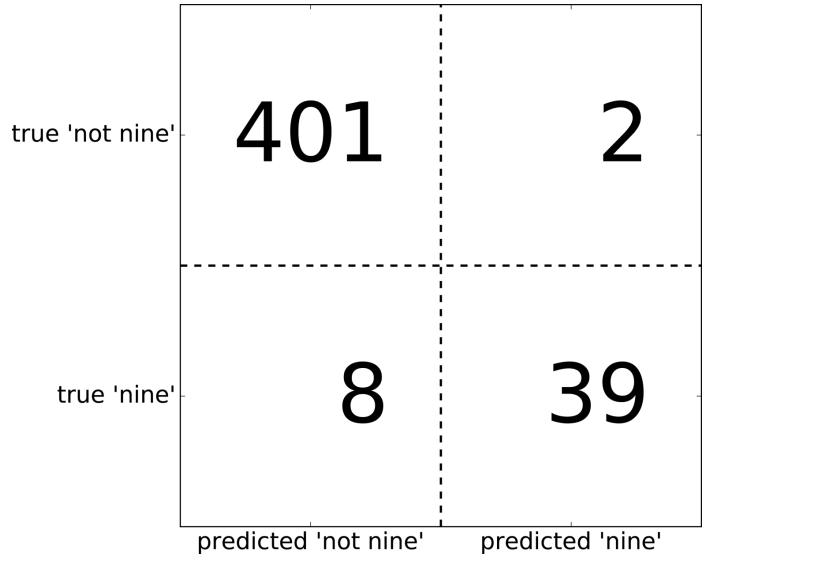
\includegraphics[scale=0.55]{Imagen_Machine/Confusion}
	\caption{Matriz de confusión de la tarea de clasificación "{}nueve vs. resto"{}}
	\label{Confusion}
\end{figure}

Las entradas en la diagonal principal\footnote{\scriptsize	  La diagonal principal de una matriz bidimensional o matriz A es A[i, i].} de la matriz de confusión corresponden a la clasificación correcta, mientras que otras entradas nos dicen cuántas muestras de una clase se clasificaron  erróneamente  como otra clase.\\

Si declaramos "{}un nueve"{} como clase positiva, podemos relacionar las entradas de la matriz de 
 confusión   con los términos falso positivo y falso negativo que presentamos anteriormente. 

Para completar el cuadro, llamamos  a las muestras clasificadas  correctamente  pertenecientes
a la clase positiva como  verdadera positiva  (true positives), y  a las muestras 
clasificadas correctamente   pertenecientes a la clase negativa como  verdadero negativos  (true negatives).
Estos términos generalmente se abrevian FP, FN, TP y TN  y  conducen a la siguiente
interpretación de  la matriz de confusión (Figura \ref{Confusion2}):





\begin{lstlisting}%[frame=single]

In[43]:

   mglearn.plots.plot_binary_confusion_matrix()

\end{lstlisting}


\begin{figure}[h!]
	\centering
	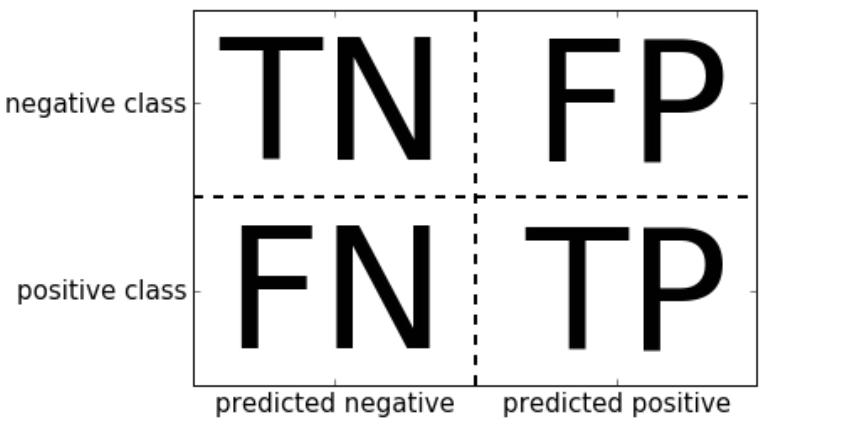
\includegraphics[scale=0.55]{Imagen_Machine/Confusion2}
	\caption{Matriz de confusión para clasificación binaria}
	\label{Confusion2}
\end{figure}



Ahora usemos la matriz de confusión para comparar los dos modelos que ajustamos anteriormente 
(los modelos simulados por  árbol de decisión y  por regresión logística):


\begin{lstlisting}%[frame=single]

In[44]:

   print("Most frequent class:")
   print(confusion_matrix(y_test, pred_most_frequent))
   print("\nDummy model:")
   print(confusion_matrix(y_test, pred_dummy))
   print("\nDecision tree:")
   print(confusion_matrix(y_test, pred_tree))
   print("\nLogistic Regression")
   print(confusion_matrix(y_test, pred_logreg))

Out[44]:

   Most frequent class:
   [[403 0]
    [ 47 0]]
   Dummy model:
   [[361 42]
    [ 43 4]]
   Decision tree:
   [[390 13]
    [ 24 23]]
   Logistic Regression
   [[401 2]
    [ 8 39]]

\end{lstlisting}


Observando la matriz de confusión, es bastante claro que algo está mal con
{\ttfamily pred\_most\_frequent}, porque siempre predice la misma clase (negativa). 
Por otro lado,  {\ttfamily pred\_dummy}  tiene un número muy pequeño de 
 verdaderos positivos  (4), que particularmente en comparación con
la cantidad de falsos negativos y falsos positivos:  hay muchos más falsos positivos
que  verdaderos positivos!   Las predicciones hechas por el árbol de decisión tienen  mucho más
sentido que las predicciones dummy, a pesar de que la exactitud era casi la misma. 
Finalmente, podemos ver que la regresión logística funciona mejor que  {\ttfamily pred\_tree} en todos los aspectos: tiene más verdaderos positivos   y  verdaderos  negativos,  y   pocos  falsos positivos y falsos negativos.    De esta comparación, está claro que sólo el árbol de decisión y la logística
la regresión da resultados razonables, y la regresión logística funciona mejor que
el árbol en todas las cuentas. 


Sin embargo, inspeccionar la matriz de confusión completa es un poco engorroso,
y aunque  ganamos   gran cantidad de información al observar todos los aspectos de la matriz,
el proceso fue muy manual y cualitativo.  Hay varias formas de resumir la información en la matriz de confusión, que discutiremos a continuación.


\subsection{Relación con la exactitud (Accuracy).} 

 Ya vimos una forma de resumir el resultado en  la matriz de confusión: calculando la exactitud,  se puede expresar como:\\

$ \text{Accuracy} = \text{exactitud} = \frac{TP+TN}{TP + TN + FP + FN} $\\


En otras palabras, la exactitud (Acuracy) es el número de predicciones correctas (TP y TN) divididas
por el número de total de las muestras (todas las entradas de la matriz de confusión resumidas).

\subsection{Precisión, Sensibilidad y f-puntuación\\ (en Inglés Precision, recall, and f-score)}
	
%	Recall =  sensitivity      %    también llamado  Tasa de Verdaderos Positivos 
 
 Hay varias otras formas de resumir la  matriz confusión, siendo unas de las más comunes la \emph{precisión} (en inglés precision)  y  la \emph{sensibilidad} (en Inglés Recall o sensitivity).\\  
 
 La  precisión  mide cuántas muestras predichas como positivas son realmente positivas:\\

$\text{Precision} =  \text{Precisión} = \frac{TP}{TP +  FP} $  \\  %  TP   TP+FP

          
La  precisión se utiliza como una métrica de rendimiento cuando el objetivo es limitar el número de falsos positivos.   Como ejemplo, imagine un modelo para predecir si un nuevo medicamento será eficaz en el tratamiento de una enfermedad en ensayos clínicos.   Por lo general los ensayos clínicos son notoriamente  costosos, y una compañía farmacéutica   solo querrá realizar un experimento si es  muy seguro de que la droga
  realmente funcionará.  Por lo tanto, es importante que el modelo no produzca muchos falsos positivos, en otras palabras, que tenga  alta precisión.   La precisión  también se conoce como    \emph{ valor predictivo positivo} (VPP).\\
 
Por otro lado,  la sensibilidad (en Inglés Recall o sensitivity),  mide cuántas de las muestras positivas son capturadas  por las predicciones positivas:\\

$ \text{Recall} = \text{sensibilidad} = \frac{TP}{TP +  FN} $  \\   %  TP   TP+FN  


La sensibilidad se utiliza como medida de rendimiento cuando necesitamos identificar todas las muestras positivas; es decir, cuando es importante evitar falsos negativos. El ejemplo del diagnóstico de cáncer dado en este capítulo, es un buen ejemplo de este caso: es importante encontrar todas las personas que están enfermas, posiblemente incluyendo  pacientes sanos en la predicción. 

Otros nombres dados a Recall son sensibilidad  o exhaustividad, \emph{tasa de éxito, o tasa de Verdaderos Positivos} (TPR).\\

Hay  una compensación entre optimizar la sensibilidad y optimizar la precisión. 
Puedes trivialmente   obtener una sensibilidad perfecta si predice que todas las muestras  que pertenecen a la clase positiva: no habrá falsos negativos y ni tampoco verdaderos negativos.   Sin embargo, prediciendo todas las muestras como  positivas darán como resultado muchos falsos
 positivos, y por lo tanto, la  precisión  debe ser muy bajo.    Por otro lado, 
 si  encuentra un modelo que predice sólo los datos individuales que son más seguros de ser positivos y 
  el resto como negativo, entonces la precisión  será perfecta (asumiendo que este punto es de hecho positivo), pero la sensibilidad será muy mala.\\


\begin{minipage}[t]{0.2\textwidth}
	\centering\raisebox{\dimexpr \topskip-\height}{%
		
\includegraphics[width=\textwidth]{Imagen_Machine/Zorrillo}}
\end{minipage}%\hfill
\begin{minipage}[t]{0.75\textwidth} 
	{\scriptsize
	La precisión y la sensibilidad son sólo dos de las tantas medidas de clasificación derivadas de TP, FP, TN y FN. Puedes encontrar un gran resumen de todas las medidas en   \href{https://en.wikipedia.org/wiki/Sensitivity_and_specificity}{\textcolor{vino}{Wikipedia} }. En la comunidad de aprendizaje automático, la precisión  y la sensibilidad son sin duda las medidas más utilizadas para la clasificación binaria, pero otras comunidades podrían utilizar otras métricas relacionadas.}
\end{minipage}\\




Si bien,  la precisión y la sensibilidad son medidas muy importantes, observar una sóla  de
ellas no le proporcionarán la imagen completa de la situación.   Una forma de resumirlos es la métrica  {\ttfamily f-score}  o  {\ttfamily f-measure},  que tiene la media armónica de la  precisión y la  sensibilidad: \\

$ F = 2 \cdot \frac{\text{ precisión} \cdot \text{sensibilidad}}{\text{ precisión}
	 + \text{sensibilidad}}  $ \\

Esta variante particular también se conoce como $f_{}1$ -puntuación  ($f_{1}$-score).  Como métrica que  toma en cuenta  la  precisión y la sensibilidad, puede ser una mejor medida que la exactitud  (accuracy) en la clasificación binaria con  data desbalanceada. 

Vamos a correr esta métrica sobre las predicciones de la data  "{}nueve vs. resto"{},  que 
se calculó  anteriormente.  Aquí, asumiremos que el "{}nueve"{} es la clase positiva (etiquetado como verdadero mientras que el resto está etiquetado como falso), por lo que la clase positiva es la clase de la minoritaria:  

\begin{lstlisting}%[frame=single]

In[45]:

   from sklearn.metrics import f1_score
   print("f1 score most frequent: {:.2f}".format(
           f1_score(y_test, pred_most_frequent)))
   print("f1 score dummy: {:.2f}".format(f1_score(y_test, pred_dummy)))
   print("f1 score tree: {:.2f}".format(f1_score(y_test, pred_tree)))
   print("f1 score logistic regression: {:.2f}".format(
           f1_score(y_test, pred_logreg)))

Out[45]:

   f1 score most frequent: 0.00
   f1 score dummy: 0.10
   f1 score tree: 0.55
   f1 score logistic regression: 0.89

\end{lstlisting}


Podemos notar dos cosas aquí. Primero, recibimos un mensaje de error para  la predicción de  {\ttfamily most\_frequent}, ya que no hubo predicciones de la clase positiva (lo que hace que el
denominador de $f$-puntuación sea cero ($f$-score)).   Además, podemos ver una distinción bastante fuerte entre
las predicciones de dummy  y las predicciones de árbol, que no estaban claras al trabajar con la
exactitud (accuracy) por sí sola. 
Usando la $f$-puntuación ($f$-score)  para la evaluación, resumimos el rendimiento predictivo de nuevo en un número.  Sin embargo, la $f$-puntuación  parece capturar nuestra intuición, de qué hace  un buen modelo mucho mejor de lo que la exactitud (accuracy) lo hizo.   No obstante, una desventaja de la $f$-puntuación,  es que es más difícil de interpretar y explicar que la exactitud.\\
 
 
Por otro lado, si se quiere un resumen más completo de las medidas de exactitud, sensibilidad y  $f$-puntaje,   puede usar la función de conveniencia {\ttfamily classification\_report}  para calcular los tres a la vez, e imprimirlos en un formato agradable:

\begin{lstlisting}%[frame=single]

In[46]:

   from sklearn.metrics import classification_report
   print(classification_report(y_test, pred_most_frequent,
                               target_names=["not nine", "nine"]))

Out[46]:

            precision   recall   f1-score  support
             
   not nine     0.90      1.00       0.94      403
   nine         0.00      0.00       0.00       47
   
   avg / total  0.80      0.90       0.85      450



\end{lstlisting}



La función {\ttfamily classification\_report} produce una línea por clase (aquí, True y False) y reporta precisión, sensibilidad y $f$-puntuación con esta clase como la clase positiva. Antes, asumimos que la clase  minoritaria "{}nueve"{}  era la clase positiva.  Si cambiamos la clase positiva a "{}no nueve"{},  podemos ver en la salida de {\ttfamily  classification\_report}  un $f$-puntaje de 0.94 para el modelo {\ttfamily most\_frequent}.  Además, para la clase "{}no nueve"{} \: tenemos una sensibilidad de 1, ya que clasificamos todas las muestras como  "{}no nueve."{}    La última columna junto a la $f$-puntuación proporciona el soporte de cada clase, lo que simplemente significa el número de muestras en esta clase de acuerdo a la verdad fundamental.\\


 
La última fila del informe de clasificación muestra una ponderación (por el número de muestras
en la clase) promedio de los números por cada clase.  Aquí hay dos informes o reportes más, uno para
el clasificador dummy y otro para la regresión logística:


\begin{lstlisting}%[frame=single]

In[47]:

   print(classification_report(y_test, pred_dummy,
                               target_names=["not nine", "nine"]))

Out[47]:

              precision    recall   f1-score   support
      
    not nine       0.90      0.92       0.91       403
       nine        0.11      0.09       0.10        47

   avg / total     0.81      0.83       0.82       450 

In[48]:

   print(classification_report(y_test, pred_logreg,
                               target_names=["not nine", "nine"]))

Out[48]:

              precision    recall   f1-score   support

   not nine        0.98      1.00        0.99      403
       nine        0.95      0.83        0.89       47

  avg / total      0.98      0.98        0.98      450


\end{lstlisting}

Como puede notar al observar los reportes, las diferencias entre el modelo dummy
y un buen modelo ya no son tan claros.  La elección de qué clase es declarada como la clase positiva tiene un gran impacto en las métricas.  Mientras que la $f$-puntuación para la clasificación dummy es 0.10  (vs. 0.89 para la regresión logística) en la clase "{}nueve"{}, para la clase "{}no nueve"{}  es 0.91 vs. 0.99, que parecen resultados razonables.  Sin embargo, al observar todos los números juntos pinta una imagen bastante exacta (accuracy), y podemos ver claramente la superioridad del modelo de regresión logística.

\subsection{Tomando en cuenta la incertidumbre}

La matriz de confusión y el reporte de clasificación proporcionan un análisis  detallado de
un conjunto particular de predicciones. Sin embargo,  las propias predicciones  ya arrojaron
una gran cantidad de información contenida en el modelo.   Como discutimos en el capítulo \ref{Cap2}, la mayoría de los clasificadores proporcionan un método  {\ttfamily decision\_function}  o  {\ttfamily predict\_proba }  para  evaluar el grado de certeza sobre las predicciones.  Hacer predicciones puede verse como un  umbral de la salida de {\ttfamily decision\_function}  o  {\tt predict\_proba }  en un cierto punto fijo; en la clasificación binaria usamos 0  para la función de decisión y  0.5  para  {\ttfamily predict\_prob}.\\

 
 A continuación se presenta un ejemplo de una tarea de clasificación binaria sobre una data desbalanceada, con 400  puntos clasificados  en la clase negativa contra 50 puntos en la clase positiva.  
 Los datos de entrenamiento se muestran a la izquierda en la Figura \ref{Impacto}. Se entrena  un modelo SVM kernel  sobre estos datos,   a la derecha de la data  de entrenamiento  se ilustra los valores en  gráficos  de la función de decisión  como un mapa caliente.  Puedes ver un círculo negro  en el  gráfico del centro en la parte superior, que  denota  el umbral de la {\ttfamily decision\_function}, que  es exactamente cero. Los puntos dentro de este   el círculo se clasificará como la clase positiva y los puntos externos como la clase negativa:\\
 
%   https://iartificial.net/precision-recall-f1-accuracy-en-clasificacion/#Terminos_es_Espanol
% Especificidad o TNR (Tasa negativa real)

\begin{lstlisting}%[frame=single]

In[49]:

   from mglearn.datasets import make_blobs
   X, y = make_blobs(n_samples=(400, 50), centers=2, cluster_std=[7.0, 2],
                     random_state=22)
   X_train, X_test, y_train, y_test = train_test_split(X, y, random_state=0)
   svc = SVC(gamma=.05).fit(X_train, y_train)

In[50]:

    mglearn.plots.plot_decision_threshold()

\end{lstlisting}


\begin{figure}[h!]
	\centering
	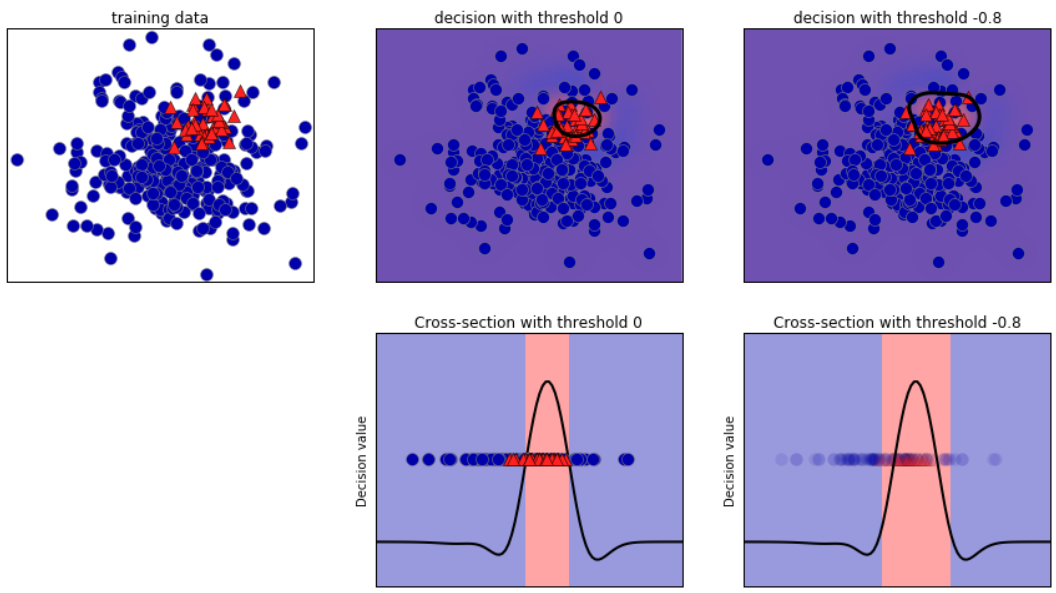
\includegraphics[scale=0.55]{Imagen_Machine/Impacto}
	\caption{Mapa caliente de la función de decisión y el impacto de la modificación del umbral de decisión}
	\label{Impacto}
\end{figure}



Podemos usar la función {\ttfamily classification\_report} para evaluar la precisión  y sensibilidad para ambas clases: 


\begin{lstlisting}%[frame=single]

In[51]:

   print(classification_report(y_test, svc.predict(X_test)))

Out[51]:

                 precision   recall   f1-score   support
                
             0        0.97     0.89       0.93       104
             1        0.35     0.67       0.46         9
       
   avg / total        0.92     0.88       0.89       113

\end{lstlisting}

Para la clase 1, obtenemos una sensibilidad  bastante pequeña, y la precisión es mixta. Debido
 a que la clase 0 es mucho más grande, el clasificador se centra en obtener la clase correcta, la 
  clase 0,  y no la clase 1 más pequeña. \\
  
Supongamos que en esta aplicación es más importante tener un valor alto de sensibilidad para la clase 1, como en el ejemplo de detección de cáncer anterior.     
  Esto significa que estamos dispuestos a arriesgar más falsos positivos (falsa clase 1) a cambio de más verdaderos positivos (lo que aumentará la sensibilidad). Las predicciones generadas por {\ttfamily svc.predict} realmente no cumplen con este requerimiento, pero podemos ajustar las predicciones para enfocarnos en una mayor sensibilidad de la clase 1, cambiando el umbral de decisión de 0. Por defecto, los puntos con un valor de {\ttfamily decision\_function}    superior a 0 se clasificarán como clase 1. 
  
  Queremos que se clasifiquen más puntos en la clase 1, por lo que necesitamos disminuir el umbral:


\begin{lstlisting}%[frame=single]

In[52]:

   y_pred_lower_threshold = svc.decision_function(X_test) > -.8

\end{lstlisting}

Veamos el reporte  de clasificación para esta predicción:


\begin{lstlisting}


In[53]:

   print(classification_report(y_test, y_pred_lower_threshold))

Out[53]:

               precision   recall   f1-score   support
               
            0       1.00     0.82       0.90       104
            1       0.32     1.00       0.49         9
            
  avg / total       0.95     0.83       0.87       113

\end{lstlisting}


Como se esperaba, la sensibilidad de la clase 1 aumentó y la precisión  disminuyó. 
Estamos ahora clasificando una región más grande del espacio como clase 1, como se ilustra en el gráfico superior derecho de Figura \ref{Impacto}.    Si evalúa  la precisión  sobre la sensibilidad o al revés, o sus datos son muy desbalanceados, cambiar el umbral de decisión es la forma más fácil de  obtener mejores  resultados.  Como {\ttfamily decision\_function}  puede  tener  rangos arbitrarios, es difícil proporcionar
una regla general sobre cómo elegir un umbral.\\


\begin{minipage}[t]{0.2\textwidth}
	\centering\raisebox{\dimexpr \topskip-\height}{%
		
\includegraphics[width=\textwidth]{Imagen_Machine/Escorpion}}
\end{minipage}%\hfill
\begin{minipage}[t]{0.75\textwidth} 
	{\scriptsize			
		Si configura un umbral, debe tener cuidado de no hacerlo usando el conjunto de prueba. Al igual que con cualquier otro parámetro, es probable que al configurar   un umbral de decisión en el conjunto de pruebas arroje resultados demasiado optimistas. En su lugar, use un conjunto de validación o validación cruzada.}
\end{minipage}\\



Elegir un umbral para  modelos que implementan el método {\ttfamily predic\_proba} puede ser
sencillo, ya que la salida de {\ttfamily predic\_proba} está en una escala fija de 0 a 1, y los modelos de probabilidad. Por defecto, el umbral de 0.5 significa que si el modelo es más del 50\%  "{}seguro"{}
que un punto es de la clase positiva, se clasificará como tal.   Aumentando el umbral significa que el modelo debe tener más confianza para tomar una decisión positiva (y menos confianza para tomar una decisión negativa).  

Trabajando con probabilidades puede ser más intuitivo que  trabajar con umbrales arbitrarios, no todos los modelos proporcionan modelos realistas de incertidumbre (un árbol de decisión que crece hasta lo más profundo es siempre 100\% seguro de sus decisiones, a pesar de que a menudo podría estar equivocado).  Esto  relaciona el concepto de calibración: un modelo calibrado es un modelo que proporciona una medidad de exactitud  de su incertidumbre.  Discutir la calibración en detalle está más allá del alcance  de  este  libro, pero puede encontrar más detalles en  el artículo \href{http://www.machinelearning.org/proceedings/icml2005/papers/079_GoodProbabilities_NiculescuMizilCaruana.pdf}{\color{vino} "{}Predicting Good Probabilities with   Supervised   Learning"{}} por   Alexandru  Niculescu-Mizil  and  Rich  Caruana.


\subsection{Precisión, sensibilidad  y curvas ROC}

% Precision-recall curves and ROC curves

Como acabamos de comentar, cambiar el umbral que se utiliza para hacer una clasificación decisión en un modelo es una forma de ajustar la compensación de precisión  y sensibilidad para una clasificación dada.
Tal vez quiera perder menos del 10\% de las muestras positivas, lo que significa que  desea una sensibilidad del  90\%.  Esta decisión depende de la aplicación, y debe ser impulsada por los objetivos del negocio.
Una vez que se configura un objetivo particular, por ejemplo, un    valor particular  de sensibilidad
  o de precisión para una clase: se puede establecer un umbral adecuadamente. Siempre es posible  configurar  un umbral  para cumplir un objetivo particular, como 90\% de sensibilidad.    Lo difícil es desarrollar un modelo  que  mantenga  una precisión  razonable con este umbral,  si  
clasifica todo como  positivo, tendrá un 100\% de sensibilidad, pero su modelo será inútil.\\

  Configurar  un requisito en un clasificador como 90\%  de  sensibilidad   con frecuencia  es llamado {\emph{ punto de operación}}.   La fijación de un {\emph{ punto de operación}}  es a menudo útil en  la configuración empresarial para dar garantías  de rendimiento a clientes u otros grupos dentro de su organización.\\

Generalmente, cuando se desarrollar un nuevo modelo, no está del todo claro cuál será el {\emph{ punto de operación}}. Por esta razón, y para entender mejor el problema de modelado, es instructivo observar  todos los umbrales posibles, o todas las posibles compensaciones entre precisión y sensibilidad a la vez. 
Esto es posible usando una herramienta llamada {\bf{curva de precisión-sensibilidad}}\index{curva de precisión-sensibilidad}. Se puede encontrar la función para calcular la curva exactitud-sensibilidad en el módulo {\ttfamily sklearn.metrics}. Necesita el etiquetado de la verdad fundamental y las incertidumbres predichas, creadas a través de {\ttfamily decision\_function} o {\ttfamily  predict\_proba}: 

\begin{lstlisting}%[frame=single]

In[54]:

   from sklearn.metrics import precision_recall_curve
   precision, recall, thresholds = precision_recall_curve(
       y_test, svc.decision_function(X_test))

\end{lstlisting}

La función {\ttfamily precision\_recall\_curve}  devuelve una lista de valores de precisión y sensibilidad para todos los umbrales posibles (todos los valores que aparecen en la función de decisión)  ordenados, para que podamos gráficar la curva, como se ve en la Figura \ref{Curva01}: 

\begin{lstlisting}%[frame=single]

In[55]:

   # Use more data points for a smoother curve
   X, y = make_blobs(n_samples=(4000, 500), centers=2, cluster_std=[7.0, 2],
                     random_state=22)
   X_train, X_test, y_train, y_test = train_test_split(X, y, random_state=0)
   svc = SVC(gamma=.05).fit(X_train, y_train)
   precision, recall, thresholds = precision_recall_curve(
       y_test, svc.decision_function(X_test))
   # find threshold closest to zero
   close_zero = np.argmin(np.abs(thresholds))
   plt.plot(precision[close_zero], recall[close_zero], 'o', markersize=10,
            label="threshold zero", fillstyle="none", c='k', mew=2)
            
   plt.plot(precision, recall, label="precision recall curve")
   plt.xlabel("Precision")
   plt.ylabel("Recall")

\end{lstlisting}


\begin{figure}[h!]
	\centering
	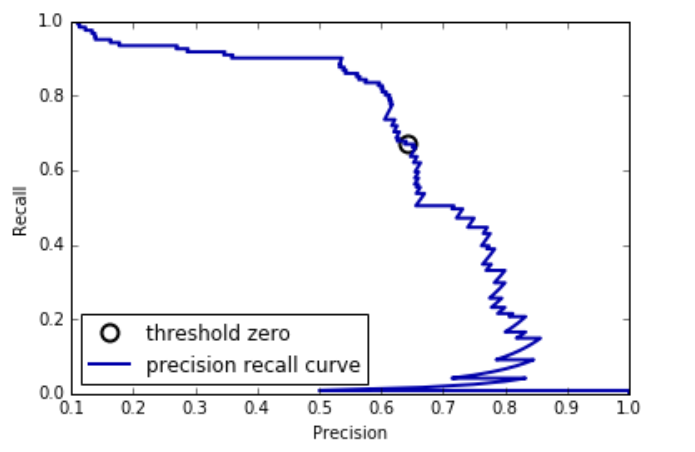
\includegraphics[scale=0.55]{Imagen_Machine/Curva01}
	\caption{Curva de precisión y sensibilidad   para SVC (gamma=0.05)}
	\label{Curva01}
\end{figure}

Cada punto a lo largo de la curva en la Figura \ref{Curva01}  corresponde a un posible umbral de la
{\ttfamily decisión\_función}. Podemos ver, por ejemplo, que se puede  lograr una  sensibilidad de 0.4 en una  precisión de aproximadamente 0,75.  El círculo negro marca el punto que corresponde a un umbral
 de 0, por defecto el umbral  para la {\ttfamily decisión\_función}. Este punto es la compensación que
se elige al llamar al método de predicción.


Cuanto más cerca se mantenga una curva de la esquina superior derecha, mejor será el clasificador. Un punto en la esquina superior derecha significa alta precisión y alta sensibilidad para el mismo umbral. 
La curva comienza en la esquina superior izquierda, corresponde  a un umbral muy bajo, clasificando
todo como la clase positiva.  Al elevar el umbral, la curva se mueve hacia una alta  precisión, pero también baja la sensibilidad. Subiendo el umbral cada vez más, llegamos a una  situación en la que la mayoría de los puntos  clasificados como positivos, son verdaderos positivos, lo que conduce a una muy alta precisión  pero menor sensibilidad.  Cuanto más el modelo mantiene  alta la sensibilidad  a medida que la precisión sube, lo mejor.


Si observamos   esta curva en particular un poco más, podemos ver que con este modelo es posible
 obtener una precisión   alrededor de 0,5 con una sensibilidad muy alta. Si queremos  mayor precisión, tenemos que sacrificar un poco de sensibilidad. En otras palabras,  la curva es relativamente
plana a la izquierda, lo que significa que la sensibilidad no baja mucho cuando necesitamos
mayor precisión. Para una precisión mayor a 0.5, cada ganancia en precisión nos cuesta un buena cantidad de  sensibilidad. \\
 
Los diferentes clasificadores pueden funcionar bien en diferentes partes de la curva, es decir, en diferentes puntos de operación.    Comparemos el modelo SVM  con el modelo de bosque aleatorio entrenados  en el mismo conjunto de datos.   El  {\ttfamily RandomForestClassifier} no tiene  {\ttfamily decision\_function}, sólo {\ttfamily  predic\_proba}.     La función {\ttfamily precision\_recall\_curve} espera como su segundo argumento   una medida de certeza para la clase positiva (clase 1), así que pasamos la probabilidad de que una muestra sea de clase 1, es decir, {\ttfamily rf.predict\_proba (X\_test)[:, 1]}.   El valor por defecto del umbral para {\ttfamily predic\_proba}  en la clasificación binaria es 0.5, entonces este es el punto marcado en la curva (ver Figura \ref{Curva02}):



\begin{lstlisting}%[frame=single]

In[56]:

   from sklearn.ensemble import RandomForestClassifier
   
   rf = RandomForestClassifier(n_estimators=100, random_state=0, 
                               max_features=2)
   rf.fit(X_train, y_train)
   
   # RandomForestClassifier has predict_proba, but not decision_function
   precision_rf, recall_rf, thresholds_rf = precision_recall_curve(
   y_test, rf.predict_proba(X_test)[:, 1])
   
   plt.plot(precision, recall, label="svc")
   
   plt.plot(precision[close_zero], recall[close_zero], 'o', markersize=10,
            label="threshold zero svc", fillstyle="none", c='k', mew=2)
   
   plt.plot(precision_rf, recall_rf, label="rf")
   
   close_default_rf = np.argmin(np.abs(thresholds_rf - 0.5))
   plt.plot(precision_rf[close_default_rf], recall_rf[close_default_rf], '^',
            c='k',  markersize=10, label="threshold 0.5 rf", 
            fillstyle="none", mew=2)            
   plt.xlabel("Precision")
   plt.ylabel("Recall")
   plt.legend(loc="best")

\end{lstlisting}



\begin{figure}[h!]
	\centering
	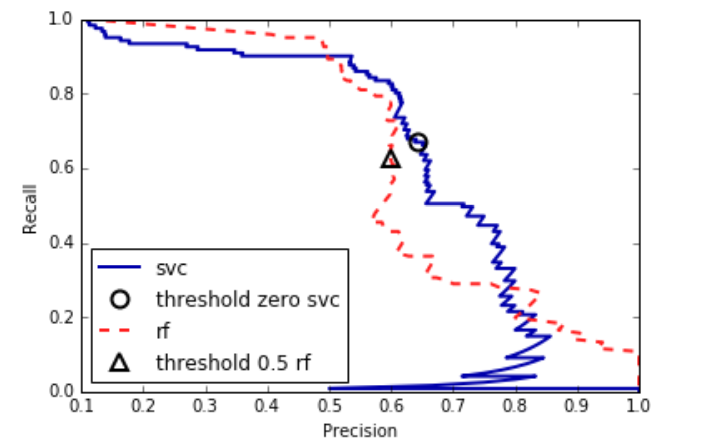
\includegraphics[scale=0.55]{Imagen_Machine/Curva02}
	\caption{Comparación de la  curvas de precisión-sensibilidad del SVM y bosque aleatorio}
	\label{Curva02}
\end{figure}


A partir de la gráfica de comparación podemos ver que el bosque aleatorio funciona mejor en los extremos, para una muy alta sensibilidad  o requisitos de precisión muy altos. Alrededor del  medio el SVM funciona mejor (aproximadamente una precisión = 0,7). Si sólo hubiéramos observado la $f_{1}$-puntuación  para comparar el rendimiento general, nos habríamos perdido estas sutilezas. La $f_{1}$-puntuación sólo captura un punto en la curva de precisión-sensibilidad, el que viene dado por el umbral por defecto:


\begin{lstlisting}%[frame=single]

In[57]:

   print("f1_score of random forest: {:.3f}".format(
          f1_score(y_test, rf.predict(X_test))))
   print("f1_score of svc: {:.3f}".format(
          f1_score(y_test, svc.predict(X_test))))

Out[57]:
   
    f1_score of random forest: 0.610
    f1_score of svc: 0.656

\end{lstlisting}



Comparando dos curvas de precisión-sensibilidad  proporciona gran cantidad de información detallada, pero es un proceso bastante manual. Para  comparar modelos automáticas, puede ser que queremos  resumir la información contenida en la curva, sin limitarnos a un umbral en particular   o  al  puntos de operación.
Una forma particular de resumir la curva precisión-sensibilidad,  es calculando la integral o el área bajo la curva de la curva de precisión-sensibilidad, también conocida como la \emph{precisión media}\footnote{\scriptsize	  Existen algunas diferencias técnicas menores entre el área bajo la curva de precisión-sensibilidad y la   precisión media. Sin embargo, esta explicación transmite la idea general.}. 
 Se puede usar la función {\ttfamily average\_precision\_score}  para calcular la precisión media.
Debido a que necesitamos calcular la curva ROC y considerar varios umbrales, el resultado de {\ttfamily decision\_function} o  {\ttfamily predict\_proba}  debe pasarse a {\ttfamily average\_precision\_score}, no el resultado de {\ttfamily predict}:



\begin{lstlisting}%[frame=single]

In[58]:
   
   from sklearn.metrics import average_precision_score
   ap_rf = average_precision_score(y_test, rf.predict_proba(X_test)[:, 1])
   ap_svc = average_precision_score(y_test, svc.decision_function(X_test))
   print("Average precision of random forest: {:.3f}".format(ap_rf))
   print("Average precision of svc: {:.3f}".format(ap_svc))

Out[58]:
   
    Average precision of random forest: 0.666
    Average precision of svc: 0.663

\end{lstlisting}


Al promediar todos los umbrales posibles, vemos que el bosque aleatorio y SVC
funcionan de manera similar, con el bosque aleatorio incluso un poco más adelante. Esto es muy diferente al  resultado que obtuvimos de {\ttfamily f1\_score} anteriormente.   Porque la precisión promedio es el área bajo una curva que va de 0 a 1, este siempre devuelve un valor  entre 0 (peor) y 1 (mejor). La precisión promedio de un clasificador que  asigna  {\ttfamily decision\_function}  al azar es la fracción de muestras positivas en el conjunto de datos.  


\subsubsection{Característica Operativa del Receptor (ROC) y el área bajo la curva  (AUC)}

% curva (ROC) de la característica operativa del receptor (n.f.)
%  recall (denominado igualmente sensibilidad o exhaustividad) 

Hay otra herramienta que se usa comúnmente para analizar el comportamiento de los clasificadores con
umbrales diferentes: la curva de característica operativa del receptor o la curva ROC. 

Similar a la curva de precisión-sensibilidad, la curva ROC considera todos los umbrales posibles para un clasificador dado, pero en lugar de reportar la precisión y sensibilidad, muestra la tasa de falsos positivos (false positive rate,  FPR) contra la tasa de verdaderos positivos (true positive rate, TPR). Recuerde  que la tasa verdaderos positivos  es simplemente otro nombre para la sensibilidad, mientras que la tasa falsos positivos es la fracción o tasa de falsos positivos de todas las muestras negativas:\\

$  FPR = \frac{FP }{FP+TN} $\\

%  Tasa de falsos positivos (FPR) se define de la siguiente manera:


La curva ROC puede calcularse utilizando la función {\ttfamily roc\_curve} (véase la figura \ref{Curva03}):

\begin{lstlisting}%[frame=single]

In[59]:

   from sklearn.metrics import roc_curve 
   fpr, tpr, thresholds = roc_curve(y_test, svc.decision_function(X_test))
   
   plt.plot(fpr, tpr, label="ROC Curve")
   plt.xlabel("FPR")
   plt.ylabel("TPR (recall)")
   # find threshold closest to zero
   close_zero = np.argmin(np.abs(thresholds))
   plt.plot(fpr[close_zero], tpr[close_zero], 'o', markersize=10,
            label="threshold zero", fillstyle="none", c='k', mew=2)
   plt.legend(loc=4)

\end{lstlisting}


\begin{figure}[h!]
	\centering
	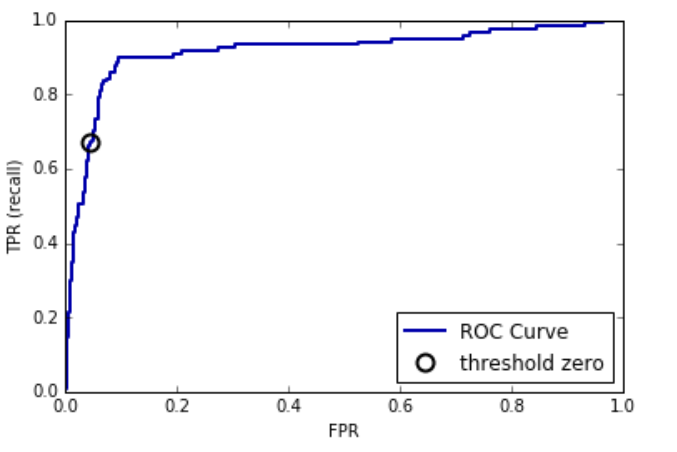
\includegraphics[scale=0.55]{Imagen_Machine/Curva03}
	\caption{Curva ROC para SVM}
	\label{Curva03}
\end{figure}


Para la característica operativa del receptor (ROC), la curva ideal está cerca de la parte superior izquierda: queremos  un  clasificador que produzca una alta sensibilidad  manteniendo una baja tasa de falsos positivos. 

En comparación con el umbral por defecto de 0, la curva muestra que podemos lograr una  sensibilidad significativamente mayor (alrededor de 0,9), mientras que sólo aumenta el FPR ligeramente.

El punto más cercano a la parte superior izquierda podría ser un mejor punto de operación que el elegido por defecto. Una vez más, tenga en cuenta que la elección de un umbral no debe hacerse en el conjunto de pruebas, sino en un conjunto de validación separado.
  
  %  puntos  operativo

En la Figura \ref{Curva04} se presenta  una comparación entre el bosque aleatorio y la SVM utilizando curvas ROC:

\begin{lstlisting}%[frame=single]

In[60]:

   from sklearn.metrics import roc_curve
   fpr_rf, tpr_rf, thresholds_rf = roc_curve(
            y_test, rf.predict_proba(X_test)[:, 1])
   
   plt.plot(fpr, tpr, label="ROC Curve SVC")
   plt.plot(fpr_rf, tpr_rf, label="ROC Curve RF")
   
   plt.xlabel("FPR")
   plt.ylabel("TPR (recall)")
   plt.plot(fpr[close_zero], tpr[close_zero], 'o', markersize=10,
            label="threshold zero SVC", fillstyle="none", c='k', mew=2)
   close_default_rf = np.argmin(np.abs(thresholds_rf - 0.5))
   plt.plot(fpr_rf[close_default_rf], tpr[close_default_rf], '^',
            markersize=10, label="threshold 0.5 RF", fillstyle="none",
            c='k', mew=2)
   
   plt.legend(loc=4)

\end{lstlisting}


\begin{figure}[h!]
	\centering
	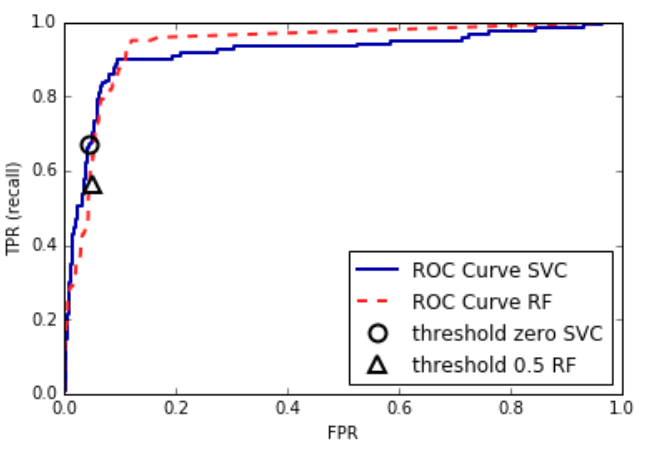
\includegraphics[scale=0.55]{Imagen_Machine/Curva04}
	\caption{Comparación de curvas ROC para SVM y bosque aleatorio}
	\label{Curva04}
\end{figure}


En cuanto a la curva precisión-sensibilidad, frecuentemente se quiere resumir la curva ROC usando 
un sólo número, el {\bf área bajo la curva} (esto se conoce comúnmente como AUC, y se entiende que la 
curva en cuestión es la curva ROC). Podemos comparar el área bajo la curva ROC usando la función
 {\ttfamily roc\_auc\_score}:

%Cuando se utilizan unidades normalizadas, el área bajo la curva (a menudo denominada simplemente AUC) es igual a la probabilidad de que un clasificador clasifique una instancia positiva elegida aleatoriamente por encima de una instancia negativa elegida aleatoriamente (asumiendo que 'positivo' clasifica por encima de ' negativo')

\begin{lstlisting}%[frame=single]

In[61]:

   from sklearn.metrics import roc_auc_score
   rf_auc = roc_auc_score(y_test, rf.predict_proba(X_test)[:, 1])
   svc_auc = roc_auc_score(y_test, svc.decision_function(X_test))
   print("AUC for Random Forest: {:.3f}".format(rf_auc))
   print("AUC for SVC: {:.3f}".format(svc_auc))

Out[61]:

    AUC for Random Forest: 0.937
    AUC for SVC: 0.916

\end{lstlisting}

%   Características de funcionamiento del receptor (ROC) y AUC 
%   Receiver operating characteristics (ROC) and AUC There 
%   Características operativas del receptor (ROC) y AUC

Comparando el bosque aleatorio y SVM usando el puntaje AUC, encontramos que el bosque aleatorio
funciona  mejor que el SVM. Recordemos eso porque la precisión media
 es el área bajo una curva que va de 0 a 1, la precisión media siempre retorna 
un valor entre 0 (peor) y 1 (mejor). La predicción aleatoria siempre produce un AUC
de 0.5, no importa qué tan desbalanceados  estén las clases en una dataset. 
Esto hace que AUC sea una  métrica mucho mejor para problemas de clasificación desbalanceada que la exactitud.  Las AUC puede interpretarse como una evaluación de la clasificación de muestras positivas. Es equivalente a la probabilidad de que un punto elegido al azar de la clase positiva tenga una puntuación más alta  según el clasificador que un punto elegido al azar de la clase negativa.   Así, un  AUC perfecto de 1 significa que todos los puntos positivos tienen una puntuación más alta que todos los negativos puntos.

Para problemas de clasificación con clases desbalanceadas, usando AUC para el modelo
 seleccinado suele ser mucho más significativa que usar la exactitud.

Volvamos al problema que estudiamos anteriormente de clasificar todos los nueves en dataset de dígitos
 versus todos los demás dígitos.  Clasificaremos la dataset con un SVM con tres diferentes
configuraciones  del ancho de banda del kernel, gamma (ver Figura \ref{Curva05}):


\begin{lstlisting}%[frame=single]

n[62]:

   y = digits.target == 9
   
   X_train, X_test, y_train, y_test = train_test_split(
       digits.data, y, random_state=0)
   
   plt.figure()
                    #  o   [1, 0.05, 0.01]:
   for gamma in [1, 0.1, 0.01]:         
       svc = SVC(gamma=gamma).fit(X_train, y_train)
       accuracy = svc.score(X_test, y_test)
       auc = roc_auc_score(y_test, svc.decision_function(X_test))
       fpr, tpr, _ = roc_curve(y_test , svc.decision_function(X_test))
       print("gamma = {:.2f} accuracy = {:.2f} AUC = {:.2f}".format(
             gamma, accuracy, auc))
   plt.plot(fpr, tpr, label="gamma={:.3f}".format(gamma))
   plt.xlabel("FPR")
   plt.ylabel("TPR")
   plt.xlim(-0.01, 1)
   plt.ylim(0, 1.02)
   plt.legend(loc="best")

Out[62]:

   gamma = 1.00 accuracy = 0.90 AUC = 0.50
   gamma = 0.1 accuracy = 0.90 AUC = 0.96
   gamma = 0.01 accuracy = 0.90 AUC = 1.00

\end{lstlisting}



\begin{figure}[h!]
	\centering
	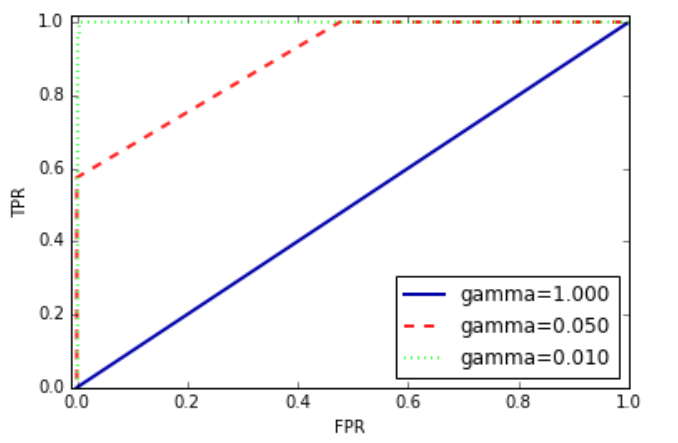
\includegraphics[scale=0.55]{Imagen_Machine/Curva05}
	\caption{curvas ROC para  SVMs con diferentes  configuraciones de gamma}
	\label{Curva05}
\end{figure}


La exactitud en las tres configuraciones de gamma es la misma, 90\%. Esto podría ser lo mismo
como un rendimiento casual, o tal vez no. Sin embargo,  observando las AUC y la curva  correspondiente,   
 vemos una clara distinción entre los tres modelos.  Con gamma = 1.0,
el AUC está realmente en el nivel de oportunidad o chance, lo que significa que la salida del {\ttfamily decision\_function} es tan buena como el aleatorio.  Con gamma = 0.01, el rendimiento mejora drásticamente de un AUC de 0.5 a 0.96. Finalmente, con gamma = 0.01, obtenemos un AUC perfecto igual a  1.0.   Eso significa que Todos los puntos positivos se clasifican más alto que todos los puntos negativos de acuerdo con la función de decisión. En otras palabras, con el umbral correcto, este modelo puede clasificar los datos perfectamente\footnote{\scriptsize  Observando la curva para {\ttfamily gamma=0.01} en detalle, se puede ver un pequeño giro cerca de la parte superior izquierda. Esto significa que al menos un punto no fue clasificado correctamente. La AUC de 1.0 es una consecuencia del redondeo al segundo punto decimal.}! 
Conociendo esto, podemos ajustar el umbral en este modelo y obtener excelentes predicciones.
Si solo hubiéramos usado la exactitud, nunca habríamos descubierto esto.  \\

Por esta razón, recomendamos usar AUC al evaluar modelos sobre dataset desbalanceadas.  Tenga en cuenta que AUC no utiliza el umbral predeterminado; sin embargo, puede ser necesario ajustar el umbral de decisión para obtener resultados de clasificación útiles a partir de un modelo con un AUC alto.

\subsection{Métricas para la clasificación multiclase}

Ahora que hemos discutido la evaluación de las tareas de clasificación binaria en profundidad, vamos a
pasar a las métricas para evaluar la clasificación multiclase. Básicamente, todas las métricas para
la clasificación multiclase se deriva de las métricas de clasificación binaria, pero promediado
sobre todas las clases.

La exactitud para la clasificación multiclase se define de nuevo como la fracción de ejemplos correctamente clasificados. Y de nuevo, cuando las clases están desbalanceadas, la exactitud no es una gran medida de evaluación. Imagine un problema de clasificación con tres clases con 85\% de puntos pertenecientes a la clase A, 10\% pertenecientes a la clase B y 5\% pertenecientes a la clase C.  ¿Qué significa ser 85\% exacto en este conjunto de datos? En general, los resultados de clasificación multiclase son más difíciles de entender que los resultados de clasificación binaria. Aparte de la exactitud, las dos herramientas más comunes son la matriz de confusión y el reporte de clasificación que vimos en el caso binario en la sección anterior. Vamos a aplicar estos dos métodos de evaluación detallada en la tarea de clasificar los 10  diferentes dígitos manuscritos en en la dataset de dígitos.



\begin{lstlisting}%[frame=single]

In[63]:

   from sklearn.metrics import accuracy_score
   X_train, X_test, y_train, y_test = train_test_split(
       digits.data, digits.target, random_state=0)
   lr = LogisticRegression().fit(X_train, y_train)
   pred = lr.predict(X_test)
   print("Accuracy: {:.3f}".format(accuracy_score(y_test, pred)))
   print("Confusion matrix:\n{}".format(confusion_matrix(y_test, pred)))

Out[63]:

    Accuracy: 0.953
    Confusion matrix:
    [[37 0 0 0 0 0 0 0 0 0]
     [ 0 39 0 0 0 0 2 0 2 0]
     [ 0 0 41 3 0 0 0 0 0 0]
     [ 0 0 1 43 0 0 0 0 0 1]
     [ 0 0 0 0 38 0 0 0 0 0]
     [ 0 1 0 0 0 47 0 0 0 0]
     [ 0 0 0 0 0 0 52 0 0 0]
     [ 0 1 0 1 1 0 0 45 0 0]
     [ 0 3 1 0 0 0 0 0 43 1]
     [ 0 0 0 1 0 1 0 0 1 44]]

\end{lstlisting}


El modelo tiene una exactitud del 95,3\%, lo que ya nos dice que lo estamos haciendo bastante bien. La matriz de confusión nos proporciona un poco más de detalle. En cuanto al caso binario, cada fila corresponde a una verdadera etiqueta, y cada columna corresponde a una etiqueta predicha. Puedes encontrar  visualización  más atractiva en la Figura \ref{ConfuM1}:


\begin{lstlisting}%[frame=single]

In[64]:

   scores_image = mglearn.tools.heatmap(
   confusion_matrix(y_test, pred), xlabel='Predicted label',
   ylabel='True label', xticklabels=digits.target_names,
   yticklabels=digits.target_names, cmap=plt.cm.gray_r, fmt="%d")
   plt.title("Confusion matrix")
   plt.gca().invert_yaxis()

\end{lstlisting}


\begin{figure}[h!]
	\centering
	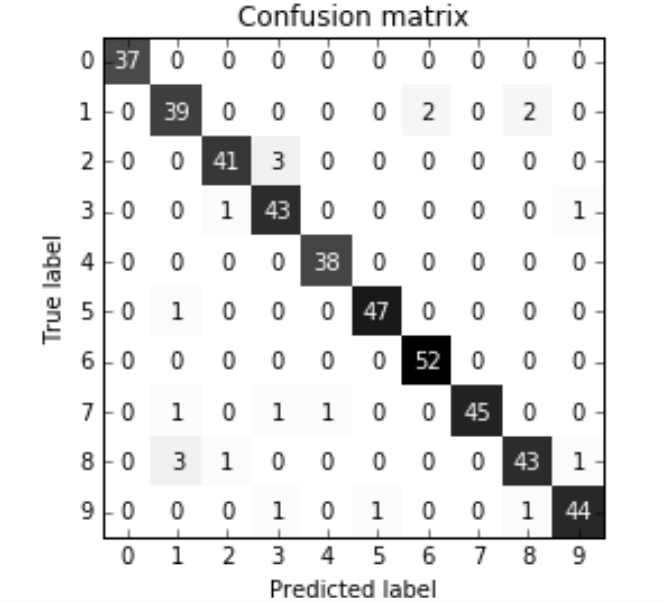
\includegraphics[scale=0.55]{Imagen_Machine/ConfuM1}
	\caption{Matriz de confusión para la tarea de clasificación de 10 dígitos}
	\label{ConfuM1}
\end{figure}

Para la primera clase, el dígito 0, hay 37 muestras en la clase, y todas estas muestras
 se clasificaron como clase 0 (no hay falsos negativos para la clase 0). Podemos ver eso
porque todas las demás entradas en la primera fila de la matriz de confusión son 0.
También podemos ver que ningún otro dígito se clasificó erróneamente como 0, porque todas las demás entradas en la primera columna de la matriz de confusión son 0 (no hay falsos positivos para la clase 0).
Sin embargo, algunos dígitos se confundieron con otros, por ejemplo, el dígito 2 (tercera fila),
tres de los cuales fueron clasificados como el dígito 3 (cuarta columna). También había un dígito
3 que se clasificó como 2 (cuarta fila, tercera columna) y un dígito 8 que se clasificó
como 2 (novena fila, tercera columna).

Con la función {\ttfamily classification\_report}, podemos calcular la precisión, sensibiidad,
y $f$-puntaje  para cada clase:


\begin{lstlisting}%[frame=single]

In[65]:

   print(classification_report(y_test, pred))

Out[65]:

               precision   recall   f1-score   support
    
             0      1.00     1.00       1.00        37
             1      0.89     0.91       0.90        43
             2      0.95     0.93       0.94        44
             3      0.90     0.96       0.92        45
             4      0.97     1.00       0.99        38
             5      0.98     0.98       0.98        48
             6      0.96     1.00       0.98        52
             7      1.00     0.94       0.97        48
             8      0.93     0.90       0.91        48
             9      0.96     0.94       0.95        47
             
   avg / total 0.95 0.95 0.95 450

\end{lstlisting}

Como era de esperar, la precisión y la sensibilidad son  perfectas, 1 para la clase 0, ya que no hay confusiones con esta clase. Por otro lado, para la clase 7,  la precisión es 1 porque no hay otra
la clase  clasificada  erróneamente como 7, mientras que para la clase 6 no hay falsos negativos, por lo que
el sensibilidad es 1. También podemos ver que el modelo tiene dificultades particulares con las clases 8
y la 3.

La métrica más utilizada para dataset desbalanceados  en la configuración de multiclase es
la versión multiclase del $f$-puntaje ($f$-score). La idea detrás del $f$-puntaje  multiclase es 
calcular un $f$-puntaje binario por clase, siendo esa clase la clase positiva y las otras
clases componen las clases negativa.

Luego, se promedian estos $f$-puntajes  por clase utilizando una de las siguientes estrategias:
 
 \begin{list}{$\bullet$}{}  
 \item el promedio "{}macro"{}  calcula  los  $f$-puntajes  no ponderados por clase. Esto da igual
 peso para todas las clases, sin importar su tamaño.

	\item  El promedio "{}ponderado"{}  calcula la media de los  $f$-puntajes  por clase, ponderada por
 su soporte. Esto es lo que se informa en el  reporte   de clasificación.
	
	\item   El promedio "{}micro"{}  calcula el número total de falsos positivos, falsos negativos,
 y verdaderos positivos sobre todas las clases, y luego calcula la precisión, la sensibilidad y el $f$-puntaje  utilizando estos recuentos.

\end{list}Si es importante cada muestra por igual, se recomienda utilizar el promedio "{}micro"{}  $f_{1}$-puntaje; o  si   cada clase es importante por igual, se recomienda usar el promedio "macro"
$f_{1}$-puntaje:

hsi te preocupas por cada clase por igual, se recomienda utilizar
la puntuación media "macro" f1:
\begin{lstlisting}%[frame=single]

In[66]:

   print("Micro average f1 score: {:.3f}".format(
          f1_score(y_test, pred, average="micro")))
   print("Macro average f1 score: {:.3f}".format(
          f1_score(y_test, pred, average="macro")))

Out[66]:

    Micro average f1 score: 0.953
    Macro average f1 score: 0.954

\end{lstlisting}




\subsection{Métricas para  regresión}

%  sobre-y sub-predicciones

La evaluación de la regresión se puede hacer con el mismo detalle que para la clasificación, por ejemplo,  analizando la predicción excesiva  o sobre-predicción (overpredicting) del objetivo versus la predicción insuficiente o sub-predicción (underpredicting).  Sin embargo, en la mayoría de las aplicaciones   que hemos visto, todos los regresores   usan  del  $R^{2}$  por defecto, y  el método de puntuación (score) es suficiente.

Algunas veces, las decisiones empresariales se toman en base al  error cuadrático medio o un error medio absoluto, lo que podría incentivar en afinar modelos utilizando estas métricas. Sin embargo, hemos encontrado que $R^{2}$ es una métrica más intuitiva para evaluar los modelos de regresión.





\section{Uso de métricas de evaluación en la selección del modelo}

% Using Evaluation Metrics in Model Selection


Hemos discutido muchos métodos de evaluación en detalle, y cómo aplicarlos dada la verdad fundamental y el modelo. Sin embargo, con frecuencia se quiere usar métricas como AUC en la selección de modelos mediante  {\ttfamily GridSearchCV} o {\ttfamily cross\_val\_score}. Por suerte {\ttfamily  scikit-learn} proporciona una manera muy simple de lograr esto, a través del argumento de puntuación que se puede utilizar tanto en {\ttfamily GridSearchCV} como en {\ttfamily cross\_val\_score}.   Simplemente  proporcionando una cadena que describa la métrica de evaluación que desea utilizar. Por ejemplo,  digamos  que queremos evaluar el clasificador SVM en la tarea "{}nueve vs. rest"{} en la dataset de dígitos, usando la puntuación AUC.   Cambiar la puntuación por defecto  (accuracy) a AUC se puede hacer proporcionando "{}{\ttfamily roc\_auc}"{} como el parámetro {\ttfamily scoring}: 
 
 
 
\begin{lstlisting}%[frame=single]
 
In[67]:
 
   # default scoring for classification is accuracy
   print("Default scoring: {}".format(
          cross_val_score(SVC(), digits.data, digits.target == 9)))
   # providing scoring="accuracy" doesn't change the results
   explicit_accuracy = cross_val_score(SVC(), digits.data, 
                                       digits.target == 9,
                                       scoring="accuracy")
   print("Explicit accuracy scoring: {}".format(explicit_accuracy))
   roc_auc = cross_val_score(SVC(), digits.data, digits.target == 9,
                             scoring="roc_auc")
   print("AUC scoring: {}".format(roc_auc))

Out[67]:
 
    Default scoring: [ 0.9 0.9 0.9]
    Explicit accuracy scoring: [ 0.9 0.9 0.9]
    AUC scoring: [ 0.994 0.99 0.996]
 
\end{lstlisting}
 
 
 Del mismo modo, podemos cambiar la métrica utilizada la selección del mejor parámetros en la {\ttfamily  Grid  SearchCV}:
 
 
 \begin{lstlisting}%[frame=single]
 
In[68]:

   X_train, X_test, y_train, y_test = train_test_split(
       digits.data, digits.target == 9, random_state=0)
   # we provide a somewhat bad grid to illustrate the point:
   param_grid = {'gamma': [0.0001, 0.01, 0.1, 1, 10]}
   # using the default scoring of accuracy:
   grid = GridSearchCV(SVC(), param_grid=param_grid)
   grid.fit(X_train, y_train)
   print("Grid-Search with accuracy")
   print("Best parameters:", grid.best_params_)
   print("Best cross-validation score (accuracy)): {:.3f}".format(
          grid.best_score_))
   print("Test set AUC: {:.3f}".format(
          roc_auc_score(y_test, grid.decision_function(X_test))))
   print("Test set accuracy: {:.3f}".format(grid.score(X_test, y_test)))
 
Out[68]:

   Grid-Search with accuracy
   Best parameters: {'gamma': 0.0001}
   Best cross-validation score (accuracy)): 0.970
   Test set AUC: 0.992
   Test set accuracy: 0.973
 
In[69]:

    # using AUC scoring instead:
    grid = GridSearchCV(SVC(), param_grid=param_grid, scoring="roc_auc")
    grid.fit(X_train, y_train)
    print("\nGrid-Search with AUC")
     print("Best parameters:", grid.best_params_)
    print("Best cross-validation score (AUC): {:.3f}".format(
           grid.best_score_))
    print("Test set AUC: {:.3f}".format(
           roc_auc_score(y_test, grid.decision_function(X_test))))
    print("Test set accuracy: {:.3f}".format(grid.score(X_test, y_test)))
 
 Out[69]:
 
    Grid-Search with AUC
    Best parameters: {'gamma': 0.01}
    Best cross-validation score (AUC): 0.997
    Test set AUC: 1.000
    Test set accuracy: 1.000
  
 \end{lstlisting}   Cuando se usa la exactitud (accuracy), se selecciona el parámetro {\ttfamily gamma = 0.0001}, mientras que {\ttfamily gamma = 0.01} es  seleccionado cuando se usa  AUC.  La  exactitud de la validación cruzada es coherente  con la exactitud  del conjunto de prueba  en ambos casos. Sin embargo, el uso de AUC encontró una mejor configuración de parámetros en  términos de AUC e incluso en términos de exactitud\footnote{\scriptsize	 Encontrar una solución de mayor exactitud usando AUC es probablemente una consecuencia de que la exactitud sea una mala medida del rendimiento del modelo en datos desbalanceados.}.\\
 
 
 Los valores más importantes para el parámetro de puntuación ({\ttfamily scoring}) para la clasificación son la exactitud (el valor por defecto); {\ttfamily roc\_auc} para el área bajo  la curva ROC; {\ttfamily average\_precision}  para el área bajo la curva de precision-sensibilidad; {\ttfamily  f1, f1\_macro, f1\_micro}  y  {\ttfamily  f1\_weighted } para el  $f_{1}$-puntuación binaria  y  las diferentes variantes ponderadas.   Para la regresión,  los valores  más comunes usados  son el valor $r^{2}$ para el puntaje $R^{2}$, {\ttfamily mean\_squared\_error} para el error cuadratico medio    y {\ttfamily mean\_squared\_error}  para error absoluto medio.  Puedes encontrar una lista completa de   argumentos admitidos en la   \href{https://scikit-learn.org/stable/modules/model_evaluation.html#the-scoring-parameter-defining-model-evaluation-rules}{\textcolor{vino}{documentación} } o revisando  el diccionario {\ttfamily SCORER}  definido en el módulo de {\ttfamily  metrics.scorer}:
 

 \begin{lstlisting}%[frame=single]
 
In[70]:

   from sklearn.metrics.scorer import SCORERS
   print("Available scorers:\n{}".format(sorted(SCORERS.keys())))
 
Out[70]:
 
   Available scorers:
   ['accuracy', 'adjusted_rand_score', 'average_precision', 'f1', 
    'f1_macro', 'f1_micro', 'f1_samples', 'f1_weighted', 'log_loss',
    'mean_absolute_error', 'mean_squared_error', 'median_absolute_error',
    'precision', 'precision_macro', 'precision_micro', 'precision_samples',
    'precision_weighted','r2', 'recall', 'recall_macro', 'recall_micro',
    'recall_samples', 'recall_weighted', 'roc_auc']

\end{lstlisting}
 
 
 
 
 
 
 \subsection{Resumen y perspectivas}
 
 En este capítulo discutimos la validación cruzada, la búsqueda de cuadrícula (grid search) y las métricas de evaluación, el  pilares en la evaluación y mejora de algoritmos de aprendizaje automático. Las herramientas  descrito en este capítulo, junto con los algoritmos descritos en los capítulos \ref{Cap2}  y \ref{Cap3},  son el pan y la mantequilla de cada profesional del aprendizaje automático.\\
 
 Hay dos puntos particulares que hicimos en este capítulo que justifican repetir,
 porque a menudo son ignorados por los nuevos profesionales. El primero tiene que ver con
 validación cruzada. La validación cruzada o el uso de un conjunto de pruebas  nos permiten evaluar un
 modelo de aprendizaje automático, ya que funcionará en el futuro.    Sin embargo, si usamos el conjunto de prueba  o validación cruzada para seleccionar un modelo o seleccionar parámetros del modelo, "{}usamos"{} la data de  prueba y usar los mismos datos para evaluar qué tan bien funcionará el modelo en el futuro  conducirá a estimaciones demasiado optimistas.   Por lo tanto, debemos recurrir a una división en la data de entrenamiento para la construcción de modelos, en datos de validación para la selección de modelos y parámetros,  y datos de prueba para la evaluación del modelo.  En lugar de una simple división, podemos reemplazar cada uno de estas divisiones con validación cruzada.  La forma más utilizada (como se describió anteriormente) es una división de entrenamiento{\scriptsize/}prueba para evaluación, y utiliza validación cruzada en el entrenamiento  configurado para el modelo y para la selección de los  parámetro.\\

 El segundo punto tiene que ver con la importancia de la métrica de evaluación o función de puntuación utilizada para la selección y evaluación de modelos. La teoría de cómo tomar decisiones comerciales a partir de las predicciones de un modelo de aprendizaje automático estan  más allá del alcance de este libro\footnote{\scriptsize Se recomienda  el libro de Foster Provost y Tom Fawcett \href{https://www.oreilly.com/library/view/data-science-for/9781449374273/}{\textcolor{vino}{Data Science for Business}}  (O'Reilly) para obtener más información sobre este tema.}.   Sin embargo, rara vez es el caso que el objetivo final de una tarea de aprendizaje automático sea construir un modelo con una alta exactitud.  Asegúrese de que  la métrica que elija para evaluar y seleccionar un modelo es un buen sustituto para lo  que el   modelo realmente se utilizará. En realidad, los problemas de clasificación rara vez tiene  clases balanceadas, y con frecuencia  falsos positivos y falsos negativos tienen consecuencias muy diferentes. En realidad, los problemas de clasificación rara vez tienen clases equilibradas, y a menudo falsos positivos y falsos negativos tienen consecuencias muy diferentes.  Asegúrese de comprender cuáles son estas consecuencias y elija una métrica de evaluación acorde.\\ 
 
 Las técnicas de evaluación y selección de modelos que hemos descrito hasta ahora son las herramientas más importantes en la caja de herramientas de un científico de datos.\\

 La búsqueda en cuadrícula (Grid search) y la validación cruzada como las hemos descrito en este capítulo sólo se pueden aplicar en un modelo supervisado.  Sin embargo, hemos visto antes que muchos modelos requieren preprocesamiento, y que en algunas aplicaciones, como el ejemplo de reconocimiento facial en el capítulo \ref{Cap3},   extraer una representación diferente de los datos puede ser útil. En el próximo capítulo, vamos a introducir la clase {\ttfamily Pipeline}, que nos permite utilizar la búsqueda en cuadrícula (grid search) y la validación cruzada en estas complejas cadenas de algoritmos.
 
 
 
 
 
  
   

	
	
	
	
	\chapter{Cadenas de algoritmos y Pipelines}\label{Cap6}
	
	%  Algorithm Chains and Pipelines
     \section{Introducción}
     
	Para muchos algoritmos de aprendizaje automático, la representación particular de los datos 
	que se proporcione es muy importante, como discutimos en el Capítulo \ref{Cap4}.  Esto comienza con el escalado de los datos y la combinación de características en forma manual  y  llega al extremo de aprendizaje de características  usando aprendizaje automático no supervisado, como vimos en el capítulo \ref{Cap3}.    En consecuencia, la mayoría las aplicaciones de aprendizaje automático requieren
	no sólamente la aplicación de un sólo algoritmo, sino de un encadenamiento de (o la unión)  muchos pasos diferentes de procesamiento y de modelos de aprendizaje automático.  En este capítulo, cubriremos cómo usar la clase {\ttfamily  Pipeline}  para simplificar proceso de construcción de cadenas de transformaciones y modelos. En particular, veremos cómo podemos combinar {\ttfamily Pipeline} y   {\ttfamily GridSearchCV} para buscar parámetros  con  todos los pasos de procesamiento a la vez.\\
	
	
	Como ejemplo de la importancia de encadenar modelos, observemos  como podemos 
	mejorar el rendimiento de un kernel SVM  sobre la dataset  de cáncer mediante el uso de {\ttfamily MinMaxScaler}  para preprocesamiento.   Aquí hay un código para dividir los datos, computando el mínimo y el  máximo, escalando la data y entrenando el SVM:
	
	
	\begin{lstlisting}%[frame=single]
	
In[1]:
	
   from sklearn.svm import SVC
   from sklearn.datasets import load_breast_cancer
   from sklearn.model_selection import train_test_split
   from sklearn.preprocessing import MinMaxScaler
	
   # load and split the data
   cancer = load_breast_cancer()
   X_train, X_test, y_train, y_test = train_test_split(
        cancer.data, cancer.target, random_state=0)
	
   # compute minimum and maximum on the training data
   scaler = MinMaxScaler().fit(X_train)
	
In[2]:
	
   # rescale the training data
   X_train_scaled = scaler.transform(X_train)
   
   svm = SVC()
   # learn an SVM on the scaled training data
   svm.fit(X_train_scaled, y_train)
   # scale the test data and score the scaled data
   X_test_scaled = scaler.transform(X_test)
   print("Test score: {:.2f}".format(
          svm.score(X_test_scaled, y_test)))
   
Out[2]:
   
   Test score: 0.95      
   \end{lstlisting}      
   
   \section{Selección de parámetros con preprocesamiento}
   
   
   Ahora supongamos que queremos encontrar los mejores parámetros para SVC usando {\ttfamily GridSearchCV}, como se discutió en el Capítulo \ref{Cap5}.  ¿Cómo deberíamos hacer esto?   Un enfoque ingenuo podría parecerse a esto:
   
   \begin{lstlisting}%[frame=single]
   
In[3]:
   
   from sklearn.model_selection import GridSearchCV
   # for illustration purposes only, don't use this code!
   param_grid = {'C': [0.001, 0.01, 0.1, 1, 10, 100],
   'gamma': [0.001, 0.01, 0.1, 1, 10, 100]}
   grid = GridSearchCV(SVC(), param_grid=param_grid, cv=5)
   grid.fit(X_train_scaled, y_train)
   print("Best cross-validation accuracy: {:.2f}".format(grid.best_score_))
   print("Best set score: {:.2f}".format(grid.score(X_test_scaled, y_test)))
   print("Best parameters: ", grid.best_params_)
   
Out[3]:
   
   Best cross-validation accuracy: 0.98
   Best set score: 0.97
   Best parameters: {'gamma': 1, 'C': 1}
   
   \end{lstlisting}
   
 
   
   Aquí, ejecutamos la búsqueda de cuadrícula (grid search) sobre los parámetros de SVC utilizando los datos escalados. Sin embargo,  hay una captura sutil en lo que acabamos de hacer.  Al escalar la data, usamos todos los datos del conjunto de entrenamiento para entrenarl el modelo. Luego usamos los datos de entrenamiento escalados  para correr búsqueda de cuadrícula (grid search)  usando validación cruzada. 
   Para cada división en la validación cruzada,  una parte de la data de entrenamiento original se declarará parte del entrenamiento de la división, y  otra parte  como  prueba de la división. La parte de prueba se utiliza para medir con datos nuevos el  modelo entrenado en la parte de entrenamiento. 
   Sin embargo, ya usamos la información contenida en la parte de prueba de la división, al escalar los datos.   Recuerda que  la parte de la prueba en cada división en la validación cruzada es parte del conjunto de entrenamiento, y  usamos la información de todo el conjunto de entrenamiento para encontrar la escala correcta de los datos.\\

   Esto   es fundamentalmente   diferente  de cómo los nuevos datos se ven para el  modelo.
   Si observamos la  nueva data (Digamos, en forma del conjunto de pruebas), estos datos no se habrán usado para escalar la data de entrenamiento, y podría tener un mínimo y un máximo  diferentes a los datos de entrenamiento.  El siguiente ejemplo (Figura \ref{Pipe1} ) muestra cómo es el procesamiento de datos durante la validación cruzada y la evaluación final:
   
\begin{lstlisting}%[frame=single]
   
In[4]:
   
   mglearn.plots.plot_improper_processing()
   
\end{lstlisting}
   
   
   \begin{figure}[h!]
      \centering
      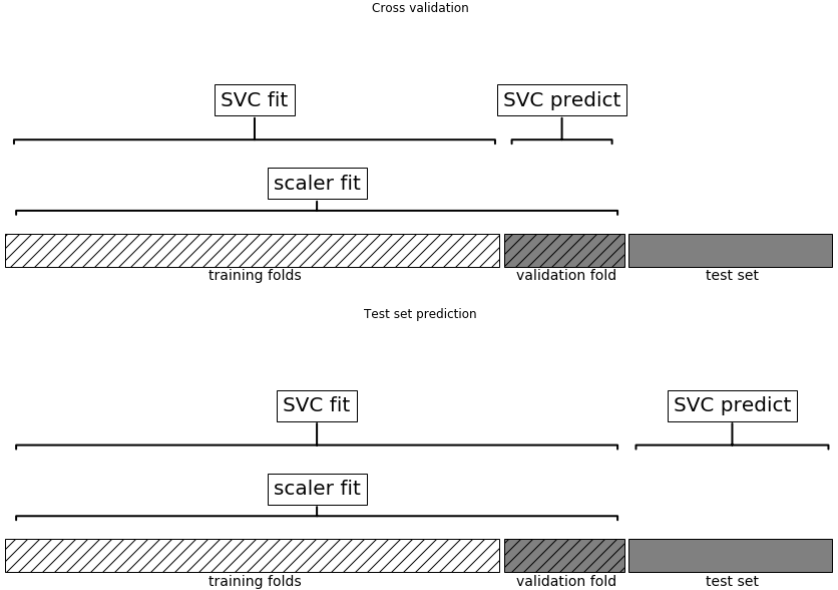
\includegraphics[scale=0.55]{Imagen_Machine/Pipe1.png}
      \caption{Uso de datos al preprocesar fuera del ciclo (Bucle) de validación cruzada}
      \label{Pipe1}
   \end{figure}
   
   
   Por lo tanto, las divisiones en la validación cruzada ya no reflejan correctamente cómo 
   se verán los nuevos datos en el proceso de modelado. Ya filtramos información de estas partes de la data en el proceso de modelado.  Esto conducirá a resultados demasiado optimistas durante
   validación cruzada, y posiblemente la selección de parámetros subóptimos.\\
   
   
   Para evitar este problema, la división del conjunto de datos durante la validación cruzada debe hacerse antes de hacer cualquier preprocesamiento. Cualquier proceso que extraiga conocimiento del conjunto de datos sólo debe aplicarse a la parte de la data de entrenamiento, por lo que cualquier validación cruzada debe ser el fuera del "{}bucle"{} en su procesamiento.\\

   En {\ttfamily scikit-learn} se lograr esto  con las funciones {\ttfamily cross\_val\_score} y    {\ttfamily Grid SearchCV}, mediante el uso de la clase {\ttfamily  Pipeline}. La clase {\ttfamily  Pipeline} es una clase que permite "{}pegar"{}  múltiples pasos de procesamiento en un sólo estimador de {\ttfamily scikit-learn}.
   La clase Pipeline tiene métodos de ajuste, predicción y métodos de  puntuación,  y se comporta como cualquier otro modelo en {\ttfamily scikit-learn}. El caso de uso más común de la clase {\ttfamily  Pipeline} es encadenar pasos de preprocesamiento (como escalar los datos) junto con un modelo supervisado como un clasificador.
   

   
   \subsection{Construyendo  Pipelines}
   
   Veamos cómo podemos usar la clase {\ttfamily  Pipeline} para expresar el flujo de trabajo para entrenar un modelo SVM después de escalar los datos con {\ttfamily MinMaxScaler} (por ahora sin  grid search). Primero, construimos un objeto  {\ttfamily  Pipeline} proporcionándole una lista de pasos. Cada paso es una tupla que contiene un nombre (cualquier cadena de su elección\footnote{Con una excepción: el nombre no puede contener un doble guión bajo, \_\_.}) y una instancia de un estimador:
   
   
\begin{lstlisting}%[frame=single]
   
In[5]:
   
   from sklearn.pipeline import Pipeline
   pipe = Pipeline([("scaler", MinMaxScaler()), ("svm", SVC())])
   
\end{lstlisting}
   

   Aquí, creamos dos pasos: el primero paso es el  llamado  de  "{}scaler"{}, es una instancia de {\ttfamily  MinMaxScaler}, y el segundo es  el llamado del modelo  "{}svm"{}, es una instancia de SVC. Ahora, podemos ajustar la {\ttfamily  Pipeline}, como cualquier otro estimador {\ttfamily scikit-learn}:
   
   \begin{lstlisting}%[frame=single]
      
In[6]:
   
   pipe.fit(X_train, y_train)   
   \end{lstlisting}  
   
   Aquí {\ttfamily pipe.fit},  el primer paso se llama el {\ttfamily fit} y hace el escalado de la data,  transforma la data de entrenamiento usando la escala definida, y finalmente se ajusta el modelo  SVM con la data escalada. Para evaluar sobre la data de prueba, simplemente llamamos a {\ttfamily pipe.score}:
   
   
   \begin{lstlisting}%[frame=single]
   
In[7]:
   
   print("Test score: {:.2f}".format(pipe.score(X_test, y_test)))
   
Out[7]:
   
   Test score: 0.95      
   \end{lstlisting}
   
   
   Llamando al método de puntuación sobre   pipeline,  primero transforma los datos de prueba usando la
   escala, y luego llama al método de puntuación sobre  el SVM usando la data de prueba escalada.
   Como  puede ver, el resultado es idéntico al que obtuvimos con el código al comienzo del
   capítulo, al hacer las transformaciones a mano.   Usando   pipeline, reducimos el
   código necesario para el proceso de "{}preprocesamiento {\scriptsize +}clasificación"{}. 
   Sin embargo, el principal beneficio de  usar  pipeline,  es que ahora podemos usar este estimador único en
   {\ttfamily cross\_val\_score} o   {\ttfamily GridSearchCV}.
   
   
   
   
   \subsection{Usando Pipelines en búsquedas de cuadrícula \\(Grid Searches)}
   
   Usando una pipeline con una búsqueda de cuadrícula  (grid search) funciona de la misma manera que usar cualquier otro estimador. Se define una la cuadrícula de parámetros,   y se construye un {\ttfamily GridSearchCV}  desde  la pipeline y la cuadrícula de parámetros. 
   
   Al especificar  la cuadrícula de parámetros, hay un ligero cambio; sin embargo,  necesitamos especificar para cada parámetro a qué paso del pipeline pertenece.   Ambos parámetros que queremos ajustar, {\ttfamily C  } y  {\ttfamily gamma}, son parámetros de SVC, el segundo paso. Le dimos a este paso el nombre  {\ttfamily  "{}svm"{}.}
   
   
   La sintaxis para definir una cuadrícula de parámetros en una pipeline  es para especificar por  cada parámetro el nombre del paso, seguido por un {\bf  \_\!\_} (un doble guión bajo), y  nombre del parámetro seguido.   De esta forma para buscar sobre el parámetro C  de SVC, tenemos que usar  {\ttfamily "{}svm{\bf \_\!\_}C"{} } como clave en el diccionario de cuadrícula de parámetros, y de manera similar para {\ttfamily gamma}:   
   
   \begin{lstlisting}   
   
In[8]:
   
   param_grid = {'svm__C': [0.001, 0.01, 0.1, 1, 10, 100],
                 'svm__gamma': [0.001, 0.01, 0.1, 1, 10, 100]} 
   \end{lstlisting}
   
   Con esta cuadrícula de parámetros podemos usar {\ttfamily GridSearchCV} como de costumbre:
     
        
   \begin{lstlisting}   
   
In[9]:
   
   grid = GridSearchCV(pipe, param_grid=param_grid, cv=5)
   grid.fit(X_train, y_train)
   print("Best cross-validation accuracy: {:.2f}".format(grid.best_score_))
   print("Test set score: {:.2f}".format(grid.score(X_test, y_test)))
   print("Best parameters: {}".format(grid.best_params_))
   
Out[9]:
   
   Best cross-validation accuracy: 0.98
   Test set score: 0.97
   Best parameters: {'svm__C': 1, 'svm__gamma': 1}   
   \end{lstlisting}
   
   En contraste con la búsqueda de cuadrícula que hicimos antes, ahora por  cada división en la validación cruzada, el {\ttfamily MinMaxScaler} es reacondicionado reajustado con sólo las divisiones del entrenamiento y no se filtra información de la división de prueba en la búsqueda de parámetros. 
   
   Esto se compara  (Figura \ref{Pipe2}) con la Figura {Pipe1} anterior en este capítulo:   
   
   \begin{lstlisting}
   
In[10]:
   
   mglearn.plots.plot_proper_processing()
   
   \end{lstlisting}
   
   \begin{figure}[h!]
      \centering
      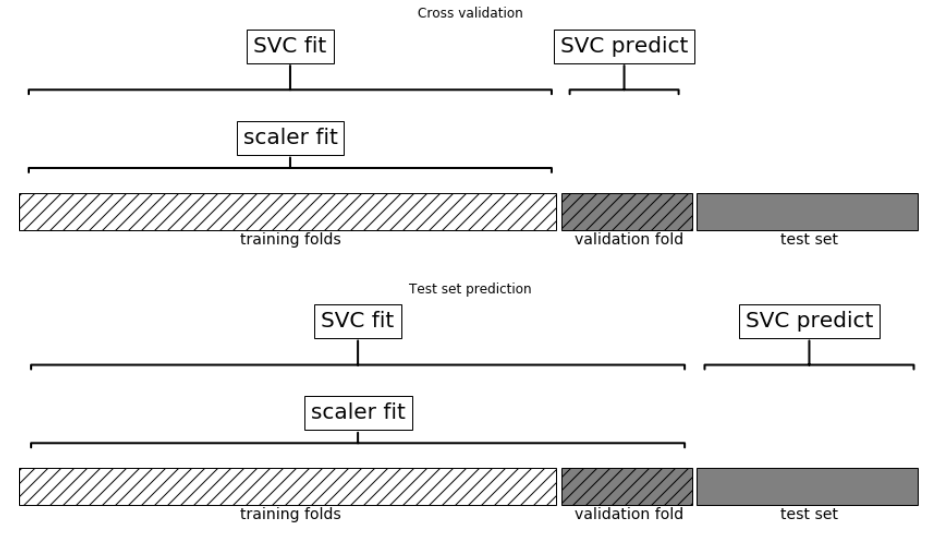
\includegraphics[scale=0.55]{Imagen_Machine/Pipe2}
      \caption{Uso de datos al preprocesamiento dentro del bucle de validación cruzada con una pipeline}
      \label{Pipe2}
   \end{figure}
   
     
   El impacto del filtrado de la información en la validación cruzada varía dependiendo de la naturaleza del paso de preprocesamiento. Estimar la escala de los datos usando el fold  de prueba por lo general no tiene un impacto terrible, mientras que el usando el fold de prueba en la extracción de características y la selección de características puede conducir a diferencias sustanciales en los resultados.
   
   
   
   
   
   
   %%%%%%%%%%%%%%%%%%%%%%%%%%%%%%%%    Caja     %%%%%%%%%%%%%%%%%%%%%%%%%%%%%%%%%%%%%%%%%
   
   
   
   
   
   
   
   \begin{longtable}{|p{13.25cm}|}  
      
      
      \arrayrulecolor{red}\hline
      
      \begin{center}
         {\bf{Ilustrando la filtración de información}}
      \end{center}
      
      \endfirsthead
      %   \hline
      
      Un gran ejemplo de información filtrada en validación cruzada se da en  el libro  The Elements of Statistical Learning  de  Friedman’s  de  Hastie,   Tibshirani,  aquí reproducimos una versión adaptada.    Consideremos una tarea de regresión sintética con 100 muestras y 10.000 características
		que se muestrean independientemente de una distribución gaussiana. También se muestrea
		la respuesta de una distribución gaussiana:       \\
		
		%	\endhead
		
		{ \ttfamily   
			{\scriptsize{  	
					
	            In[11]:
               \vspace{0.1cm}
               
     
   
            {\color{blue}   {\textbf
          {\hspace{0.6cm}from  rnd = np.random.RandomState(seed={\color{red} 0})}
                     
           \hspace{0.6cm}X = rnd.normal(size=({\color{red}  100 }, {\color{red}  10000})    \vspace{-0.2cm} 
                     
           \hspace{0.6cm}y = rnd.normal(size=({\color{red} 100},))  
      }  }}}}\\       
      
      \vspace{-0.251cm}
      
      
      Dada la forma en que creamos la dataset, no hay relación entre los datos   X,  y  el
      objetivo $y$ (target)  (es decir, son independientes), por lo que no debería ser posible aprender nada de  esta  dataset. Ahora haremos lo siguiente. Primero, seleccionemos las  características  más informativas de los 10,   usando para la selección de características {\ttfamily SelectPercentile}, y
   	luego evaluamos al regresor Ridge   utilizando validación cruzada: \\  
		
		
		{ \ttfamily   
			{\scriptsize{  	
					
					In[12]:
					\vspace{0.1cm}
					
				\hspace{0.6cm}{\color{blue} {\textbf   from  sklearn.feature\_selection import SelectPercentile, f\_regression
							
				\hspace{0.6cm}select = SelectPercentile(score\_func=f\_regression, percentile=  {\color{red} 5}).fit(X, y)
							
				\hspace{0.6cm}X\_selected = select.transform(X)  
							
				\hspace{0.6cm}print({\color{red}  "{}X\_selected.shape: "{}}.format(X\_selected.shape))   }}
					\vspace{0.1cm}
					
					Out[12]:
					\vspace{0.1cm}
					
					\hspace{0.6cm}X\_selected.shape: (100, 500)
					\vspace{0.1cm}
					
					In[13]:
					\vspace{0.1cm}
					
				\hspace{0.6cm}{\color{blue}	{\textbf from  sklearn.model\_selection import cross\_val\_score
							
				\hspace{0.6cm}from sklearn.linear\_model import Ridge
							
				\hspace{0.6cm}print({\color{red}  "{}Cross-validation accuracy (cv only on ridge): {:.2f}"{}}.format(
							
				\hspace{1.65cm}np.mean(cross\_val\_score(Ridge(), X\_selected, y, cv={\color{red} 5}))))
					}}
					\vspace{0.1cm}
					
					Out[13]:
					\vspace{0.1cm}
					
			\hspace{0.6cm}Cross-validation accuracy (cv only on ridge): 0.91 }}}	\\
		
		\vspace{-0.251cm}
		
		
		La promedio  de  $R^{2}$  calculada  por validación cruzada es  0.91,  lo que indica un modelo muy bueno. 
		Esto claramente no puede ser correcto, ya que los datos son completamente aleatorios. 
		Lo que sucedió aquí es que nuestra selección de características escogió algunas características
		entre las 10.000 características aleatorias que están (por casualidad) muy bien correlacionadas
		con el objetivo. Debido a que ajustamos la selección de características fuera de la 
		validación cruzada, podría 		encontrar características que están correlacionadas tanto en el entrenamiento como en los folds  		 de prueba. 
		La información que filtramos de los folds  de prueba fue muy informativa, lo que 
		llevó a resultados muy poco realistas. Comparemos esto con una validación cruzada apropiada
		usando una pipeline:\\
		
		
		{ \ttfamily   
			{\scriptsize{  	
					
					In[14]:
					\vspace{0.1cm}
					
				\hspace{0.6cm}{\color{blue} {\textbf   pipe = Pipeline([("{}select"{}, SelectPercentile(score\_func=f\_regression,
							
			\hspace{3.4cm}percentile=5)), ("{}ridge"{}, Ridge())])
							
			\hspace{0.6cm}print("{}Cross-validation accuracy (pipeline): {:.2f}"{}.format(
							
			\hspace{1.65cm}np.mean(cross\_val\_score(pipe, X, y, cv=5))))  } }
					\vspace{0.1cm}
					
					Out[14]:
					\vspace{0.1cm}
					
			\hspace{0.6cm}Cross-validation accuracy (pipeline): -0.25  }}}	\\
		
		\vspace{-0.251cm}
		
		
		Esta vez, obtenemos una puntuación $R^{2}$  negativa, indicando un modelo muy pobre.
		Utilizando la pipeline, la selección de características se encuentra ahora dentro del bucle 
		de validación cruzada. Esto significa que las características sólo se pueden seleccionar 
		utilizando los folds  de la data de entrenamiento, no el folds de prueba. 
		La selección de características encuentra las características que están correlacionadas
		con el objetivo en el conjunto de entrenamiento, pero debido a que los datos son 
		completamente aleatorios, estas características no están correlacionadas con el objetivo 
		en el conjunto de pruebas. En este ejemplo, rectificar el problema de la filtración de la 
		data en la selección  característica hace la diferencia entre la conclusión de que un modelo
		funciona muy bien y la conclusión de que un modelo no funciona en absoluto. \\
		% \vspace{0.1cm}
		\\  	
		\arrayrulecolor{red}\hline
		
	\end{longtable}
	

	
	\section{Interfaz general  de  Pipeline}
	
	La clase Pipeline no está restringida al preprocesamiento y clasificación, sino que puede
	unir cualquier cantidad de estimadores. Por ejemplo, podría construir una  pipeline
	que contiene la extracción de características, selección de características, escalado y clasificación, para un total de cuatro pasos. Del mismo modo, el último paso podría ser la regresión o clúster en lugar de la clasificación.  El único requisito para los estimadores en una pipeline es que todos, excepto el último paso, necesitan tener un método de transformación, para que puedan producir una nueva representación de los datos que se puede usar en el siguiente paso.\\
	
	
	Internamente, durante el  llamado a {\ttfamily Pipeline.fit},  pipeline llama {\ttfamily fit }  y luego   {\ttfamily  transform}  en cada paso por turno\footnote{O simplemente {\ttfamily fit\_transform}}, con la entrada dada por la salida del método de {\ttfamily  transform} del paso anterior. 
	Para el último paso en pipeline, sólo se llama {\ttfamily fit}.\\
	
	
	%    Brushing   raspando   Repasando algunos detalles más finos,
	%    Brushing over some finer details, this is implemented as follows. %
	
	Al dejar algunos detalles más finos, esto se implementa de la siguiente manera.
	Recuerda que {\ttfamily pipeline.steps} es una lista de tuplas, por lo que {\ttfamily pipeline.steps[0][1] }  es el primer estimador, {\ttfamily pipeline.steps[1][1]} es el segundo estimador, y así sucesivamente:
	
	
	\begin{lstlisting}%[frame=single]
	
In[15]:
   
   def fit(self, X, y):
       X_transformed = X
       for name, estimator in self.steps[:-1]:
           # iterate over all but the final step
           # fit and transform the data
           X_transformed = estimator.fit_transform(X_transformed, y)
       # fit the last step
       self.steps[-1][1].fit(X_transformed, y)
       return self   
   \end{lstlisting}
   

   Al predecir usando  {\ttfamily Pipeline}, transformamos de manera similar los datos con  {\ttfamily transform},   usando todo menos el último paso, y luego llamamos a predecir con  {\ttfamily predict} en el último paso:
   
   \begin{lstlisting}%[frame=single]
   
In[16]:
   
   def predict(self, X):
       X_transformed = X   
       for step in self.steps[:-1]:
           # iterate over all but the final step
           # transform the data
           X_transformed = step[1].transform(X_transformed)
       # fit the last step
       return self.steps[-1][1].predict(X_transformed)	
	\end{lstlisting}
	
	
	
	El proceso se ilustra en la figura \ref{Pipe3} para dos transformadores, T1,  T2, y un clasificador (llamado  {\ttfamily Classifier} ).
	
	\begin{figure}[h!]
		\centering
		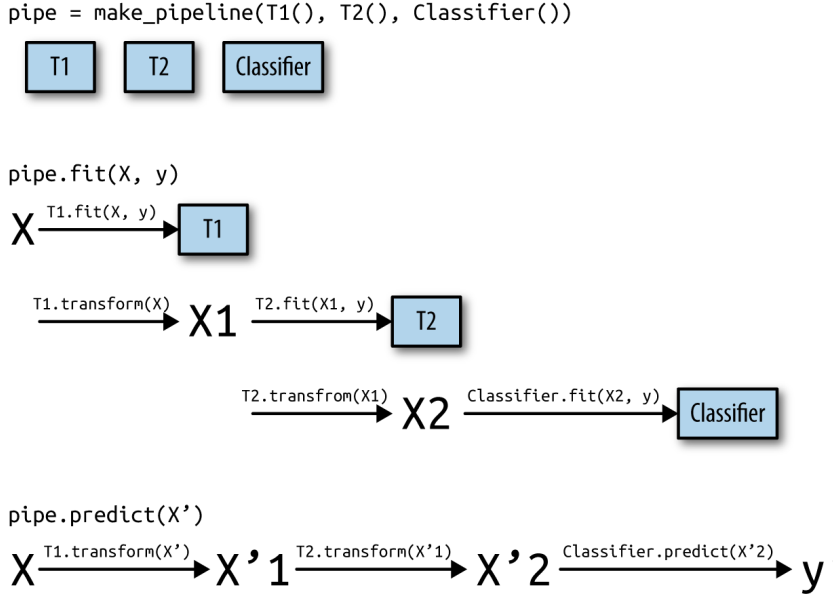
\includegraphics[scale=0.65]{Imagen_Machine/Pipe3}
		\caption{Descripción general del proceso de entrenamiento y predicción de pipeline}
		\label{Pipe3}
	\end{figure}
	
	
	La pipeline es incluso más general que esto. No es necesario que el último paso en un pipeline para 
	tener  una función de predicción, y podríamos crear una pipeline que sólo contenga, por ejemplo, un escalador y un PCA. Entonces, debido a que el último paso (PCA) tiene un método de transformación, podríamos llamar a {\ttfamily transform} en la pipeline  para obtener la salida de {\ttfamily  PCA.transform} aplicada a los datos que se procesaron en el paso anterior. El último paso de una pipeline sólo se requiere  tener un método {\ttfamily fit}.
	
	\newpage
	
	\subsection{Creando  una  Pipeline   con  {\ttfamily make\_pipeline}}

     	%  cumbersome  =    engorroso
	
	Crear una pipeline  usando la sintaxis descrita anteriormente es algunas veces un poco engorroso, y a menudo no necesitamos usar nombres especificos por cada paso. Hay una función de conveniencia, {\ttfamily make\_pipeline}, que creará una pipeline personal y nombrará automáticamente cada paso basado en su clase. La sintaxis para {\ttfamily make\_pipeline}, es la siguiente:
	
	
	
	\begin{lstlisting}%[frame=single]
	
In[17]:
	
   from sklearn.pipeline import make_pipeline
   # standard syntax
   pipe_long = Pipeline([("scaler", MinMaxScaler()), ("svm", SVC(C=100))])
   # abbreviated syntax
   pipe_short = make_pipeline(MinMaxScaler(), SVC(C=100))   
   \end{lstlisting}
   
   
   Los objetos pipeline son {\ttfamily pipe\_long}  y  {\ttfamily pipe\_short}  hacen exactamente lo mismo, pero {\ttfamily pipe\_short} tiene pasos que se nombran automáticamente. Podemos ver los nombres de los pasos observando el atributo {\ttfamily steps}:
   
   
   \begin{lstlisting}%[frame=single]
   
   
In[18]:
   
   print("Pipeline steps:\n{}".format(pipe_short.steps))
   
Out[18]:
   
   Pipeline steps:
   [('minmaxscaler', MinMaxScaler(copy=True, feature_range=(0, 1))),
    ('svc', SVC(C=100, cache_size=200, class_weight=None, coef0=0.0,
                decision_function_shape=None, degree=3, gamma='auto',
                kernel='rbf', max_iter=-1, probability=False,
                random_state=None, shrinking=True, tol=0.001,
                verbose=False))]   
   \end{lstlisting}
   
   	
	Los pasos se llaman {\ttfamily minmaxscaler}  y  {\ttfamily svc}. En general, los nombres de los pasos 
	son sólo versiones minúsculas de los nombres de clase. Si varios pasos tienen la misma clase,
	se añade un número:
	
	\begin{lstlisting}%[frame=single]
   
In[19]:
   
   from sklearn.preprocessing import StandardScaler
   from sklearn.decomposition import PCA
   
   pipe = make_pipeline(StandardScaler(), PCA(n_components=2), 
                        StandardScaler())
   print("Pipeline steps:\n{}".format(pipe.steps))
   
Out[19]:
   
   Pipeline steps:
   [('standardscaler-1', StandardScaler(copy=True, with_mean=True,
                                        with_std=True)), 
    ('pca', PCA(copy=True, iterated_power=4, n_components=2, 
                random_state=None, svd_solver='auto', tol=0.0,
                whiten=False)), 
    ('standardscaler-2', StandardScaler(copy=True, with_mean=True, 
                                         with_std=True))]   
   \end{lstlisting}
  	
	Como puedes ver, el primer paso {\ttfamily StandardScaler} fue nombrado como  {\ttfamily standardscaler-1} y el segundo paso lo nombra como {\ttfamily standardscaler-1}. Sin embargo, en tales escenarios podría ser mejor usar la construcción del {\ttfamily Pipeline} con nombres explícitos, para dar nombres relacionados con cada paso.
	
	\subsection{Acceso a los atributos por pasos}
	
	
	Es posible que se necesite inspeccionar los atributos en uno de los pasos de la pipeline, por ejemplo, los coeficientes de un modelo lineal o los componentes extraídos por PCA. La forma más fácil de acceder a los pasos en una pipeline es a través del atributo {\ttfamily named\_steps}, que es un diccionario de los nombres de los pasos en los estimadores:	
	
	
	\begin{lstlisting}%[frame=single]
	
In[20]:
	
   # fit the pipeline defined before to the cancer dataset
   pipe.fit(cancer.data)
   # extract the first two principal components from the "pca" step
   components = pipe.named_steps["pca"].components_
   print("components.shape: {}".format(components.shape))
   
Out[20]:
   
    components.shape: (2, 30)   
	\end{lstlisting}
	
	
	
	\subsection{Acceso a atributos de una Pipeline dentro de una  buscada de cuadrícula}
	%   Grid-Searched 
	
	
	
	Como discutimos anteriormente en este capítulo, una de las principales razones para usar las
	pipelines  es para hacer búsquedas de cuadriculas (grid searches). Una tarea común es acceder 
	 a algunos de los pasos   de una pipelines dentro de una búsqueda  cuadrícula.
	Hagamos una Busqueda de cuadrícula en el clasificador   {\ttfamily LogisticRegression} sobre la dataset de cáncer, usando {\ttfamily Pipeline} y {\ttfamily StandardScaler} para 
	escalar los datos antes de pasarlos al clasificador  {\ttfamily LogisticRegression}.  Primero creamos una pipeline usando la función {\ttfamily make\_pipeline}: 
	
	
	\begin{lstlisting}%[frame=single]
	
In[21]:
	
   from sklearn.linear_model import LogisticRegression
   
   pipe = make_pipeline(StandardScaler(), LogisticRegression())   
   \end{lstlisting} 
	
	
	A continuación, creamos una cuadrícula de parámetros. Como se explicó en el capítulo \ref{Cap2}, 
	\: el parámetro de regularizaciónen  para ajustar en  {\ttfamily LogisticRegression}, es el parámetro C. Usamos una cuadrícula logarítmica para este parámetro, buscando entre 0.01 y 100. Debido a que usamos la función {\ttfamily make\_pipeline}, el nombre del paso {\ttfamily LogisticRegression } en la pipeline  es el nombre de clase en letras minúsculas, {\ttfamily logisticregression}.   Por lo tanto para ajustar el parámetro C, tenemos que especificar una cuadrícula de parámetros para {\ttfamily logisticregression{\scriptsize\_\!\_\!\_}C}:
	
	\begin{lstlisting}
	
In[22]:
	
   param_grid = {'logisticregression__C': [0.01, 0.1, 1, 10, 100]}
   
   \end{lstlisting}
   
   
   Como de costumbre, dividimos la dataset del cáncer en dos conjuntos, el de entrenamiento y el prueba, y ajustamos una búsqueda de cuadrícula:   
   
   \begin{lstlisting}
   
In[23]:
   
   X_train, X_test, y_train, y_test = train_test_split(
       cancer.data, cancer.target, random_state=4)
   grid = GridSearchCV(pipe, param_grid, cv=5)
   grid.fit(X_train, y_train)
   
   \end{lstlisting}
   
   Y ahora, ¿cómo accedemos a los coeficientes del mejor modelo de  clasificación {\ttfamily LogisticRegression}    encontrado por {\ttfamily  GridSearchCV} ?.    Del Capítulo \ref{Cap5} sabemos que el     mejor  modelo encontrado por  {\ttfamily  GridSearchCV}, entrenado en todos los datos de entrenamiento, es almacenado en {\ttfamily grid.best\_estimator\_}:
   
   
   \begin{lstlisting}%[frame=single]
   
In[24]:
   
   print("Best estimator:\n{}".format(grid.best_estimator_))
	
Out[24]:
   
   Best estimator:
   Pipeline(steps=[
       ('standardscaler', StandardScaler(copy=True, with_mean=True, 
         with_std=True)),
       ('logisticregression', LogisticRegression(C=0.1, class_weight=None,
         dual=False, fit_intercept=True, intercept_scaling=1, max_iter=100,
         multi_class='ovr', n_jobs=1, penalty='l2', random_state=None,
         solver='liblinear', tol=0.0001, verbose=0, warm_start=False))])   
   \end{lstlisting}
   En este caso se accede a los pasos con  {\ttfamily best\_estimator\_}. Ahora, en nuestro caso que es una pipeline con dos pasos, {\ttfamily
      standardscaler}  y  {\ttfamily logisticregression}, para acceder a los pasos  se  usar el atributo {\ttfamily  named\_steps} de la pipeline,   en   {\ttfamily logisticregression},  como se explicó anteriormente.
   
   \begin{lstlisting}%[frame=single]
   
In[25]:
   
   print("Logistic regression step:\n{}".format(
          grid.best_estimator_.named_steps["logisticregression"]))
   
Out[25]:
	
   Logistic regression step:
   LogisticRegression(C=0.1, class_weight=None, dual=False, 
                      fit_intercept=True, intercept_scaling=1,
                      max_iter=100, multi_class='ovr', n_jobs=1,
                      penalty='l2', random_state=None, 
                      solver='liblinear', tol=0.0001, verbose=0,
                      warm_start=False)
   
   \end{lstlisting}
   
	Ahora que hemos entrenado la instancia  {\ttfamily LogisticRegression}, podemos acceder a los coefficientes (o pesos) asociados con cada característica de entrada:	
	
	
	\begin{lstlisting}%[frame=single]
	
In[26]:
	
   print("Logistic regression coefficients:\n{}".format(
          grid.best_estimator_.named_steps["logisticregression"].coef_))
   
Out[26]:
   
   Logistic regression coefficients:
   [[-0.389 -0.375 -0.376 -0.396 -0.115 0.017 -0.355 -0.39 -0.058 0.209
   -0.495 -0.004 -0.371 -0.383 -0.045 0.198 0.004 -0.049 0.21 0.224
   -0.547 -0.525 -0.499 -0.515 -0.393 -0.123 -0.388 -0.417 -0.325 -0.139]]   
   \end{lstlisting}
   
   Esto puede ser una expresión algo larga, pero con frecuencia es útil  para entender los modelos.
   
   \subsection{Pasos en el preprocesamiento de búsqueda de cuadrícula y parámetros del modelo} 
	% Grid-Searching Preprocessing Steps and Model Parameters 
	
	Usando pipelines, podemos encapsular todos los pasos de procesamiento en el flujo de trabajo del aprendizaje automático en un sólo estimador de {\ttfamily  scikit-learn}.  	Otro beneficio de usar el pipelina, es que ahora podemos ajustar los parámetros del 
	preprocesamiento utilizando  el resultado de una tarea supervisada como la regresión
	o clasificación.
	
	En capítulos anteriores, utilizamos  algunas  características polinómicas en la dataset  boston antes de aplicar el regresor ridge. Ahora vamos a modelar esto  utilizando una pipeline. La pipeline contiene tres pasos:  escala la data,  cálculo las características polinómicas, y la regresión de ridge:
	
	
	
	\begin{lstlisting}%[frame=single]
	
In[27]:
	
   from sklearn.datasets import load_boston
   boston = load_boston()
   X_train, X_test, y_train, y_test = train_test_split(
        boston.data, boston.target, random_state=0)
   
   from sklearn.preprocessing import PolynomialFeatures
   pipe = make_pipeline( StandardScaler(),
                         PolynomialFeatures(),
                         Ridge())
   
   \end{lstlisting}
   
   
   
   ¿Cómo sabemos qué grados de polinomios elegir, o qué  polinomio   elegir o qué interacciones? Idealmente queremos seleccionar el parámetro de grado basado en el resultado de la clasificación.
	Usando nuestra   pipeline, podemos buscar sobre el parámetro  {\ttfamily degree} junto con el parámetro {\ttfamily alfa} de {\ttfamily  Ridge}. Para hacer esto, definimos el parámetro  {\ttfamily param\_grid} que contiene ambos, adecuadamente prefijado por los nombres del respectivo  paso: 
	
	
	\begin{lstlisting}%[frame=single]
	
In[28]:
	
    param_grid = {'polynomialfeatures__degree': [1, 2, 3],
                  'ridge__alpha': [0.001, 0.01, 0.1, 1, 10, 100]}   
   \end{lstlisting}
   
	
	
	
	Ahora podemos correr nuevamente la busqueda de cuadrícula:
	
	
	\begin{lstlisting}%[frame=single]
	
	
In[29]:
	
   grid = GridSearchCV(pipe, param_grid=param_grid, cv=5, n_jobs=-1)
   grid.fit(X_train, y_train)	
	\end{lstlisting}	
	
	
Podemos visualizar el resultado de la validación cruzada usando un mapa caliente  (Figura \ref{Pipe4}), como hicimos en el Capítulo \ref{Cap5}:
	
	
	\begin{lstlisting}%[frame=single]
	
In[30]:
	
   plt.matshow(grid.cv_results_['mean_test_score'].reshape(3, -1),
               vmin=0, cmap="viridis")
   plt.xlabel("ridge__alpha")
   plt.ylabel("polynomialfeatures__degree")
   plt.xticks(range(len(param_grid['ridge__alpha'])), 
              param_grid['ridge__alpha'])
   plt.yticks(range(len(param_grid['polynomialfeatures__degree'])),
              param_grid['polynomialfeatures__degree'])
   
   plt.colorbar()	
	\end{lstlisting}	

	
	\begin{figure}[h!]
		\centering
		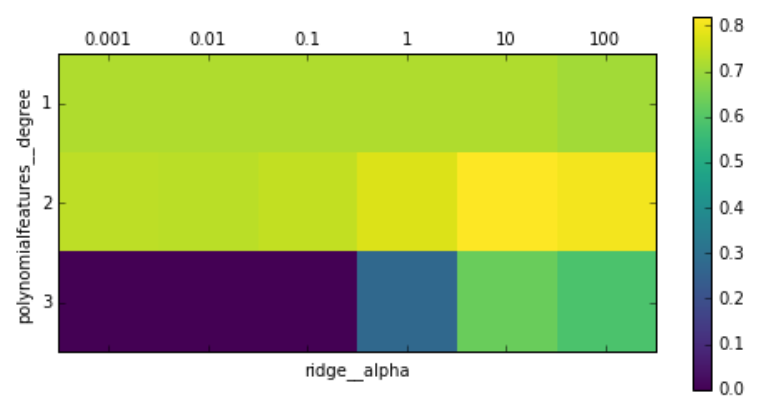
\includegraphics[scale=0.55]{Imagen_Machine/Pipe4}
		\caption{Mapa caliente del puntuación media de la validación cruzada como  función del grado de las características polinómicas y del parámetro {\ttfamily alfa} de  {\ttfamily  Ridge}}
		\label{Pipe4}
	\end{figure}
\newpage	
	Observando estos  resultados producidos por la validación cruzada, podemos ver que el uso 
	de polinomios de grado dos ayuda, pero que los polinomios de grado tres son mucho peores que cualquiera de los grados uno o dos. Esto se refleja en los mejores parámetros que se encontraron:
	
	
	\begin{lstlisting}%[frame=single]
	
In[31]:
	
   print("Best parameters: {}".format(grid.best_params_))
	
Out[31]:
	
   Best parameters: {'polynomialfeatures__degree': 2, 'ridge__alpha': 10}
	
	\end{lstlisting}
	
	Que conducen a la siguiente puntuación:
	
	
	
	\begin{lstlisting}%[frame=single]
	
In[32]:
	
   print("Test-set score: {:.2f}".format(grid.score(X_test, y_test)))
	
Out[32]:
	
   Test-set score: 0.77	
	\end{lstlisting}
	
	Vamos a ejecutar una búsqueda de cuadrícula sin características polinómicas para la comparación:
	
	
	
	\begin{lstlisting}%[frame=single]
	
In[33]:
	
   param_grid = {'ridge__alpha': [0.001, 0.01, 0.1, 1, 10, 100]}
   pipe = make_pipeline(StandardScaler(), Ridge())
   grid = GridSearchCV(pipe, param_grid, cv=5)
   grid.fit(X_train, y_train)
   print("Score without poly features: {:.2f}".format(
          grid.score(X_test, y_test)))
   
Out[33]:
   
	Score without poly features: 0.63
  \end{lstlisting}
 	
	
	Como se  esperaba, observando los resultados de búsqueda de cuadrícula visualizados en la figura \ref{Pipe4}, usando características no polinómicas conduce a resultados de puntajes más bajos, es decir, un modelo con rendimiento peor con respecto al anterior.\\
   %   ningún polinomio
	
	La búsqueda de parámetros de preprocesamiento junto con parámetros del modelo 
	es una estrategia muy poderosa. Sin embargo, tenga en cuenta que  {\ttfamily GridSearchCV }  
	intenta todas las combinaciones posibles de los parámetros especificados. Por lo tanto,
	agregar más parámetros a su cuadrícula aumenta exponencialmente el número de modelos que
	necesita construir.
	
	
	\subsubsection{Qué modelo utilizar y	Grid-Searching }
	
	%    Grid-Searching Which Model To Use

	
	Incluso puede ir más allá al combinar {\ttfamily GridSearchCV} y  {\ttfamily  Pipeline}: 
	también es posible  buscar  los pasos reales que se realizó la pipeline (ya sea usando {\ttfamily
		StandardScaler}  o   {\ttfamily MinMaxScaler}).
	Esto lleva a un espacio de búsqueda aún mayor y debe ser considerado cuidadosamente. Probar todas las soluciones posibles generalmente no es una estrategia viable de aprendizaje automático. 
	Sin embargo, aquí hay un ejemplo comparando un clasificador de {\ttfamily RandomForest}
	y uno de {\ttfamily  SVC} en la dataset Iris. Sabemos que el {\ttfamily  SVC} podría necesitar la dataset  escalar, por lo que también buscamos si se usa {\ttfamily  StandardScaler}  o no preprocesando.
	Para el {\ttfamily RandomForestClassifier}, sabemos que no es necesario ningún preprocesamiento.
	Comenzamos definiendo la pipeline; aquí, nombramos explícitamente los pasos. 
	Queremos dos pasos, uno para el preprocesamiento y el siguiente para un clasificador. Podemos instanciar esto 	usando {\ttfamily  SVC}  y  {\ttfamily  StandardScaler}:
		
	
	\begin{lstlisting}
	
In[34]:
   
   pipe = Pipeline([('preprocessing', StandardScaler()),
                    ('classifier', SVC())])   
   \end{lstlisting}
	
	%        “ busque sobre espacios que no son cuadrículas ”
	
	Ahora podemos definir el  {\ttfamily  parametr\_grid} para hacer la busqueda. Usaremos el clasificador  {\ttfamily RandomForestClassifier} o {\ttfamily SVC}. Ambos tienen diferentes parámetros para ajustar, por lo que  necesitan diferentes preprocesamientos, podemos hacer uso de la lista de  search grids  (búsqueda de cuadrículas)  que discutimos en "{}Buscar sobre espacios que no son cuadrículas"{}  en la página  \pageref{Pagina1}.
	
	
	Para asignarle  un estimador a un paso, usamos el nombre del paso como nombre del parámetro. Cuando necesitamos  saltar un paso en el pipeline (por ejemplo, porque no necesitamos preprocesamiento para {\ttfamily RandomForest}), no lo configuramos en ningún paso:	
	
	\begin{lstlisting}   
In[35]:
   
   from sklearn.ensemble import RandomForestClassifier
   
   param_grid = [
   {'classifier': [SVC()], 'preprocessing': [StandardScaler(), None],
   'classifier__gamma': [0.001, 0.01, 0.1, 1, 10, 100],
   'classifier__C': [0.001, 0.01, 0.1, 1, 10, 100]},
   {'classifier': [RandomForestClassifier(n_estimators=100)],
    'preprocessing': [None], 'classifier__max_features': [1, 2, 3]}]	
	\end{lstlisting}
	
Ahora podemos iniciar y ejecutar la búsqueda de cuadrícula como de costumbre, 
	en este caso sobre la data de cáncer:
	
	\begin{lstlisting}	
In[36]:
	
   X_train, X_test, y_train, y_test = train_test_split(
       cancer.data, cancer.target, random_state=0)
   
   grid = GridSearchCV(pipe, param_grid, cv=5)
   grid.fit(X_train, y_train)
   
   print("Best params:\n{}\n".format(grid.best_params_))
   print("Best cross-validation score: {:.2f}".format(grid.best_score_))
   print("Test-set score: {:.2f}".format(grid.score(X_test, y_test)))
	
Out[36]:
	
   Best params:
   {'classifier':
   SVC(C=10, cache_size=200, class_weight=None, coef0=0.0,
       decision_function_shape=None, degree=3, gamma=0.01, kernel='rbf',
       max_iter=-1, probability=False, random_state=None, shrinking=True,
       tol=0.001, verbose=False),
   'preprocessing':
   StandardScaler(copy=True, with_mean=True, with_std=True),
   'classifier__C': 10, 'classifier__gamma': 0.01}
   
   Best cross-validation score: 0.99
   Test-set score: 0.98	
	\end{lstlisting}
	
	
	El resultado de la búsqueda de cuadrícula es que {\ttfamily SVC} con preprocesamiento {\ttfamily StandardScaler}, {\ttfamily C=10}  y {\ttfamily  gamma=0.01} dio el mejor resultado.
	
	
	\section{Resumen y perspectivas}
	
	En este capítulo presentamos la clase {\ttfamily  Pipeline}, una herramienta de uso general para encadenar
	(unir) múltiples pasos de procesamiento en un flujo de trabajo del aprendizaje automático. 
	En aplicaciones del mundo real  del aprendizaje automático rara vez se usa un modelo  aislado, y generalmente son una secuencia de pasos de procesamiento.   	El uso de {\ttfamily  pipeline} nos permite encapsular múltiples pasos
	en un único objeto Python que se adhiere a la interfaz de {\ttfamily scikit-learn} con {\ttfamily fit,
	predict}, and {\ttfamily transform}.    En particular, cuando se realiza la evaluación del modelo mediante la validación cruzada y la selección de parámetros mediante la búsqueda de cuadrícula, utilizando la clase {\ttfamily  pipeline}  para capturar todos los pasos de procesamiento  es esencial para una evaluación adecuada.
	

	
	La clase Pipeline también permite escribir código más breve  y reduce la probabilidad de
	errores que pueden suceden al construir cadenas de procesamiento sin la clase pipeline (como olvidarse de aplicar todos las transformaciones en la data pruebas, o no aplicarlos en el orden correcto).
	Elegir la combinación correcta de extracción de características, preprocesamiento y modelos es
	algo así como un arte, y con frecuencia requiere algo de ensayo y error.
	Sin embargo, usando pipeline, esta "prueba" de muchos pasos de procesamiento diferentes es muy simple. 
	
	Al experimentar, tenga cuidado de no complicar demasiado sus procesos, y asegúrese de evaluar que  cada componente que está incluyendo   en su modelo  es necesario. \\  

	Con este capítulo, hemos completado nuestro estudio de herramientas de propósito general y algoritmos proporcionados por {\ttfamily scikit-learn}. Ahora posee todas las habilidades requeridas y conoce los mecanismos necesarios para aplicar el aprendizaje automático en la práctica. \\
	
	En el próximo capítulo, nos trataremos  con mayor detalle  un tipo particular de datos que 
	se ve comúnmente en la práctica, y que requiere algunos conocimientos especiales para manejar correctamente: datos de texto.
	
	
	
	
	
 
   

	
%\include{Portada3} 	

\chapter{Trabajando con Datos de Texto}\label{Cap7}


\section{Introducción}

En el Capítulo \ref{Cap4}, hablamos sobre dos tipos de características que pueden representar 
propiedades de la data: características continuas que describen una cantidad y características categóricas que son items  de una lista fija. Hay un tercer tipo de característica que se puede encontrar en muchos
aplicaciones,  el tipo  texto.  Por ejemplo, si queremos clasificar un mensaje de correo electrónico como
 un correo electrónico legítimo o spam, el contenido del correo electrónico ciertamente contendrá
información importante para esta tarea de clasificación.  O tal vez queremos aprender sobre la opinión de un político sobre el tema de la inmigración.  En este caso, los discursos o tweets de esta persona pueden proporcionar información útil.   En servicio al cliente, a menudo desea saber si un mensaje es una queja o una consulta.   Podemos usar la línea del tema y contenido de un mensaje para determinar automáticamente la intención del cliente, que nos permite enviar el mensaje al departamento correspondiente, o incluso enviar una  respuesta automática.\\


La data de texto generalmente  suelen representarse como cadenas (strings), compuestas de caracteres. En cualquiera de los ejemplos que se acaban de dar, la longitud de los datos de texto variará. Esta característica es claramente muy diferente de las características numéricas que hemos discutido hasta ahora, y tendremos que procesar los datos antes de que podamos aplicar nuestros algoritmos de aprendizaje automático sobre ellos.\\

% oraciones  críticas    reseñas o críticas comentarios 

\section{Tipos de datos representados como cadenas}

Antes de sumergirnos en los pasos de procesamiento que van en la representación de datos de texto para el aprendizaje automático, queremos discutir brevemente diferentes tipos de datos de texto que se  podría encontrar. El texto suele ser sólo una cadena en la dataset, pero no todas las características de cadena deben tratarse como texto. Una característica de cadena (string) algunas  veces puede representar variables categóricas, como discutimos en el Capítulo \ref{Cap5}. No hay manera de saber cómo tratar una característica de cadena antes de revisar la data.\\


\noindent Hay cuatro tipos de datos de cadena (string) que puede ver:

\begin{list}{$\bullet$}{}  
	
	\item Datos categóricos.
	
	\item  Cadenas libres que pueden asignarse semánticamente a categorías.
	
	\item   Datos de cadena estructurados.
	
	\item  Datos de texto. 
\end{list}Los datos categóricos son los datos  que viene en forma  de una lista fija. Digamos que recopila datos a través de una encuesta donde le preguntas a las personas su color favorito, con un menú desplegable que les permite  seleccionar entre "{}rojo"{}, "{}verde"{}, "{}azul"{}, "{}amarillo"{}, "{}negro"{}, "{}blanco"{}, "{}púrpura"{} y "{}rosa"{}. 
Esto dará como resultado una dataset con exactamente ocho posibles valores  diferentes, que claramente
codifican una variable categórica. Puede verificar  por  observación  si este es el caso de sus datos
(si ve muchas cadenas diferentes, es poco probable que esta sea una variable categórica) y confirmarlo calculando los valores únicos sobre el conjunto de datos, y posiblemente usando un histograma con  la frecuencia con que aparece cada uno. 
También es posible que desee verificar si cada variable corresponde realmente a una categoría que tiene sentido para su aplicación. Tal vez a la mitad de la existencia de su encuesta, alguien descubrió que
"{}negro"{} fue mal escrito como "{}negor"{} y posteriormente corrigió la encuesta. Como resultado, su
la data contiene "{}negor"{} y "{}negro"{}, que corresponden al mismo 
significado  semántico  y debe consolidarse.\\



Ahora imagine que en lugar de proporcionar un menú desplegable, proporciona un campo de texto para que los 
usuarios  proporcionen sus propios colores favoritos. Muchas personas pueden responder con el nombre de un un color, como "{}negro"{} o "{}azul"{}. Otros pueden cometer errores tipográficos, usar diferentes
ortografías como "{}gris"{} y "{}grises"{}, o use nombres más evocadores y específicos como "{}noche azul."{} También tendrás algunas entradas muy extrañas.  Algunos buenos ejemplos vienen
de la encuesta de color xkcd  (\href{https://blog.xkcd.com/2010/05/03/color-survey-results/}{\textcolor{vino}{xkcd Color Survey} }), donde la gente tuvo que nombrar colores y se les ocurrió nombres como "{}velociraptor cloaka"{}    y   "{}El consultorio  naranja de mi dentista.  Todavía recuerdo su  caspa lentamente flotando en mi enorme bostezo"{}; ejemplos como estos,  son difíciles de asignar a colores automáticamente (o en absoluto).   Las respuestas que puede obtener de un campo de texto pertenecen a la segunda categoría en la lista, son  \emph{cadenas libres que pueden asignarse semánticamente a categorías}. 
Estos datos probablemente sea mejor codificarlos  como una variable categórica, donde pueda 
seleccionar las categorías utilizando las entradas más comunes o definiendo categorías que capturen las respuestas de una manera que tenga sentido para su aplicación.  Se podría tener algunas categorías para colores estándar, tal vez una categoría  "{}multicolor"{}   para personas que dieron respuestas como  "{}rayas verdes y rojas"{}  y una   categoría  como  "{}otra"{}  para respuestas que no pueden ser codificadas de otra manera. 
 Este tipo de preprocesamiento de  cadenas pueden requerir mucho esfuerzo manual y no se automatizan fácilmente.  Si estás en una posición que  puede influir en la recopilación de datos, le recomendamos que evite valores introducidos de forma manual para conceptos que se capturan mejor utilizando variables categóricas.\\


Con frecuencia, los valores introducidos manualmente no corresponden a categorías fijas, pero todavía tienen alguna estructura subyacente, como direcciones, nombres de lugares o personas, fechas, números de teléfono o cualquier otro identificador. Este tipo de cadenas son a menudo muy difíciles de analizar, y su tratamiento es altamente dependiente del contexto y el dominio. Un tratamiento sistemático de estos casos está más allá del objetivo de este libro.\\


La categoría final de  datos de cadena son los datos de texto en forma libre (freeform) que consisten en frases o sentencias  (phrases or sentences). Los ejemplos incluyen tweets, registros de chat y reseñas de hoteles, así como las obras recopiladas de Shakespeare, el contenido de Wikipedia o la colección del Proyecto Gutenberg de 50.000 libros electrónicos.


 Todas estas colecciones contienen información principalmente como oraciones compuestas de palabras\footnote{Discutiblemente, el contenido de sitios Webes asociados a tweets contiene más información que el texto de tweets en sí mismos.}. Por simplicidad, asumamos que todos nuestros documentos están en un idioma, inglés\footnote{La mayor parte de lo que hablaremos en el resto del capítulo también se aplica a otros idiomas que usan el alfabeto romano, y parcialmente a otros idiomas con delimitadores de límites de palabras. El chino, por ejemplo, no  delimita los límites de las palabras y tiene otros desafíos que dificultan la aplicación de las técnicas de este capítulo.}. En el contexto del análisis de texto, el conjunto de datos a menudo se llama cuerpo (corpus), y cada punto de datos, representado como un sólo texto, se llama documento. Estos términos provienen de la comunidad de recuperación de información (IR) y procesamiento del lenguaje natural (PNL), ambos  se ocupan principalmente de datos de texto.

 
\subsection{Ejemplo de aplicación:  Análisis de Sentimiento a Comentarios de Película}
   
  
%   the information retrieval (IR) and natural language processing (NLP) community, \\
%    reviews comentarios reseñas\\

Como ejemplo en ejecución en este capítulo, usaremos una dataset de reseñas o comentarios de películas
 del sitio web de IMDb (Internet Movie Database) recopilados por el investigador de   Stanford Andrew Maas\footnote{La data está disponible en   
 \href{http://ai.stanford.edu/~amaas/data/sentiment/}{\color{vino} http://ai.stanford.edu/~amaas/data/sentiment/}.}.   Esta dataset  contiene el texto de los comentario, junto con una etiqueta que indica si un  comentario es "{}positivo"{}  o  "{}negativo."{}   El sitio web de IMDb contiene clasificaciones de 1 a 10. Para simplificar el modelado, esta anotación se resume como una  dataset de clasificación en dos clases, donde los comentarios con una puntuación igual o superior a 6 se etiquetan como positivos, y el resto como negativos. Se deja  la pregunta de si esta es una buena representación de los datos abiertos si mayor análisis, y simplemente usaremos la data según lo proporcionado por Andrew Maas.\\

Después de descomprimir los datos, se obtienen los archivos de texto  en dos carpetas separadas, una con los datos de entrenamiento y otra con los datos de prueba. Cada uno de estos a su vez tiene dos subcarpetas, una llamada  {\ttfamily pos} y otra llamada {\ttfamily neg} :

\begin{lstlisting}

In[2]:

   !tree -L 2 C:/Data/aclImdb_v1/aclImdb

Out[2]:

\end{lstlisting}
\vspace{-0.6cm}
\begin{figure}[h!]
	%\centering
	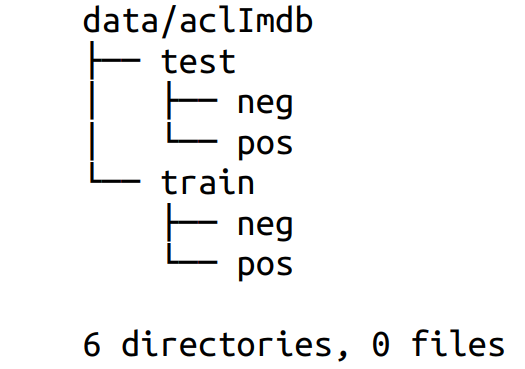
\includegraphics[scale=0.35]{Imagen_Machine/Texto1}
%	\caption{Matriz de confusión para clasificación binaria}
%	\label{Pipe3}
\end{figure}

La carpeta  {\ttfamily pos} contiene todas las críticas positivas, cada una como un archivo de texto separado, y similarmente  en  la carpeta  {\ttfamily neg}. 

Hay una función auxiliar en  {\ttfamily scikit-learn}  para cargar archivos almacenados con tal estructura de carpetas, donde cada subcarpeta corresponde a una etiqueta, llamada  {\ttfamily load\_files.} 
Aplicamos la función  {\ttfamily load\_files } primero a los datos de entrenamiento:
 
%   reviews_train = load_files("C:/A Cuadernos De Python/aclImdb_v1/aclImdb/train/")


\begin{lstlisting}

In[3]:

   # Descargue la data aqui:    (Archivo comprimido)
   #      http://ai.stanford.edu/~amaas/data/sentiment/aclImdb_v1.tar.gz
   
   # Mi direcccion es:   C:\Data\aclImdb_v1\aclImdb
   # Puede tardar 10 minutos o mas, paciencia
   
   from sklearn.datasets import load_files
   
   reviews_train = load_files("C:/Data/aclImdb_v1/aclImdb/train/")

  
   # load_files returns a bunch, containing training texts and 
   # training labels
   text_train, y_train = reviews_train.data, reviews_train.target
   print("type of text_train: {}".format(type(text_train)))
   print("length of text_train: {}".format(len(text_train)))
   print("text_train[1]:\n{}".format(text_train[1]))
  
Out[3]:

   type of text_train: <class 'list'>
   length of text_train: 25000
   text_train[1]:
   b'Words can\'t describe how bad this movie is. I can\'t explain it by
     writing only. You have too see it for yourself to get at grip of how 
     horrible a movie really can be. Not that I recommend you to do that. 
     There are so many clich\xc3\xa9s, mistakes (and all other negative 
     things you can imagine) here that will just make you cry. To start with 
     the technical first, there are a LOT of mistakes regarding the airplane.
     I won\'t list them here, but just mention the coloring of the plane. 
     They didn\'t even manage to show an  airliner in the colors of a 
     fictional airline, but instead used a 747 painted in the original 
     Boeing livery.  Very bad. The plot is stupid and has been done many 
     times before, only much, much better. There are so many ridiculous
     moments here that i lost count  of it really early. Also, I was on the
     bad guys\' side all the time in the movie, because the good guys were 
     so stupid. "Executive Decision" should without a doubt be you\'re choice
     over this one, even the "Turbulence"-movies are better. In fact, every
     other movie in the world is better than this one.'

\end{lstlisting}

% b'Las palabras no pueden describir lo mala que es esta película. No puedo explicarlo por escribiendo solamente. Tienes que verlo por ti mismo para saber cómo una película realmente horrible puede ser. No es que te recomiendo que hagas eso. Hay tantos clichés \ xc3 \ xa9s, errores (y todos los demás cosas que puedas imaginar) aquí que te harán llorar. Para empezar lo técnico primero, hay MUCHOS errores con respecto al avión.  No los enumeraré aquí, pero solo mencionaré el color del avión. Ni siquiera lograron mostrar un avión con los colores de un aerolínea ficticia, pero en su lugar usó un 747 pintado en el Boeing original  librea. Muy mal. La trama es estúpida y se ha hecho muchas veces antes,  solo que mucho, mucho mejor. Hay tantos momentos ridículos aquí que yo  Perdí la cuenta muy temprano. Además, estaba del lado de los malos todos el tiempo en la película, porque los buenos eran tan estúpidos. "Ejecutivo  La decisión "debe ser sin duda su elección sobre esta, incluso las películas de "Turbulencia" son mejores. De hecho, todas las demás películas del el mundo es mejor que este '.







Puedes ver que {\ttfamily text\_train} es una lista de longitud 25.000, donde cada entrada es una cadena que contiene una crítica o comentario. Imprimimos la reseña con el índice 1. También puede ver que la reseña contiene algunos saltos de línea HTML (<br />, breaks). Si bien es poco probable que estos tengan un gran impacto en nuestros modelos de aprendizaje automático, es mejor limpiar los datos y eliminar este formato antes de proceder:

\begin{lstlisting}%[frame=single]

In[4]:

   text_train = [doc.replace(b"<br />", b" ") for doc in text_train]

\end{lstlisting}


El tipo de  entrada de {\ttfamily text\_train} dependerá de la versión de Python. En Python 3, serán de tipo bytes  que representa una codificación binaria de los datos de cadena (strings). En Python 2, el {\ttfamily text\_train} contiene cadenas. Aquí, no entraremos en los detalles de los diferentes tipos de cadenas en Python, pero te recomendamos que leas la documentación de \href{https://docs.python.org/2/howto/unicode.html}{\textcolor{vino}{ Python 2} }  y/o  \href{https://docs.python.org/3/howto/unicode.html}{\textcolor{vino}{ de Python 3} } sobre cadenas y Unicode.\\

La dataset se recogió de tal manera que la clase positiva y la clase negativa sean balanceadas, de modo que hay tantas cadenas (string) positivas como negativas: 


\begin{lstlisting}%[frame=single]

In[5]:

   print("Samples per class (training): {}".format(np.bincount(y_train)))

Out[5]:
 
   Samples per class (training): [12500 12500] 
 \end{lstlisting}  
   
     Cargamos la dataset de prueba en la misma forma:
     
\begin{lstlisting}%[frame=single]

In[6]:

     
   reviews_test = load_files("C:Data/aclImdb_v1/aclImdb/test/") 
      
   text_test, y_test = reviews_test.data, reviews_test.target
   print("Number of documents in test data: {}".format(len(text_test)))
   print("Samples per class (test): {}".format(np.bincount(y_test)))
   text_test = [doc.replace(b"<br />", b" ") for doc in text_test]

Out[6]:

   Number of documents in test data: 25000
   Samples per class (test): [12500 12500]

\end{lstlisting}

La tarea que queremos resolver es la siguiente: dada una reseña o comentario, queremos 
asignarle una etiqueta  "{}positivo"{}  o  "{}negativo."{} basada en el contexto del comentario o 
reseña. Esta es una tarea de clasificación binaria estándar. Sin embargo, la data de texto
no está en formato para que el modelo de aprendizaje automatico pueda manejarlo.
Necesitamos convertir la representación de  cadenas (string) de texto  en representación 
numérica que pueda aplicarle el algoritmo de aprendizaje automático.

\subsection{Representando la data de texto en bolsas de palabras}

%  Representing Text Data as a Bag of Words}
%  palabras que no aportan información relevante sobre el texto. Ha estas palabras se les conoce como stopwords.
 
Una de las maneras más simples pero efectivas y comúnmente utilizadas para representar el texto para el aprendizaje automático es usando  la representación de la bolsa de palabras (del inglés, Bag of Words)\footnote{El modelo "bolsa de palabras" (del inglés, Bag of Words) es un método que se utiliza en el procesado del lenguaje para representar documentos ignorando el orden de las palabras. En este modelo, cada documento parece una bolsa que contiene algunas palabras. Por lo tanto, este método permite un modelado de las palabras basado en diccionarios, donde cada bolsa contiene unas cuantas palabras del diccionario.}. Al usar esta representación, descartamos la mayor parte de la estructura del texto de entrada, como capítulos, párrafos, oraciones y formatos, y sólo contamos {\emph{la frecuencia con la que cada palabra aparece en cada texto}}  del cuerpo.

 Descartando la estructura y contando sólo las ocurrencias de palabras conduce a la imagen mental de representar el texto como una "{}bolsa."{}  \\
 
  El cálculo de la representación de la bolsa de palabras para un cuerpo (corpus) de documentos consta de los tres pasos siguientes:
  
\begin{enumerate}
	
	\item \emph{Tokenización}. Dividir cada documento en las palabras que aparecen en él (llamadas tokens), por ejemplo, dividiéndolos en espacios en blanco y puntuación.
	
	\item \emph{La construcción de vocabulario}. Recoger un vocabulario de todas las palabras que aparecen en cualquiera de los documentos, y el número de ellos (por ejemplo, en orden alfabético). 
	
	\item \emph{Codificación}. Para cada documento, se cuenta la frecuencia   con   que  aparece cada palabras del vocabulario en este documento.
	
\end{enumerate}

Hay algunas sutilezas involucradas en los pasos 1 y 2, que discutiremos   más adelante con más detalle  en este capítulo. Por ahora, veamos cómo podemos aplicar el procesamiento de la bolsa de palabras usando {\ttfamily scikit-learn}. En la Figura \ref{Texto2} se ilustra el proceso en la cadena "{}Así es como se obtienen las hormigas{}". La salida es un vector de recuento de palabras para cada documento. 
Para cada palabra en el vocabulario, tenemos un recuento de la frecuencia con que aparece en cada documento. Eso significa que nuestra representación numérica tiene una característica para cada palabra única en toda la data. Observe cómo el orden de las palabras en la cadena original es completamente irrelevante para la representación de la función bag-of-words.

\begin{figure}[h!]
	\centering
	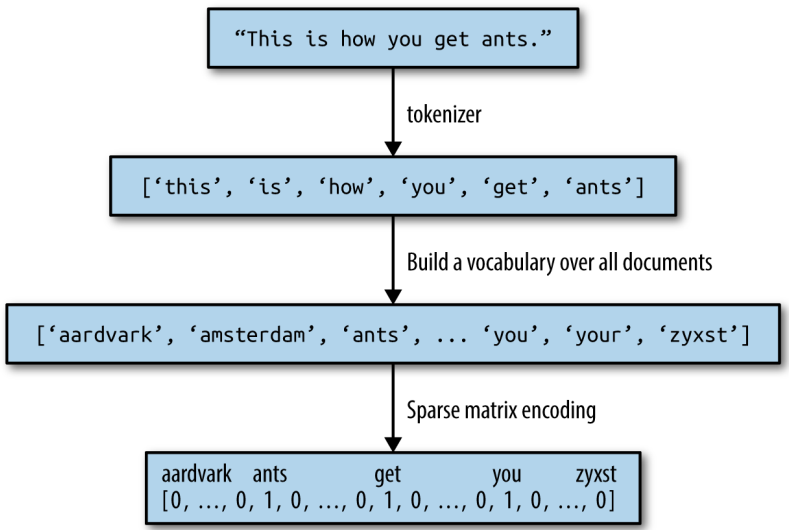
\includegraphics[scale=0.65]{Imagen_Machine/Texto2}
	\caption{Procesamiento de bolsa de palabras (bag-of-words)}
	\label{Texto2}
\end{figure}



\subsection{Aplicando Bag-of-Words en la dataset Toy}


La representación de la bolsa de palabras se implementa en {\ttfamily CountVectorizer}, que es un transformador. Para ver como  funciona lo aplicaremos sobre la  dataset Toy, que consta de dos muestras:

\begin{lstlisting}%[frame=single]

In[7]:
   
   bards_words =["The fool doth think he is wise,",
                 "but the wise man knows himself to be a fool"]
 
 \end{lstlisting}
 
 Importamos e instanciamos al {\ttfamily CountVectorizer} y ajustamos en la data Toy como sigue:
 
 \begin{lstlisting}%[frame=single]
 
  
In[8]:

   from sklearn.feature_extraction.text import CountVectorizer
   vect = CountVectorizer()
   vect.fit(bards_words)
   
    \end{lstlisting}
   
  El ajuste de {\ttfamily CountVectorizer} consiste en la tokenización de los datos de entrenamiento y la
  construcción del vocabulario, al que podemos acceder como el atributo {\ttfamily vocabulary\_}: 
   
   \begin{lstlisting}%[frame=single]
   
In[9]:

   print("Vocabulary size: {}".format(len(vect.vocabulary_)))
   print("Vocabulary content:\n {}".format(vect.vocabulary_))

Out[9]:

   Vocabulary size: 13
   Vocabulary content:
    {'the': 9, 'himself': 5, 'wise': 12, 'he': 4, 'doth': 2, 'to': 11, 
     'knows': 7,  'man': 8, 'fool': 3, 'is': 6, 'be': 0, 'think': 10,
     'but': 1}
   
    \end{lstlisting}
  
  El vocabulario consta de 13 palabras, desde "{}ser"{} ("{}be"{})  hasta "{}sabio"{} ("{}wise"{}). \\
  
  Para crear la representación de bolsa de palabras para los datos de entrenamiento, llamamos al método transformación   {\ttfamily transform:}  

 \begin{lstlisting}%[frame=single]

In[10]:

   bag_of_words = vect.transform(bards_words)
   print("bag_of_words: {}".format(repr(bag_of_words)))

Out[10]:

   bag_of_words: <2x13 sparse matrix of type '<class 'numpy.int64'>'
       with 16 stored elements in Compressed Sparse Row format>

\end{lstlisting}

La representación de la bolsa de palabrs (bag-of-words) se almacena en una matriz sparse de
SciPy que sólo almacena las entradas que no son cero (ver Capítulo \ref{Cap1} ). La matriz es de 
forma 2x13, con una fila para cada uno de los dos puntos de datos y una característica para
cada una de las palabras  del vocabulario.  
Se utiliza una matriz sparse (dispersa) ya que la  mayoría de los documentos sólo contienen un
 pequeño subconjunto de las palabras en el vocabulario, lo que significa que la mayoría de las  entradas en la matriz de características son 0.  Piense en cuántas palabras diferentes pueden aparecer en un comentario  de una película en comparación con todas las palabras en el idioma inglés (que es lo que modela el vocabulario).

Almacenar todos esos ceros sería improductivo, y un desperdicio de memoria. Para observar el
 contexto real de la matriz sparse, podemos convertirla en una matriz NumPy  "{}densa"{} 
(que también almacena todas las entradas 0) usando el método  {\ttfamily toarray}\footnote{Esto es posible porque estamos utilizando un data pequeña, Toy que contiene sólo 13 palabras. Para cualquier conjunto de datos real, esto daría lugar a un {\ttfamily MemoryError}.}:


\begin{lstlisting}%[frame=single]

In[11]:

   print("Dense representation of bag_of_words:\n{}".format(
          bag_of_words.toarray()))

Out[11]:

   Dense representation of bag_of_words:
   [[0 0 1 1 1 0 1 0 0 1 1 0 1]
    [1 1 0 1 0 1 0 1 1 1 0 1 1]]

\end{lstlisting}


Podemos ver que los recuentos de palabras para cada palabra son 0 o 1; ninguna de las dos cadenas en {\ttfamily bards\_words} contiene una palabra dos veces.

Echemos un vistazo a cómo leer estos vectores de características. La primera cadena ("{}El necio piensa que es sabio{}") ("{}The fool doth think he is wise"{})  se representa como la primera fila, y contiene la primera palabra en el vocabulario, "{}ser"{} ("{}be"{}), cero veces. También contiene la segunda palabra en el vocabulario, "{}pero"{} ("{}but"{}), cero veces. Contiene la tercera palabra, "{}doth"{}, una vez, y así sucesivamente. Observando ambas filas, podemos ver que la cuarta palabra, "{}tonto"{} ("{}fool"{}), la décima palabra, "{}el"{}  ("{}the"{}), y la decimotercera palabra, "{}sabio"{} ( "{}wise"{}), aparecen en ambas cadenas.

\subsubsection{Bolsa de palabras para las críticas de cine}

% Bag-of-Words for Movie Reviews

Ahora que hemos pasado por el proceso de la bolsa de palabras en detalle, vamos a aplicarlo 
a la tarea de análisis de sentimientos para las críticas de cine. Anteriormente, hemos
 cargado la data de entrenamiento y pruebas de las reseñas de IMDb en listas de cadenas 
 ({\ttfamily text\_train}  y  {\ttfamily  text\_test}), que ahora procesaremos:


\begin{lstlisting}%[frame=single]

In[12]:

   vect = CountVectorizer().fit(text_train)
   X_train = vect.transform(text_train)
   print("X_train:\n{}".format(repr(X_train)))

Out[12]:

   X_train:
   <25000x74849 sparse matrix of type '<class 'numpy.int64'>'
       with 3431196 stored elements in Compressed Sparse Row format>

\end{lstlisting}

La forma de {\ttfamily X\_train}, en la representación de la bolsa de palabras de los datos 
de entrenamiento, es de 25.000x74.849, lo que indica que el vocabulario contiene 74.849 
entradas. De nuevo, los datos se almacenan como una matriz sparse  SciPy. Echemos un 
vistazo al vocabulario con un poco más de detalle. Otra forma de acceder al vocabulario es 
utilizando el método {\ttfamily get\_feature\_name} del vectorizador, que devuelve una lista conveniente 
donde cada entrada corresponde a una característica: 


\begin{lstlisting}%[frame=single]

In[13]:

   feature_names = vect.get_feature_names()
   print("Number of features: {}".format(len(feature_names)))
   print("First 20 features:\n{}".format(feature_names[:20]))
   print("Features 20010 to 20030:\n{}".format(feature_names[20010:20030]))
   print("Every 2000th feature:\n{}".format(feature_names[::2000]))

Out[13]:

\end{lstlisting}

\vspace{-0.6cm}
\begin{figure}[h!]
%	\centering
	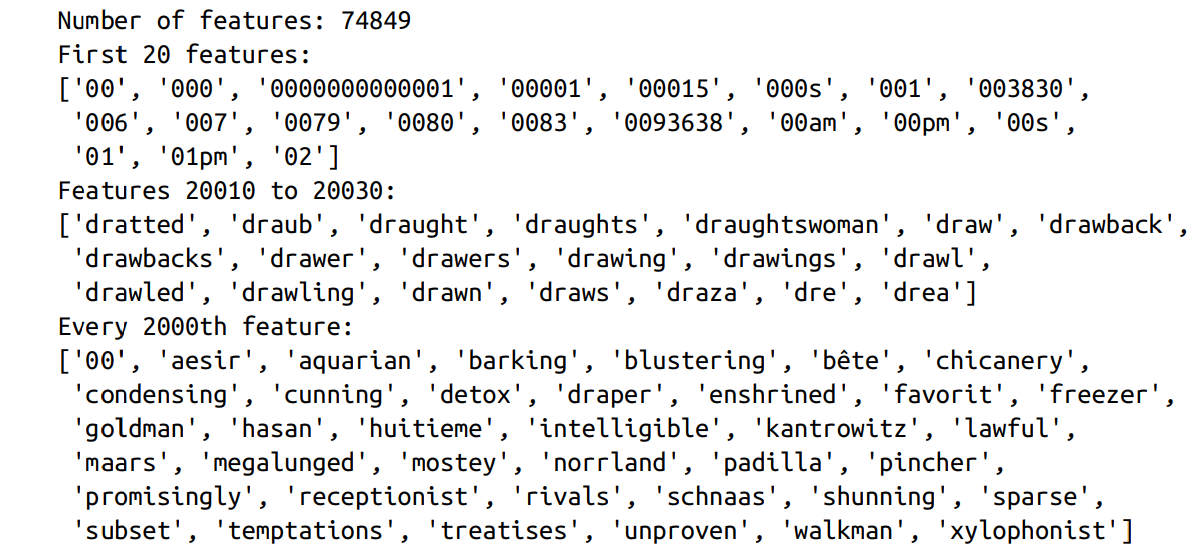
\includegraphics[scale=0.5]{Imagen_Machine/Out13}
%	\caption{Procesamiento de bolsa de palabras (bag-of-words)}
%	\label{Out13}
\end{figure}

Como puede ver, posiblemente un poco sorprendente, las primeras 10 entradas en el vocabulario son todas
números.   Todos estos números aparecen en algún lugar de las reseñas o comentarios,  y  por lo tanto, son
extraído como palabras. La mayoría de estos números no tienen ningún significado semántico inmediato: aparte de "007", que en el contexto particular de las películas es  probable que se refiera a  el personaje de James Bond\footnote{Un análisis rápido de los datos confirma que este es el caso. Intente confirmarlo usted.}. Eliminar lo significativo de las "{}palabras"{} no significativas es a veces difícil. Mirando más allá en el vocabulario,  encontramos una colección de palabras en inglés que comienzan con  con  "{}dra"{}. Puede notar que para  "{}draught, "{}drawback"{}, y  "{}drawer"  \: tanto la forma singular como la plural están contenidas en el  vocabulario como palabras distintas.  Estas palabras tienen significados semánticos estrechamente relacionados, y contarlos como diferentes palabras, correspondientes a diferentes características, podría no ser lo ideal.

%  "{}draught"{} ("{}borrador calado   redacto"{}),  "{}drawback"{} ("{}inconveniente"{}) y "{}drawback"{},  y "{}drawer"  ( "{}cajón"{} gaveta )
 

Antes de tratar de mejorar nuestra extracción de características, vamos a obtener una medida cuantitativa de rendimiento mediante la construcción de un clasificador. Tenemos las etiquetas de entrenamiento almacenadas en {\ttfamily y\_train}, y la representación de la bolsa de palabras de los datos de entrenamiento en {\ttfamily X\_train} para que podamos entrenar a un clasificador sobre estos datos. 
 Para datos de alta dimensión y sparse como este, los modelos lineales como {\ttfamily LogisticRegression} a menudo funcionan mejor.\\
 
Comencemos evaluando {\ttfamily LogisticRegresssion} usando validación cruzada\footnote{Usando la configuración predeterminada de {\ttfamily  CountVectorizer}, en realidad no recoge ninguna estadística, por lo que nuestros resultados son válidos. Usar Pipeline desde el principio sería una mejor opción para aplicaciones, pero lo diferimos para facilitar la exposición.}:


\begin{lstlisting}%[frame=single]

In[14]:

   from sklearn.model_selection import cross_val_score
   from sklearn.linear_model import LogisticRegression
   scores = cross_val_score(LogisticRegression(), X_train, y_train, cv=5)
   print("Mean cross-validation accuracy: {:.2f}".format(np.mean(scores)))

Out[14]:
    
    Mean cross-validation accuracy: 0.88
    
\end{lstlisting}

Obtenemos una puntuación media de validación cruzada del 88\%,  lo que indica un rendimiento 
razonable para una tarea de clasificación binaria balanceada. Sabemos que {\ttfamily LogisticRegression} 
tiene un parámetro de regularización C, que podemos ajustar mediante validación cruzada:

\begin{lstlisting}%[frame=single]

In[15]:

   from sklearn.model_selection import GridSearchCV
   param_grid = {'C': [0.001, 0.01, 0.1, 1, 10]}
   grid = GridSearchCV(LogisticRegression(), param_grid, cv=5)
   grid.fit(X_train, y_train)
   print("Best cross-validation score: {:.2f}".format(grid.best_score_))
   print("Best parameters: ", grid.best_params_)

Out[15]:
   
   Best cross-validation score: 0.89
   Best parameters: {'C': 0.1}

\end{lstlisting}

Obtenemos una puntuación de validación cruzada del 89\% utilizando $C = 0,1$. 
Ahora podemos evaluar la generalización del rendimiento de este ajuste de parámetro en el conjunto de prueba:


\begin{lstlisting}%[frame=single]

In[16]:

   X_test = vect.transform(text_test)
   print("{:.2f}".format(grid.score(X_test, y_test)))

Out[16]:

   0.88

\end{lstlisting}

Ahora, veamos si podemos mejorar la extracción de palabras.  Con la función  {\ttfamily CountVectorizer}
se extrae el tokens usando una expresión regular. Por defecto, la expresión regular que 
se usa es "{}$\setminus$b$\setminus$w$\setminus$w+$\setminus$b"{}.  
Si no está familiarizado con las expresiones regulares, esto significa que
busca todas las secuencias de caracteres que consisten  al menos dos letras o 
números ($\setminus$w) y que están separados por fonteras de palabras (word boundaries) ($\setminus$b). 
No encuentra palabras de una letra, y divide las contracciones como  “doesn’t{}”  o 
  “bit.ly{}”,  pero coincide  con "{}h8ter"{} como una sóla palabra,


 El {\ttfamily CountVectorizer} convierte todas las palabras en caracteres  minúscula, de modo que
“Soon”, “Soon” y “sOon” corresponden al mismo token (y, por lo tanto, la misma característica).
Este mecanismo simple funcionamuy bien en la práctica, pero como vimos anteriormente, obtenemos
muchas características no informativas (como los números). 

Una forma de reducir esto es  usar sólo tokens que aparezcan  al menos en dos documentos (o al menos en cinco documentos, y así sucesivamente). Un token que aparezca en un solo documento  es \emph{poco probable} que aparezca en el conjunto de pruebas y por lo tanto no es útil. Podemos configurar el número mínimo de documentos en un token debe aparecer con el parámetro {\ttfamily min\_df}:

\begin{lstlisting}%[frame=single]

In[17]:

   vect = CountVectorizer(min_df=5).fit(text_train)
   X_train = vect.transform(text_train)
   print("X_train with min_df:\n{}".format(repr(X_train)))

Out[17]:

   X_train with min_df:
    <25000x27271 sparse matrix of type '<class 'numpy.int64'>'
       with 3354014 stored elements in Compressed Sparse Row format>

\end{lstlisting}

Al requerir al menos cinco apariciones de cada token, podemos reducir el número de características a 27.271, como se ve en la salida anterior, sólo alrededor de un tercio de las características originales. Veamos algunas tokens de nuevo:

\begin{lstlisting}%[frame=single]

In[18]:

   feature_names = vect.get_feature_names()
   print("First 50 features:\n{}".format(feature_names[:50]))
   print("Features 20010 to 20030:\n{}".format(feature_names[20010:20030]))
   print("Every 700th feature:\n{}".format(feature_names[::700]))

Out[18]:
\end{lstlisting}

\vspace{-0.6cm}
\begin{figure}[h!]
	%\centering
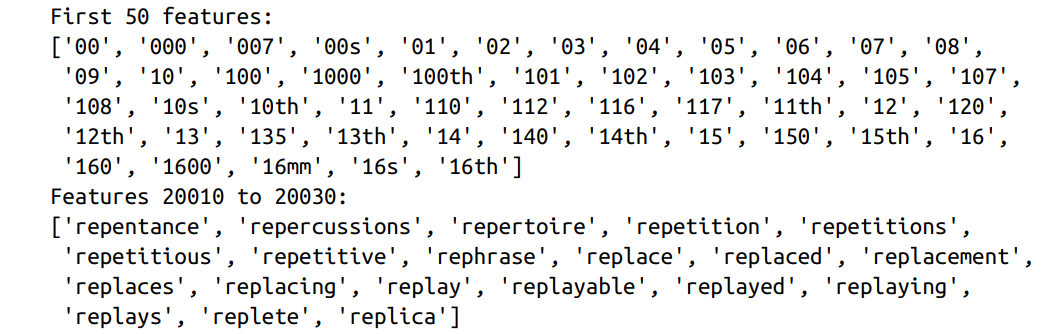
\includegraphics[scale=0.55]{Imagen_Machine/Out18a}
	%	\caption{Matriz de confusión para clasificación binaria}
	%	\label{Pipe3}
\end{figure}

\vspace{-0.9cm}
\begin{figure}[h!]
	%	\centering
	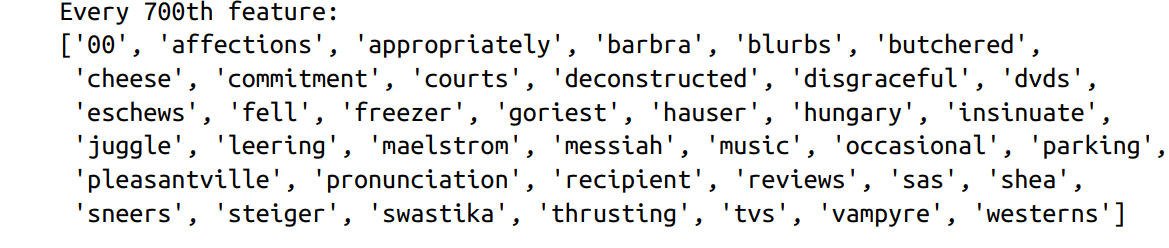
\includegraphics[scale=0.51]{Imagen_Machine/Out18b}
	%	\caption{Procesamiento de bolsa de palabras (bag-of-words)}
	%	\label{Out13}
\end{figure}

Claramente hay muchos menos números, y algunas de las palabras más oscuras o errores ortográficos
parecen haber desaparecido. Veamos qué tan bien funciona nuestro modelo repitiendo  una 
búsqueda por cuadrícula:


\begin{lstlisting}%[frame=single]

In[19]:

   grid = GridSearchCV(LogisticRegression(), param_grid, cv=5)
   grid.fit(X_train, y_train)
   print("Best cross-validation score: {:.2f}".format(grid.best_score_))

Out[19]:
   
   Best cross-validation score: 0.89

\end{lstlisting}

La mejor precisión de validación de la búsqueda en cuadrícula sigue siendo del 89\%, sin cambios desde antes. No mejoramos nuestro modelo, pero tener menos características para hacer frente a las velocidades de procesamiento y desechar características inútiles podría hacer el modelo más interpretable.\\

\begin{minipage}[t]{0.2\textwidth}
	\centering\raisebox{\dimexpr \topskip-\height}{%
		
\includegraphics[width=\textwidth]{Imagen_Machine/Pajaro}}
\end{minipage}%\hfill
\begin{minipage}[t]{0.75\textwidth} 
	{\scriptsize 		
		Si el método de transformación  {\ttfamily CountVectorizer} es llamado en un documento que 
		contiene palabras que no estaban contenidas en los datos de entrenamiento, esas palabras 
		serán ignoradas ya que no son parte del diccionario. Esto no es realmente un problema de clasificación, ya que no es posible aprender nada acerca de las palabras que no están en 
		los datos de entrenamiento. Para algunas aplicaciones, como la detección de spam, podría 
		ser útil añadir una característica que codifica cuántas palabras llamadas \:  "{}fuera de vocabulario"{} \: hay en un documento en particular. Para que esto funcione, es necesario establecer el mínimo con  {\ttfamily min\_df}; de lo contrario, esta característica nunca será activa durante el entrenamiento}
\end{minipage}\\


\subsection{Palabras vacías o Stopwords}

Otra forma para deshacernos de las palabras que no aportan información relevante
sobre el texto, conociadas como Stopwords\footnote{Las palabras que no aportan información relevante sobre el texto, se les conoce como Stopwords, o palabras vacías.}, consiste en desechar las palabras  que son demasiado frecuentes para ser informativas.  Hay dos enfoques principales: usar una lista específica de palabras clave, o descartar palabras que aparecen  con demasiada frecuencia.

 {\ttfamily scikit-learn} tiene una lista integrada de palabras  clave en inglés  en el módulo {\ttfamily feature\_extraction.text}:


\begin{lstlisting}%[frame=single]

In[20]:

   from sklearn.feature_extraction.text import ENGLISH_STOP_WORDS
   print("Number of stop words: {}".format(len(ENGLISH_STOP_WORDS)))
   print("Every 10th stopword:\n{}".format(list(ENGLISH_STOP_WORDS)[::10]))

Out[20]:

   Number of stop words: 318
   Every 10th stopword:
   ['above', 'elsewhere', 'into', 'well', 'rather', 'fifteen', 'had',
    'enough','herein', 'should', 'third', 'although', 'more', 'this',
    'none', 'seemed', 'nobody', 'seems', 'he', 'also', 'fill', 'anyone',
    'anything', 'me', 'the','yet', 'go', 'seeming', 'front','beforehand', 
    'forty', 'i']

\end{lstlisting}


Claramente, eliminando  las palabras  stopwords  en la lista sólo puede disminuir el número de 
características por la longitud de la lista 318, pero podría conducir a una 
mejora en el rendimiento. Veamos una  prueba:

\begin{lstlisting}

In[21]:

   # Specifying stop_words="english" uses the built-in list.
   # We could also augment it and pass our own.
   vect = CountVectorizer(min_df=5, stop_words="english").fit(text_train)
   X_train = vect.transform(text_train)
   print("X_train with stop words:\n{}".format(repr(X_train)))

Out[21]:

   X_train with stop words:
   <25000x26966 sparse matrix of type '<class 'numpy.int64'>'
       with 2149958 stored elements in Compressed Sparse Row format>

\end{lstlisting}

Ahora hay 305 (27.271-26.966) características menos en el conjunto de datos, lo que significa que la mayoría, pero no todas las palabras vacías (stopwords)  aparecieron. Vamos a ejecutar la búsqueda de cuadrícula 
(grid search)  nuevamente:  % appeared

\begin{lstlisting}%[frame=single]


In[22]:

   grid = GridSearchCV(LogisticRegression(), param_grid, cv=5)
   grid.fit(X_train, y_train)
   print("Best cross-validation score: {:.2f}".format(grid.best_score_))

Out[22]:

   Best cross-validation score: 0.88
\end{lstlisting}


El rendimiento de la búsqueda de cuadrícula disminuyó ligeramente usando  stopwords, no lo suficiente como para preocuparse, pero dado que excluir 305 características de más de 27.000 es poco probable que cambie mucho el rendimiento o la interpretabilidad, no parece que valga la pena usar esta lista. 

Las listas fijas son mayormente útiles para conjuntos de datos pequeños, que podrían no contener suficiente información para que el modelo determine qué palabras que son stopwords de los datos mismos. 
Como ejercicio, puede probar el otro enfoque, descartando palabras que aparecen con frecuencia, configurando la opción  {\ttfamily  max\_df}  de {\ttfamily CountVectorizer} y ver cómo influye en el número de características y el rendimiento.



\subsubsection{Re-escalando la data con {\ttfamily \bf{tf–idf}}}
%Rescaling the Data with tf–idf
% Reescalando los datos con tf – idf


En lugar de eliminar características que no se consideran importantes, otro enfoque es
reescalar las características según el nivel de información que esperamos que tengan.
Uno de los  formas más comunes de hacerlo es usado  el  método \emph{term frequency–inverse document frequency}  (tf-idf). 
La intuición de este método es dar mayor peso a cualquier término que aparezca
a menudo en un documento en particular, pero no en muchos documentos  del  corpus.
 Si una palabra aparece con frecuencia  en un documento en particular, pero no en muchos documentos, es probable que sea  muy descriptiva del contenido de ese documento. 
 {\ttfamily scikit-learn} implementa el método {\ttfamily tf–idf}  en dos clases:
  {\ttfamily TfidfTransformer}, que toma la matriz sparse de salida producida por 
   {\ttfamily CountVectorizer}  y los  transforma, y el {\ttfamily TfidfVectorizer}, 
 que toma la data  de texto y realiza tanto la extracción de características
 de bolsa de palabras como la   transformación {\ttfamily  tf–idf.}
  Hay algunas variantes  del esquema de reescalado  de  tf–df, sobre el cual  \href{https://en.wikipedia.org/wiki/Tf-idf}{\textcolor{vino}{puedes leer en Wikipedia} }.   

La puntuación  tf–idf   para la palabra \emph{w} en el documento  d
tal como se implementa en las clases {\ttfamily TfidfTransformer}  y  {\ttfamily TfidfVectorizer}   está dado por{\footnote{\scriptsize{Proporcionamos esta fórmula aquí principalmente para completar; pero no se necesita recordarla para usar la codificación tf-idf}}}:\\
 

 $ tfidf(w, d)  = tf \cdot log(\frac{N+1}{N_{w} + 1}) +1  $\\

\noindent donde N es el número de documentos en el conjunto de entrenamiento, $ N_{w} $ es el número de documentos en el conjunto de entrenamiento en el que aparece la palabra \emph{w}, y $tf$  el término frecuencia   es el cantidad de veces que la palabra \emph{w} aparece en el documento de consulta d (el documento que se quiere transformar o codificar).    
Ambas clases también aplican la normalización L2 después de calcular la representación  tf–idf; 
en otras palabras, reescalan la representación de cada documento para tener la norma 1 Euclidiana. 
Cambiar la escala de esta manera, significa que  la longitud de un documento{\footnote{\scriptsize{ La longitud de un documento es el número de palabras}}} no cambia la representación vectorizada.\\


Debido a que tf–idf en realidad hace uso de las propiedades estadísticas de los datos de entrenamiento,
utilizaremos  una  pipeline, como se describe en el Capítulo \ref{Cap6}, para garantizar que los resultados de la  búsqueda de cuadrícula sean  válidos. Esto lleva al siguiente código:

\begin{lstlisting}%[frame=single]

In[23]:

   from sklearn.feature_extraction.text import TfidfVectorizer
   from sklearn.pipeline import make_pipeline
   pipe = make_pipeline(TfidfVectorizer(min_df=5, norm=None),
                        LogisticRegression())                        
   param_grid = {'logisticregression__C': [0.001, 0.01, 0.1, 1, 10]}
   
   grid = GridSearchCV(pipe, param_grid, cv=5)
   grid.fit(text_train, y_train)
   print("Best cross-validation score: {:.2f}".format(grid.best_score_))

Out[23]:

   Best cross-validation score: 0.89

\end{lstlisting}


Como puedes ver, hay algunas mejoras al usar   \,tf-idf, \, en lugar de sólo contar palabras. 
También podemos inspeccionar qué palabras   encontró  tf-idf   más importantes. 
Tenga en cuenta que el escalado  \,tf-idf\, está destinado a encontrar palabras que distinguen los documentos, pero es una técnica puramente sin supervisión. 
Por lo tanto, lo "{}importante"{}  aquí no está necesariamente  relacionada con las etiquetas 
 "{}revisión positiva"{}  y  "{}revisión negativa"{}  que nos interesan. 
 En primer lugar, extraemos el {\ttfamily TfidfVectorizer} de la pipeline:

\begin{lstlisting}%[frame=single]

In[24]:

   vectorizer = grid.best_estimator_.named_steps["tfidfvectorizer"]
   # transform the training dataset
   X_train = vectorizer.transform(text_train)
   # find maximum value for each of the features over the dataset
   max_value = X_train.max(axis=0).toarray().ravel()
   sorted_by_tfidf = max_value.argsort()
   # get feature names
   feature_names = np.array(vectorizer.get_feature_names())
   
   print("Features with lowest tfidf:\n{}".format(
          feature_names[sorted_by_tfidf[:20]]))
   
   print("Features with highest tfidf: \n{}".format(
          feature_names[sorted_by_tfidf[-20:]]))

Out[24]:

   Features with lowest tfidf:
   ['poignant' 'disagree' 'instantly' 'importantly' 'lacked' 'occurred'
    'currently' 'altogether' 'nearby' 'undoubtedly' 'directs' 'fond' 'stinker'
    'avoided' 'emphasis' 'commented' 'disappoint' 'realizing' 'downhill'
    'inane']
   Features with highest tfidf:
   ['coop' 'homer' 'dillinger' 'hackenstein' 'gadget' 'taker' 'macarthur'
    'vargas' 'jesse' 'basket' 'dominick' 'the' 'victor' 'bridget' 'victoria'
    'khouri' 'zizek' 'rob' 'timon' 'titanic']
 
\end{lstlisting}


              % críticas   \, espacio pequeno ~ \: espacio mediano

Las características con bajo  \,tf-idf \,  son aquellas que se utilizan muy comúnmente en documentos
o sólo se utilizan con moderación, y sólo en documentos muy largos. Curiosamente, muchas de las características con un \, tf-idf  alto,  en realidad identificar ciertos espectáculos o películas.
Estos términos sólo aparecen en las reseñas de este espectáculo o franquicia en particular, 
pero tienden a aparecer muy a menudo en estas críticas particulares.  
Esto es muy claro, por ejemplo, para "{}pokemon"{}, "{}smallville"{} y "{}doodlebops"{}, pero "{}scanners"{}  aquí en realidad también se refiere a un título de película. 
Es poco probable que estas palabras nos ayuden en nuestra tarea de clasificación de sentimientos (a menos que tal vez algunas franquicias sean universalmente revisadas positiva o negativamente), pero ciertamente contienen mucha información específica sobre las reseñas, críticas o comentarios.\\


También podemos encontrar las palabras que tienen baja frecuencia inversa de documento, es decir, 
 aquellas que aparecen con frecuencia, y por lo tanto se consideran menos importantes. Los valores de frecuencia inversa de documento  encontrados en el conjunto de entrenamiento se almacenan en el atributo {\ttfamily idf\_}:


\begin{lstlisting}

In[25]:

   sorted_by_idf = np.argsort(vectorizer.idf_)
   print("Features with lowest idf:\n{}".format(
          feature_names[sorted_by_idf[:100]]))

Out[25]:

   Features with lowest idf:
   ['the' 'and' 'of' 'to' 'this' 'is' 'it' 'in' 'that' 'but' 'for' 'with'
    'was' 'as' 'on' 'movie' 'not' 'have' 'one' 'be' 'film' 'are' 'you' 'all'
    'at' 'an' 'by' 'so' 'from' 'like' 'who' 'they' 'there' 'if' 'his' 'out'
    'just' 'about' 'he' 'or' 'has' 'what' 'some' 'good' 'can' 'more' 'when'
    'time' 'up' 'very' 'even' 'only' 'no' 'would' 'my' 'see' 'really' 
    'story''which' 'well' 'had' 'me' 'than' 'much' 'their' 'get' 'were' 
    'other' 'been' 'do' 'most' 'don' 'her' 'also' 'into' 'first' 'made'
    'how' 'great' 'because' 'will' 'people' 'make' 'way' 'could' 'we' 'bad' 
    'after' 'any' 'too' 'then' 'them' 'she' 'watch' 'think' 'acting' 
    'movies' 'seen' 'its'  'him']

\end{lstlisting}

Como era de esperar, se trata en su mayoría de palabras clave en inglés como
 "{}the"{} y "{}no"{}. Pero algunos son claramente de dominio específico para las críticas de películas, 
 como "{}movie"{}, "{}film"{}, "{}time"{}, "{}story"{}, y así sucesivamente. 
 Curiosamente, las palabras "{}good"{}, "{}great"{}, y "{}bad"{}  también se encuentran entre las más frecuentes y    por lo tanto "{}menos relevantes"{} de acuerdo con la medida   tf-idf,   a pesar de que podríamos   esperar que estos sean muy importantes para nuestra tarea de análisis de sentimientos

\subsubsection{Análisis de los coeficientes modelo}

Finalmente, veamos un poco más en detalle lo que nuestro modelo de regresión logística
 realmente aprendió de los datos. Debido a que hay tantas características (27.271) después 
 de eliminar las infrecuentes,  claramente no puede ver todos los coeficientes al mismo tiempo. 
 Sin embargo, podemos ver  los coeficientes más grandes, y ver a qué palabras le corresponden estos. 
 Usaremos el último modelo que entrenamos, basado en las características de  tf-idf. 
El siguiente gráfico de barras (Figura \ref{Texto3}) muestra los 25 coeficientes más grandes y 25 más pequeños del modelo de regresión logística,  mostrando con las barras  el tamaño de cada coeficiente:


\begin{lstlisting}%[frame=single]

In[26]: 

   mglearn.tools.visualize_coefficients(
       grid.best_estimator_.named_steps["logisticregression"].coef_,
       feature_names, n_top_features=40)

\end{lstlisting}


\begin{figure}[h!]
	\centering
	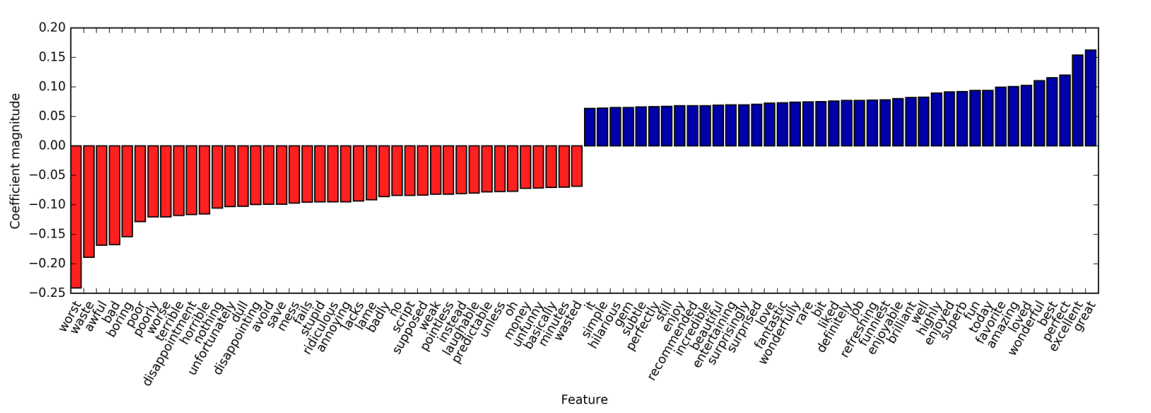
\includegraphics[scale=0.55]{Imagen_Machine/Texto3}
	\caption{Los coeficientes más grandes y más pequeños de las características de regresión logística
		 entrenados en tf-idf}
	\label{Texto3}
\end{figure}



Los coeficientes negativos a la izquierda pertenecen a palabras que según el modelo son indicativas de comentarios negativas, mientras que los coeficientes positivos a la derecha pertenecen a palabras que según el modelo indican comontarios positivos. La mayoría de los términos son bastante intuitivos, como "{}worst"{}, "{}waste"{}, "{}disappointment"{},  y  "{}laughable"{}  ("{}peor"{}, "{}desperdicio"{}, "{}decepción"{} y "{}ridículo"{})  que indica malas críticas de películas, mientras que "{}excellent"{}, "{}wonderful"{}, "{}enjoyable"{},  y 
"{}refreshing"{}  ("{}excelente"{}, "{}maravilloso"{}, "{}agradable"{} y "{}refrescante"{}) indican críticas positivas de películas.
 Algunas palabras son un poco menos claras, como "{}bit"{}, "{}job"{}, y "{}today"{}, pero estas podrían ser parte de frases como "{}good job"{} o "{}best today."{} 
 
\subsection{Bolsa de palabras con más de una palabra \\ (n-Grams)}


% Bag-of-Words with More Than One Word (n-Grams)

Una de las principales desventajas de usar una representación de bolsa de palabras es que el orden de las palabras se descarta por completo. Por lo tanto, las dos cadenas, "{}es malo, no es bueno en absoluto"{}  y  "{}es bueno, no es malo en absoluto"{}  \, tienen exactamente la misma representación, a pesar de que los significados están opuestos.
Poner "{}no"{}  delante de una palabra es sólo un ejemplo  de la  importancia del contexto. 
Afortunadamente, hay una manera de capturar el contexto cuando se utiliza una representación
de bolsa de palabras, no sólo considerando los recuentos de simples tokens, sino también
los recuentos de pares o triples de tokens que aparecen una al lado de la otra.

Los pares de tokens  se conocen como bigrams, los tripletas de tokens se conocen como trigramas, y más generalmente las secuencias de tokens se conocen como n-gramos.
Podemos cambiar el rango de tokens que son  considerados como características cambiando el parámetro {\ttfamily ngram\_range} \, de {\ttfamily CountVectorizer} o  {\ttfamily TfidfVectorizer}. 
El parámetro {\ttfamily  ngram\_range} es una tupla, que consistente en la longitud mínima y máxima de las secuencias de  tokens que son considerados. 

A continuación se expone  un ejemplo  sobre la data Toy  que utilizamos anteriormente:

\begin{lstlisting}%[frame=single]

In[27]:

   print("bards_words:\n{}".format(bards_words))

Out[27]:

   bards_words:
   ['The fool doth think he is wise,',
    'but the wise man knows himself to be a fool']
    
\end{lstlisting}

El valor por defecto  es crear una característica por secuencia de tokens que tenga al menos un token de  longitud  y a lo más un token de longitud, o en otras palabras, exactamente un token de logitud (los tokens individuales también se llaman unigramas):

\begin{lstlisting}%[frame=single]

In[28]:

   cv = CountVectorizer(ngram_range=(1, 1)).fit(bards_words)
   print("Vocabulary size: {}".format(len(cv.vocabulary_)))
   print("Vocabulary:\n{}".format(cv.get_feature_names()))

Out[28]:

   Vocabulary size: 13
   Vocabulary:
   ['be', 'but', 'doth', 'fool', 'he', 'himself', 'is', 'knows', 'man', 'the',
    'think', 'to', 'wise']

\end{lstlisting}

Para ver sólo a los bigrams; es decir, sólo a las secuencias de dos tokens que se suceden 
entre sí, podemos configurar un conjunto {\ttfamily ngram\_range} a (2, 2):

\begin{lstlisting}%[frame=single]

In[29]:

   cv = CountVectorizer(ngram_range=(2, 2)).fit(bards_words)
   print("Vocabulary size: {}".format(len(cv.vocabulary_)))
   print("Vocabulary:\n{}".format(cv.get_feature_names()))

Out[29]:
  
   Vocabulary size: 14
   Vocabulary:
   ['be fool', 'but the', 'doth think', 'fool doth', 'he is', 'himself to',
    'is wise', 'knows himself', 'man knows', 'the fool', 'the wise',
    'think he', 'to be', 'wise man']

\end{lstlisting}


El uso de secuencias más largas de tokens generalmente resulta en muchas más características,
y en características más específicas. No hay un bigram común entre las dos frases en
 {\ttfamily bard\_words}:


\begin{lstlisting}%[frame=single]

In[30]:

   print("Transformed data (dense):\n{}".format(
          cv.transform(bards_words).toarray()))

Out[30]:

   Transformed data (dense):
   [[0 0 1 1 1 0 1 0 0 1 0 1 0 0]
    [1 1 0 0 0 1 0 1 1 0 1 0 1 1]]

\end{lstlisting}

Para la mayoría de las aplicaciones, el número mínimo de tokens debe ser uno, 
como  palabras  únicas que con frecuencia capturan gran significado. Agregar un bigrams en 
la mayoría de los casos ayuda. 

Agregando secuencias más largas, hasta  5-grams, también pueden ayudar, pero esto conducirá 
a una explosión de la cantidad de características y podría conducir a un sobreajuste, 
ya que habrá muchas características específicas. 

En principio, el número de bigrams podría ser el número de unigrams al cuadrado y el número de trigrams podría ser el número de unigrams a la potencia de tres, lo que lleva a espacios de características muy grandes. En la práctica, el número alto de los n-grams  que realmente aparecen en los datos son mucho más pequeños, debido a la estructura  del idioma (inglés), aunque todavía es grande.

A continuación se muestra   como se ve el uso de unigrams, bigrams y trigrams sobre {\ttfamily bards\_words}:

\begin{lstlisting}%[frame=single]

In[31]:

   cv = CountVectorizer(ngram_range=(1, 3)).fit(bards_words)
   print("Vocabulary size: {}".format(len(cv.vocabulary_)))
   print("Vocabulary:\n{}".format(cv.get_feature_names()))

Out[31]:

   Vocabulary size: 39
   Vocabulary:
   ['be', 'be fool', 'but', 'but the', 'but the wise', 'doth', 'doth think',
    'doth think he', 'fool', 'fool doth', 'fool doth think', 'he', 'he is',
    'he is wise', 'himself', 'himself to', 'himself to be', 'is', 'is wise',
    'knows', 'knows himself', 'knows himself to', 'man', 'man knows',
    'man knows himself', 'the', 'the fool', 'the fool doth', 'the wise',
    'the wise man', 'think', 'think he', 'think he is', 'to', 'to be',
    'to be fool', 'wise', 'wise man', 'wise man knows']

\end{lstlisting}

Vamos a probar el {\ttfamily TfidfVectorizer} en los datos de comentarios de películas IMDb 
y encontrar la mejor configuración del rango  n-gram   utilizando una búsqueda de cuadrícula: 

\begin{lstlisting}%[frame=single]

In[32]:

   pipe = make_pipeline(TfidfVectorizer(min_df=5), LogisticRegression())
   # running the grid search takes a long time because of the
   # relatively large grid and the inclusion of trigrams
   param_grid = {"logisticregression__C": [0.001, 0.01, 0.1, 1, 10, 100],
                 "tfidfvectorizer__ngram_range": [(1, 1), (1, 2), (1, 3)]}
  
   grid = GridSearchCV(pipe, param_grid, cv=5)
   grid.fit(text_train, y_train)
   print("Best cross-validation score: {:.2f}".format(grid.best_score_))
   print("Best parameters:\n{}".format(grid.best_params_))

Out[32]:

   Best cross-validation score: 0.91
   Best parameters:
   {'tfidfvectorizer__ngram_range': (1, 3), 'logisticregression__C': 100}

\end{lstlisting}

Como se puede ver en los resultados, hemos mejorado el rendimiento un poco más que un 
por ciento mediante la adición características de  bigram  y  de trigrama. 
Podemos visualizar la exactitud (accuracy) de validación cruzada como una función 
del parámetro {\ttfamily ngram\_range} y C como un mapa caliente,   como se hizo en 
el capítulo \ref{Cap5} (ver Figura \ref{Texto4}):

\begin{lstlisting}%[frame=single]

In[33]:

   # extract scores from grid_search
   scores = grid.cv_results_['mean_test_score'].reshape(-1, 3).T
   # visualize heat map
   heatmap = mglearn.tools.heatmap(
       scores, xlabel="C", ylabel="ngram_range", cmap="viridis", fmt="%.3f",
       xticklabels=param_grid['logisticregression__C'],
       yticklabels=param_grid['tfidfvectorizer__ngram_range'])
   plt.colorbar(heatmap)

\end{lstlisting}

\begin{figure}[h!]
	\centering
	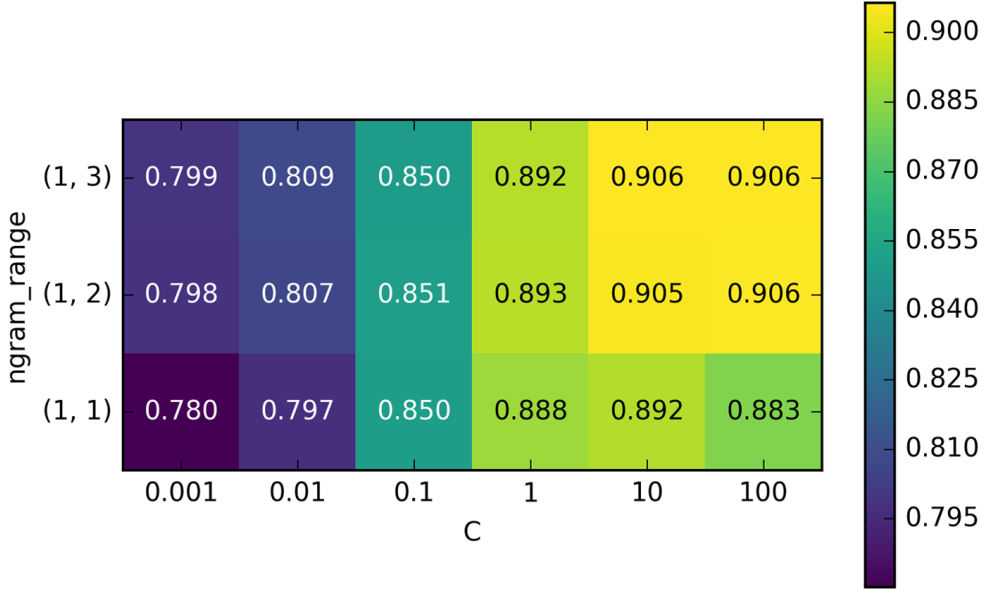
\includegraphics[scale=0.55]{Imagen_Machine/Texto4}
	\caption{Visualización del mapa caliente de la exactitud media de la validación cruzada como una función de los parámetros {\ttfamily ngram\_range} y C}
	\label{Texto4}
\end{figure}

En el  mapa caliente podemos ver que el uso de bigrams aumenta el rendimiento un poco, mientras que la adición de trigramas sólo proporciona un beneficio muy pequeño en términos de exactitud. Para entender mejor cómo mejoró el modelo, podemos visualizar la importancia de los coeficiente  para el mejor modelo, que incluye unigrams, bigrams y trigrams (ver Figura \ref{Texto5}):

\begin{lstlisting}%[frame=single]

In[34]:

   # extract feature names and coefficients
   vect = grid.best_estimator_.named_steps['tfidfvectorizer']
   feature_names = np.array(vect.get_feature_names())
   coef = grid.best_estimator_.named_steps['logisticregression'].coef_
   mglearn.tools.visualize_coefficients(coef, feature_names,
                                        n_top_features=40)

\end{lstlisting}

\begin{figure}[h!]
	\centering
	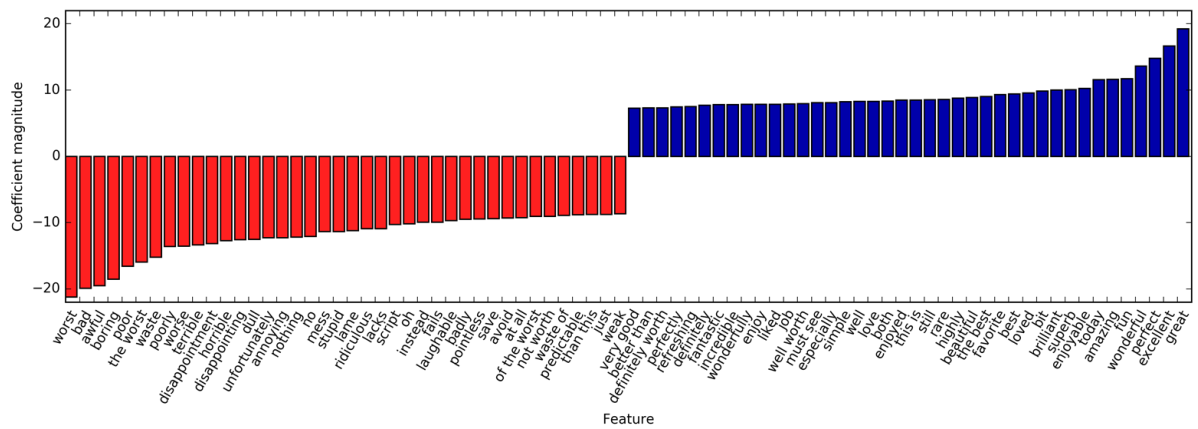
\includegraphics[scale=0.55]{Imagen_Machine/Texto5}
	\caption{Características más importantes al usar unigrams, bigrams y trigrams 
		con el reescalado  tf-idf}
	\label{Texto5}
\end{figure}

Hay características particularmente interesantes que contienen la palabra "{}worth"{} (valor)
que no estaban presentes en el modelo unigram: "{}not worth"{}  es indicativo de una comentario negativa, mientras que "{}definitely worth"{}  y "{}well worth"{}  son indicativos de una revisión positiva. 
Este es un primer ejemplo de contexto que influye en el significado de la palabra "{}worth"{}.


A continuación, visualizaremos sólo trigramas, para proporcionar una mayor comprensión de por qué estas características son útiles. Muchos de los bigrams y trigrams útiles consisten en palabras comunes que no serían informativos por sí solos, como en las frases "{}none of the"{},  "{}the only good"{}, "{}on and on"{}, "{}this is one"{}, "{}of the most"{} ("{}ninguno de los"{},  "{}el único bueno"{}, "{}incesantemente"{}, "{}esto es uno"{}, "{}de la mayoría"{}),  y así sucesivamente. 
Sin embargo, el impacto de estas características es bastante limitado en comparación con la importancia de las características de unigram, como se puede ver en la Figura \ref{Texto5}:

\begin{lstlisting}%[frame=single]

In[35]:

   # find 3-gram features
   mask = np.array(
           [len(feature.split(" "))  for feature in feature_names]) == 3
   # visualize only 3-gram features
   mglearn.tools.visualize_coefficients(
           coef.ravel()[mask],  feature_names[mask], n_top_features=40)

\end{lstlisting}

\begin{figure}[h!]
	\centering
	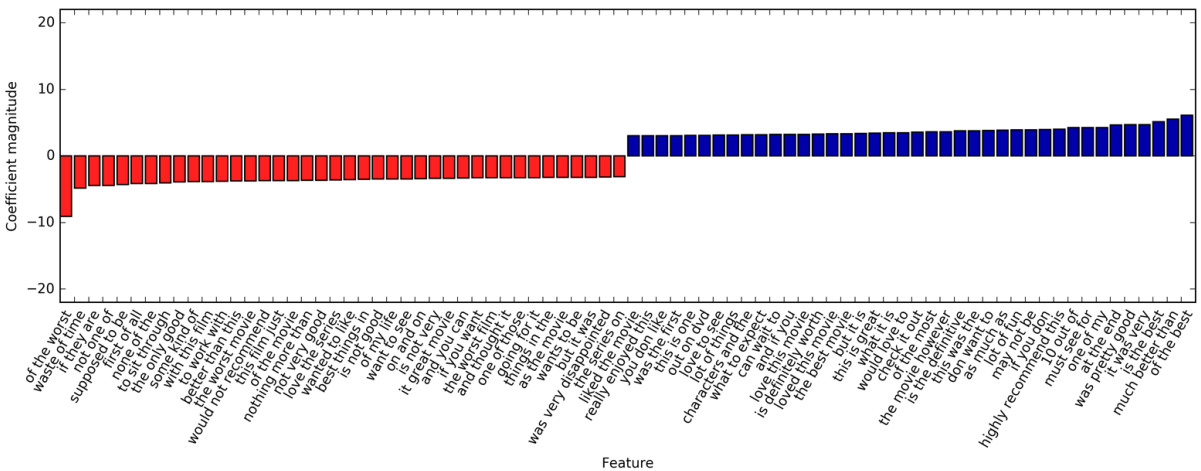
\includegraphics[scale=0.55]{Imagen_Machine/Texto7}
	\caption{Visualización  sólo de las características más importantes  del modelo trigram}
	\label{Texto7}
\end{figure}

\newpage
% siendo cada n-grama una secuencia de n palabras consecutivas
%  documentos del corpus (idf).
%  https://en.wikipedia.org/wiki/Lexical_analysis#Tokenization
%  https://towardsdatascience.com/why-you-should-avoid-removing-stopwords-aa7a353d2a52

\subsection{Tokenización avanzada,  Stemming y lematización}
%Como se mencionó anteriormente,

La extracción de características en {\ttfamily  CountVectorizer}  y  {\ttfamily TfidfVectorizer}  es relativamente simple, y   muchos métodos  más elaborados son posibles.
 Un paso particular que a menudo   mejora   las  aplicaciones de procesamiento de texto más sofisticadas,
es el primer paso en el modelo de bolsa de palabras: tokenización. Este paso define lo que
constituye una palabra para la extracción de características.\\


Vimos anteriormente que el vocabulario a menudo contiene versiones singulares y plurales de
algunas palabras, como en "{}inconveniente"{} y "{}inconvenientes"{}, "{}cajón"{} y "{}cajones"{}, y
"{}dibujo"{} y "{}dibujos"{}.   A los efectos de un modelo de bolsa de palabras, la semántica
de "{}inconveniente"{ }  y  "{}inconvenientes"{ } están tan cerca que distinguirlos sólo
aumentar el sobreajuste y no permiten que el modelo explote por completo 
los datos de entrenamiento.


Similarmente, encontramos que el vocabulario incluye palabras como "{}reemplazar"{},
 "{}reemplazado"{}, "{}reemplazadamente"{},  "{}reemplazos"{}  y  "{}reemplazando"{}, 
 que son formas verbales diferentes y un sustantivo relacionado con el verbo "{}reemplazar"{}.  
 De manera similar al tener formas singulares y plurales de un sustantivo, tratando  diferentes formas verbales y palabras relacionadas como símbolos distintos es desventajoso  para construir un modelo que generalice bien.\\

  
Este problema se puede superar representando cada palabra usando la raíz de la 
palabra\footnote{ \scriptsize{Raíz de una palabra: La parte común de las palabras se llama raíz, también 
	conocido como lexema. La raíz de una palabra es la parte de la palabra que no cambia. 
	A partir de una raíz podemos formar palabras que son relacionadas por su significado}} (word stem)
que involucra identificar (o combinar) todas las palabras que tienen la misma raíz.
 Si esto se realiza mediante el uso de una heurística basada en reglas, como descartar 
 sufijos comunes, generalmente es referido como stemming  (derivación).  Si, en cambio, se utiliza 
 un diccionario  de formas de palabras conocidas (un sistema explícito y verificado 
 por humanos), y  se toma  en cuenta el papel de la palabra en la oración, 
 el proceso se denomina lematización y la forma estandarizada de la palabra se 
 conoce como lema.  
Ambos métodos de procesamiento, lematización y stemming, son formas de normalización
  que intentan extraer alguna forma normal de una palabra.   Otro caso interesante de normalización es la corrección ortográfica, que puede ser
útil en la práctica pero está fuera del alcance de este libro.\\

Para obtener una mejor comprensión de la normalización, comparemos un método para stemming,
el método stemmer  Porter{\footnote{\scriptsize	{ algoritmo de Porter es un algoritmo que asegura que
 la forma de las palabras no penalice la frecuencia de éstas. Es decir, una palabra puede
  estar conjugada en cualquier género, número, persona, y solo se considerará como un solo término.}}}, 
una colección ampliamente utilizada de heurísticas (aquí importada del paquete {\ttfamily  nltk}) 
 para lemmatización como se implementa en el paquete {\ttfamily spacy}\footnote{ \scriptsize{ más detalles
 sobre la interfaz, consulte la documentación \href{http://www.nltk.org/}{\textcolor{vino}{\ttfamily nltk} }} y \href{https://spacy.io/}{\textcolor{vino}{\ttfamily spacy} }. Aquí sólo nos interesamos en los principios generales.}:


\begin{lstlisting}%[frame=single]

In[36]:

   import spacy
   import nltk
   
   # load spacy's English-language models
   en_nlp = spacy.load('en')
   # instantiate nltk's Porter stemmer
   stemmer = nltk.stem.PorterStemmer()
   
   # define function to compare lemmatization in spacy with stemming in nltk
   def compare_normalization(doc):
       # tokenize document in spacy
       doc_spacy = en_nlp(doc)
       # print lemmas found by spacy
       print("Lemmatization:")
       print([token.lemma_ for token in doc_spacy])
       # print tokens found by Porter stemmer
       print("Stemming:")
       print([stemmer.stem(token.norm_.lower()) for token in doc_spacy])

\end{lstlisting}

Vamos a comparar lemmatización y el stemmer Porter en una frase diseñada para mostrar algunas de las diferencias:

\begin{lstlisting}%[frame=single]

In[37]:

   compare_normalization(u"Our meeting today was worse than yesterday, "
   "I'm scared of meeting the clients tomorrow.")

Out[37]:

   Lemmatization:
   ['our', 'meeting', 'today', 'be', 'bad', 'than', 'yesterday', ',', 'i',
    'be', 'scared', 'of', 'meet', 'the', 'client', 'tomorrow', '.']
   Stemming:
   ['our', 'meet', 'today', 'wa', 'wors', 'than', 'yesterday', ',', 'i', 
    'm', 'scare', 'of', 'meet', 'the', 'client', 'tomorrow', '.']

\end{lstlisting}

Stemming está siempre  restringido  a recortar la palabra a una stem (raíz), así que "{}was"{} 
se convierte en "{}wa"{}, mientras que la lemmatización puede recuperar la forma de
 base del verbo  correcta, "{}be"{}. De manera similar, la lemmatización puede normalizar  
 "{}worse"{}  a "{}bad"{}  ( "{}peor"{} a "{}malo"{}), mientras que stemming 
  produce  "{}wors"{}. 
Otra diferencia importante es que stemming  reduce ambos casos  "{}meeting"{ } a
"{}meet"{ }   ("{}reunión"{}  a "{}reunirse"{}).
 Usando lematización, la primera ocurrencia  de  "{}meeting"{}   ("{}reunión"{})  se reconoce
  como un sustantivo y se deja como está, mientras que la segunda ocurrencia se reconoce como un 
 verbo y se reduce a  "{}meet"{} ("{}reunión"{}).  \\


En general, la lemmatización es un proceso mucho más complicado que el stemming, 
pero generalmente produce mejores resultados  que el stemming cuando se utiliza 
para  normalización  los tokens de aprendizaje automático.\\


Mientras que {\ttfamily scikit-learn} no implementa ninguna forma de normalización, {\ttfamily CountVectorizer} permite especificar su propio tokenizador  para convertir cada documento 
en una lista de tokens usando el parámetro {\ttfamily tokenizer}. 
Podemos usar la lematización de {\ttfamily spacy} para crear un invocable que tomará una 
cadena y producirá una lista de lemas:




\begin{lstlisting}%[frame=single]

In[38]:

   # Technicality: we want to use the regexp-based tokenizer
   # that is used by CountVectorizer and only use the lemmatization
   # from spacy. To this end, we replace en_nlp.tokenizer 
   # (the spacy tokenizer) with the regexp-based tokenization.
   import re
   # regexp used in CountVectorizer
   regexp = re.compile('(?u)\\b\\w\\w+\\b')
   
   # load spacy language model and save old tokenizer
   en_nlp = spacy.load('en')
   old_tokenizer = en_nlp.tokenizer
   # replace the tokenizer with the preceding regexp
   en_nlp.tokenizer = lambda string: old_tokenizer.tokens_from_list(
       regexp.findall(string))
   
   # create a custom tokenizer using the spacy document processing
   #  pipeline
   # (now using our own tokenizer)
   def custom_tokenizer(document):
       doc_spacy = en_nlp(document, entity=False, parse=False)
       return [token.lemma_ for token in doc_spacy]
       
   # define a count vectorizer with the custom tokenizer
   lemma_vect = CountVectorizer(tokenizer=custom_tokenizer, min_df=5)

\end{lstlisting}

Transformemos los datos e inspeccionemos el tamaño del vocabulario:

\begin{lstlisting}%[frame=single]

In[39]:

   # transform text_train using CountVectorizer with lemmatization
   X_train_lemma = lemma_vect.fit_transform(text_train)
   print("X_train_lemma.shape: {}".format(X_train_lemma.shape))
   
   # standard CountVectorizer for reference
   vect = CountVectorizer(min_df=5).fit(text_train)
   X_train = vect.transform(text_train)
   print("X_train.shape: {}".format(X_train.shape))

Out[39]:

   X_train_lemma.shape: (25000, 21596)
   X_train.shape: (25000, 27271)

\end{lstlisting}

\noindent Como se puede ver en la salida, el método lemmatización redujo el número de 
características de 27.271 (con el procesamiento {\ttfamily CountVectorizer estándar}) 
a 21.596. La lemmatización puede ser vista como una tipo de regularización, ya que combina
 ciertas características.
 Por lo tanto, esperamos que la lemmatización mejore el rendimiento más cuando la data es pequeña.
 Para ilustrar cómo la lemmatización puede ayudar, usaremos {\ttfamily StratifiedShuffleSplit} para la validación cruzada, usando solo el 1\% de los datos para conjunto de entrenamiento y el resto como datos de prueba:

\begin{lstlisting}%[frame=single]

In[40]:

   # build a grid search using only 1% of the data as the training set
   from sklearn.model_selection import StratifiedShuffleSplit
   
   param_grid = {'C': [0.001, 0.01, 0.1, 1, 10]}
   cv = StratifiedShuffleSplit(n_iter=5, test_size=0.99,
                               train_size=0.01, random_state=0)
   grid = GridSearchCV(LogisticRegression(), param_grid, cv=cv)
   # perform grid search with standard CountVectorizer
   grid.fit(X_train, y_train)
   print("Best cross-validation score "
         "(standard CountVectorizer): {:.3f}".format(grid.best_score_))
   # perform grid search with lemmatization
   grid.fit(X_train_lemma, y_train)
   print("Best cross-validation score "
         "(lemmatization): {:.3f}".format(grid.best_score_))

Out[40]:

   Best cross-validation score (standard CountVectorizer): 0.721
   Best cross-validation score (lemmatization): 0.731

\end{lstlisting}

En este caso, la lemmatización proporcionó una modesta mejora en el desempeño.
 Al igual que con muchas de las diferentes técnicas de extracción de características,
 el resultado varía dependiendo de la dataset. 
 
 La lemmatización y el stemming a veces  pueden ayudar a construir modelos mejores (o al menos más compactos), por lo que le   sugerimos que pruebe estas técnicas  tratando de exprimir la última gota 
  de rendimiento en una tarea en particular.

\subsection{Modelado de temas y Clúster de documentos}

Una técnica particular que a menudo se aplica a los datos de texto es el
 modelado de temas o tópicos, que es un término general  que describe la tarea de 
 asignar cada documento a uno o varios temas, por lo general sin supervisión. 
 Un buen ejemplo de este caso  son los datos noticiosos, que podrían clasificarse en
 temas como "política", "deportes", "finanzas", etc. Si a cada documento se le 
 asigna un sólo tema, esta es la tarea de agrupar los documentos, como se discute
 en el Capítulo \ref{Cap3}. 
Si cada documento puede tener más de un tema,  
la tarea se relaciona con los métodos de descomposición del Capítulo \ref{Cap3}.  Cada uno de los componentes  aprendidos  corresponde a un tema, y los coeficientes de los componentes en la representación de un documento nos dicen lo fuerte que es  la  relación del documento con un tema en particular. A menudo, cuando la gente habla de modelado de temas, se refieren a un método de descomposición parcial llamado \emph{Asignación de Dirichlet latente} (Latent Dirichlet Allocation, LDA)\footnote{Hay otro modelo de aprendizaje automático que también se abrevia a como LDA: Linear Discriminant Analysis, un modelo de clasificación lineal. Esto lleva a bastante confusión. En este libro, LDA se refiere a la Asignación Dirichlet Latente.}.


\subsection{Asignación de Latente  Dirichlet  LDA} 
%Latent Dirichlet Allocation

Intuitivamente, el modelo LDA intenta encontrar grupos de palabras (los temas) que aparecen frecuentemente juntos. LDA también requiere que cada documento pueda ser entendido como una "{}mezcla"{}  de un subconjunto de los temas. Es importante entender que para el modelo de aprendizaje automático un "{}tema"{} podría no ser lo que normalmente llamaríamos un tema en el discurso diario, pero que se asemeja más a los componentes extraídos por  PCA  o  NMF (que discutimos en el capítulo \ref{Cap3}), que puede o no tener un significado semántico.

Incluso si hay un significado semántico para un "{}tema"{ }  de  LDA, puede que no sea algo que normalmente llamamos un tema.   Volviendo al ejemplo de los artículos de noticias, podríamos
tener  una colección de artículos sobre deportes, política y finanzas, escritos por dos
autores. En un artículo sobre política, podríamos esperar ver palabras como "{}gobernador"{}, "{}votar"{}
"{}Fiesta"{}, etc., mientras que en otro artículo de deportes podemos esperar palabras como "{}equipo"{}, "{}puntuación"{}  y  "{}temporada."{} 
Sin embargo, estos no son los únicos grupos de palabras que podríamos esperar que aparezcan juntas.
Los dos reporteros podría preferir diferentes frases o diferentes opciones de palabras. 
 Quizás a uno de ellos le guste utilizar la palabra "{}demarcar"{} y a el otro le gusta la palabra "{}polarizar"{}.  Otros "{}temas"{} serían "{}palabras de uso frecuente por el reportero A"{}  y  "{}palabras de uso frecuente por el reportero B"{},  aunque estos no son temas en el sentido habitual de la palabra. \\


Vamos a aplicar LDA a la data reseñas de peliculas (review  movie) para ver cómo 
funciona en la práctica. Para los modelos de documentos de texto sin supervisión, a menudo es bueno eliminar palabras muy comunes, ya que de lo contrario podrían dominar el análisis. Eliminaremos las palabras que aparecen  al menos en un 15 por ciento de los documentos, y limitaremos el modelo de bolsa de palabras (bag-of-words) a las 10.000 palabras que son más comunes después de eliminar un  máximo de  15 por ciento: 

\begin{lstlisting}%[frame=single]

In[41]:

   vect = CountVectorizer(max_features=10000, max_df=.15)
   X = vect.fit_transform(text_train)
   
\end{lstlisting}

Vamos a entrenar el aprendizaje  de  un modelo  con 10 tópicos (temas), que son pocos y suficiente
 como para que podamos verlos  a todos. De manera similar a los componentes en  NMF, 
los temas no tienen un orden inherente, y cambiar el número de temas cambiará todos los temas\footnote{De hecho, NMF y LDA resuelven problemas muy relacionados, y también podríamos utilizar NMF para extraer temas}.  Usaremos el método de aprendizaje "{}por lotes"{} ("{}batch"{}),  que es algo más lento 
que el predeterminado  ("{}online"{}),  pero por lo general proporciona mejores resultados, y aumentar  el \:  "{}{\ttfamily max\_iter}"{}    también puede conducir a mejores modelos:

\begin{lstlisting}%[frame=single]

In[42]:

   from sklearn.decomposition import LatentDirichletAllocation
   lda = LatentDirichletAllocation(n_topics=10, learning_method="batch",
                                   max_iter=25, random_state=0)
   # We build the model and transform the data in one step
   # Computing transform takes some time,
   # and we can save time by doing both at once
   document_topics = lda.fit_transform(X)
   
\end{lstlisting}

Al igual que los métodos de descomposición que vimos en el capítulo \ref{Cap3}, {\ttfamily LatentDirichletAllocation}  tiene un atributo {\ttfamily components\_} que almacena la
 importancia de cada palabra para cada tema. El tamaño de  {\ttfamily components\_} \: es  
 {\ttfamily (n\_topics, n\_words)}:

\begin{lstlisting}%[frame=single]

In[43]:
   
   lda.components_.shape

Out[43]:
   
   (10, 10000)

\end{lstlisting}

Para entender mejor lo que significan los diferentes temas, veremos las palabras más 
importantes para cada uno de los temas. La función {\ttfamily print\_topics}  proporciona un 
formato agradable para estas características:


%%%%%%%%%%%%%%%%%%%%%%%%%%%%%%%%%%%%%%%%%%%%%%%%%%%%%%%%%%%%%%%
%%  Aqui va In[44]
%%%%%%%%%%%%%%%%%%%%%%%%%%%%%%%%%%%%%%%%%%%%%%%%%%%%%%%%%%%%%%%


\begin{lstlisting}%[frame=single]

In[44]:

   # For each topic (a row in the components_), sort the features (ascending)
   # Invert rows with [:, ::-1] to make sorting descending
   sorting = np.argsort(lda.components_, axis=1)[:, ::-1]
   # Get the feature names from the vectorizer
   feature_names = np.array(vect.get_feature_names())

In[45]:

   # Print out the 10 topics:
   mglearn.tools.print_topics(topics=range(10), feature_names=feature_names,
                              sorting=sorting, topics_per_chunk=5, n_words=10)

Out[45]
\end{lstlisting}
\vspace{-0.45cm}
\begin{figure}[h!]
	%	\centering
	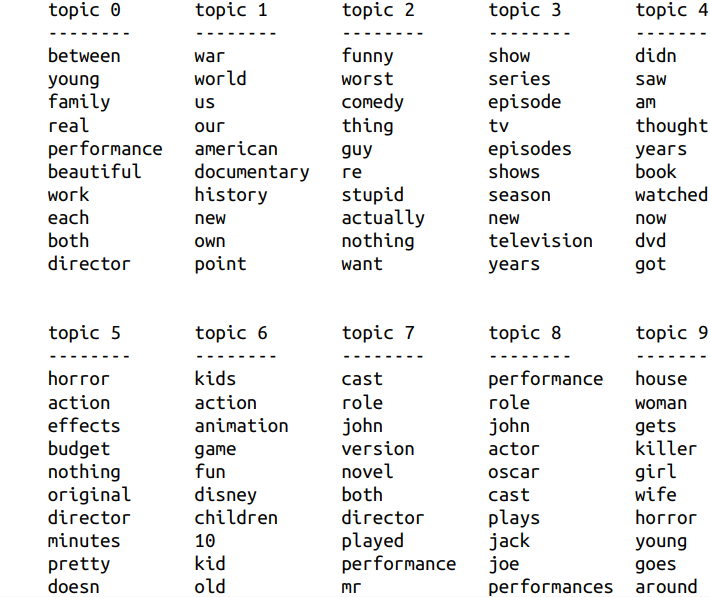
\includegraphics[scale=0.65]{Imagen_Machine/Out44}
	%\caption{Matriz de confusión para clasificación binaria}
	%	\label{Out44}
\end{figure}

\newpage 
Juzgando por las palabras importantes, el tema 1 parece ser sobre películas históricas y de guerra (bélicos), el tema 2 podría ser sobre malas comedias, el tema 3 podría ser sobre series de televisión. El tema 4 parece capturar algunas palabras muy comunes, mientras que el tema 6 parece ser sobre sobre películas infantiles  y el tema 8 parece capturar críticas relacionadas con premios. Utilizando sólo 10 temas, cada uno de los temas tiene que ser muy amplio, para que juntos puedan cubrir todos los diferentes tipos de comentarios  en la dataset.\\


A continuación, se entrena otro modelo de aprendizaje, esta vez con 100 temas. El uso de más temas hace el análisis mucho más difícil, pero hace más probable que los temas puedan   especializarse en subconjuntos interesantes de la data:

%%%%%%%%%%%%%%%%%%%%%%%%%%%%%%%%%%%%%%%%%%%%%%%%%%%%%%%%%%%%%%%
%%  Aqui no  va In[44]
%%%%%%%%%%%%%%%%%%%%%%%%%%%%%%%%%%%%%%%%%%%%%%%%%%%%%%%%%%%%%%%

\begin{lstlisting}%[frame=single]


In[46]:

   lda100 = LatentDirichletAllocation(n_topics=100, learning_method="batch",
                                      max_iter=25, random_state=0)
   document_topics100 = lda100.fit_transform(X)


\end{lstlisting}

\noindent   Observando todos los 100 temas sería un poco abrumador, así que seleccionamos algunos temas de interés y representativos:

\begin{lstlisting}%[frame=single]


In[47]:

   topics = np.array([7, 16, 24, 25, 28, 36, 37, 45, 51, 53, 54, 63, 89, 97])
   
   sorting = np.argsort(lda100.components_, axis=1)[:, ::-1]
   feature_names = np.array(vect.get_feature_names())
   mglearn.tools.print_topics(topics=topics, feature_names=feature_names,
                              sorting=sorting, topics_per_chunk=7, n_words=20)

Out[47]:

\end{lstlisting}    %   error Out[48]
\vspace{-0.65cm}
\begin{figure}[h!]
	%	\centering
	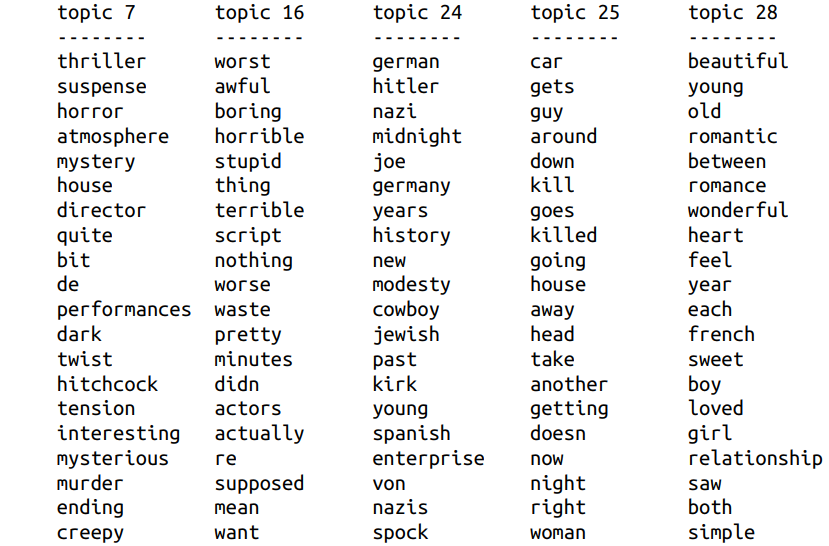
\includegraphics[scale=0.55]{Imagen_Machine/Out48}
	%\caption{Matriz de confusión para clasificación binaria}
	%	\label{Out48}
\end{figure}

\vspace{-3.5cm}
\begin{figure}[h!]
	%	\centering
	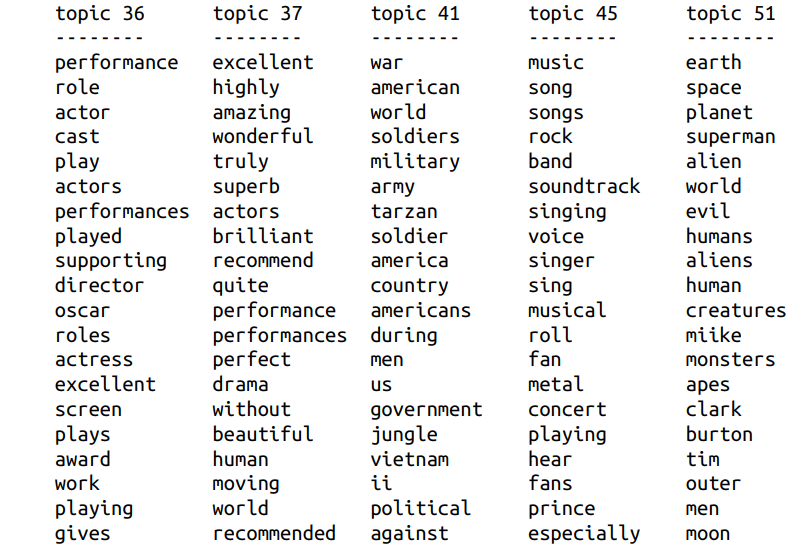
\includegraphics[scale=0.55]{Imagen_Machine/Out48a}
	%\caption{Matriz de confusión para clasificación binaria}
	%	\label{Out48b}
\end{figure}
\vspace{-0.5cm}\hspace{-0.9cm}
\begin{minipage}[t]{1\textwidth}
	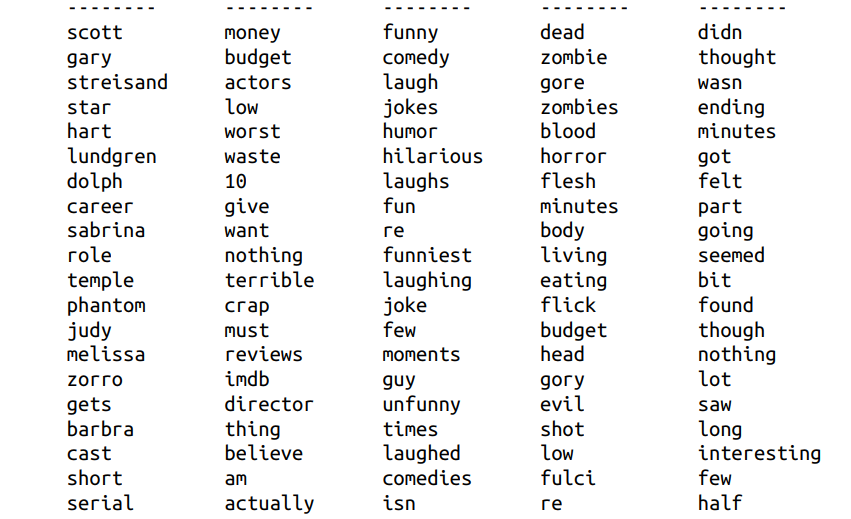
\includegraphics[scale=0.55]{Imagen_Machine/Out48b}
\end{minipage}


Los temas que hemos extraído esta vez parecen ser más específicos, aunque muchos son difíciles de interpretar. El tema 7 parece versar sobre películas de terror y suspenso (thrillers); los temas 16 y 54 parecen captar malas críticas, mientras que el tema 63 en su mayoría parece captar críticas positivas de comedias. Si queremos hacer más inferencias usando los temas que fueron descubiertos, debemos confirmar la intuición que ganamos al ver las palabras de mayor rango  para cada tema observando los documentos que se asignan a estos temas. Por ejemplo, al tema 45 parece versar sobre la música. Vamos a comprobar qué tipos de reseñas se asignan a este tema:


\begin{lstlisting}

In[49]:
   
   # sort by weight of "music" topic 45
   music = np.argsort(document_topics100[:, 45])[::-1]
   # print the five documents where the topic is most important
   for i in music[:10]:
   # pshow first two sentences
   print(b".".join(text_train[i].split(b".")[:2]) + b".\n")

Out[49]:

   b'I love this movie and never get tired of watching. The music in it is 
     great.\n'
   b"I enjoyed Still Crazy more than any film I have seen in years. A 
     successful band from the 70's decide to give it another try.\n"
   b'Hollywood Hotel was the last movie musical that Busby Berkeley 
     directed  for Warner Bros. His directing style had changed or
     evolved to the point that this film does not contain his 
     signature overhead shots or huge production numbers with thousands 
     of extras.\n'
   b"What happens to washed up rock-n-roll stars in the late 1990's?
     They launch a comeback / reunion tour. At least, that's what the
     members of Strange Fruit, a (fictional) 70's stadium rock group do.\n"
   b'As a big-time Prince fan of the last three to four years, I really 
     can\'t believe I\'ve only just got round to watching "Purple Rain". 
     The brand  new  2-disc anniversary Special Edition led me to buy it.\n'
   b"This film is worth seeing alone for Jared Harris' outstanding portrayal
     of John Lennon. It doesn't matter that Harris doesn't exactly resemble
     Lennon; his mannerisms, expressions, posture, accent and attitude are
     pure Lennon.\n"
   b"The funky, yet strictly second-tier British glam-rock band Strange 
     Fruit breaks up at the end of the wild'n'wacky excess-ridden 70's. The 
     individual band members go their separate ways and uncomfortably settle
     into lackluster middle age in the dull and uneventful 90's: morose 
     keyboardist Stephen Rea winds up penniless and down on his luck, vain, 
     neurotic, pretentious lead singer Bill Nighy tries (and fails) to
     pursue a floundering solo career, paranoid drummer Timothy Spall 
     resides in obscurity on a remote farm so he can avoid paying a hefty 
     back taxes debt, and surly bass player Jimmy Nail installs roofs for 
     a living.\n"
   b"I just finished reading a book on Anita Loos' work and the photo in TCM
     Magazine of MacDonald in her angel costume looked great 
     (impressive wings), so I thought I'd watch this movie. I'd never heard 
     of the film before, so I had no preconceived notions about it 
     whatsoever.\n"
   b'I love this movie!!! Purple Rain came out the year I was born and it
     has had my heart since I can remember. Prince is so tight in this 
     movie.\n'
   b"This movie is sort of a Carrie meets Heavy Metal. It's about a 
     highschool guy who gets picked on alot and he totally gets revenge with
     the help of a Heavy Metal ghost.\n"

\end{lstlisting}


Como podemos ver, este tema cubre una amplia variedad  de comentarios centrados en música, desde comedias musicales, a películas biográficas, para  algún  género difícil de especificar   en el último comentario.   Otra forma interesante para inspeccionar los tópicos,   es ver cuánto peso se le da a cada tema,   sumando  todos tópicos  {\ttfamily  document\_topics}  de todas las  reseñas.  Nombramos cada tema por las dos palabras más comunes. En la  figura \ref{LDA8} se muestran las ponderaciones tópicos  aprendidos:


\begin{lstlisting}%[frame=single]

In[50]:

   fig, ax = plt.subplots(1, 2, figsize=(10, 10))
   topic_names = ["{:>2} ".format(i) + " ".join(words)
                 for i, words in enumerate(feature_names[sorting[:, :2]])]
   # two column bar chart:
   for col in [0, 1]:
       start = col * 50
       end = (col + 1) * 50
       ax[col].barh(np.arange(50), 
                    np.sum(document_topics100, axis=0)[start:end])
       ax[col].set_yticks(np.arange(50))
       ax[col].set_yticklabels(topic_names[start:end], ha="left", va="top")
       ax[col].invert_yaxis()
       ax[col].set_xlim(0, 2000)
       yax = ax[col].get_yaxis()
       yax.set_tick_params(pad=130)
   plt.tight_layout()

\end{lstlisting}

\begin{figure}[h!]
	\centering
	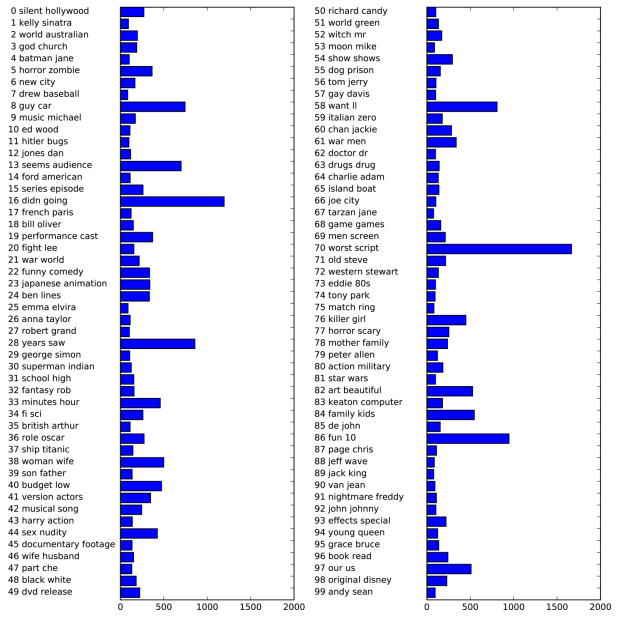
\includegraphics[width=1.03\textwidth]{Imagen_Machine/Texto8}
	\caption{Pesos temáticos aprendidos por LDA}
\label{LDA8}
\end{figure}


De acuerdo con el gráfico de la figura \ref{LDA8}, los temas más importantes son 97, que parece consistir principalmente en stopwords (palabras vacías), posiblemente  con una ligera dirección negativa; el tema 16,  claramente trata sobre malas críticas;
seguido de algunos temas específicos de género, el  36 y 37, ambos parecen contener palabras elogiosas.\\

Parece que LDA descubrió principalmente dos tipos de temas,  género específico y específica valoración
 (genre-specific y ratingspecific), además de varios temas   poco  específicos.   Este es un descubrimiento interesante, ya que la mayoría de las reseñas están hechas  por algunos comentarios específicos de películas y algunos  que justifican o enfatizan la valoración (rating).
   
Los modelos de temas como LDA son métodos interesantes para comprender grandes corpus de texto en
la ausencia de etiquetas,  o  como aquí, incluso si hay etiquetas disponibles. 
El algoritmo LDA es aleatorizado, sin embargo,  cambiar el parámetro 
 {\ttfamily random\_state} puede conducir resultados muy diferentes.


 Si bien identificar temas puede ser útil, cualquier conclusión que saques de un modelo no supervisado debe tomarse con un grano de sal, y recomendamos verificar tu intuición observando los documentos en un tema específico. 
 Los temas producidos por el método {\ttfamily LDA.transform}  también pueden utilizarse a veces como una representación conjunta para el aprendizaje supervisado. Esto es particularmente útil cuando se dispone de pocos ejemplos para entrenar.



\section{Resumen y perspectivas}


En este capítulo hemos introducido algunos   conceptos básicos del procesamiento de texto, también conocido como  procesamiento natural  del lenguaje (PNL), con  ejemplo de   aplicación   que clasifica críticas de películas. 
Las herramientas discutidas aquí deberían servir como un excelente punto de partida
 al tratar de procesar datos de texto. En particular para tareas de clasificación de texto, como detección de spam y fraude o análisis de sentimientos, las representaciones en bolsa de palabras proporcionan una forma simple y poderosa solución.    Como suele ser el caso en el aprendizaje automático, la representación de los datos es clave
en aplicaciones de PNL, e inspeccionando los tokens y n-grams   que  se  extraen y pueden
brindar información valiosa sobre el proceso de modelado.  En aplicaciones de procesamiento de texto, con frecuencia es posible introspectar   (inspección interna)  modelos de manera significativa, como vimos en este capítulo, para tareas supervisadas y no supervisadas.  Deberías aprovechar al máximo esta habilidad cuando se utilizan métodos basados PNL en la práctica.\\


El lenguaje natural y el procesamiento de textos es un gran campo de investigación; sin embargo, 
discutir los detalles de los métodos avanzados está mucho más allá del alcance de este libro.
Si quieres aprender más, recomendamos el libro  O’Reilly  \href{https://www.oreilly.com/library/view/natural-language-processing/9780596803346/}{\textcolor{vino}{ Natural Language Processing} }  con Python por Steven Bird, Ewan Klein y Edward Loper, que proporciona una visión general del  PNL junto con una introducción al paquete {\ttfamily nltk}  de Python para PNL. 
Otro buen libro más conceptual es la referencia estándar \href{https://nlp.stanford.edu/IR-book/}{\textcolor{vino}{Introduction to Information Retrieval} }
por Christopher Manning, Prabhakar Raghavan e Hinrich Schütze, que describe
algoritmos fundamentales en recuperación de información, PNL y aprendizaje automático. Ambos
los libros tienen versiones en línea a las que se puede acceder de forma gratuita.

Las clases {\ttfamily CountVectorizer}  y  {\ttfamily fidfVectorizer} sólo se implementan relativamente a métodos simples   de procesamiento de texto. Para métodos de procesamiento de texto más avanzados,  
se recomienda  los paquetes de Python {\ttfamily spacy} (un paquete relativamente nuevo pero muy  
eficiente y bien diseñado), {\ttfamily nltk} (una biblioteca muy bien establecida y completa pero algo antigua), y {\ttfamily gensim} (un paquete de PNL con énfasis en el modelado de temas). 
 {\ttfamily spacy}   y {\ttfamily gensim,}  Ambos    proporcionan funcionalidad para las técnicas 
discutidas  en  este  documento. \\

En los últimos años se han producido varias novedades muy interesantes en el procesamiento de textos,
que están fuera del alcance de este libro y se relacionan con las redes neuronales.
Uno  es el uso de representaciones vectoriales continuas, también conocidas como vectores
 de palabras o representaciones de palabras distribuidas, como se implementa en la libreria {\ttfamily word2vec}.    El documento original  \href{http://papers.nips.cc/paper/5021-di}{\textcolor{vino}{"{}Distributed Representations of Words and Phrases and  Their Compositionality"{ }} } por Thomas Mikolov et al. Es una gran introducción  al tema. 
   \\

 
 Otra dirección en el PNL que ha cobrado impulso en los últimos años
es el uso de redes neuronales recurrentes (RRNs) para el procesamiento de textos.
Las RRNs son un tipo particularmente potente de red neuronal que puede producir 
{\bf una salida que es de nuevo texto}, en contraste con los modelos de clasificación que sólo pueden asignar
etiquetas de clase. 

La capacidad de producir texto como salida hace que  RNNs sea muy adecuado para 
la traducción automática y resumen.  Una introducción al tema se puede encontrar en el artículo relativamente técnico \href{http://papers.nips.cc/paper/5346-sequence-to-sequence-learning-with-neural-networks.pdf}{\textcolor{vino}{"{}Sequence to 	Sequence Learning with Neural Networks"{}} } de Ilya Suskever,
Oriol Vinyals y Quoc Le.
 Un tutorial más práctico usando el marco {\ttfamily tensorflow}  se puede 
encontrar en el 
\href{https://www.tensorflow.org}{\textcolor{vino}{"{}sitio web de tensorflow"{}} }.








%%%%%%%%%%%%%%%%%%%%%%%%%%%%%%





   
   


















\chapter{Consejos y conclusiones}


Ahora sabes cómo aplicar los algoritmos de aprendizaje automático importantes para el 
aprendizaje supervisado y no supervisado,  que le permiten resolver una amplia variedad 
de problemas de aprendizaje automático. Antes de dejarte para explore  todas las posibilidades 
que ofrece el aprendizaje automático, queremos darte unas últimas palabras de consejo, 
apuntarte hacia algunos recursos adicionales y darte sugerencias sobre cómo puedes
mejorar aún más tus habilidades de aprendizaje automático y ciencia de datos.\\



\section{Abordando un problema de aprendizaje automático}
	

Con todos los  métodos que introducimos  en este libro y que ahora tiene al alcance de su mano,
 puede ser tentador saltar y comenzar a resolver  problemas relacionados con los datos 
simplemente ejecutando configurando su algoritmo favorito. Sin embargo, esta no suele ser una buena forma de comenzar su análisis. El algoritmo de aprendizaje automático suele ser sólo una pequeña parte de 
 una larga lista de etapas del proceso de análisis de datos y toma de decisiones.
  Para hacer un uso efectivo del aprendizaje automático, necesitamos  dar un paso atrás y considerar el problema en general. Primero, debes  pensar sobre el tipo de pregunta que desea responder. 

¿Quiere hacer un análisis exploratorio y ver si encuentra algo interesante en los datos?
¿O ya tienes un objetivo en particular en mente?  
En general,   se comienza  con un objetivo claro, como detectar transacciones fraudulentos
 de usuarios, recomendaciones de películas o búsqueda de planetas desconocidos. 
 Si tiene tal objetivo, antes de construir un sistema para lograrlo, primero debe pensar
sobre cómo definir y medir el éxito, y cuál es el impacto de una solución exitosa
de su objetivo general de investigación o negocio.

  Supongamos  que su objetivo es detectar fraudes, entonces surgen las siguientes preguntas:

\begin{list}{$\bullet$}{}  
	
	\item  ¿Cómo medir si la predicción de fraude realmente está funcionando?
	
	\item ¿Tengo la data correcta para evaluar con un algoritmo?
	
	\item  Si tengo éxito, ¿cuál será el impacto comercial de mi solución?
	
\end{list}

Como se discutió  en el Capítulo \ref{Cap5}, es mejor si puede medir el desempeño del
algoritmo utilizando directamente una métrica empresarial, como aumento de ganancias o disminución de pérdidas. Sin embargo, esto no es tan sencillo de hacer. 

Una pregunta que puede ser más fácil de responder es  "{}¿Qué pasa si construyó el modelo perfecto? "{} 
Si detectar perfectamente cualquier fraude le ahorrará a la empresa \$ 100 al mes, estos posibles ahorros probablemente no serán suficientes para garantizar el esfuerzo de empezar a desarrollar un algoritmo.  Por otro lado, si el modelo pudiera ahorrarle a su empresa decenas de miles de dólares cada mes, el problema podría ser vale la pena explorar.\\
	

Supongamos que se ha definido el problema a resolver, conocemos una solución  que 
puede tener un  impacto  significado   para el  proyecto, y se ha asegurado de tener
la información correcta para evaluar el éxito. Los siguientes pasos generalmente son 
adquirir los datos y crear un prototipo.\\
 
En este libro hemos tratado  muchos modelos que se pueden emplear,  cómo para evaluar y ajustar correctamente estos modelos.   Sin embargo, mientras se prueban los modelos, se debe tener muy presente  que esto es sólo una pequeña parte de un gran flujo de trabajo de ciencia de datos, y la construcción de los  modelos a menudo es parte de un círculo de retroalimentación de {\emph{ recolección  de nuevos datos, limpieza de datos, construcción modelos y análisis de  modelos.}}   
Analizar los errores que comete un modelo con frecuencia puede ser informativo sobre lo que 
falta en los datos, qué datos adicionales podrían ser seleccionado, 
o cómo se podría reformular la tarea para hacer que el aprendizaje automático sea más efectivo.
Recopilar más o diferentes datos o cambiar ligeramente la formulación de la tarea podría
proporcionan una recompensa   mayor  que realizar búsquedas interminables en la red para ajustar los parámetros.	

\subsection{Los seres humanos en el bucle}

También debe considerar si debe tener humanos en el circuito y cómo.   Algunos procesos (como la detección de peatones en un coche auto-conducido) necesitan tomar decisiones inmediatas.
Otros podrían no necesitar respuestas inmediatas, por lo que puede ser posible que los seres humanos confirmen decisiones inciertas.  Las aplicaciones médicas, por ejemplo, pueden necesitar niveles muy altos de precisión  que posiblemente no se puedan lograr con solo un algoritmo de aprendizaje automático. 

Pero si un algoritmo puede generar 90 por ciento, 50 por ciento o tal vez incluso
sólo el 10 por ciento de las decisiones de forma automática, eso ya podría aumentar el tiempo de respuesta
o reducir el costo.  Muchas aplicaciones están dominadas por "{}casos simples"{}, para los cuales un algoritmo puede tomar una decisión, con relativamente pocos "{}casos complicados"{}, que pueden ser
redirigido a un humano.
	
\subsection{Del prototipo a la producción}

Las herramientas que analizamos en este libro son excelentes para muchas aplicaciones de aprendizaje automático,  permiten análisis y creación de prototipos muy rápidos.
Python y {\ttfamily scikit-learn} se utiliza también   en sistemas de producción en muchas organizaciones, incluso en grandes organizaciones como  bancos internacionales y empresas globales de redes sociales. Sin embargo, muchas empresas tienen una infraestructura compleja, y no siempre es fácil incluir Python en estos sistemas.  
Esto no es necesariamente un problema. En muchas empresas, los equipos de análisis de datos
trabajar con lenguajes como Python y R que permiten la prueba rápida de ideas, mientras
los equipos de producción trabajan con lenguajes como Go, Scala, C\!{\scriptsize ++}  y Java para crear
sistemas robustos y  escalables.  El análisis de datos tiene  diferentes requisitos  en la creación de servicios en vivo,
por lo que tiene sentido usar diferentes lenguajes para estas tareas. Una solucón 
relativamente común  es volver a implementar la solución que encontró el equipo 
de análisis interno al marco más grande, utilizando un lenguaje de alto rendimiento. 
Esto puede ser más fácil que incrustar una librería  completa o lenguaje de programación
 y convertir desde y hacia los diferentes formatos de datos.\\



Independientemente de si puede usar {\ttfamily scikit-learn}  en un sistema de producción o no, es importante tener en cuenta que los sistemas de producción tienen requisitos diferentes de los scripts de análisis únicos.

Si un algoritmo se implementa en un sistema más grande, los aspectos de ingeniería de software como confiabilidad,  predictibilidad, tiempo de ejecución y requisitos de memoria ganan relevancia.

La simplicidad es clave para proporcionar sistemas de aprendizaje automático que funcionan bien en estas áreas. Inspeccione críticamente cada parte del proceso de datos y la  predicción de  pipeline y pregúntese cuánta complejidad crea cada paso, qué tan robusta es cada componente a los cambios en los datos o la infraestructura de cómputo, y si el beneficio de cada componente justifica la complejidad.



Si  está involucrando sistemas de   aprendizaje automático, recomendamos encarecidamente leer el artículo \href{https://research.google/pubs/pub43146/}{\textcolor{vino}{"{}Machine Learning: The High Interest Credit Card of Technical Debt"{}}}, publicado por el equipo de investigadores en Google de aprendizaje automático. 
El documento destaca la compensación en la creación y el mantenimiento de software de aprendizaje automático en producción a gran escala. Si bien el tema de la deuda técnica es particularmente apremiante en proyectos a gran escala y a largo plazo, las lecciones aprendidas pueden ayudarnos a crear un mejor software incluso para sistemas más pequeños y de corta duración.\\

\subsection{Probando sistemas de producción}




 En este libro, cubrimos cómo evaluar predicciones algorítmicas basadas en un conjunto de pruebas que recopilamos de antemano. Esto se conoce como  \emph{evaluación fuera de línea}. Si su sistema de aprendizaje automático es orientado al usuario, este es sólo el primer paso en la evaluación de un algoritmo, sin embargo; el siguiente paso es generalmente pruebas en línea o pruebas en vivo, donde se evalúan las consecuencias de emplear el algoritmo en el sistema en general. 
Cambiar las recomendaciones o resultados de búsqueda de los usuarios que se muestran por un sitio web puede cambiar drásticamente su comportamiento y conducir a consecuencias inesperadas.  Para protegerse  contra estas sorpresas, la mayoría de los servicios orientados al usuario emplean pruebas A/B, una forma de estudio de usuarios ciegos.


En las pruebas A/B, sin su conocimiento, una parte seleccionada de los usuarios recibirá
un sitio web o servicio que utiliza el algoritmo A, mientras que al resto de usuarios se les proporcionará
con el algoritmo B. Para ambos grupos, las métricas de éxito relevantes se registrarán en un conjunto de 
período de tiempo. Luego, se compararán las métricas del algoritmo A y el algoritmo B,
y se realizará una selección entre los dos enfoques de acuerdo con estas métricas.

El uso de pruebas A/B nos permite evaluar los algoritmos "{}en estado salvaje"{}, lo que podría ayudarnos a descubrir consecuencias inesperadas cuando los usuarios interactúan con nuestro modelo.
Con frecuencia, el modelo nuevo es A, mientras que B es el sistema establecido.  Hay mecanismos más elaborados para las pruebas en línea que van más allá de las pruebas A/B, como los algoritmos de bandidos. Una gran introducción a este tema se puede encontrar en el libro  \href{http://shop.oreilly.com/product/0636920027393.do}{\textcolor{vino}{ Bandit Algorithms for Website Optimization}} de John Myles White (O'Reilly).



\subsection{Construyendo su propio estimador} 

Este libro ha cubierto una variedad de herramientas y algoritmos implementados en {\ttfamily scikit-learn} que ser usado en una amplia gama de tareas. Sin embargo, con gran frecuencia siempre  habrá algún procesamiento particular que necesiten  sus datos y que no está implementado en{\ttfamily scikit-learn}. 
Puede ser suficiente para preprocesar sus datos antes de pasarlos a su modelo {\ttfamily scikit-learn} o pipeline. Sin embargo, si su preprocesamiento depende de los datos, y desea aplicar una búsqueda de cuadrícula o validación cruzada, las cosas se vuelven más complicadas.\\

En el  Capítulo \ref{Cap6}  discutimos la importancia de poner todo el procesamiento dependiente de datos
dentro del ciclo de validación cruzada. Entonces, ¿cómo puede usar su propio procesamiento junto con las herramientas de {\ttfamily scikit-learn}?     Implementar un estimador que sea compatible con la interfaz de {\ttfamily scikit learn}, para que pueda usarse con  {\ttfamily Pipeline, GridSearchCV}  y {\ttfamily cross\_val\_score}, es muy fácil. 
Puede encontrar instrucciones detalladas en la \href{https://scikit-learn.org/stable/developers/contributing.html#rolling-your-own-estimator}{\textcolor{vino}{documentación de  {\ttfamily scikit-learn}}}, pero aquí está la esencia.
La forma más sencilla de implementar una clase transformer   es heredando de {\ttfamily BaseEstimator} y {\ttfamily TransformerMixin}, y luego implementando las funciones {\ttfamily \_\_init\_\_, fit y predict} como la siguiente:





\begin{lstlisting}%[frame=single]

In[1]:

   from sklearn.base import BaseEstimator, TransformerMixin
   
   class MyTransformer(BaseEstimator, TransformerMixin):
       def __init__(self, first_parameter=1, second_parameter=2):
           # All parameters must be specified in the __init__ function
           self.first_parameter = 1
           self.second_parameter = 2
         
       def fit(self, X, y=None):
           # fit should only take X and y as parameters
           # Even if your model is unsupervised, you need to accept a y argument!
          
           # Model fitting code goes here
           print("fitting the model right here")
           # fit returns self
           return self
          
      def transform(self, X):
          # transform takes as parameter only X
          # Apply some transformation to X
          X_transformed = X + 1
          return X_transformed
         
\end{lstlisting}


Implementar un clasificador o regresor funciona de manera similar, solo que en lugar de 
{\ttfamily TransformerMixin} necesitas heredar de {\ttfamily ClassifierMixin}  o {\ttfamily  RegressorMixin}. Además, en lugar de implementar {\ttfamily transform} , se implementaría { \ttfamily predict}.

 Como se puede ver en el ejemplo dado aquí, la implementación de su propio estimador requiere muy poco código, y la mayoría de los usuarios de  {\ttfamily scikit-learn}  crean una colección de modelos personalizados a lo largo del tiempo.
 
 
 
\subsection{Dónde ir desde aquí}
%   Where to Go from Here
 
 Este libro proporciona una introducción al aprendizaje automático y le hará un profesional eficiente.
  Sin embargo, si desea mejorar sus habilidades de aprendizaje automático, aquí hay  sugerimos algunos  libros y recursos más especializados para investigar más a fondo


\subsection{Teoría} 

En este libro, tratamos de proporcionar una intuición de cómo funcionan los algoritmos de aprendizaje automático más comunes, sin requerir una base sólida en matemáticas o ciencias de la computación. Sin embargo, muchos de los modelos que discutimos utilizan principios de la teoría de probabilidad, álgebra lineal y optimización. Si bien no es necesario entender todos los detalles de cómo se implementan estos algoritmos, creemos que conocer algo de la teoría detrás de los algoritmos te hará un mejor científico de datos.


Se han escrito muchos libros buenos sobre la teoría del aprendizaje automático,
y si pudiéramos entusiasmarlo con las posibilidades que abre el aprendizaje automático,
 le sugerimos que elija al menos uno de ellos y profundice. 
 Ya  hemos mencionado el libro de Hastie, Tibshirani y Friedman The Elements of Statistical Learning el el 
prefacio, pero vale la pena repetir aquí esta recomendación. 
Otro libro muy  accesible, con el código de Python que lo acompaña, es Machine Learning: An Algorithmic Perspective de Stephen Marsland (Chapman y Hall{\scriptsize/}CRC). 
Otros dos clásicos muy recomendados son Pattern Recognition y Machine Learning de Christopher Bishop (Springer), un libro que hace hincapié en un marco probabilístico, y Machine Learning; y el libro de   A Probabilistic Perspective de Kevin Murphy (MIT Press), una completa  disertación (leer:1,000{\scriptsize+} páginas) sobre métodos de aprendizaje automático con debates en profundidad sobre los enfoques más avanzados, mucho más allá de lo que podríamos cubrir en este libro.


\subsection{Otros marcos y paquetes de aprendizaje automático}


Si bien   {\ttfamily scikit-learn}  es nuestro paquete favorito para el aprendizaje automático{\footnote{Andreas podría no ser totalmente objetivo en este asunto.}} y Python es nuestro
lenguaje favorito para el aprendizaje automático, existen muchas otras opciones.
Dependiendo de sus necesidades, Python y {\ttfamily scikit-learn}  pueden no ser la mejor opción para
tu situación particular. 
Generalmente, usar Python es ideal para probar y evaluar modelos, pero los servicios web y aplicaciones más grandes se escriben  comúnmente en Java  o  C{\scriptsize++}, y  la integración en estos sistemas puede ser necesaria para que su modelo sea desplegado.
Otra razón por la que puede querer ir más allá de {\ttfamily scikit-learn},   es si  su interés es el modelado estadístico y la inferencia,  más  que en la predicción. 
En este caso, debería considerar el paquete {\ttfamily statsmodel } de Python, que implementa varios modelos lineales con una interfaz pensada con  más enfasiss en estadística.  
Si no esta casado con Python, también puede considerar el uso de R, otra lengua franca de los científicos de datos. R es un lenguaje diseñado específicamente para el análisis estadístico y es famoso por sus excelentes capacidades de visualización y la disponibilidad de un gran número  de paquetes para modelado estadístico (generalmente altamente especializados).\\


Otro paquete de aprendizaje automático muy popular es {\ttfamily vowpal wabbit} 
(llamado  {\ttfamily vw } para evitar la posible distorsión de la lengua), un paquete
de aprendizaje automático altamente optimizado escrito en  C{\scriptsize++}   con una interfaz de 
línea de comandos.   {\ttfamily vw} es particularmente útil para grandes conjuntos de datos y
para la transmisión de datos. Para ejecutar algoritmos de aprendizaje automático distribuidos sobre un clúster, una de las soluciones más populares en el momento de escribir este artículo es {\ttfamily mllib}, una librería Scala construida sobre el entorno de computación distribuida de Spark.



\subsection{Ranking, sistemas de recomendación y otros tipos de aprendizaje}
 

Debido a que este es un libro introductorio, nos hemos centramos en las tareas más comunes de aprendizaje automático: clasificación y regresión en el aprendizaje supervisado,  clúster y
descomposición de señales en el aprendizaje no supervisado. Hay muchos más tipos de aprendizaje automático, con muchas aplicaciones importantes.  Dos tópicos  particularmente importantes que no cubrimos en este libro; son  el Ranking  y los sistemas de recomendación. El ranking  en que queremos recuperar las respuestas de una  consulta en particular, ordenadas por su relevancia.  probablemente ya haya utilizado un sistema  ranking hoy; así es como  operan los motores de búsqueda. Ingresa una consulta de búsqueda y obtiene una lista ordenada de respuestas, clasificadas por su relevancia (ranked).   Una  introducción a la   clasificación ranking se encuentra en el   libro de Schütze {\ttfamily{Introduction to Information Retrieval}} por   Manning, Raghavan, y  Schütze’s.     El segundo tópico son los sistemas de recomendación, que brindan sugerencias a los  usuarios en función de sus preferencias. Probablemente haya encontrado sistemas de recomendación bajo títulos como "{}Personas que puede conocer"{},  "{}Los clientes que compraron este artículo también compraron"{}  o  "{}Mejores selecciones para Usted."{} 
Hay un montón de literatura sobre el tema, y si tiene interés, puede visitar la web de  
\href{http://www.netflixprize.com/}{\textcolor{vino}{ "{}Netflix prize challeng"{} } }
  ("{}Desafío de premios de Netflix"{}),  en el que el sitio de transmisión de vídeo de Netflix lanzó un gran conjunto de datos de preferencias de películas y ofreció un premio de 1 millón de dólares al equipo que podría proporcionar las mejores recomendaciones.
Otra  aplicación común es la predicción de series de tiempo (como los precios de las acciones), que también tiene  todo un cuerpo de literatura dedicado a ella.   
Hay muchas más tareas de aprendizaje automático,  mucho más de lo que podemos enumerar aquí, y le sugerimos  buscar información en libros, documentos de investigación y comunidades en línea para encontrar los paradigmas que mejor se aplican a su situación.
 
 
\subsection{Modelado probabilístico, inferencia y programación probabilística}

La mayoría de los paquetes de aprendizaje automático proporcionan modelos de aprendizaje automático predefinidos que aplican un algoritmo particular. Sin embargo, muchos problemas del mundo real tienen 
una  particular  estructura  que se incorpora correctamente al modelo, y puede producir predicciones con buen  rendimiento.    Generalmente la estructura de un problema particular se puede expresar
utilizando el lenguaje de la teoría de la probabilidad. Dicha estructura surge comúnmente 
de tener un modelo matemático de la situación que se  desea predecir.  
Para ilustrar lo que queremos decir con un problema estructurado, considere el siguiente ejemplo.\\


Supongamos que desea crear una aplicación para dispositivos móviles que proporcione una estimación de la  posición muy detallada en un espacio al aire libre, para ayudar a los usuarios a 
navegar por un sitio histórico. 
Un celular proporciona muchos sensores para ayudarlo a obtener mediciones de 
ubicación precisas, como el GPS, acelerómetro y brújula. También tienes un mapa 
exacto de la zona. Este problema es altamente  estructurado. 
También  conoce  dónde están los caminos y los puntos de interés sobre el mapa, y  tiene las posiciones aproximadas del GPS, el acelerómetro y la brújula en el dispositivo
del usuario le proporcionan mediciones relativas muy precisas.
Uniendo toda esta información en un sistema de aprendizaje automático de caja negra para predecir 
la posición, podría no ser la mejor idea. Esto desperdiciaría toda la información que ya conoce  sobre cómo funciona el mundo real.
Si la brújula y el acelerómetro te dicen que un usuario va al norte, 
y el GPS te dice que el usuario va al sur, probablemente no puedas confiar en el GPS.
Si su estimación de posición le dice que el usuario acaba de caminar
a través de una pared, también debe ser muy escéptico.
Es posible expresar esta situación mediante un modelo probabilístico,  y luego usa el aprendizaje automático o  inferencia probabilistica para averiguar cuánto debe confiar en cada medición y razonar
sobre cuál es la mejor suposición para la ubicación de un usuario.\\


Una vez que haya expresado la situación y su modelo de cómo funcionan los diferentes factores
juntos de la manera correcta, existen métodos para calcular las predicciones utilizando estos
modelos personalizados directamente.  
El más general de estos métodos se llaman lenguajes de programación probabilística, 
y proporcionan una manera muy elegante y compacta de expresar un problema de aprendizaje.

Como ejemplos populares de lenguajes de programación probabilísticos son
PyMC  (que se puede usar en Python) y Stan (un marco que se puede usar desde
varios lenguajes, incluido Python).   Aunque estos paquetes requieren cierta comprensión de la teoría de probabilidad, simplifican significativamente la creación de nuevos modelos.


\subsection{Redes neuronales}


Hemos  introducido brevemente el tema de  redes neuronales en los capítulos \ref{Cap2} y \ref{Cap7}, este es un área de aprendizaje automático en rápida evolución, con innovaciones y nuevas aplicaciones que se anuncian semanalmente.  Los recientes avances en aprendizaje automático e inteligencia artificial, como la victoria del programa Alpha Go contra campeones humanos en el juego de Go, como la mejora constante del rendimiento de la comprensión del habla, y la disponibilidad de traducción del habla  casi instantánea, todos han sido impulsados por estos avances.
El  progreso en este campo es tan rápido que cualquier referencia actual sobre la técnica pronto quedará obsoleta, el libro reciente de Aprendizaje Profundo de Ian Goodfellow, Yoshua Bengio y Aaron Courville (MIT Press) es una introducción completa al tema\footnote{En      
\href{http://www.deeplearningbook.org/}{\textcolor{vino}{http://www.deeplearningbook.org/} }  puede ver una versión preliminar de Deep Learning.}.


\subsection{Escalado  datas  grandes}    %  Scaling to Larger Datasets

En este libro  hemos  asumimos que los datos con  que trabajamos siempre se podían organizase en un arreglo NumPy o en una matriz  sparse  de SciPy  almacenados  en la memoria (RAM). A pesar de que los servidores modernos a menudo tienen cientos de gigabytes (GB) de RAM, esta es una restricción fundamental del tamaño de los datos con los que se puede trabajar. Pero, no todo el mundo puede  comprar una máquina tan grande, o incluso alquilar  un proveedor de la nube. En la mayoría de las aplicaciones, la data  que se usa para construir un sistema de aprendizaje automático son relativamente pequeños,  y pocos conjuntos de datos de aprendizaje automático consisten en cientos de gigabits de datos o más. Esto se hace ampliando la memoria  RAM o alquilando una máquina de un proveedor en la nube,   una solución viable en muchos casos. Sin embargo, si necesita trabajar con terabytes de datos, o necesita  para  procesar grandes cantidades de datos con un presupuesto,  existen dos estrategias básicas: aprendizaje out-of-core (fuera de núcleo) y paralelización en un clúster.\\
   
   
El aprendizaje  out-of-core (fuera de núcleo)   describe el aprendizaje de datos que no se 
pueden almacenar en la memoria, pero donde el aprendizaje tiene lugar en una sóla computadora
 (o incluso un sólo procesador dentro de una computadora).  
Los datos se leen desde una fuente como el disco duro o la red, ya sea una muestra a la vez o en trozos de múltiples muestras, de modo que cada trozo encaja en la RAM. Este subconjunto de datos se procesa y el modelo se actualiza para reflejar lo que se aprendió de los datos.  Luego, este trozo de datos se descarta (borra) y se lee el siguiente bit de datos.    El aprendizaje  Out-of-core  (fuera de núcleo) se implementa para algunos de los modelos en {\ttfamily{ scikit-learn}}, puede encontrar detalles sobre él en la 
\href{https://scikit-learn.org/stable/modules/scaling_strategies.html#scaling-with-instances-using-out-of-core-learning}{\textcolor{vino}{guía del usuario en línea}}.
Debido a que el aprendizaje   out-of-core  requiere que todos los datos sean procesados por una sóla computadora, esto puede llevar a largos tiempos de ejecución en datas muy grandes. Además, no todos los algoritmos de aprendizaje automático se pueden implementar de esta manera.


La otra estrategia para el escalado es distribuir o repartir  los datos sobre múltiples máquinas en  clúster de cómputo, y permitir que cada computadora procese parte de los datos. Esto puede ser mucho más rápido para algunos modelos, y el tamaño de los datos que se pueden procesar sólo está limitado por el tamaño del clúster. Sin embargo, esos cálculos a menudo requieren una infraestructura relativamente compleja.
 

Una de las plataformas informáticas repartida más populares en
el este  momento es la plataforma  de {\ttfamily {spark}}  construida sobre {\ttfamily {Hadoop.  
 Spark }}  incluye  alguna  funcionalidad  de  aprendizaje  automático dentro del paquete {\ttfamily MLLib}.  Si sus datos ya están en un Sistema de archivos  {\ttfamily {Hadoop}}, o ya está utilizando {\ttfamily Spark } para preprocesar sus datos, esto podría ser la opción más sencilla. 



Sin embargo, si no se dispone  de esa infraestructura, establecer e integrar un   clúster de {\ttfamily spark} podría ser un esfuerzo demasiado grande. El paquete {\ttfamily vw} mencionado anteriormente proporciona algunas características para distribuir o  repartir,  y podría ser una mejor solución en este caso.


\subsection{Perfeccionando tus habilidades}

Al igual que con muchas cosas en la vida, sólo la práctica le permitirá convertirse en un experto en los temas que cubrimos en este libro. La extracción de características, el preprocesamiento, la visualización y la construcción de modelos pueden variar ampliamente entre diferentes tareas y diferentes conjuntos de datos. Tal vez tenga la suerte de tener ya acceso a una variedad de conjuntos de datos y tareas. 
 
Si todavía no tiene una tarea en mente, un buen lugar para empezar son las competiciones de aprendizaje automático, en las que se publica un conjunto de datos con una tarea determinada, y los equipos compiten en la creación de las mejores predicciones posibles. Muchas empresas, organizaciones sin fines de lucro y universidades organizan estas competiciones. Uno de los lugares más populares para encontrarlos es  
 \href{https://www.kaggle.com/}{\textcolor{vino}{Kaggle}}, 
un sitio web que organiza regularmente concursos de ciencia de datos, algunos de los cuales tienen un premio muy atractivo en dinero.\\

Los foros de Kaggle también son una buena fuente de información sobre las últimas 
herramientas y trucos en aprendizaje automático, y una amplia gama de dataset que 
están disponibles en el sitio.
Incluso se pueden encontrar más conjuntos de datos con tareas asociadas en la plataforma
 \href{https://www.openml.org/}{\textcolor{vino}{OpenML}}, 
  que aloja más de 20.000 datasets
  con más de 50.000 tareas de aprendizaje automático asociadas. Trabajar con estos conjuntos 
  de datos puede brindar una gran oportunidad para practicar sus habilidades de
  aprendizaje automático.\\

 
 
  Una desventaja de las competiciones es que ya
  proporcionan una métrica particular para optimizar, y por lo general un conjunto de datos fijo y preprocesado. Tenga en cuenta que definir el problema y recoger los datos también son aspectos importantes de los problemas del mundo real, y que representar el problema de la manera
  correcta podría ser mucho más importante que exprimir el último porcentaje 
  de exactitud de un clasificador.













\section{Conclusión}

Esperamos haberle convencido de la utilidad del aprendizaje automático en una 
amplia variedad de aplicaciones y de la facilidad con que se puede implementar el aprendizaje 
automático en la práctica. Siga investigando los datos y no pierda de vista el panorama general.




%          Desplieges  https://cloud.ibm.com/docs/solution-tutorials?topic=solution-tutorials-create-deploy-retrain-machine-learning-model&locale=es                                                                                            ..  https://aprendeia.com/guia-para-implementar-los-modelos-de-machine-learning/ 


%   the following sequence of command
  % definición del  documento, solo órdenes que irían tras \begin{document}  
  %  \include{Contenido/cap2} % cap2 no aparecerá en el resultado
  % mantiene la numeración como si cap2.tex estuviera incluido


\newpage

%    Indice  Rolosay


\index{A@\textbf{\huge{A}}|Rolosaysnopage} 
\index{B@\textbf{\huge{B}}|Rolosaysnopage}
\index{C@\textbf{\huge{C}}|Rolosaysnopage}
\index{D@\textbf{\huge{D}}|Rolosaysnopage}
\index{E@\textbf{\huge{E}}|Rolosaysnopage}
\index{F@\textbf{\huge{F}}|Rolosaysnopage} 
\index{G@\textbf{\huge{G}}|Rolosaysnopage}
\index{H@\textbf{\huge{H}}|Rolosaysnopage}
\index{I@\textbf{\huge{I}}|Rolosaysnopage}
\index{J@\textbf{\huge{J}}|Rolosaysnopage}
\index{K@\textbf{\huge{K}}|Rolosaysnopage} 
\index{L@\textbf{\huge{L}}|Rolosaysnopage}
\index{M@\textbf{\huge{M}}|Rolosaysnopage}
\index{N@\textbf{\huge{N}}|Rolosaysnopage}
\index{O@\textbf{\huge{O}}|Rolosaysnopage} 
\index{P@\textbf{\huge{P}}|Rolosaysnopage}
\index{Q@\textbf{\huge{Q}}|Rolosaysnopage}
\index{R@\textbf{\huge{R}}|Rolosaysnopage}
\index{S@\textbf{\huge{S}}|Rolosaysnopage}
\index{T@\textbf{\huge{T}}|Rolosaysnopage} 
\index{U@\textbf{\huge{U}}|Rolosaysnopage}
\index{V@\textbf{\huge{V}}|Rolosaysnopage}
\index{W@\textbf{\huge{W}}|Rolosaysnopage}
\index{X@\textbf{\huge{X}}|Rolosaysnopage}
\index{Y@\textbf{\huge{Y}}|Rolosaysnopage} 
\index{Z@\textbf{\huge{Z}}|Rolosaysnopage}





\addcontentsline{toc}{chapter}{Índice alfabético}	
\printindex % para que ponga el índice aquí


\end{document}








\pageref{Pagina1}.
{\scriptsize/}


    "\;", "\:"      espacio            %     “ ” 
    \~ 
\appendix
\include{ap1}

  \index{planta|see{flores}}.

  \index{florecitas}\index{florecitas|seealso{flores}}.
  
  \index{florecitas|seealso{flores}}.

   \index{Jupyter Notebook}


\href{https://github.com/amueller/introduction_to_ml_with_python}{\color{vino} GitHub}.

{\footnote{\scriptsize	{   }}}
%%%%%%%%%%%%%%%%%%%%%%%%%%%%%     Indice    %%%%%%%%%%%%%%%%%%%%%

Algunos de mis animales favoritos son el erizo\index{erizo} y el armadillo\index{armadillo}

Alegra tu cuarto con alguna planta\index{planta|see{flores}}.
Alegra tu cuarto con unas cuantas florecitas\index{florecitas} \index{florecitas|seealso{flores}}.


Ejemplo: lana\index{lana}, lápiz\index{lápiz}, lata\index{lata}.

Ejemplo: lana\index{lana}, lápiz\index{lapiz @ lápiz}, lata\index{lata}.
\index{etiqueta}
Ahora, cuando queremos añadir una palabra al índice, basta con poner justo detrás de la palabra \index{nombre}:
Erizo\index{erizo}

Etiqueta\index{etiqueta1}	


\index{A@\textbf{\huge{A}}|Rolosaysnopage}
\index{B@\textbf{\huge{B}}|Rolosaysnopage}
\index{C@\textbf{\huge{C}}|Rolosaysnopage}


%    \newpage
%	\addtocontents{toc}{\hfill \textbf{Página} \par}  %  linea para la página
%   \addtocontents{toc}{\vspace{-2mm} \hspace{-7.5mm} \hrule \par}



  I want to build\index{build} an index. build\index{abuild} an index.


\newpage
\addcontentsline{toc}{chapter}{Índice alfabético}	
\printindex % para que ponga el índice aquí



Me genero un comando para no mostrar el número de página:
\newcommand{\Rolosaysnopage}[1]{{ }}

Y luego referencio las letras (por ejemplo la 'A') con un \index según:
\index{A@\textbf{\huge{A}}|Rolosaysnopage}
\index{B@\textbf{\huge{B}}|Rolosaysnopage}

\end{document}







\tiny       	5 5	6 6	6 6
\scriptsize	    7 7	8	8
\footnotesize	8 9 9	10














\vskip 1.5cm





%%%%%%%%%%%%%%%%%%%%%%%%%%%  Pruebas Pruebas  %%%%%%%%%%%%%%%%%%%%%%%% 


%%%%%%%%%%%%%%%%%%%%%%%%%%%%%     Indice    %%%%%%%%%%%%%%%%%%%%%

Algunos de mis animales favoritos son el erizo\index{erizo} y el armadillo\index{armadillo}

Alegra tu cuarto con alguna planta\index{planta|see{flores}}.
Alegra tu cuarto con unas cuantas florecitas\index{florecitas}\index{florecitas|seealso{flores}}.


Ejemplo: lana\index{lana}, lápiz\index{lápiz}, lata\index{lata}.

Ejemplo: lana\index{lana}, lápiz\index{lapiz @ lápiz}, lata\index{lata}.
\index{etiqueta}
Ahora, cuando queremos añadir una palabra al índice, basta con poner justo detrás de la palabra \index{nombre}:
Erizo\index{erizo}

Etiqueta\index{etiqueta1}	


%    \newpage
%	\addtocontents{toc}{\hfill \textbf{Página} \par}  %  linea para la página
%   \addtocontents{toc}{\vspace{-2mm} \hspace{-7.5mm} \hrule \par}



I want to build\index{build} an index. build\index{abuild} an index.













%%%%%%%%%%%%%%%%%%% Inicio de marca agua  y fondo  %%%%%%%%%%%%%%%%%%%%%%%%

\SetWatermarkText{\bf\textsc{Guerrero} }% por defecto Draft 

\SetWatermarkScale{5} % para que cubra toda la página
%\SetWatermarkColor[rgb]{1,0,0} % por defecto gris claro

\SetWatermarkFontSize{3cm}   %   tamano de fuente

\SetWatermarkAngle{-55} % respecto a la horizontal
% \SetWatermarkText{\bf\textsc{Linis}} % por defecto Draft 
\usepackage{blindtext}


%  incluir fongo de página


%La opción pages puede ser all (para todo el documento) o some, para algunas partes del documento
\usepackage[pages=5]{background}
% configuración
\backgroundsetup{
	scale=0.45, %escala de la imagen, es recomendable que sea del mismo tamaño que el pdf
	color=black, %fondo a usar para transparencia
	opacity=0.2, %nivel de transparencia
	angle=0, %en caso de querer una rotación
	contents={%
		
\includegraphics[width=\paperwidth,height=\paperheight]{Upto} %nombre de la imagen a utilizar como fondo
	}%
} 


%   \BgThispage  pagina con fondo

%%%%%%%%%%%%%%%%%%%% Fin de Marca y fondo  %%%%%%%%%%%%%%%%%%%



Para el texto:            \SetWatermarkText{NuevoTexto}
Para un tono de gris:     \SetWatermarkColor[gray]{0.5}, con el rango [0,1].
Para un color diferente:  \SetWatermarkColor[rgb]{1,0,0}, con el rango [0,1] para cada color primario.
Para el tamaño de la fuente:    \SetWatermarkFontSize{3cm}
Para el factor de escala:       \SetWatermarkScale{5}
Para el ángulo de inclinación:  \SetWatermarkAngle{30}, en grados.

\SetWatermarkColor[rgb]{1,0,0} % por defecto gris claro,  rojo

\SetWatermarkColor{COLOR}     o  \SetWatermarkColor[MODELO]{DEFINICIÓN} define el color de la marca, por defecto es gris clara.









%%%  %%%%  %%%%  %%%%  %%%%%%   %%%%%%   %%%%%   %%%%   %%%%%   %%%%%   %%%%%%








¿Qué es Tf-Idf (término frecuencia-frecuencia inversa de documentos)?
El método de puntuación que se utiliza arriba toma el recuento de cada palabra y representa la palabra en el vector por el número de recuentos de esa palabra en particular. ¿Qué significa una palabra que tiene un alto número de palabras?

¿Significa esto que la palabra es importante para recuperar información sobre documentos? La respuesta es no. Permítanme explicarles, si una palabra aparece muchas veces en un documento, pero también junto con muchos otros documentos en nuestro conjunto de datos, tal vez sea porque esta palabra es solo una palabra frecuente; no porque sea relevante o significativo.

Un enfoque consiste en cambiar la escala de la frecuencia de las palabras según la frecuencia con la que aparecen en todos los documentos, de modo que se penalicen las puntuaciones de palabras frecuentes como "the" que también son frecuentes en todos los documentos. Este enfoque se denomina frecuencia de documento de frecuencia inversa de términos o, en breve, enfoque de puntuación de Tf-Idf. El objetivo de TF-IDF es reflejar la relevancia de un término en un documento determinado. Entonces, ¿cómo se calcula Tf-Idf de un documento en un conjunto de datos?

TF-IDF para una palabra en un documento se calcula multiplicando dos métricas diferentes:

El término frecuencia (TF) de una palabra en un documento. Hay varias formas de calcular esta frecuencia, siendo la más simple un recuento sin procesar de los casos en que aparece una palabra en un documento. Luego, hay otras formas de ajustar la frecuencia. Por ejemplo, dividiendo el recuento sin procesar de instancias de una palabra por la longitud del documento o por la frecuencia sin procesar de la palabra más frecuente en el documento. La fórmula para calcular la frecuencia de término es

TF (yo, j) = norte (yo, j) / Σ norte (yo, j)
Dónde,

n (i, j) = número de veces que aparece la enésima palabra en un documento
Σn (i, j) = número total de palabras en un documento. 
La frecuencia inversa de documento (FDI) de la palabra a través de un conjunto de documentos. Esto sugiere cuán común o rara es una palabra en todo el conjunto de documentos. Cuanto más cerca esté de 0, más común es la palabra. Esta métrica se puede calcular tomando el número total de documentos, dividiéndolo por el número de documentos que contienen una palabra y calculando el logaritmo.


Entonces, si la palabra es muy común y aparece en muchos documentos, este número se acercará a 0. De lo contrario, se acercará a 1.








Cap 4
In[61]:

poly_transformer = PolynomialFeatures(degree=2, interaction_only=True,
include_bias=False)
X_hour_week_onehot_poly = poly_transformer.fit_transform(
X_hour_week_onehot)
